\documentclass[facebook_diary.tex]{subfiles}

\begin{document}

\chapter{2025年}

\section{1月}

\subsection*{2025年01月02日 00:34}
\addcontentsline{toc}{subsection}{2025年01月02日 00:34}

\url{https://youtu.be/q8UXw36AN9E}

\begin{center}
\href{https://youtu.be/q8UXw36AN9E}{
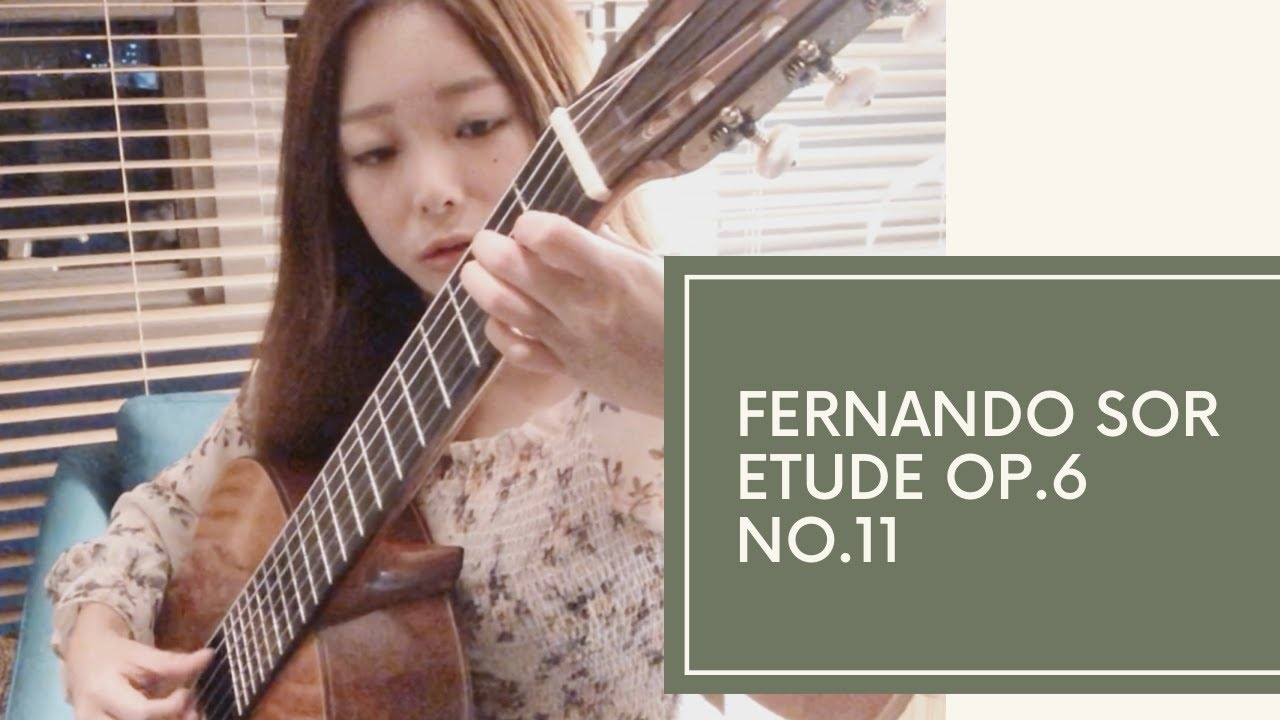
\includegraphics[width=0.48\linewidth]{pictures/youtube/2025/01/20250102_003401_youtube_001_q8UXw36AN9E.jpg}
}
\end{center}




2025年の新年はJ.S.BachのBWV998のPreludeでスタートしようと年末から決めていたのに、気がついたら、このF.Sorの曲の練習をしていた。


この曲は昔（学生の頃に）練習してみた事があったのだけど、見事に忘れてしまっている。出だしはいいんだけど、そのうちしばらくすると、、、こんなに指を伸ばさなければならなかったっけ？（６弦のGから１弦のBまでちょっと遠いよ。でも、聖母の御子で6弦DropのGから1弦のDまで伸ばしていたことを思えば、この程度のストレッチは普通にある事なんだろう、きっと）

\subsection*{2025年01月02日 09:02}
\addcontentsline{toc}{subsection}{2025年01月02日 09:02}

\url{https://www.facebook.com/share/p/1BG9BVet7z/}




綺麗です

自分でもこんな写真を撮りたいとなると、撮影データがとっても貴重（ありがたい）です（撮影地の情報がないのはちょっと残念）


12/29の5:39 （月の出は5:18）の撮影

（月齢27.5=新月の２日前）


140mmのレンズ（でアンタレスと水星も入って、月のサイズはこんな感じ）ISO1600、f4で2.5秒（で地球照も写る可能性）


f2.8なら1.25秒で、あるいはISO3200なら開放f4のレンズでも1.25秒でいけるかもしれない（ISO3200でも画質があまり落ちないと期待しての事です）


アンタレスと月だけなら、もう少し長い焦点距離のレンズで月も多少大きめにできるかもしれない（地球照のディテールも、となると高画素機が必要か）空の美しいグラデーションが画面に占める割合との兼ね合いもある


などなど、自分で撮影するときのシミュレーションをしてみています

（レンズなどの実機は持ち合わせていないので）

\subsection*{2025年01月05日 23:00}
\addcontentsline{toc}{subsection}{2025年01月05日 23:00}

これはとっても魅力的な曲なのですが、セーハの連続が厳しくて、音にならなくなってしまいます。この曲は絶対ハイレベルな演奏者向けだと思います。私は途中で何度もめげてしまっています。その内最後まで弾けるようになりたいのですが。（この曲は、私的には、この方↓の演奏がベストです）


\url{https://youtu.be/3D0WOvs0tcc}

\begin{center}
\href{https://youtu.be/3D0WOvs0tcc}{
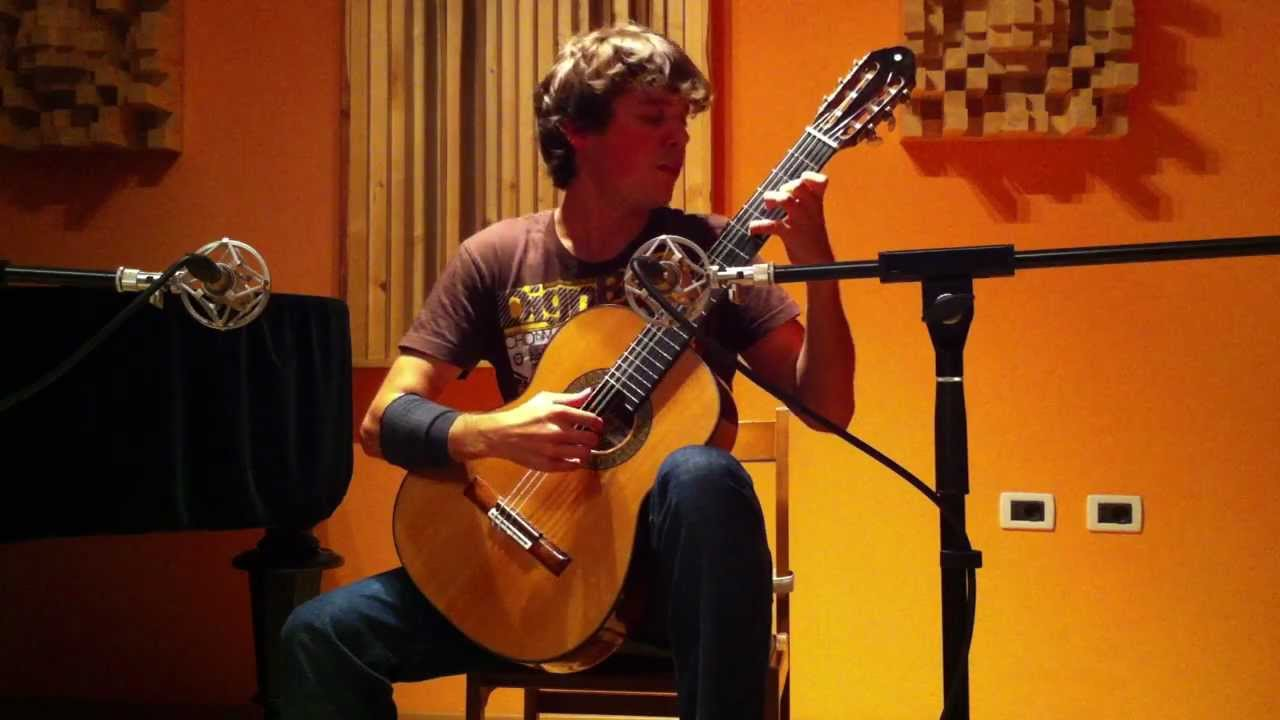
\includegraphics[width=0.48\linewidth]{pictures/youtube/2025/01/20250105_230039_youtube_001_3D0WOvs0tcc.jpg}
}
\end{center}



\subsection*{2025年01月12日 22:28}
\addcontentsline{toc}{subsection}{2025年01月12日 22:28}

\paragraph{リンク}
\url{https://youtu.be/ggxTit1M-C4}

\begin{center}
\href{https://youtu.be/ggxTit1M-C4}{
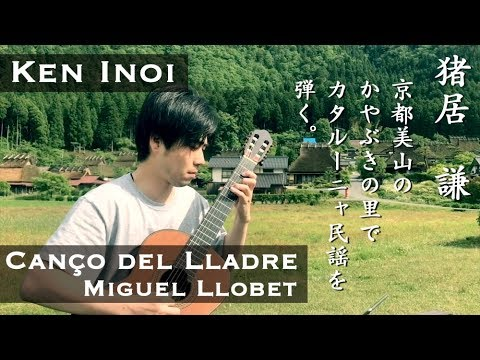
\includegraphics[width=0.48\linewidth]{pictures/youtube/2025/01/20250112_222815_youtube_001_ggxTit1M-C4.jpg}
}
\end{center}

\subsection*{2025年01月13日 19:09}
\addcontentsline{toc}{subsection}{2025年01月13日 19:09}

\url{https://www3.nhk.or.jp/news/html/20240921/k10014588341000.html}



\url{https://www.nhk.jp/p/dosuken/ts/G9W71XY6L3/list/}




貴景勝の言葉、思い出すたびに涙が溢れてくる。


「手をいっぱい伸ばしたんですけど、届きませんでした。」


その体格では幕内には上がれないだろうと言われた。

幕内に上がったら、三役は無理だろうと言われた。

大関になったら、突き押し相撲では横綱は無理だと言われた。


引退の時の言葉「相撲を始めた時に横綱になることだけ考えてきて、手をいっぱい伸ばしたんですけど、届きませんでした。」


貴景勝が、怪我を言い訳にする事なく、ストイックに、もがき、あがいていた。横綱になろうとしていた。真摯な取り組みの姿を毎場所見てきたから「手をいっぱい伸ばしたんですけど、、、」を聞くと目頭が熱くなる。本当に頑張っていたよね、頑張っている一生懸命な姿を見せてくれたね、としか言えなくなる。


（みんな大リーグで活躍する夢を叶えた人ばっかりじゃないんだよネ）

\paragraph{写真}
\begin{center}
\begin{minipage}{0.48\linewidth}
\centering
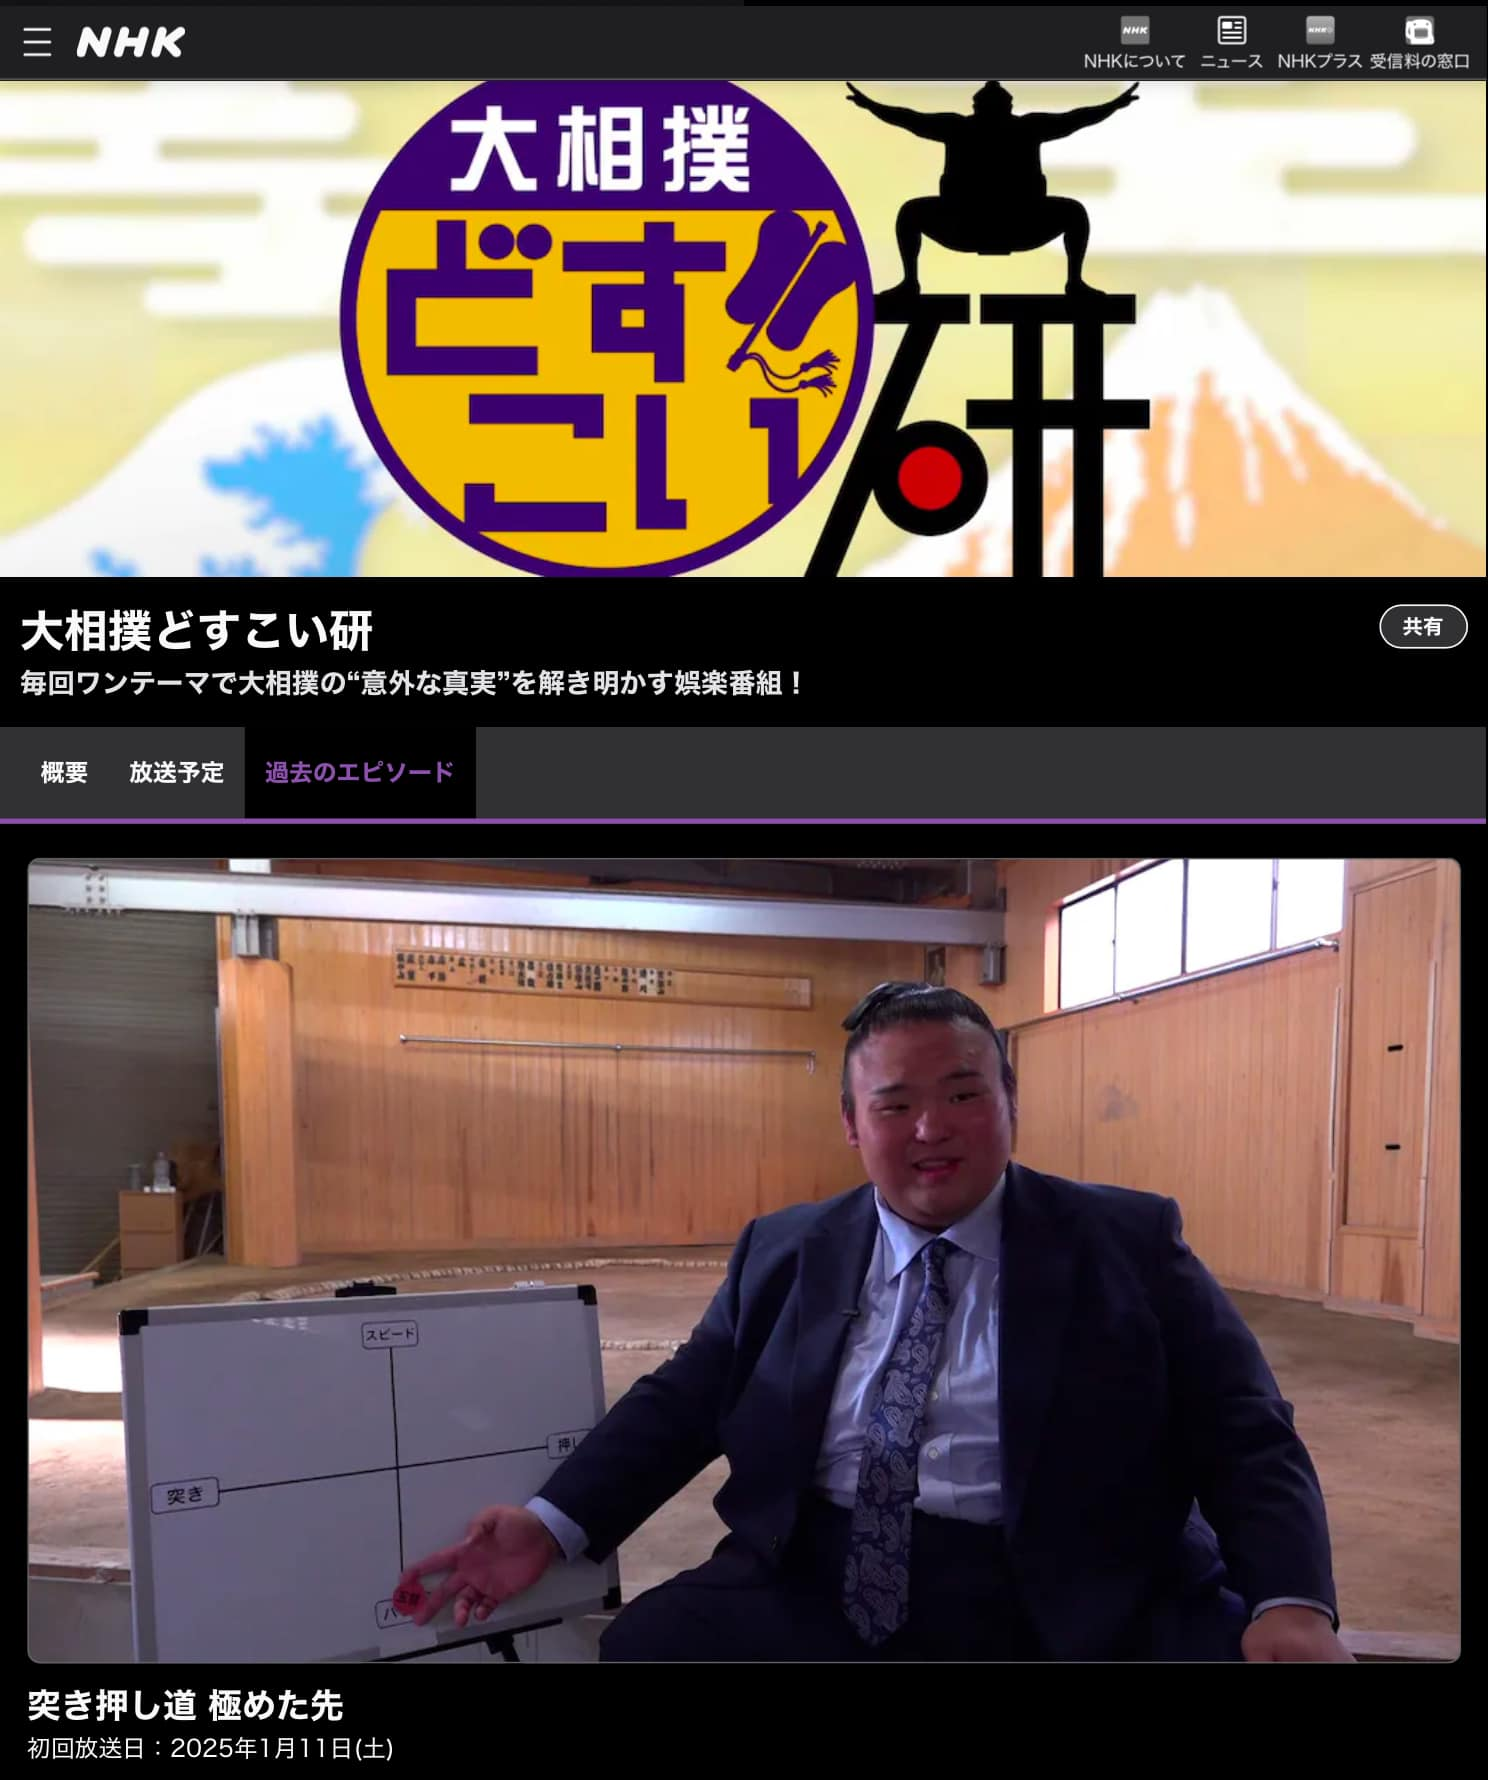
\includegraphics[width=\linewidth]{pictures/2025/01/20250113_190914_001.jpg}
\end{minipage}
\end{center}

\subsection*{2025年01月13日 23:01}
\addcontentsline{toc}{subsection}{2025年01月13日 23:01}

\url{https://youtu.be/DvCM3jHLwxU}

\begin{center}
\href{https://youtu.be/DvCM3jHLwxU}{
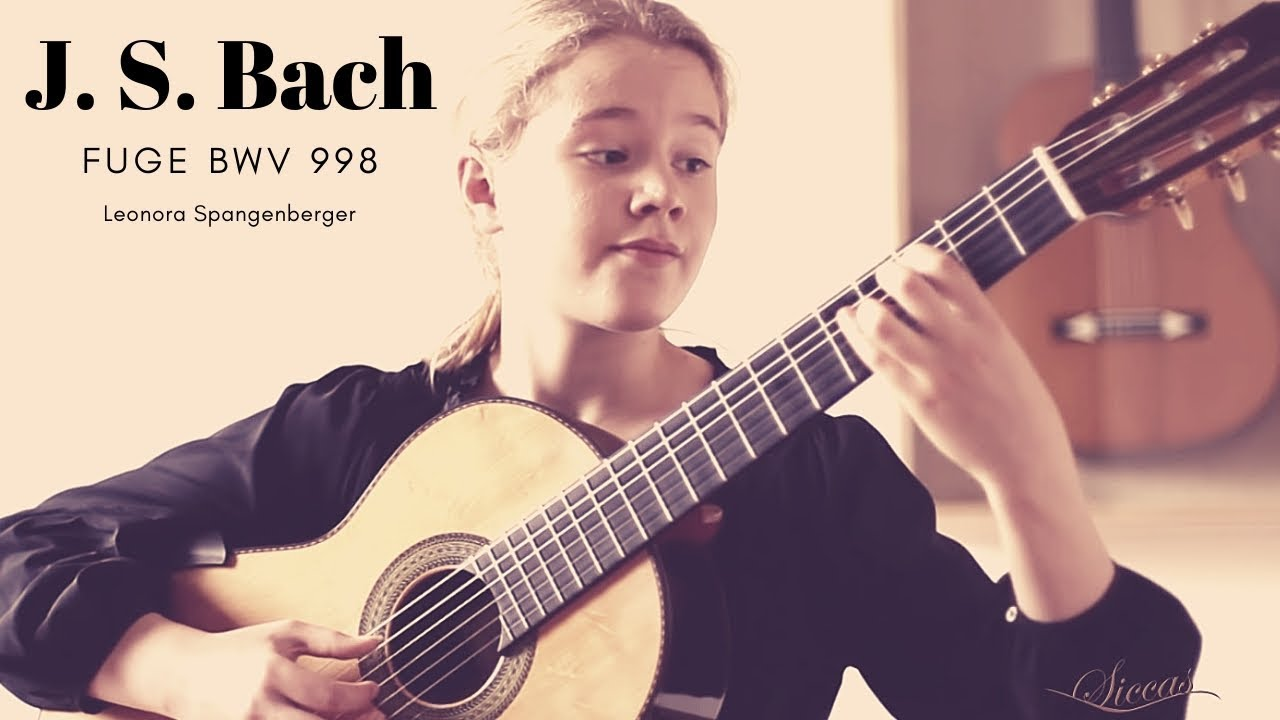
\includegraphics[width=0.48\linewidth]{pictures/youtube/2025/01/20250113_230135_youtube_001_DvCM3jHLwxU.jpg}
}
\end{center}




BWV998のfugueの攻略に着手。


決してPreludeの演奏を完成させたから先に進むという訳ではない。実のところ、どれだけ弾いてみてもダメダメだという気持ちしかない。（進歩していない＝プラトー＝高原状態＝スランプ なのか？一人合宿してPrelude漬けでもしてみる？）発表会の機会でもあれば、うまくいってもいかなくても何らかの区切りがつくのかもしれないけど、そうでない以上キリが（つか）ないのだ。なので新年を一つの契機（キリ）にする事として、2025年一年をかけたfugueの攻略に踏み出してみる事にした。（途中で諦める事になるかも、、）


この曲はちょっと長いよ。とり敢えず前半（三分の一あたり？分散和音みたいな所に入る前まで）の攻略を目指すことにしよう。Preludeの時と同じ様に、セゴビア編の楽譜を下敷きに、運指を決める事から始めていこうと思います。（が、この方の演奏を見ると、そもそも出だしの主題提示部からいきなりセゴビア編とは運指が異なっている\textasciicircum{}\textasciicircum{};）


先は長そうだけど、ゆっくり行こう。ゆっくり。

\subsection*{2025年01月14日 12:43}
\addcontentsline{toc}{subsection}{2025年01月14日 12:43}

これはどなたの編曲でしょう？ご自身の手によるものかもしれません。

高い音域から始まっているのが特徴的で、好きな編曲です。


\url{https://youtu.be/5Tj9T9BFaJc}

\begin{center}
\href{https://youtu.be/5Tj9T9BFaJc}{
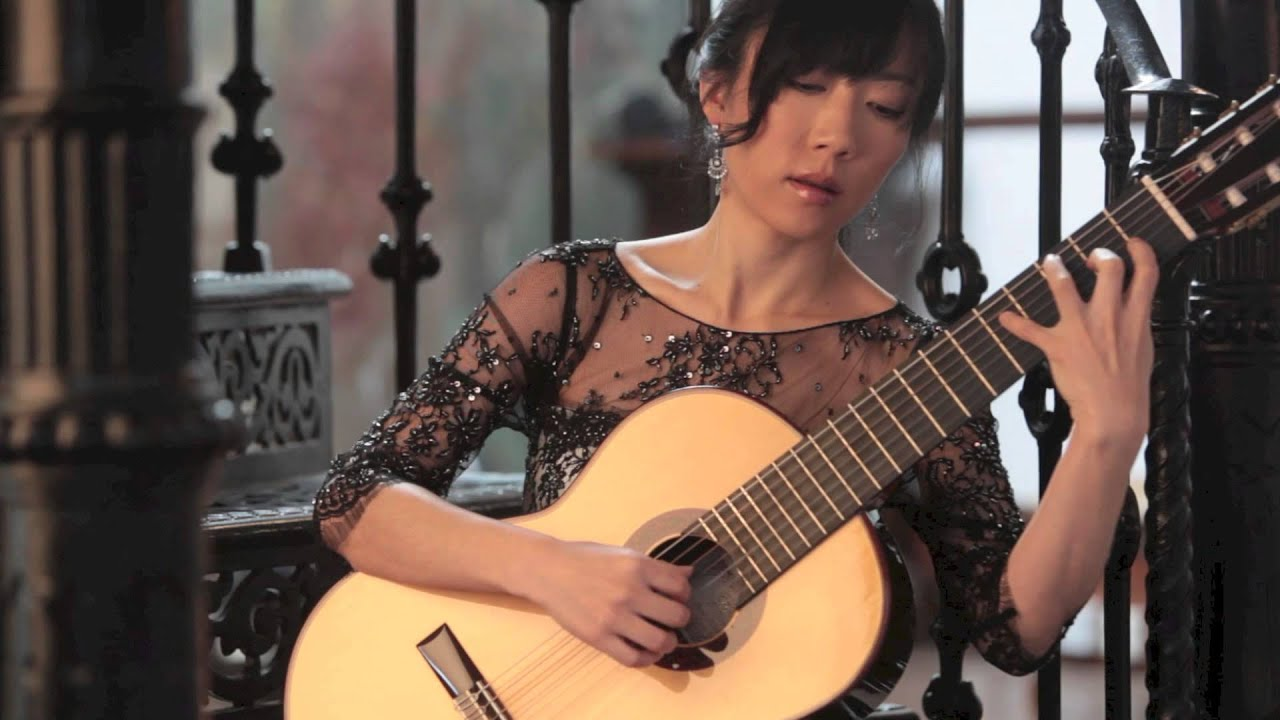
\includegraphics[width=0.48\linewidth]{pictures/youtube/2025/01/20250114_124355_youtube_001_5Tj9T9BFaJc.jpg}
}
\end{center}




指揮者のハンス・フォン・ビュロウは、J.S.Bachの平均律クラヴィーア曲集を旧約聖書、ベートーヴェンのピアノ・ソナタを新約聖書だと言ったとか、、、

\subsection*{2025年01月14日 16:12}
\addcontentsline{toc}{subsection}{2025年01月14日 16:12}

\paragraph{リンク}
\url{https://youtu.be/eW5tZGuQnOU}

\begin{center}
\href{https://youtu.be/eW5tZGuQnOU}{
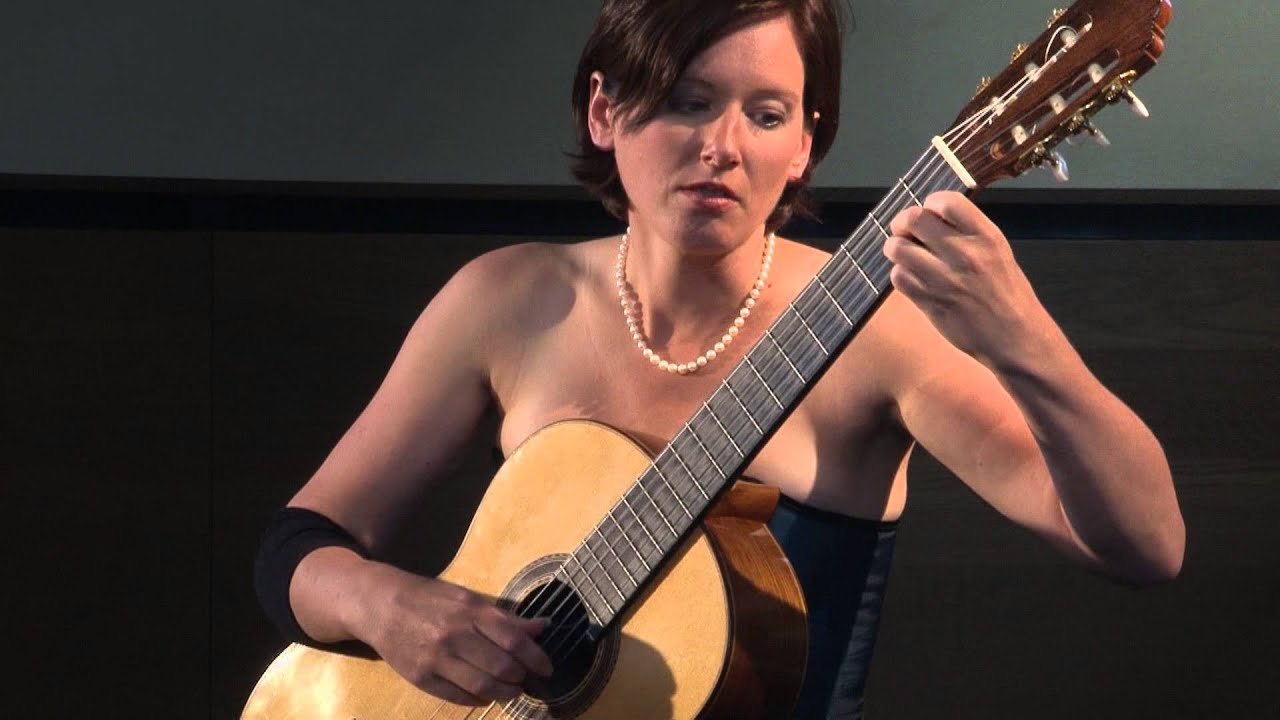
\includegraphics[width=0.48\linewidth]{pictures/youtube/2025/01/20250114_161205_youtube_001_eW5tZGuQnOU.jpg}
}
\end{center}

\subsection*{2025年01月14日 16:37}
\addcontentsline{toc}{subsection}{2025年01月14日 16:37}

\paragraph{リンク}
\url{https://youtu.be/5FP0tXMqrIo}

\begin{center}
\href{https://youtu.be/5FP0tXMqrIo}{
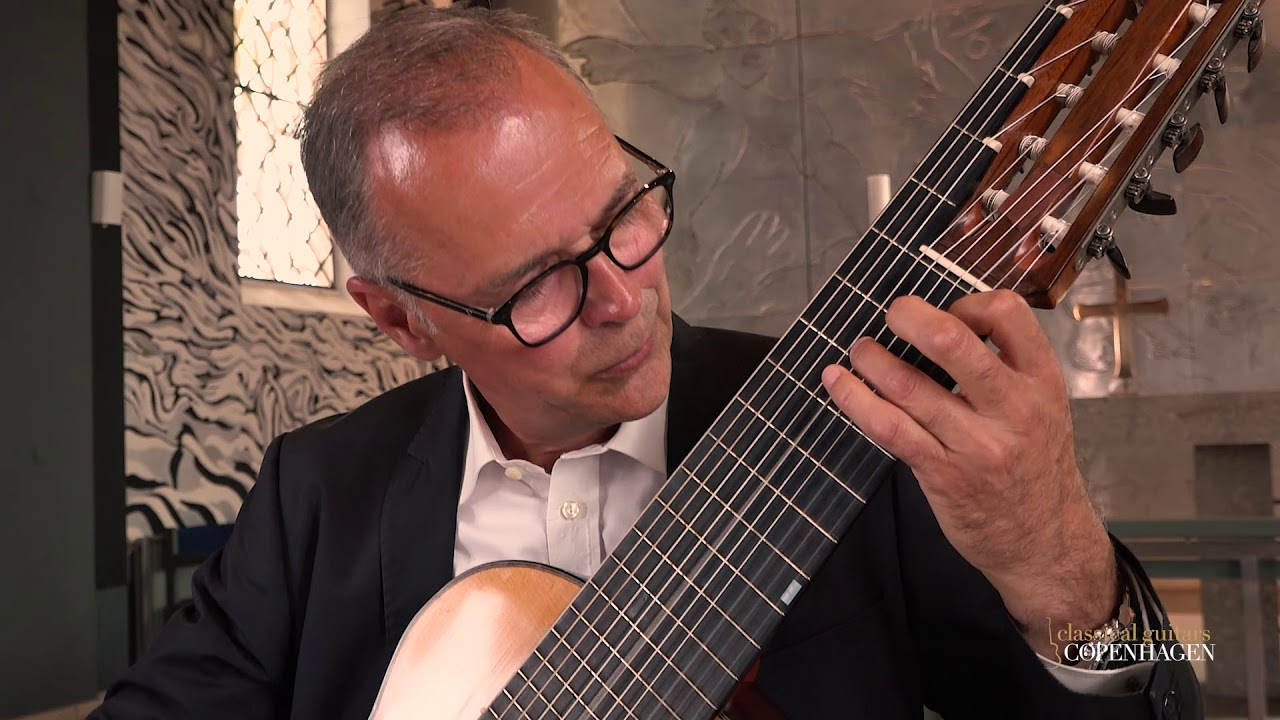
\includegraphics[width=0.48\linewidth]{pictures/youtube/2025/01/20250114_163711_youtube_001_5FP0tXMqrIo.jpg}
}
\end{center}

\subsection*{2025年01月16日 13:18}
\addcontentsline{toc}{subsection}{2025年01月16日 13:18}

\paragraph{リンク}
\url{https://youtu.be/tEcEjGHUnNI}

\begin{center}
\href{https://youtu.be/tEcEjGHUnNI}{
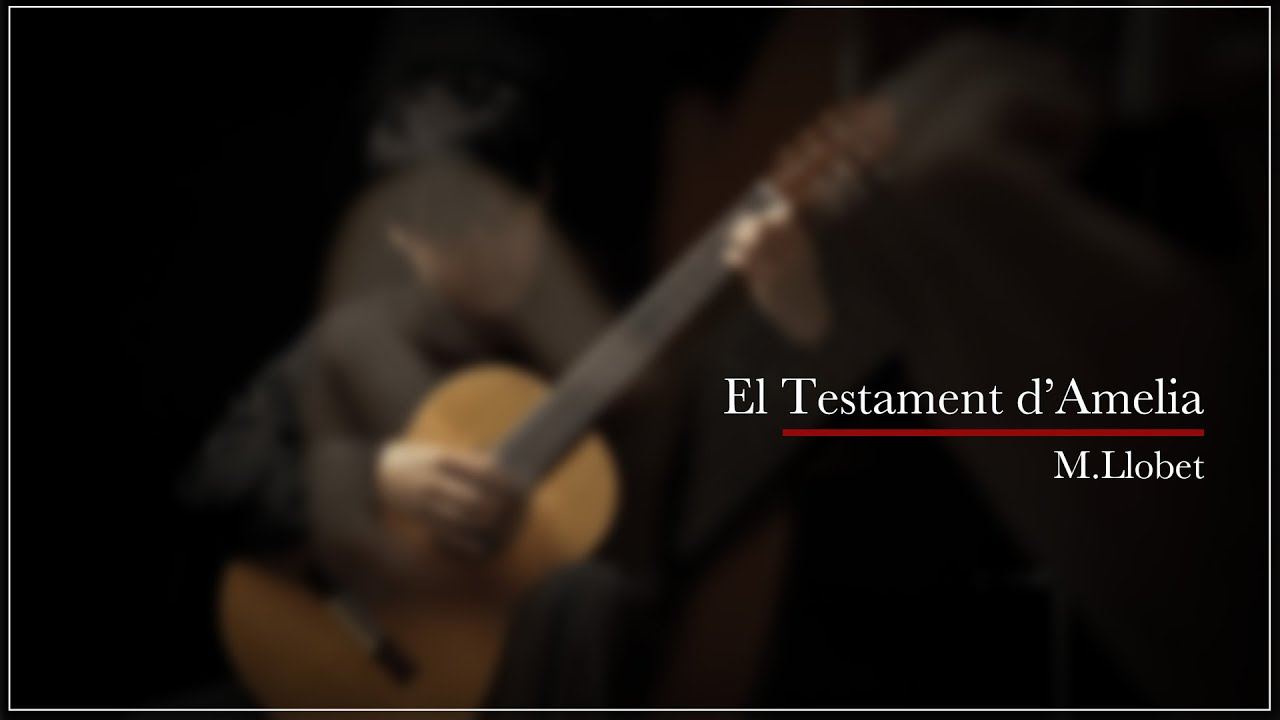
\includegraphics[width=0.48\linewidth]{pictures/youtube/2025/01/20250116_131829_youtube_001_tEcEjGHUnNI.jpg}
}
\end{center}

\subsection*{2025年01月16日 13:22}
\addcontentsline{toc}{subsection}{2025年01月16日 13:22}

\paragraph{リンク}
\url{https://youtu.be/UcOwTJlHnV8}

\begin{center}
\href{https://youtu.be/UcOwTJlHnV8}{
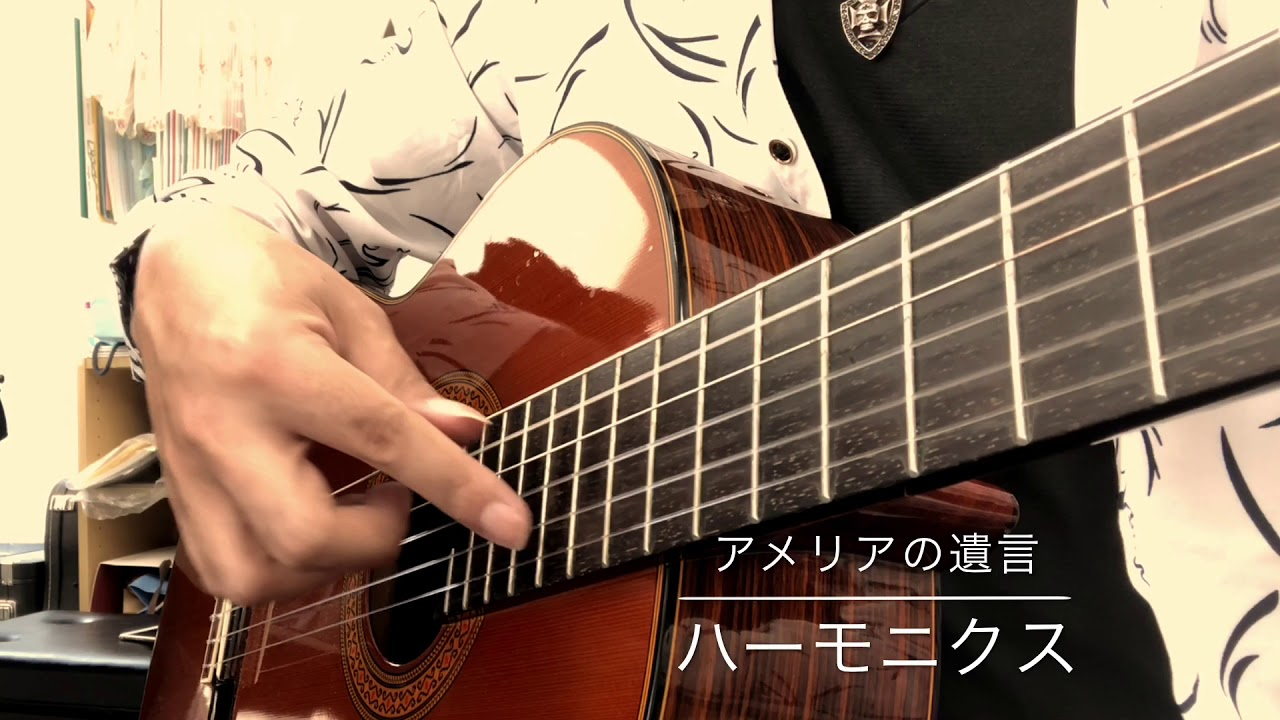
\includegraphics[width=0.48\linewidth]{pictures/youtube/2025/01/20250116_132250_youtube_001_UcOwTJlHnV8.jpg}
}
\end{center}

\subsection*{2025年01月17日 08:41}
\addcontentsline{toc}{subsection}{2025年01月17日 08:41}

\url{https://youtu.be/_XxCU7mghj8}

\begin{center}
\href{https://youtu.be/_XxCU7mghj8}{
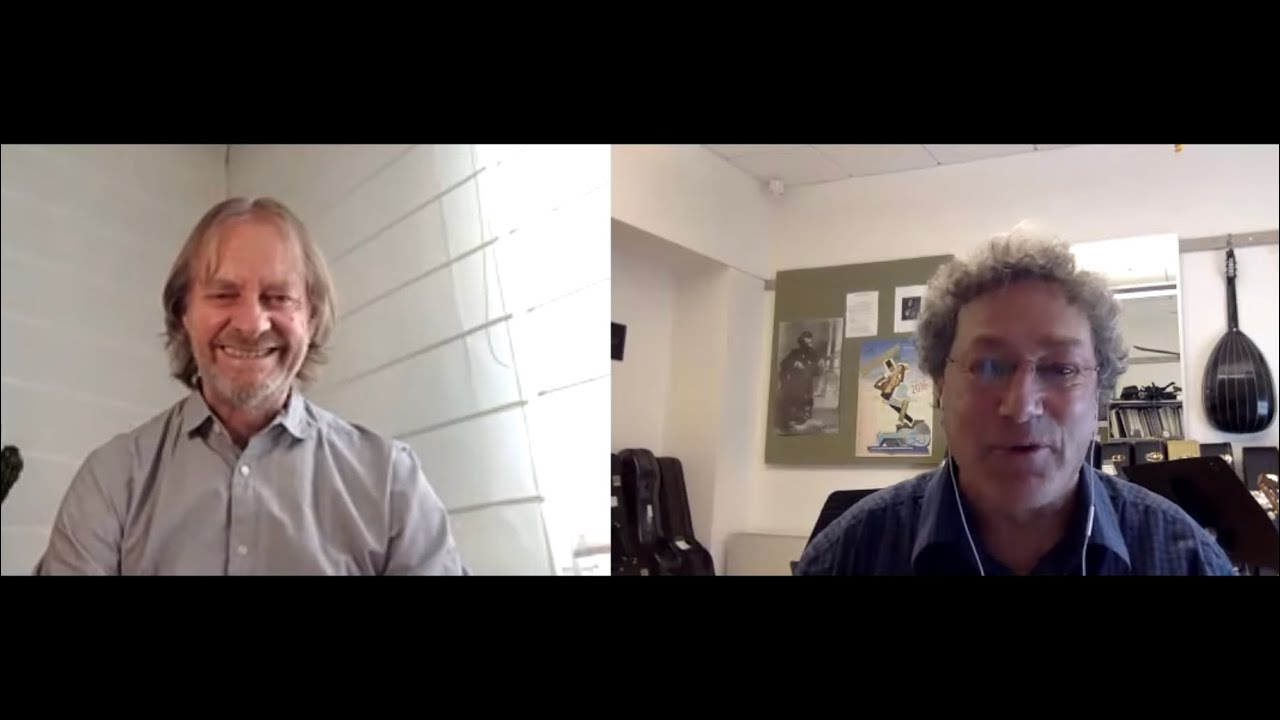
\includegraphics[width=0.48\linewidth]{pictures/youtube/2025/01/20250117_084118_youtube_001__XxCU7mghj8.jpg}
}
\end{center}




二人のDavidによるBWV998に関する対話

（Youtubeに日本語翻訳字幕機能があってよかったよ）


(１) ギターに適した（最もよく響く）調があるという事？


(２) Bachは「３」に（宗教的な）意味を重ねて（意識して）いただろうか？

⚪︎３楽章（Prelude, Fugue, Allegro）構成はJ.S.Bachでは唯一

⚪︎Fugueは３つの部分からなる構造

⚪︎フラットが３つ


(３) 「ため息」の音形（修辞法の話）は確かにFugueで繰り返されている様な気がする

\subsection*{2025年01月17日 08:56}
\addcontentsline{toc}{subsection}{2025年01月17日 08:56}

\paragraph{リンク}
\url{https://youtu.be/HNrq-j3wzM4}

\begin{center}
\href{https://youtu.be/HNrq-j3wzM4}{
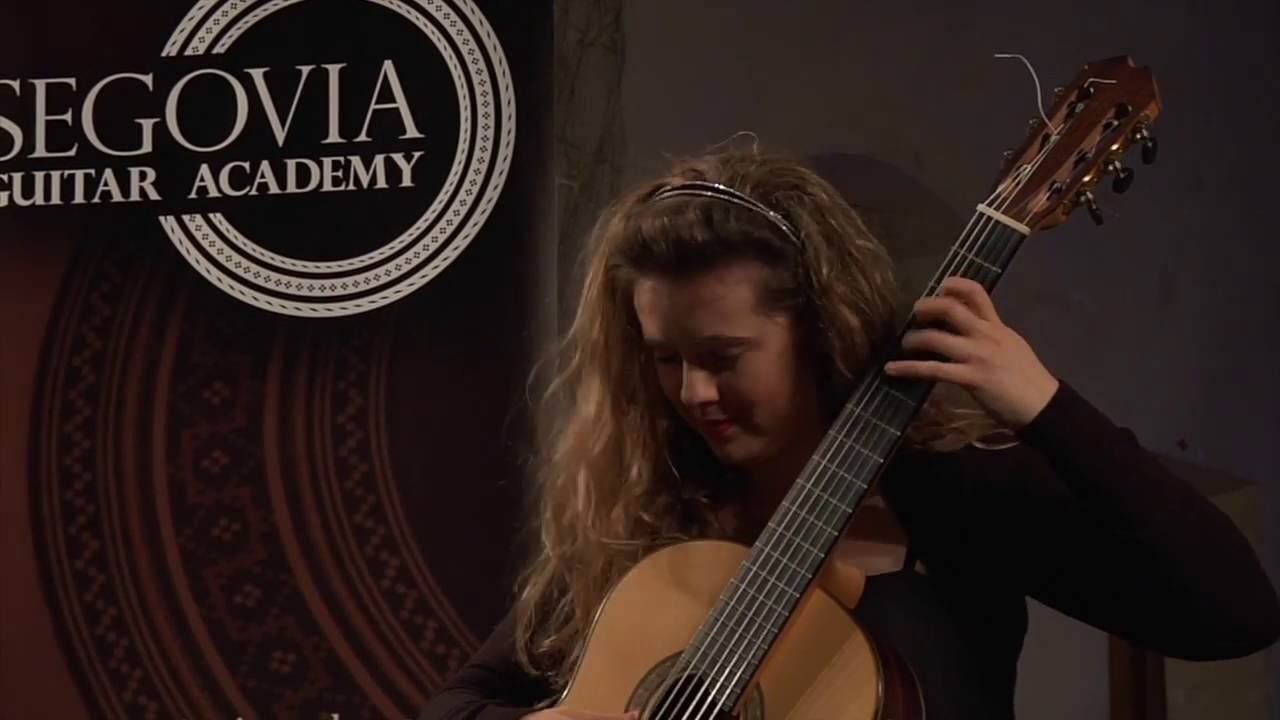
\includegraphics[width=0.48\linewidth]{pictures/youtube/2025/01/20250117_085638_youtube_001_HNrq-j3wzM4.jpg}
}
\end{center}

\subsection*{2025年01月17日 08:57}
\addcontentsline{toc}{subsection}{2025年01月17日 08:57}

\paragraph{リンク}
\url{https://youtu.be/OosoIH6osS0}

\begin{center}
\href{https://youtu.be/OosoIH6osS0}{
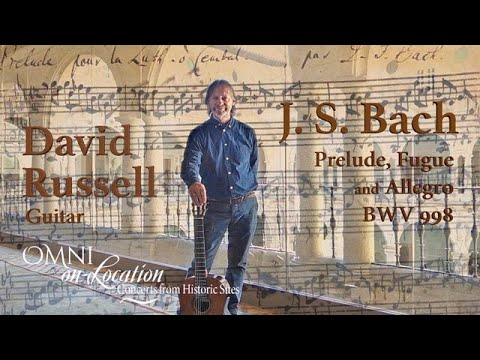
\includegraphics[width=0.48\linewidth]{pictures/youtube/2025/01/20250117_085731_youtube_001_OosoIH6osS0.jpg}
}
\end{center}

\subsection*{2025年01月17日 08:58}
\addcontentsline{toc}{subsection}{2025年01月17日 08:58}

\paragraph{リンク}
\url{https://youtu.be/yiGrgOV-wiQ}

\begin{center}
\href{https://youtu.be/yiGrgOV-wiQ}{
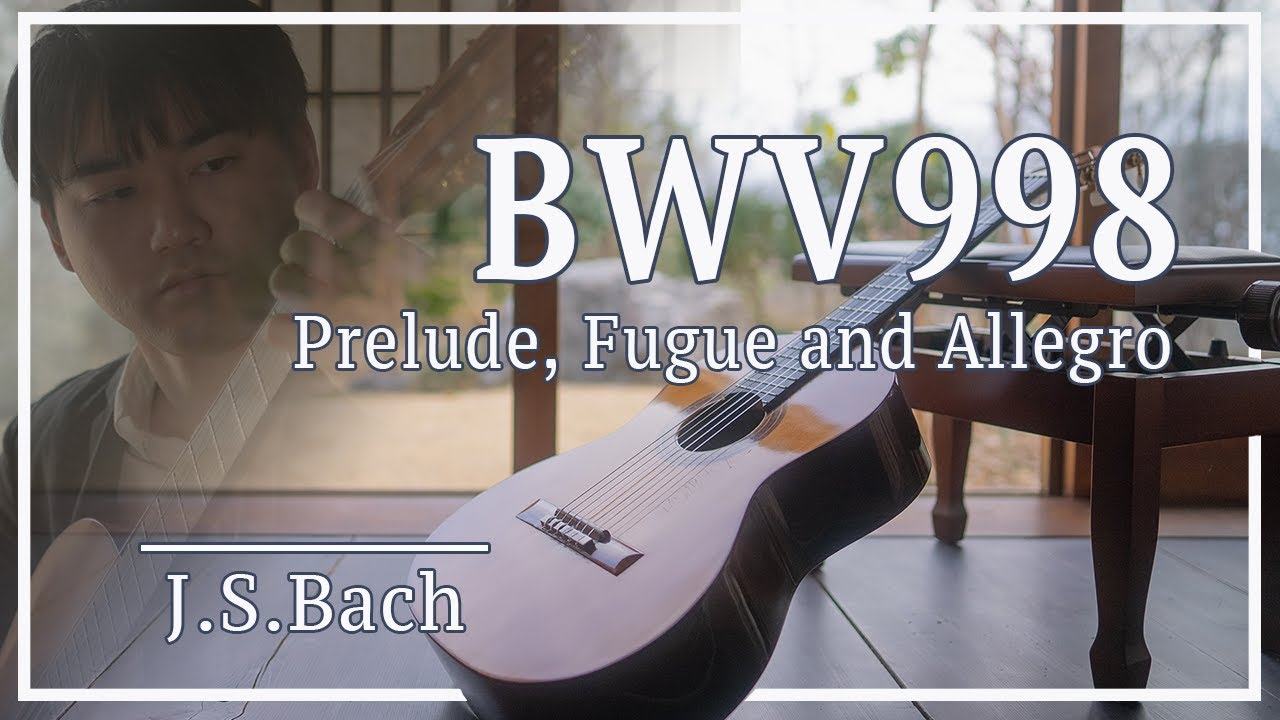
\includegraphics[width=0.48\linewidth]{pictures/youtube/2025/01/20250117_085851_youtube_001_yiGrgOV-wiQ.jpg}
}
\end{center}

\subsection*{2025年01月17日 12:58}
\addcontentsline{toc}{subsection}{2025年01月17日 12:58}

\paragraph{リンク}
\url{https://youtu.be/dFd26PI6jiE}

\begin{center}
\href{https://youtu.be/dFd26PI6jiE}{
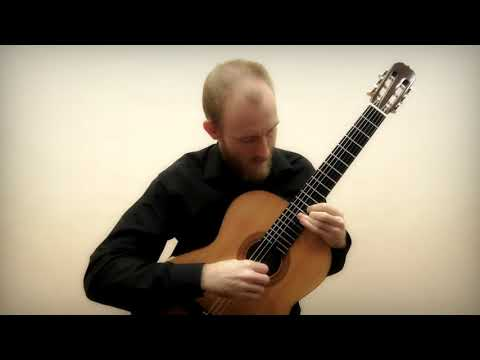
\includegraphics[width=0.48\linewidth]{pictures/youtube/2025/01/20250117_125838_youtube_001_dFd26PI6jiE.jpg}
}
\end{center}

\subsection*{2025年01月19日 16:06}
\addcontentsline{toc}{subsection}{2025年01月19日 16:06}

今日の散歩。

5.1km、1時間32分。

実に天気が良い。


犀川雪見橋をわたって、

御参詣坂（最大心拍数はここ）を登り、

市立病院前、平和町を通って、

不老坂を降り、

上菊橋を渡って、戻りました。


御参詣坂を登ったのは初めてですが、かなり急な坂で息が切れます。

夜街灯がついているのは、この坂なのかな？

（途中私の様な年齢層の方の散歩と多く出会っている様な気がします）

\paragraph{写真}
\begin{center}
\begin{minipage}{0.48\linewidth}
\centering
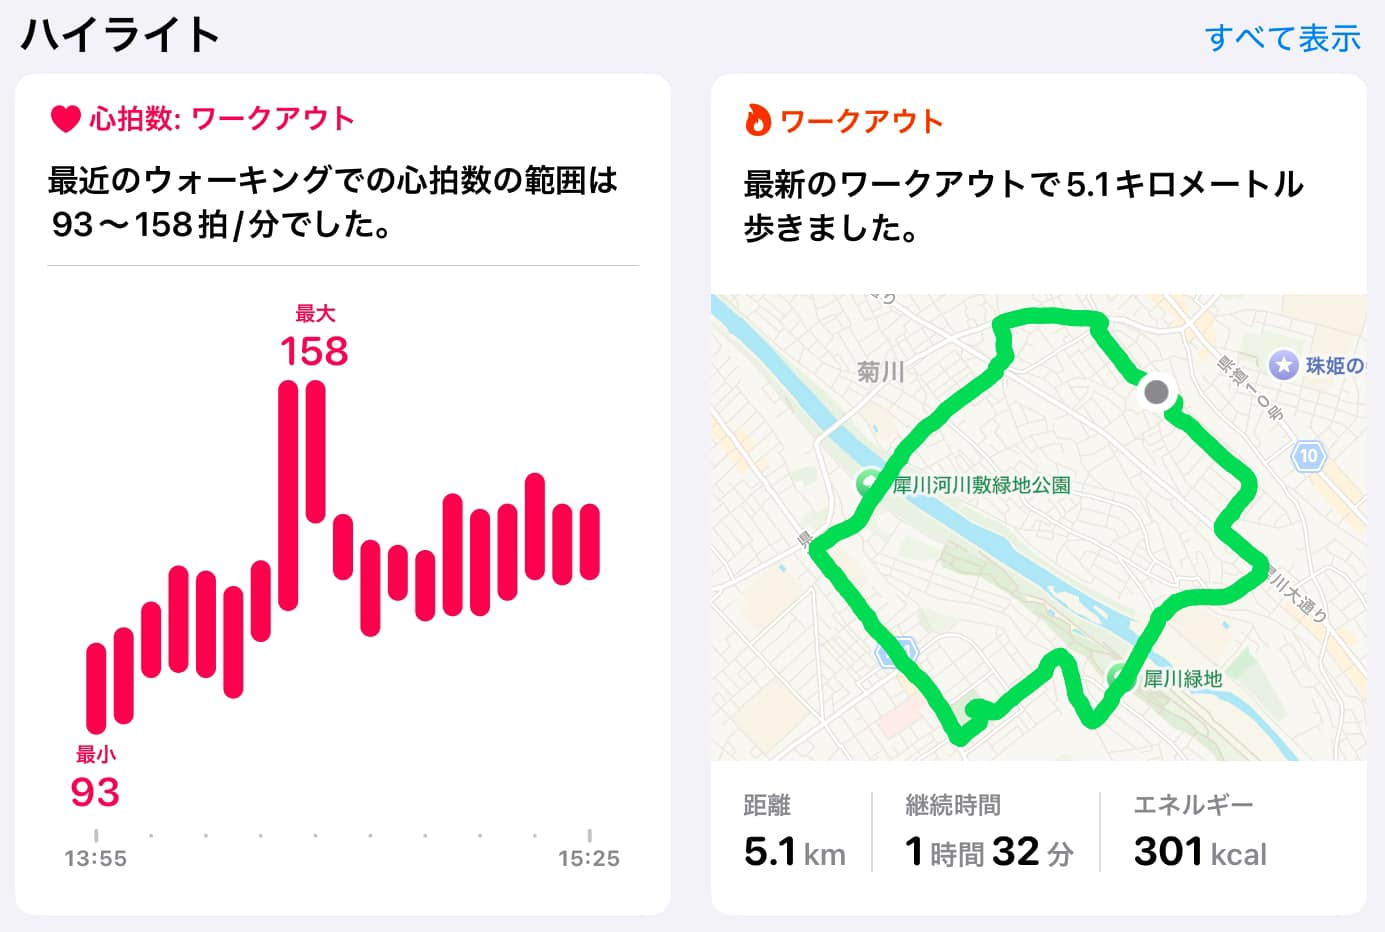
\includegraphics[width=\linewidth]{pictures/2025/01/20250119_160611_001.jpg}
\end{minipage}
\hfill
\begin{minipage}{0.48\linewidth}
\centering
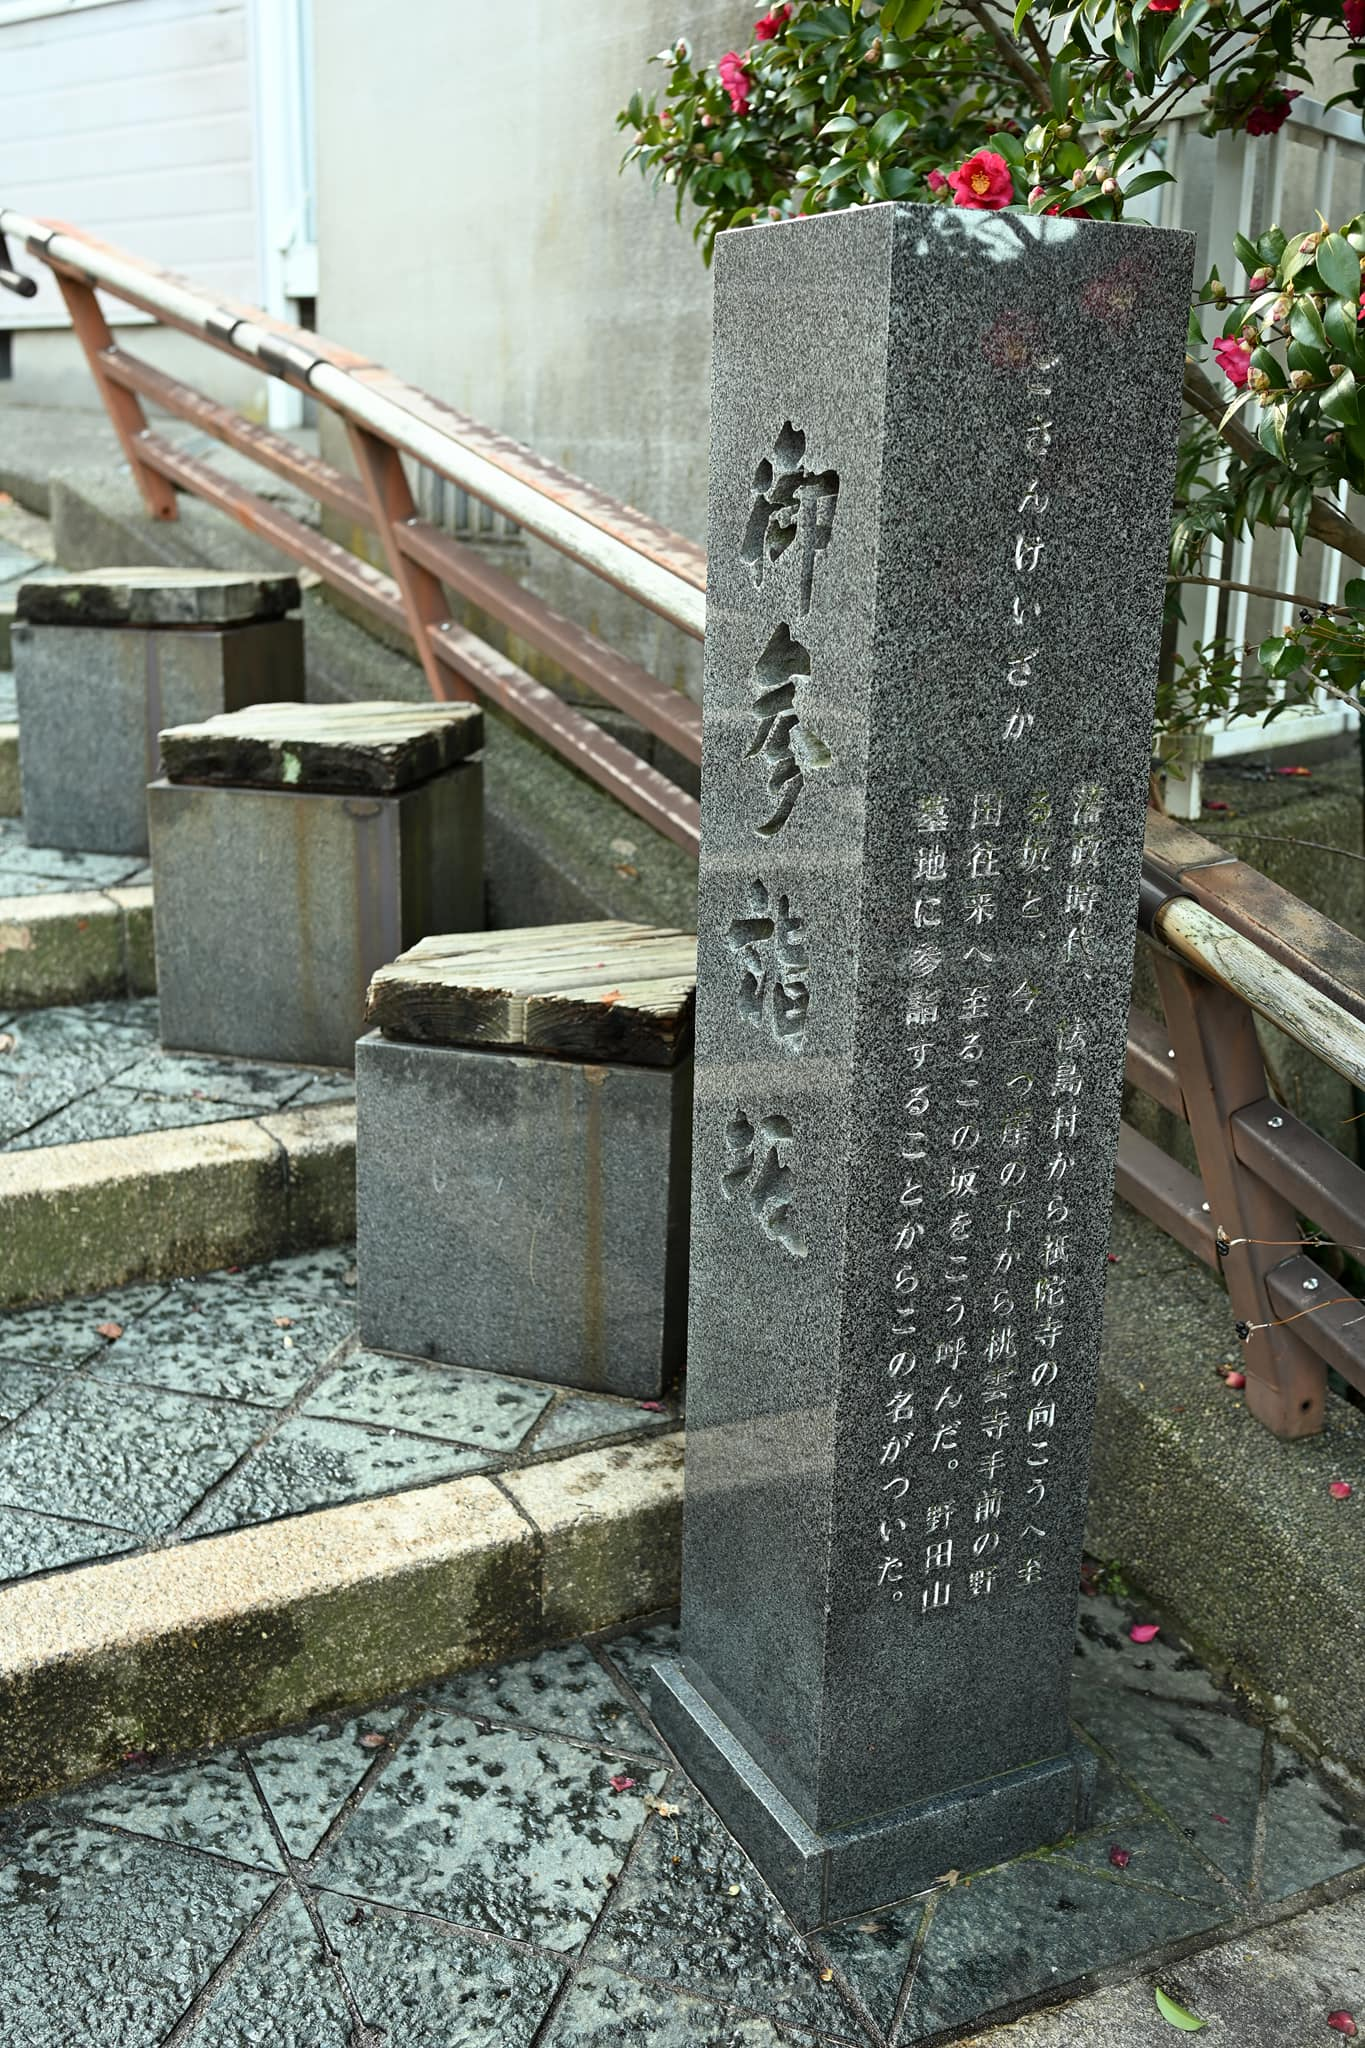
\includegraphics[width=\linewidth]{pictures/2025/01/20250119_160611_002.jpg}
\end{minipage}
\end{center}

\subsection*{2025年01月20日 15:53}
\addcontentsline{toc}{subsection}{2025年01月20日 15:53}

「\#聖母の御子 」「\#アメリアの遺言 」「\#盗賊の歌 」の３つについて、添付の本（どちらも \#現代ギター 社刊）で楽譜を比較してみた。以下、「ミゲル．\#リョベート 作品集」に載っている楽譜を「L」で、「てんこもり」に載っている楽譜を「T」で区別する事にする。


(１) 「アメリアの遺言」について（てんこもりのvol1）

「L」と「T」に違いはない様です。


(２) 「盗賊の歌」について（てんこもりのvol3）

違いは1箇所。

「T」の22小節目の3拍目の頭のA（八分音符）が、「L」ではAis。

「L」では13小節目（自然ハーモニクスのA）と違えるため、22小節目でわざわざAisにしているのか？（そもそも15小節目の前と後では、同じ主題ですが少しづつ趣向を変えて聞かせていますし。）それとも「T」は、3拍目の表から裏へのクロマティックな動き A→Aisを聞かせようという趣向なのか？


(３) 「聖母の御子」について（てんこもりのvol1）

違いがあり過ぎて、ここに列挙し切れない。（ここまで違うと、これは既に別の編曲なんでしょうね）

気になったのは、4小節目の後半、12小節目の後半、そして最終小節のリズムだ。例えば4小節目なら、「L」では8分音符→4分音符だが、「T」では4分音符→8分音符になっている。12小節目でも、「L」では8分音符→4分音符だが、「T」では付点4分音符1個になってしまっている。最終小節では「L」が16分休符→16分音符→8分音符の動きなのに対して、「T」では8分音符2つになってしまっている。（一応rit するだろうから、シンコペっぽい動きは薄れていって終わるとは思いますが、それを音符で書いてしまうというのもどうなのかな。）

4小節目前半最後の8分音符DGBの和音で、「L」ではGなのが「T」ではGis。（これはどういう事？「L」の誤植？）

10小節目のバス（6弦のDと4弦のD）の動きも異なっている。10小節目の終りの8分音符が11小節の頭（1弦のD）に向けたアウフタクトと見るなら、どっちの楽譜のDの動きが効果的なんだろうか。

最終小節の1つ前の小節で、「T」では和音を分散させている様ですが、これは演奏者のアドリブに委ねられる範囲かもしれません。


リョベートは、 \#カタロニア民謡 をギター譜に移して編曲した人として知られていますが、タレガとセゴビアの間の時代に活躍（タレガの弟子でセゴビアの恩師？）して、ギター音楽の発展に貢献のあった方だと「T」の解説にはありました。今日までの長い年月の間に色々と楽譜が書き換えられて伝えられている、或いは様々な編曲が存在している、これらはあり得る事なんだと思います。


（その後気付いたこと）

「T」の聖母の御子ですが、リョベート編だとはどこにも書かれていませんでした。単にカタロニア民謡とだけ書かれていました。従ってリョベート編とは別の編曲だという認識で良い様です。「T」には特に編曲者名が明記されていませんでしたが、一方で、盗賊の歌とアメリアの遺言については、「T」の解説でリョベート編であるとの記述が明記されていました。（編曲者名が明示された楽譜で弾きたいと言う気がします）

また「T」の解説によると、カタロニア民謡の聖母の御子を「最初に」編曲したのはリョベートですが、この曲はセゴビアの演奏（セゴビア編）によって広く知られる様になったとの事でした。


(細かなうんちくはさておき、実際に聖母の御子を演奏しようとすると、途切れ途切れのトツトツ演奏になってしまう(\textasciicircum{}\textasciicircum{};; こっちの方が問題だな）

\paragraph{写真}
\begin{center}
\begin{minipage}{0.48\linewidth}
\centering
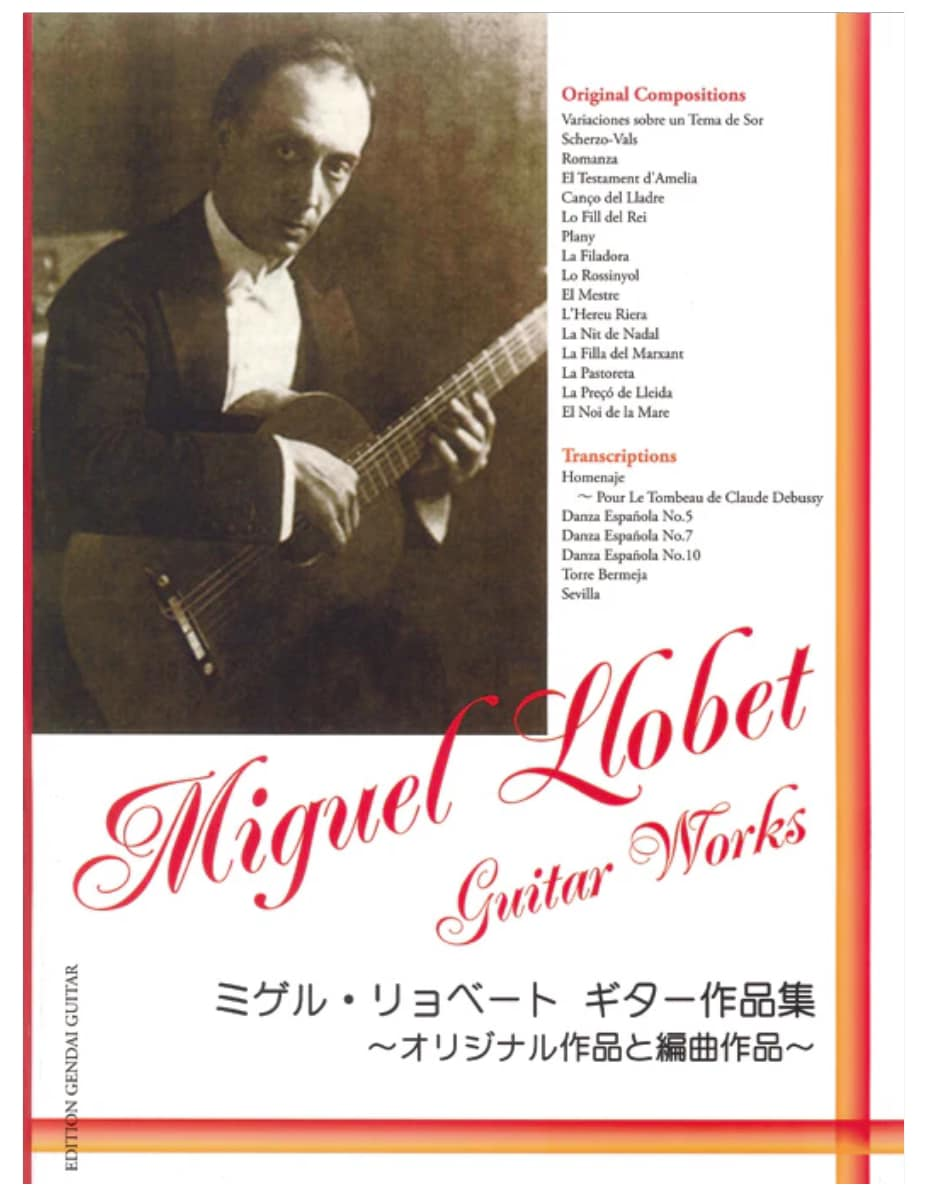
\includegraphics[width=\linewidth]{pictures/2025/01/20250120_155308_001.jpg}
\end{minipage}
\hfill
\begin{minipage}{0.48\linewidth}
\centering
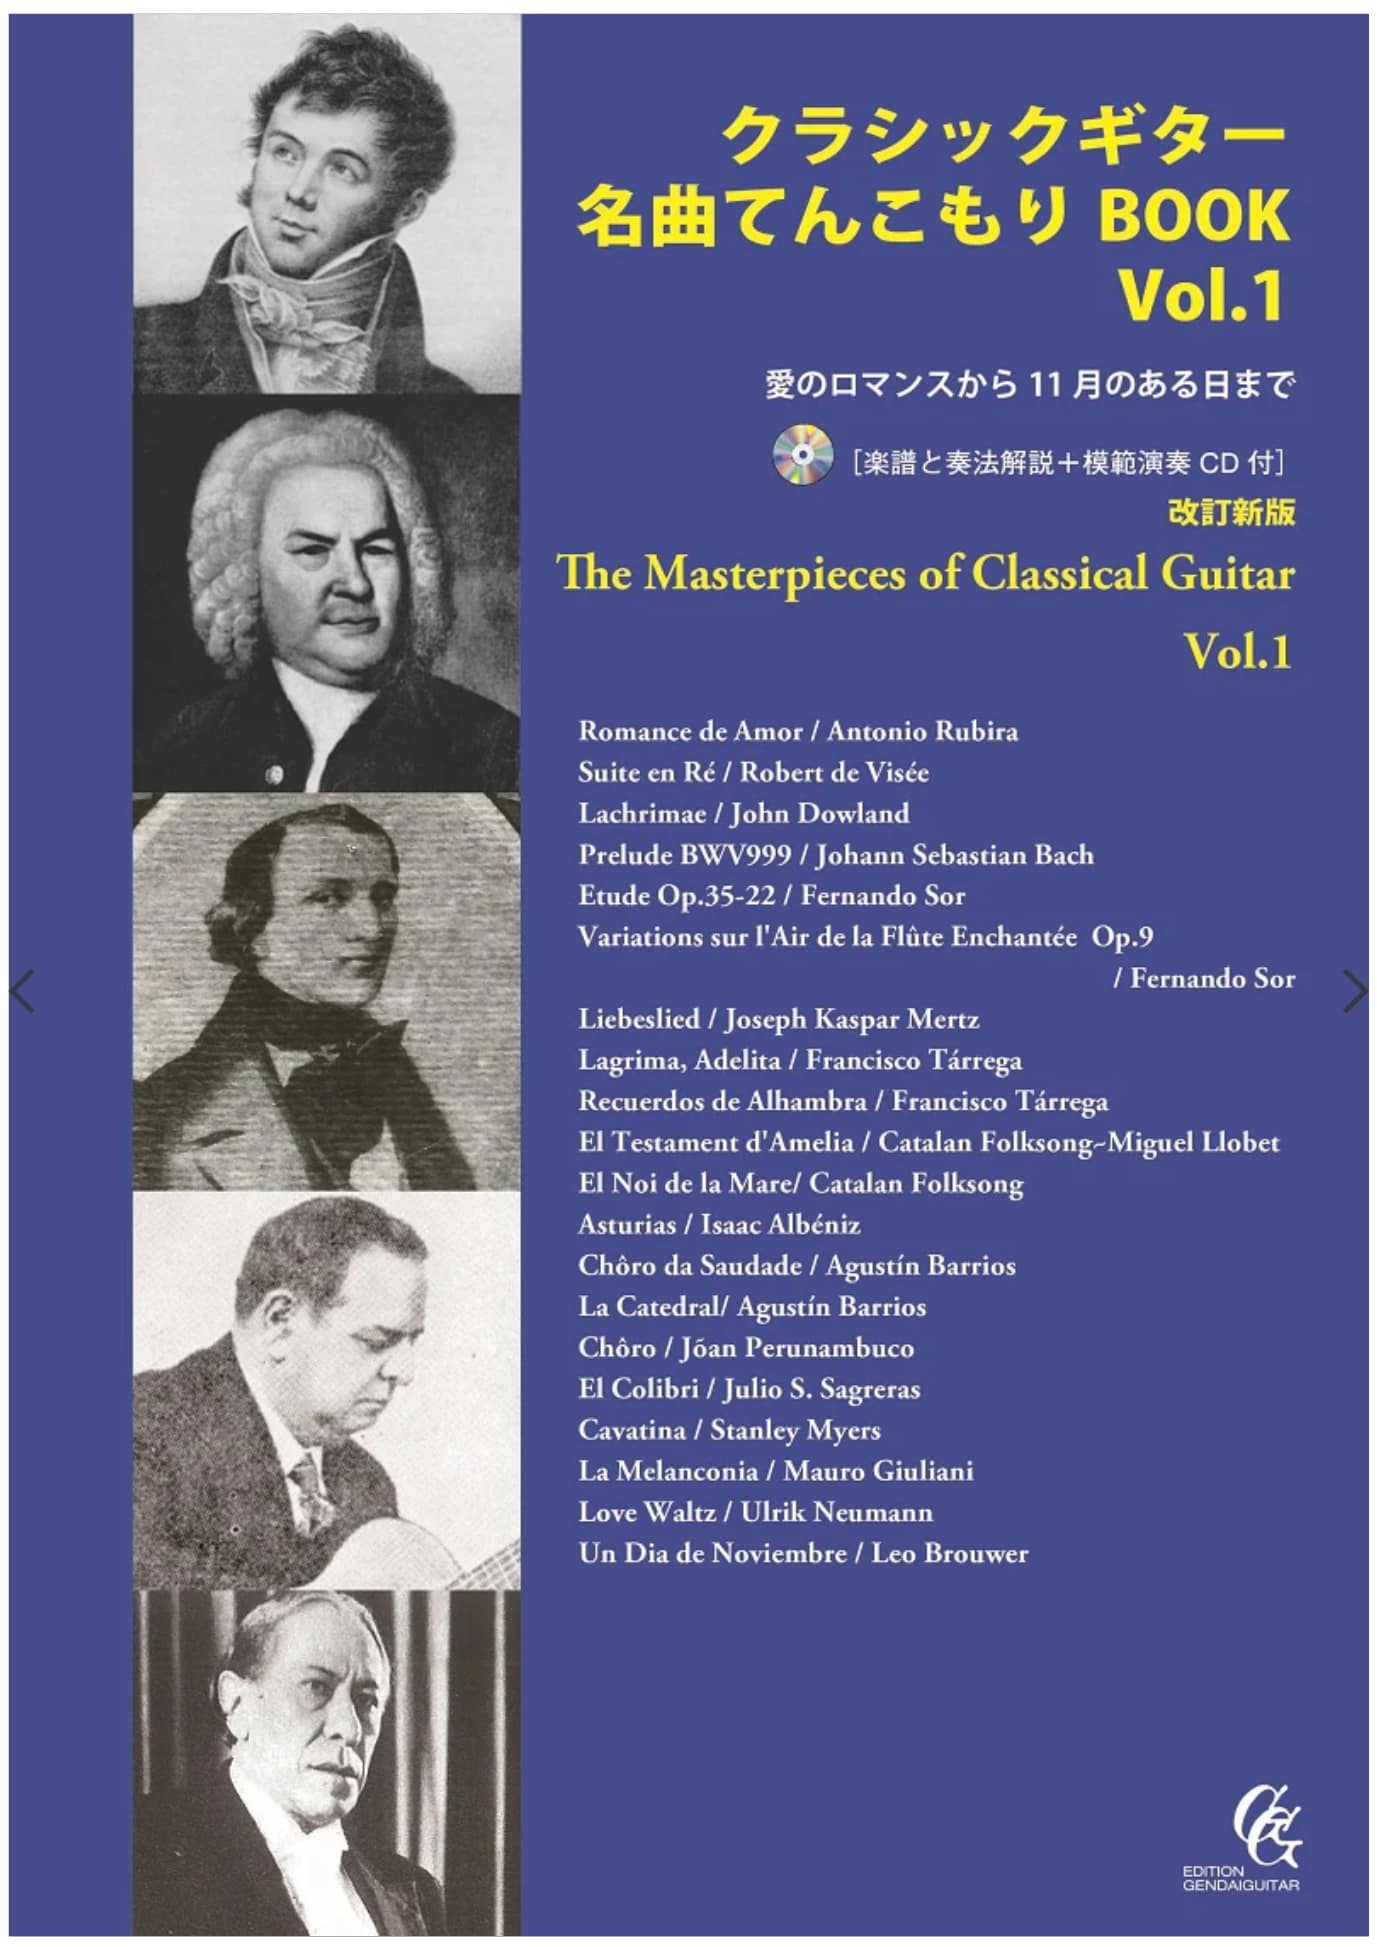
\includegraphics[width=\linewidth]{pictures/2025/01/20250120_155308_002.jpg}
\end{minipage}
\end{center}

\subsection*{2025年01月22日 19:44}
\addcontentsline{toc}{subsection}{2025年01月22日 19:44}

\paragraph{リンク}
\url{https://youtu.be/qN1W-ogDeR0}

\begin{center}
\href{https://youtu.be/qN1W-ogDeR0}{
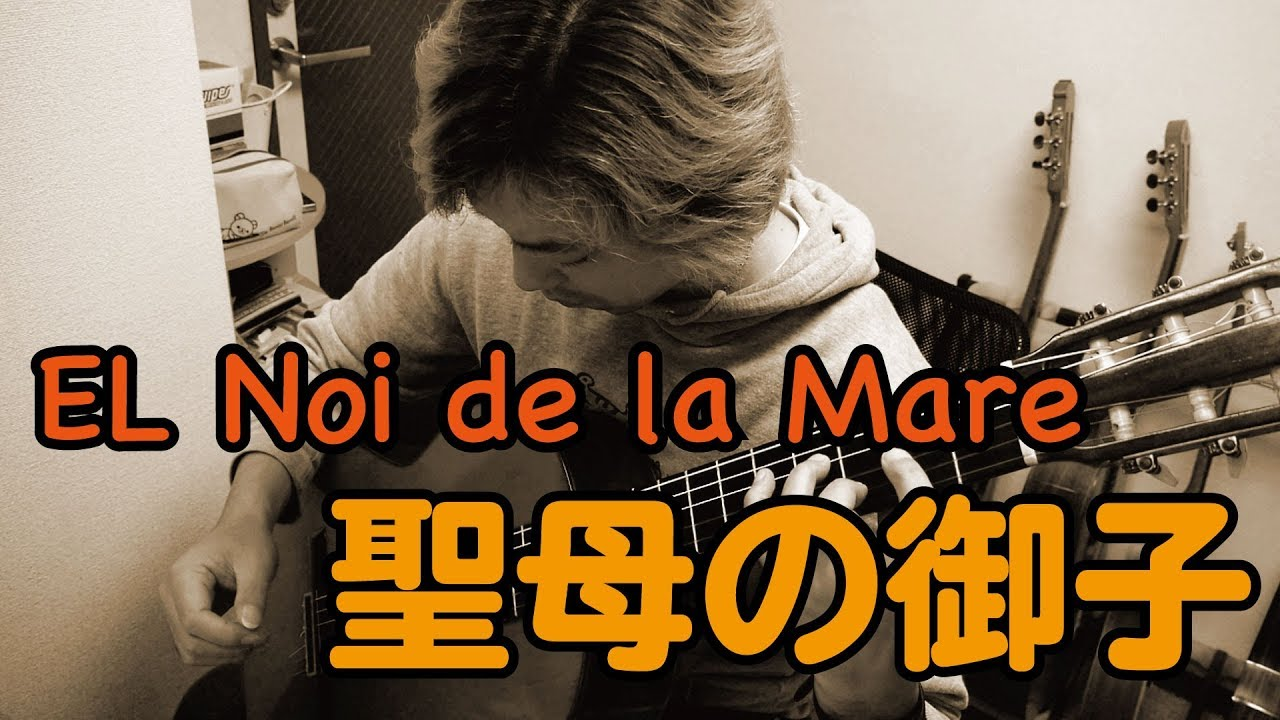
\includegraphics[width=0.48\linewidth]{pictures/youtube/2025/01/20250122_194432_youtube_001_qN1W-ogDeR0.jpg}
}
\end{center}

\subsection*{2025年01月24日 09:04}
\addcontentsline{toc}{subsection}{2025年01月24日 09:04}

時々、「XXさんからのあなたのアクティビティが閲覧できる様になりました。」というのが知らされるんだけど、この日本語のメッセージの意味を理解できない。


主語は何なのか？「XXさんからのあなたのアクティビティ」とは何なのか？私のアクティビティなのか、XXさんの何らかのアクティビティなのか？XXさんの私に対するアクティビティって何かあるのか？そもそもアクティビティとは投稿した記事のことを指すのか？いいねボタンを押したことか？コメントした内容の事か？それらの全てか？（英文のメッセージを安物翻訳ソフトにかけて無理やり日本語にしたみたいに見える。元々の英文メッセージを見てみたいものだ。）


とりあえず「XXさんがあなたのアクティビティ（投稿した記事）を閲覧しました。」という様な意味かと勝手に思っているが、、、

\subsection*{2025年01月24日 15:53}
\addcontentsline{toc}{subsection}{2025年01月24日 15:53}

\paragraph{リンク}
\url{https://youtu.be/yhsgUNr8ZWg}

\begin{center}
\href{https://youtu.be/yhsgUNr8ZWg}{
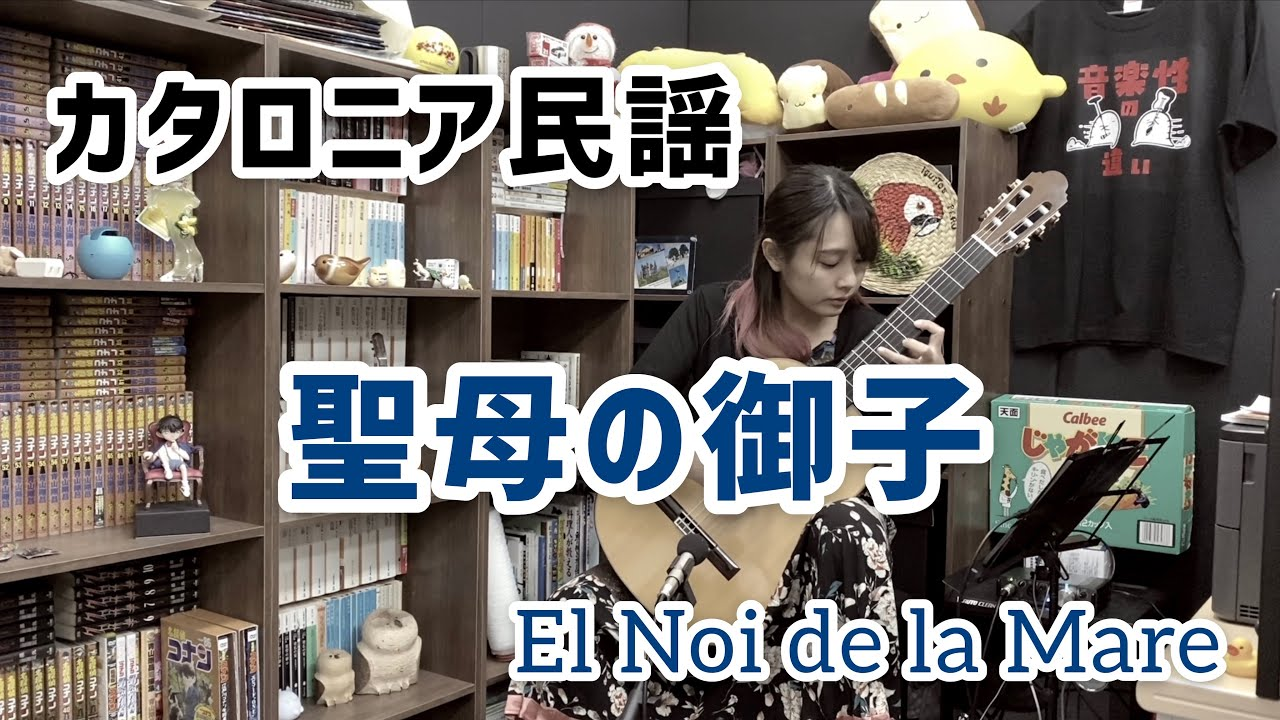
\includegraphics[width=0.48\linewidth]{pictures/youtube/2025/01/20250124_155318_youtube_001_yhsgUNr8ZWg.jpg}
}
\end{center}

\subsection*{2025年01月24日 16:32}
\addcontentsline{toc}{subsection}{2025年01月24日 16:32}

\paragraph{リンク}
\url{https://youtu.be/pyLhgyIpunQ}

\begin{center}
\href{https://youtu.be/pyLhgyIpunQ}{
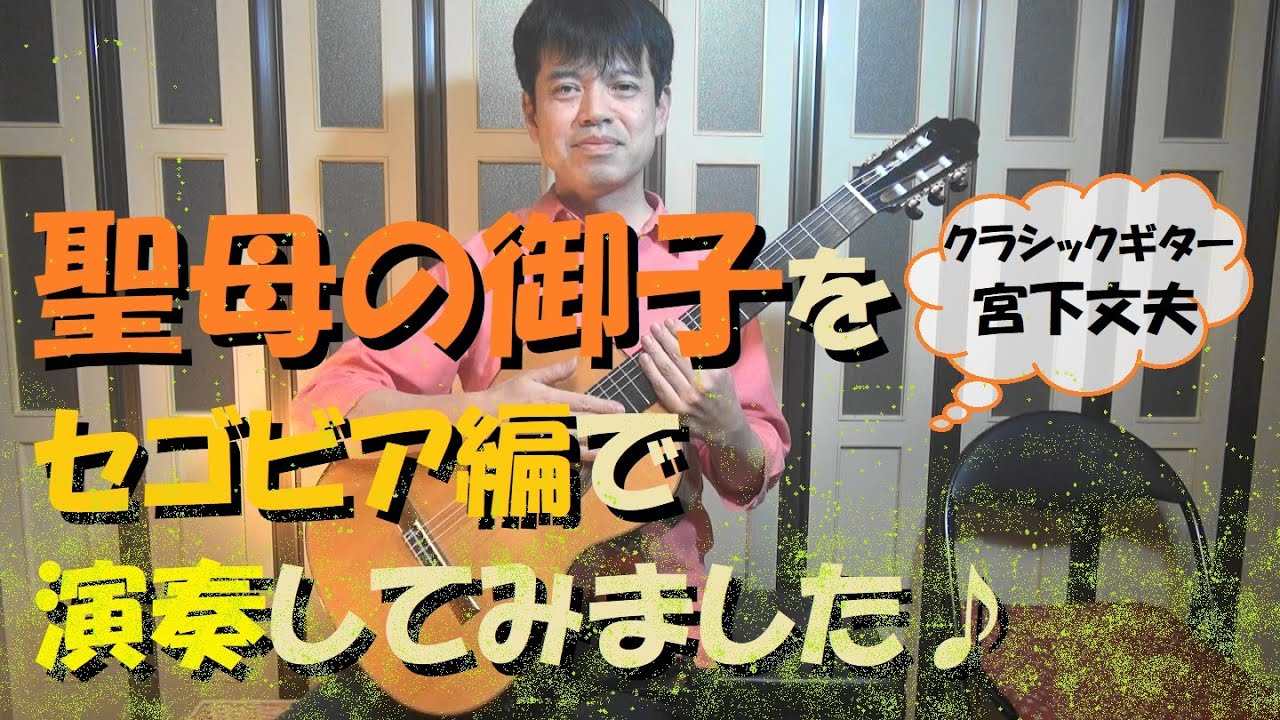
\includegraphics[width=0.48\linewidth]{pictures/youtube/2025/01/20250124_163237_youtube_001_pyLhgyIpunQ.jpg}
}
\end{center}

\subsection*{2025年01月25日 10:12}
\addcontentsline{toc}{subsection}{2025年01月25日 10:12}

\paragraph{リンク}
\url{https://youtu.be/HWfYd5SANHY}

\begin{center}
\href{https://youtu.be/HWfYd5SANHY}{
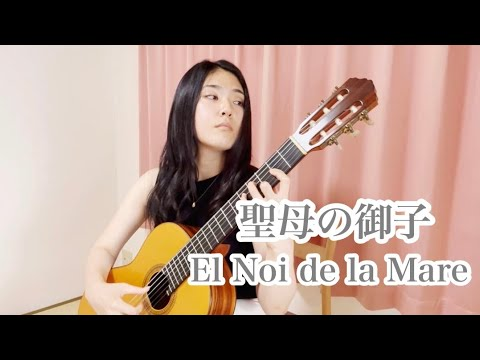
\includegraphics[width=0.48\linewidth]{pictures/youtube/2025/01/20250125_101259_youtube_001_HWfYd5SANHY.jpg}
}
\end{center}

\subsection*{2025年01月25日 12:07}
\addcontentsline{toc}{subsection}{2025年01月25日 12:07}

\paragraph{リンク}
\url{https://youtu.be/FX1lZPoF3Eo}

\begin{center}
\href{https://youtu.be/FX1lZPoF3Eo}{
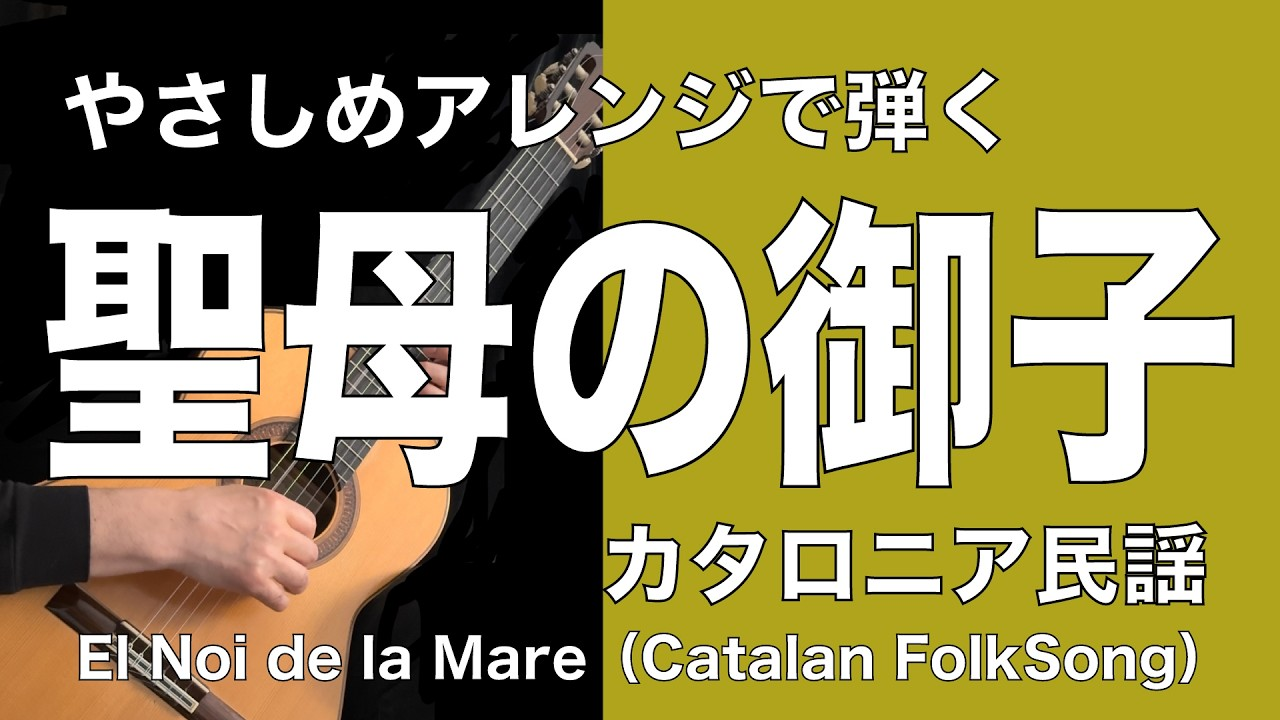
\includegraphics[width=0.48\linewidth]{pictures/youtube/2025/01/20250125_120711_youtube_001_FX1lZPoF3Eo.jpg}
}
\end{center}

\subsection*{2025年01月31日 08:55}
\addcontentsline{toc}{subsection}{2025年01月31日 08:55}

\url{https://altema.is.tohoku.ac.jp/QA4U3/}



量子コンピュータをプログラムできる（無料）と言うので、この \#QA4U3 というプロジェクトに参加してみることにした。受講している方々は多様です。大学生や院生はいるだろうと思っていましたが、社会人、サラリーマンもいらっしゃる様ですし、私の様な年齢の者もいるかと思えば、何と！高校生も参加している。素敵なプロジェクトだ。


第一回（1月31日）

\url{https://youtu.be/ZTIoDjfDSSw}

\begin{center}
\href{https://youtu.be/ZTIoDjfDSSw}{
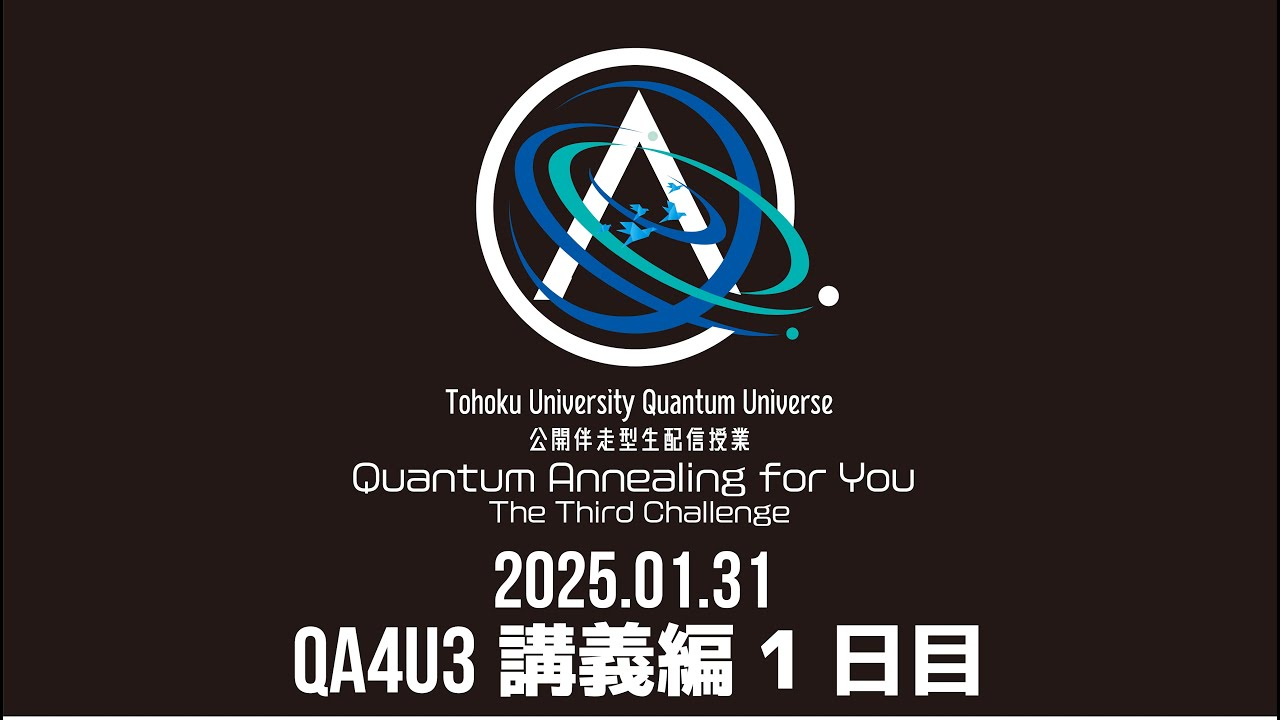
\includegraphics[width=0.48\linewidth]{pictures/youtube/2025/01/20250131_085534_youtube_001_ZTIoDjfDSSw.jpg}
}
\end{center}



量子コンピュータのシミュレータ（openjij）を使って、量子アニーリング、及びシミュレーテッド.アニーリングでのプログラム作りを体験した。磁性体を磁化する（スピンの向きを揃える）模擬実験。操作するスピンの数Nの多い場合に、温度Tの逆数（逆温度β）を大きくしていく（温度Tを下げていく）と、ある所で急激にスピンの向きが揃いはじめる（相転移を生じる）という現象を、Pythonのプログラムによる模擬実験の結果（グラフ表示）から示せた。（スピンの数Nが少ないと相転移の現象は現れない）


添付はNが10、100、1000、5000の各場合についてシミュレーテッド.アニーリングによる実験をしてみたもの。

スピンの向きは例えば上向きを＋1、下向きを－1とするけれども、スピンが上向きに揃っても下向きに揃っても、どちらも揃っている状態とみなしたいので、平均値を自乗して0から1の範囲の数にしている。縦軸が0に近いのはスピンの向きがバラバラな状態（無秩序相）、1に近いのはスピンの向きが（上でも下でもいいけどどちらかの向きに）揃っている状態（秩序相）。横軸は逆温度なので、左が高温で右へ行くほど低温。

そもそもNが小さいとガタガタグラフだが、num\_sweepsが小さい場合も十分に焼きなましが完了せず時間切れになってガタガタしたグラフになる。サンプル試行回数のnum\_readsが小さくてもガタガタする様になる。Nが1000では、はっきりとした相転移が見えてくる。


スピンの向きを2値（Binary）であると割り切る事で、それを実社会における様々な事象や人間の行動に対応させて、いろいろな社会問題の解決に、量子コンピュータを使ったプログラムで対峙していこうというプロジェクトの様だ。第二回（2月7日）以降では、シミュレータではなく、実際の量子コンピュータをプログラムで操作する予定らしい。


\#量子 \#量子コンピュータ \#アニーリング \#量子アニーリング \#スピン \#QA4U \#イジングモデル \#スピングラス \#相転移 \#統計力学 \#Python

\paragraph{写真}
\begin{center}
\begin{minipage}{0.48\linewidth}
\centering
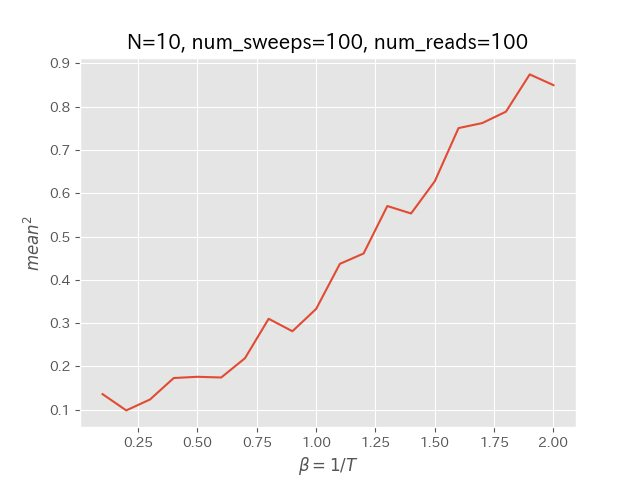
\includegraphics[width=\linewidth]{pictures/2025/01/20250131_085534_001.jpg}
\end{minipage}
\hfill
\begin{minipage}{0.48\linewidth}
\centering
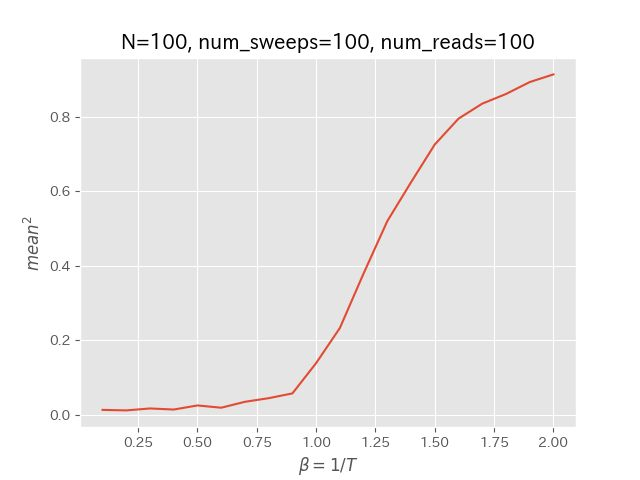
\includegraphics[width=\linewidth]{pictures/2025/01/20250131_085534_002.jpg}
\end{minipage}
\end{center}

\begin{center}
\begin{minipage}{0.48\linewidth}
\centering
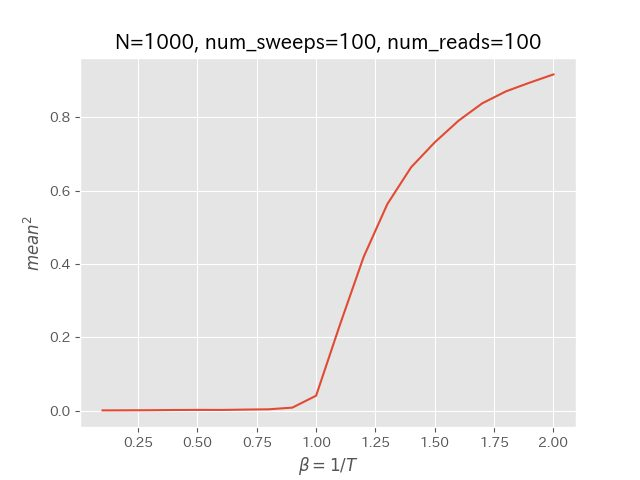
\includegraphics[width=\linewidth]{pictures/2025/01/20250131_085534_003.jpg}
\end{minipage}
\hfill
\begin{minipage}{0.48\linewidth}
\centering
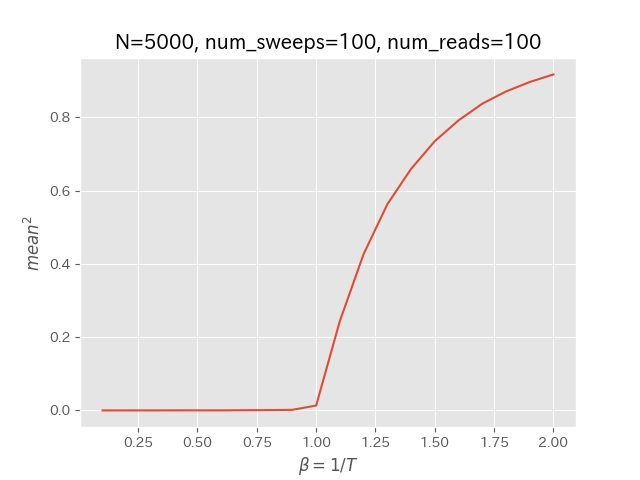
\includegraphics[width=\linewidth]{pictures/2025/01/20250131_085534_004.jpg}
\end{minipage}
\end{center}

\section{2月}

\subsection*{2025年02月01日 14:22}
\addcontentsline{toc}{subsection}{2025年02月01日 14:22}

2025年2月1日

添付の写真は、兼六園の梅林の中できょう最も蕾が膨らんでいたもの。

まだちょっと早いみたいです。（が、明日になったら開いているかな、どうかな。水曜日以降再び強い寒気が来るとの事ですから、、どうでしょう。）

右端の上を向いてる蕾はかなり膨らんでいる様子です。

梅の開花宣言とか梅前線ってあるのかな？

（絞り、もうちょっと絞れたらよかったんだけど、手持ち撮影なので）


\#金沢 \#兼六園 \#梅林

\paragraph{写真}
\begin{center}
\begin{minipage}{0.48\linewidth}
\centering
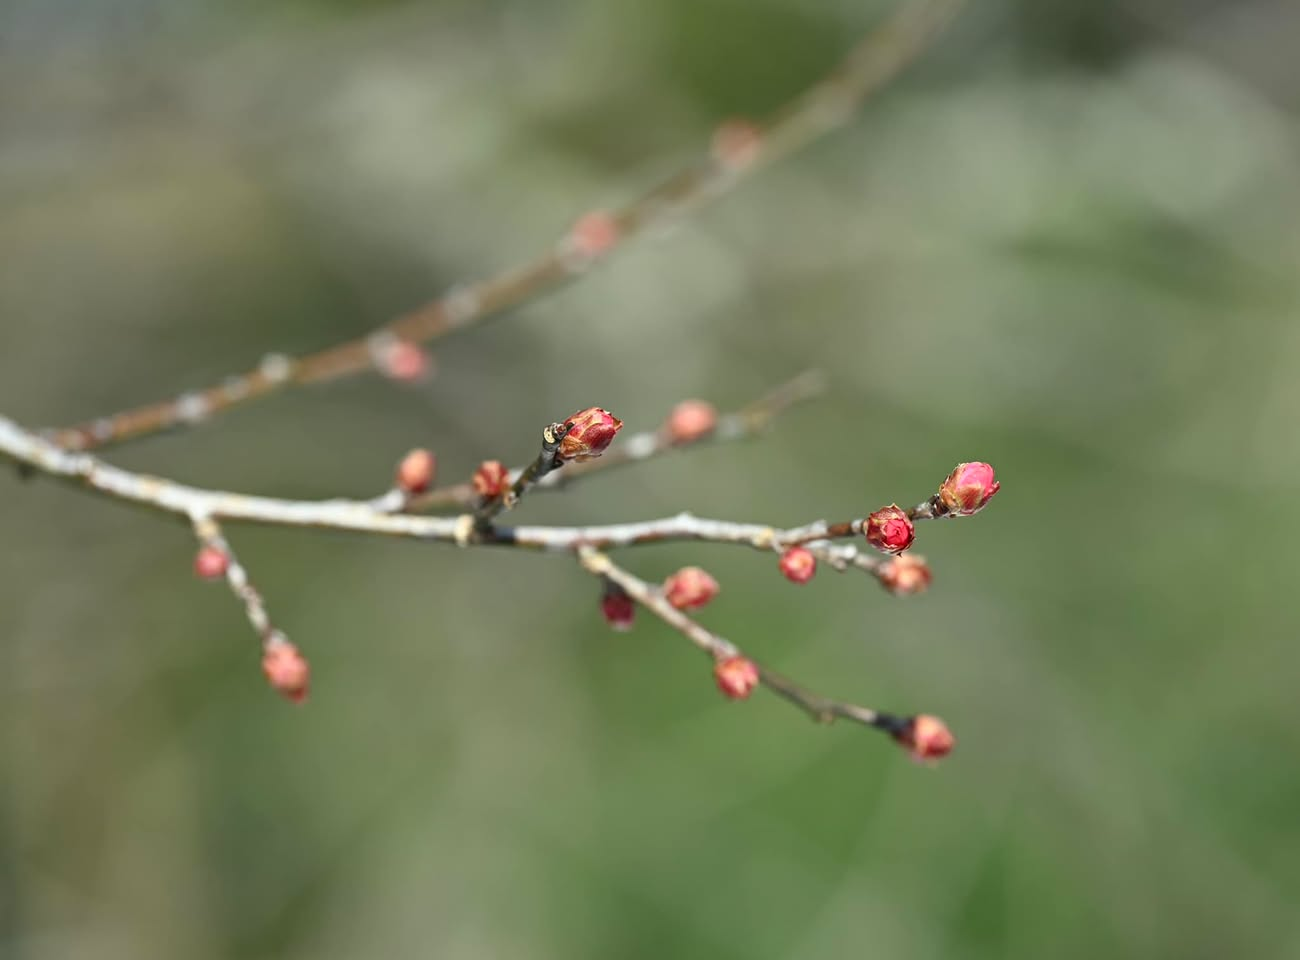
\includegraphics[width=\linewidth]{pictures/2025/02/20250201_142257_001.jpg}
\end{minipage}
\end{center}

\subsection*{2025年02月09日 10:07}
\addcontentsline{toc}{subsection}{2025年02月09日 10:07}

量子コンピュータ（

\url{https://cloud.dwavesys.com/leap/login?next=/leap}

）の無料トライアル期間が1月いっぱいで切れて、\#QA4U3 （

\url{https://altema.is.tohoku.ac.jp/QA4U3/}

）のお勉強に支障有りだったのですが（英語のサイトにもめげずに読んでいくと）GitHubリポジトリのリンクを提供すれば、free trialが毎月自動的に更新されると書かれている様だったので、以前作ったApple Watchで英単語の学習をするアプリを置いていたGitHubのripoを提供してみた所、

additional free time each month on the Leap solvers

をGetできた！みたいです。めでたしめでたし。


（その後）ぬか喜びでした。

API-tokenというものがプログラムする際に必要になるのですが、D-Waveサイトの何処を見ても見つからない？？と思ったら、どうも無料Trialのサービスをやめたらしい事が判明！取り敢えずは、QA4Uのプロジェクトで用意された共用API-tokenを使わせてもらうことになった。ただ、使えるQPU（量子コンピュータでCPUやGPUに相当するもの）時間に限りがあるので、available な時間が無くなったら再びシミュレータを使うことになるのかな。


\#量子コンピュータ \#QPU \#QA4U \#GitHub \#DWave

\paragraph{写真}
\begin{center}
\begin{minipage}{0.48\linewidth}
\centering
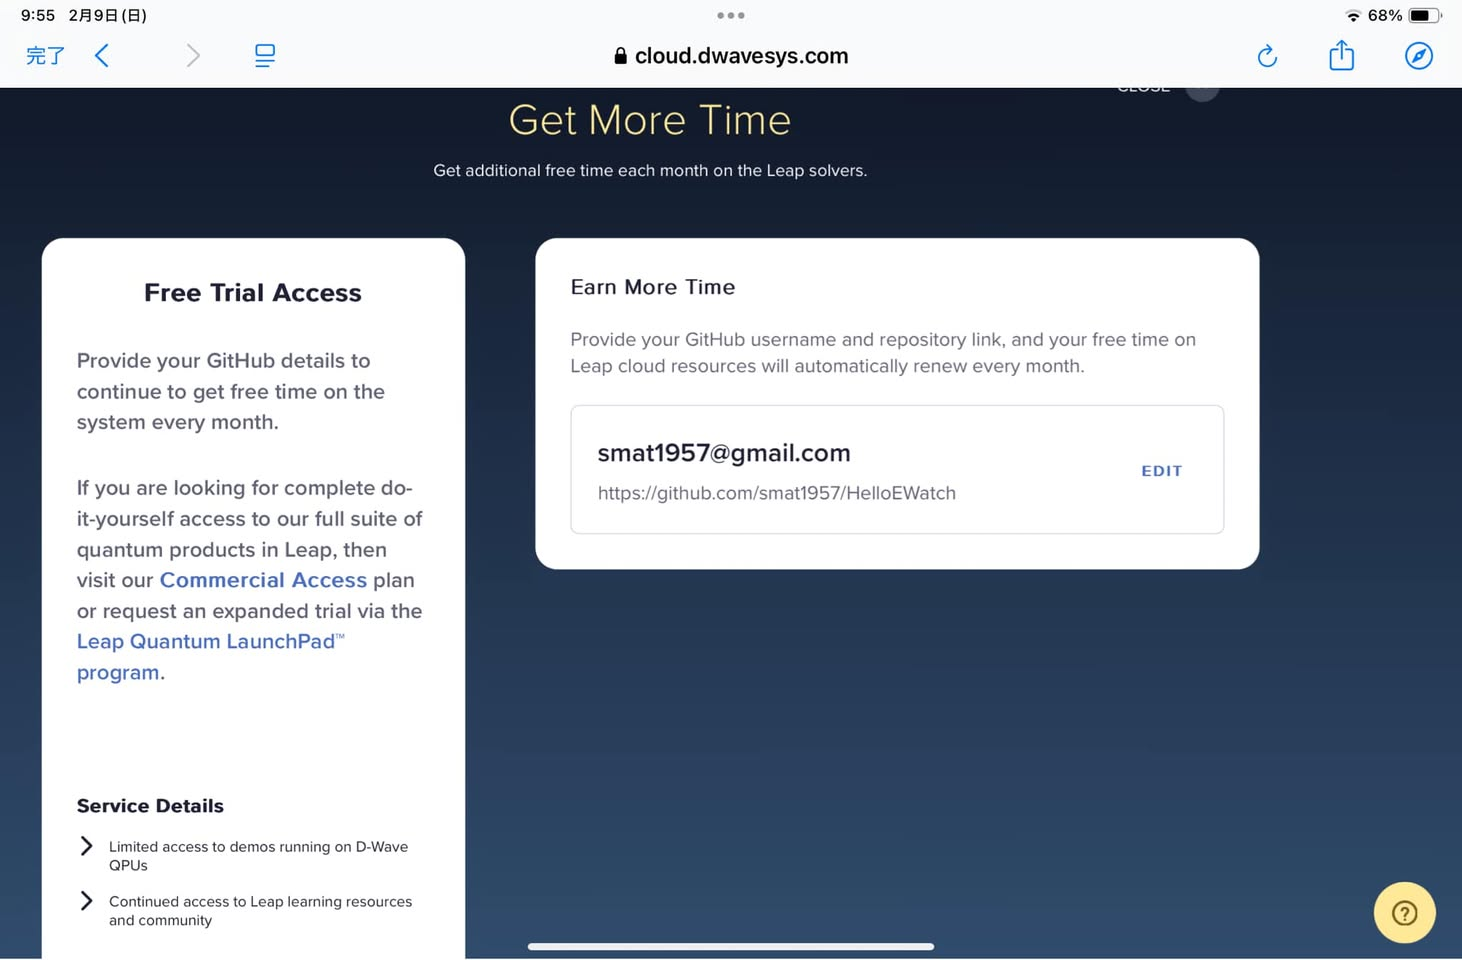
\includegraphics[width=\linewidth]{pictures/2025/02/20250209_100710_001.jpg}
\end{minipage}
\end{center}

\subsection*{2025年02月11日 02:47}
\addcontentsline{toc}{subsection}{2025年02月11日 02:47}

2023年10月23日に、日本のJT-60SAで1stプラズマのnews


\url{https://youtu.be/nbycLI1YjRg}

\begin{center}
\href{https://youtu.be/nbycLI1YjRg}{

\includegraphics[width=0.48\linewidth]{pictures/youtube/2025/02/20250211_024726_youtube_001_nbycLI1YjRg.jpg}
}
\end{center}



\url{https://youtu.be/UFJf39AuxmE}

\begin{center}
\href{https://youtu.be/UFJf39AuxmE}{
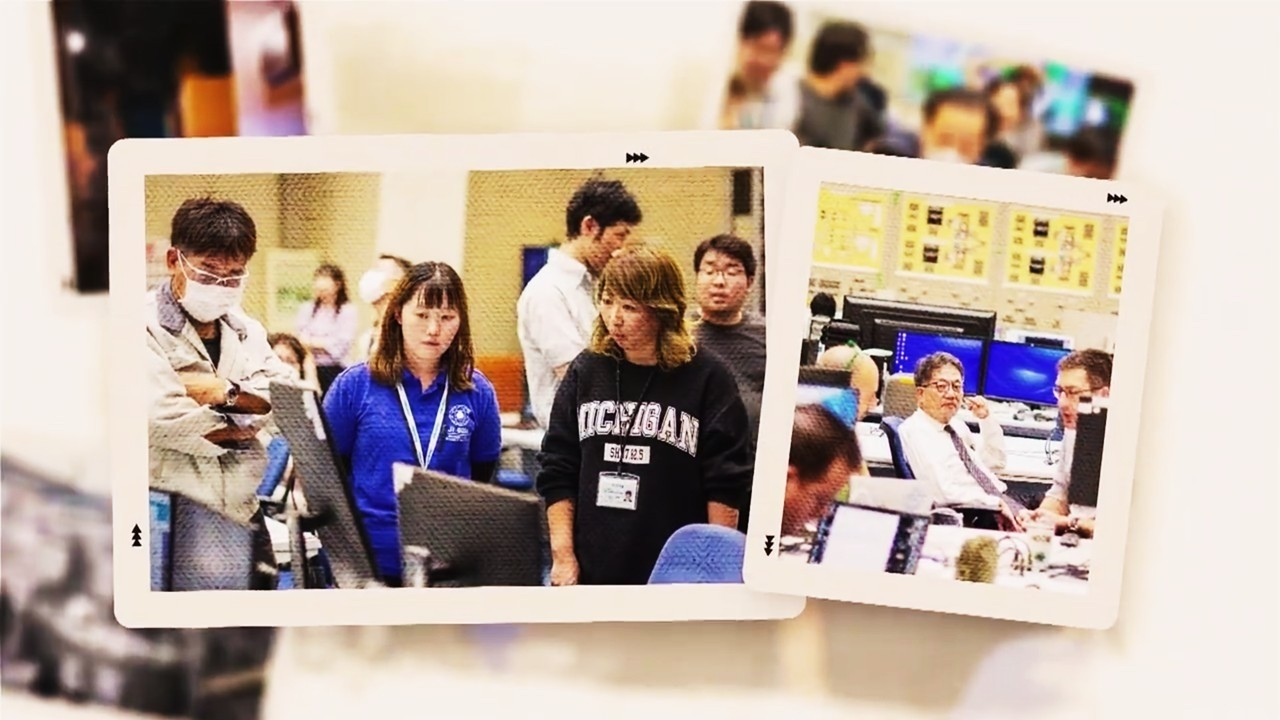
\includegraphics[width=0.48\linewidth]{pictures/youtube/2025/02/20250211_024726_youtube_002_UFJf39AuxmE.jpg}
}
\end{center}




めでたい事です。一方、中国🇨🇳やフランス🇫🇷が比較的長時間のプラズマの維持に成功したというニュースも聞こえてきています。日本の核融合はどんなレベルなんだろう。期待したいと思います。（せめてヤカン一杯の水の沸騰程度でも見てみたいものです）ただ、自分の生きている間に発電が実現される可能性は低い（限りなくゼロに近い）のだろうな、という認識ではいるけれども。


===

この記事は以下の話題の続きです

\url{https://m.facebook.com/story.php?story_fbid=592861772626044&id=100057066806032}



\paragraph{写真}
\begin{center}
\begin{minipage}{0.48\linewidth}
\centering
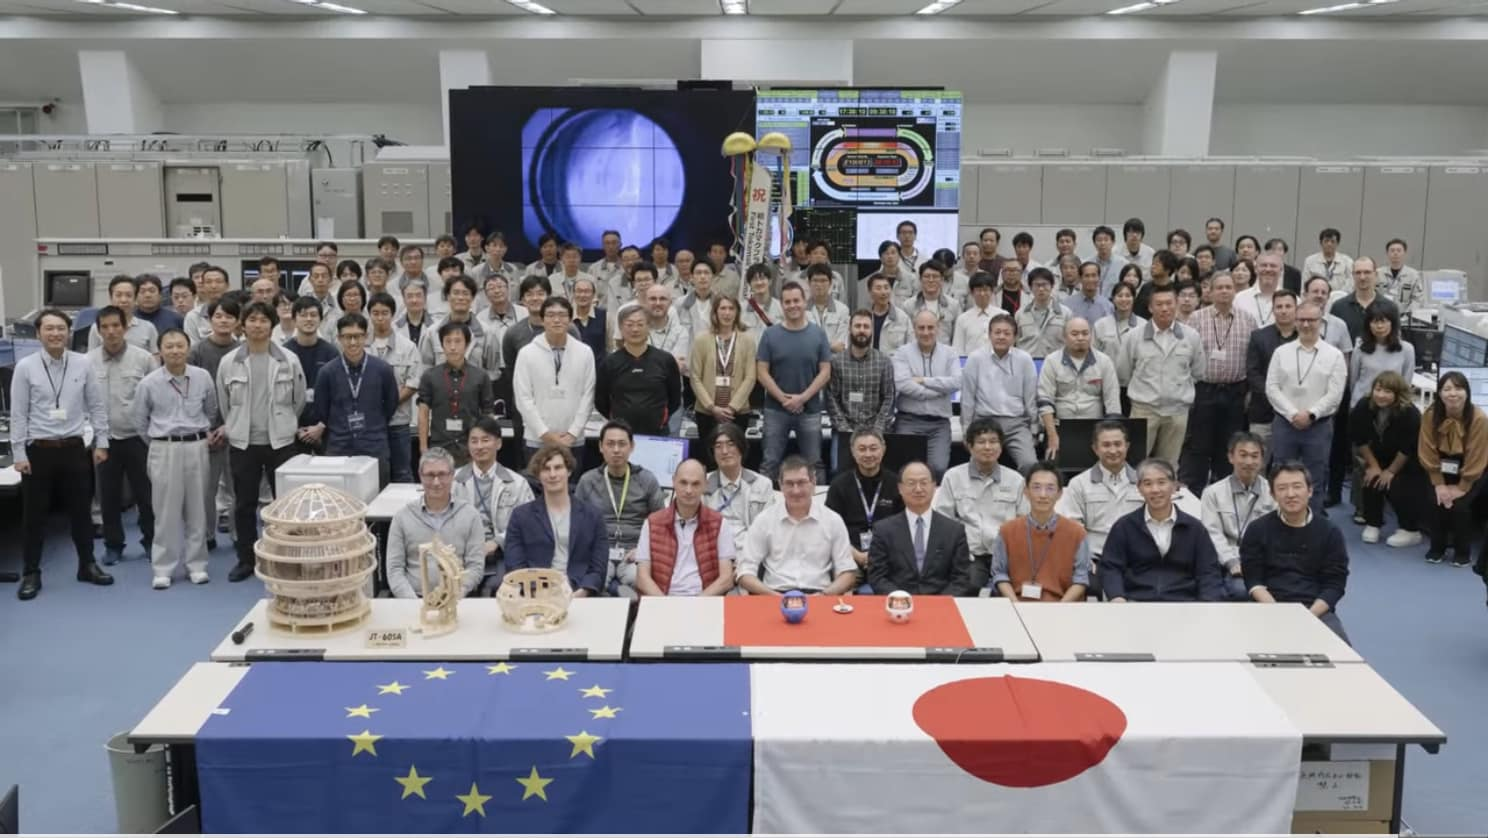
\includegraphics[width=\linewidth]{pictures/2025/02/20250211_024726_001.jpg}
\end{minipage}
\hfill
\begin{minipage}{0.48\linewidth}
\centering
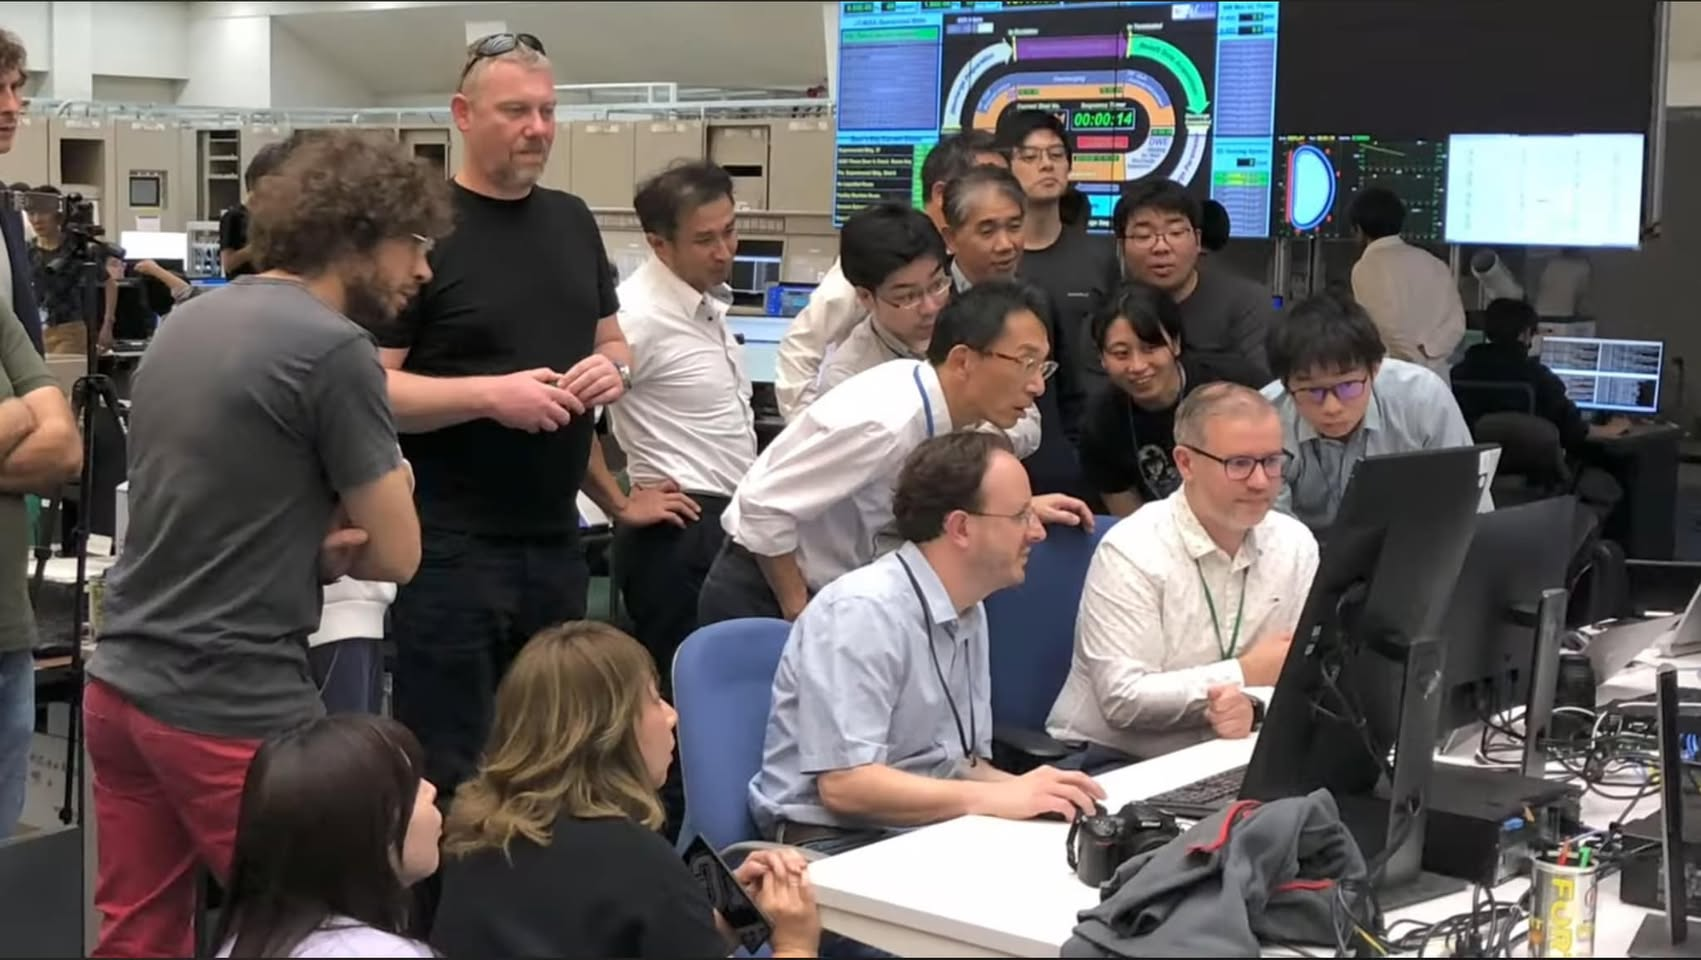
\includegraphics[width=\linewidth]{pictures/2025/02/20250211_024726_002.jpg}
\end{minipage}
\end{center}

\begin{center}
\begin{minipage}{0.48\linewidth}
\centering
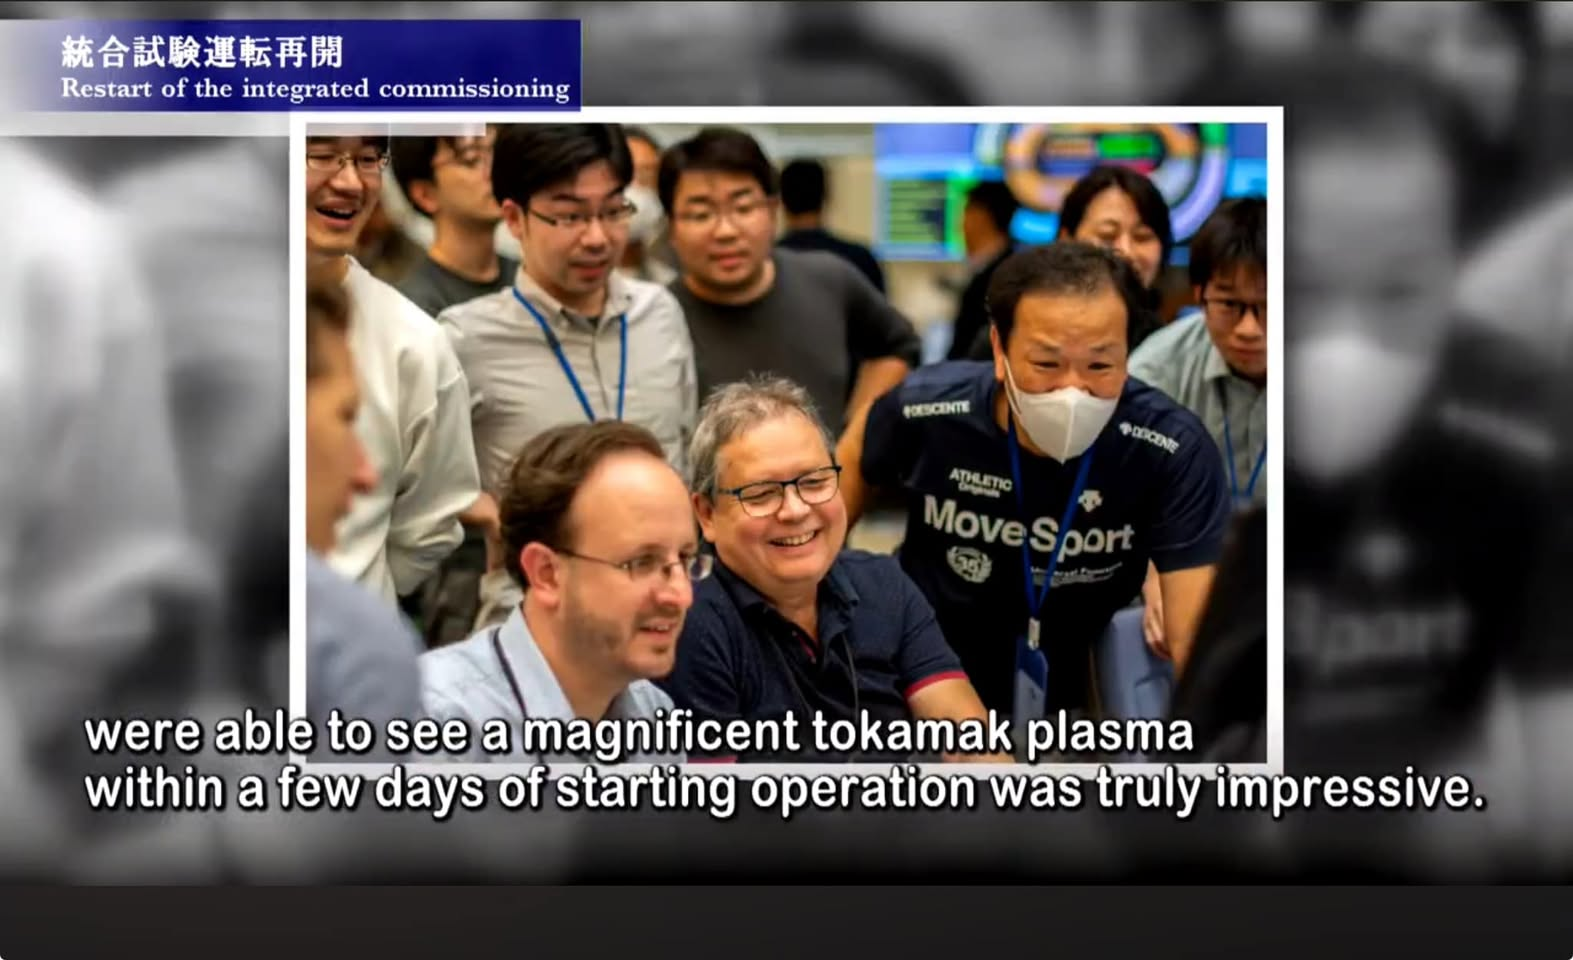
\includegraphics[width=\linewidth]{pictures/2025/02/20250211_024726_003.jpg}
\end{minipage}
\end{center}

\subsection*{2025年02月11日 23:00}
\addcontentsline{toc}{subsection}{2025年02月11日 23:00}

\#量子コンピュータ のプログラムを試せるという \#QA4U3 プロジェクト（

\url{https://altema.is.tohoku.ac.jp/QA4U3/}

）で、第二回（

\url{https://youtu.be/yzsSsS7Mq0g}

\begin{center}
\href{https://youtu.be/yzsSsS7Mq0g}{

\includegraphics[width=0.48\linewidth]{pictures/youtube/2025/02/20250211_230044_youtube_001_yzsSsS7Mq0g.jpg}
}
\end{center}

） の講義を受講した（2月7日）


2024年に \#ノーベル物理学賞 を受賞された \#ホップフィールド さんと \#ヒントン さんの業績を、\#ホップフィールドネットワーク と \#ボルツマンマシン を \#Python でプログラムして、\#量子アニーリングマシン で実行する事で追体験する事ができた。


ホップフィールドさんのモデルでは、既知のデータを \#相互作用 の行列に記憶させて、それを量子アニーリングマシンにかけると、元のデータを「想起」できる事を確認した。奇妙な事に、相互作用の行列に記憶させるのは1つのデータじゃないという事です。複数のデータを足し合わせているだけなのに、、不思議だ。


ヒントンさんのボルツマンマシンでは、全くランダムな（無秩序な）状態のデータからスタートして、既知のデータとの差を使って相互作用の行列を更新しては、それを量子アニーリング（QA）コンピュータに渡して結果を受け取り、その結果を再度既知データと比較して相互作用の行列を更新してQAコンピュータに渡し、という事をを繰り返していくと、だんだん既知のデータに似た秩序ある構造に似たものを出力する様になってくる。既知のデータを出力する様な相互作用の行列が最終的にできあがる。これは既知のデータを元に「学習」した事になるという事なのですが、スタートが全くランダム（無秩序）なのに、、これまた不思議です。


添付はボルツマンマシンで、全く無秩序な状態から「学習」を進めて、構造を獲得していく途中段階の出力。初めの3行分の画像はスタート時のランダムな様子。もう１つの画像の3行は50回の更新をした辺りの様子。手書き数字文字の３と５？が現れてきている様に見える。


この実験では8x8で各画素が16階調のデータ（\#MNIST と呼ばれる手書き数字文字データセット）を使っているが、もっと大きなデータで実験すれば、（\#イジングモデル の時の様に、ある時点で \#相転移 を起こして急激に）クリアな結果にたどり着くのかもしれない。（人の顔写真でもやってみたいものだ。）

\paragraph{写真}
\begin{center}
\begin{minipage}{0.48\linewidth}
\centering
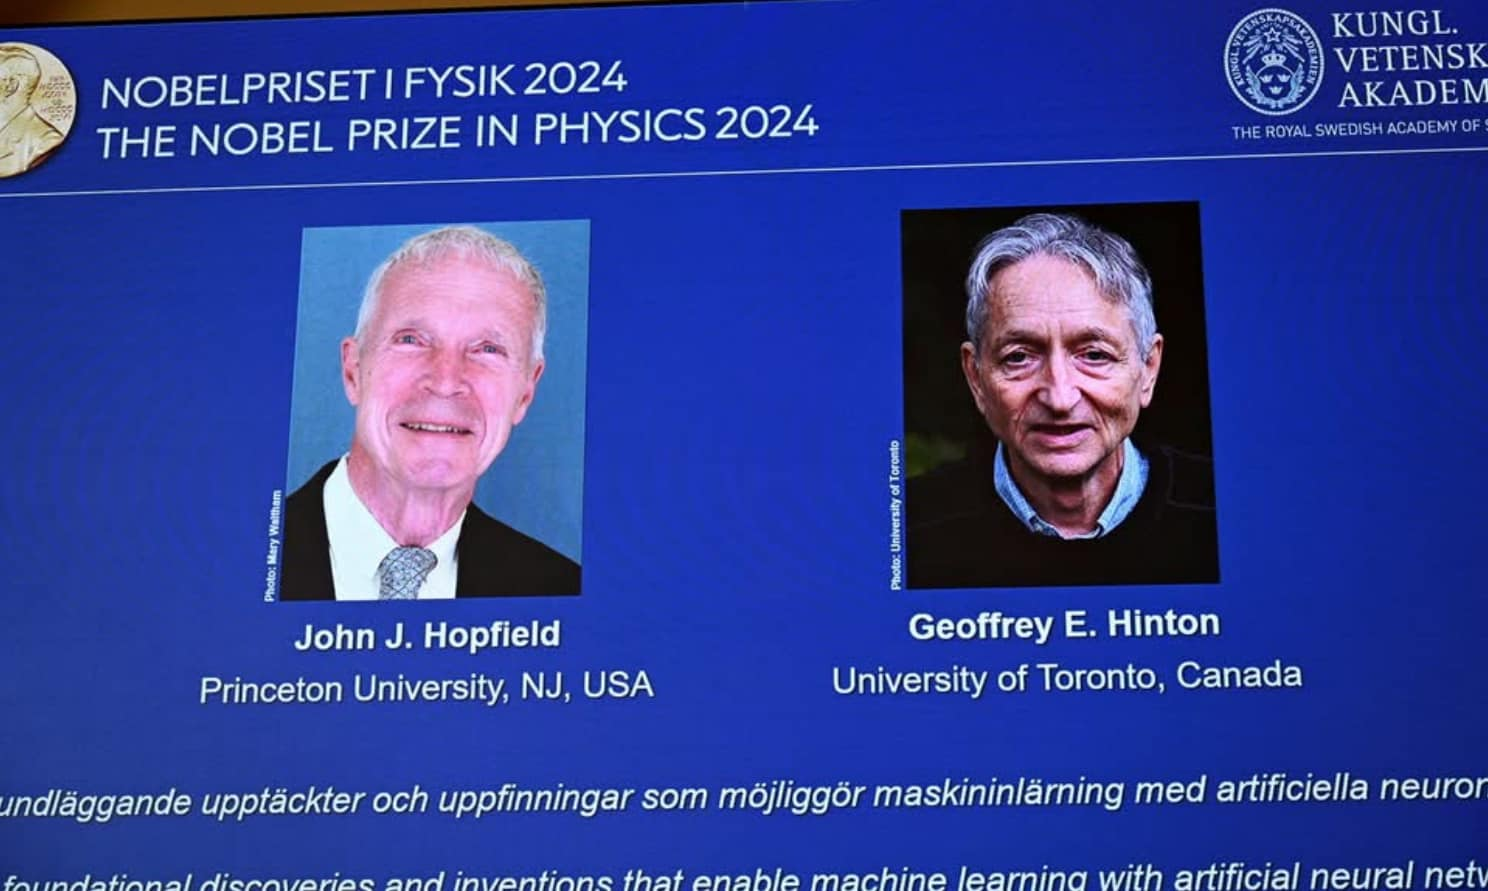
\includegraphics[width=\linewidth]{pictures/2025/02/20250211_230044_001.jpg}
\end{minipage}
\hfill
\begin{minipage}{0.48\linewidth}
\centering
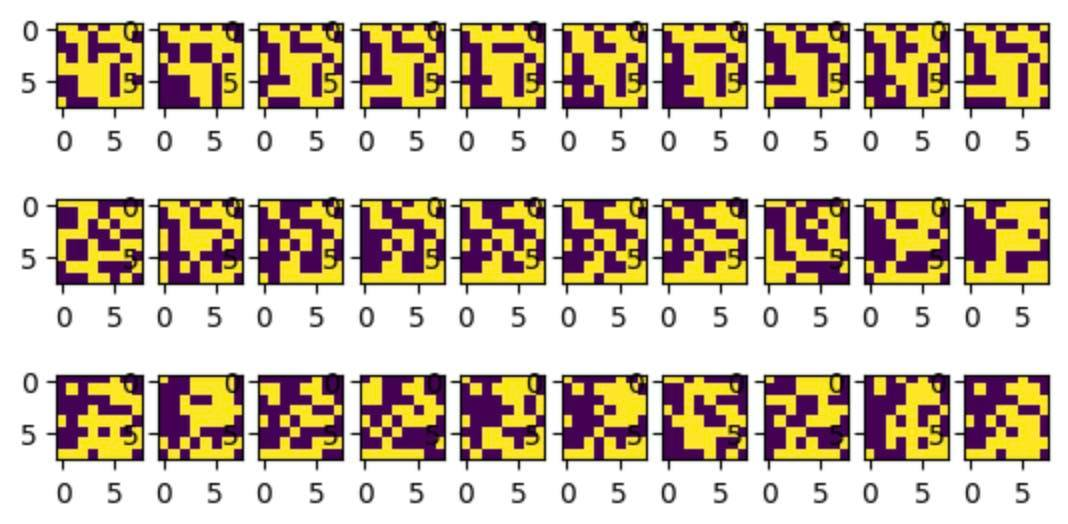
\includegraphics[width=\linewidth]{pictures/2025/02/20250211_230044_002.jpg}
\end{minipage}
\end{center}

\begin{center}
\begin{minipage}{0.48\linewidth}
\centering
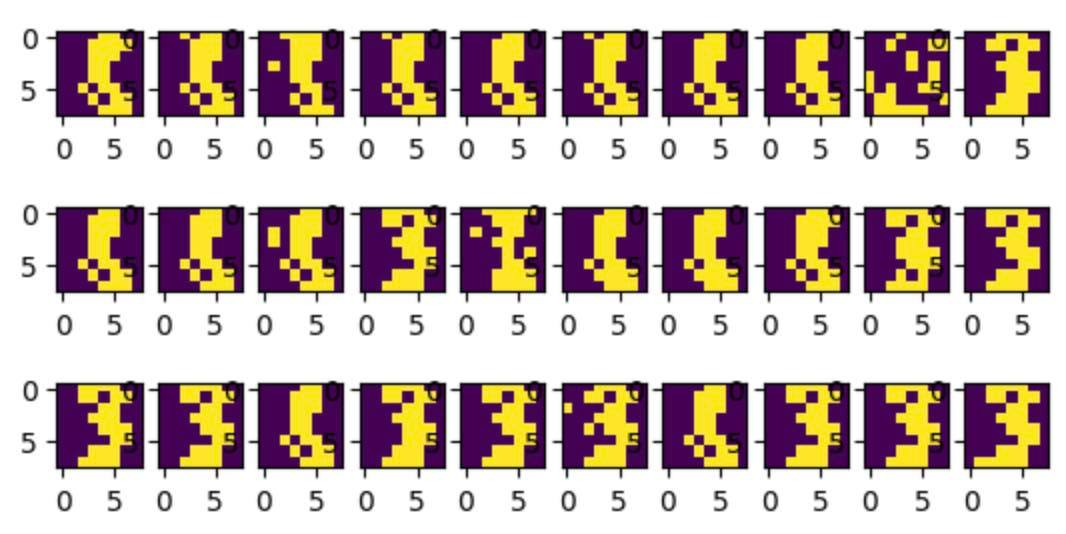
\includegraphics[width=\linewidth]{pictures/2025/02/20250211_230044_003.jpg}
\end{minipage}
\end{center}

\subsection*{2025年02月12日 03:05}
\addcontentsline{toc}{subsection}{2025年02月12日 03:05}

BWV147（主よ人の望みの喜びよ）のギター編について


佐藤弘和氏の解説（ 

\url{https://music-bells.com/?pid=43985853}

 ）によれば、

===引用開始

J.S.バッハのカンタータ第147番“心と口と行いと生活で”(BWV147)（全10曲）は２部に分かれ、それぞれがこの有名な「主よ人の望みの喜びよ」で終わるようになっています。タイトルは英訳の通称ですが、原曲では第６曲「イエスこそわが喜び」、第10曲「イエスは変わらざるわが喜び」と、違う歌詞で歌われます。

===引用終わり

ふーむ、そうだったのか


原曲はG-dur

多くのギター編はG-durのまま編曲されている（コメント欄にあげたものは全てG-dur ）

それにしても、こんなに色々な方のそれぞれが編曲に取り組まれているというのは、いったい何故なんでしょうか？決定版の編曲というものが無い状態なのか？この曲自体がそもそも編曲に取り組み易い曲なのか？他の人の編曲では満足できないという状況になっているのかな？


これ↓は 林 祥太郎 氏の編曲で、ご自身による演奏です（ジュリアン・ブリームの愛用した楽器なのか）

\url{https://youtu.be/0kJ7IffSHvo}

\begin{center}
\href{https://youtu.be/0kJ7IffSHvo}{
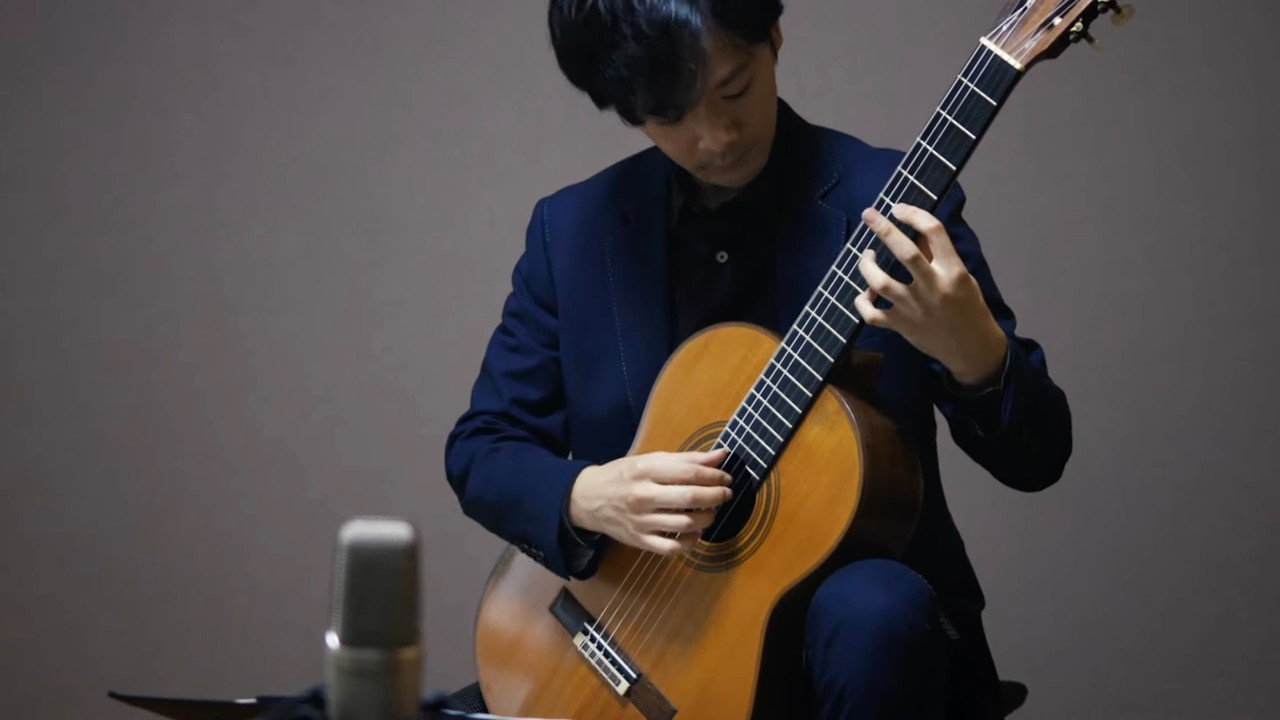
\includegraphics[width=0.48\linewidth]{pictures/youtube/2025/02/20250212_030510_youtube_001_0kJ7IffSHvo.jpg}
}
\end{center}



楽譜はここ↓で購入できる（G-dur、第6弦をDにドロップしなくてもいい＝Eのままでいい）

\url{https://m.mymusicfive.com/shotarohayashi/57772}




一方、G-dur 以外の調に編曲されたものもある（にはある）

佐々木忠編はA-durで、楽譜は（ 

\url{https://www.gendaiguitar.com/products/4511005095558}

 ）第3弦をFis に、との指示になっている

田部井辰雄編はD-durで、楽譜は「田部井辰雄ギターワールド Vol.2」（サーベル社）にあるが、この曲集は今は絶版になっている。実はこの曲集は貴重です カタロニア民謡から鳥の歌の田部井氏による編曲もこれに入っている（ 

\url{https://m.facebook.com/story.php?story_fbid=24514344341556396&id=100002225117991}

 ）


===

バッハのギター曲（の全貌？）はこちら

\url{https://m.facebook.com/story.php?story_fbid=25468465252810962&id=100002225117991}



\subsection*{2025年02月12日 03:05}
\addcontentsline{toc}{subsection}{2025年02月12日 03:05}

\paragraph{リンク}
\url{https://youtu.be/zwzjLeQIokE}

\begin{center}
\href{https://youtu.be/zwzjLeQIokE}{
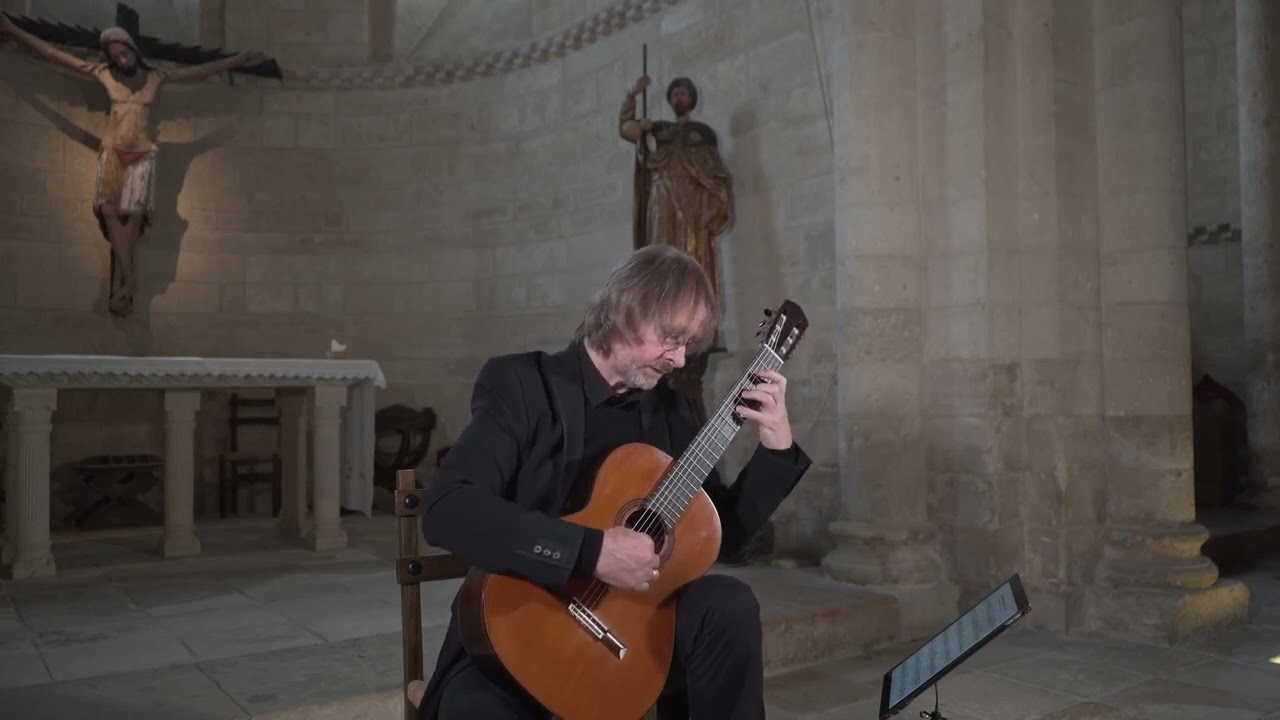
\includegraphics[width=0.48\linewidth]{pictures/youtube/2025/02/20250212_030544_youtube_001_zwzjLeQIokE.jpg}
}
\end{center}

\subsection*{2025年02月12日 03:21}
\addcontentsline{toc}{subsection}{2025年02月12日 03:21}

\paragraph{リンク}
\url{https://youtu.be/EdQZqX6eJ7U}

\begin{center}
\href{https://youtu.be/EdQZqX6eJ7U}{
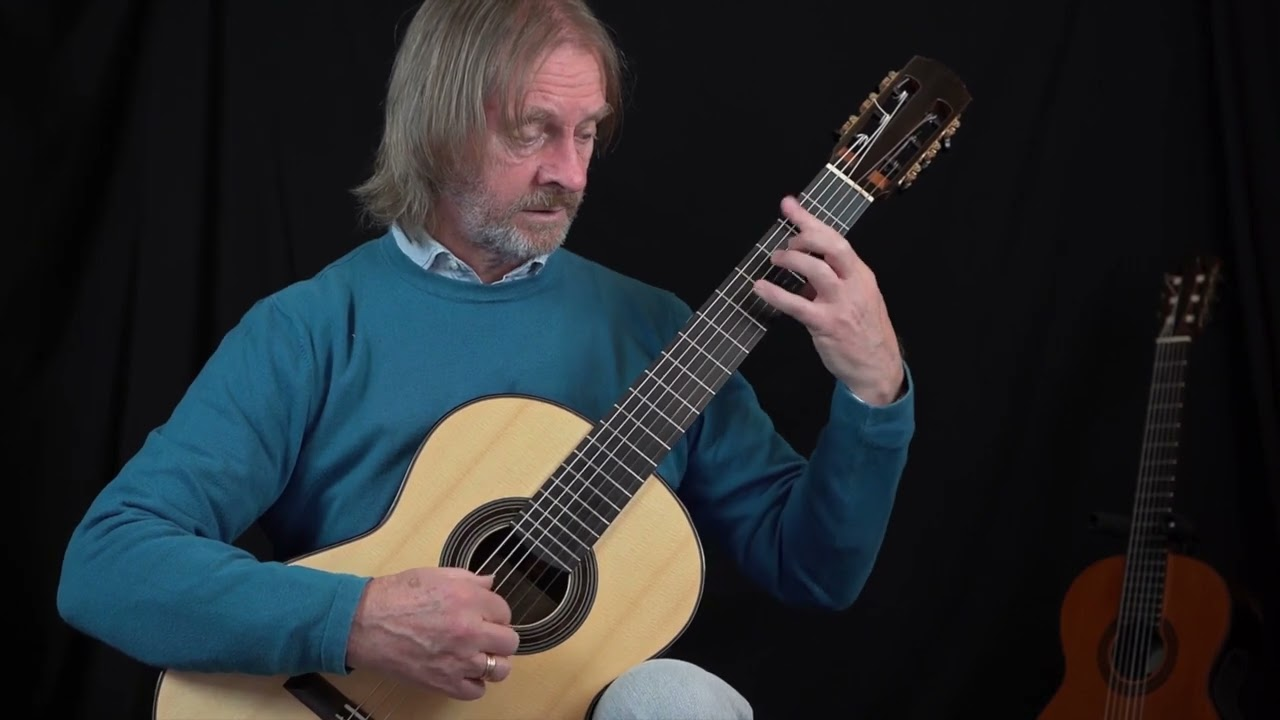
\includegraphics[width=0.48\linewidth]{pictures/youtube/2025/02/20250212_032110_youtube_001_EdQZqX6eJ7U.jpg}
}
\end{center}

\subsection*{2025年02月12日 08:43}
\addcontentsline{toc}{subsection}{2025年02月12日 08:43}

数式を使わないで専門的な内容を語ろうとする本、啓蒙書にありがちなことかと思いますが、読む人によって、「読者が予め知っている知識に依って、理解の度合いは異なる」ものなのだと思います。


高校生の頃にブルーバックスのシリーズにハマっていた事がありました。その頃の知識レベルで読んでいたとは思いますが、大学で専門書を読んでから見返した時に、本の中のこの説明はつまりゲージ変換の事を言っていたのかとか、積分形式で言い直していたんだな等という事があって、ようやく何を言いたいのかが分かったと言う気がした事がありました。


添付の本は \#岩波書店 の「 \#生成AIのしくみ 」ですが、イジングモデルやボルツマンマシンについても解説されています。そして2人のノーベル物理学賞受賞者に関しては、コラム記事の格好で載っています。\#QA4U3 でお勉強した甲斐あって、内容がよりよく分かった様な気がします。もっと言えば、QA4U3のお勉強をする前の状態では、そもそも受賞された2人の物理学者が貢献された事柄の間の違いも理解していなかったわけですから、この本の内容を十分に分かって（読めて）いなかったのは明らかです。

また、この本によれば、QA4U3で学習している事より、もっともっと先があるんだという事も分かります。その部分については読み物レベルの理解にしかなっていないのだろうと思います。

\paragraph{写真}
\begin{center}
\begin{minipage}{0.48\linewidth}
\centering
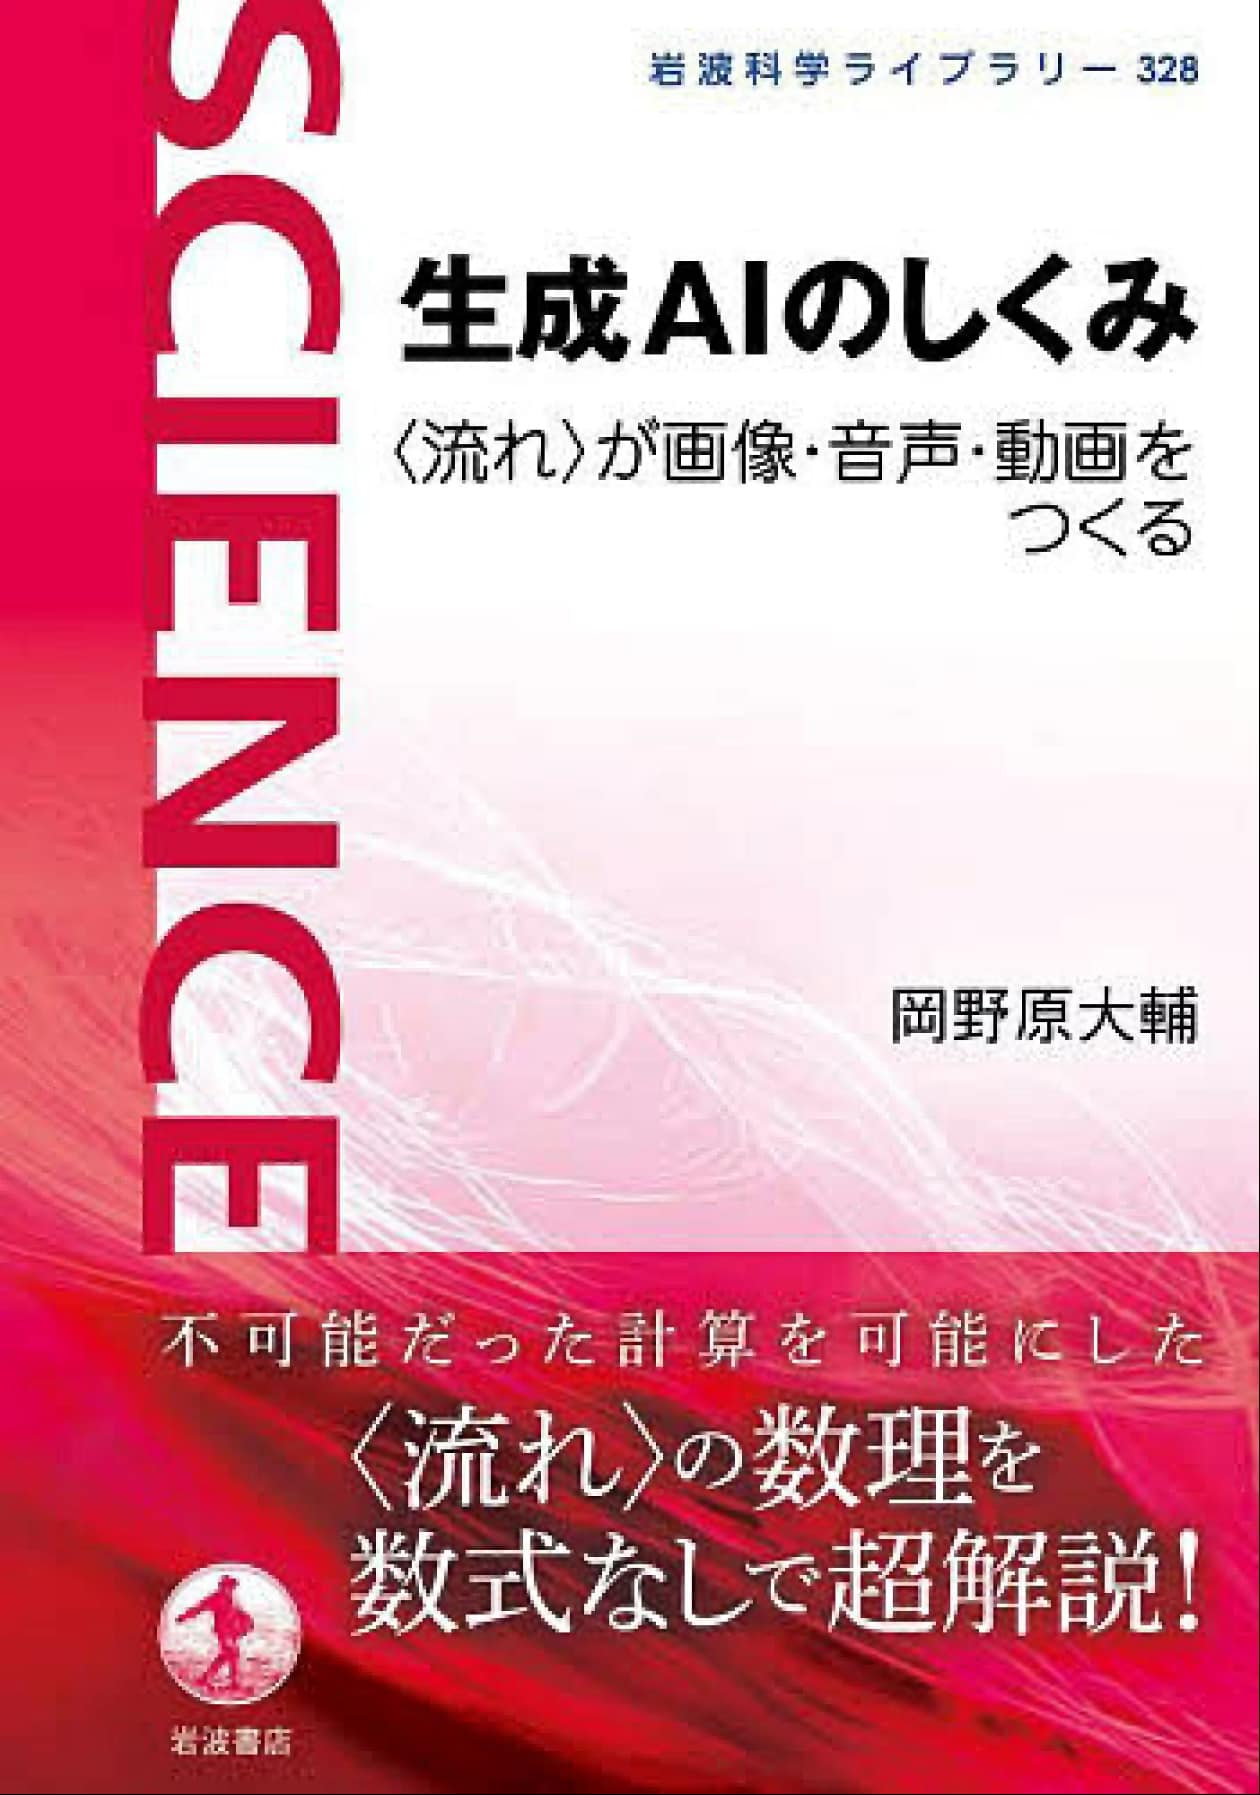
\includegraphics[width=\linewidth]{pictures/2025/02/20250212_084303_001.jpg}
\end{minipage}
\end{center}

\subsection*{2025年02月13日 22:52}
\addcontentsline{toc}{subsection}{2025年02月13日 22:52}

HopfieldネットワークをOpenjijシミュレータで動かすプログラムを作ってみた。サンプラーにはSASampler()を使っている。


添付の上の段の2枚の画像は、手書き数字文字データセットから無作為に選んだ2枚です。この2枚のデータを元にして相互作用のJ行列を作り、量子アニーリングコンピュータ（のシミュレータ）に渡し、その結果をnum\_reads=10回読んで、それを画像にしたのが下の段の10枚です。


\#ホップフィールドネットワーク \#シミュレータ \#Python \#QA4U3

\paragraph{写真}
\begin{center}
\begin{minipage}{0.48\linewidth}
\centering
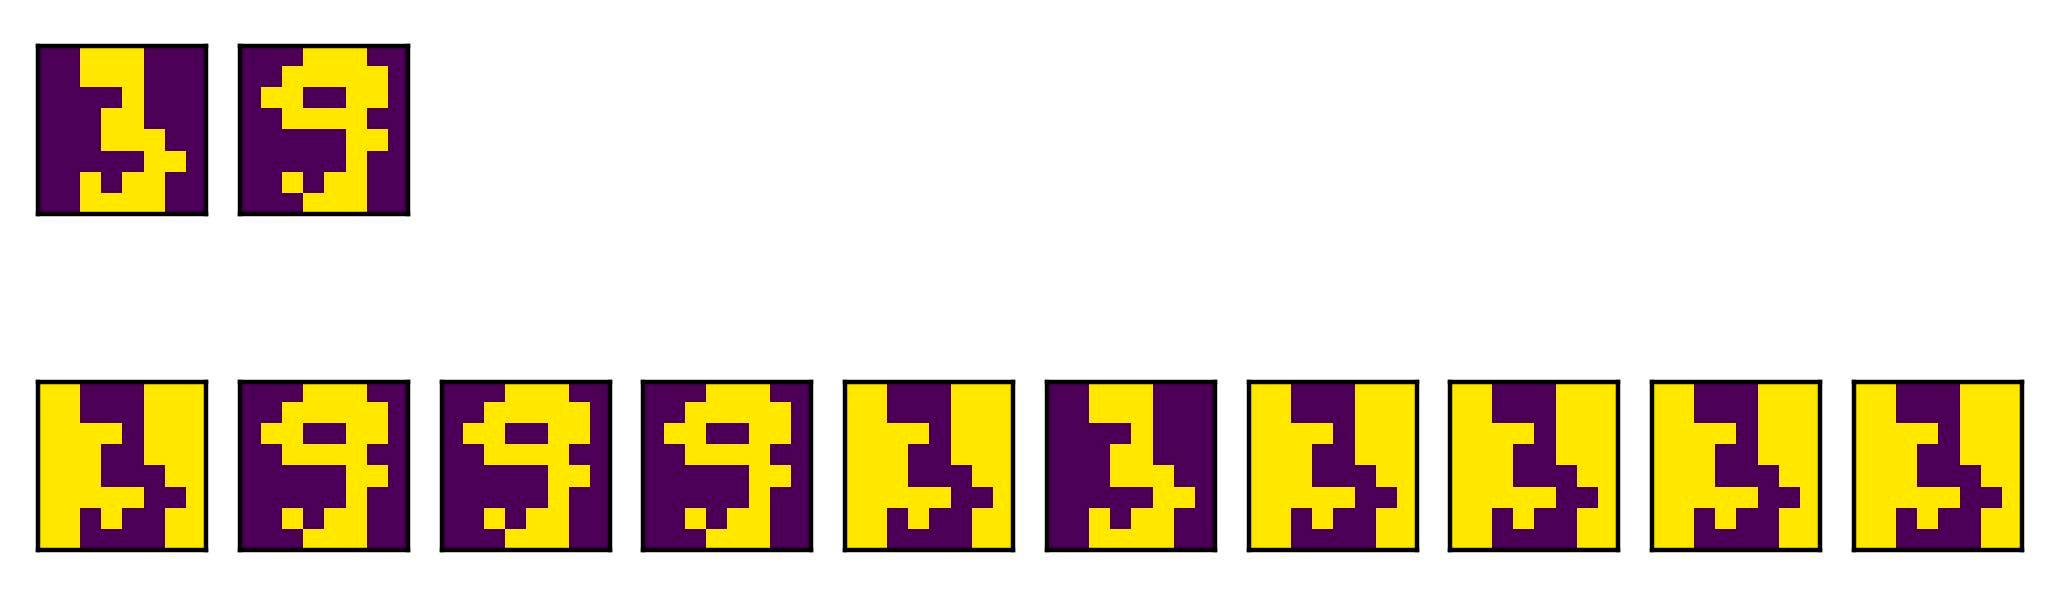
\includegraphics[width=\linewidth]{pictures/2025/02/20250213_225259_001.jpg}
\end{minipage}
\end{center}

\subsection*{2025年02月13日 22:54}
\addcontentsline{toc}{subsection}{2025年02月13日 22:54}

ボルツマンマシンをOpenjijシミュレータで動かすプログラムを作ってみた。サンプラーにはSQASampler()を使っている。


最上段の4枚の画像は、手書き数字文字データセットから無作為に選んだ4枚で、この4枚からデータのqubo行列を作っています。

2行目以降は、量子コンピュータ（のシミュレータ）からnum\_reads=10回読み出したσiとσjを画像にしたものです。量子コンピュータ（のシミュレータ）が出力する10枚の画像と4枚の元の画像データの差でqubo 行列を更新しては量子コンピュータ（のシミュレータ）に渡しています。5回の更新毎にスナップショットとしてnum\_reads=10枚（1行）を表示しているので、一番下の行は50回更新した時の量子コンピュータ（のシミュレータ）からの出力を描いたものになります。


最初全くランダムで無秩序な状態だったもの（2行目の10枚）が、50回の更新によって、元データ（1行目の4枚）の構造に似たものを見せてくる（最終行の10枚）のはとても面白いと思います。


\#ボルツマンマシン \#シミュレータ \#Python \#QA4U3

\paragraph{写真}
\begin{center}
\begin{minipage}{0.48\linewidth}
\centering
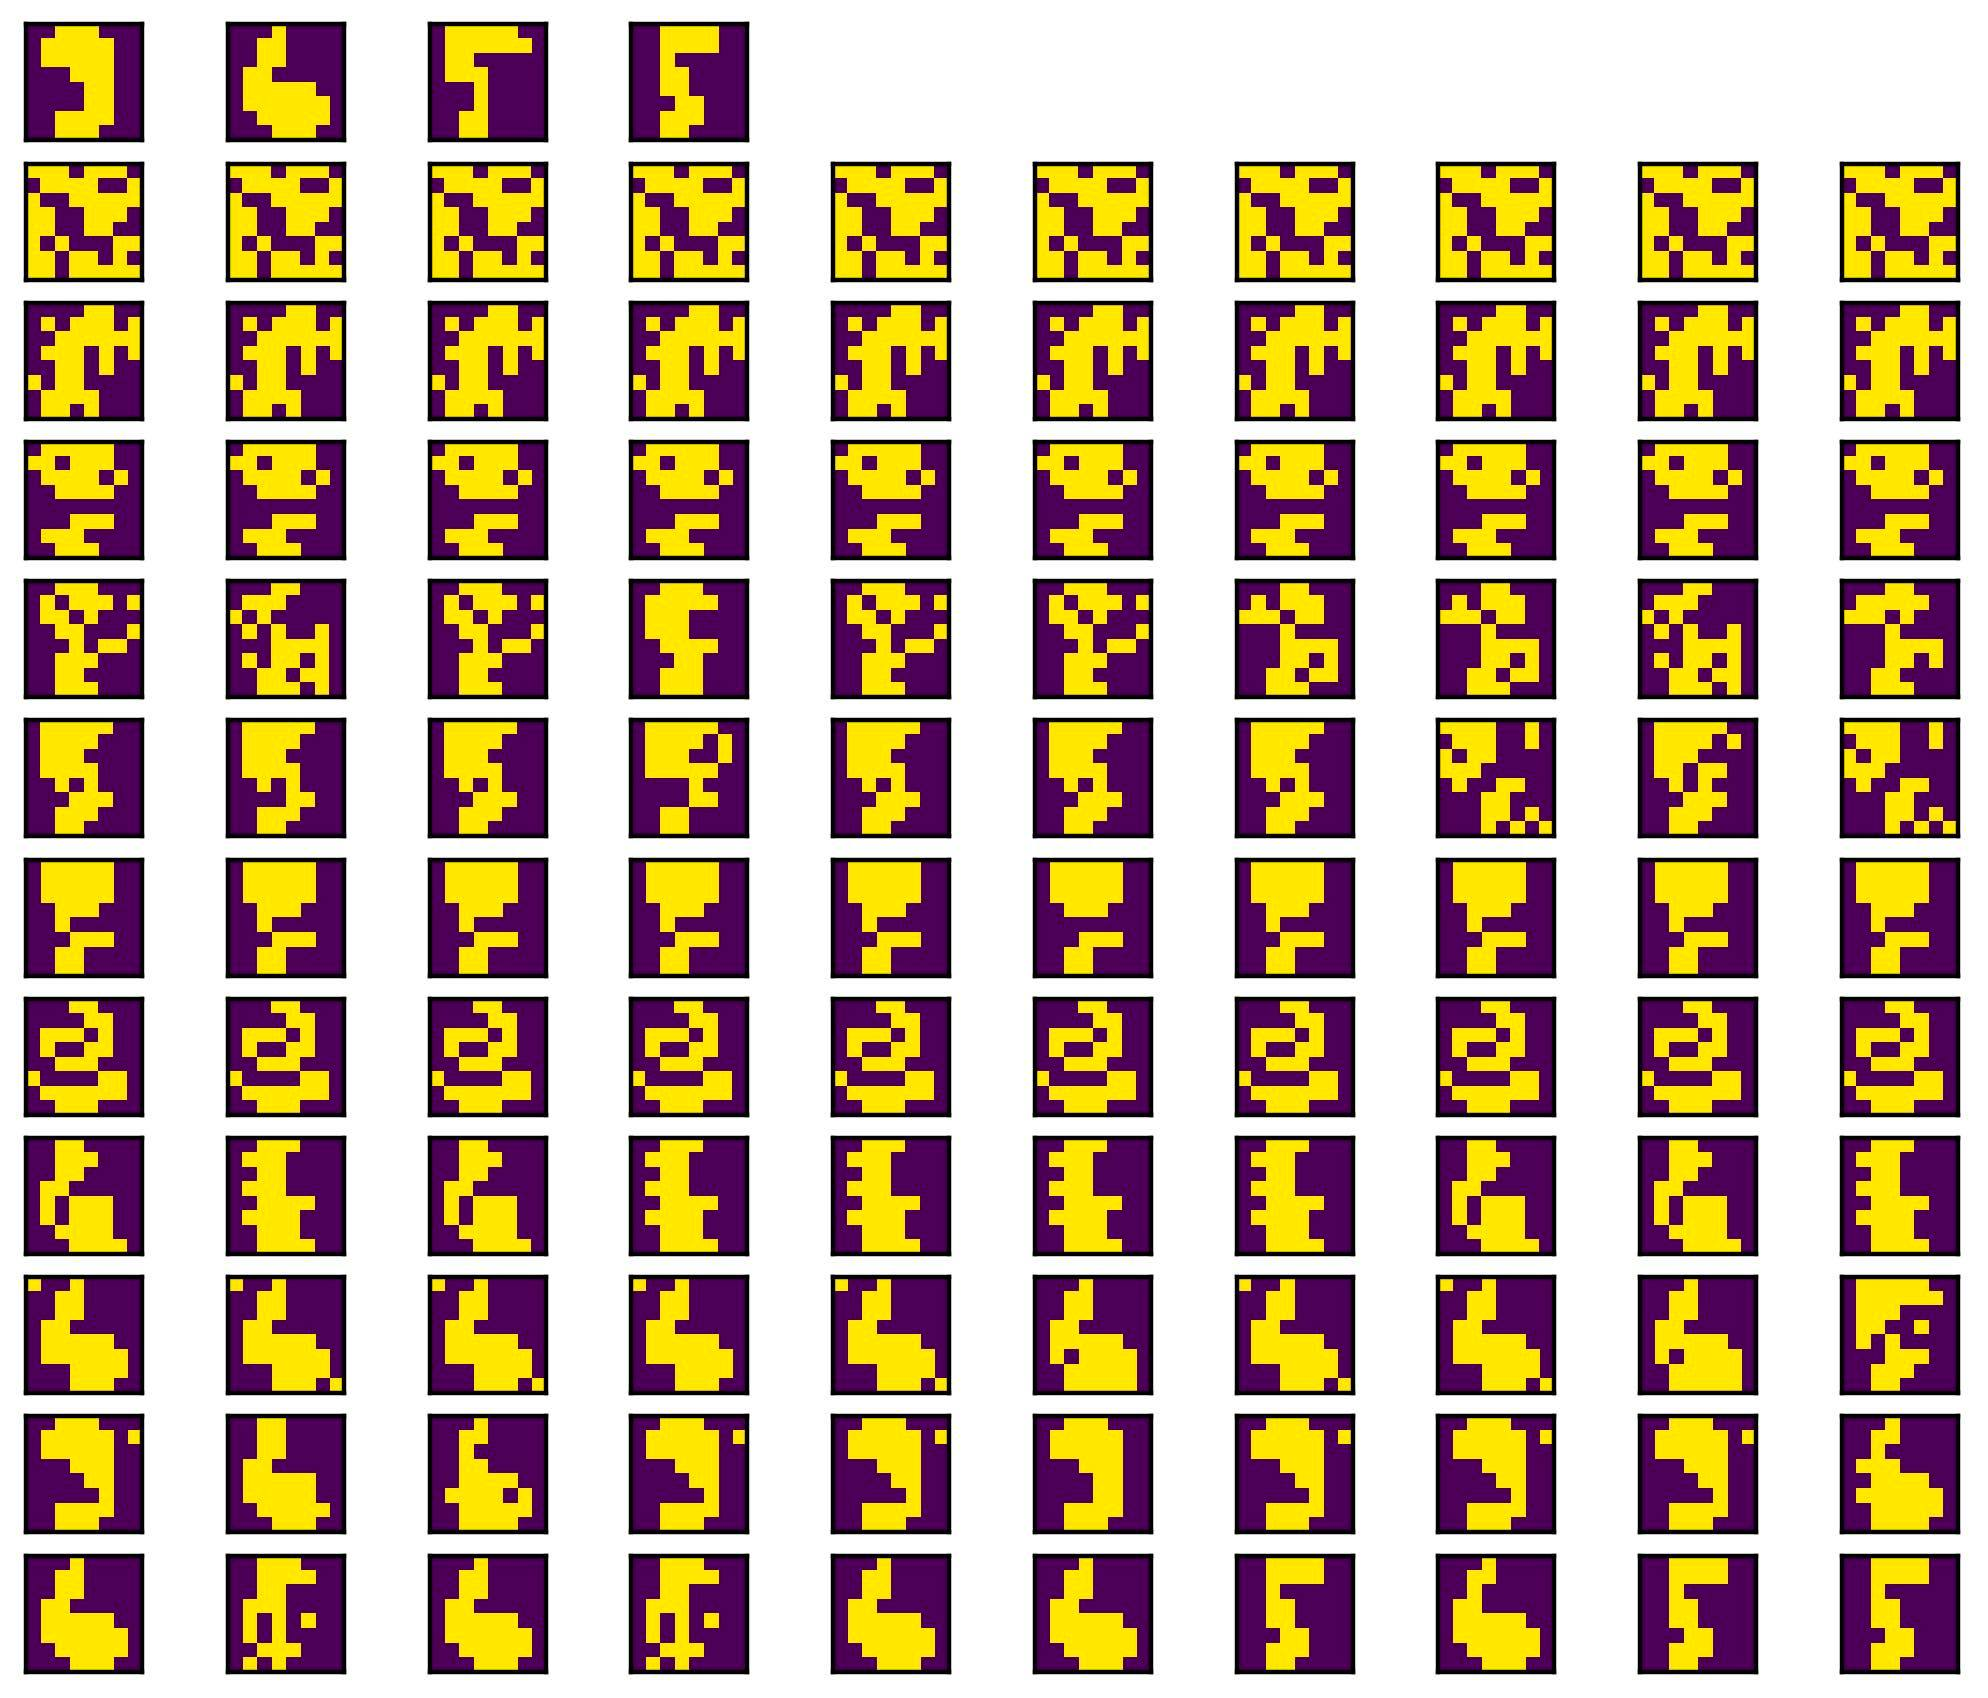
\includegraphics[width=\linewidth]{pictures/2025/02/20250213_225420_001.jpg}
\end{minipage}
\end{center}

\subsection*{2025年02月14日 21:44}
\addcontentsline{toc}{subsection}{2025年02月14日 21:44}

\paragraph{リンク}
\url{https://tutorial.openjij.org/build/html/ja/001-Introduction.html}

\subsection*{2025年02月15日 08:28}
\addcontentsline{toc}{subsection}{2025年02月15日 08:28}

\#量子コンピュータ のプログラムを試せるという \#QA4U3 プロジェクト（

\url{https://altema.is.tohoku.ac.jp/QA4U3/}

）で、第三回（

\url{https://youtu.be/7rVJ_8Q1km0}

\begin{center}
\href{https://youtu.be/7rVJ_8Q1km0}{

\includegraphics[width=0.48\linewidth]{pictures/youtube/2025/02/20250215_082808_youtube_001_7rVJ_8Q1km0.jpg}
}
\end{center}

）の講義を受講する予定です。（2月15日17時スタート）

前回（第二回）は画像を生成しましたが、今回（第三回）は時系列データの生成がテーマという事の様ですので、量子コンピュータに作曲させることになるらしい。楽しみです。

\subsection*{2025年02月15日 08:30}
\addcontentsline{toc}{subsection}{2025年02月15日 08:30}

\paragraph{リンク}
\url{https://youtu.be/7rVJ_8Q1km0}

\begin{center}
\href{https://youtu.be/7rVJ_8Q1km0}{

\includegraphics[width=0.48\linewidth]{pictures/youtube/2025/02/20250215_083008_youtube_001_7rVJ_8Q1km0.jpg}
}
\end{center}

\subsection*{2025年02月15日 08:50}
\addcontentsline{toc}{subsection}{2025年02月15日 08:50}

2月15日の朝6時50分頃、西に沈む月です。（地上の街には、まだ朝日がさしていません）この後空が明るくなって、月も薄くなって見えなくなっていきますから、この時が撮影の適時だったと思います。

また、これより広角のレンズだと月が小さくなって月面のディテールが分からなくなります。望遠だと地上が画面に入らない。（より望遠で地上も入れようとすると、月がもっと傾いてから撮る必要があるが、もう朝日で明るくなりかけていて、月も薄くなってきている）このレンズがギリギリ画角を満足する焦点距離だと思います。

今日は貴重な晴れの1日（散歩日和）のはず。明日以降1週間ほどは、また10年に1度の雪だそうですから。（10年に1度の大雪は今季2度目→5年に1度？）


Nikkor Z MC 105mm f2.8 VR Sによる手持ち撮影（レタッチ無しトリミング無しのjpeg撮って出し）です。Nikon製のZマウントレンズで、VRは手ぶれ補正機能付き、MCはマイクロ（等倍接写）対応、Sは高画素機のカメラボディでも使用に耐えるの意味（普通のレンズが持っている各種収差等の欠点は、低画素機では目立たないが、高画素機では顕在化、露呈する）。


今回カメラボディは低画素機ですが、本当によく写っている。このレンズで撮影した写真を見るにつけ、凄いレンズなんだな！といつも思います。（先日撮影した梅の蕾もこのレンズでした）

\paragraph{写真}
\begin{center}
\begin{minipage}{0.48\linewidth}
\centering
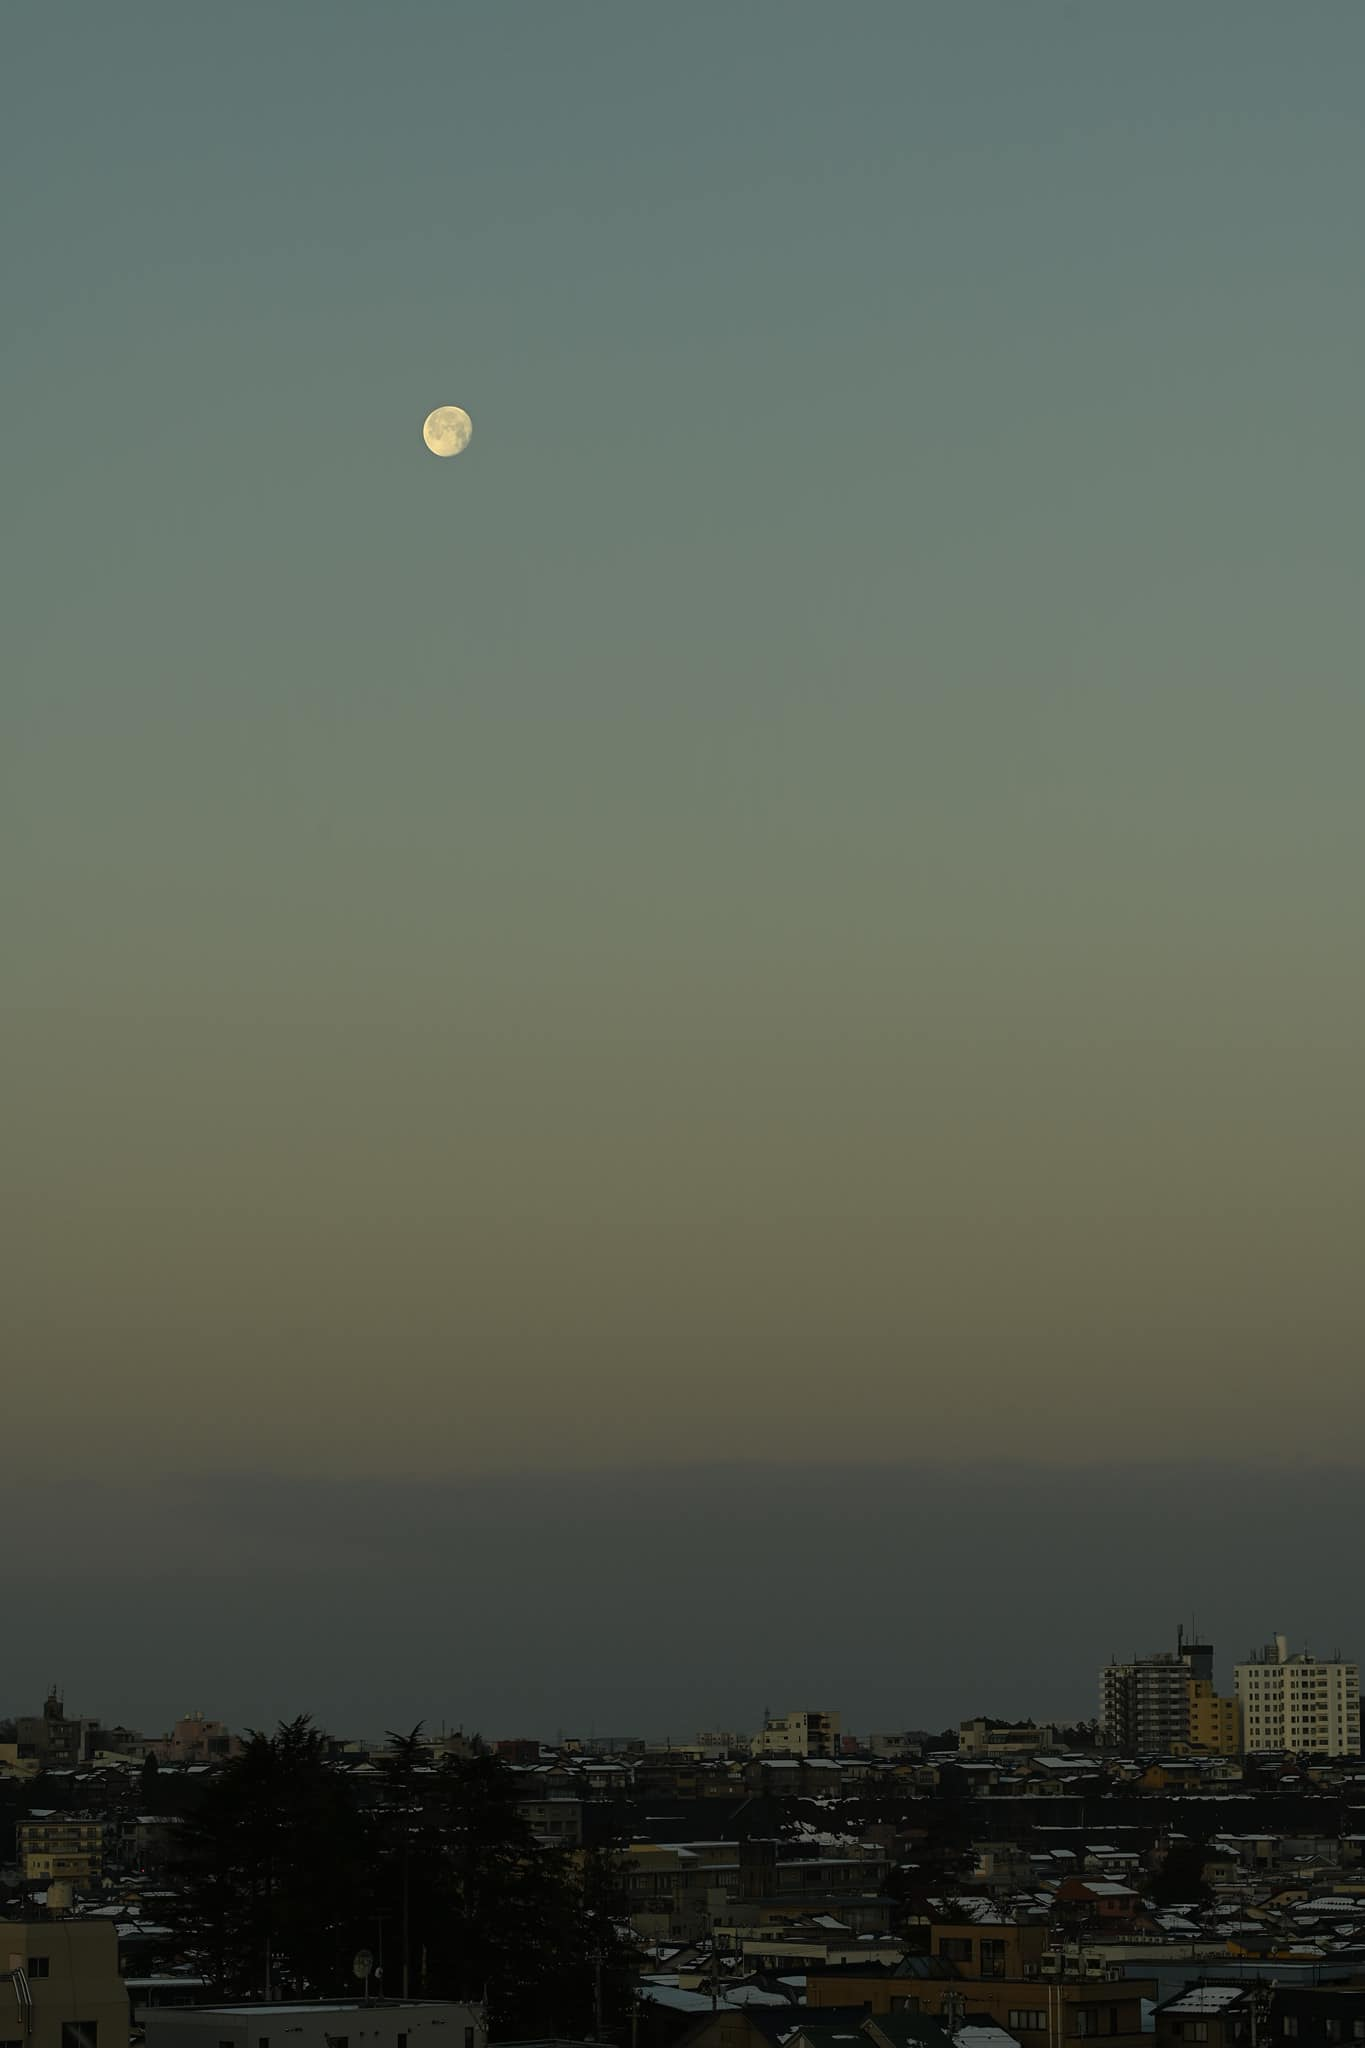
\includegraphics[width=\linewidth]{pictures/2025/02/20250215_085030_001.jpg}
\end{minipage}
\end{center}

\subsection*{2025年02月18日 09:48}
\addcontentsline{toc}{subsection}{2025年02月18日 09:48}

添付の番組をTVerで見ました。（2月20日までTVerで見られるらしい）


いまからサイエンス

\url{https://tver.jp/episodes/epxc8vr54c}



または、

\url{https://video.tv-tokyo.co.jp/imakara_science/episode/00119956.html}




この番組を信じるとすると、「誤差逆伝播法」のルーツは1967年の研究であり、「連想記憶」のホップフィールドネットワークのルーツは1972年の研究であり、「学習」のボルツマンマシンのルーツは1968年の研究にある。いずれのルーツも甘利先生の研究だとの事ですから、先駆者なんですね。甘利先生が受賞対象になっていたら、ヒントンもホップフィールドも受賞する理由がなくなってしまう様に思います。ヒントンとホップフィールドが受賞するには他の理由があったという事でしょうか。


ノーベル賞って昔は工業系の研究業績は対象になっていなかった様に思いますが、いつの間にか「実利への貢献」を顕彰する形に変わってきた様な気がします。その結果、理論的な面での先駆者ではあったけれども、実利への貢献が見られなかったという点で、外れてしまう事態になったのかもしれません。


\#甘利俊一 \#ノーベル賞 \#AI \#ホップフィールド \#ヒントン \#TVer \#QA4U3

\paragraph{写真}
\begin{center}
\begin{minipage}{0.48\linewidth}
\centering
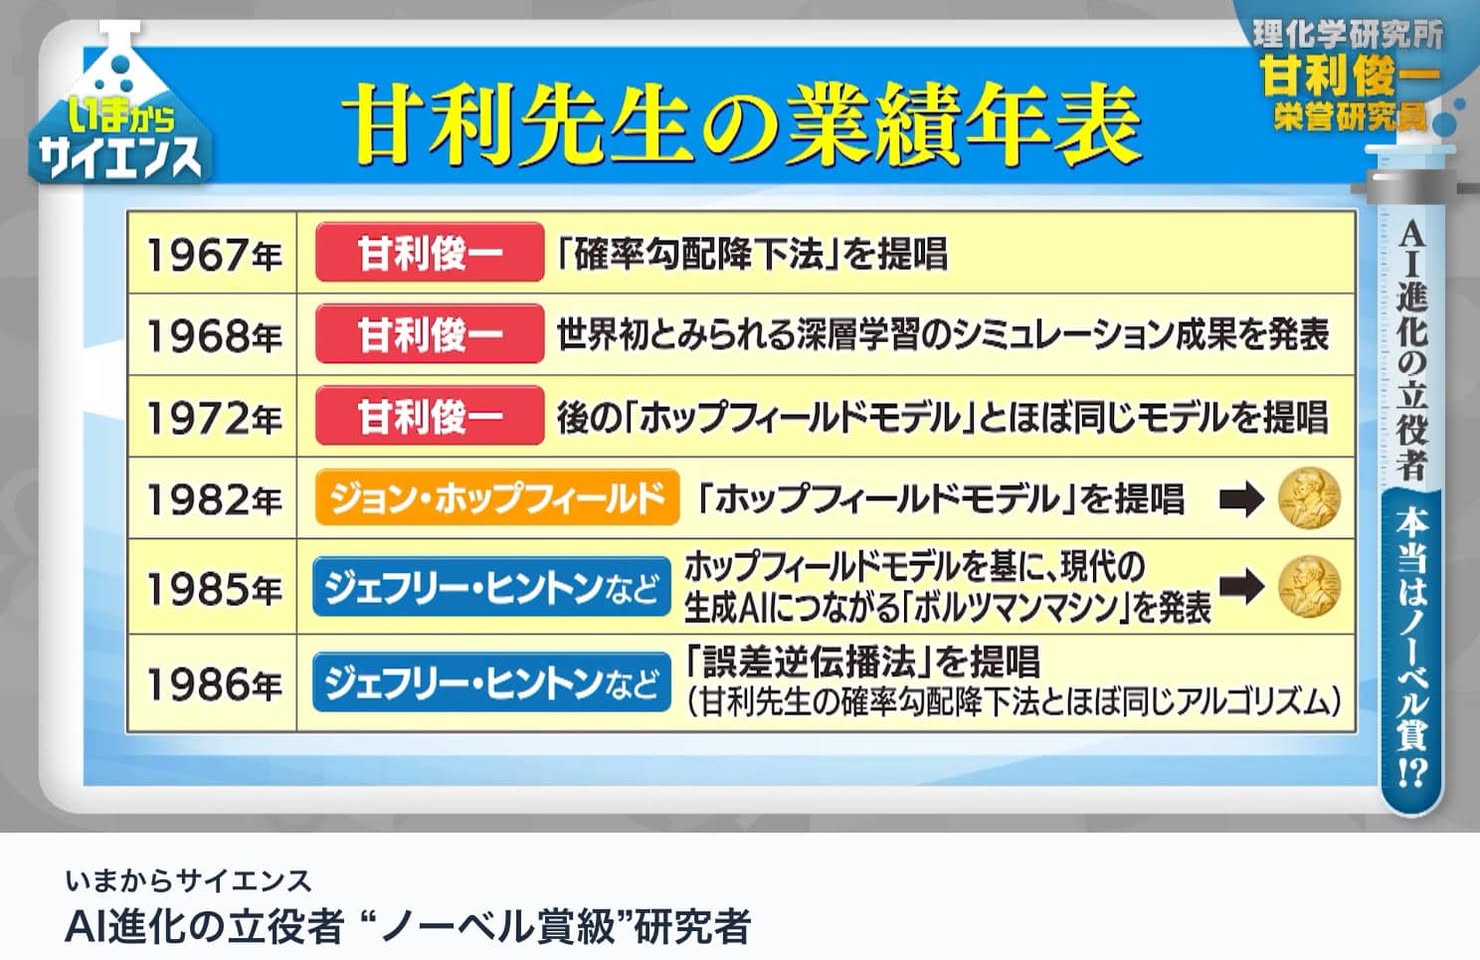
\includegraphics[width=\linewidth]{pictures/2025/02/20250218_094841_001.jpg}
\end{minipage}
\end{center}

\subsection*{2025年02月19日 06:24}
\addcontentsline{toc}{subsection}{2025年02月19日 06:24}

\paragraph{リンク}
\url{https://youtu.be/ErVUh3Pffyk}

\begin{center}
\href{https://youtu.be/ErVUh3Pffyk}{
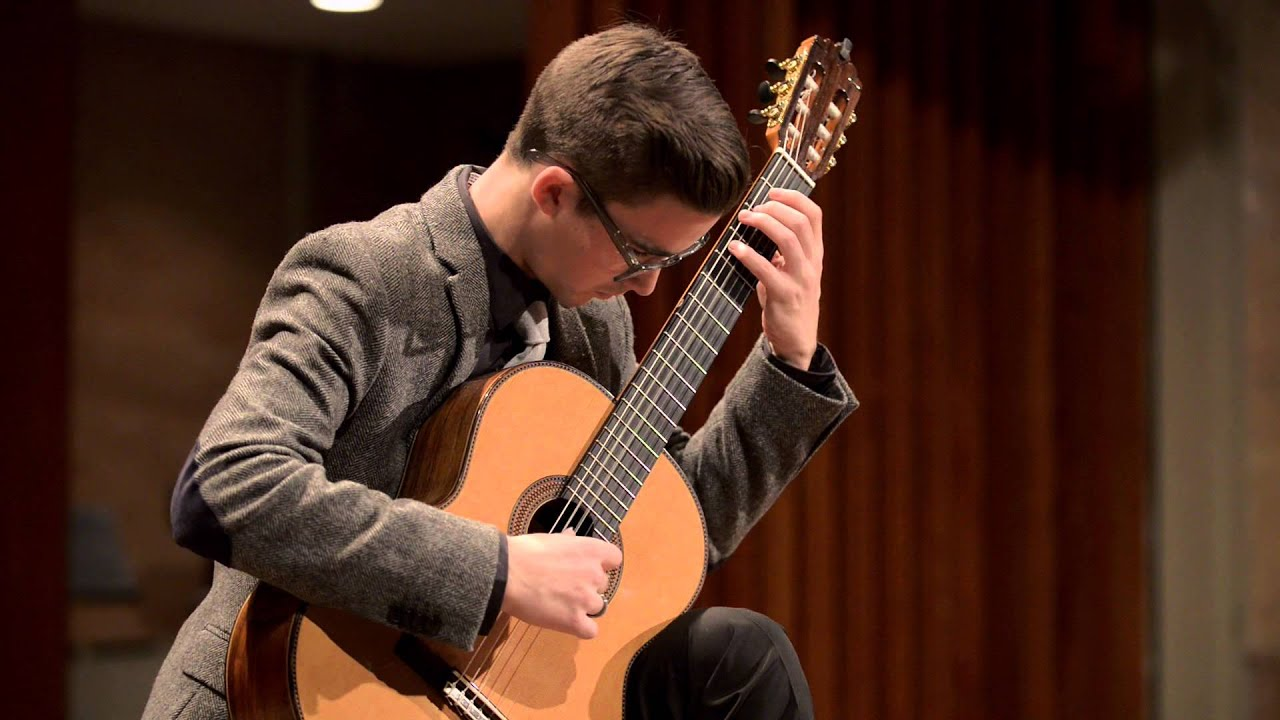
\includegraphics[width=0.48\linewidth]{pictures/youtube/2025/02/20250219_062453_youtube_001_ErVUh3Pffyk.jpg}
}
\end{center}

\subsection*{2025年02月19日 11:48}
\addcontentsline{toc}{subsection}{2025年02月19日 11:48}

\paragraph{リンク}
\url{https://youtu.be/eJzWs-LRdrc}

\begin{center}
\href{https://youtu.be/eJzWs-LRdrc}{
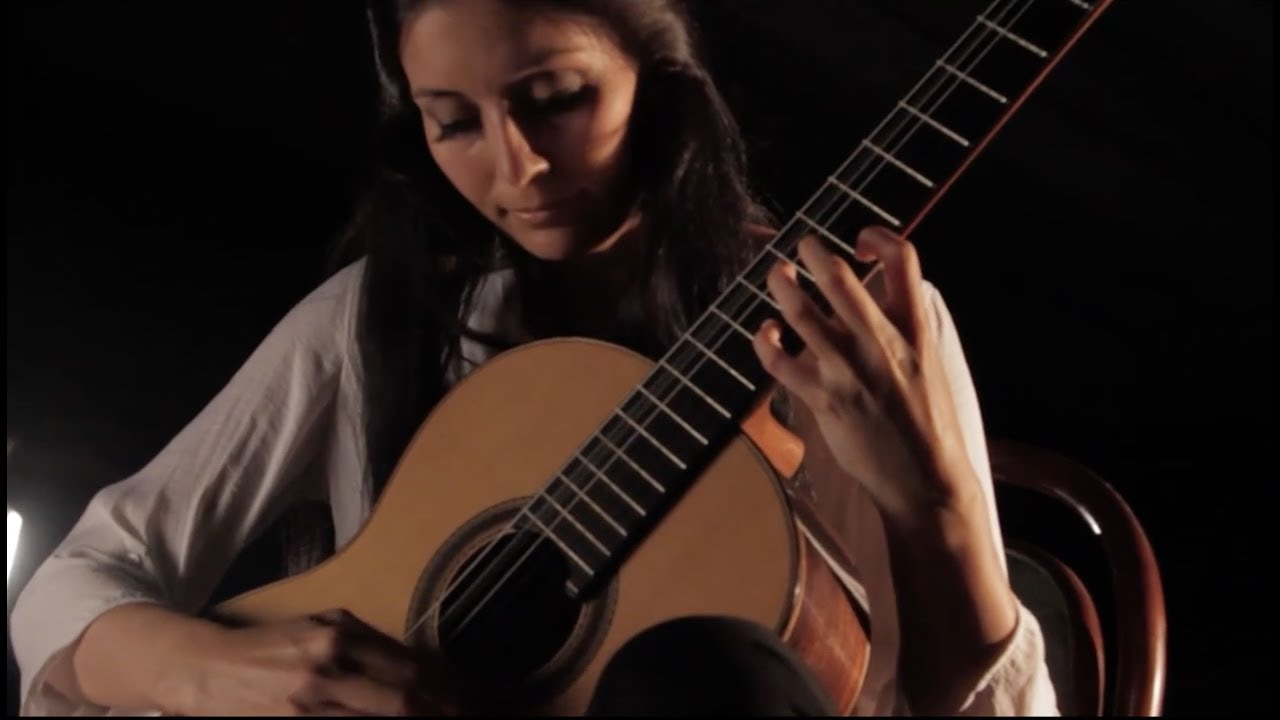
\includegraphics[width=0.48\linewidth]{pictures/youtube/2025/02/20250219_114818_youtube_001_eJzWs-LRdrc.jpg}
}
\end{center}

\subsection*{2025年02月21日 16:11}
\addcontentsline{toc}{subsection}{2025年02月21日 16:11}

\#量子コンピュータ のプログラムを試せるという \#QA4U3 プロジェクト（

\url{https://altema.is.tohoku.ac.jp/QA4U3/}

）で、第四回（

\url{https://youtu.be/MRX13sRRGsE}

\begin{center}
\href{https://youtu.be/MRX13sRRGsE}{
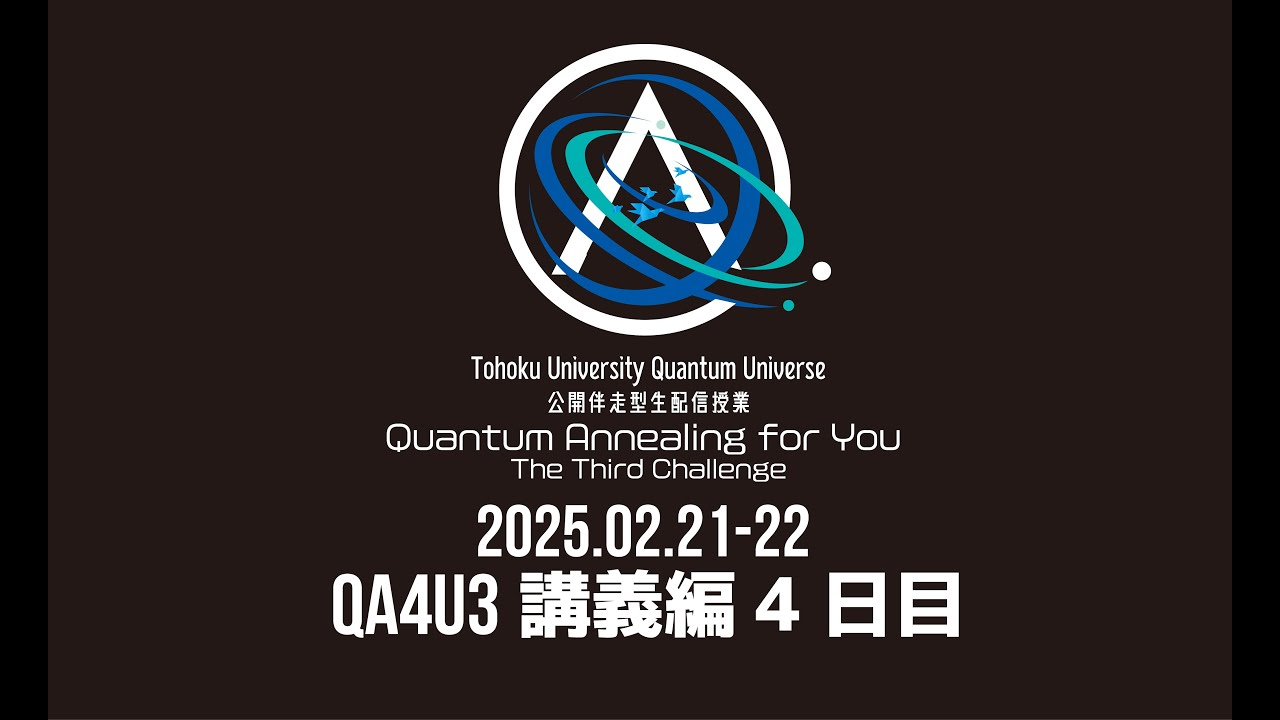
\includegraphics[width=0.48\linewidth]{pictures/youtube/2025/02/20250221_161151_youtube_001_MRX13sRRGsE.jpg}
}
\end{center}

）の講義を受講する予定です。（2月21日17時スタート）


（その後）第四回を一通り受講しました。

充実した内容でした。

(１) 数分割問題（Number Partition Completeness）

色んな重さの荷物がいくつもあって、それらをAさんとBさんで分担して運ぼうという時、Aさんがどれとどれとどれを持って、Bさんが残りを持つ事にしたら、2人の重さの負担をほぼ同じになる様にできますか？という話。

Aさんが持つ荷物の重さの合計からBさんが持つ重さの合計を引いて、その全体を自乗（Aさんの荷物の合計がBさんの荷物の合計より大きい組み合わせの場合もあれば、その逆の時もあるからね）した量を最小化Minimize（ゼロになれば其々の重さの合計は全く等しいのだけど、普通は全く一緒にならないから、最小化を目指す事に）する様な荷物の組み合わせを、量子コンピュータ君に見つけさせる。


(２) 複数のグループに分ける

20人を5つのグループに分ける時、仲良しもいれば、絶対一緒のグループは嫌という人もいる。誰と誰と誰と誰でAグループにするみたいに、どんなグループ分けをしたら、全体として良好な（最大のパフォーマンスを出せる）グループ分けになるか？という問題。

2人（i1君とi2君）毎の相性を表す行列Ci1i2を決めて、j番目のグループに属する、0或いは1を取り得る変数xji1とxji2を掛けて足した量を最大化Maximizeする様なグルーピングを、量子コンピュータ君に決めてもらう。1人は複数のグループに属さないこととするとか、1グループは４人にするなどの制約条件を与えて計算させる事ができる。


(３) 非負値行列分解（NMF：Non Negative Matrix Factorization）

顔の画像データ（沢山ある）セットから1枚取り出しては、その画像がどんな画像の重ね合わせからできているのかを見つけ出させる事を、全部の画像データに対して行い、それぞれの時のQUBO行列に対して、ボルツマンマシンの時の様に更新を繰り返していく事によって、顔画像データセットが持っている顔情報を構成する、基となる画像の一式が求まる。逆にその基画像を足し合わせると、顔画像データセットにある人の様な顔画像を合成できる。

トランプさんの色んな画像を学習させたら、トランプさんぽい顔を合成するための基本画像データの一式を用意できるという事かな？

（面白そうだけど、フェイクニュース等に悪用してはいけません）

\subsection*{2025年02月23日 00:10}
\addcontentsline{toc}{subsection}{2025年02月23日 00:10}

\paragraph{リンク}
\url{https://youtu.be/MRX13sRRGsE}

\begin{center}
\href{https://youtu.be/MRX13sRRGsE}{
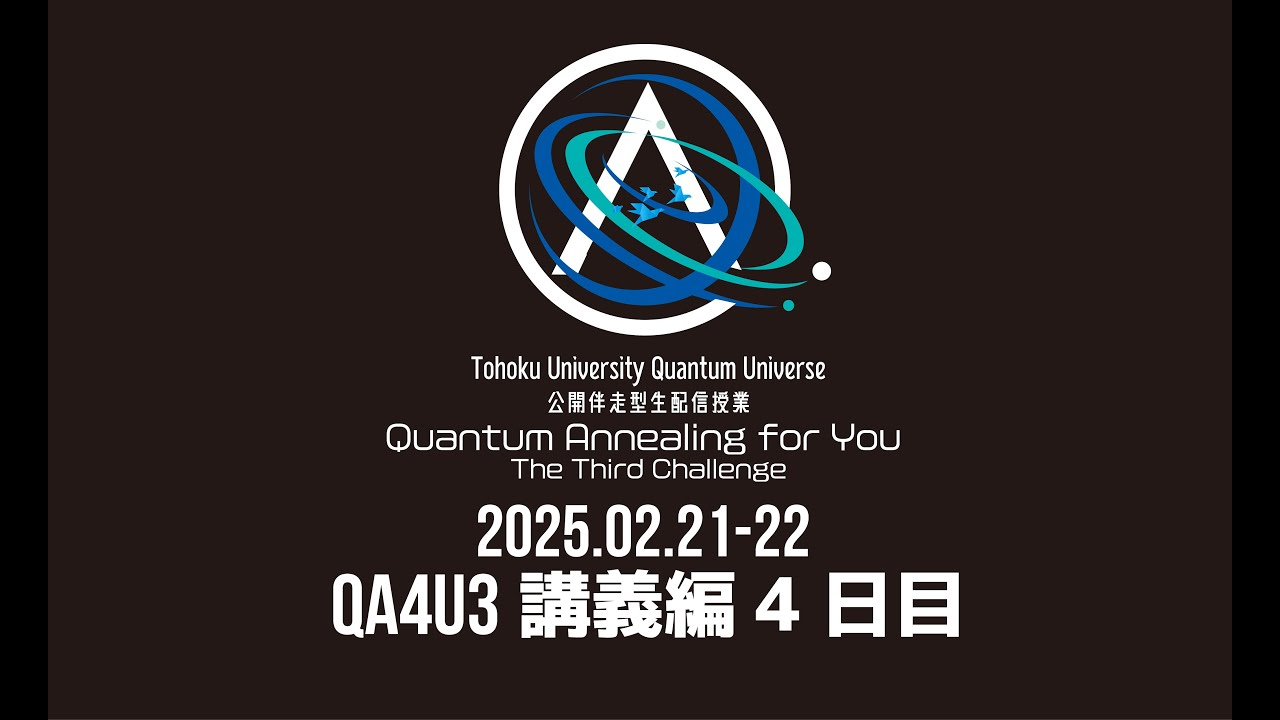
\includegraphics[width=0.48\linewidth]{pictures/youtube/2025/02/20250223_001041_youtube_001_MRX13sRRGsE.jpg}
}
\end{center}

\subsection*{2025年02月24日 17:53}
\addcontentsline{toc}{subsection}{2025年02月24日 17:53}

\paragraph{リンク}
\url{https://x.com/manabu16/status/1893172151697711257}

\subsection*{2025年02月27日 08:15}
\addcontentsline{toc}{subsection}{2025年02月27日 08:15}

\url{https://typst.app/}




最近巷では、TeXではなく、このTypstなるものが流行っているらしい。しばらく使ってみようかな。

\subsection*{2025年02月27日 08:18}
\addcontentsline{toc}{subsection}{2025年02月27日 08:18}

\paragraph{リンク}
\url{https://typst.app/}

\section{3月}

\subsection*{2025年03月06日 08:08}
\addcontentsline{toc}{subsection}{2025年03月06日 08:08}

\#量子コンピュータ のプログラムを試せるという \#QA4U3 プロジェクト（

\url{https://altema.is.tohoku.ac.jp/QA4U3/}

）で、第五回（

\url{https://youtu.be/g3RZkwEI300}

\begin{center}
\href{https://youtu.be/g3RZkwEI300}{

\includegraphics[width=0.48\linewidth]{pictures/youtube/2025/03/20250306_080848_youtube_001_g3RZkwEI300.jpg}
}
\end{center}

）の講義を受講しました。（2月28日17時スタート）


このプロジェクトQA4U3では、この後グループに分かれて、実際に量子コンピュータを使って、社会に内在する様々な課題の解決や応用アプリの開発などを、グループ毎に進めていくという事らしいのですが、そのグループ分けを量子コンピュータにやらせるという事で、その手順を、順にプログラムを作りながら解説されていた。


とても参考になった事があった。これまでは、変数を登録したり、問題を定義したり、制約条件を加えたりしていくと、自動的にqubo行列が出来上がって、それをsamplerに渡して解いていたのだが、最初からそのツールに頼らずに自前のQUBO行列を作るプログラムのやり方が解説されていた。これは使えるという気がしましたよ。


samplerに渡すまで特別のツールに頼らず自分でプログラムするという事ですから、余計なものをpip install 何某としなくてもよいというわけです。samplerさえinstallしておけば、後は自分でモデルをゼロからプログラムして、量子コンピュータのシミュレータに渡せるのですから。（実はこのシミュレータも、何とか自前にならないものかとさえ思ってしまいます）


パソコンでの処理は主にCPUがやる訳ですが、グラフィック画面の処理（や行列の計算）をGPUが分担し、量子計算を（シミュレータではなくて実際の）QPUが分担するという形の、次世代型ノートパソコンがあるとよいのだが、という気になります。でも、私の目ん玉が黒いうちにQPUがノートに載る様なチップになる可能性は低いでしょうね。量子コンピュータの現状はと言えば、理化学研究所の天井にぶら下がる大きなシャンデリアみたいな（しかも超伝導になるまで冷却されている）状態なのですから。

\subsection*{2025年03月06日 08:27}
\addcontentsline{toc}{subsection}{2025年03月06日 08:27}

\paragraph{リンク}
\url{https://youtu.be/g3RZkwEI300}

\begin{center}
\href{https://youtu.be/g3RZkwEI300}{

\includegraphics[width=0.48\linewidth]{pictures/youtube/2025/03/20250306_082758_youtube_001_g3RZkwEI300.jpg}
}
\end{center}

\subsection*{2025年03月06日 14:19}
\addcontentsline{toc}{subsection}{2025年03月06日 14:19}

石川県 \#金沢 市 \#犀川 縁にある「\#穂濤（杉の井）」で食事をしました。（\#ミシュラン 二つ星）

\url{http://kanazawa-suginoi.co.jp}




落ち着いた部屋と上品な食事を堪能できました。

（予約をとろうとしても、一回目はダメでしたよ）


部屋には、\#室生犀星 の「犀川」の書が掛けられていました。


\#抒情小曲集 犀川


うつくしき川は流れたり

そのほとりに我は住みぬ

春は春、なつはなつの

花つける堤に座りて

こまやけき本のなさけと愛とを知りぬ

いまもその川ながれ

美しき微風ととも

蒼き波たたへたり


（青空文庫 

\url{https://www.aozora.gr.jp/cards/001579/files/53241_49665.html}

）


こんなに美しい詩でふるさとを謳いながら、

一方では、ふるさとは決して帰る所じゃない、

などと言わせる気持ちとは、どの様なものだったのか。


（添付の写真）

右手、タクシーの停まっているところが出入り口。

左手、犀川と奥に見えるのは \#桜橋。（この橋の橋詰には右に \#新桜坂、左に \#桜坂、真ん中には \#W坂 があって、\#寺町 に登る主要道路になっている）

写真の真ん中の桜の樹の幹は堤と一体になった様に育っている。この幹の様子を見ると、（コンクリート製とは言え）この堤自体の歴史も長そうです。

室生犀星氏の幼い頃に、この堤の辺りに座って本を読まれていた事があったかもしれません。

\paragraph{写真}
\begin{center}
\begin{minipage}{0.48\linewidth}
\centering
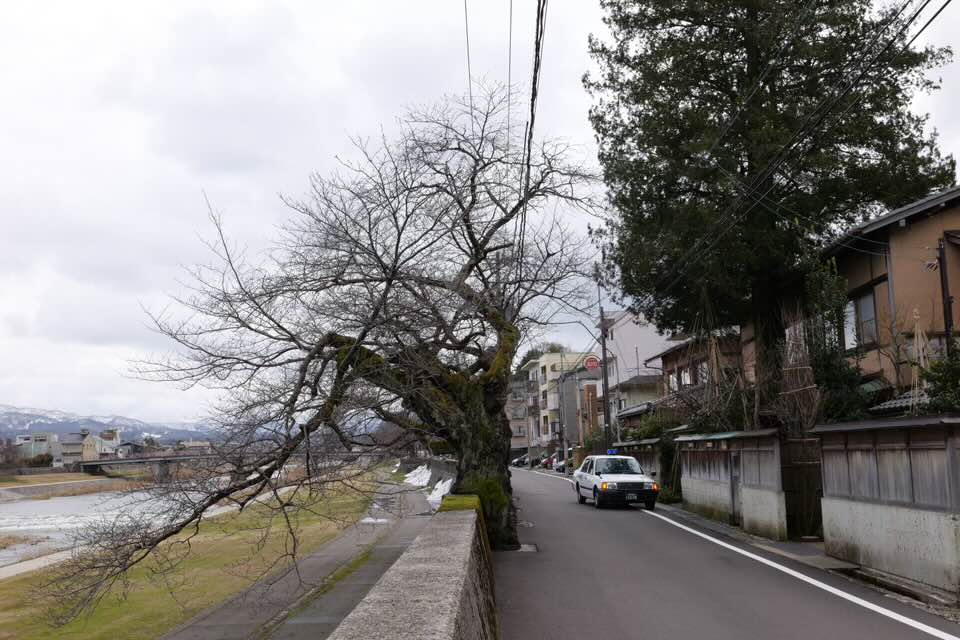
\includegraphics[width=\linewidth]{pictures/2025/03/20250306_141941_001.jpg}
\end{minipage}
\end{center}

\subsection*{2025年03月07日 12:54}
\addcontentsline{toc}{subsection}{2025年03月07日 12:54}

\paragraph{リンク}
\url{https://youtu.be/c3NLIR4T9vk}

\begin{center}
\href{https://youtu.be/c3NLIR4T9vk}{
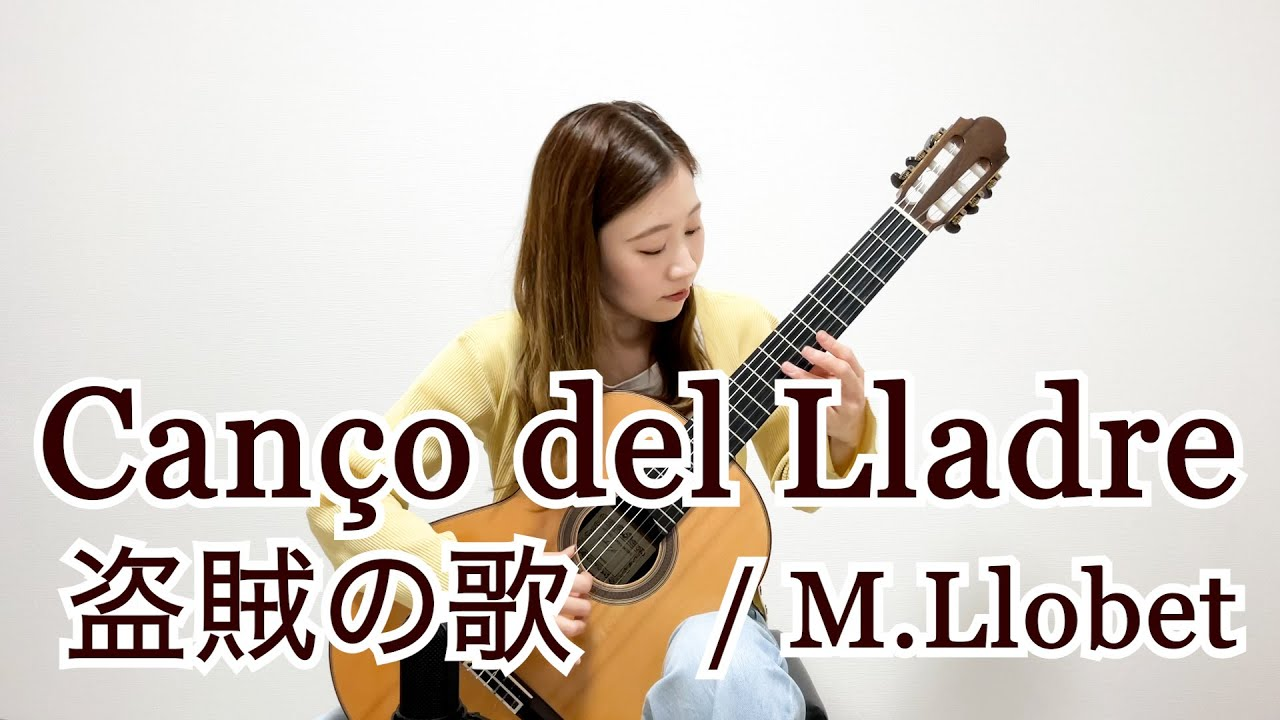
\includegraphics[width=0.48\linewidth]{pictures/youtube/2025/03/20250307_125445_youtube_001_c3NLIR4T9vk.jpg}
}
\end{center}

\subsection*{2025年03月07日 23:49}
\addcontentsline{toc}{subsection}{2025年03月07日 23:49}

\#量子コンピュータ のプログラムを試せるという \#QA4U3 プロジェクト（

\url{https://altema.is.tohoku.ac.jp/QA4U3/}

）で、第六回（

\url{https://youtu.be/_tL5P3sS5uk}

\begin{center}
\href{https://youtu.be/_tL5P3sS5uk}{

\includegraphics[width=0.48\linewidth]{pictures/youtube/2025/03/20250307_234942_youtube_001__tL5P3sS5uk.jpg}
}
\end{center}

）の講義を受講しました。（3月7日17時スタート）


この後はグループ活動に入るようです。

\subsection*{2025年03月22日 17:25}
\addcontentsline{toc}{subsection}{2025年03月22日 17:25}

\paragraph{リンク}
\url{https://youtu.be/M_iBbTofuFQ}

\begin{center}
\href{https://youtu.be/M_iBbTofuFQ}{
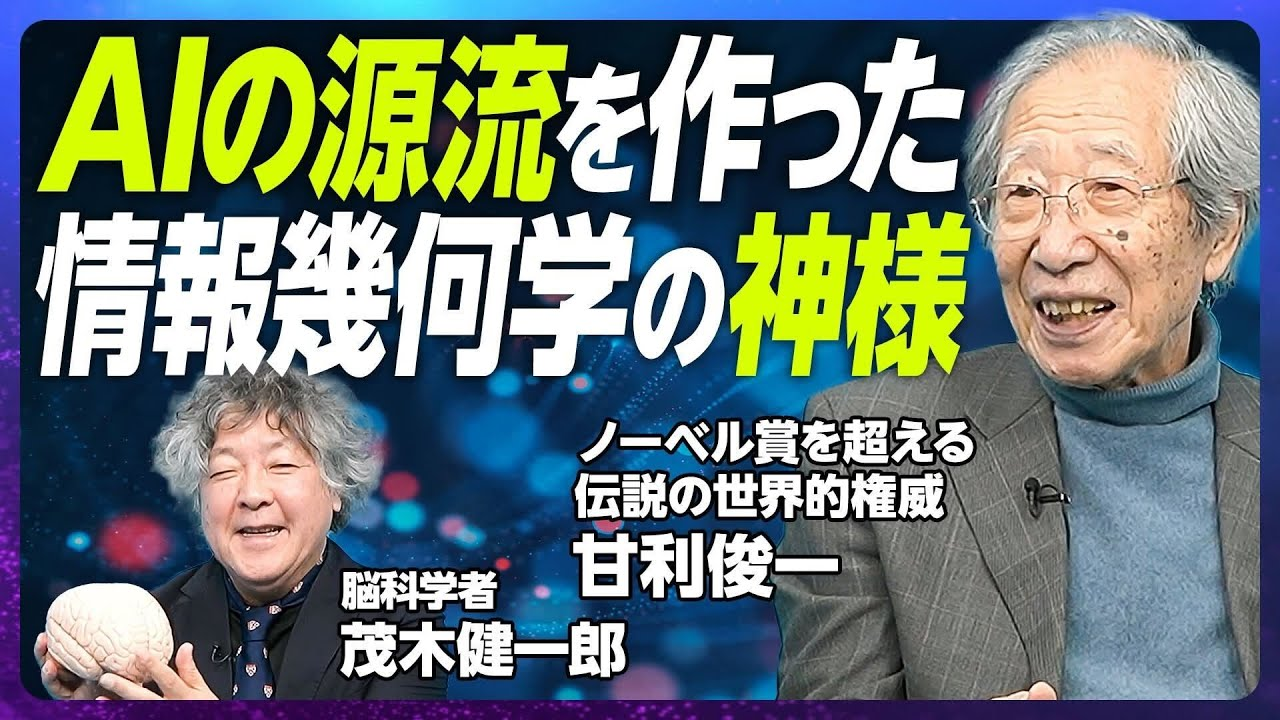
\includegraphics[width=0.48\linewidth]{pictures/youtube/2025/03/20250322_172515_youtube_001_M_iBbTofuFQ.jpg}
}
\end{center}

\subsection*{2025年03月24日 13:23}
\addcontentsline{toc}{subsection}{2025年03月24日 13:23}

\url{https://youtu.be/9yo3D4muNsw}

\begin{center}
\href{https://youtu.be/9yo3D4muNsw}{
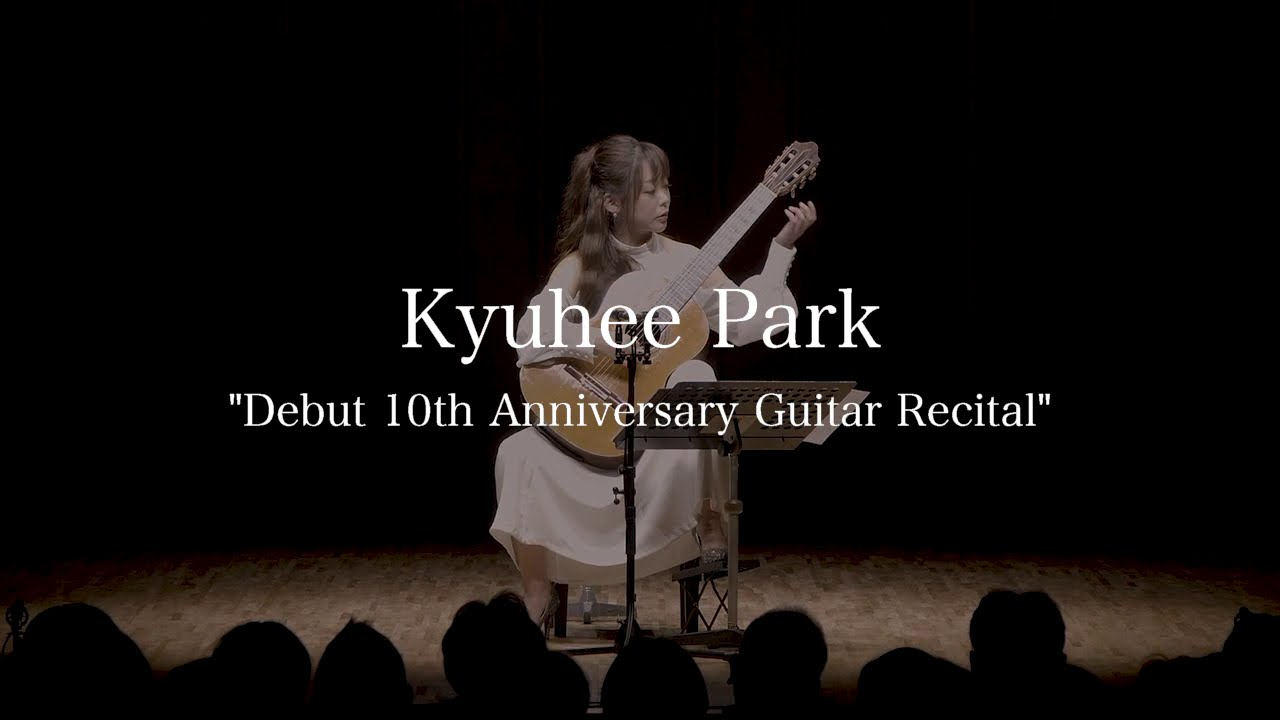
\includegraphics[width=0.48\linewidth]{pictures/youtube/2025/03/20250324_132349_youtube_001_9yo3D4muNsw.jpg}
}
\end{center}




パク・キュヒ氏によるアダージェットの演奏はYouTube上に複数見られますが、この時の演奏が良いような気がします。（編曲は佐藤弘和氏）

マーラーを一本のギターで演奏するなどと、、凄いなあ。（挑戦しようとはとても思わないけれども）

\subsection*{2025年03月24日 22:41}
\addcontentsline{toc}{subsection}{2025年03月24日 22:41}

\paragraph{リンク}
\url{https://youtu.be/y_nTZtvP0aI}

\begin{center}
\href{https://youtu.be/y_nTZtvP0aI}{
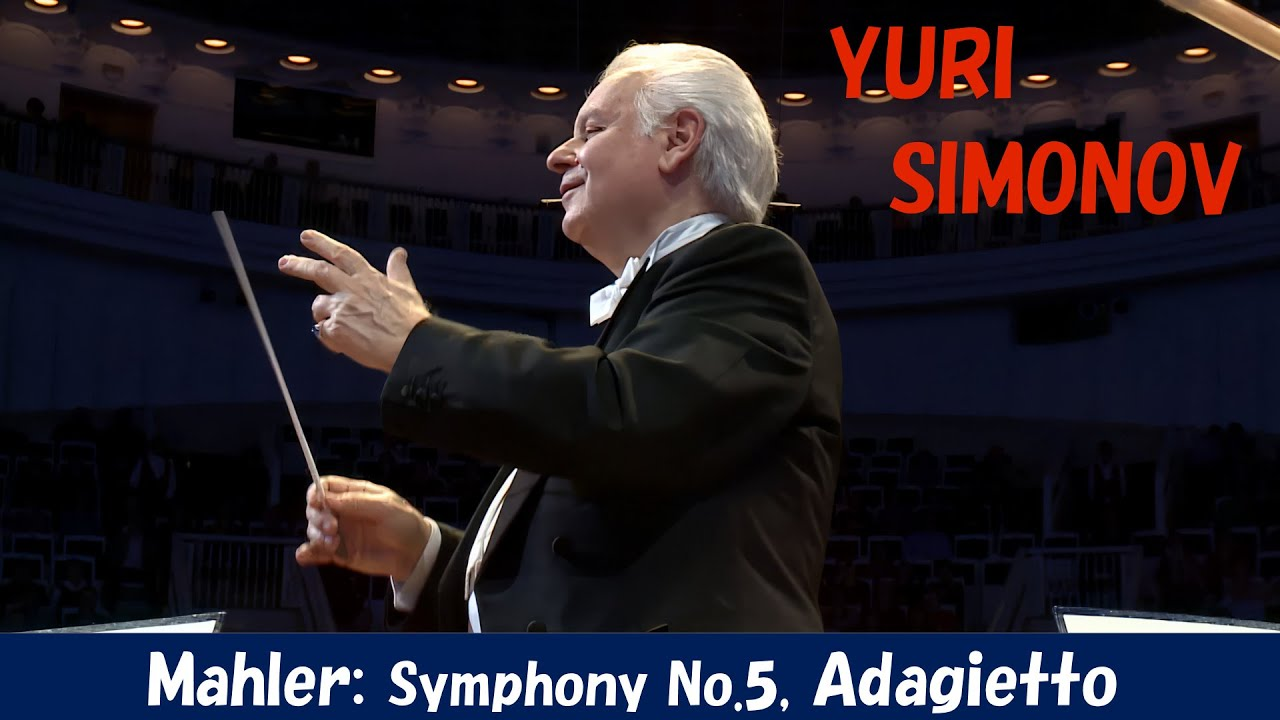
\includegraphics[width=0.48\linewidth]{pictures/youtube/2025/03/20250324_224113_youtube_001_y_nTZtvP0aI.jpg}
}
\end{center}

\subsection*{2025年03月24日 22:46}
\addcontentsline{toc}{subsection}{2025年03月24日 22:46}

\paragraph{リンク}
\url{https://youtu.be/0KHVtDgfVZg}

\begin{center}
\href{https://youtu.be/0KHVtDgfVZg}{

\includegraphics[width=0.48\linewidth]{pictures/youtube/2025/03/20250324_224656_youtube_001_0KHVtDgfVZg.jpg}
}
\end{center}

\subsection*{2025年03月25日 03:46}
\addcontentsline{toc}{subsection}{2025年03月25日 03:46}

\paragraph{リンク}
\url{https://www.nhk.jp/g/pr/blog/diu62i_irv/}

\subsection*{2025年03月27日 09:40}
\addcontentsline{toc}{subsection}{2025年03月27日 09:40}

\#文部科学省 のサイト（

\url{https://www.mext.go.jp/a_menu/koutou/ichiran/mext_00026.html}

）で公開されている \#大学情報 の \#Excel ファイルから、[国公私立の区別]、[大学名]、[学部名]、[学科名]、[都道府県名]、[市町村名]、の格好の \#CSV （ \#JSON ）を出力するためのプログラムを（とある必要があって）作ってみた。

最初CSVのつもりでファイル名を ”.csv” などとしていたけど、最終的にJSONで書き出す事にした。（最近はCSVに代えてJSONでというのが流れだろうと思う）ファイル名や関数名等、本来なら改めた方が良いですね。


大学名はシート名からとってきている。

“学部”という文字が１列目に現れたら、その時の行番号の「次の次の次の行」から学部学科等の情報が記述されている。学部や学科の名前が3列目、5列目に、都道府県名と市町村名が６列目と８列目に書かれているので、それらを書き出していく。

学部学科等の情報の終わりは、（取り敢えず）1列目と3列目を見ていて、どちらも空なら終わりだと判断している。


これを国立大学のExcelファイルの初めの方のシートで試行錯誤して、何となく目星をつけ、やってみたら、公立のファイルも、私立の８つのファイルも同様になっている様で、問題なくCSV（JSON）出力できました。


\#GitHub に置いておこうと思います。

\url{https://github.com/smat1957/QA4U/tree/main/excel2csv}



\paragraph{写真}
\begin{center}
\begin{minipage}{0.48\linewidth}
\centering
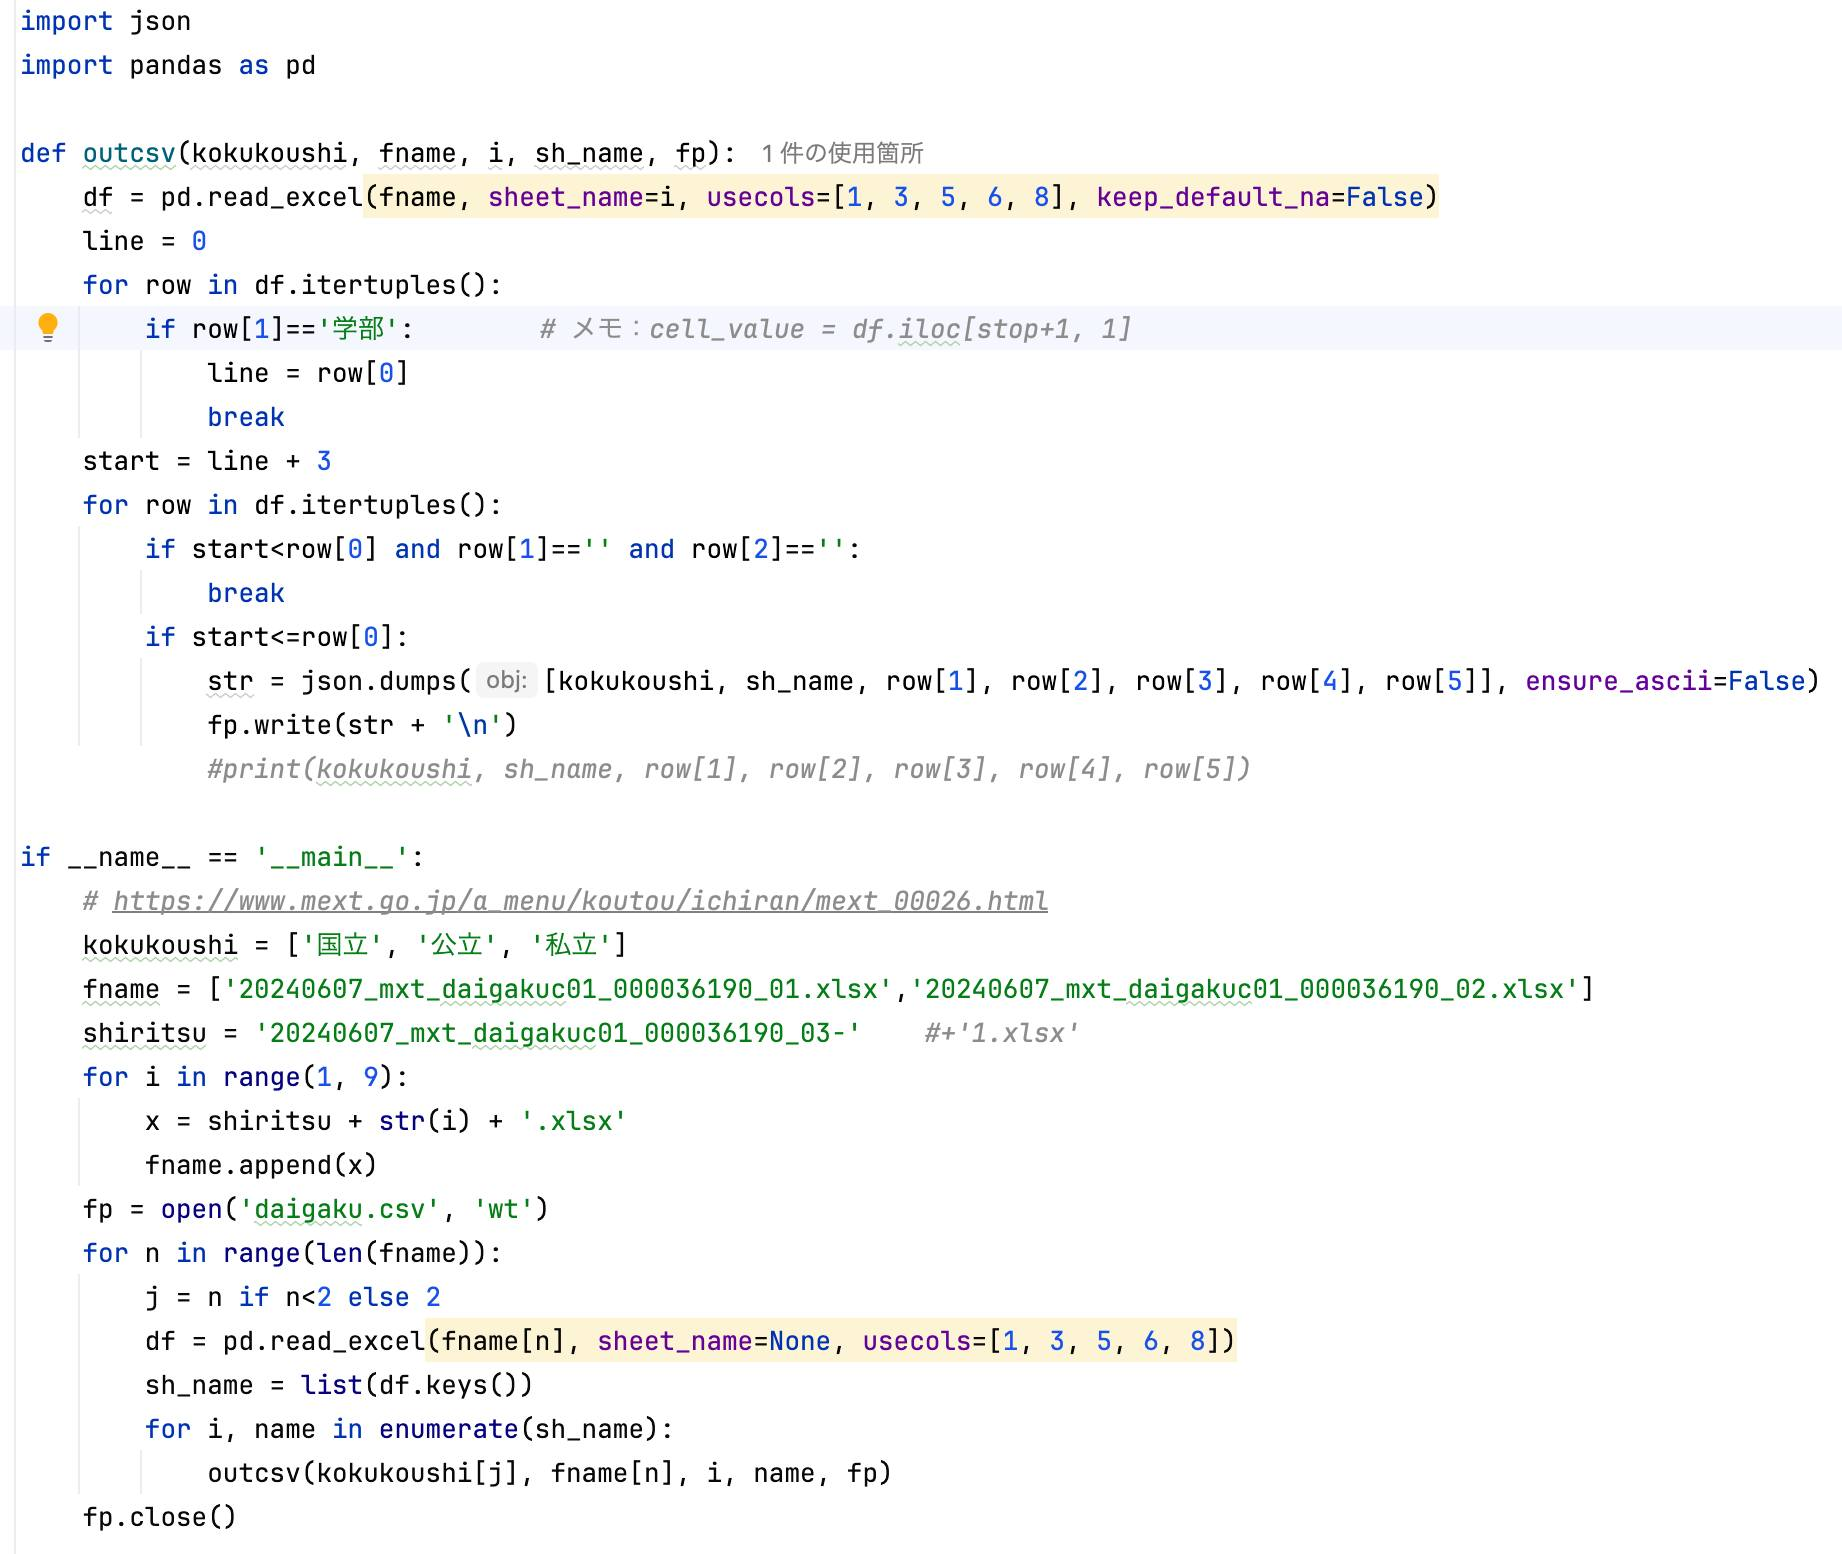
\includegraphics[width=\linewidth]{pictures/2025/03/20250327_094036_001.jpg}
\end{minipage}
\end{center}

\subsection*{2025年03月27日 17:13}
\addcontentsline{toc}{subsection}{2025年03月27日 17:13}

\#swift から（或いはJavaでもそうなのだが）\#python のプログラムを呼び出さなければならないケースは、とてもニーズが高いものと推察します。それは、swiftがMacやiPhone上でのUIの構成に優れているのに対して、pythonはswift（やJava）には無い有用なライブラリ（AI や統計関連）が多数あるからです。そこで、swiftからpythonを呼び出す処理を、実際に試してみる事にしました。もちろんネットを調べればある程度は出てくるのですが、多くの場合「帯に短し襷に長し」の状態なので、まるまるコピペで済むというわけにはいきません。


「 \#仮想環境 の中で実行させるpythonと、swiftとの間で情報のやり取りを行う場合」について試行しました。


「ああでもないこうでもない」と試行錯誤した結果、添付の通りとなりました。やっている事は次の通りです。（\#Mac の \#デスクトップ 環境で試しています）


(１) 仮想環境に入って、pythonを起動し、処理の終了後に仮想環境から抜けるという一連の処理を \#シェル に書いておきます

(２) そのシェルをswiftから \#サブプロセス で起動します

(３) swiftから渡す情報は、シェルの順序引数で受け取らせ、それをpythonの \#コマンドライン引数 として渡しています

(４) pythonがprint文などで吐き出す \#標準出力 は、\#パイプ でswiftに \#リダイレクト される様にしています


swiftの中で、

print( python01 ( cmdlineargs: [“1”, “2”, “3”] ) )

として呼び出してやれば、

“1 + 2 + 3 = 6”

という文字列が返ってくると思います。

\paragraph{写真}
\begin{center}
\begin{minipage}{0.48\linewidth}
\centering
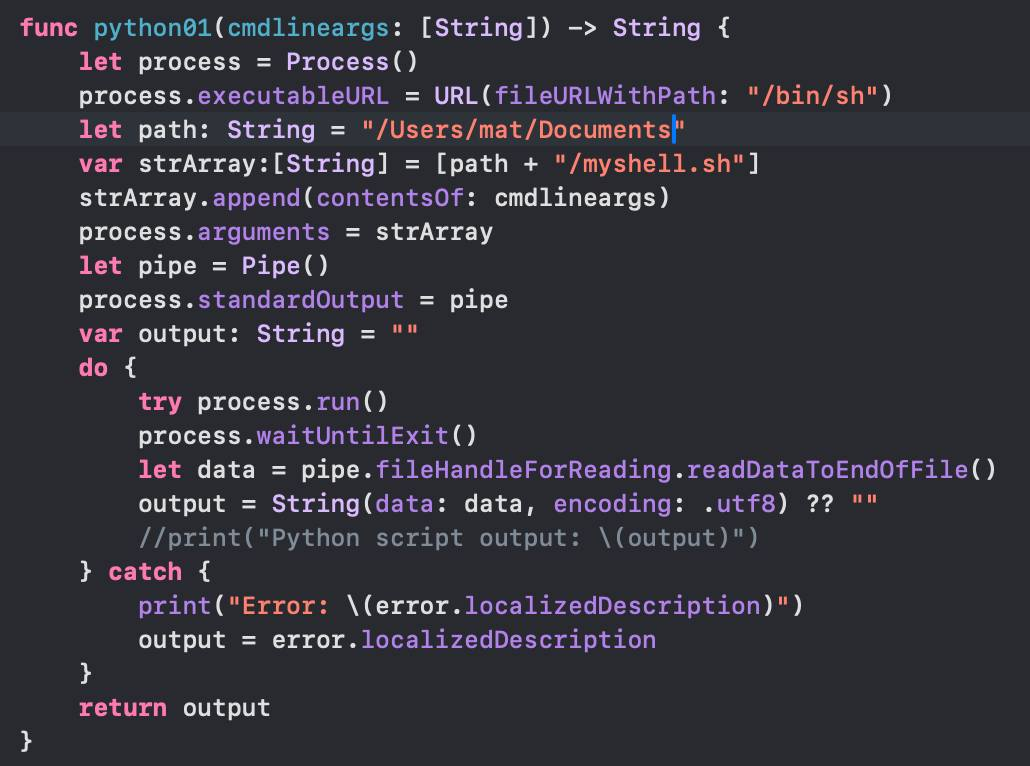
\includegraphics[width=\linewidth]{pictures/2025/03/20250327_171308_001.jpg}
\end{minipage}
\hfill
\begin{minipage}{0.48\linewidth}
\centering
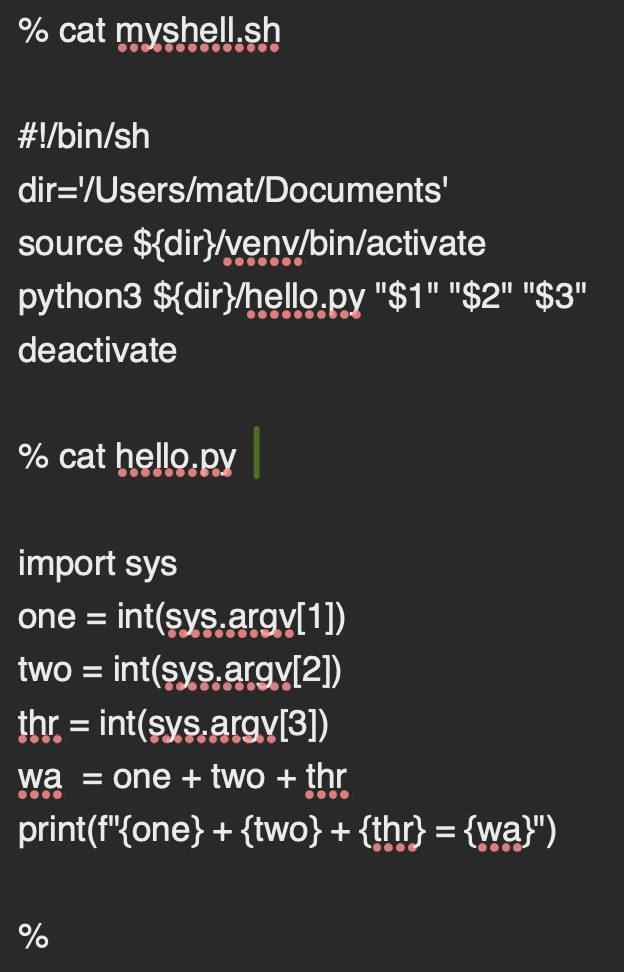
\includegraphics[width=\linewidth]{pictures/2025/03/20250327_171308_002.jpg}
\end{minipage}
\end{center}

\subsection*{2025年03月27日 21:16}
\addcontentsline{toc}{subsection}{2025年03月27日 21:16}

\#Python の \#IDE の \#PyCharm を使って \#量子コンピュータ のためのプログラムを書いていた時の事です。


キー部が2要素の \#タプル で、値部分が実数である辞書型データ \#QUBO を作りたかったのですが、\#JSON ロードで得られるデータのキー部が、タプルの格好をした”文字列“だったため、JSONロード終了後の処理でプログラムは異常終了していました。


そこで、キー部を文字列からタプルに変換しようとして「すったもんだ」していたところ、何と！ \#AI assistant （

\url{https://www.jetbrains.com/ai/}

）などというものが、横から急に何か言い出してきて（「こんな事分かんないの？」と言わんばかりに）、添付のようなソースが自動的に生成され、私のプログラムの中に埋め込まれてきました。（勝手に！）

添付は生成されたソースの全てですが（コメントも日本語で付いています）ヒントなどではなく、そのまま使える関数としてできあがった形で生成されているのにビックリです。


私がプログラムでやろうと「すったもんだ」していた事というのは、生成されたプログラムの中では、with openの文でJSONデータをcmat にロードする2行と、その後、try文の下の2行をcmatの中の各項目に対して施す事、ただその部分だけなのですが、生成されたコードでは、色々な可能性を潰そうとしてきているのがわかります。


私が「すったもんだ」していた事を、AIが横から見ていて理解してくれていたという事でしょうか？すごい時代になったものだ。『注意深く利用すれば』プログラムの生産性は飛躍的に高まるでしょうね。


===

続き

\url{https://m.facebook.com/story.php?story_fbid=9384718338278910&id=100002225117991}



\paragraph{写真}
\begin{center}
\begin{minipage}{0.48\linewidth}
\centering
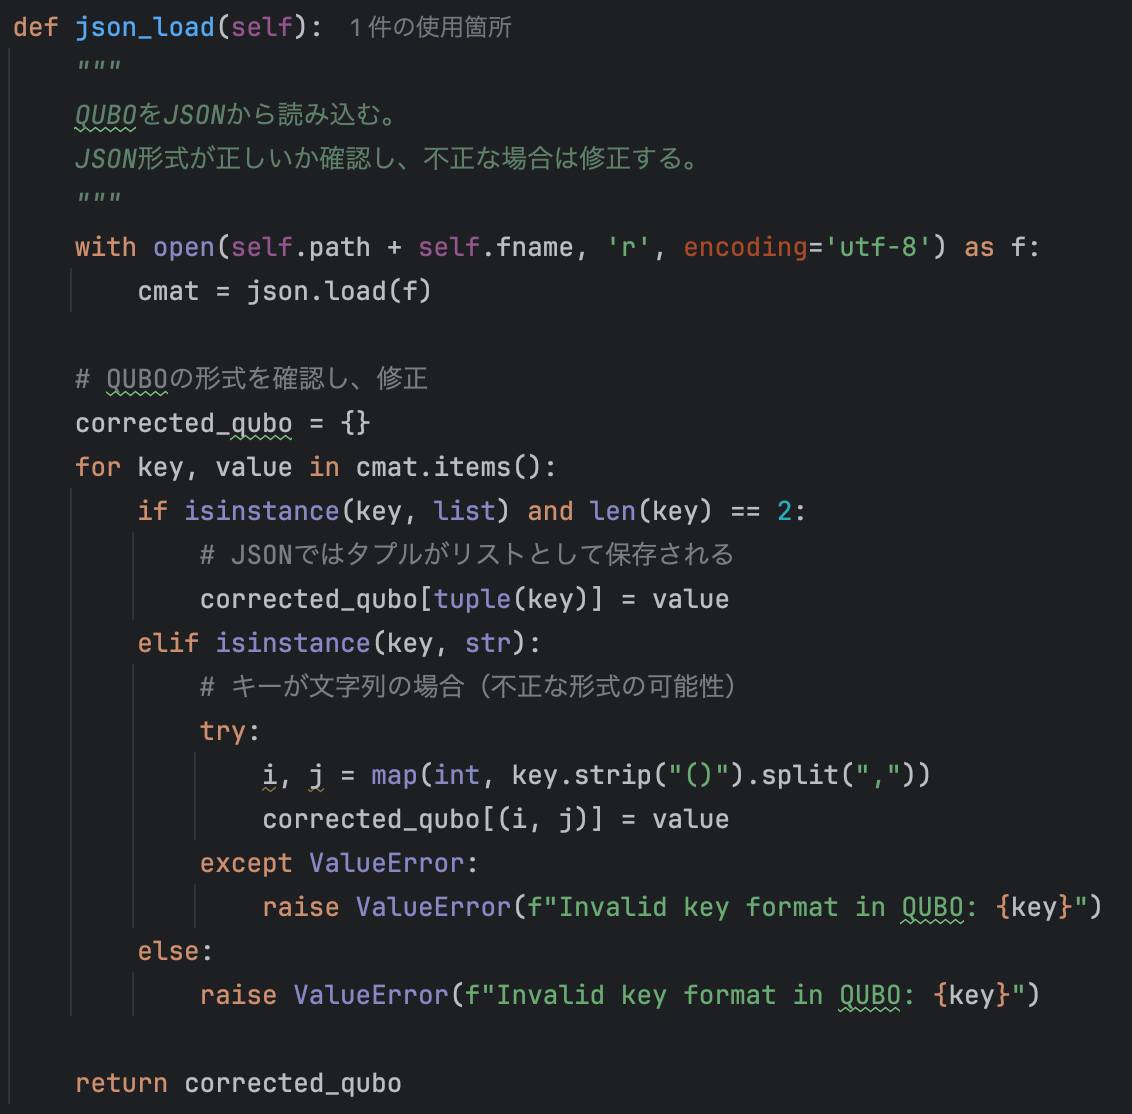
\includegraphics[width=\linewidth]{pictures/2025/03/20250327_211625_001.jpg}
\end{minipage}
\end{center}

\subsection*{2025年03月28日 16:07}
\addcontentsline{toc}{subsection}{2025年03月28日 16:07}

\#量子コンピュータ を使って \#グループ分け をするための \#QUBO を生成する関数を \#Swift で書いた。


G は1グループ当たりの人数、Mは全体の人数、MをGで割った整数値Kがグループの数です。zmatはM人それぞれの性格を持たせている行列です。M人それぞれにC個の特性をもたせているとすると、MxC行列ができるのだが、その転置行列C行M列を右からかけると、MxMの正方行列ができる。それがzmat。


(１)最初のfor k: for i: for j でQUBOは基本的に出来上がっている。coeff=1.0は \#最小化問題 （なるべく違う性質のもの同士のグループを作る）のとき、coeff=-1.0は \#最大化問題 （なるべく同じ性質のもの同士のグループを作る）の場合です。


(２) 次のfor i: for k1: for k2 では1人1グループ、同じ人が複数のグループに属さない様にする \#罰金法 です。lambda 1は制約の強弱を調整するパラメータです。


(３) 最後の for k: for i: for j では、１グループ当たりの人数をG人に揃える制約です。lambda 2は制約の強弱を調整するパラメータです。


QUBOは \#辞書型変数 で、キー部は２変数の \#タプル の格好をした文字列、値部分は実数値です。ここで作ったQUBO を \#JSON ダンプでファイルに出力して、PythonのプログラムでそのファイルをJSONロードさせます。そこで、キー部の文字列をタプルに変換したQUBOに作り直して（

\url{https://m.facebook.com/story.php?story_fbid=9385779461506131&id=100002225117991}

）

それを 量子コンピュータ に渡す事になります。

\paragraph{写真}
\begin{center}
\begin{minipage}{0.48\linewidth}
\centering
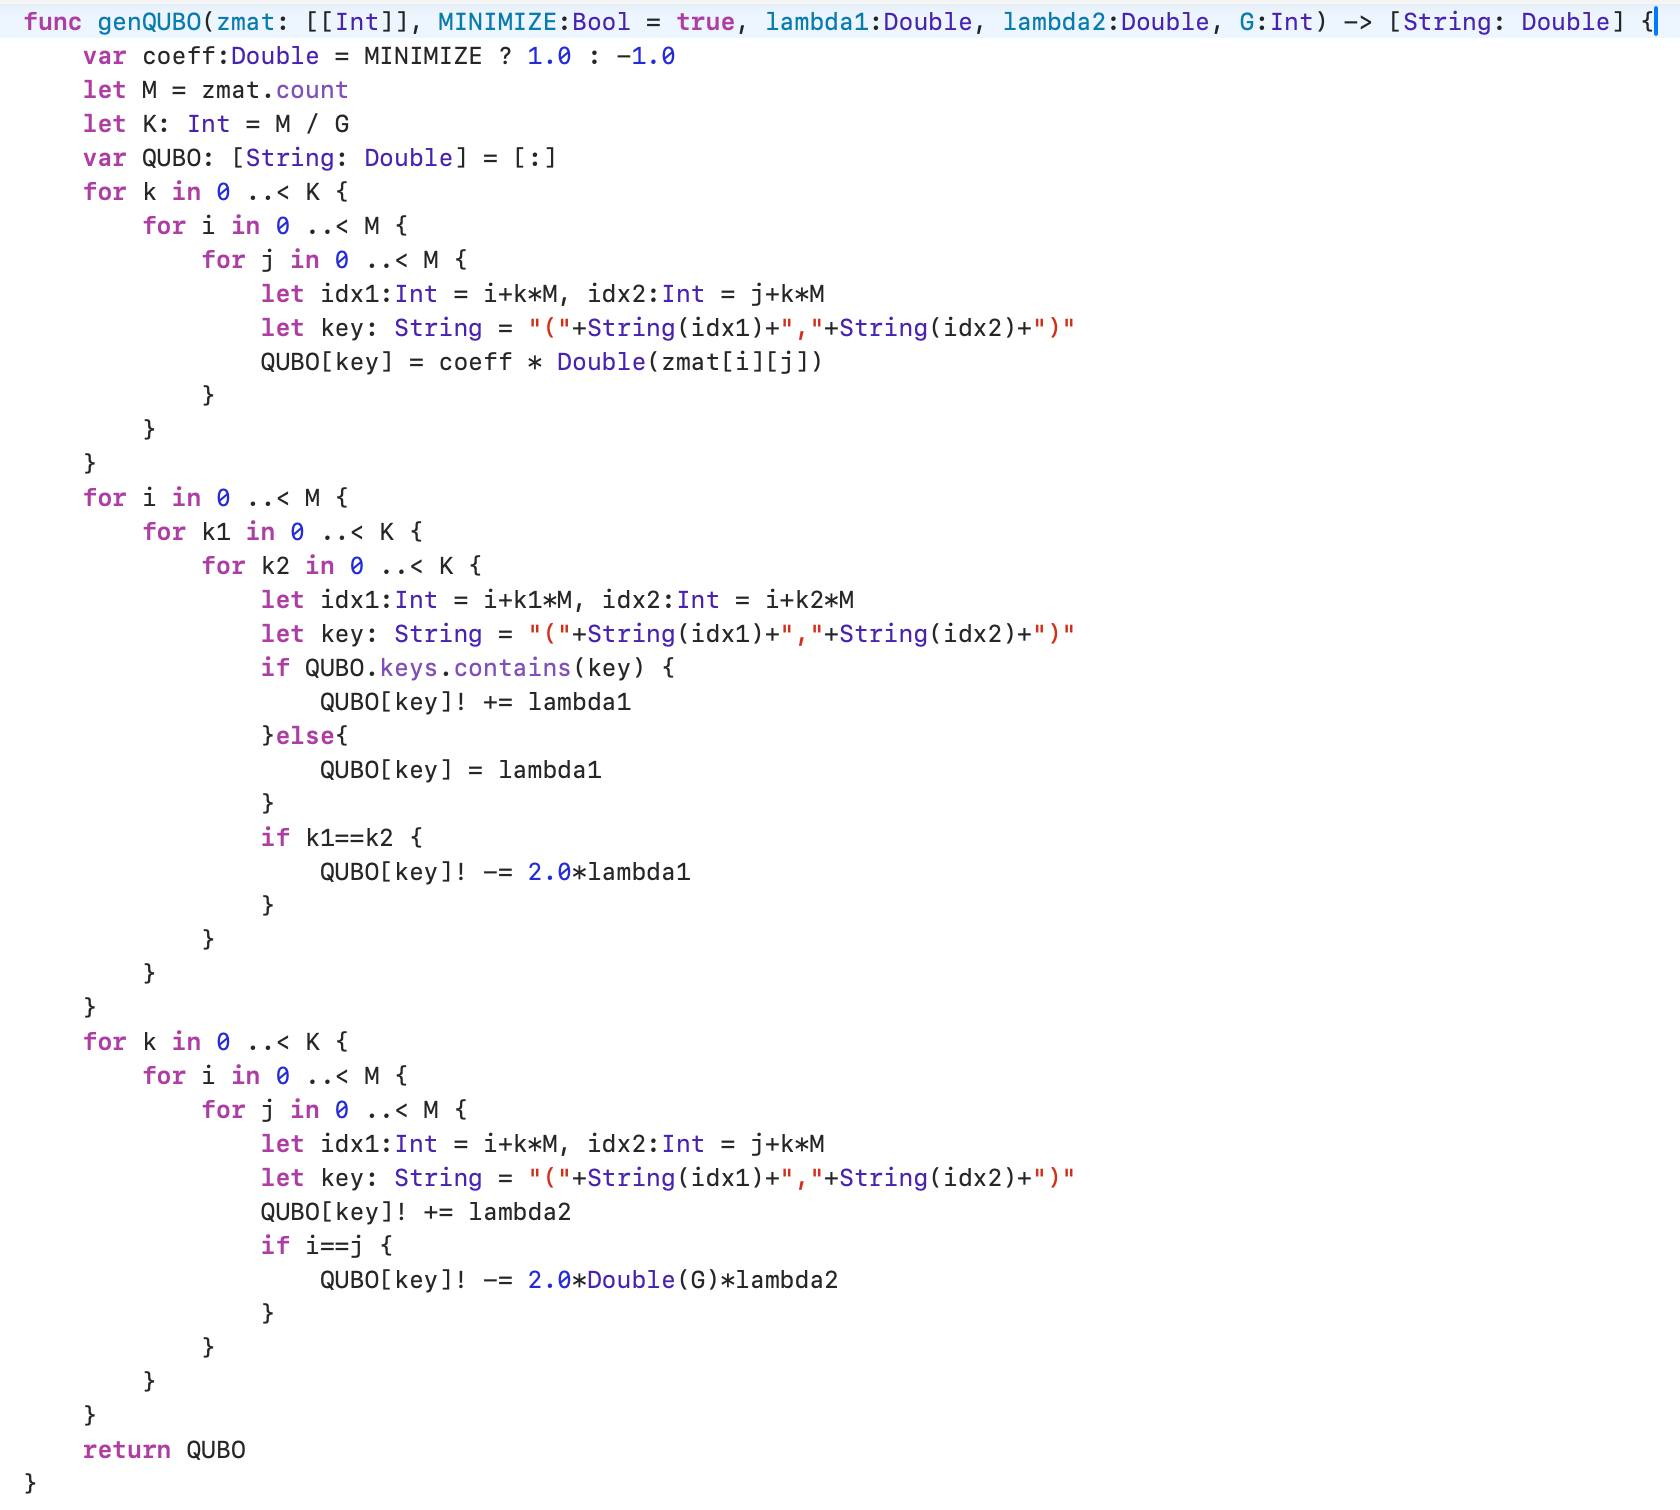
\includegraphics[width=\linewidth]{pictures/2025/03/20250328_160707_001.jpg}
\end{minipage}
\end{center}

\subsection*{2025年03月29日 08:30}
\addcontentsline{toc}{subsection}{2025年03月29日 08:30}

寝転んであれこれボーっと考えていたら、\#8クィーン を \#量子コンピュータ 用に定式化して解けるんじゃないか、という気になってきた。解を網羅する事は無くても、どれかの解に落ち着く事にはなるという気がする。（一段落したらやってみよう）

じゃあ、オセロはどう？という気にもなったけど、これは敷居が高いな。

むしろ三目並べ、五目並べはどうか。戦局の度にQUBOを作っては解かせる事になるのか？先ずは三目並べ（TicTacToe）かな。戦略はどんな形に定式化できるだろうか？８クイーンの次はTicTacToeに挑戦してみることにしよう。（量子コンピュータと対局できるぞ）


\url{https://ja.m.wikipedia.org/wiki/エイト・クイーン}



\url{https://en.m.wikipedia.org/wiki/Tic-tac-toe}



\paragraph{写真}
\begin{center}
\begin{minipage}{0.48\linewidth}
\centering
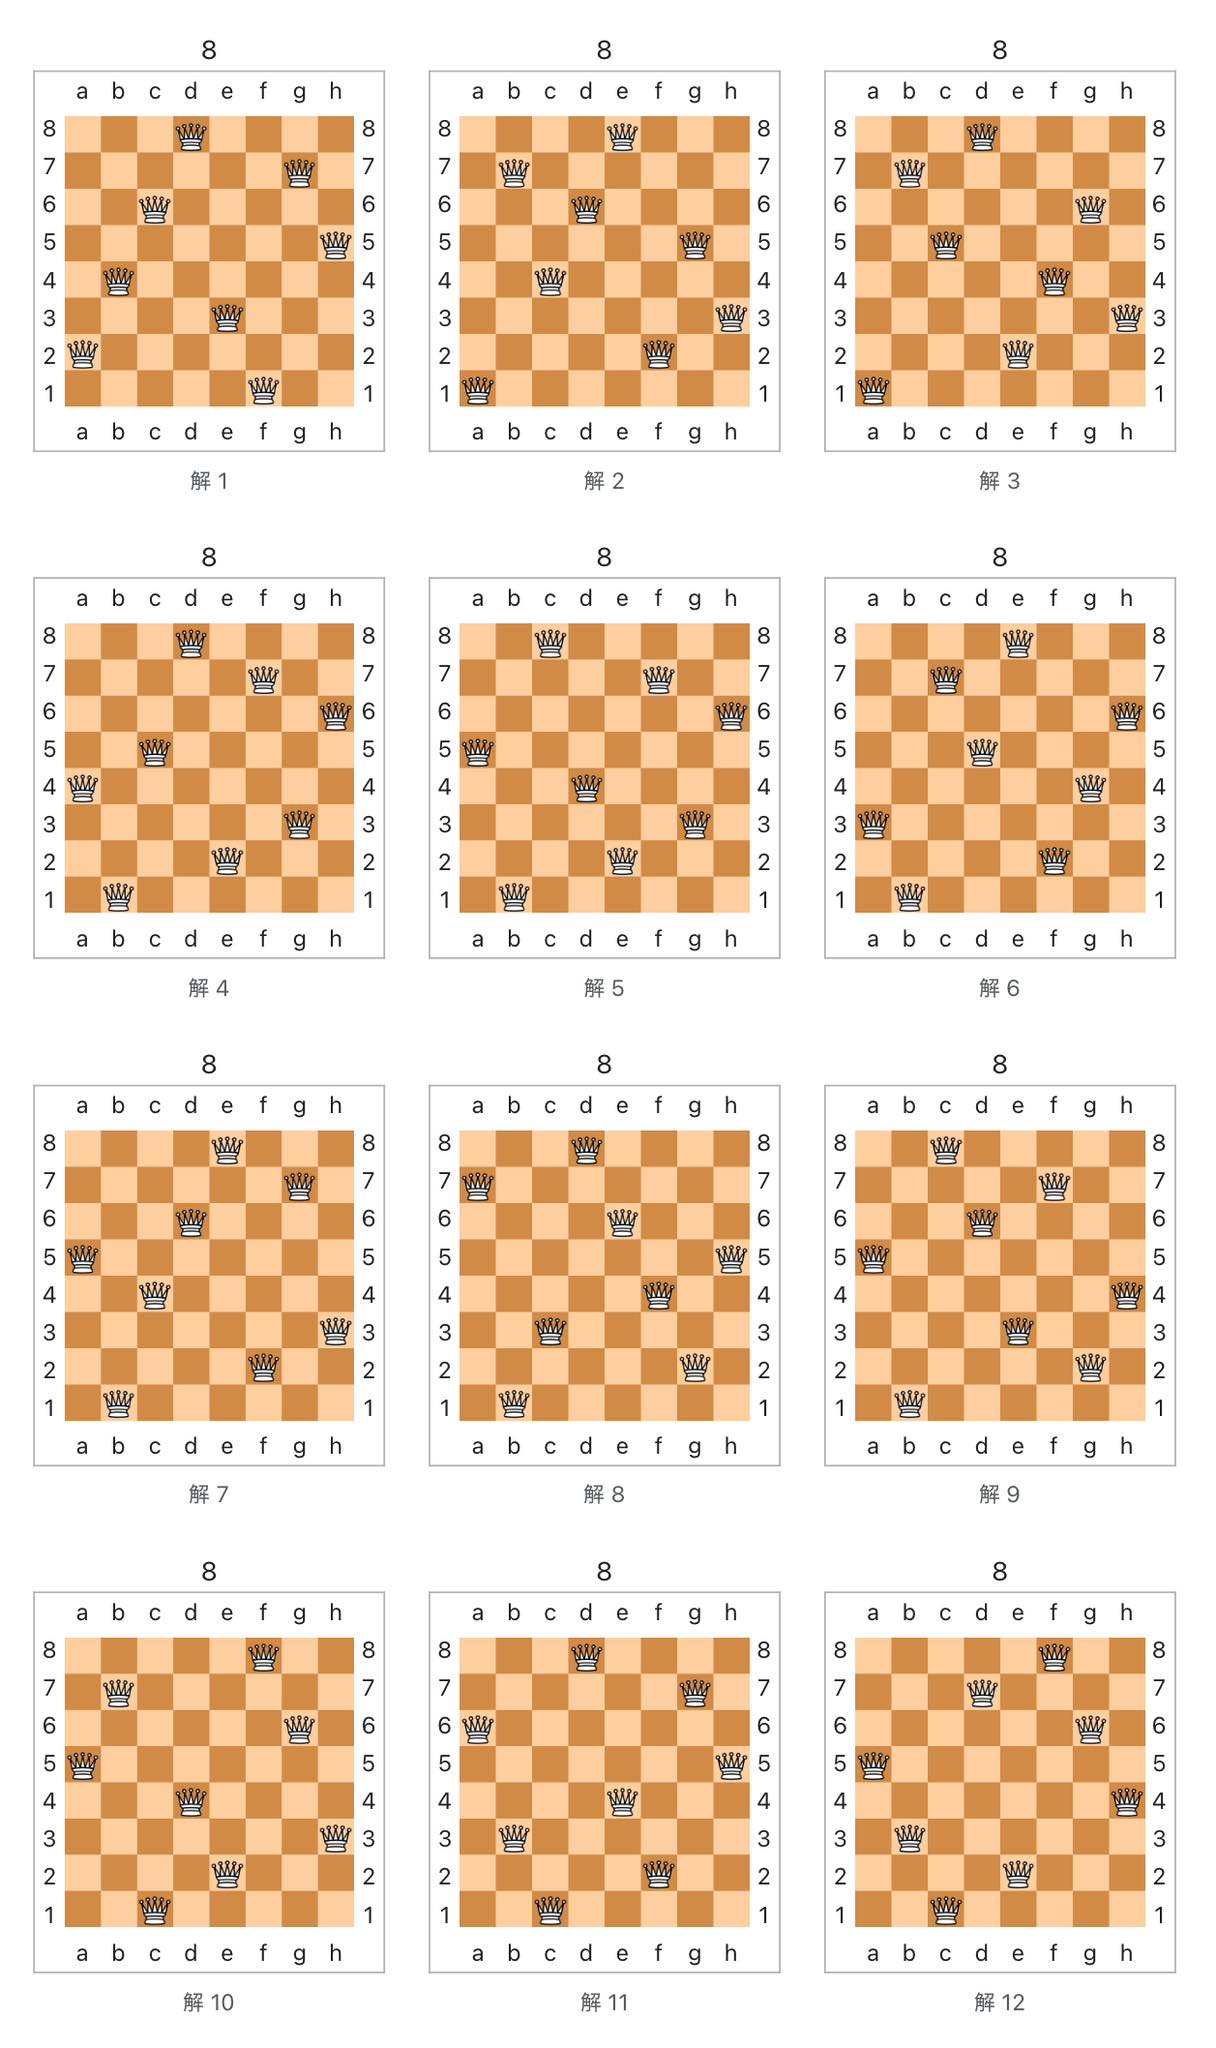
\includegraphics[width=\linewidth]{pictures/2025/03/20250329_083006_001.jpg}
\end{minipage}
\end{center}

\subsection*{2025年03月29日 10:27}
\addcontentsline{toc}{subsection}{2025年03月29日 10:27}

\#Python だったら \#numpy があって、\#行列 や \#ベクトル の計算を手軽にできるのですが、\#Swift のような場合（誰かが汎用的なものを作っているかもしれないけど）基本的に自前で用意する必要があります。

今回量子コンピュータのために用意したswiftによる行列計算の部分です。


転置行列のための \#extension（.transpose()）は、ネット上で拾ってきたものです。

\paragraph{写真}
\begin{center}
\begin{minipage}{0.48\linewidth}
\centering
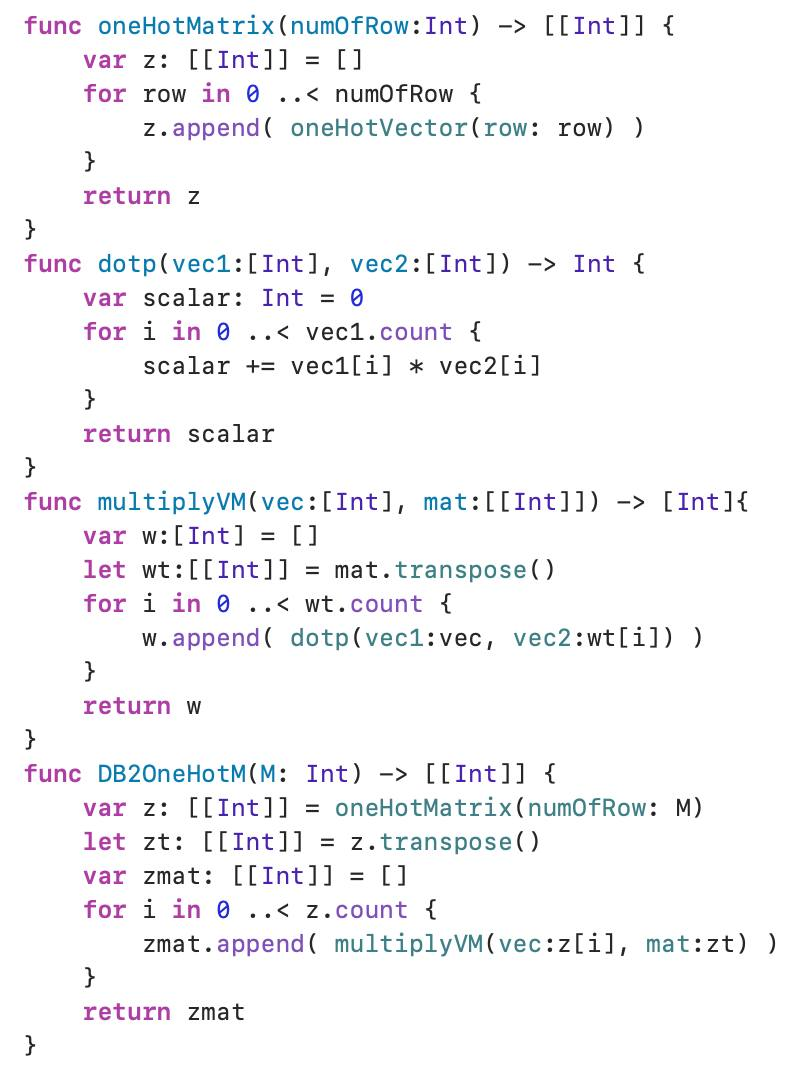
\includegraphics[width=\linewidth]{pictures/2025/03/20250329_102735_001.jpg}
\end{minipage}
\end{center}

\section{4月}

\subsection*{2025年04月03日 03:21}
\addcontentsline{toc}{subsection}{2025年04月03日 03:21}

\url{https://youtu.be/A61Yal78EQU}

\begin{center}
\href{https://youtu.be/A61Yal78EQU}{
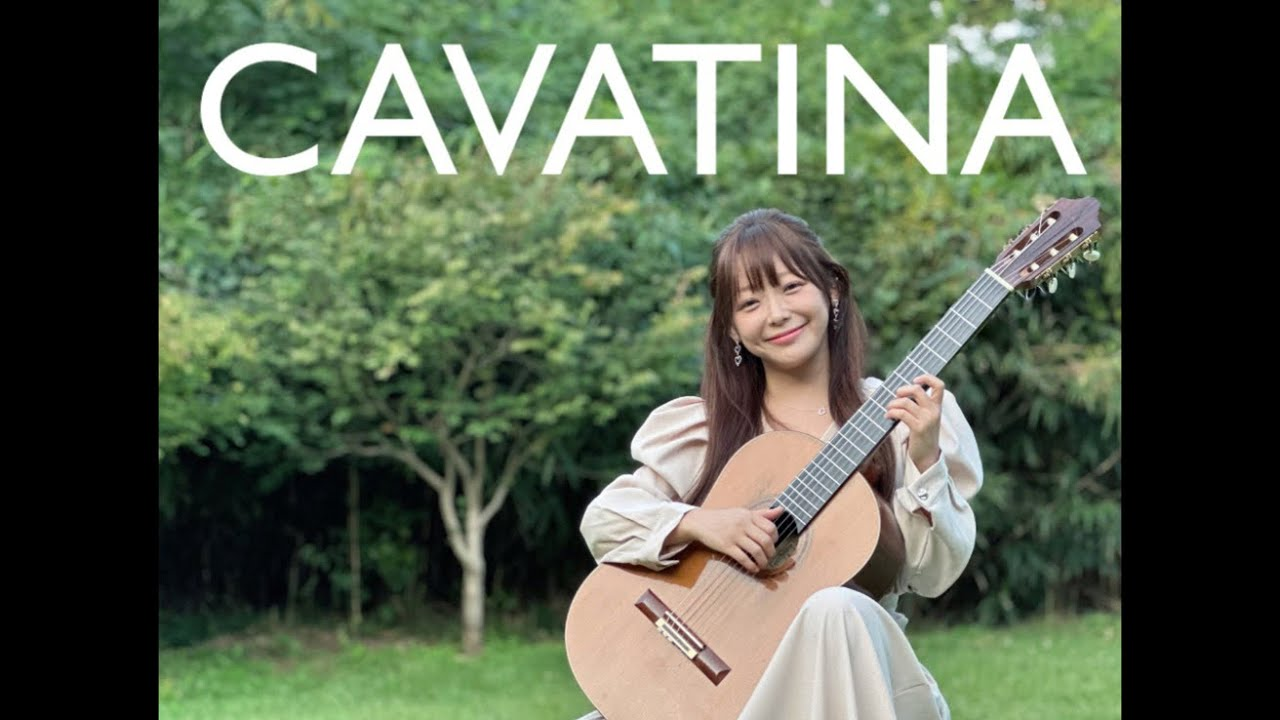
\includegraphics[width=0.48\linewidth]{pictures/youtube/2025/04/20250403_032129_youtube_001_A61Yal78EQU.jpg}
}
\end{center}



ハッシュタグがだんだんマインドマップになってくる。


比較的難しい曲らしいのですが、自分で演奏できたらいいな

こんな演奏したいと思います

\url{https://youtu.be/y_0pUbxMLCg}

\begin{center}
\href{https://youtu.be/y_0pUbxMLCg}{
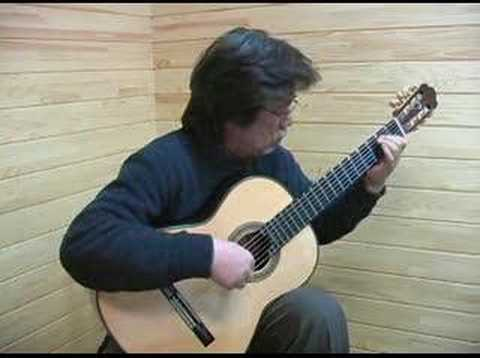
\includegraphics[width=0.48\linewidth]{pictures/youtube/2025/04/20250403_032129_youtube_002_y_0pUbxMLCg.jpg}
}
\end{center}




\#ディアハンター \#鹿狩り \#ベトナム戦争 \#ロシアンルーレット \#1960年代 \#アメリカ合衆国 \#若者 \#反戦 \#社会運動 \#ジョンウィリアムズ \#ロバートデニーロ \#友情 \#メリルストリーブ

\subsection*{2025年04月04日 01:05}
\addcontentsline{toc}{subsection}{2025年04月04日 01:05}

\paragraph{リンク}
\url{https://youtu.be/2HMJ1IGXumA}

\begin{center}
\href{https://youtu.be/2HMJ1IGXumA}{
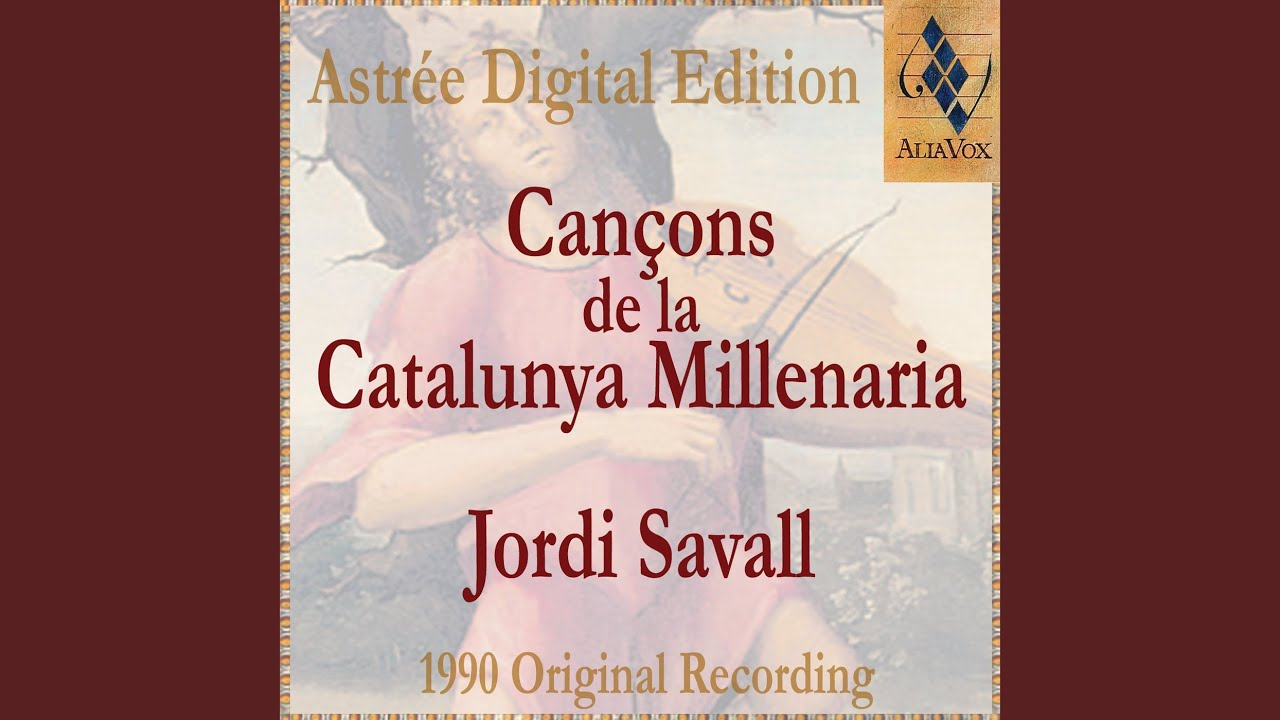
\includegraphics[width=0.48\linewidth]{pictures/youtube/2025/04/20250404_010531_youtube_001_2HMJ1IGXumA.jpg}
}
\end{center}

\subsection*{2025年04月04日 09:03}
\addcontentsline{toc}{subsection}{2025年04月04日 09:03}

\url{https://zenn.dev/luna_moonlight/articles/38de858bdc855f}




この方の記事は素晴らしい（＝とても参考になります）！

モデルを定式化して、\#QUBO を手作業で作って、コードとして実装するまで、順を追って詳しくまとめられている。（ \#QA4U で講義があったのと同じだと思ってよく見たら、この方もQA4Uを受けていた方との事でした）


この方のプログラムの中でとりわけ良いと思ったのは、 i 行j列という時のインデックスとQUBO行列のデータの並びのインデックスとの対応のつけ方が秀逸だと感じました。ix =i +N*jみたいなインデックスの変換を、プログラム上しなくてもよくなるからね。（真似させていただきます）


論理的にもよく整理されているので、この定式化にならって、私の \#８クィーン のプログラムもきちんと理論武装できる様に、これから見直してみようと思っています。（お世話になります）


\url{https://m.facebook.com/story.php?story_fbid=9394773580606719&id=100002225117991}




\#魔方陣 は3x3の各マスに1〜9の数値が入りますが、\#８クィーン の場合は8x8のマスに０or１が入るという訳です。また制約条件では、魔方陣が縦横斜めの数値の合計が同じ定数値（=15）になるのに対して、８クィーンの場合は、縦の列或いは横の行のそれぞれで、数値の合計は1（=1)でなければなりません。また斜め（対角のみならず他の斜めのラインでも）の合計は、どれも１以下（1又はゼロ）にならなければいけません。8クィーンで難しいと思うのは、この「1以下」という不等式の制約をQUBOに含めなければならない点です。


プログラムが正解の魔方陣を出してくるとは限らないという点について、まとめの所で触れられていますが、私の8クィーンのプログラムの場合でも、出てきた解の妥当性をチェックして、誤った出力（例えば対角に複数のクィーンが居たり）は除外してということをしてきました。もちろん未定定数lambdaの選び方には正解ヒット率を上げるためのknow howが有るはずですが、出力のチェックは、基本的には現在の \#量子コンピュータ に必要な付き合い方なのかなと思ったりしています。


\#TeX による数式が長くなると、数式の右の方が画面の外にはみ出して読めなくなってしまっている。（でも、QA4Uを受けていたので見えなくてもOkです）

\subsection*{2025年04月04日 21:33}
\addcontentsline{toc}{subsection}{2025年04月04日 21:33}

\paragraph{リンク}
\url{https://youtu.be/To8bv4bAC4E}

\begin{center}
\href{https://youtu.be/To8bv4bAC4E}{
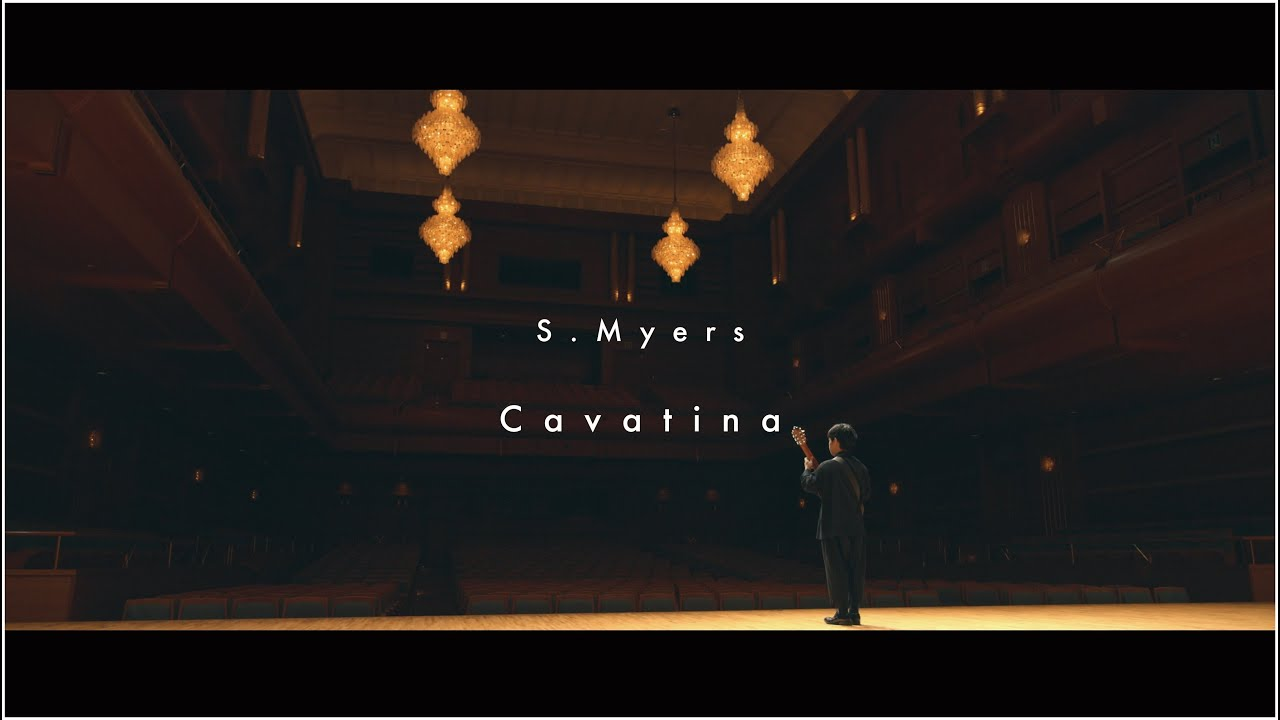
\includegraphics[width=0.48\linewidth]{pictures/youtube/2025/04/20250404_213332_youtube_001_To8bv4bAC4E.jpg}
}
\end{center}

\subsection*{2025年04月04日 22:37}
\addcontentsline{toc}{subsection}{2025年04月04日 22:37}

\url{https://youtu.be/RmeKARDSBkg}

\begin{center}
\href{https://youtu.be/RmeKARDSBkg}{

\includegraphics[width=0.48\linewidth]{pictures/youtube/2025/04/20250404_223729_youtube_001_RmeKARDSBkg.jpg}
}
\end{center}




マーラーのアダージェットをギターで演奏するのも「凄い」けど、これもまたギターの可能性を大きく感じさせる演奏ですね。（アダージェット同様、自分で演奏しようなどとは思はない。）


オリジナルの曲は \#キースジャレット の \#ケルンコンサート ですが、これはそもそもキースが舞台の上の一台のピアノに向かって、その時の即興で演奏しているとても長い曲です。これは、そのうちのパート２の終わりの方でなかったかな（LPレコード二枚目の裏だった？表だった？）。パート１の出だしの辺りはTVでCMなどに使われたりしているのでよく耳にします。


キースのピアノも「凄い」けど、即興演奏を楽譜にした人も「すごい」。そしてそれをギター用に編曲した人（Manuel Barruecoという方らしい）も「凄い」し、何と言ってもギターを自在に駆使して演奏している \#村治佳織 氏の表現力も「すごい」です。ごまかさない丁寧な演奏表現が好きです。

\subsection*{2025年04月04日 22:41}
\addcontentsline{toc}{subsection}{2025年04月04日 22:41}

\paragraph{リンク}
\url{https://youtu.be/6_2cbCrTrIM}

\begin{center}
\href{https://youtu.be/6_2cbCrTrIM}{
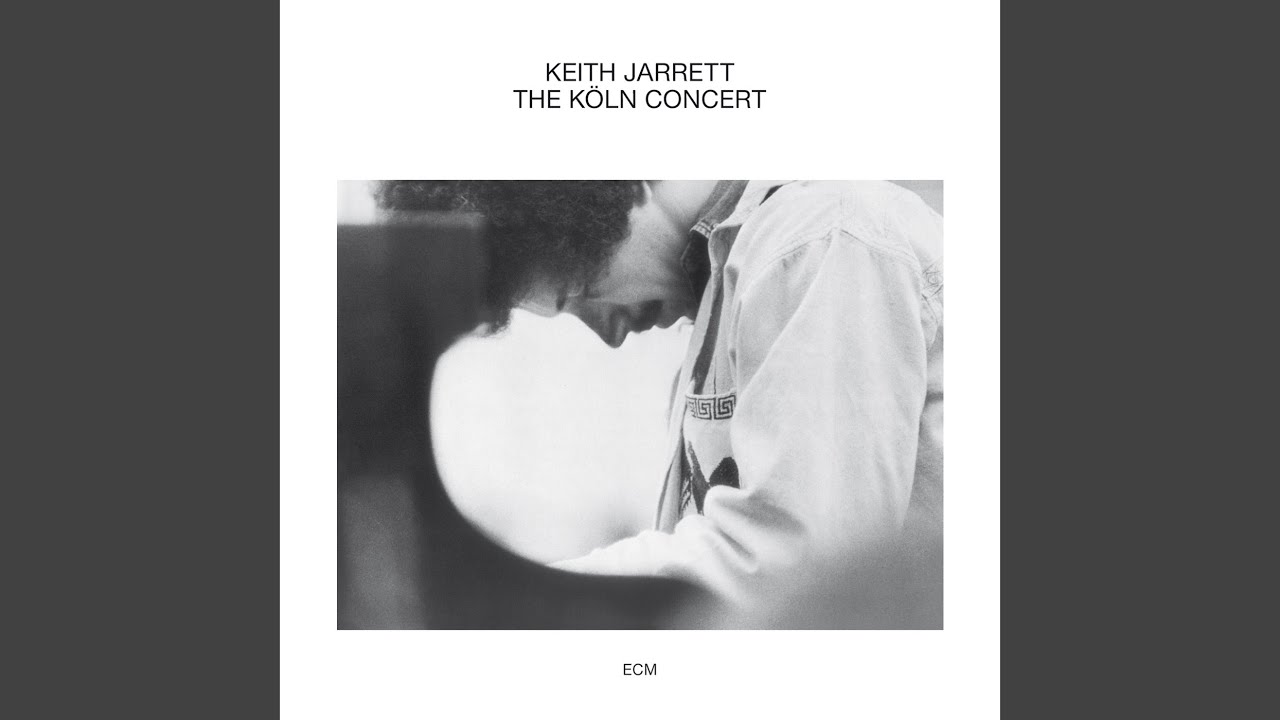
\includegraphics[width=0.48\linewidth]{pictures/youtube/2025/04/20250404_224141_youtube_001_6_2cbCrTrIM.jpg}
}
\end{center}

\subsection*{2025年04月05日 01:08}
\addcontentsline{toc}{subsection}{2025年04月05日 01:08}

\paragraph{リンク}
\url{https://youtu.be/9Bbm-7vdlbs}

\begin{center}
\href{https://youtu.be/9Bbm-7vdlbs}{
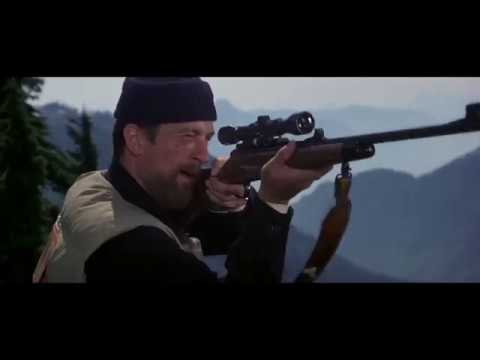
\includegraphics[width=0.48\linewidth]{pictures/youtube/2025/04/20250405_010820_youtube_001_9Bbm-7vdlbs.jpg}
}
\end{center}

\subsection*{2025年04月05日 01:23}
\addcontentsline{toc}{subsection}{2025年04月05日 01:23}

\paragraph{リンク}
\url{https://youtu.be/deis_6yXWdA}

\begin{center}
\href{https://youtu.be/deis_6yXWdA}{
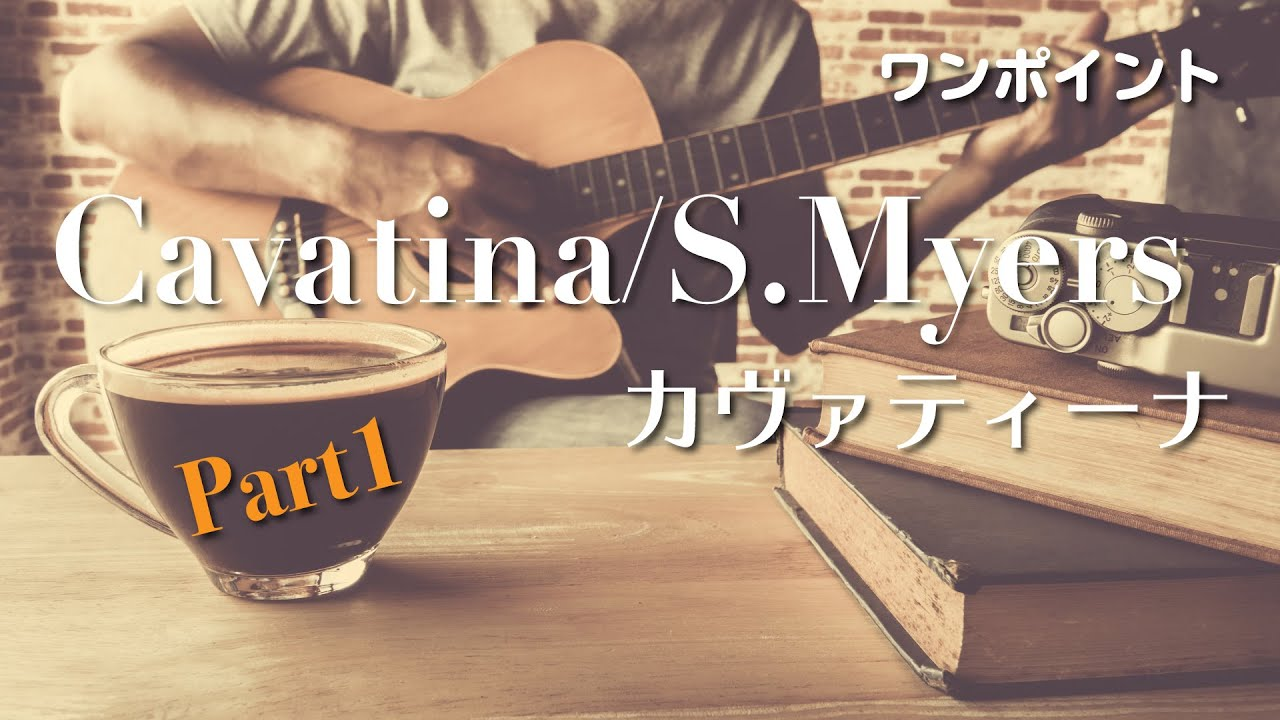
\includegraphics[width=0.48\linewidth]{pictures/youtube/2025/04/20250405_012327_youtube_001_deis_6yXWdA.jpg}
}
\end{center}

\subsection*{2025年04月05日 01:23}
\addcontentsline{toc}{subsection}{2025年04月05日 01:23}

\paragraph{リンク}
\url{https://youtu.be/P6FzXOKaylQ}

\begin{center}
\href{https://youtu.be/P6FzXOKaylQ}{
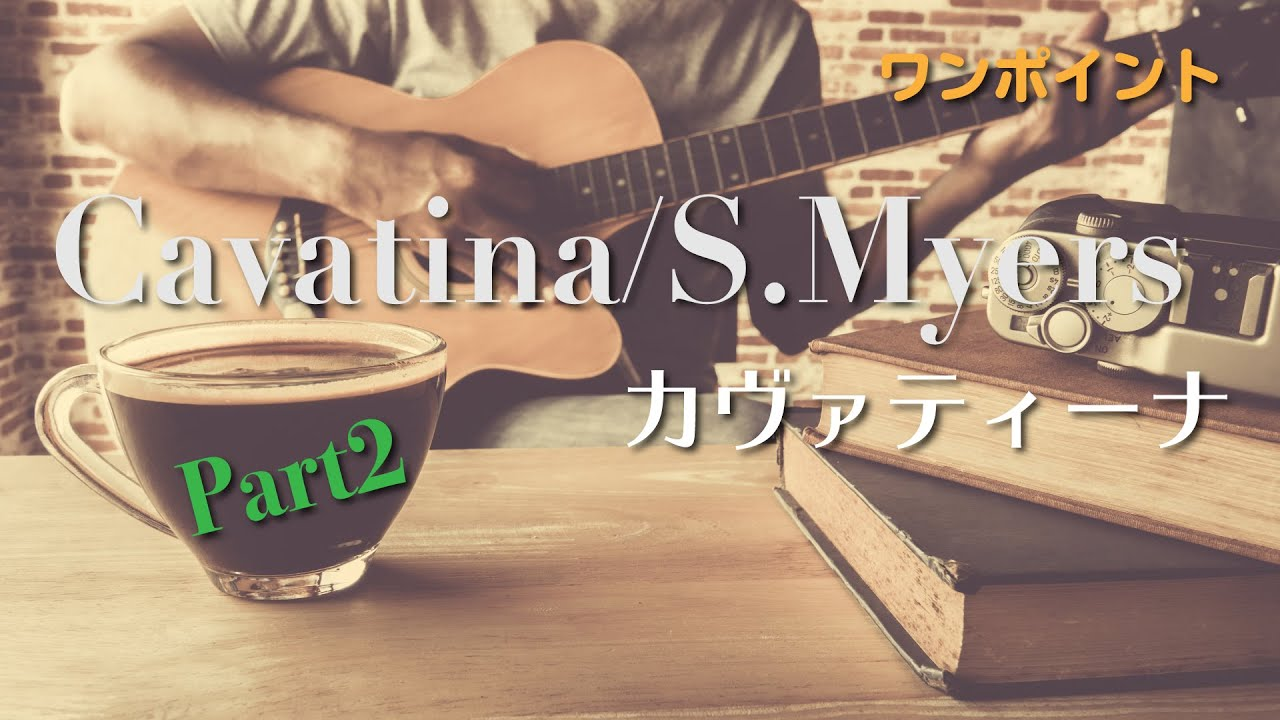
\includegraphics[width=0.48\linewidth]{pictures/youtube/2025/04/20250405_012359_youtube_001_P6FzXOKaylQ.jpg}
}
\end{center}

\subsection*{2025年04月07日 02:07}
\addcontentsline{toc}{subsection}{2025年04月07日 02:07}

\url{https://youtu.be/xv8b96c61Rw}

\begin{center}
\href{https://youtu.be/xv8b96c61Rw}{
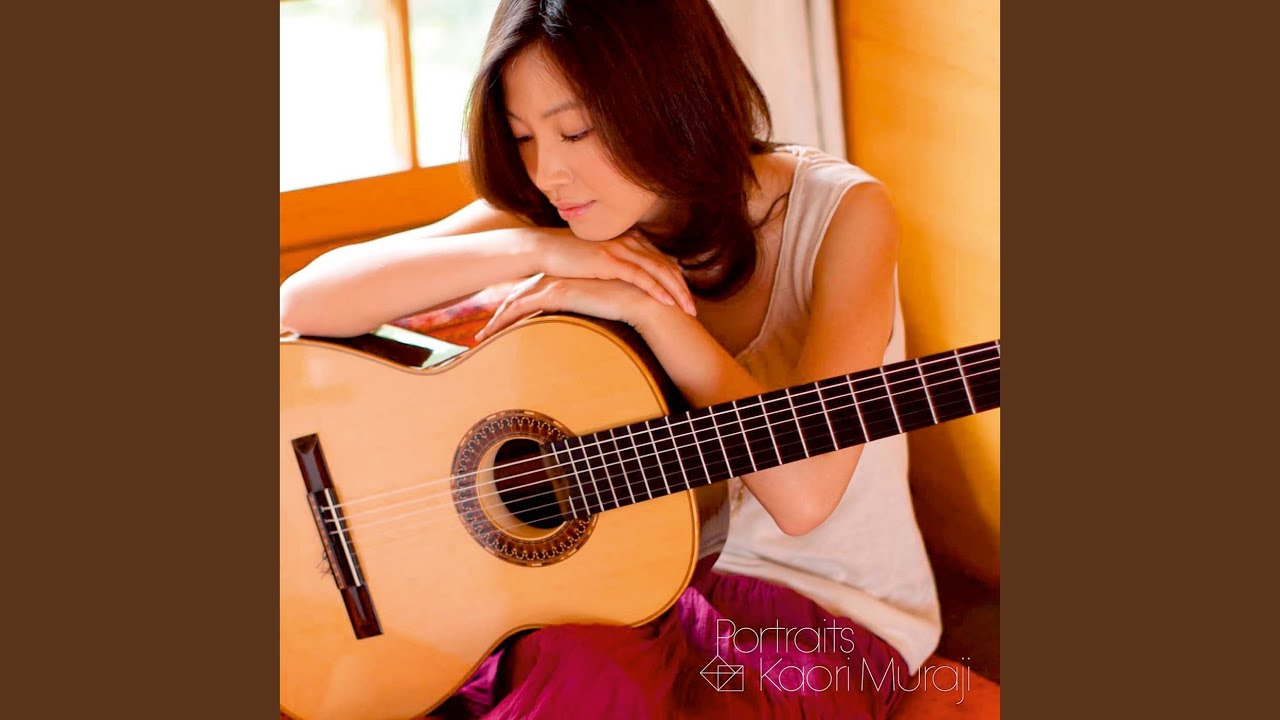
\includegraphics[width=0.48\linewidth]{pictures/youtube/2025/04/20250407_020716_youtube_001_xv8b96c61Rw.jpg}
}
\end{center}




ガーシュインもいいなあ。武満徹氏の編曲ですか。楽譜を手に入れてみる？（私に武満を弾けるわけないよ）やめときます。

\subsection*{2025年04月07日 23:02}
\addcontentsline{toc}{subsection}{2025年04月07日 23:02}

\url{https://github.com/smat1957/QA4U/tree/main/EightQueen}




三月末からこの一週間ほど,ああでもない,こうでもないと格闘してきた, \#量子コンピュータ による \#8クィーン の解法プログラム（ \#Python ）が,ある程度満足できる形になったので, \#GitHub に（少なくとも自分にだけは分かる説明文書を添えて）一式置いてきました.


説明文書は8queen.pdf.

PDFを書いた \#TeX のソース（8queen.tex）も一緒に置いている.

Pythonのプログラムは2つ置いていますが,QUBOの表現が異なるものを,それぞれのプログラムで試したものです. num\_reads=10000回程度試行すれば,どちらのプログラムも12個の基本解を出力してきます.


GitHubは私にとっては備忘録になってしまっています. GitHubのReadMeみたいなのは用意していないけれど,多くの場合にTeXで書いた説明用のPDF文書を同梱する様にしています. 自分のPCの中に保存したままにしておくと,いつのまにか何処に何があったかも忘れてしまって（歳とっただけか）.しかもこれがPCを更新したりなんかすると,全てが綺麗になくなってしまいますから.最近では,一段落したものはアップロードしておくことにしています.

\paragraph{写真}
\begin{center}
\begin{minipage}{0.48\linewidth}
\centering
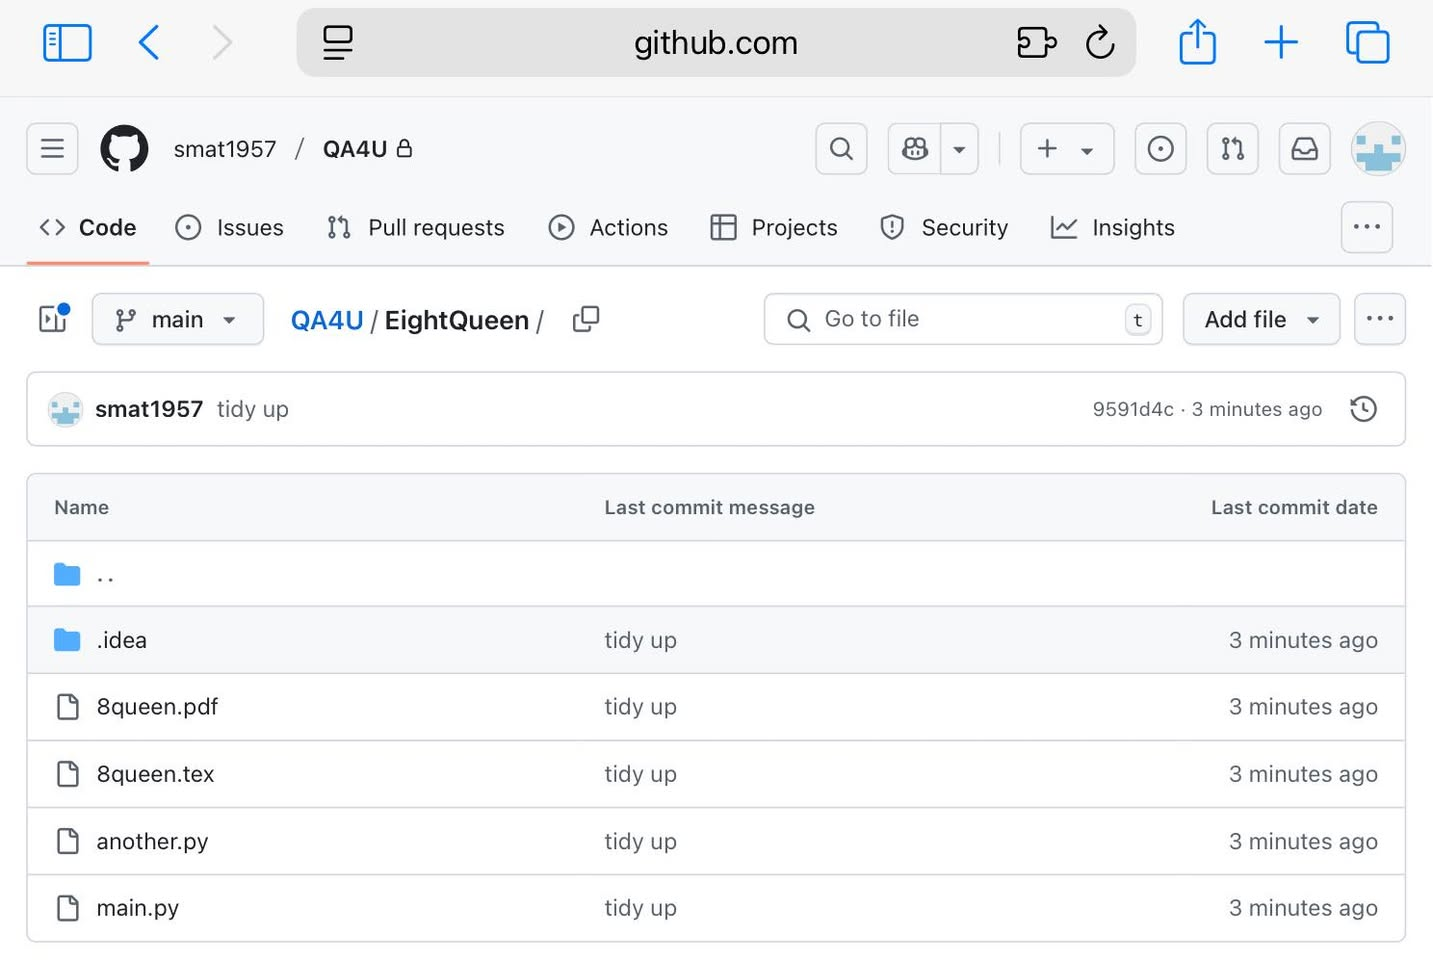
\includegraphics[width=\linewidth]{pictures/2025/04/20250407_230214_001.jpg}
\end{minipage}
\end{center}

\subsection*{2025年04月08日 23:20}
\addcontentsline{toc}{subsection}{2025年04月08日 23:20}

この演奏は武満徹氏の編曲によるものではありません！

聞き慣れない編曲なので, ちょっと新鮮に聞こえます

Stephanie Jonesさんの演奏, 良いですね、とっても


\url{https://youtu.be/inc7THXyJ1o}

\begin{center}
\href{https://youtu.be/inc7THXyJ1o}{
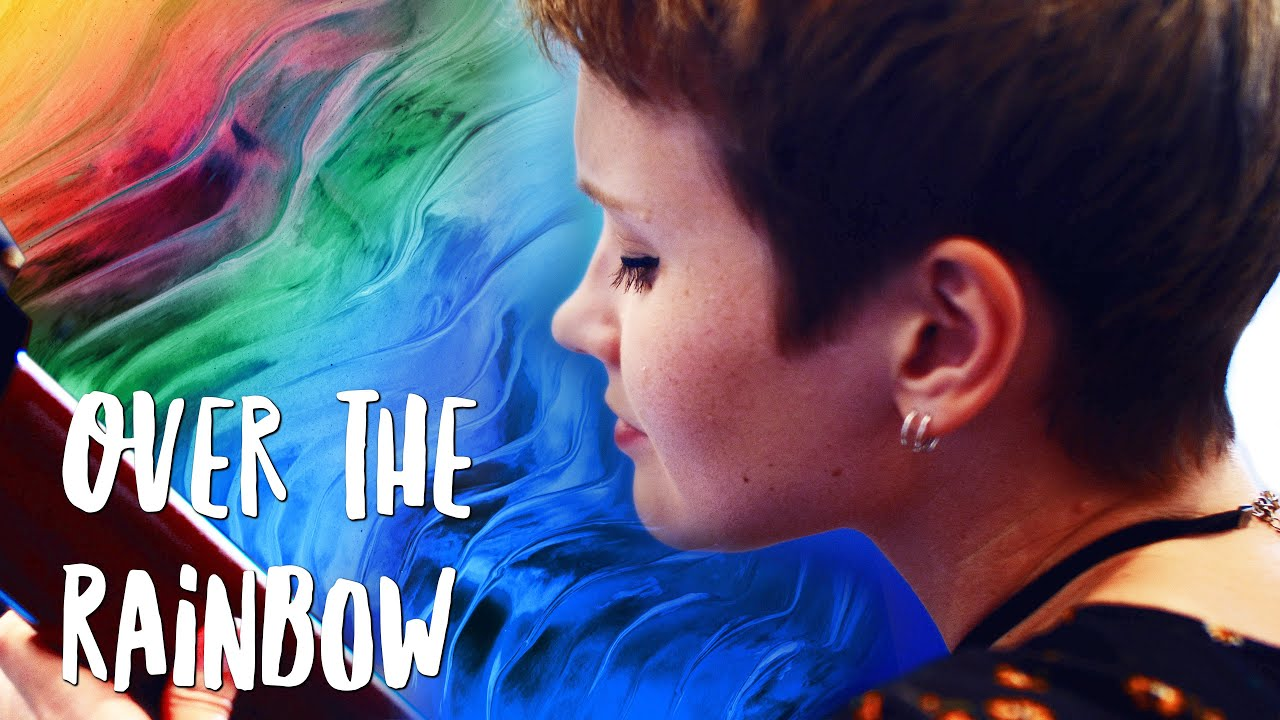
\includegraphics[width=0.48\linewidth]{pictures/youtube/2025/04/20250408_232031_youtube_001_inc7THXyJ1o.jpg}
}
\end{center}




編曲は、David Jaggs氏, 楽譜は以下で購入できるらしい

\url{http://www.davidjaggs.com/easy-listening.html}



或いはAmazonでも 

\url{https://amzn.asia/d/1uwF89i}



これ（ 

\url{https://youtu.be/jmq-628yiJI}

\begin{center}
\href{https://youtu.be/jmq-628yiJI}{
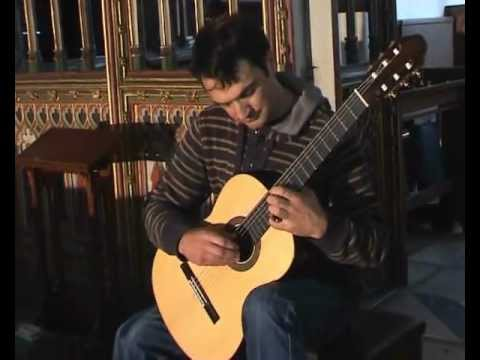
\includegraphics[width=0.48\linewidth]{pictures/youtube/2025/04/20250408_232031_youtube_002_jmq-628yiJI.jpg}
}
\end{center}

 ）は編曲者自身による演奏です。同じ楽譜でも、誰でもStephanieさんの様なセンスで演奏できるって訳じゃないんだなぁ。


一方, 武満徹氏編曲によるこの曲の演奏なら色々ありますが、例えば


\url{https://www.facebook.com/100002225117991/posts/25693913046932847/}



\subsection*{2025年04月11日 21:06}
\addcontentsline{toc}{subsection}{2025年04月11日 21:06}

次はこの曲（エストレリータ、マヌエル・ポンセ作曲）をやってみようと考えているところです。いろんな楽器で演奏されている様ですが、オリジナルは何の曲なんでしょうか？（歌曲かな？）


\url{https://youtu.be/VVptQ91LWYw}

\begin{center}
\href{https://youtu.be/VVptQ91LWYw}{
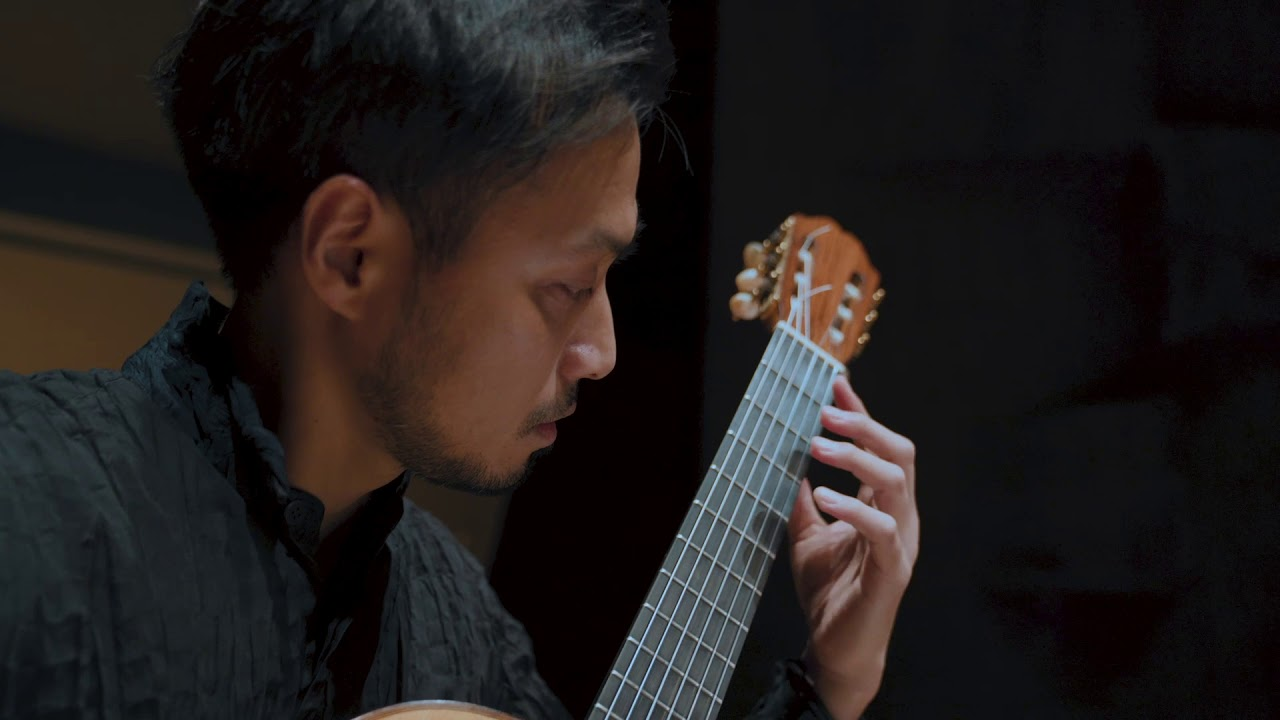
\includegraphics[width=0.48\linewidth]{pictures/youtube/2025/04/20250411_210612_youtube_001_VVptQ91LWYw.jpg}
}
\end{center}




前半の繰り返し、後半の繰り返しとあって、従って短い曲（現代ギター社「てんこもりVol2」ホセ・ルイス・ゴンザレス編）ですので、何とかならないかなと思って、少し運指を追ってみました。左手の指ではじく装飾音が難しそうだけど、何とかなりそうか？（＝ごまかせそうか？）と思いながらも、一抹の不安がよぎります。それはつまり、概して「オシャレに」弾けるだろうか？という問題です。Youtubeで曲の演奏を解説している方も、メトロノーム通りだと「ダサイ」とおっしゃっています。でも、悩むのはとにかく全体を通せる様になってからだ、と思う事にしました。（山に登る前に諦めていたら、結局どの山にも登らずに、評論するだけで終わってしまうから。）


他の方（Leonardo Bravo）による編曲もある（←楽譜欲しい）

\url{https://youtu.be/LVkyT5xcQsU}

\begin{center}
\href{https://youtu.be/LVkyT5xcQsU}{
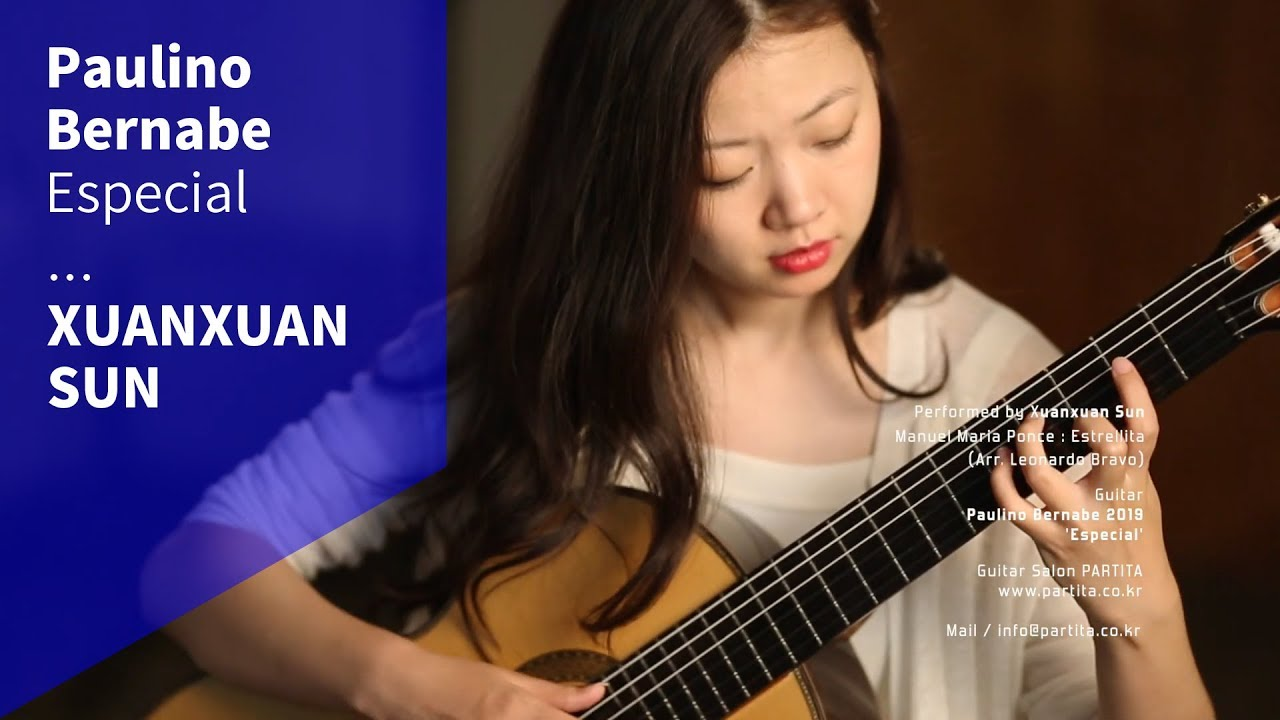
\includegraphics[width=0.48\linewidth]{pictures/youtube/2025/04/20250411_210612_youtube_002_LVkyT5xcQsU.jpg}
}
\end{center}




\#ポンセ \#クラシックギター \#エストレリータ \#classicalguitar \#ManuelMPonce  \#Estrellita \#小さな星

\subsection*{2025年04月11日 21:06}
\addcontentsline{toc}{subsection}{2025年04月11日 21:06}

\paragraph{リンク}
\url{https://youtu.be/UkomY5S6hHo}

\begin{center}
\href{https://youtu.be/UkomY5S6hHo}{
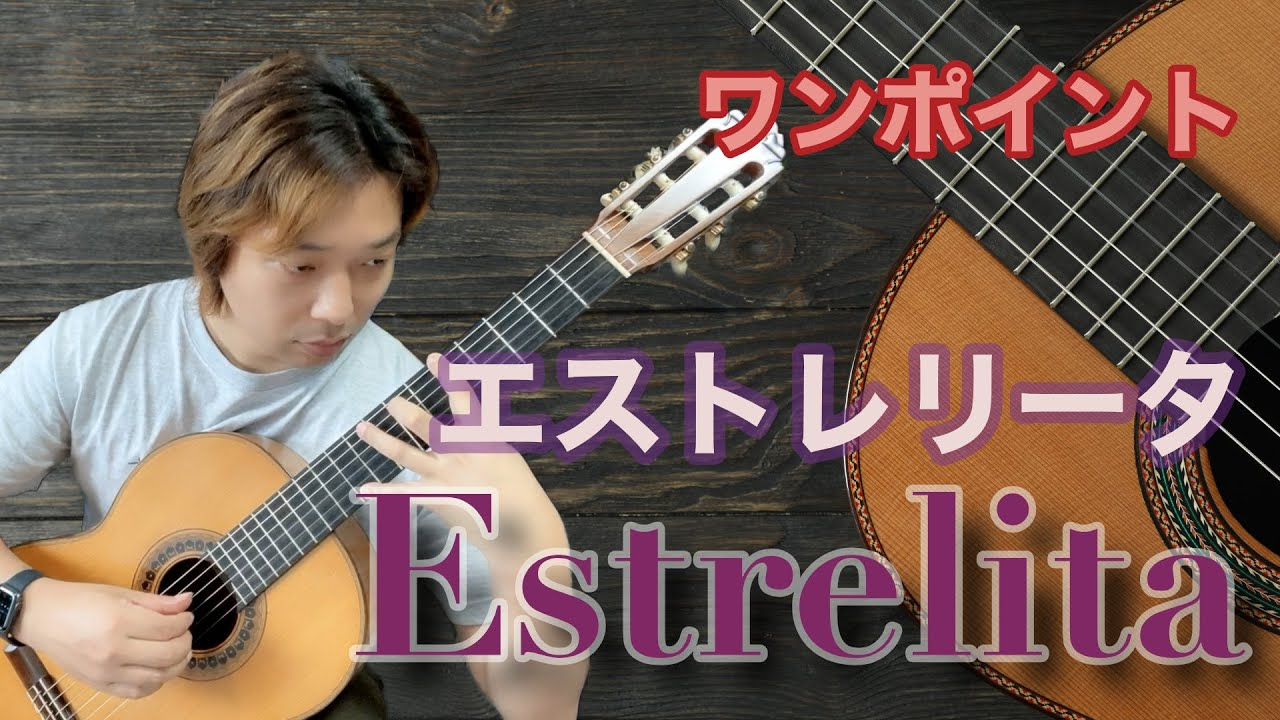
\includegraphics[width=0.48\linewidth]{pictures/youtube/2025/04/20250411_210649_youtube_001_UkomY5S6hHo.jpg}
}
\end{center}

\subsection*{2025年04月12日 12:05}
\addcontentsline{toc}{subsection}{2025年04月12日 12:05}

泉鏡花、徳田秋声、室生犀星の3人の小説家、詩人をさして「金沢の三文豪」と言うらしい。（これは聞いたことがある様な気がする）


また、石川県出身で同じ年に生まれた、西田幾多郎、鈴木大拙（本名・貞太郎）、藤岡作太郎、三人のことを「加賀の三たろう」と呼ぶらしい。（初耳です！）


\url{https://youtu.be/k5aHUlu-L84}

\begin{center}
\href{https://youtu.be/k5aHUlu-L84}{
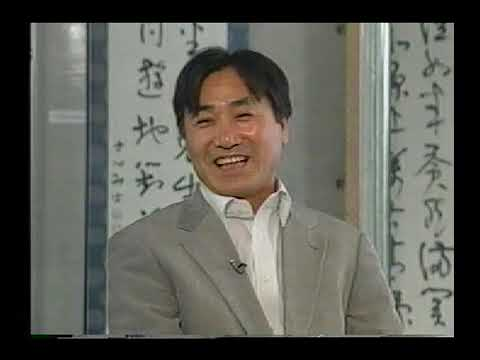
\includegraphics[width=0.48\linewidth]{pictures/youtube/2025/04/20250412_120530_youtube_001_k5aHUlu-L84.jpg}
}
\end{center}




「金沢ふるさと偉人館」が、金沢市の歌劇座（旧くは観光会館）の裏あたりに、

「泉鏡花記念館」が、金沢市下新町（旧くは旧森八本店裏）に、

「徳田秋声記念館」が、金沢市東山（浅野川の梅ノ橋あたり）に、

「室生犀星記念館」が、金沢市千日町に、

「西田幾多郎記念哲学館」（安藤忠雄氏設計による）は、石川県かほく市に、

「鈴木大拙館」（谷口吉生氏設計による）は、金沢市の本多の森に、

「谷口吉生記念建築館」が、金沢市の寺町に、

「金沢文芸館」（五木寛之氏の著作等を取集展示）が、金沢市尾張町（橋場町交差点で旧くは銀行）に、

「金沢湯涌夢二館」（竹久夢二氏の作品等を展示）が、金沢市湯涌町に、

ある。

\subsection*{2025年04月13日 14:29}
\addcontentsline{toc}{subsection}{2025年04月13日 14:29}

\paragraph{リンク}
\url{https://youtu.be/rMpsrVfPcnw}

\begin{center}
\href{https://youtu.be/rMpsrVfPcnw}{
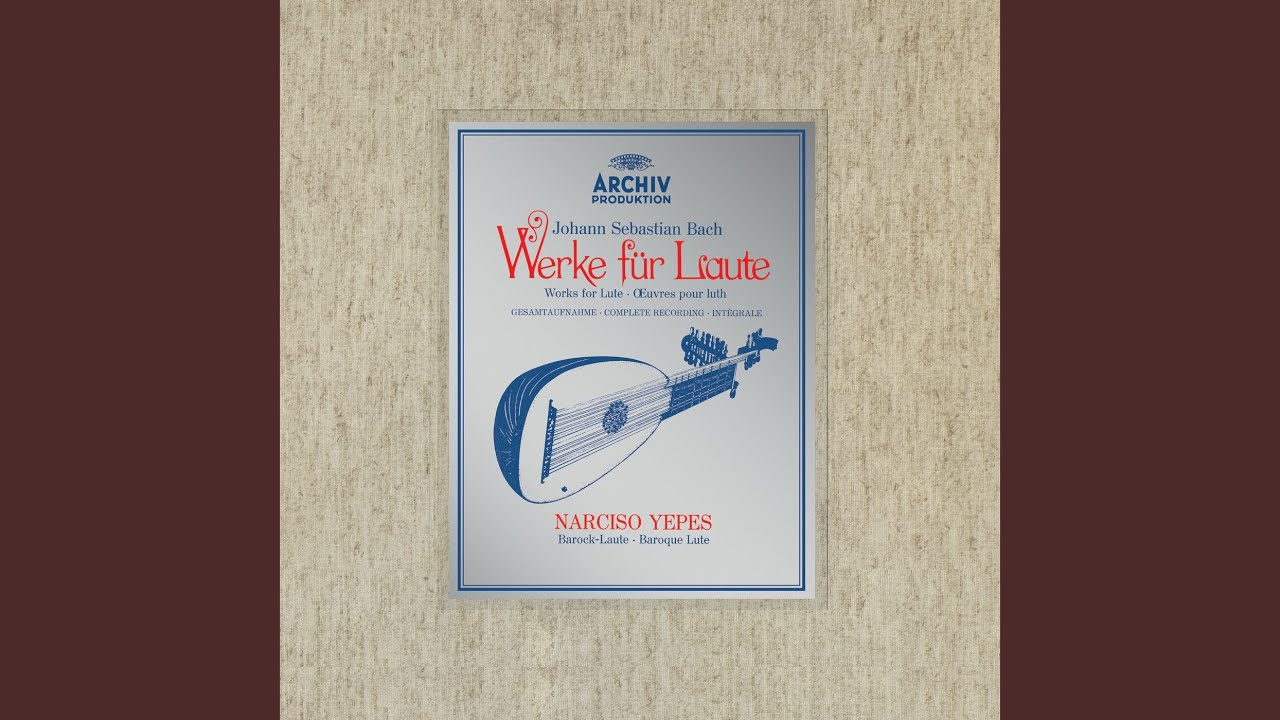
\includegraphics[width=0.48\linewidth]{pictures/youtube/2025/04/20250413_142958_youtube_001_rMpsrVfPcnw.jpg}
}
\end{center}

\subsection*{2025年04月15日 01:40}
\addcontentsline{toc}{subsection}{2025年04月15日 01:40}

\url{https://github.com/smat1957/QA4U/tree/main/KnapSack}




\#ナップザック問題 は、この分野では古典的なテーマなので、一度は解く事に挑戦しなければと思っていたところでした。この記事(

\url{https://qiita.com/farcpan/items/5c2053ce1fd79e644eef}

 ）には、slack変数 を用いた \#不等式による制約 の付け方について分かりやすく書かれていたので、大いに参考にさせてもらいました。


ただ（惜しまれるのは）この記事では \#ハミルトニアン の形を示すにとどめられていて、具体的な問題に対応した場合の \#QUBO から先のコードについては触れられていません。「ハミルトニアンの恰好まで出しているので、後はやってちょうだいね」と言われている様な気もします。ので、とにかく私がその続き（具体的なコード）を用意する事にしましょう。（解けるのかどうなのかはハミルトニアンとは別の話） \#量子コンピュータ がどんな答えを出すのか、実はちょっと気になっていたので。


という事で、作成したプログラムのソースと \#PDF ドキュメント、それとそのPDFドキュメントを作った際の \#TeX のソース、この三つを、いつもの \#GitHub （冒頭記載）に置いてきました。


実行してみると期待した様な結果が得られました。

試している問題は「5個の荷物から選んで、最大容量12のナップザックに積むときに、各荷物が持っている価値金額の合計が最大になる組み合わせ」を求めています。（制約条件は、ナップザックに入れる荷物の容量の総和が「12以下」）

\#Openjij のシミュレータ \#SASampler() でnum\_reads=100にして実施したところ、、、（詳細はGitHubに）

\paragraph{写真}
\begin{center}
\begin{minipage}{0.48\linewidth}
\centering
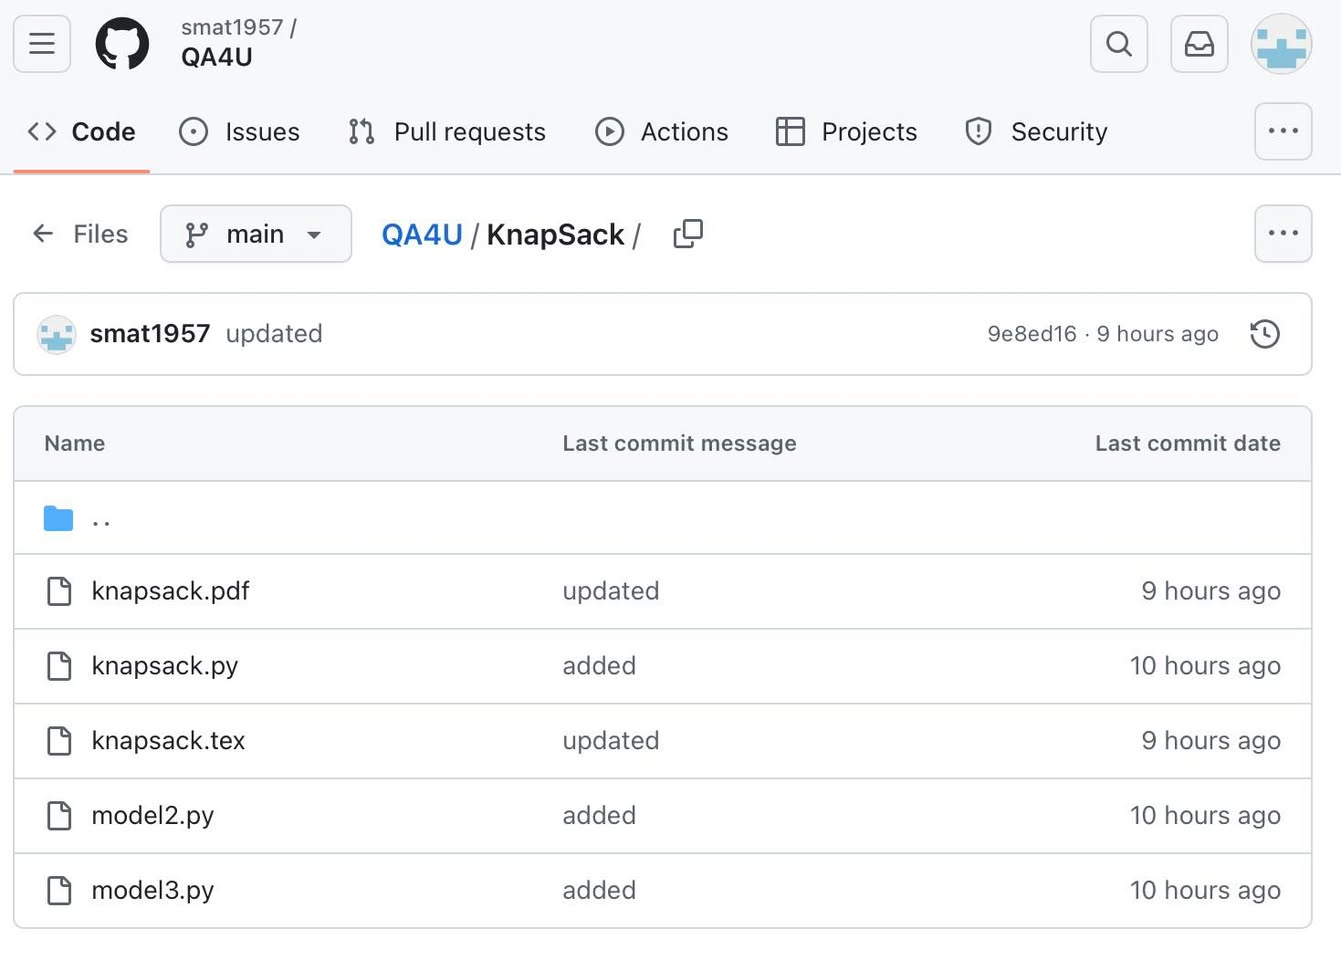
\includegraphics[width=\linewidth]{pictures/2025/04/20250415_014034_001.jpg}
\end{minipage}
\end{center}

\subsection*{2025年04月15日 11:38}
\addcontentsline{toc}{subsection}{2025年04月15日 11:38}

\paragraph{リンク}
\url{https://youtu.be/QR50OtY7fhY}

\begin{center}
\href{https://youtu.be/QR50OtY7fhY}{
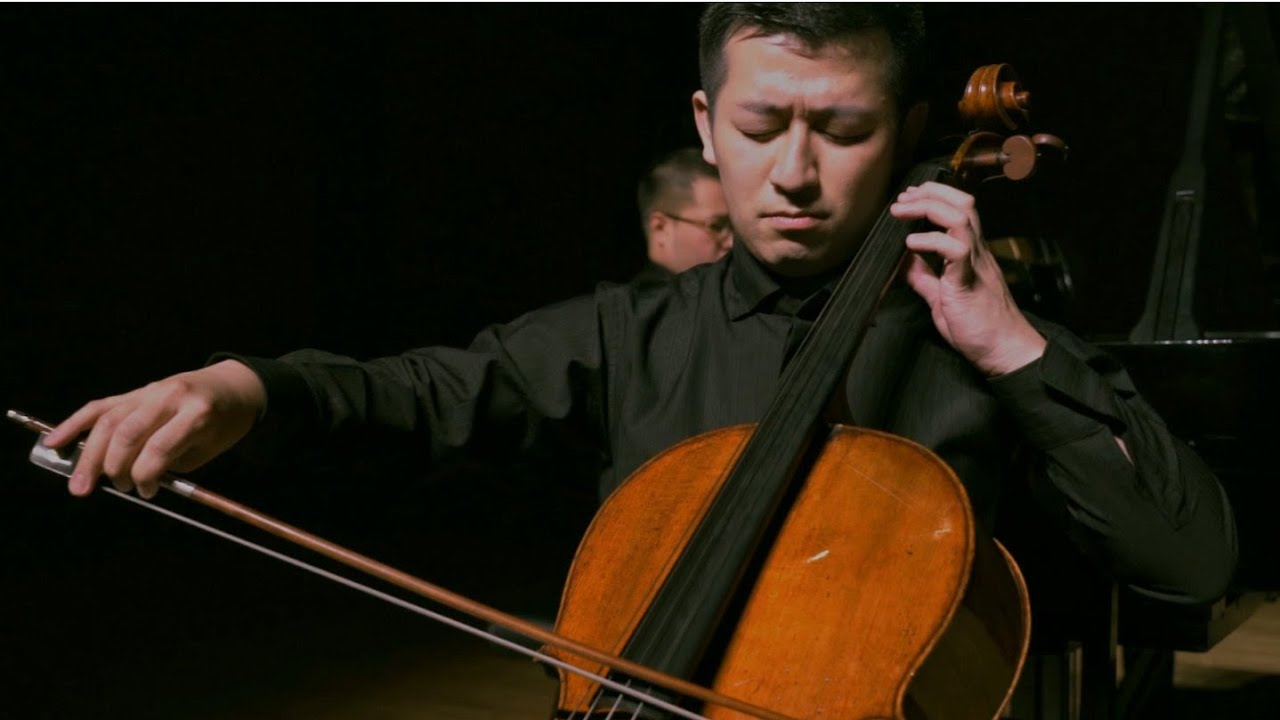
\includegraphics[width=0.48\linewidth]{pictures/youtube/2025/04/20250415_113850_youtube_001_QR50OtY7fhY.jpg}
}
\end{center}

\subsection*{2025年04月16日 08:42}
\addcontentsline{toc}{subsection}{2025年04月16日 08:42}

\paragraph{リンク}
\url{https://youtu.be/uhNUlo_ZJp4}

\begin{center}
\href{https://youtu.be/uhNUlo_ZJp4}{
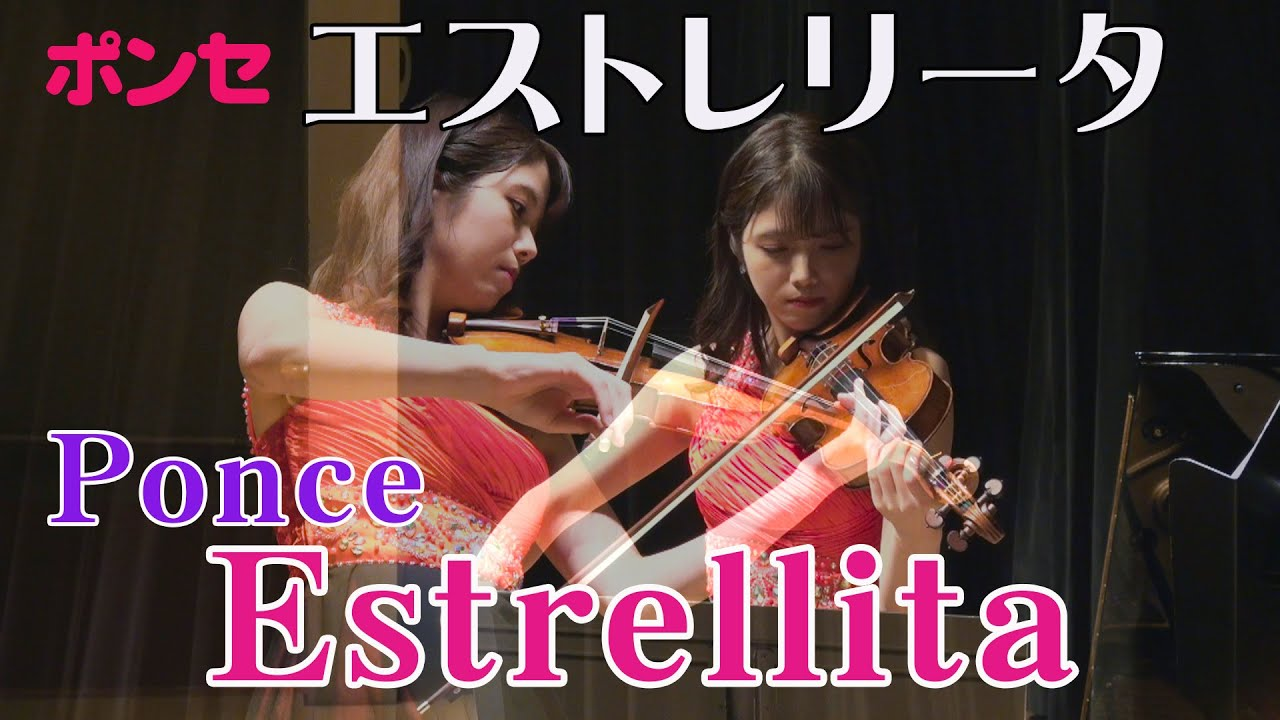
\includegraphics[width=0.48\linewidth]{pictures/youtube/2025/04/20250416_084239_youtube_001_uhNUlo_ZJp4.jpg}
}
\end{center}

\subsection*{2025年04月16日 08:42}
\addcontentsline{toc}{subsection}{2025年04月16日 08:42}

\paragraph{リンク}
\url{https://youtu.be/4gcxlORI25U}

\begin{center}
\href{https://youtu.be/4gcxlORI25U}{
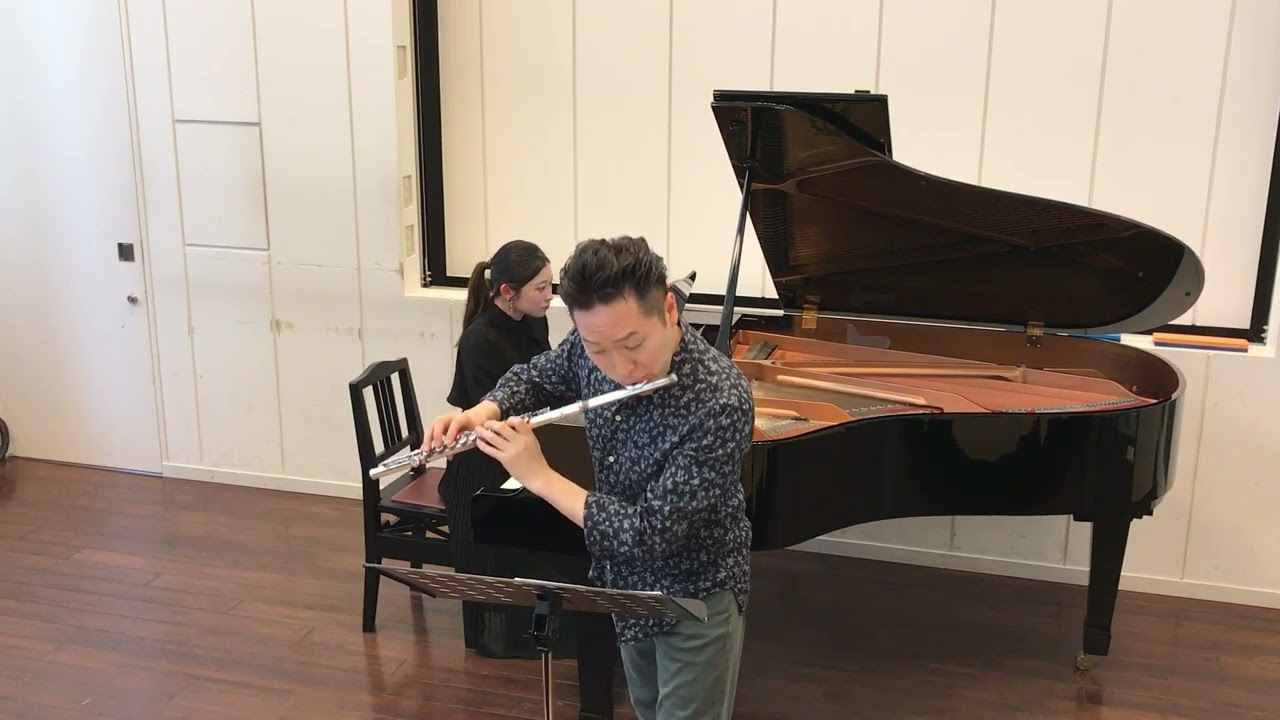
\includegraphics[width=0.48\linewidth]{pictures/youtube/2025/04/20250416_084257_youtube_001_4gcxlORI25U.jpg}
}
\end{center}

\subsection*{2025年04月16日 08:45}
\addcontentsline{toc}{subsection}{2025年04月16日 08:45}

\paragraph{リンク}
\url{https://youtu.be/cKmOpmyQlEY}

\begin{center}
\href{https://youtu.be/cKmOpmyQlEY}{
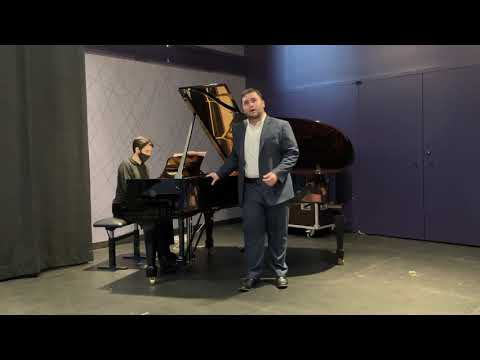
\includegraphics[width=0.48\linewidth]{pictures/youtube/2025/04/20250416_084540_youtube_001_cKmOpmyQlEY.jpg}
}
\end{center}

\subsection*{2025年04月16日 08:47}
\addcontentsline{toc}{subsection}{2025年04月16日 08:47}

\paragraph{リンク}
\url{https://youtu.be/Fnsr-xQryZ0}

\begin{center}
\href{https://youtu.be/Fnsr-xQryZ0}{
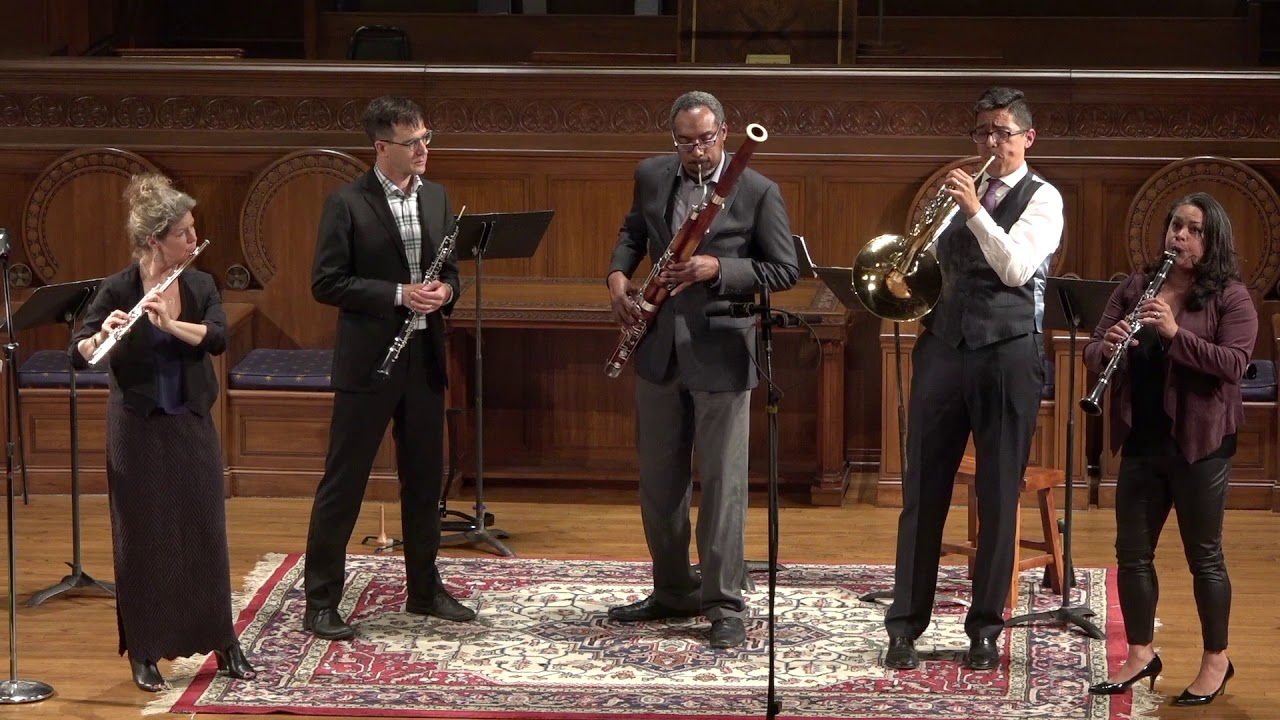
\includegraphics[width=0.48\linewidth]{pictures/youtube/2025/04/20250416_084717_youtube_001_Fnsr-xQryZ0.jpg}
}
\end{center}

\subsection*{2025年04月16日 08:49}
\addcontentsline{toc}{subsection}{2025年04月16日 08:49}

\paragraph{リンク}
\url{https://youtu.be/gyuadW72waM}

\begin{center}
\href{https://youtu.be/gyuadW72waM}{
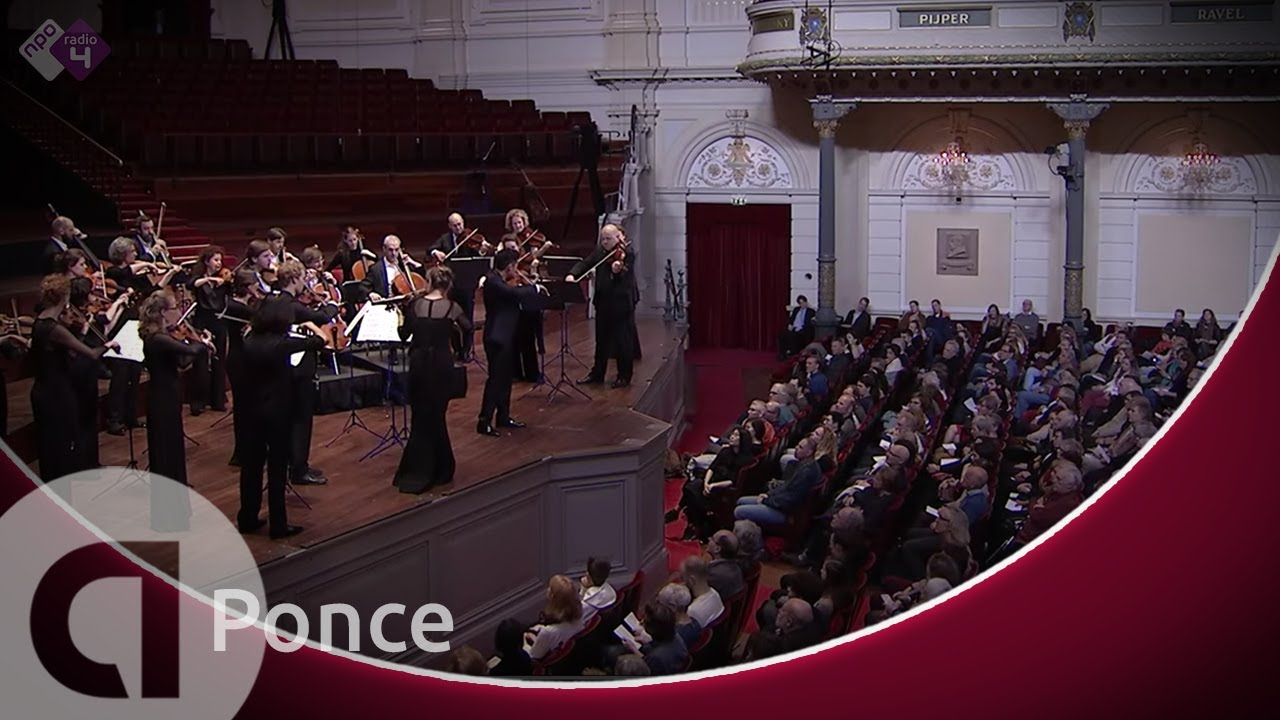
\includegraphics[width=0.48\linewidth]{pictures/youtube/2025/04/20250416_084906_youtube_001_gyuadW72waM.jpg}
}
\end{center}

\subsection*{2025年04月17日 06:10}
\addcontentsline{toc}{subsection}{2025年04月17日 06:10}

\paragraph{リンク}
\url{https://youtu.be/MVWtosCE4J4}

\begin{center}
\href{https://youtu.be/MVWtosCE4J4}{
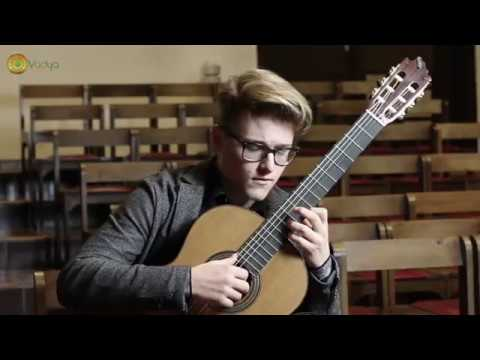
\includegraphics[width=0.48\linewidth]{pictures/youtube/2025/04/20250417_061025_youtube_001_MVWtosCE4J4.jpg}
}
\end{center}

\subsection*{2025年04月20日 21:57}
\addcontentsline{toc}{subsection}{2025年04月20日 21:57}

\url{https://youtu.be/CYFFv1RlMu0}

\begin{center}
\href{https://youtu.be/CYFFv1RlMu0}{
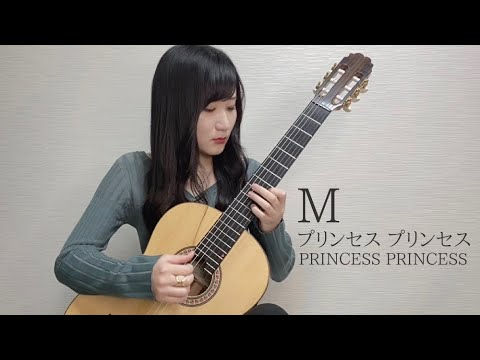
\includegraphics[width=0.48\linewidth]{pictures/youtube/2025/04/20250420_215713_youtube_001_CYFFv1RlMu0.jpg}
}
\end{center}




何を思ったのか？

エストレリータの練習をしていたはずなのですが、いつの間にかよそ見してしまい、何故かこの曲の楽譜をゲットしていました。

\subsection*{2025年04月20日 21:59}
\addcontentsline{toc}{subsection}{2025年04月20日 21:59}

\paragraph{リンク}
\url{https://youtu.be/fDJEtqt_zd8}

\begin{center}
\href{https://youtu.be/fDJEtqt_zd8}{
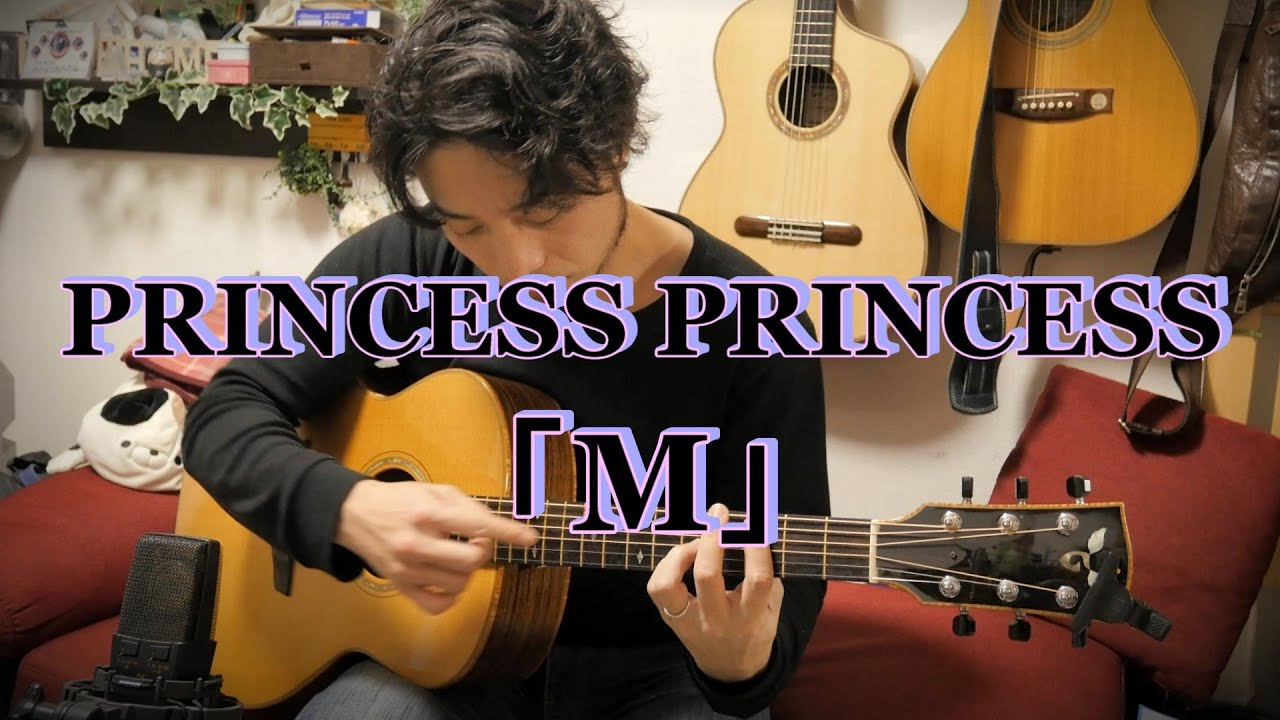
\includegraphics[width=0.48\linewidth]{pictures/youtube/2025/04/20250420_215908_youtube_001_fDJEtqt_zd8.jpg}
}
\end{center}

\subsection*{2025年04月20日 22:29}
\addcontentsline{toc}{subsection}{2025年04月20日 22:29}

\paragraph{リンク}
\url{https://youtu.be/VkCelHGk550}

\begin{center}
\href{https://youtu.be/VkCelHGk550}{
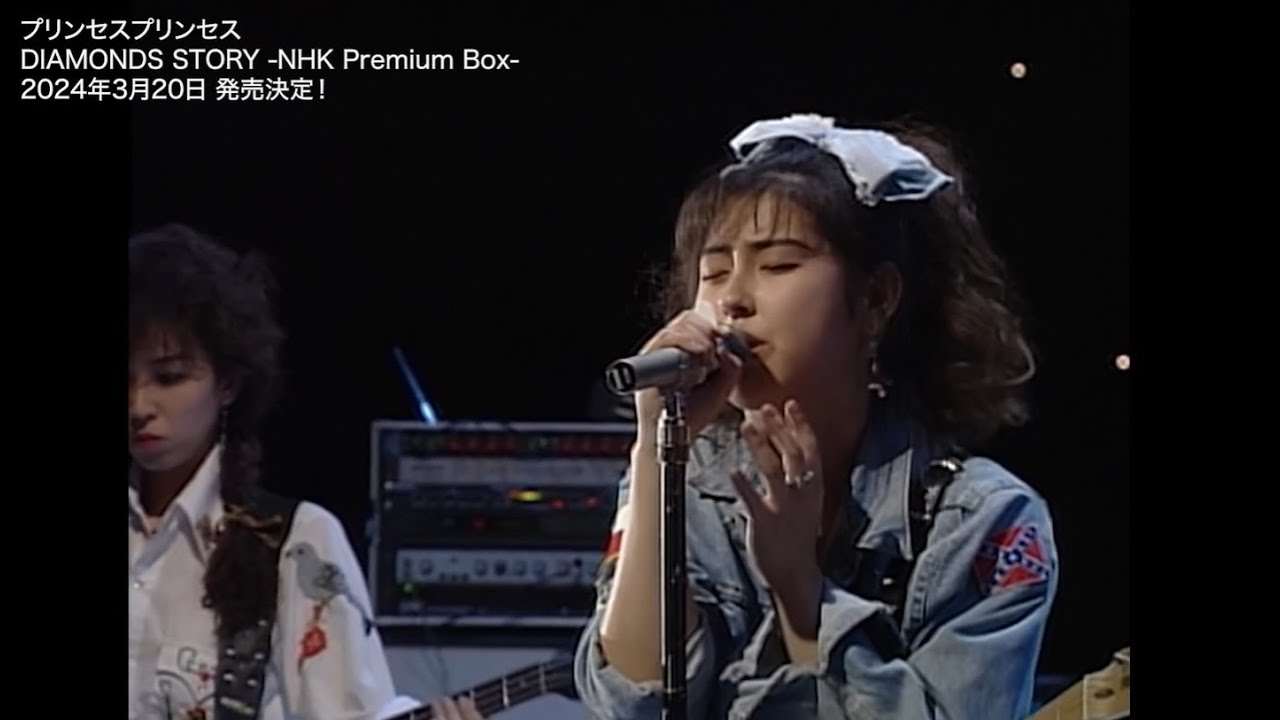
\includegraphics[width=0.48\linewidth]{pictures/youtube/2025/04/20250420_222932_youtube_001_VkCelHGk550.jpg}
}
\end{center}

\subsection*{2025年04月21日 01:33}
\addcontentsline{toc}{subsection}{2025年04月21日 01:33}

\paragraph{リンク}
\url{https://youtu.be/lt3iHD1EKZM}

\begin{center}
\href{https://youtu.be/lt3iHD1EKZM}{
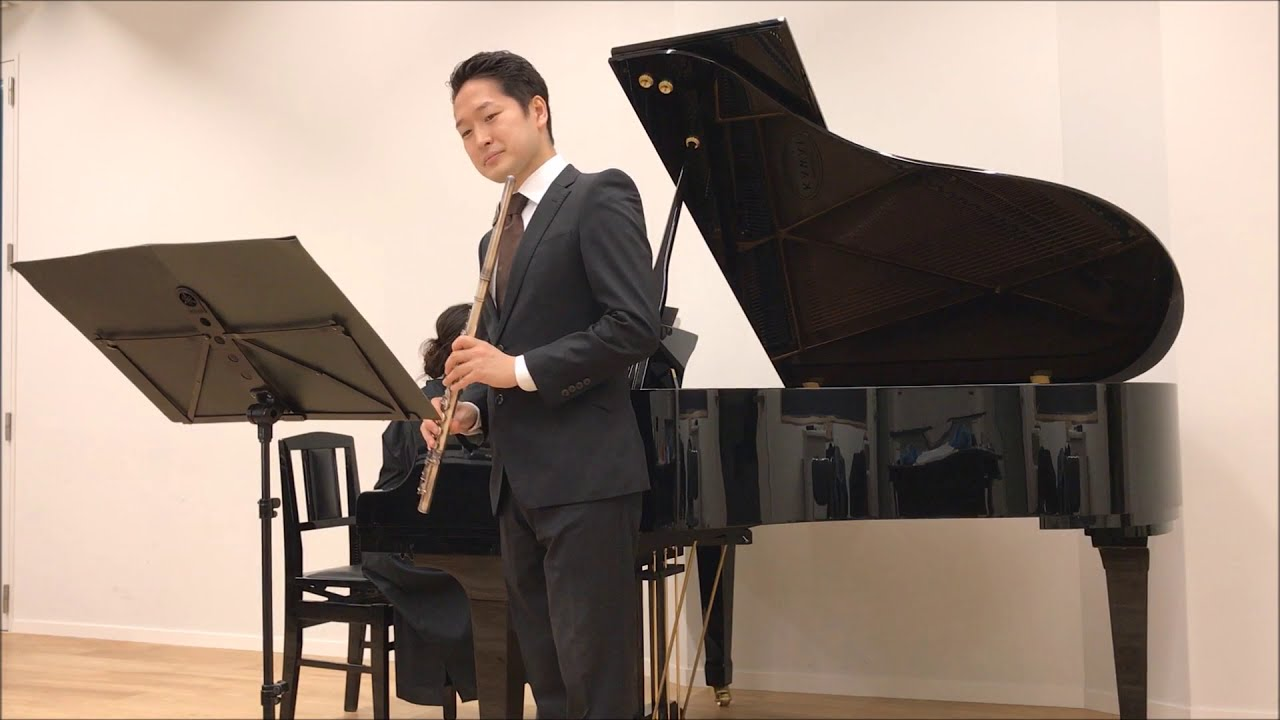
\includegraphics[width=0.48\linewidth]{pictures/youtube/2025/04/20250421_013325_youtube_001_lt3iHD1EKZM.jpg}
}
\end{center}

\subsection*{2025年04月21日 03:50}
\addcontentsline{toc}{subsection}{2025年04月21日 03:50}

\paragraph{リンク}
\url{https://youtu.be/A0WF7RSflq8}

\begin{center}
\href{https://youtu.be/A0WF7RSflq8}{
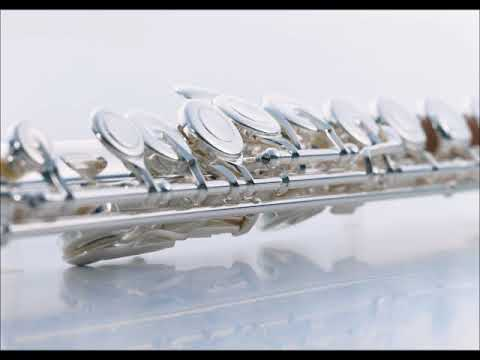
\includegraphics[width=0.48\linewidth]{pictures/youtube/2025/04/20250421_035021_youtube_001_A0WF7RSflq8.jpg}
}
\end{center}

\subsection*{2025年04月22日 09:33}
\addcontentsline{toc}{subsection}{2025年04月22日 09:33}

\#PyCharm で（不意に）現れてきていた \#Python の \#AIアシスタント （ \#JetBrains ）でしたが、どうも30日間の試用期間が終了したみたいです。AI Free から AI Pro へ移行せよとのことらしいのだが、Yearlyでの契約なら1166.67円/月、Monthlyでの契約なら1400円/月という事の様だ。(1400-1166.67)x12=2799.96円


とても便利だったのに、話し相手がいなくなったみたいで、ちょっと寂しい。

\paragraph{写真}
\begin{center}
\begin{minipage}{0.48\linewidth}
\centering
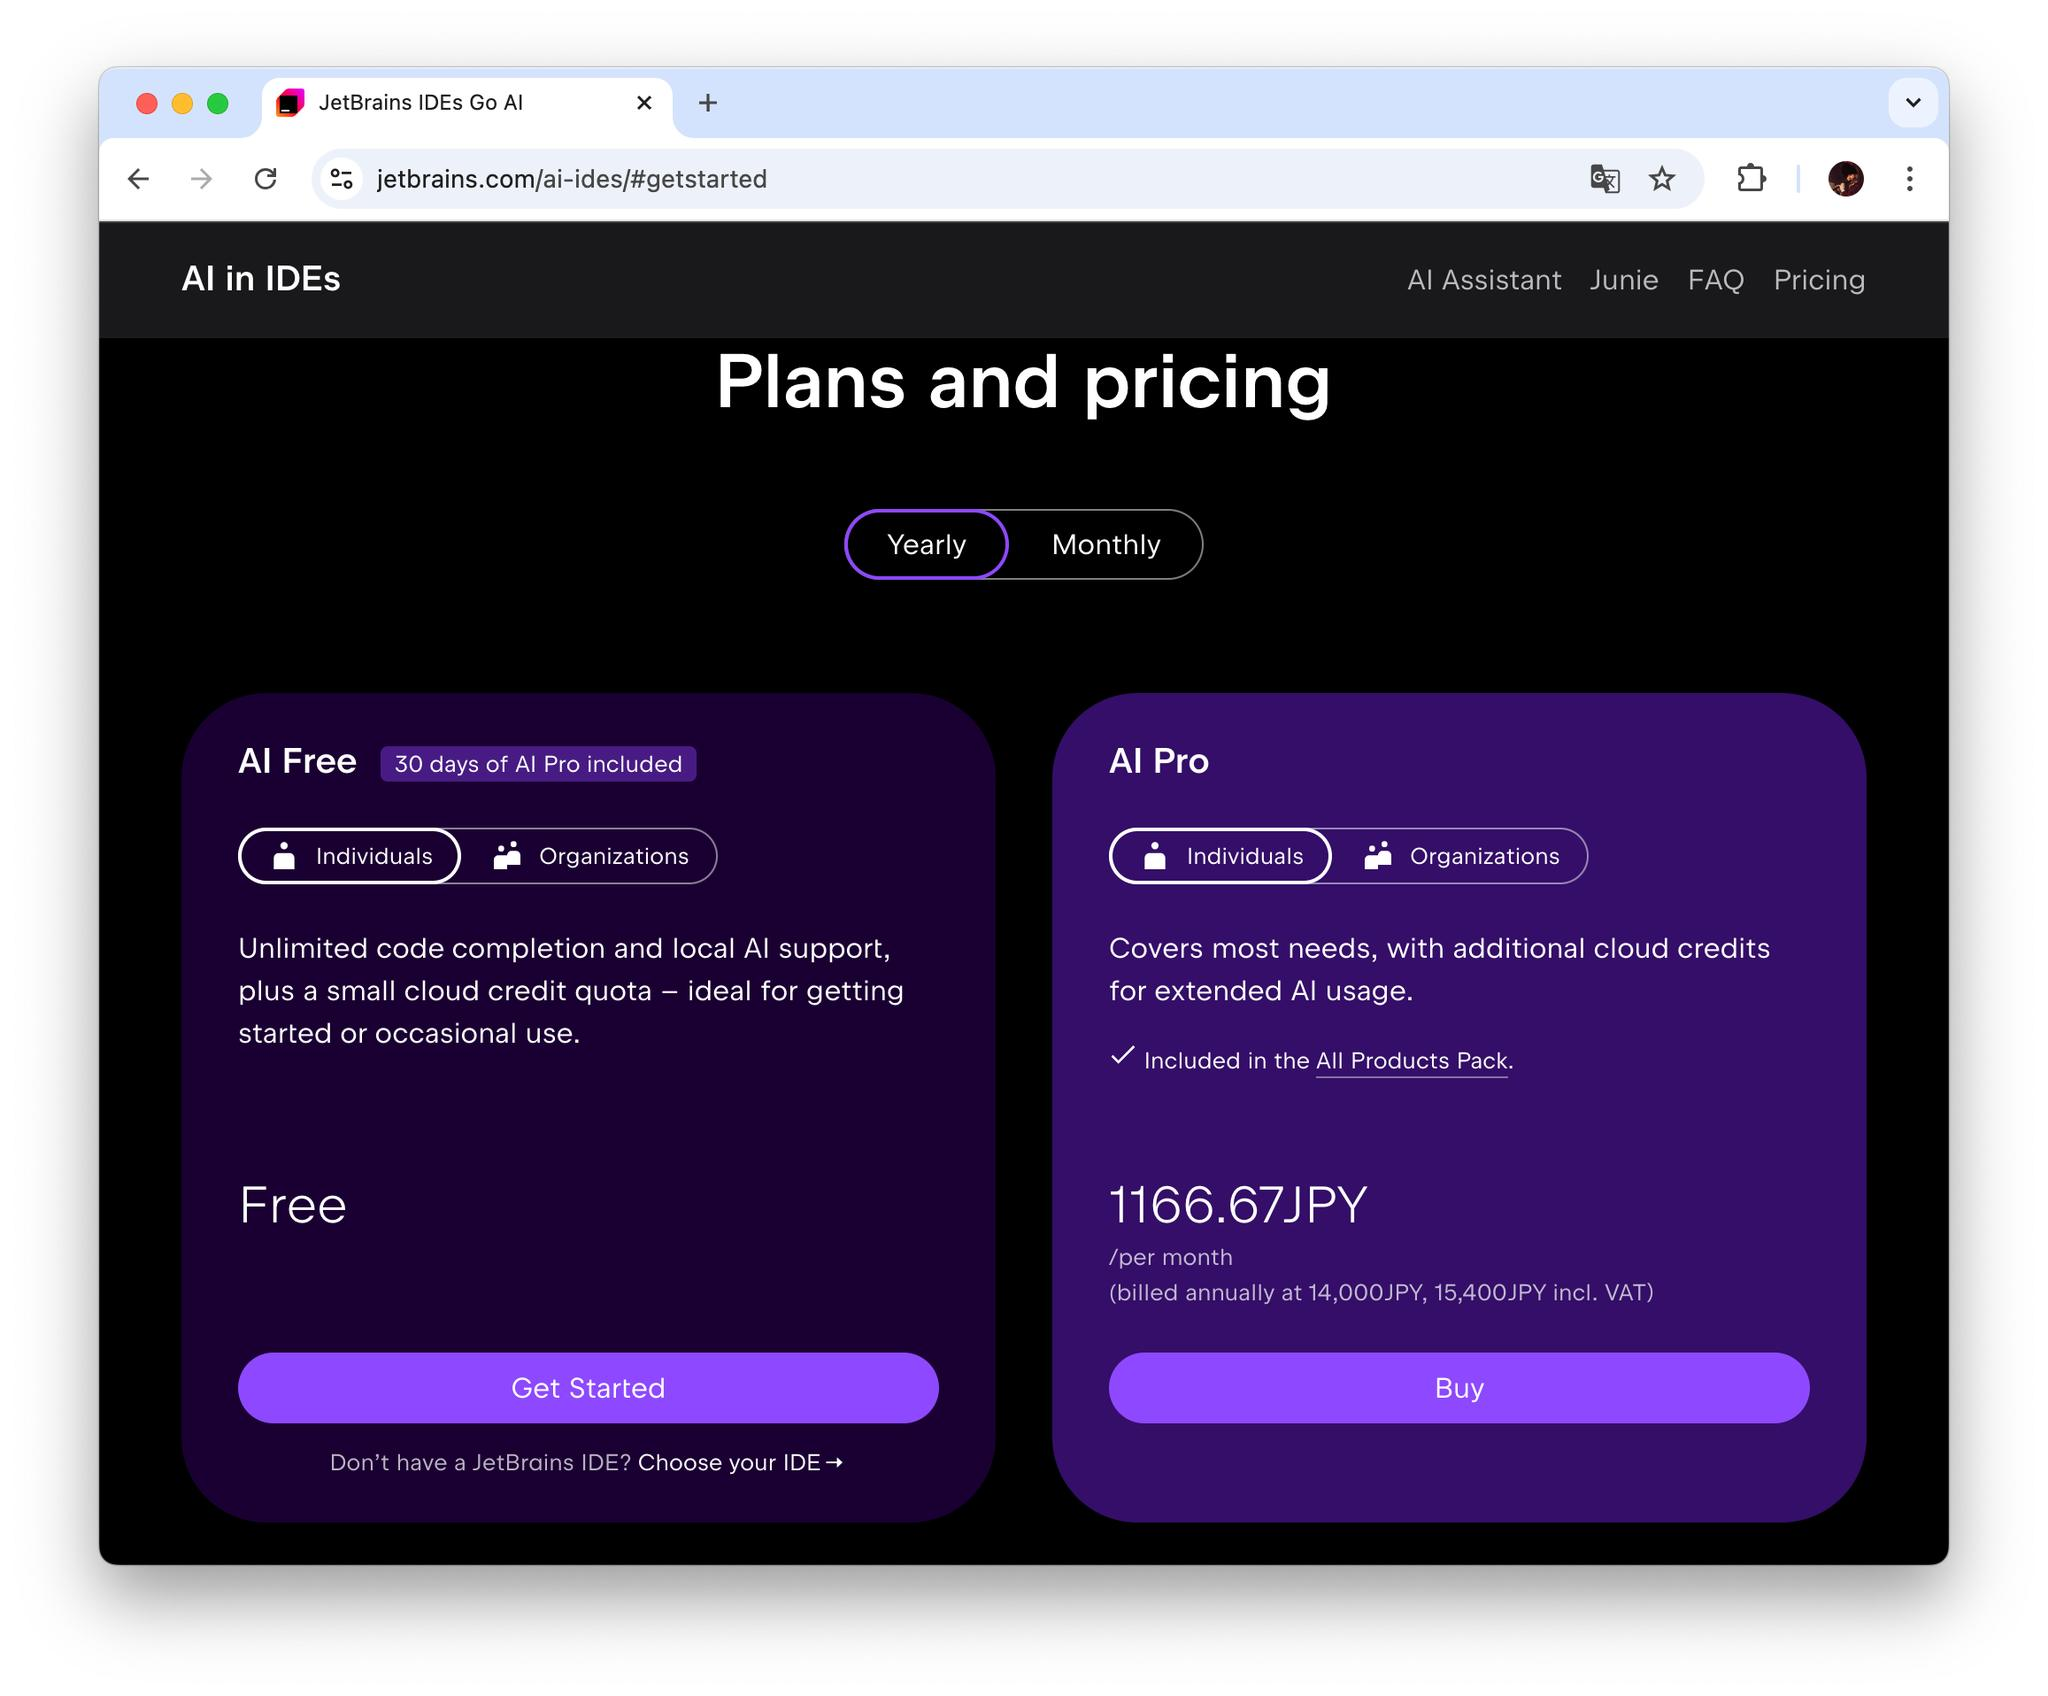
\includegraphics[width=\linewidth]{pictures/2025/04/20250422_093357_001.jpg}
\end{minipage}
\end{center}

\subsection*{2025年04月22日 13:17}
\addcontentsline{toc}{subsection}{2025年04月22日 13:17}

\url{https://github.com/smat1957/QA4U/tree/main/TravelingSalesman}




\#巡回セールスマン問題 もまた、最適化関連の分野では古典中の古典なので、\#量子コンピュータ で一度はクリアしておかなければと思い、考えはじめた。


セールスマンは「同時に複数の街に訪れることはない」「どの街にも一回しか訪れない」。この二つの制約を \#QUBO に落とし込むのは容易だ。ところが、\#目的関数 「セールスマンが巡った距離の総和を最小に」で、どうやってQUBOに落とし込めばいいのか、はたと困ってしまった。「街を取っ替え引っ替え」して、さらに「時刻も取っ替え引っ替え」するとして、結局「QUBOの何処」を書き換えたらいいのか？そもそも \#決定変数 ですが、「その街i をその時刻tに訪れるか否か」ではなくて、「時刻tにiの街からjの街へ移動するか否か」にしたらどうなるのか？「i の街からj の街への移動」とその逆方向の移動とは別に考えなくてもいいのか？最後に訪れた街から、スタートした街に戻る距離も目的函数の計算に含めなきゃいけないのではないか？街と街の間の全ての組み合わせについて、その全てに予めコストが与えられているとは限らないでしょう。


などなど、と考え倦ねていると、こんな（↓下のリンク）記事があった。街の数が4つの場合のQUBO行列の中の様子が具体的に示されていて、感心する事しきりです。

便利な時代になったものだ。つくづく思います。昔だったら、こんな所で考え倦ねることになったら、完全に立ち止まってしまって、一歩も先に進めなくなっていたと思います。（心配？しなくても、今も昔も「誰か考えてくれてる人がいる」事だけは確かだ）


という事で、巡回セールスマン問題をいつもの \#Openjij の \#SASampler で解けましたら、その \#Python ソースやPDFドキュメント、\#TeX ソース等一式を、例の \#GitHub に置いておこうと思います。（↑冒頭のリンク）


参考にした情報：

\url{https://qiita.com/yabish/items/9f42e3752174aef8b79f}



\paragraph{写真}
\begin{center}
\begin{minipage}{0.48\linewidth}
\centering
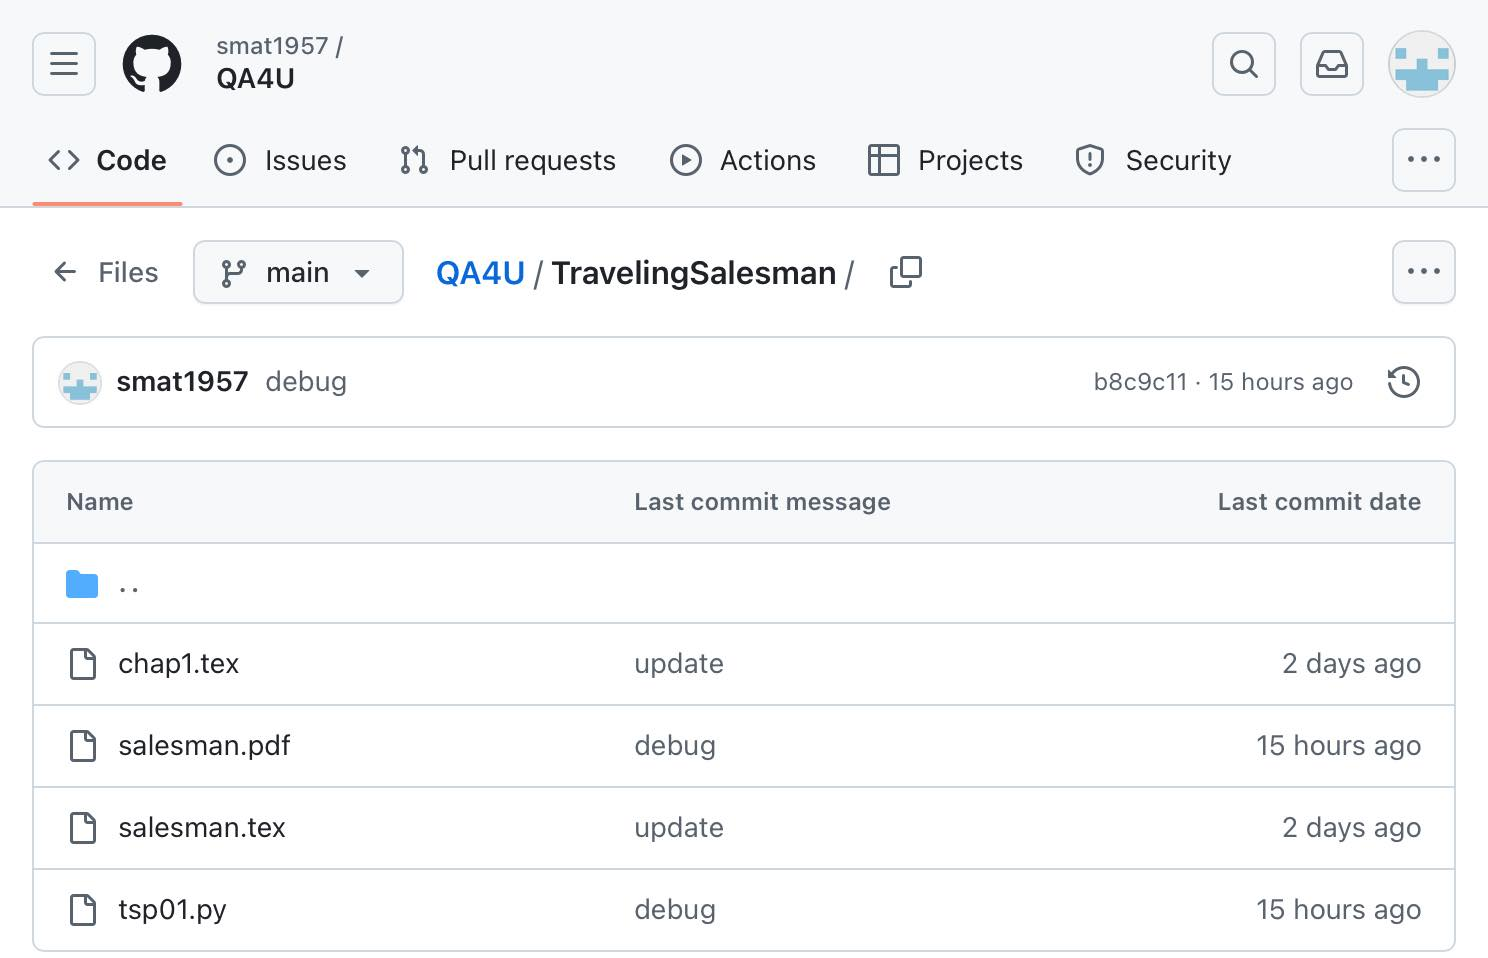
\includegraphics[width=\linewidth]{pictures/2025/04/20250422_131741_001.jpg}
\end{minipage}
\end{center}

\subsection*{2025年04月23日 23:24}
\addcontentsline{toc}{subsection}{2025年04月23日 23:24}

\paragraph{リンク}
\url{https://youtu.be/pejqM7tIJBs}

\begin{center}
\href{https://youtu.be/pejqM7tIJBs}{
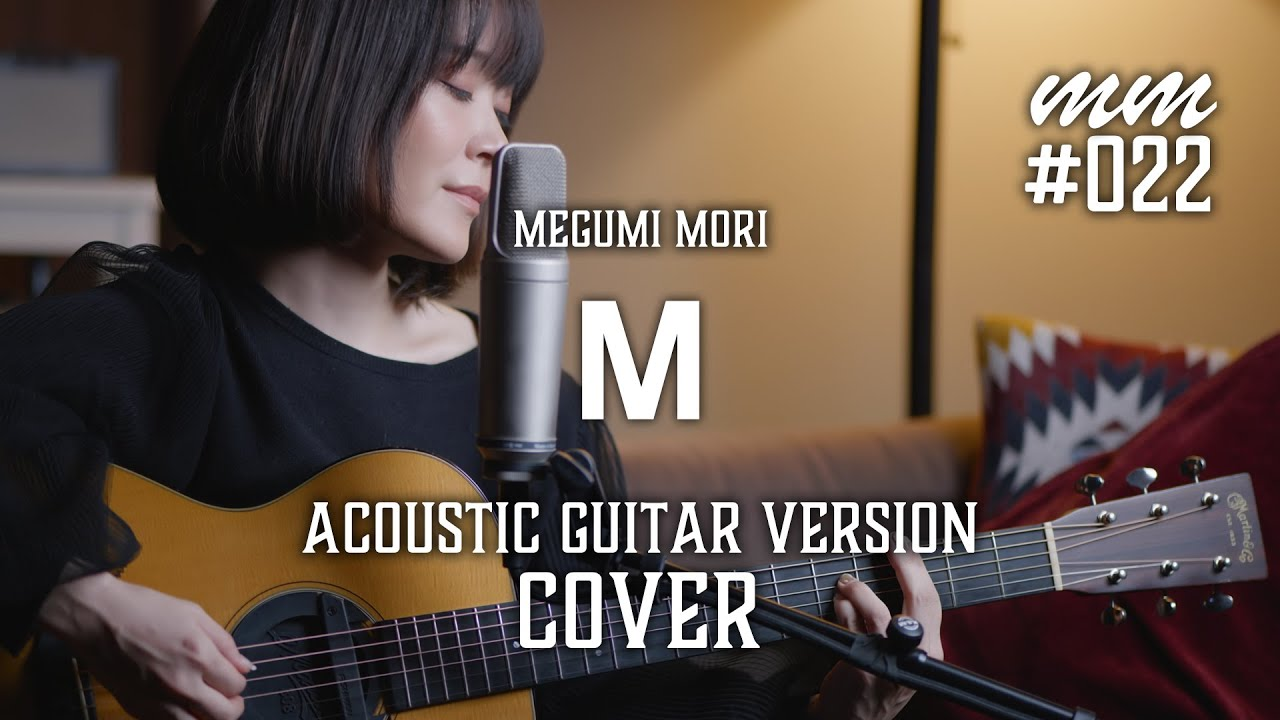
\includegraphics[width=0.48\linewidth]{pictures/youtube/2025/04/20250423_232436_youtube_001_pejqM7tIJBs.jpg}
}
\end{center}

\subsection*{2025年04月25日 09:17}
\addcontentsline{toc}{subsection}{2025年04月25日 09:17}

\url{https://github.com/smat1957/QA4U/tree/main/MagicCircle}




\#魔方陣 を \#量子コンピュータ （ \#Openjij の \#SASampler ）で解く \#Python のプログラム。自分に分かる内容にして（言語化？）整理してみた。いつもの通り \#TeX のドキュメントと一緒に、 \#GitHub に置いておくことにします。


出力される「結果をチェックして、ふるい（分け）にかける仕組み」を追加する必要がありましたね。


（その後）

「結果をチェックする、ふるい（分け）する仕組み」を追加、更新しました。num\_reads=1000くらいで、チェックをパスできた解が出力される様になります。また、対称なものもチェックで除外できればよかったんだけど、ここまでで妥協する事にしました。

\paragraph{写真}
\begin{center}
\begin{minipage}{0.48\linewidth}
\centering
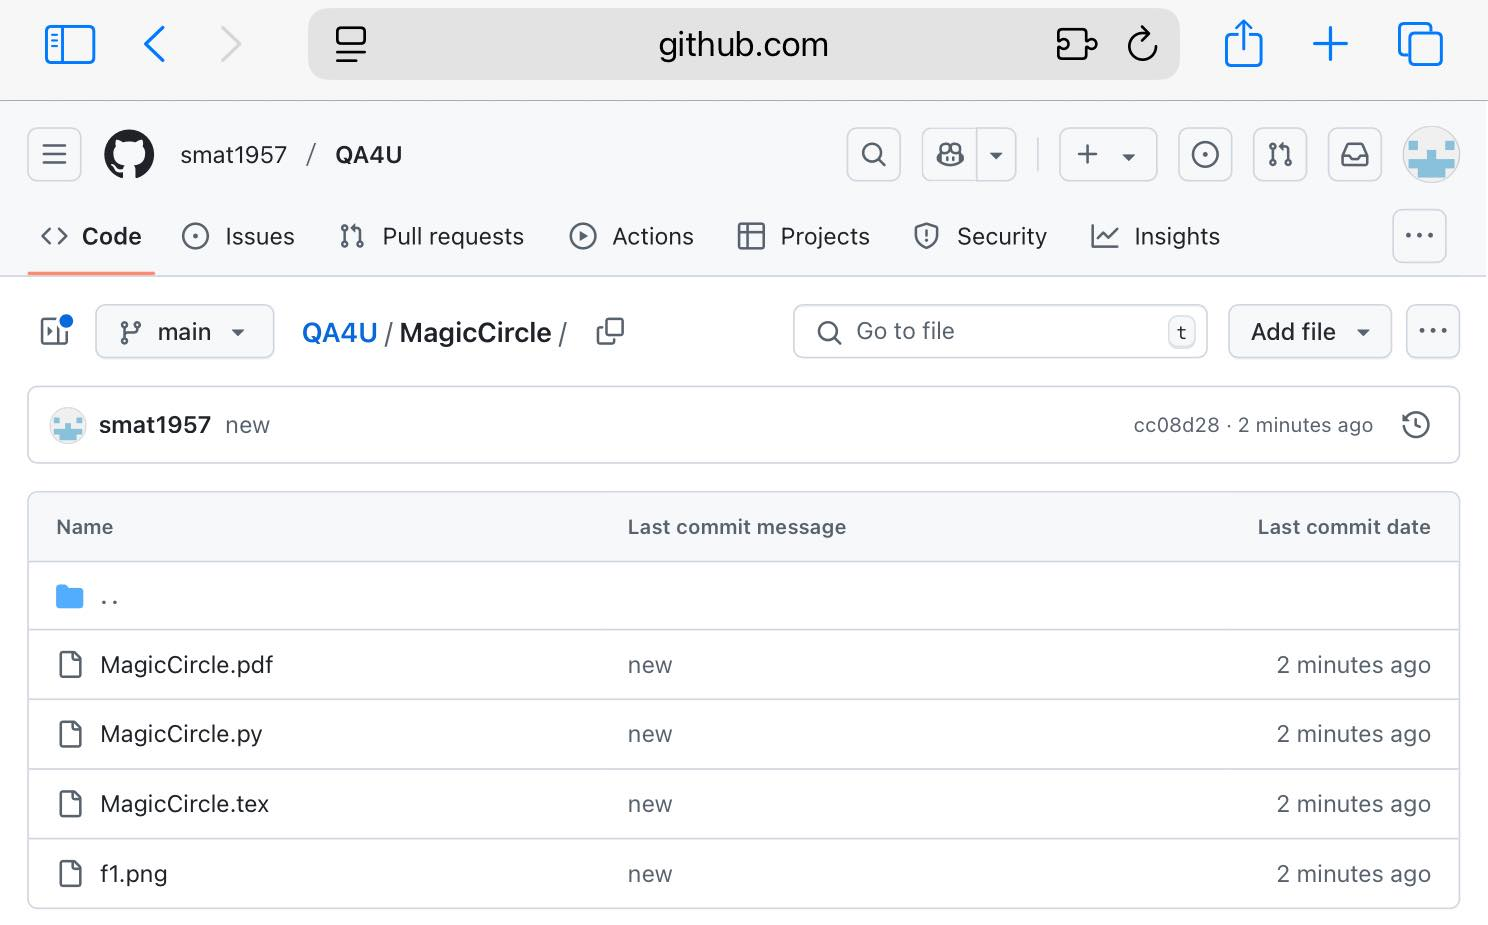
\includegraphics[width=\linewidth]{pictures/2025/04/20250425_091751_001.jpg}
\end{minipage}
\end{center}

\subsection*{2025年04月26日 05:51}
\addcontentsline{toc}{subsection}{2025年04月26日 05:51}

\paragraph{リンク}
\url{https://youtu.be/UV2UEgaQLbY}

\begin{center}
\href{https://youtu.be/UV2UEgaQLbY}{
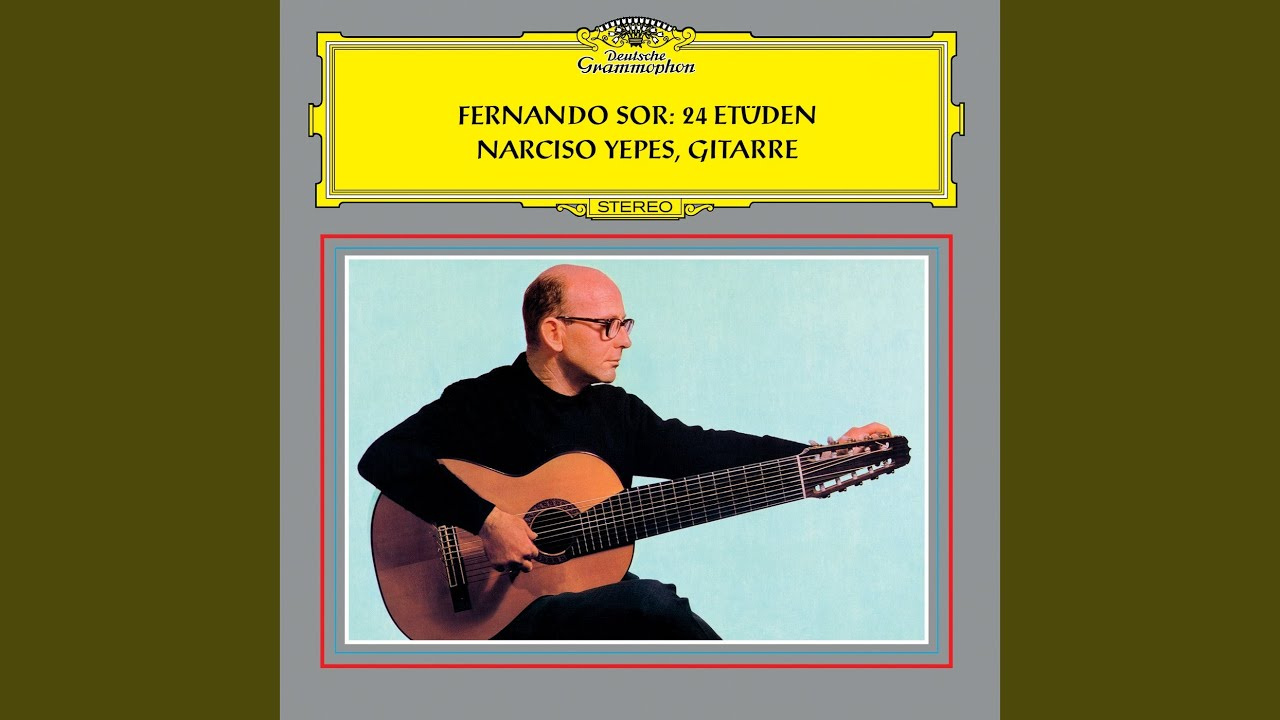
\includegraphics[width=0.48\linewidth]{pictures/youtube/2025/04/20250426_055150_youtube_001_UV2UEgaQLbY.jpg}
}
\end{center}

\subsection*{2025年04月26日 05:58}
\addcontentsline{toc}{subsection}{2025年04月26日 05:58}

\paragraph{リンク}
\url{https://youtu.be/v9jRbYIA6lw}

\begin{center}
\href{https://youtu.be/v9jRbYIA6lw}{
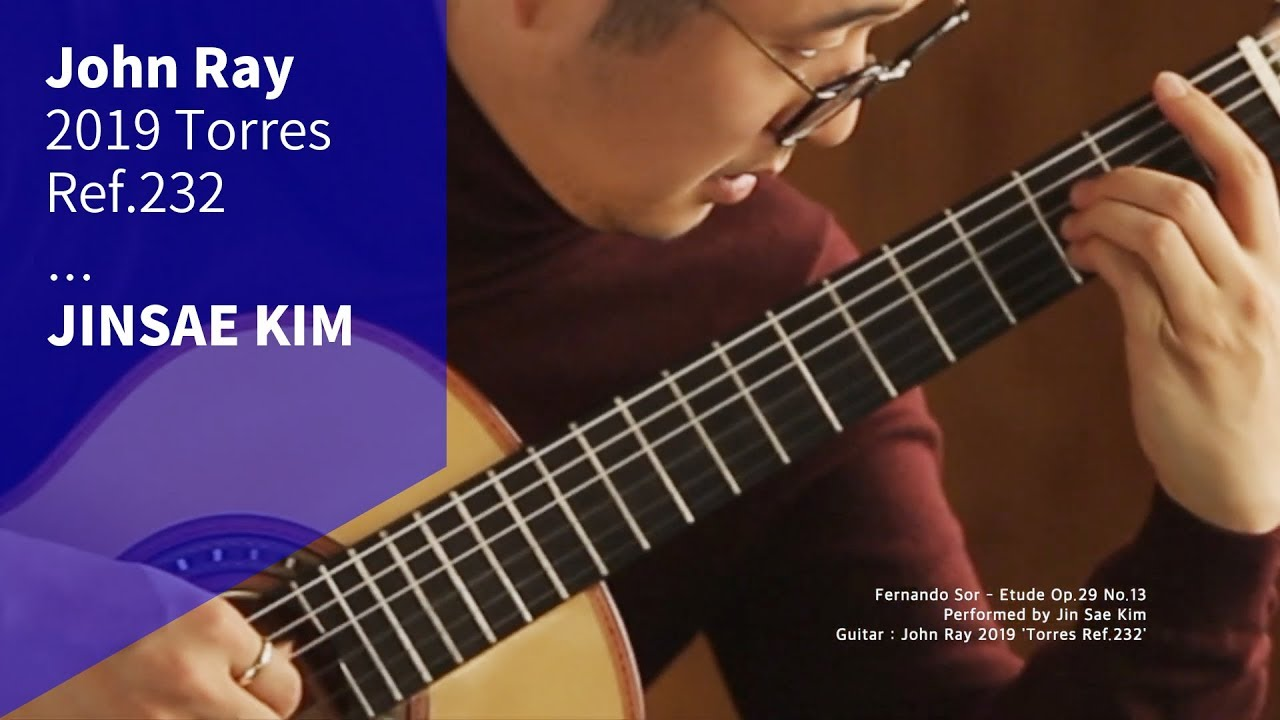
\includegraphics[width=0.48\linewidth]{pictures/youtube/2025/04/20250426_055842_youtube_001_v9jRbYIA6lw.jpg}
}
\end{center}

\subsection*{2025年04月26日 06:01}
\addcontentsline{toc}{subsection}{2025年04月26日 06:01}

\paragraph{リンク}
\url{https://youtu.be/ztQEhAL3-Fk}

\begin{center}
\href{https://youtu.be/ztQEhAL3-Fk}{
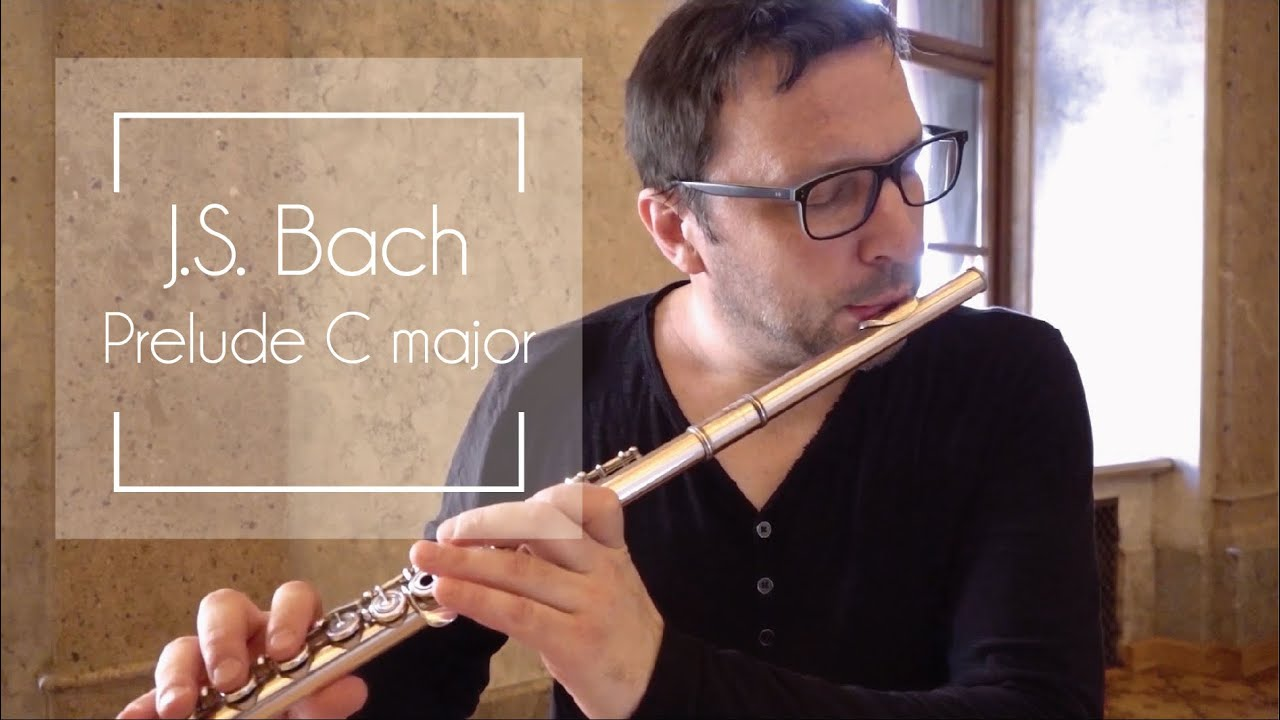
\includegraphics[width=0.48\linewidth]{pictures/youtube/2025/04/20250426_060126_youtube_001_ztQEhAL3-Fk.jpg}
}
\end{center}

\subsection*{2025年04月26日 13:55}
\addcontentsline{toc}{subsection}{2025年04月26日 13:55}

\url{https://youtu.be/uOuDzjCHeM4}

\begin{center}
\href{https://youtu.be/uOuDzjCHeM4}{
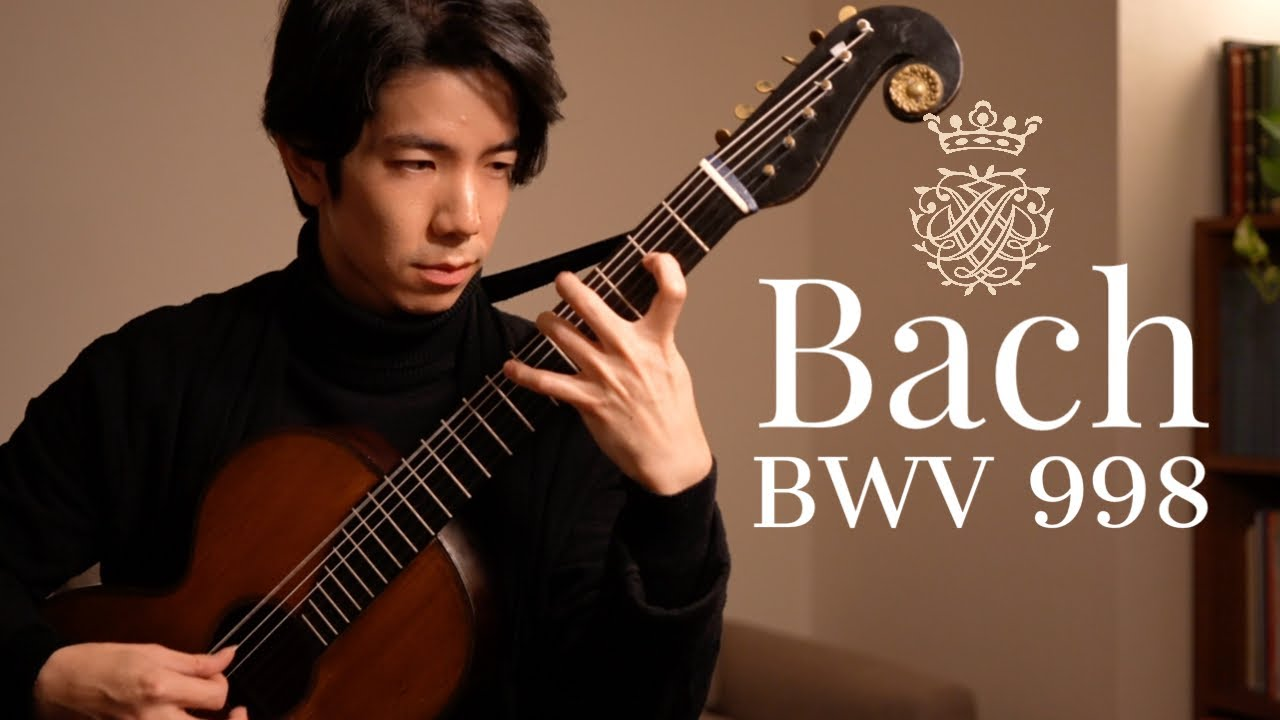
\includegraphics[width=0.48\linewidth]{pictures/youtube/2025/04/20250426_135506_youtube_001_uOuDzjCHeM4.jpg}
}
\end{center}




19世紀ギターの音が魅力的です。

落ち着いた、しかし熱量も感じられる素敵な演奏、好きな演奏です。

\subsection*{2025年04月27日 11:43}
\addcontentsline{toc}{subsection}{2025年04月27日 11:43}

\url{https://github.com/smat1957/QA4U/tree/main/NumberPlace}




今度は \#数独 をこれまでと同じ様な調子で (\#量子コンピュータ で)解こうとしている。

昨日から（J.S.BachをBGMに聴きながら）あれやこれや苦戦しているのですが、現段階で満足できる状態ではない。何度も試行していると、正解が出る「こともある」のだが、これで解けたと言っていいのか？もっとヒット率を上げられないのか。

9x9の数独。1\textasciitilde{}9が行にも列にもブロックにも重複無く収まった状態というものはすぐに（幾つでも）出来てくる。ところが、予め決まっているセルの数値を固定しようとすると解に至らない。4x4なら解ける。9x9が解けない。難易度によるのかもしれない。（新聞連載の一つ星の問題から試してみるかな）


数独を解くのに、何か（忘れている）決定的な制約条件でもある？

「解けない自分と同じレベル」のプログラムになっている＝解けない自分のレベルでしか制約条件を設定できていないという事、なのかもしれない。


プログラム等はいつもの \#GitHub に置きましたが、スッキリしない、、、

\paragraph{写真}
\begin{center}
\begin{minipage}{0.48\linewidth}
\centering
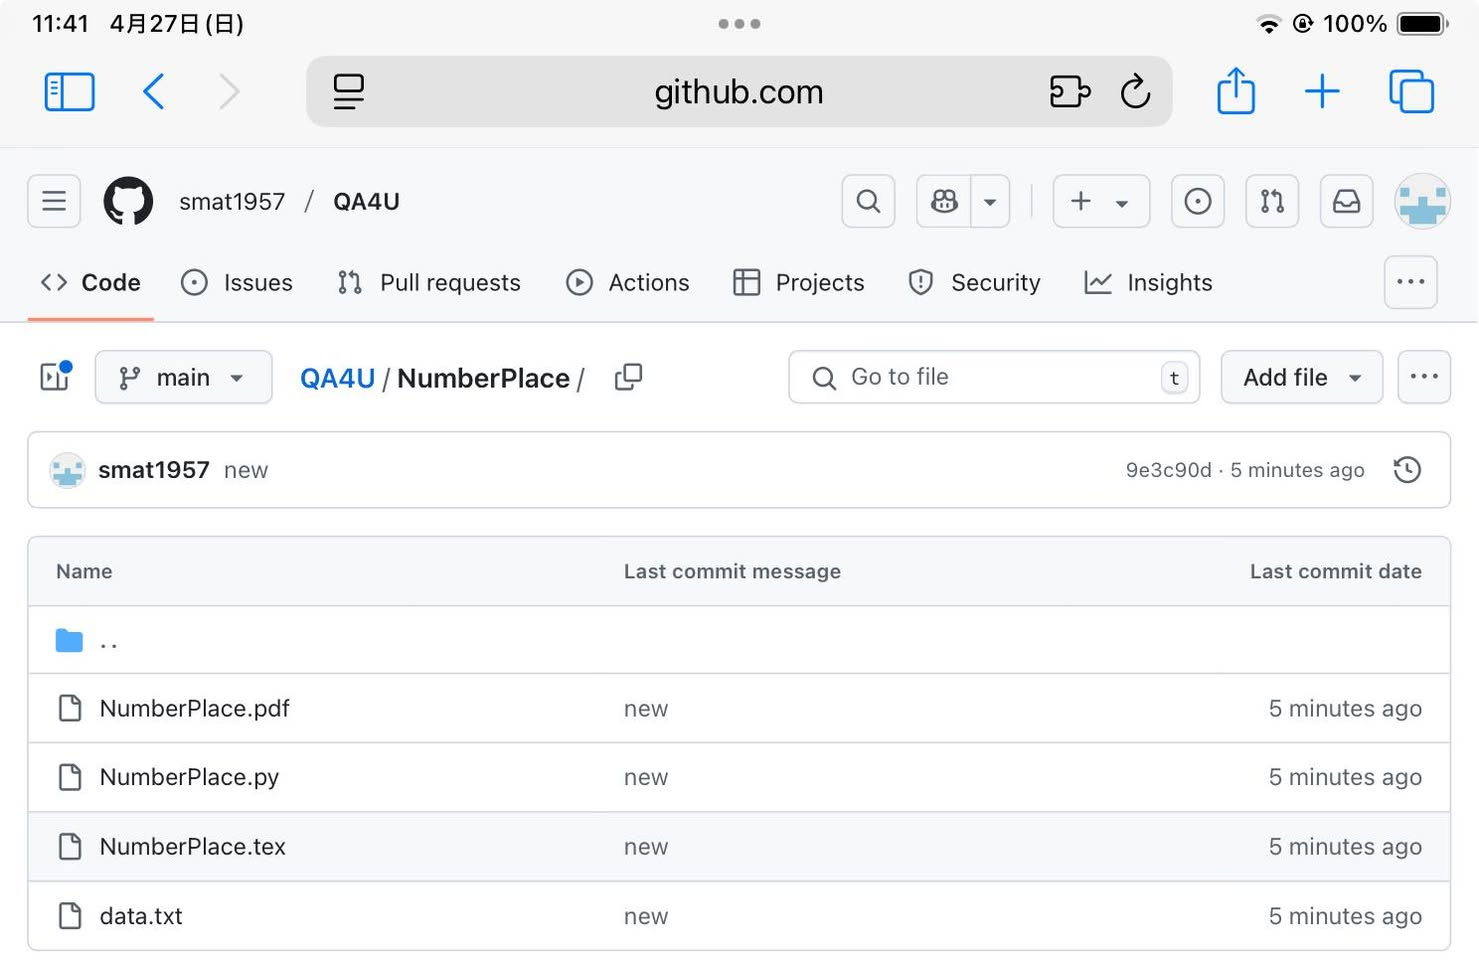
\includegraphics[width=\linewidth]{pictures/2025/04/20250427_114321_001.jpg}
\end{minipage}
\end{center}

\section{5月}

\subsection*{2025年05月01日 08:57}
\addcontentsline{toc}{subsection}{2025年05月01日 08:57}

\#量子コンピュータ に \#数独 を解かせることが出来ました！定式化とQUBO生成のプログラムは間違っていなかったんだな。でも、かなり苦戦しました。なんと言っても、各制約の強さを与えるパラメータの組み合わせがデリケートです。（ある程度は「こうやって決めたらいいんじゃないか」というのを経験的に見つけました。が、これがいつも通用するかと言えば心もとない。）

（プログラムとドキュメント類は次の \#GitHub に置きました）

\url{https://github.com/smat1957/QA4U/tree/main/NumberPlace}




量子コンピュータが吐き出す解は、自分ではチェックしていないけれども、\#Python のプログラムで次の一通りの確認をしている。

（１）各セルの数値は1〜9の中の一つである

(２) 各行、各列、各ブロック内の数値に重複はない

(３) 予め数値の与えられているセルがある

この三つのチェックをクリアできたものだけを表示出力するという「ふるい」にかけているので、大丈夫なんじゃないかな。


\#朝日新聞 の記事（

\url{https://info.asahi.com/choiyomi/sudoku/}

）では、「AIに数独の問題を作らせる事も可能だろうけど、難しい問題と、解いていて面白い問題とは別の話」、従って「問題は手作りしている」と話されている。なるほど。いい話だ。


私の様にプログラムで数独を解いて喜んでいるというのも、数独の楽しみ方の一つでしょうね。不思議なもので、五つ星の問題が解けて、その解が出力されると（自分が手で解いたわけでもないのに）やった！という気になります。


朝日新聞：2025.4.29

難易度★☆☆☆☆

0: \_ 6 \_ 5 \_ \_ \_ 4 \_

1: 4 \_ \_ \_ 9 \_ 8 \_ \_

2: 3 \_ 1 \_ \_ 6 \_ 5 \_

3: \_ 3 \_ 7 \_ \_ \_ \_ 8

4: \_ \_ 6 \_ \_ \_ 9 \_ \_

5: 5 \_ \_ \_ \_ 4 \_ 1 \_

6: \_ 2 \_ 4 \_ \_ 7 \_ 3

7: \_ \_ 9 \_ 3 \_ \_ \_ 1

8: \_ 8 \_ \_ \_ 1 \_ 2 \_


[量子コンピュータの解]


[[9 6 8 5 2 3 1 4 7]

[4 5 2 1 9 7 8 3 6]

[3 7 1 8 4 6 2 5 9]

[2 3 4 7 1 9 5 6 8]

[8 1 6 3 5 2 9 7 4]

[5 9 7 6 8 4 3 1 2]

[1 2 5 4 6 8 7 9 3]

[7 4 9 2 3 5 6 8 1]

[6 8 3 9 7 1 4 2 5]]


/*************************/

朝日新聞：2025.4.10

難易度★★★★★

0: 3 \_ \_ \_ 4 \_ 5 \_ \_

1: \_ \_ 1 6 \_ \_ \_ 7 \_

2: \_ 6 \_ \_ \_ \_ \_ \_ 2

3: \_ \_ \_ 9 \_ \_ 3 \_ \_

4: 7 \_ \_ \_ 5 \_ \_ \_ 4

5: \_ \_ 8 \_ \_ 1 \_ \_ \_

6: 4 \_ \_ \_ \_ \_ \_ 1 \_

7: \_ 3 \_ \_ \_ 6 8 \_ \_

8: \_ \_ 2 \_ 7 \_ \_ \_ 9


[量子コンピュータの解]


[[3 2 7 1 4 8 5 9 6]

[9 5 1 6 2 3 4 7 8]

[8 6 4 7 9 5 1 3 2]

[2 4 5 9 6 7 3 8 1]

[7 1 3 8 5 2 9 6 4]

[6 9 8 4 3 1 7 2 5]

[4 7 6 5 8 9 2 1 3]

[5 3 9 2 1 6 8 4 7]

[1 8 2 3 7 4 6 5 9]]


===

これは以下の記事の続きです

\url{https://m.facebook.com/story.php?story_fbid=9589288864488522&id=100002225117991}




（その後）

朝日新聞の記事はリンク切れ(404)になっていました

\paragraph{写真}
\begin{center}
\begin{minipage}{0.48\linewidth}
\centering
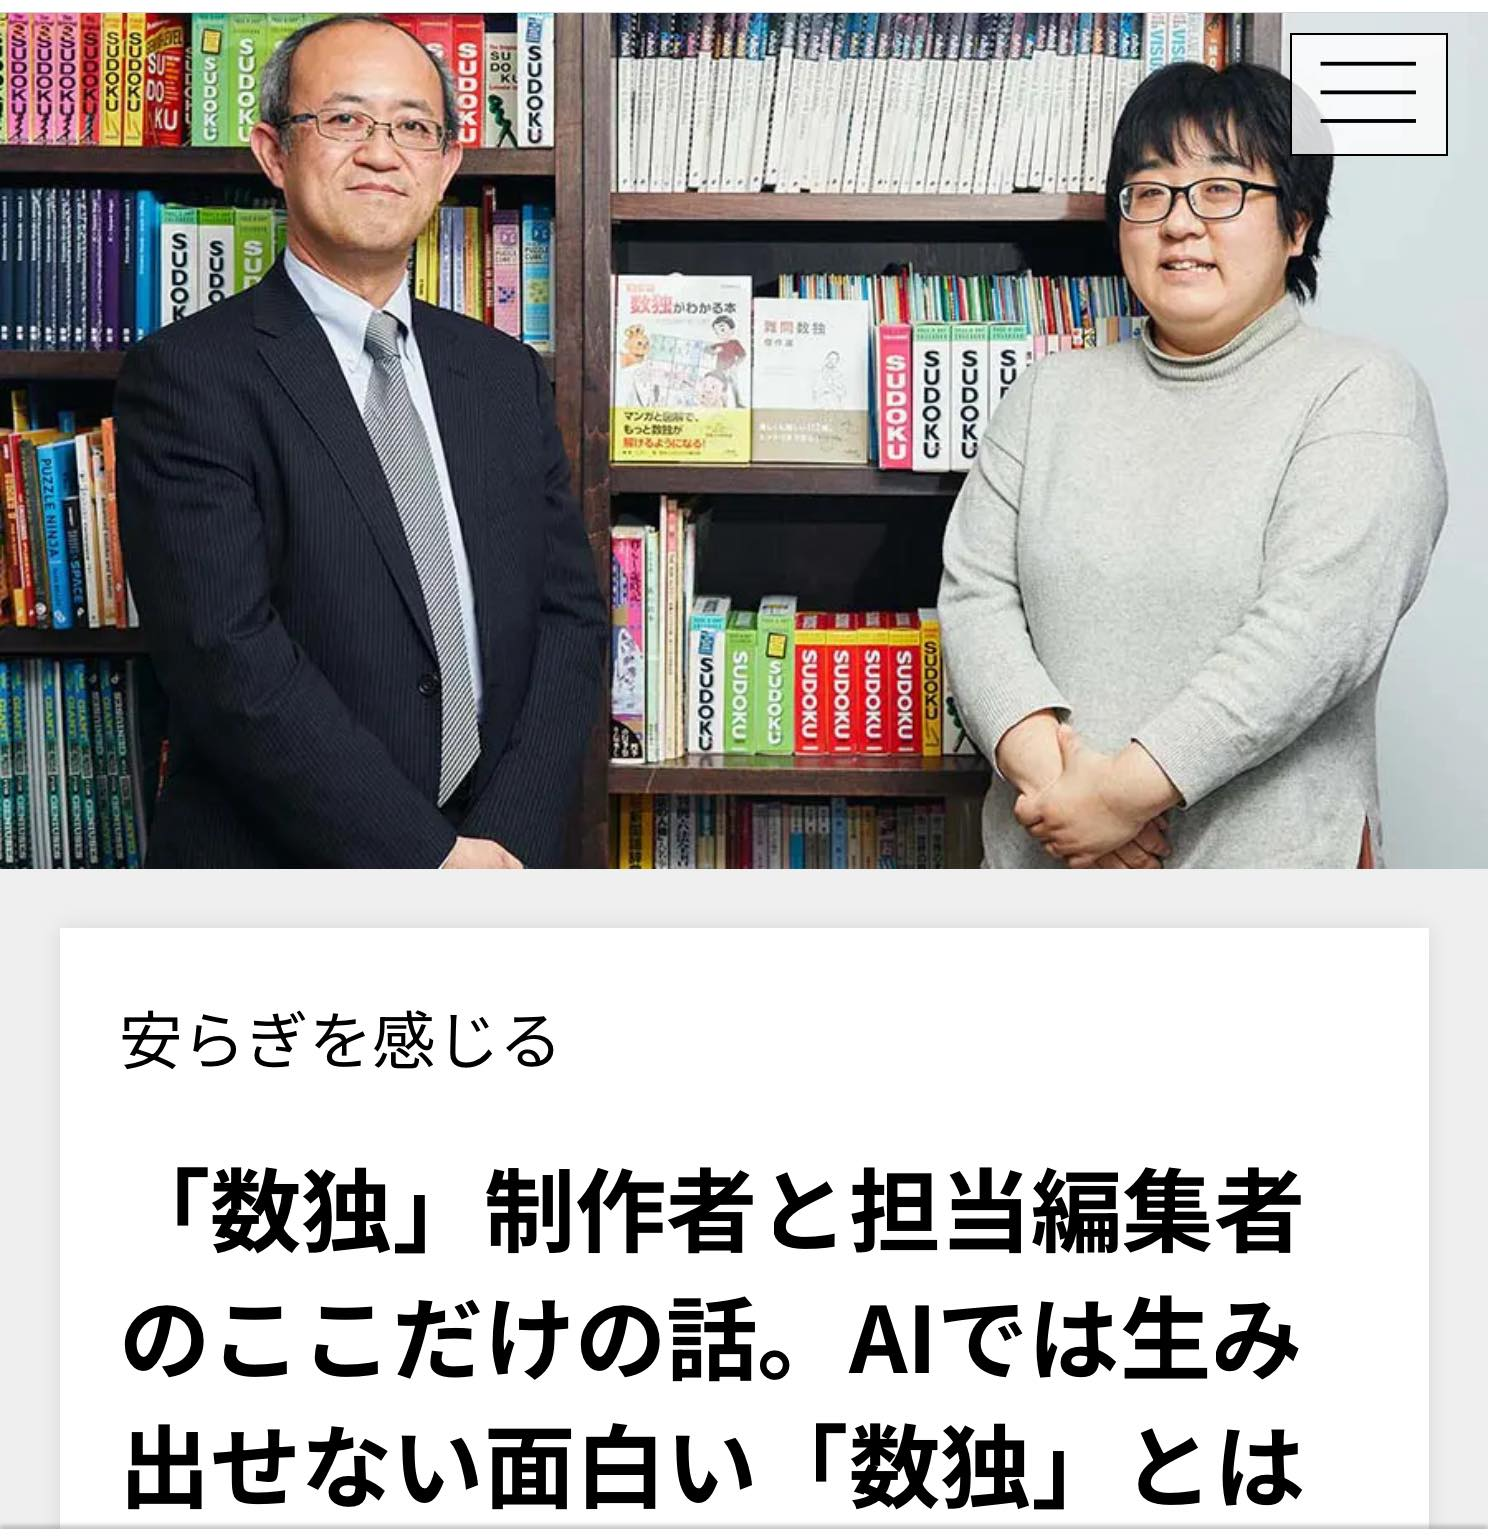
\includegraphics[width=\linewidth]{pictures/2025/05/20250501_085738_001.jpg}
\end{minipage}
\end{center}

\subsection*{2025年05月06日 08:44}
\addcontentsline{toc}{subsection}{2025年05月06日 08:44}

\url{https://youtu.be/EPxwolJ75pc}

\begin{center}
\href{https://youtu.be/EPxwolJ75pc}{
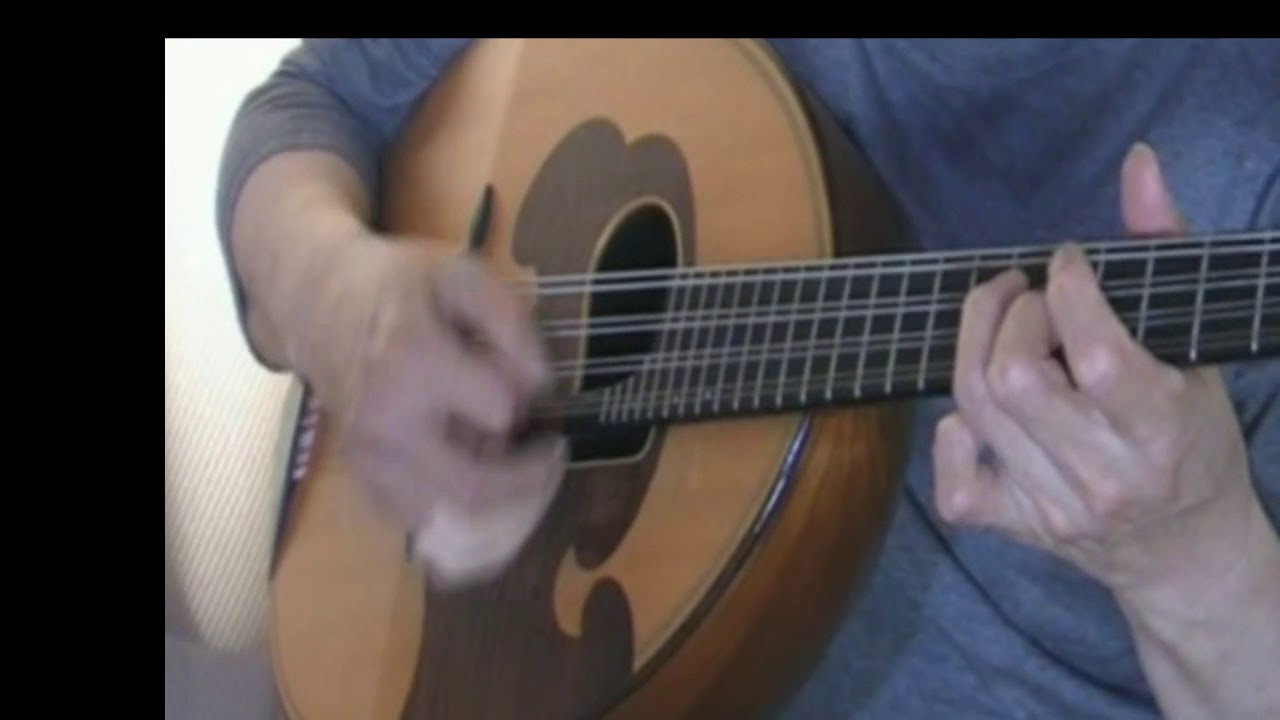
\includegraphics[width=0.48\linewidth]{pictures/youtube/2025/05/20250506_084429_youtube_001_EPxwolJ75pc.jpg}
}
\end{center}




マンドラって（思っていた以上に）良い音するんですねエ。

（これ本当にドラですか？チェロは？もっと大きかったですか？）

\subsection*{2025年05月06日 08:50}
\addcontentsline{toc}{subsection}{2025年05月06日 08:50}

\paragraph{リンク}
\url{https://youtu.be/Rv-0Yfs5vOg}

\begin{center}
\href{https://youtu.be/Rv-0Yfs5vOg}{
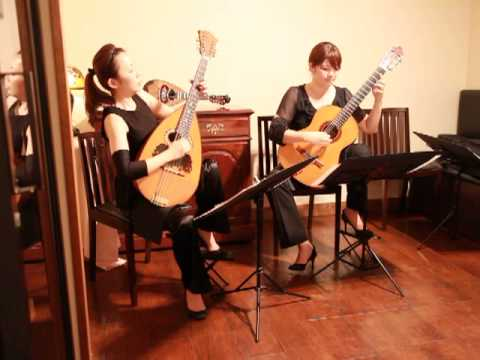
\includegraphics[width=0.48\linewidth]{pictures/youtube/2025/05/20250506_085019_youtube_001_Rv-0Yfs5vOg.jpg}
}
\end{center}

\subsection*{2025年05月06日 08:50}
\addcontentsline{toc}{subsection}{2025年05月06日 08:50}

\paragraph{リンク}
\url{https://youtu.be/W-lSFPRQ0Ow}

\begin{center}
\href{https://youtu.be/W-lSFPRQ0Ow}{
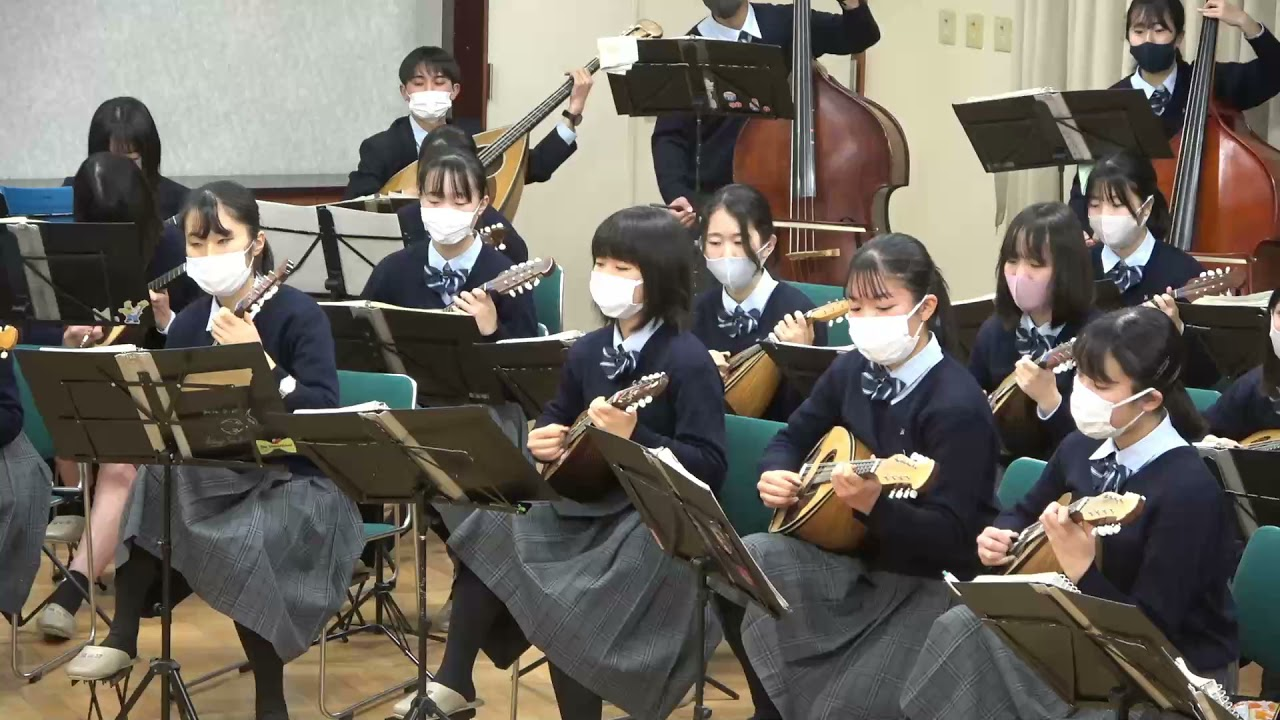
\includegraphics[width=0.48\linewidth]{pictures/youtube/2025/05/20250506_085059_youtube_001_W-lSFPRQ0Ow.jpg}
}
\end{center}

\subsection*{2025年05月06日 09:11}
\addcontentsline{toc}{subsection}{2025年05月06日 09:11}

\url{https://youtu.be/_D3Zmy7ygOQ}

\begin{center}
\href{https://youtu.be/_D3Zmy7ygOQ}{
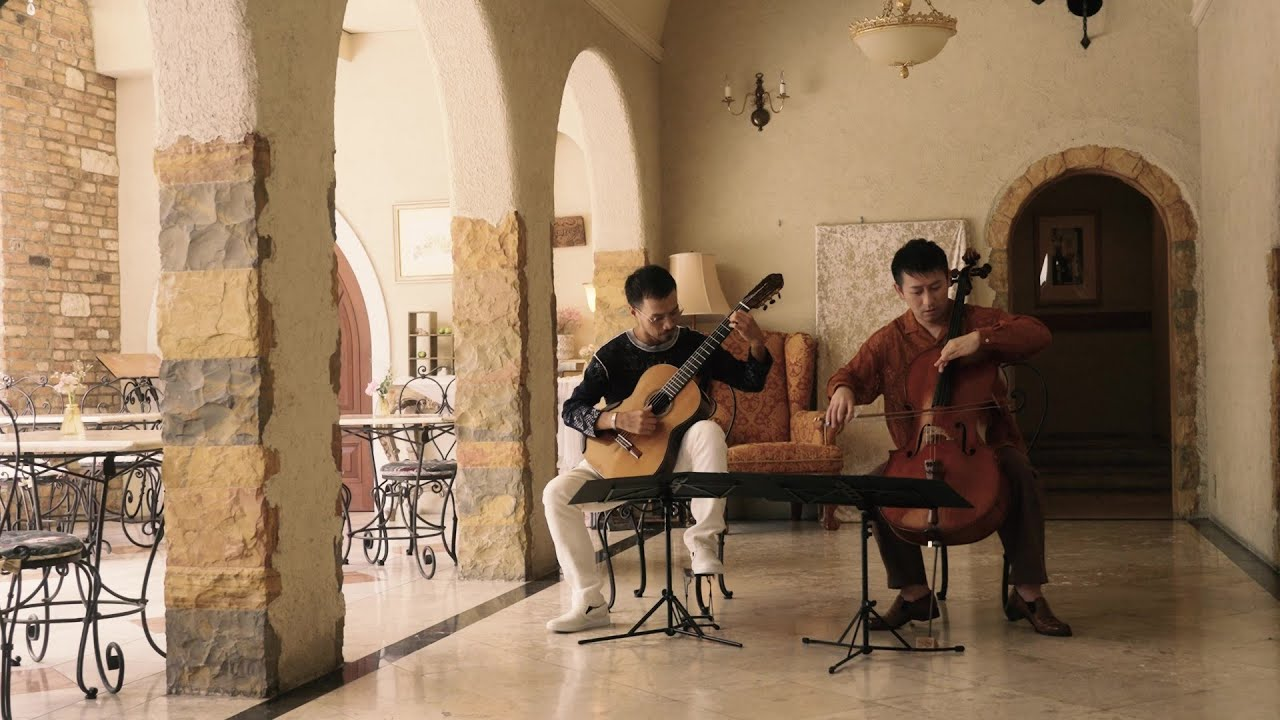
\includegraphics[width=0.48\linewidth]{pictures/youtube/2025/05/20250506_091111_youtube_001__D3Zmy7ygOQ.jpg}
}
\end{center}




\#紅の豚（5月9日夜9時〜金曜ロードショー）

「カッコイイとは、こういうことさ」


フランス🇫🇷語は何を言っているのか意味不明ですけど、何となくカッコいいと思って憧れていたことがあります。学生だった（教養部の）頃、第２外国語は独語をとりましたが、実は仏語の教室にコッソリ行って聞いていたことがあります。（急に当てられて何も答えられなかった覚えがありますが）唾を飛ばしながら喉から出すrの発音などとても出来るとは思えなかったな。


(１)単語の最後の子音字は基本的に発音しない（但し例外もある。フルートの教則本 \#Altes は、固有名詞なので最後のsは発音する。\#アルテス ですね。アルテではありません。）

(２)単語の最後の子音字は、続く単語の頭が母音字の場合には、 \#リエゾン して発音される

(３)C の下にヒゲの様な小さなSがチョコっとぶら下がっている文字（\#セディーユ）はSだと思って読む

(４)形容詞は、名詞を「後ろから」修飾する（昔、金沢城の大手門を出てすぐの所に、パント.ルージュという喫茶店があった。ルージュがパンツを修飾している。＊意味はあまり上品な話ではないので注意⚠）もちろん文法には例外がつきもの。ボー.ガットゥはボー（美しい）がガトゥ（お菓子）を前から修飾している（美しいお菓子＝ケーキの事）

(５)アルファベ（最後の子音字tを発音してはいけません）では、W（ドゥブルベ）、C（セ）、Y（イグレック）、H（アッシュ）、K（カー）など


フランスに旅行したらWC（ドゥブルベ.セ）を知っていたら役に立つとか、立たないとか


などなど、いくつか今でも断片的に覚えていることがあります。


\#宮田大、\#大萩康司

\subsection*{2025年05月06日 09:16}
\addcontentsline{toc}{subsection}{2025年05月06日 09:16}

\paragraph{リンク}
\url{https://youtu.be/-owD6Fbe7-8}

\begin{center}
\href{https://youtu.be/-owD6Fbe7-8}{
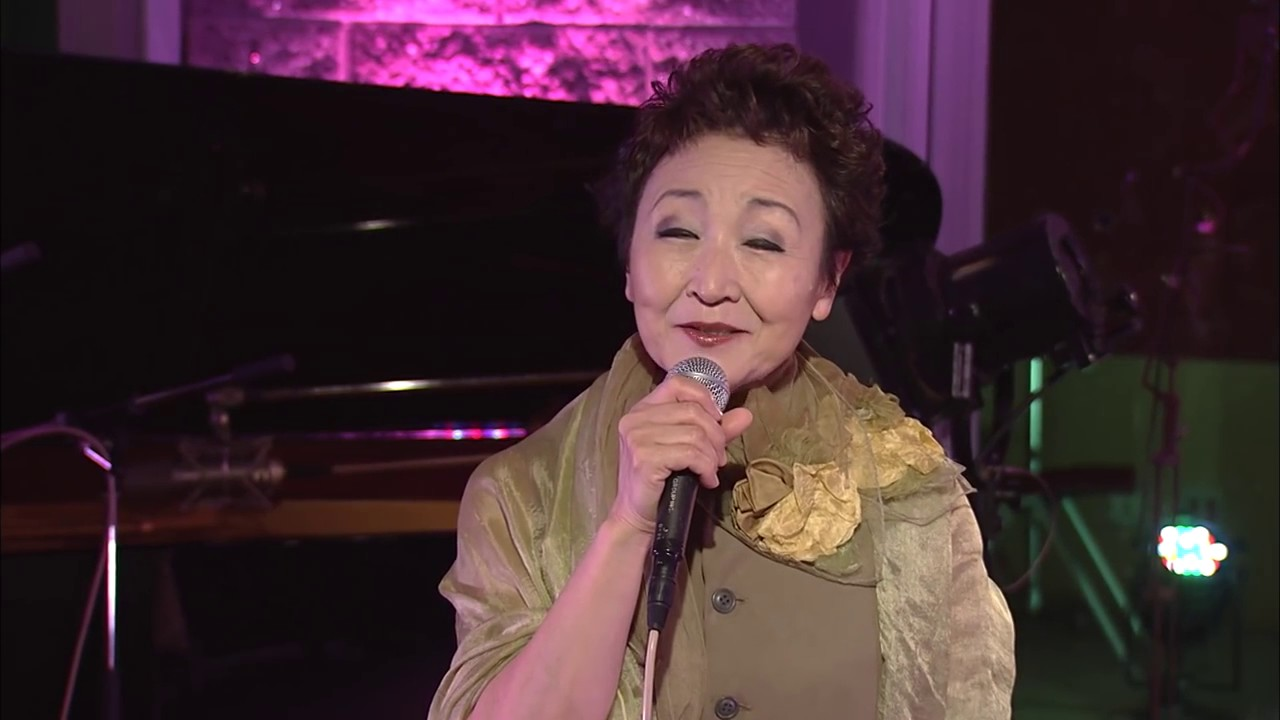
\includegraphics[width=0.48\linewidth]{pictures/youtube/2025/05/20250506_091629_youtube_001_-owD6Fbe7-8.jpg}
}
\end{center}

\subsection*{2025年05月06日 09:25}
\addcontentsline{toc}{subsection}{2025年05月06日 09:25}

\paragraph{リンク}
\url{https://youtu.be/lAEdsFk-xqQ}

\begin{center}
\href{https://youtu.be/lAEdsFk-xqQ}{
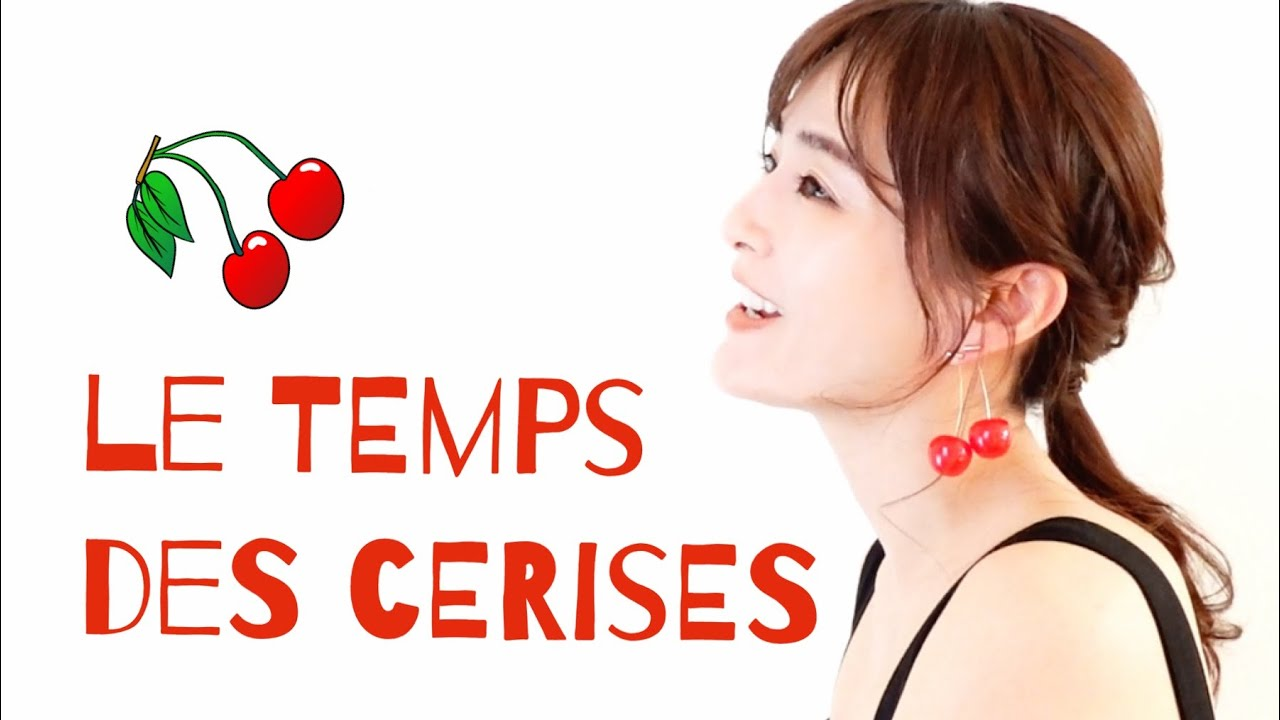
\includegraphics[width=0.48\linewidth]{pictures/youtube/2025/05/20250506_092505_youtube_001_lAEdsFk-xqQ.jpg}
}
\end{center}

\subsection*{2025年05月06日 10:46}
\addcontentsline{toc}{subsection}{2025年05月06日 10:46}

六畳の部屋に \#スポットクーラー なるものを導入しています。（今年もその季節が近づいてきました）


メーカーの想定ではサッシを半開き（開いて隙間を作って）にして、そこに穴の空いた縦長の板を挟み込み、その板の穴に \#吸排気 用の \#ダクト を繋ぐというものでした。しかし、\#サッシ を半開きのままにしておくのもチョットねえと思っていた所、


丁度良い程あいの \#小窓 がサッシの上部に「既にある」ことに気づいた。


この小窓を使って \#吸気 と \#排気 をできないかと思い、 \#3Dプリンタ で 小窓用吸排気口なる物を作ってみることにした。


サッシ小窓の表と裏から挟み込む様にして固定する形にしています。表裏それぞれの印刷に３時間から４時間半ほどかかっている（宙に浮いてる部分のサポート部の印刷に時間がかかっている。雨避け部を無くせば短時間で済むと思います）。吸気用と排気用で二対必要ですから、3Dプリンタでの印刷には（試行錯誤もあって）３日ほどかかりました。その間、ダクトを覆う遮熱用カバーやドレン水を貯めるポリタンクも用意して、最終的には（思いの他）良い状態になったのではないかと思っています。（ \#トヨトミ の TAD-22 xx用です）

\paragraph{写真}
\begin{center}
\begin{minipage}{0.48\linewidth}
\centering
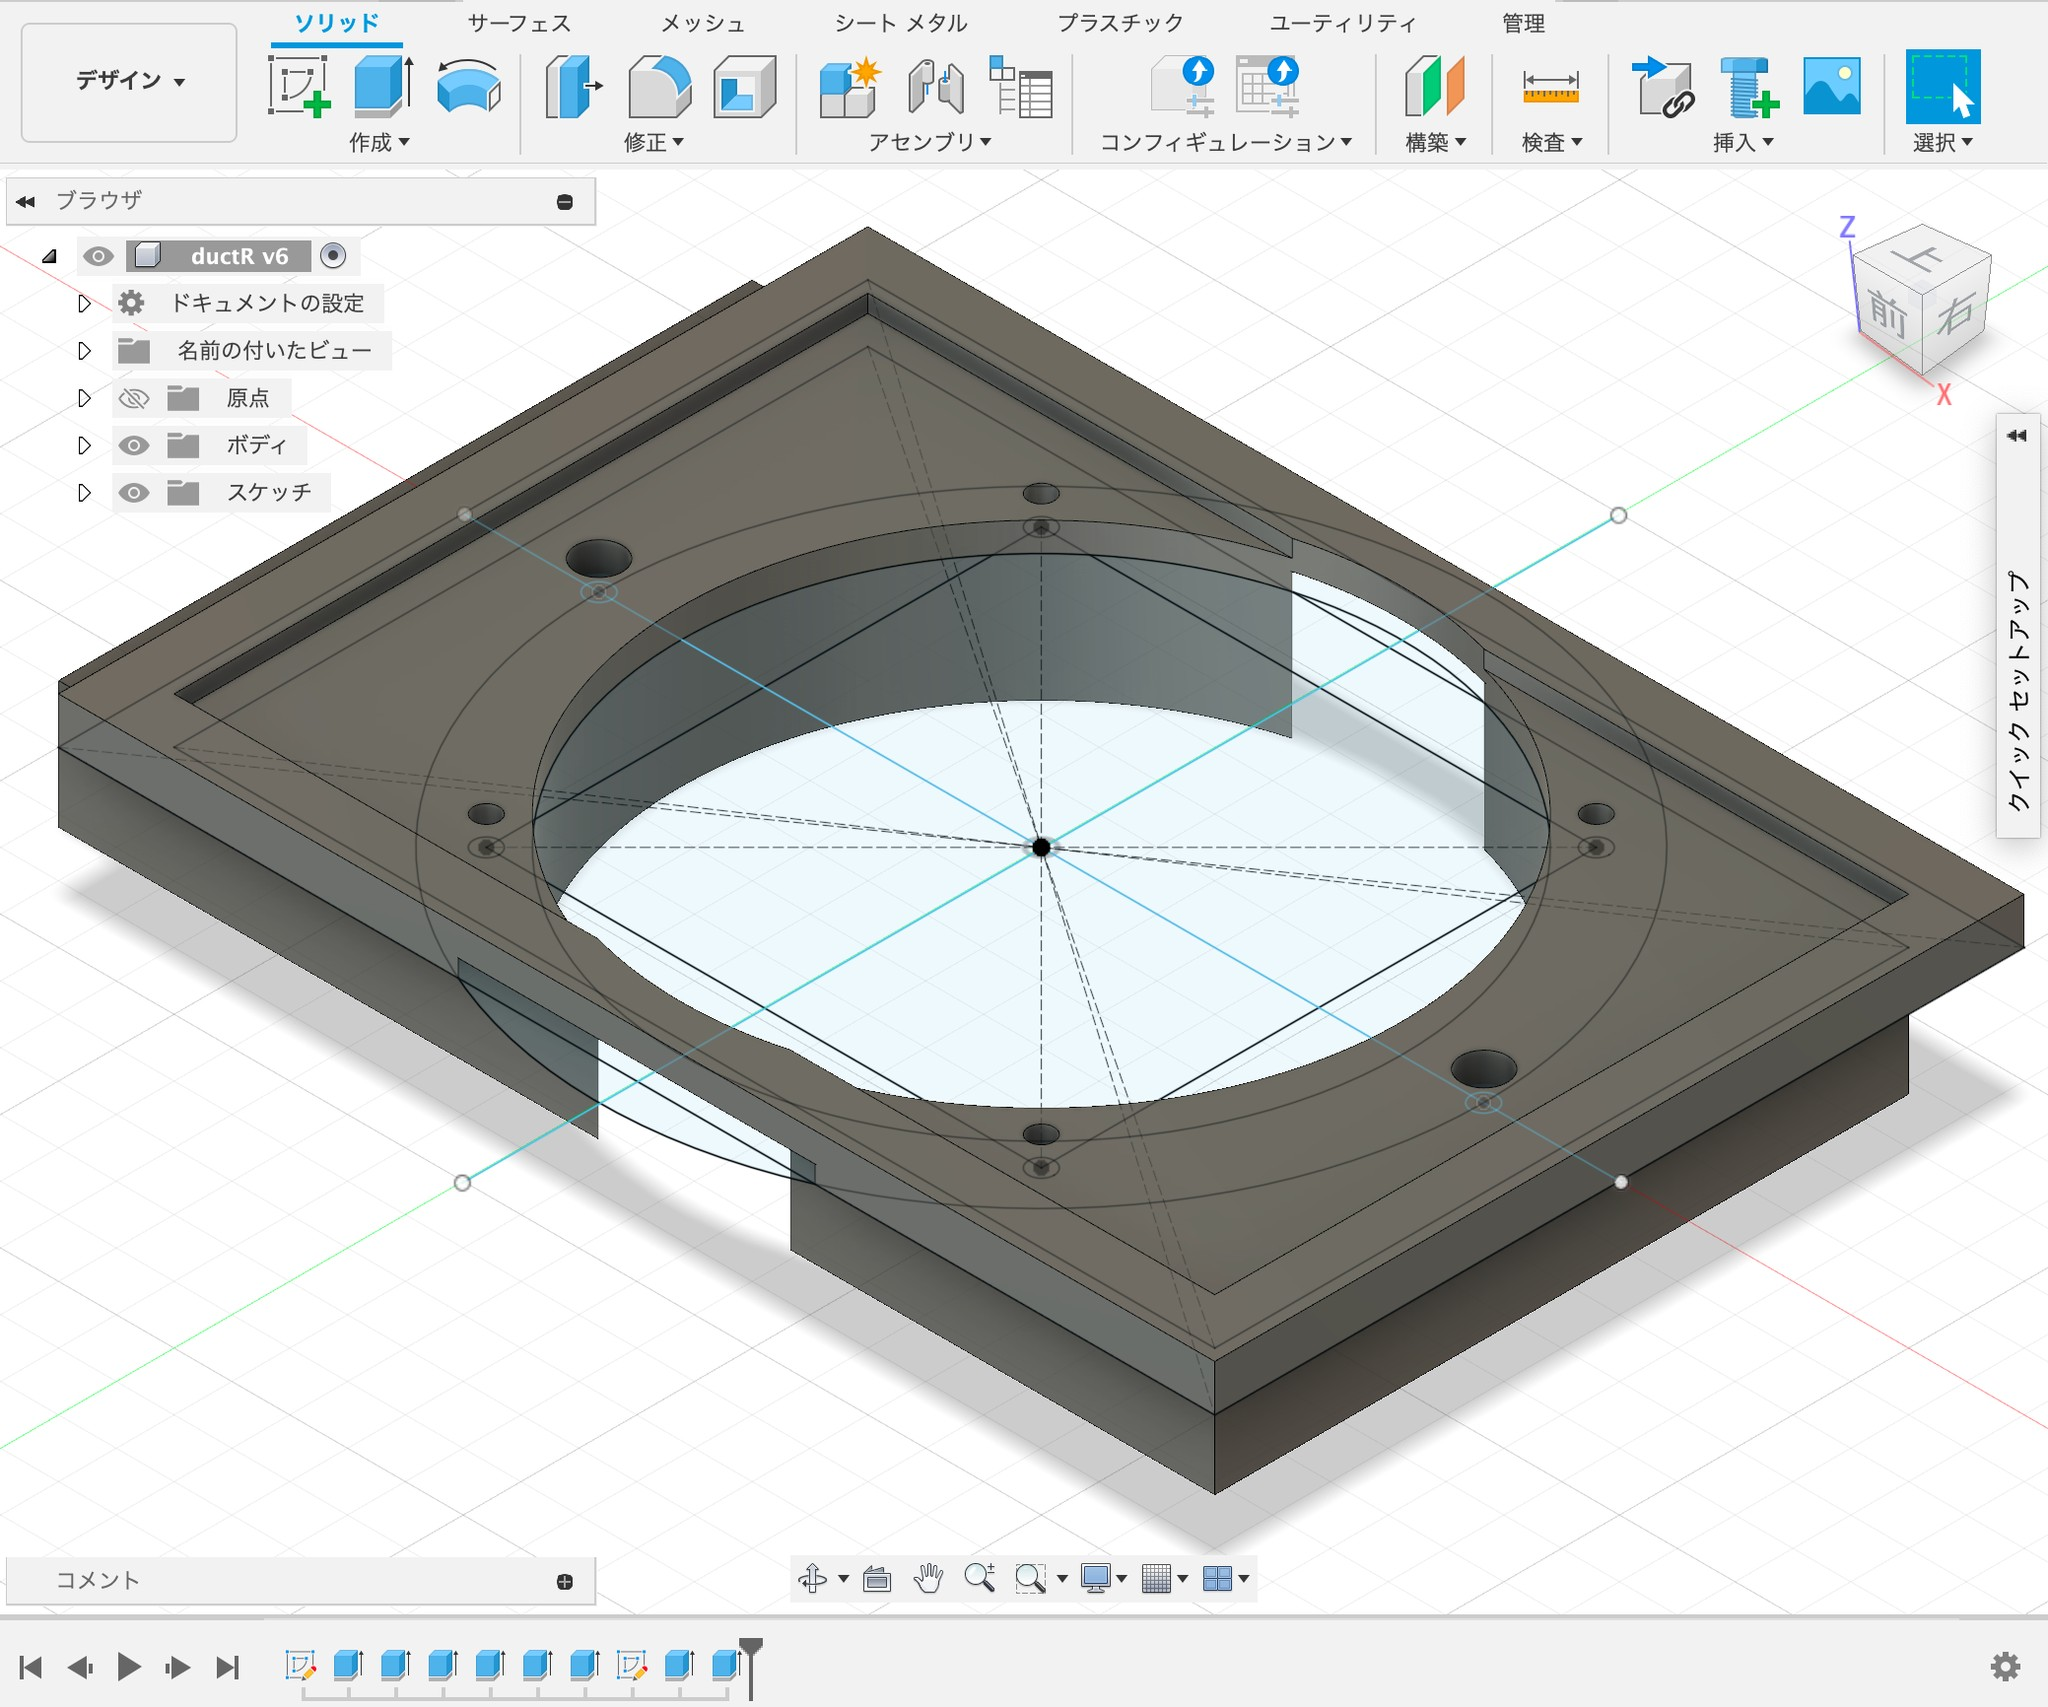
\includegraphics[width=\linewidth]{pictures/2025/05/20250506_104654_001.jpg}
\end{minipage}
\hfill
\begin{minipage}{0.48\linewidth}
\centering
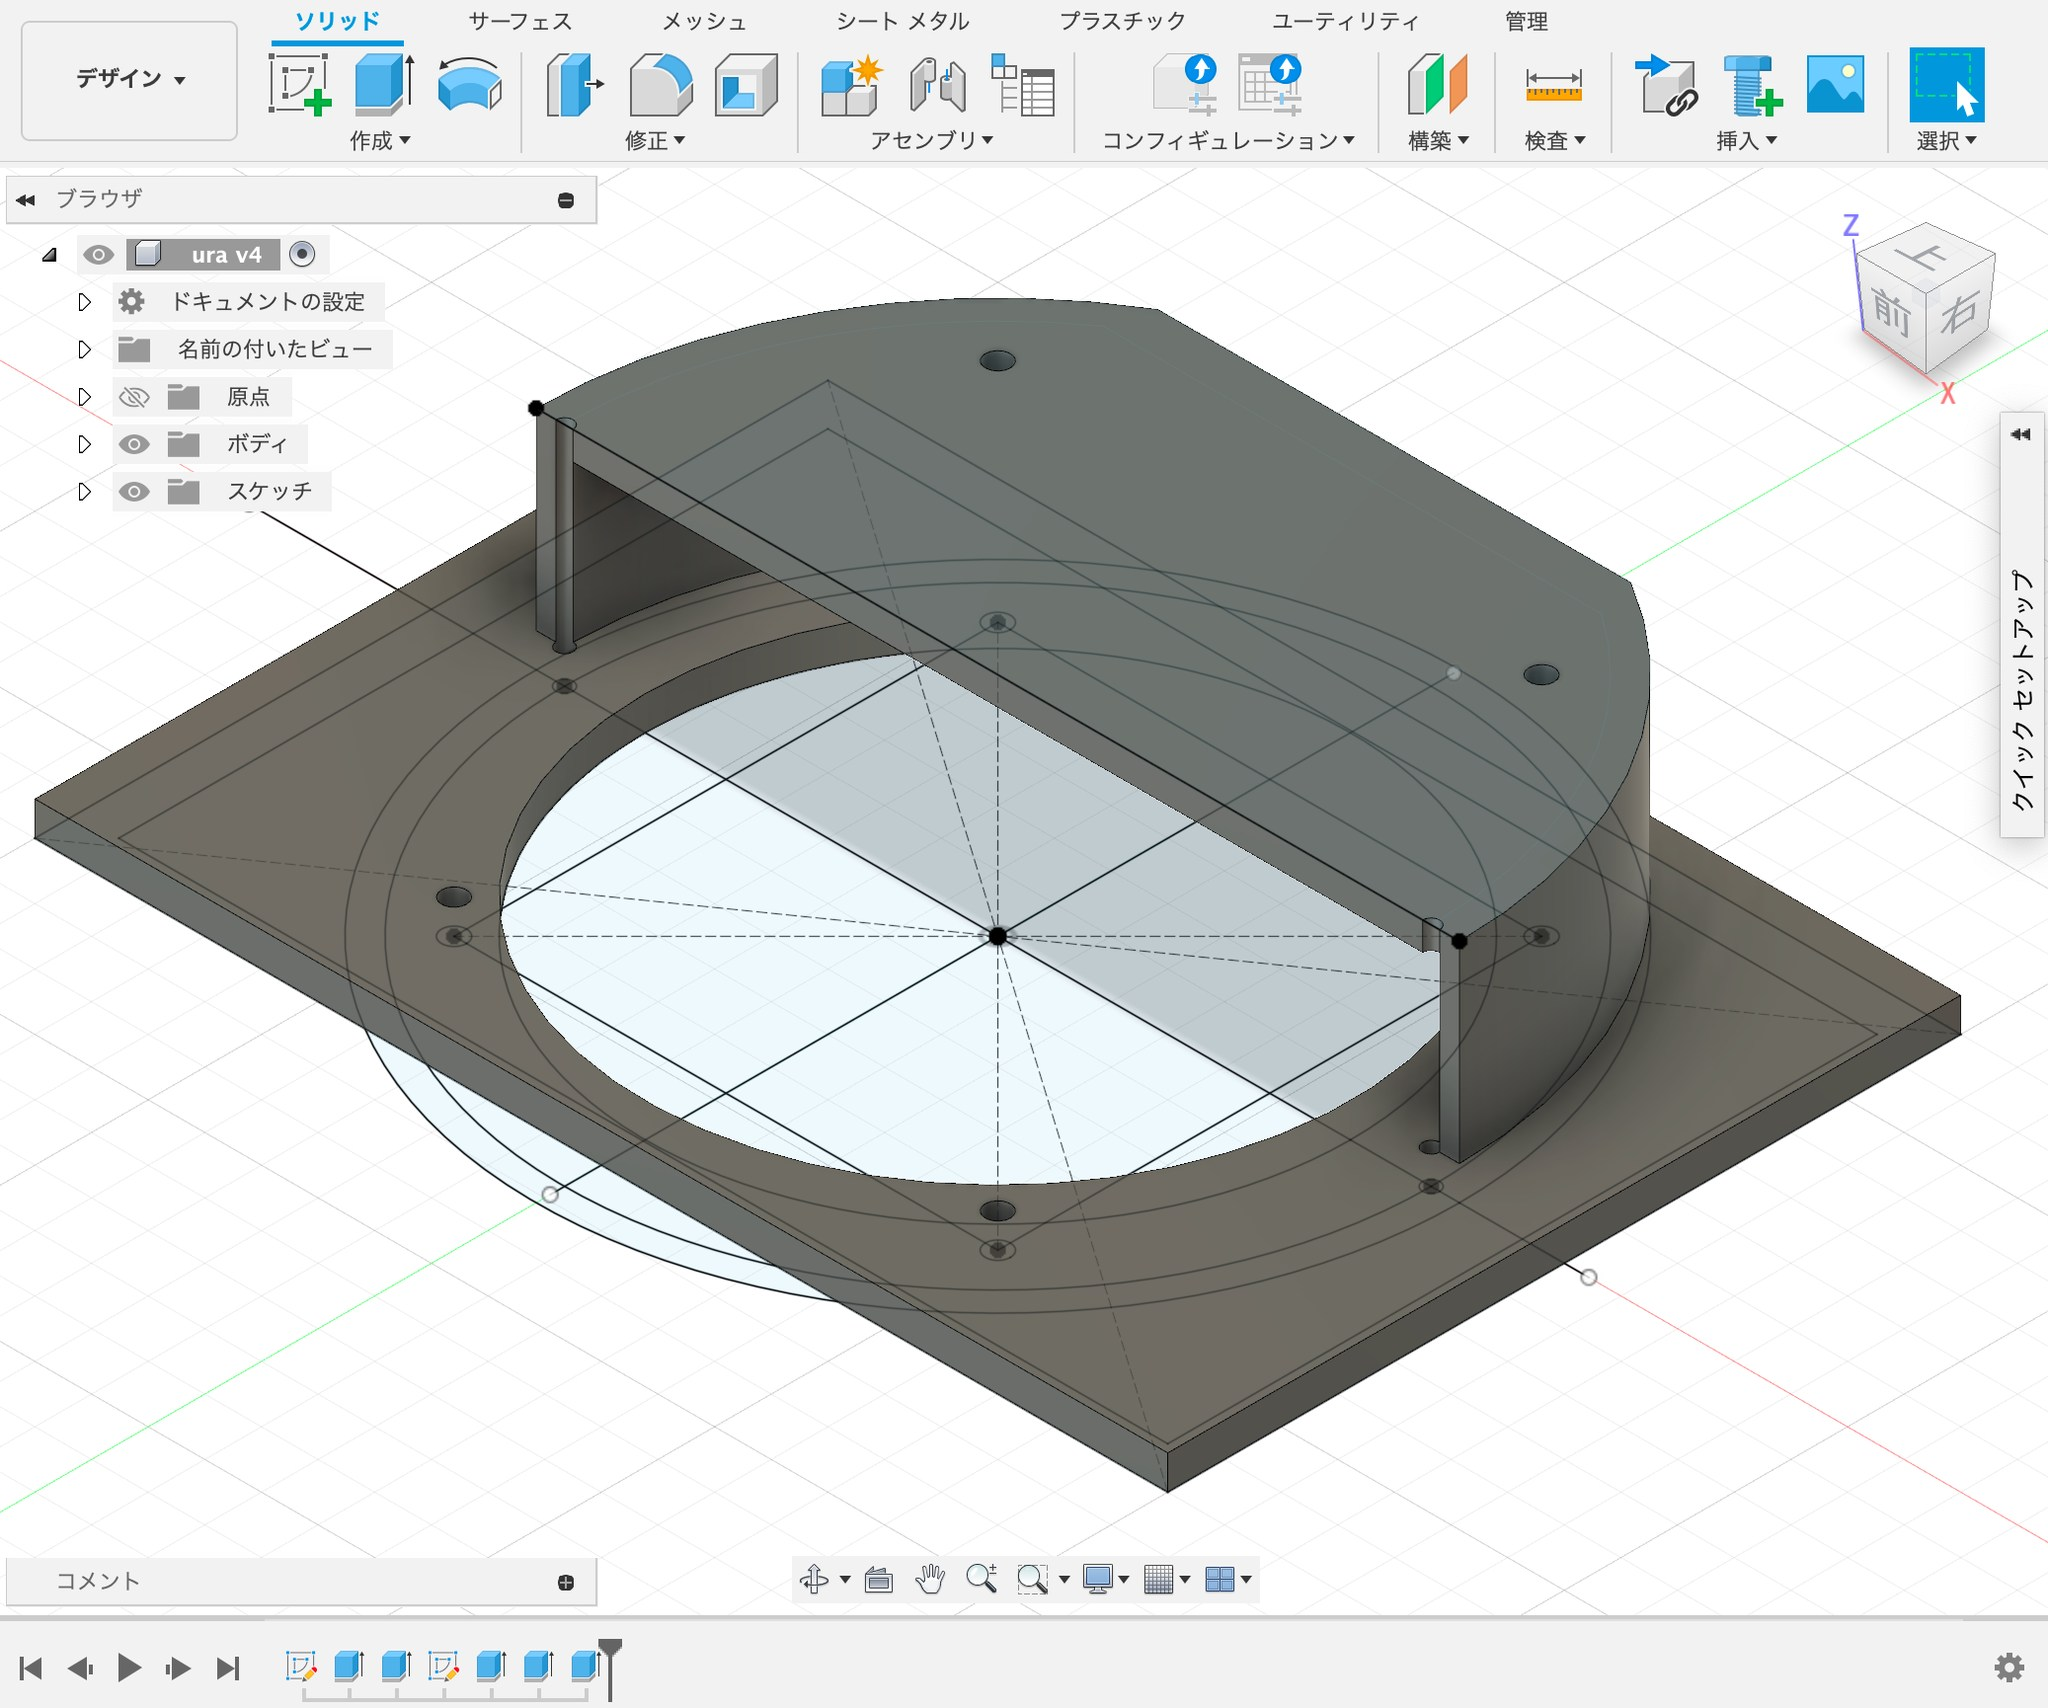
\includegraphics[width=\linewidth]{pictures/2025/05/20250506_104654_002.jpg}
\end{minipage}
\end{center}

\begin{center}
\begin{minipage}{0.48\linewidth}
\centering
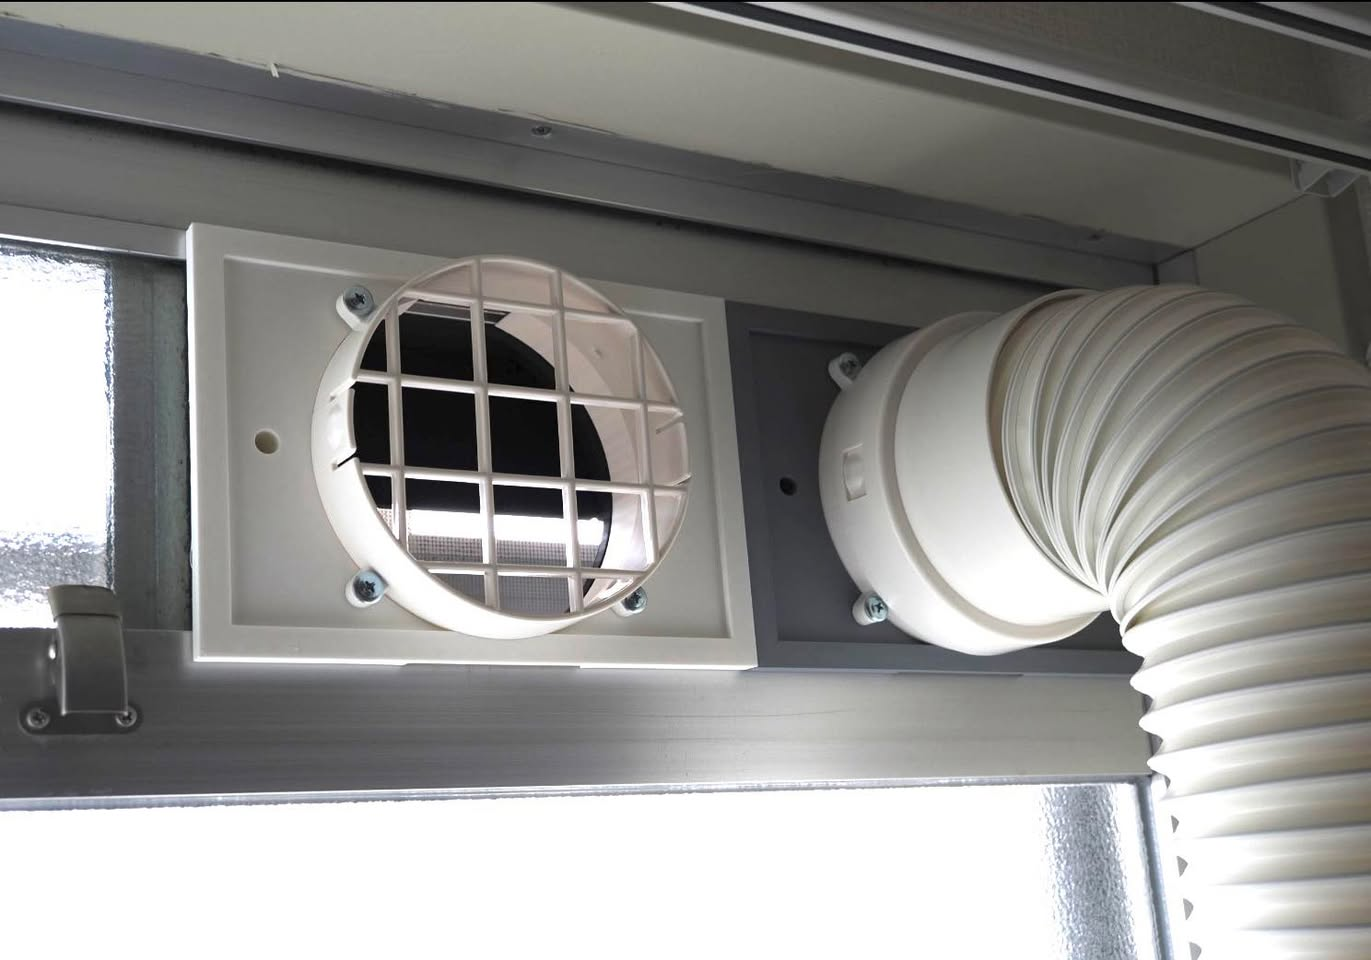
\includegraphics[width=\linewidth]{pictures/2025/05/20250506_104654_003.jpg}
\end{minipage}
\hfill
\begin{minipage}{0.48\linewidth}
\centering
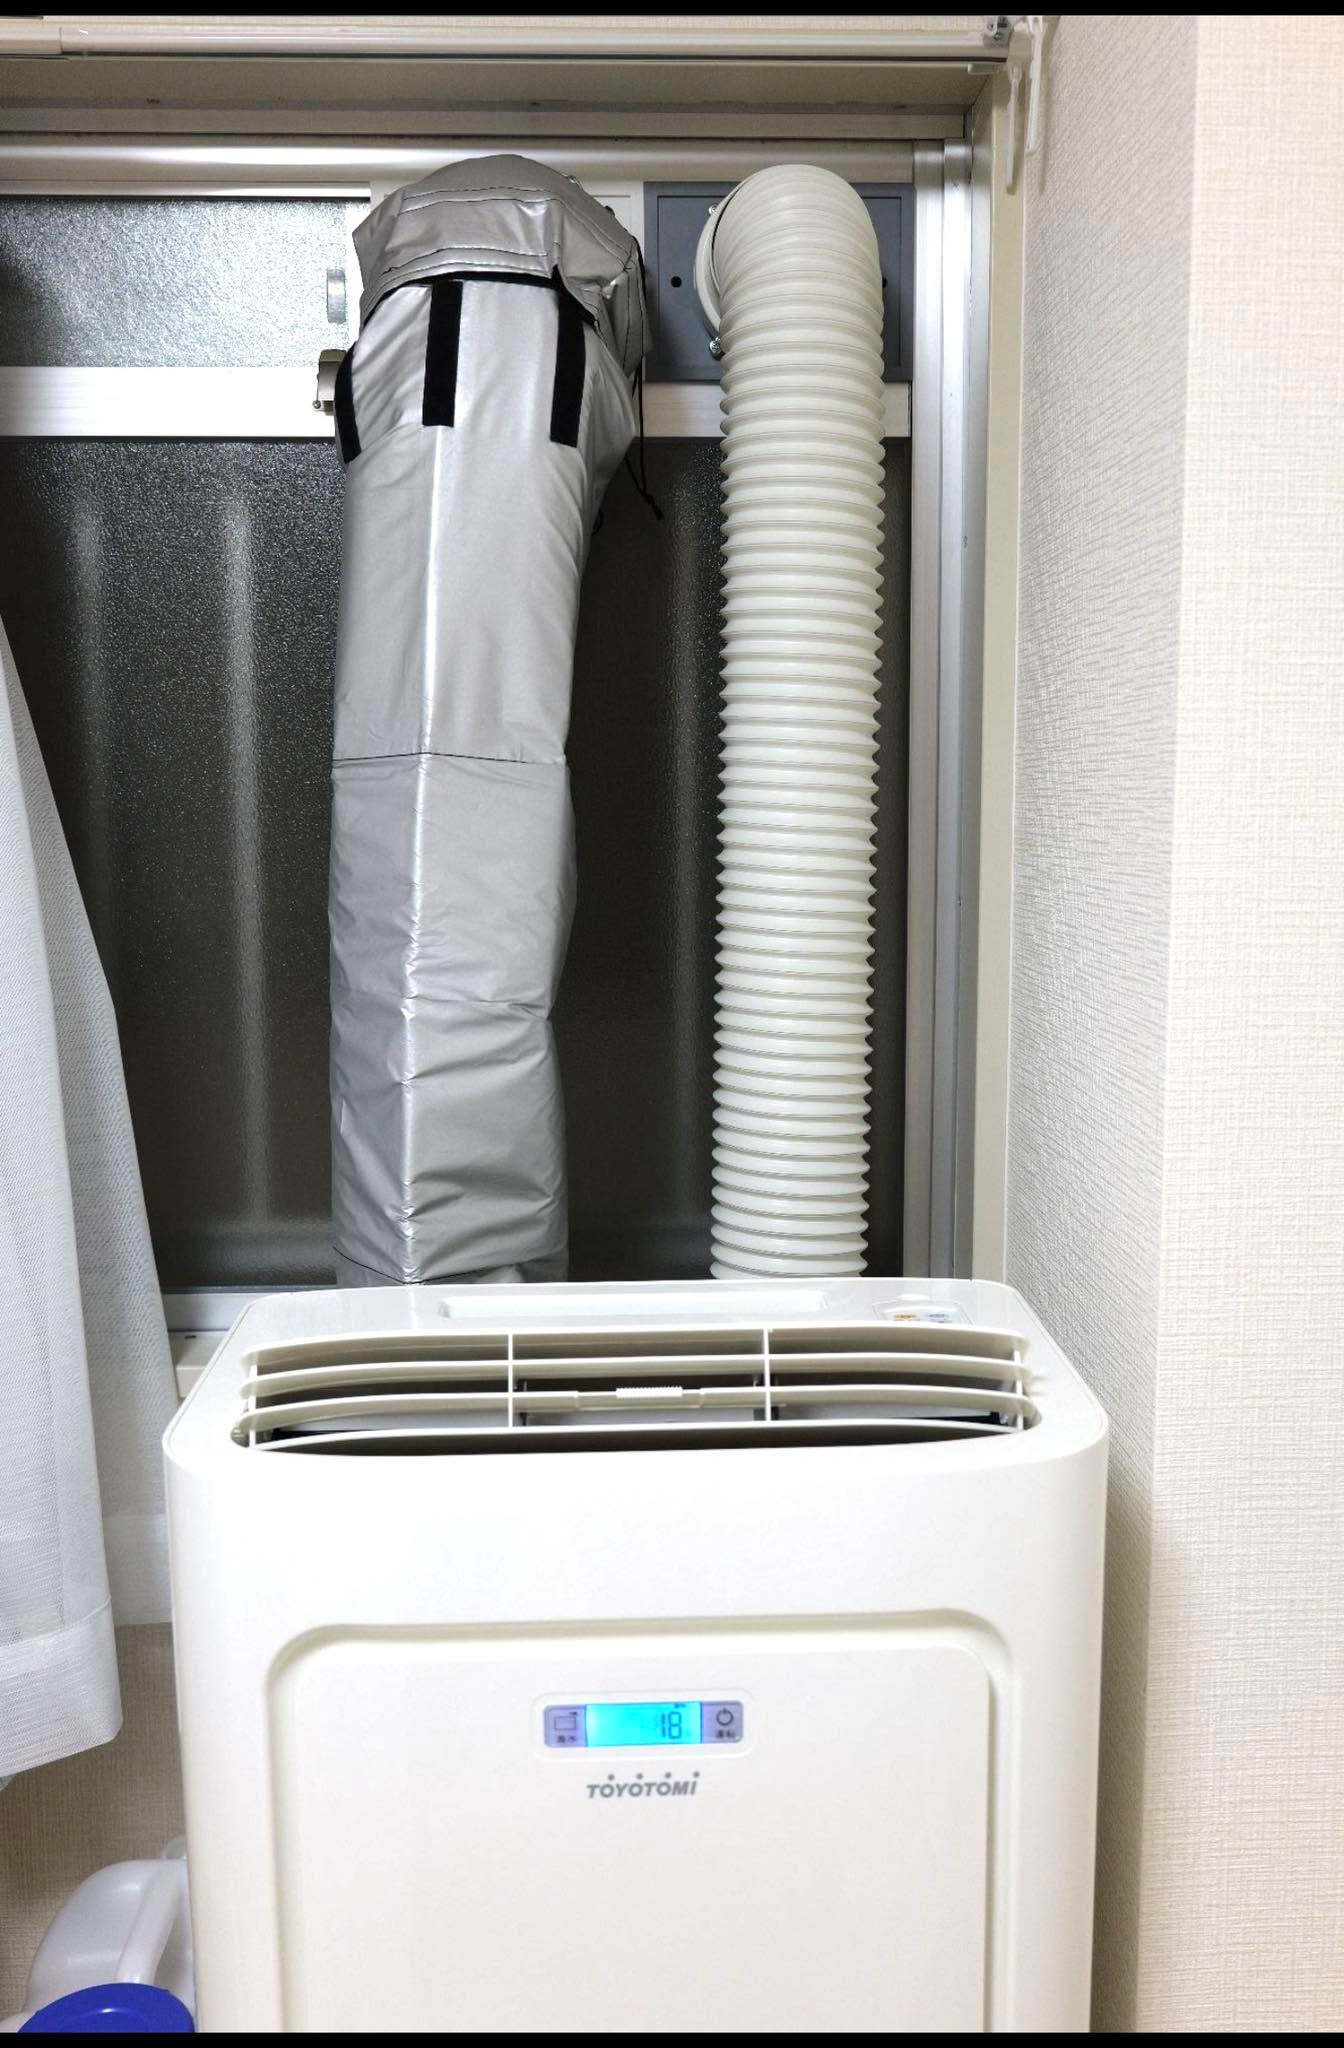
\includegraphics[width=\linewidth]{pictures/2025/05/20250506_104654_004.jpg}
\end{minipage}
\end{center}

\subsection*{2025年05月06日 16:48}
\addcontentsline{toc}{subsection}{2025年05月06日 16:48}

\paragraph{リンク}
\url{https://youtu.be/mkgoaC1XKU4}

\begin{center}
\href{https://youtu.be/mkgoaC1XKU4}{
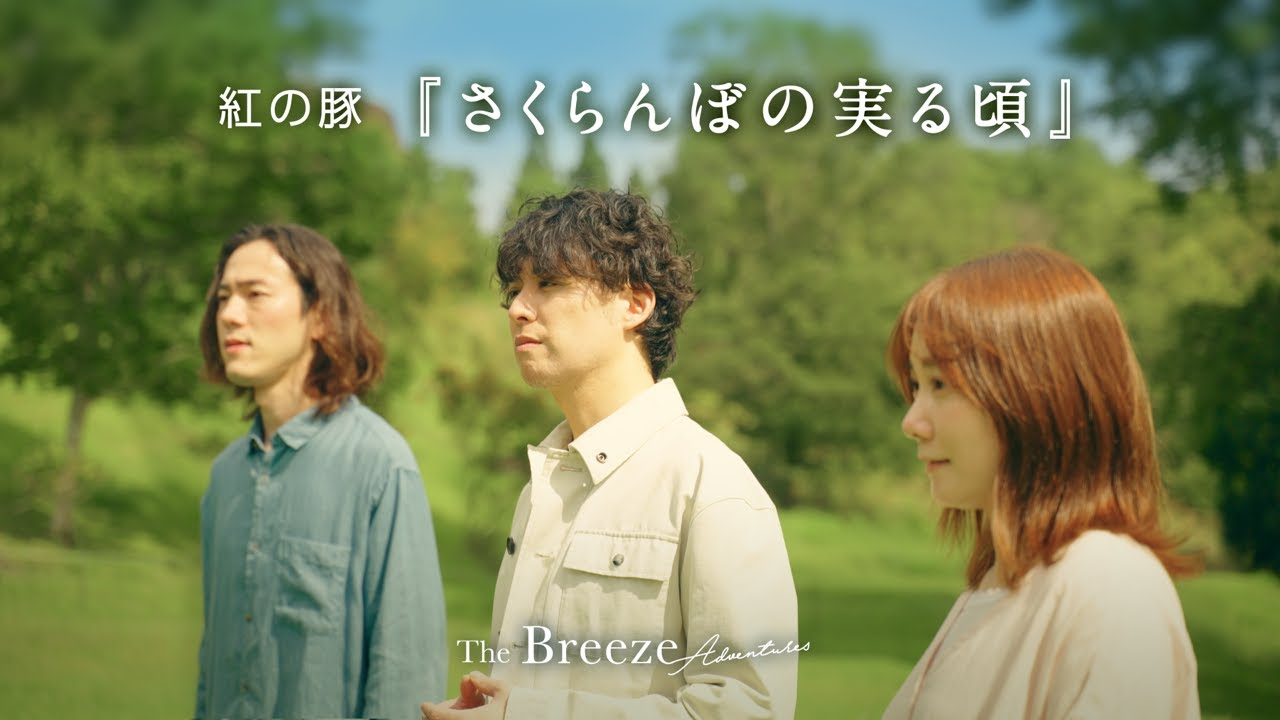
\includegraphics[width=0.48\linewidth]{pictures/youtube/2025/05/20250506_164813_youtube_001_mkgoaC1XKU4.jpg}
}
\end{center}

\subsection*{2025年05月06日 17:28}
\addcontentsline{toc}{subsection}{2025年05月06日 17:28}

\paragraph{リンク}
\url{https://youtu.be/Uy9PsKAu-wU}

\begin{center}
\href{https://youtu.be/Uy9PsKAu-wU}{
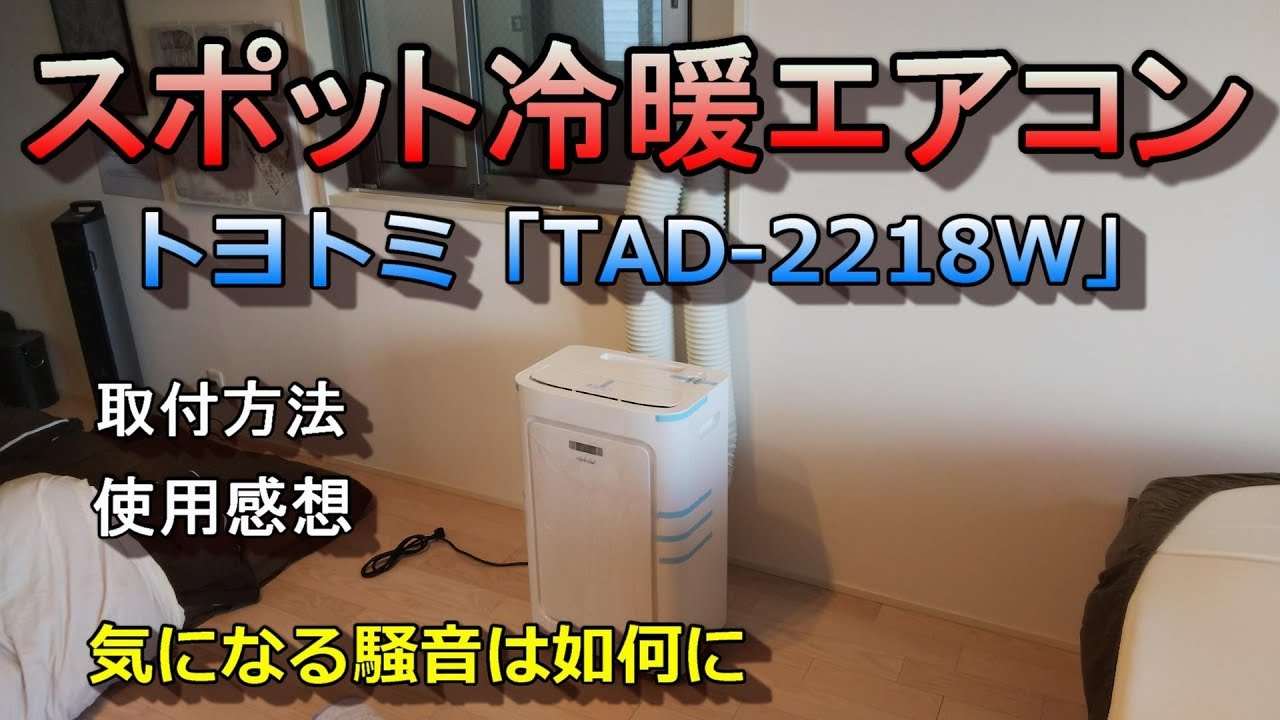
\includegraphics[width=0.48\linewidth]{pictures/youtube/2025/05/20250506_172838_youtube_001_Uy9PsKAu-wU.jpg}
}
\end{center}

\subsection*{2025年05月06日 20:09}
\addcontentsline{toc}{subsection}{2025年05月06日 20:09}

\paragraph{リンク}
\url{https://youtu.be/olR0n3vbN70}

\begin{center}
\href{https://youtu.be/olR0n3vbN70}{

\includegraphics[width=0.48\linewidth]{pictures/youtube/2025/05/20250506_200955_youtube_001_olR0n3vbN70.jpg}
}
\end{center}

\subsection*{2025年05月06日 20:19}
\addcontentsline{toc}{subsection}{2025年05月06日 20:19}

\paragraph{リンク}
\url{https://youtu.be/jI-MI18EpbU}

\begin{center}
\href{https://youtu.be/jI-MI18EpbU}{
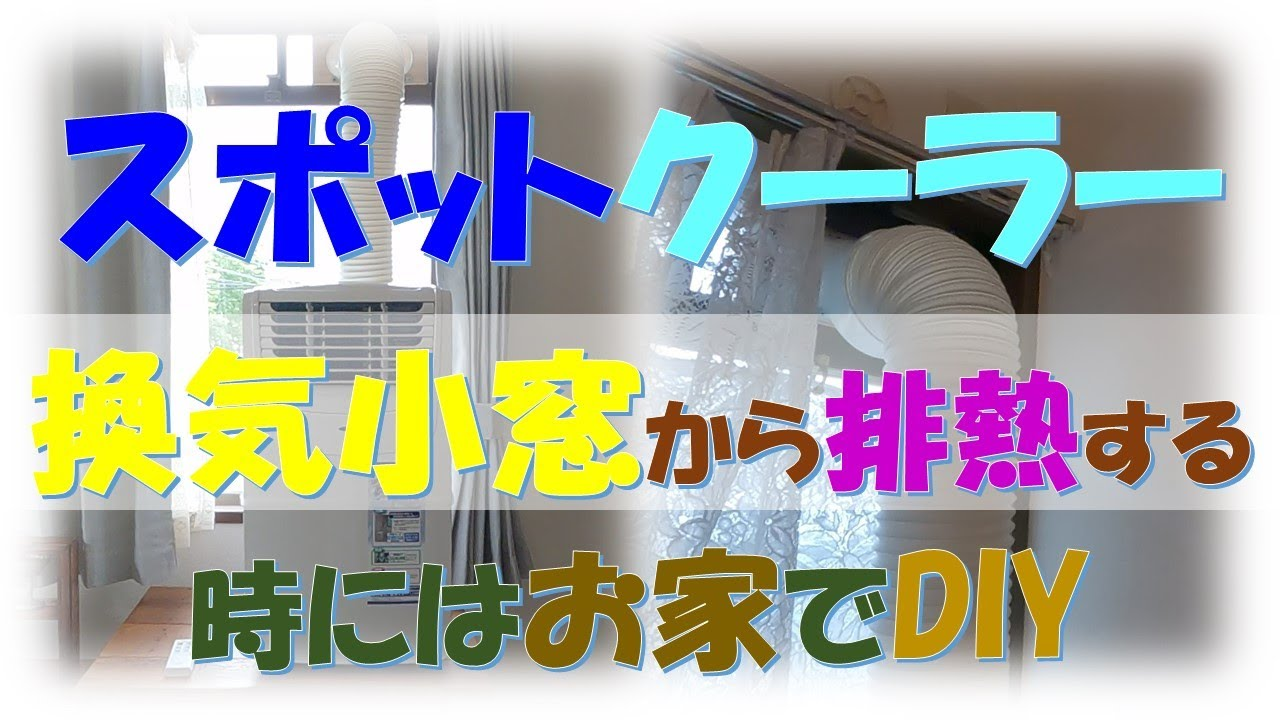
\includegraphics[width=0.48\linewidth]{pictures/youtube/2025/05/20250506_201903_youtube_001_jI-MI18EpbU.jpg}
}
\end{center}

\subsection*{2025年05月07日 02:11}
\addcontentsline{toc}{subsection}{2025年05月07日 02:11}

\url{https://youtu.be/WWw3Po1wOtE}

\begin{center}
\href{https://youtu.be/WWw3Po1wOtE}{
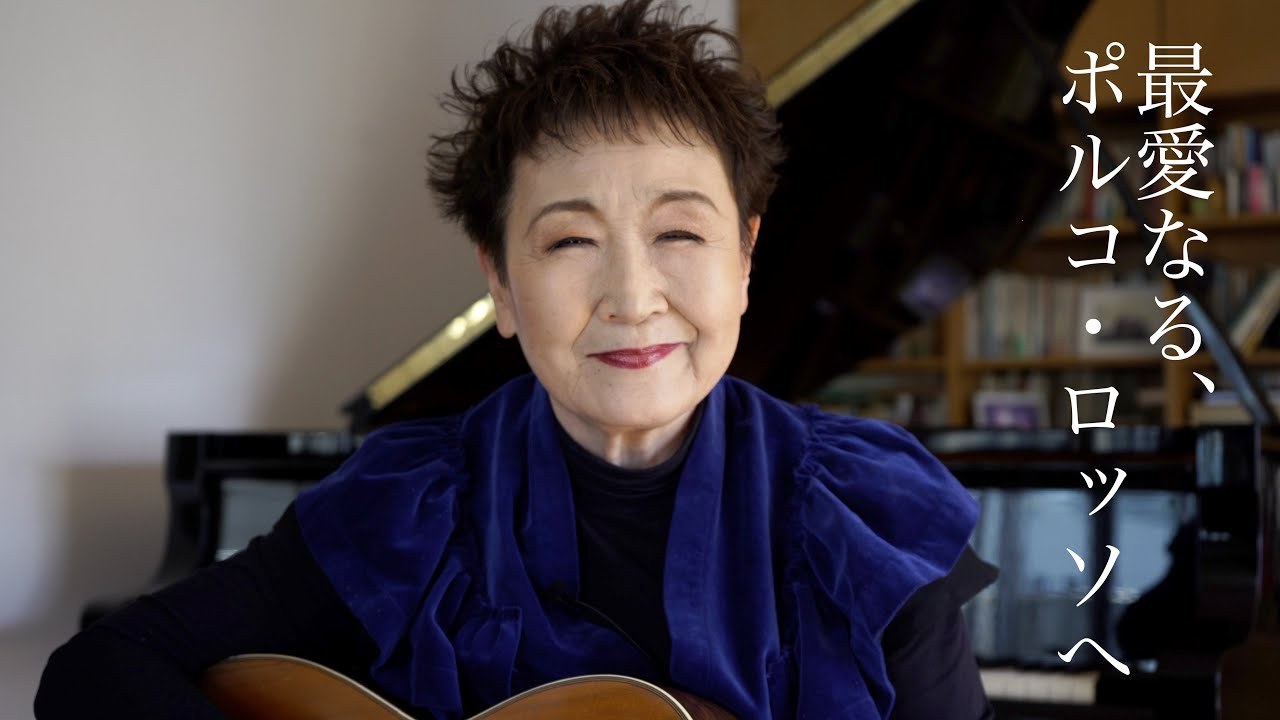
\includegraphics[width=0.48\linewidth]{pictures/youtube/2025/05/20250507_021144_youtube_001_WWw3Po1wOtE.jpg}
}
\end{center}




\#紅の豚（5月9日夜9時〜金曜ロードショー）

「飛ばねえ豚はただの豚だ」


時には昔の話をしようか

．．．

あの日の全てが虚しいものだと

それは誰にも言えない

今でも同じ様に見果てぬ夢を描いて

走り続けているよね

何処かで

．．．


人生の黄昏時に聞くと、「そうだね」って言いたくなる。

\subsection*{2025年05月07日 02:12}
\addcontentsline{toc}{subsection}{2025年05月07日 02:12}

\paragraph{リンク}
\url{https://youtu.be/3Q2FmlLJxCQ}

\begin{center}
\href{https://youtu.be/3Q2FmlLJxCQ}{
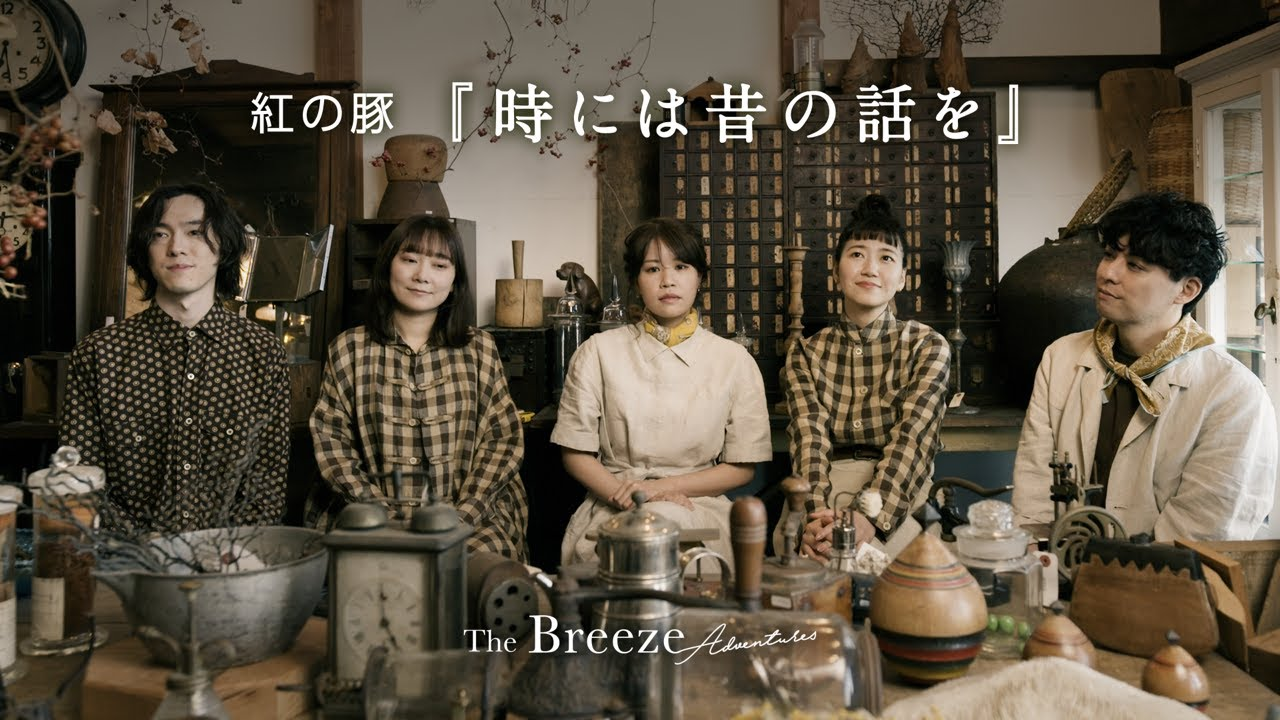
\includegraphics[width=0.48\linewidth]{pictures/youtube/2025/05/20250507_021238_youtube_001_3Q2FmlLJxCQ.jpg}
}
\end{center}

\subsection*{2025年05月07日 02:14}
\addcontentsline{toc}{subsection}{2025年05月07日 02:14}

\paragraph{リンク}
\url{https://youtu.be/WWw3Po1wOtE}

\begin{center}
\href{https://youtu.be/WWw3Po1wOtE}{
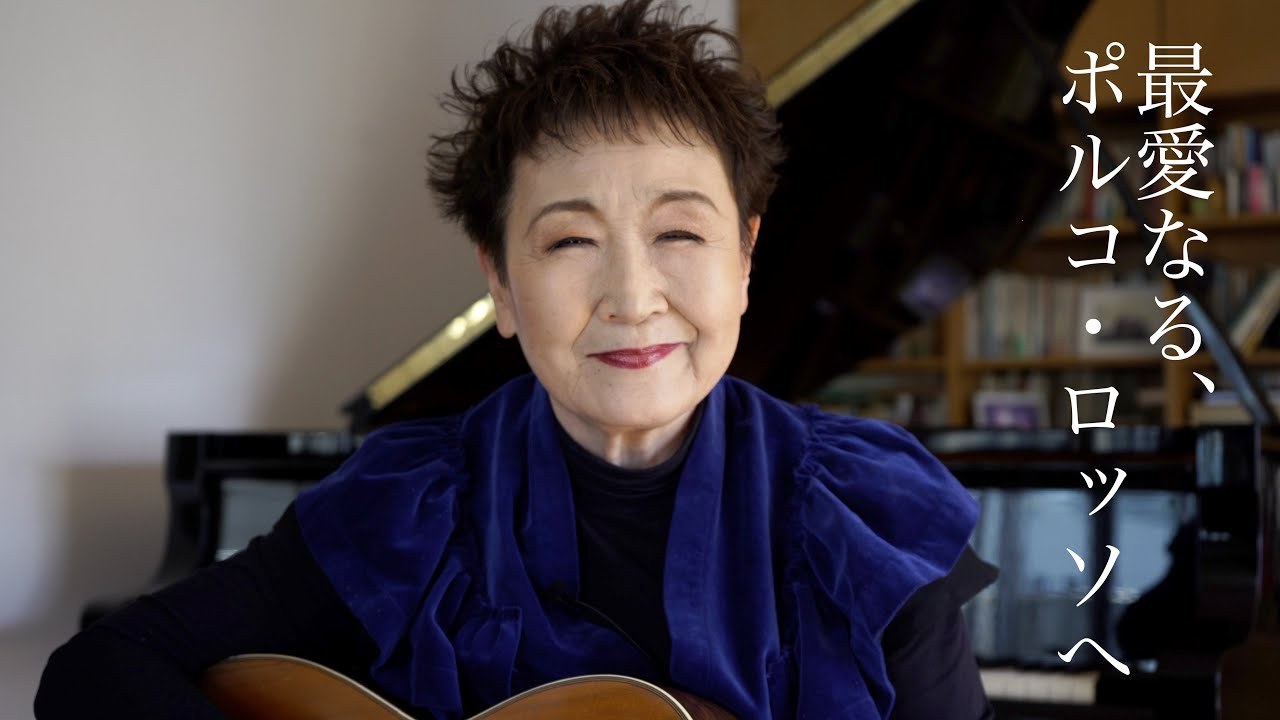
\includegraphics[width=0.48\linewidth]{pictures/youtube/2025/05/20250507_021419_youtube_001_WWw3Po1wOtE.jpg}
}
\end{center}

\subsection*{2025年05月07日 02:14}
\addcontentsline{toc}{subsection}{2025年05月07日 02:14}

\paragraph{リンク}
\url{https://youtu.be/Ny7W8D2CPEc}

\begin{center}
\href{https://youtu.be/Ny7W8D2CPEc}{
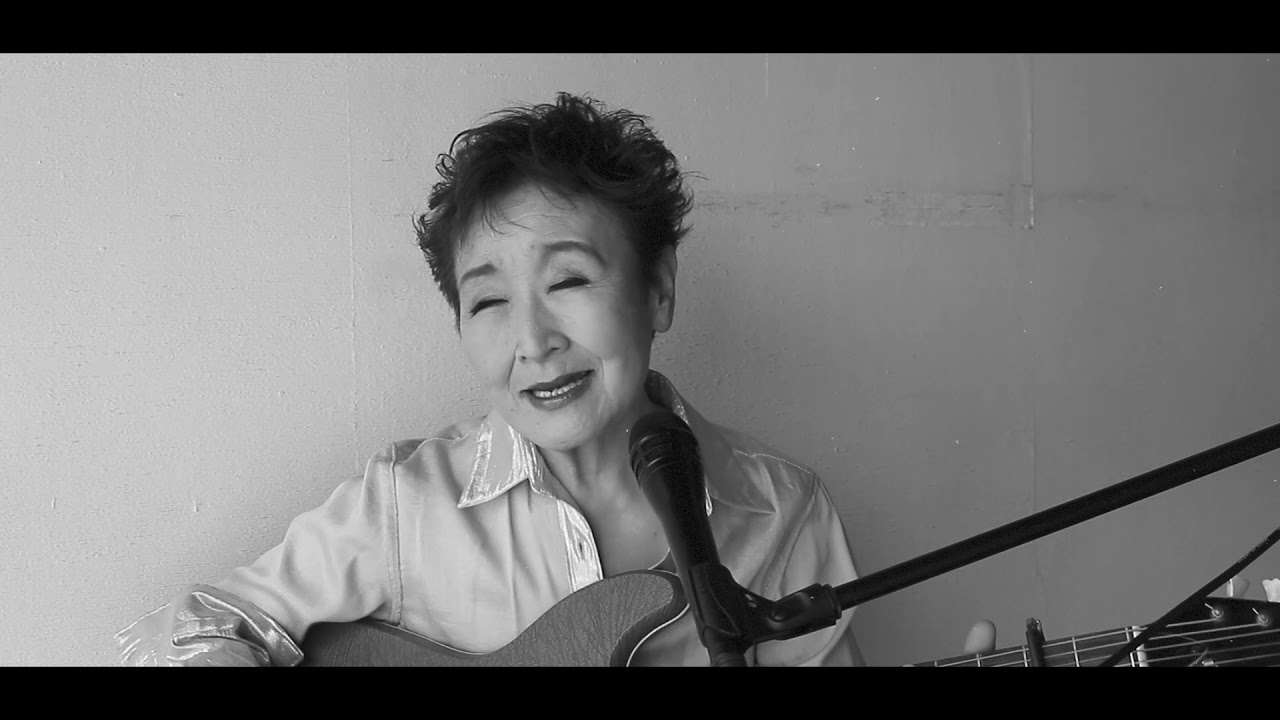
\includegraphics[width=0.48\linewidth]{pictures/youtube/2025/05/20250507_021435_youtube_001_Ny7W8D2CPEc.jpg}
}
\end{center}

\subsection*{2025年05月07日 02:15}
\addcontentsline{toc}{subsection}{2025年05月07日 02:15}

\paragraph{リンク}
\url{https://youtu.be/X3TTjKnGutk}

\begin{center}
\href{https://youtu.be/X3TTjKnGutk}{
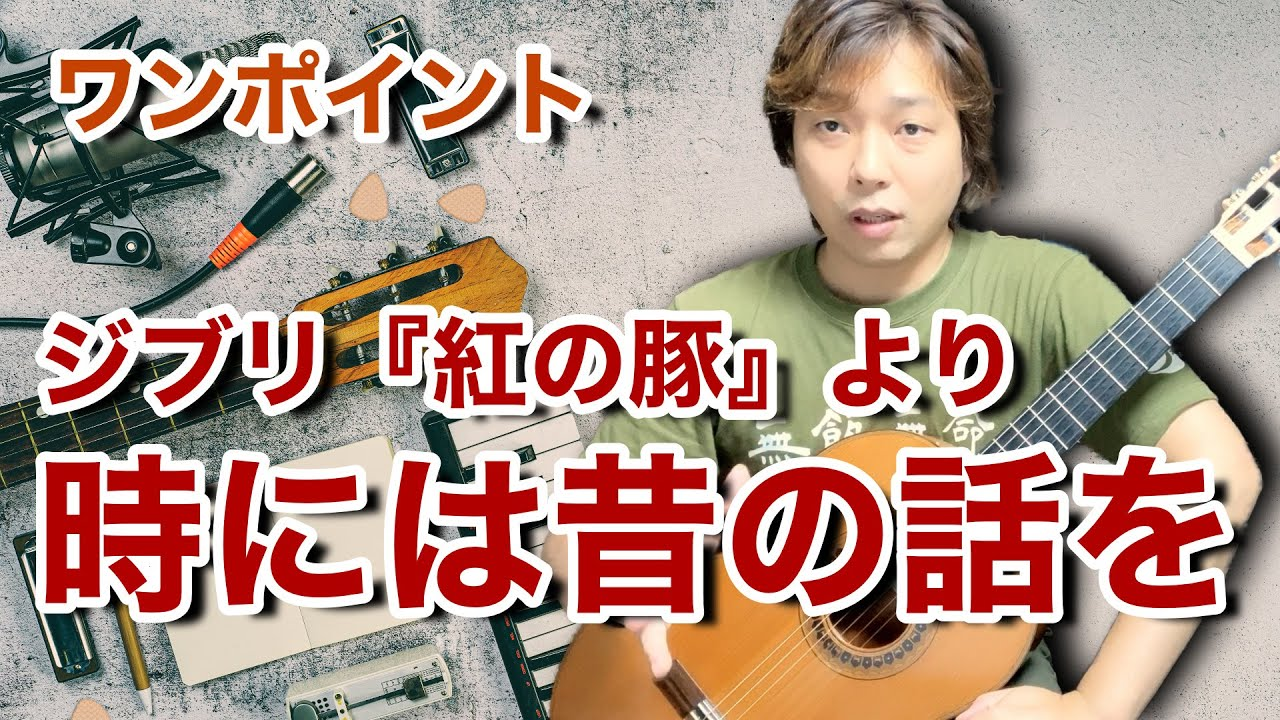
\includegraphics[width=0.48\linewidth]{pictures/youtube/2025/05/20250507_021555_youtube_001_X3TTjKnGutk.jpg}
}
\end{center}

\subsection*{2025年05月07日 03:01}
\addcontentsline{toc}{subsection}{2025年05月07日 03:01}

\paragraph{リンク}
\url{https://youtu.be/CmmHZ4cFaGg}

\begin{center}
\href{https://youtu.be/CmmHZ4cFaGg}{
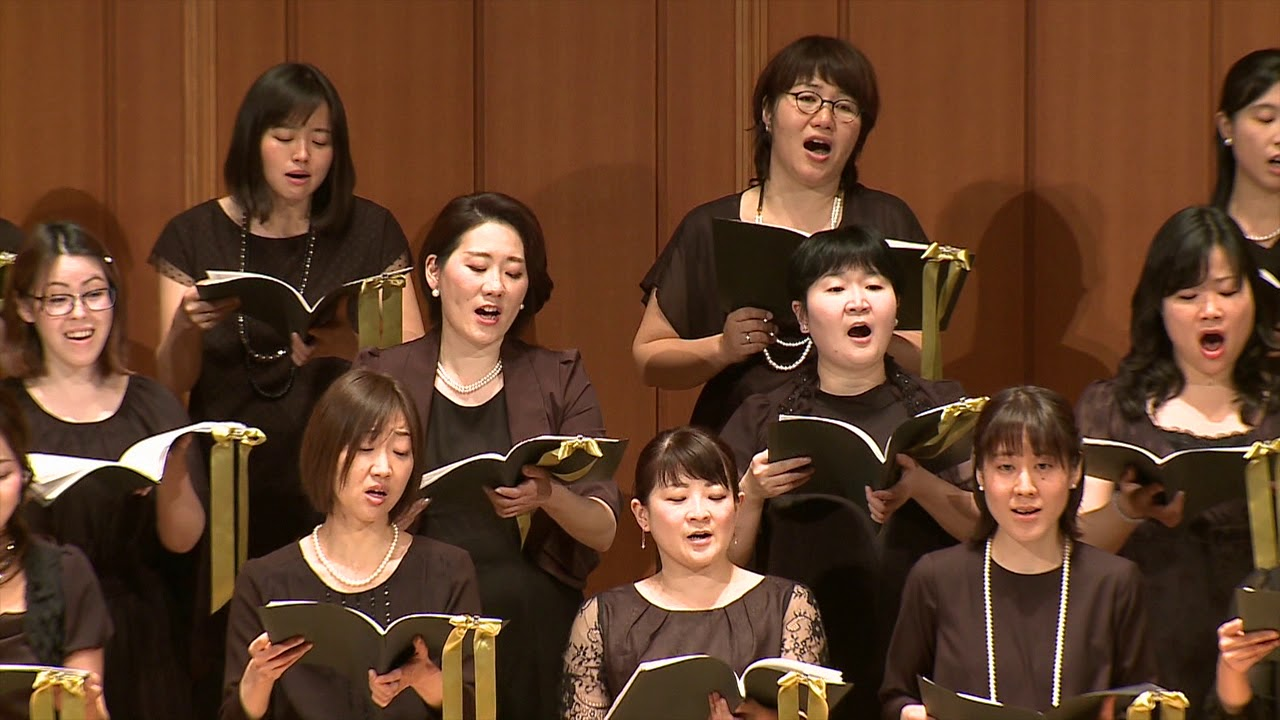
\includegraphics[width=0.48\linewidth]{pictures/youtube/2025/05/20250507_030126_youtube_001_CmmHZ4cFaGg.jpg}
}
\end{center}

\subsection*{2025年05月13日 10:13}
\addcontentsline{toc}{subsection}{2025年05月13日 10:13}

\url{https://youtu.be/kGXRsnU7jio}

\begin{center}
\href{https://youtu.be/kGXRsnU7jio}{
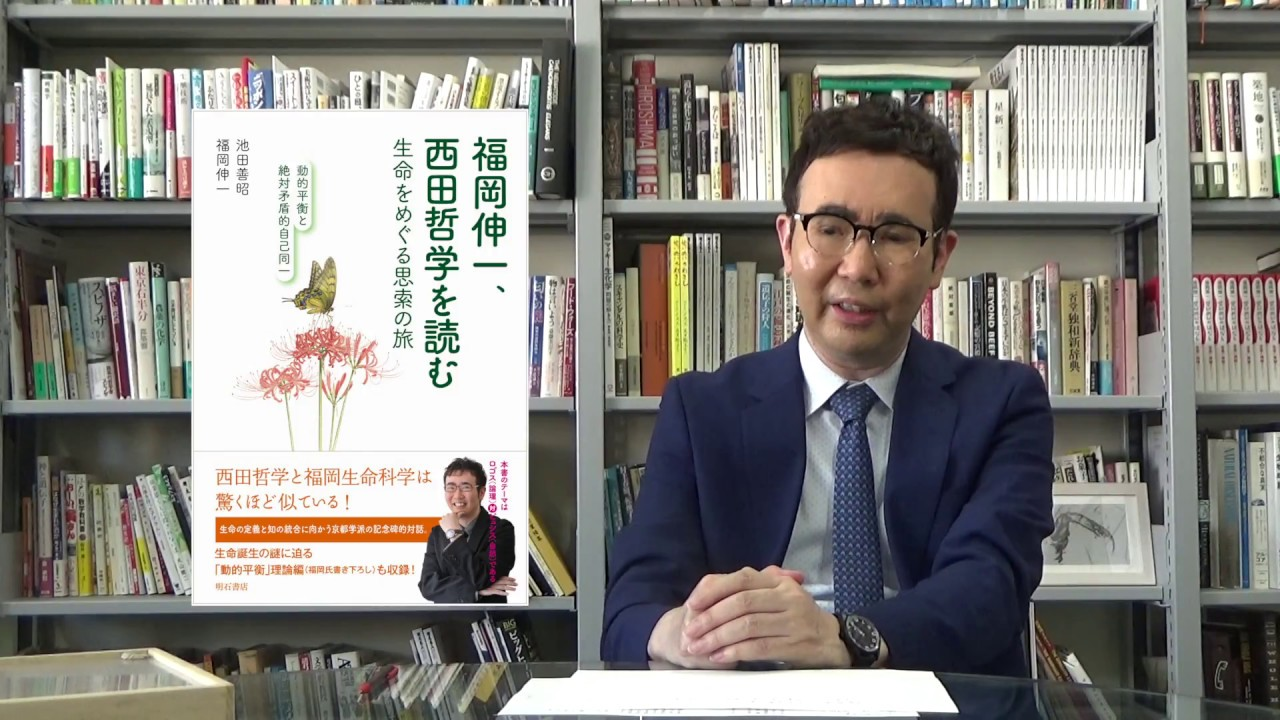
\includegraphics[width=0.48\linewidth]{pictures/youtube/2025/05/20250513_101350_youtube_001_kGXRsnU7jio.jpg}
}
\end{center}




この本は「 \#ロゴス の立ち位置からスタートして、\#ピュシス の視点に至ろうとするプロセス」が述べられているという事なのかもしれない、と思って読んでいくと、どうもそれがそもそも間違いだと言う事になる。ピュシスは直接「\#自覚」する必要がある（するもの「でなくてはならない 」）のだ、と。でも、先ずはロゴスの視点なら私でもある程度ついていけるかもしれない、と思って読み始めました。


\#福岡伸一 氏の「\#生物と無生物の間」は発売された当初に読みました。その本を書店で手にしたのは、帯に「\#生命とは何か」というキャッチコピーが書かれていたからです。この「生命とは何か」ですが、学生だった頃に \#岩波新書 から出ていた同じタイトルの本を読んだことがありました。


岩波新書の方の著者は \#シュレージンガー です。\#量子力学 の立役者として知られるシュレージンガーが物理だけでなく生物にも関わっていたのかと言う意外性がありました。そして更に、その本の主題が、\#熱力学の第二法則（\#エントロピー は増える＝「時間」の進む方向を規定している）に抗う様に、生命が維持存続できているのはなぜなのか、という問いでした。「本当だ、どうしてなんだろう」と不思議に思ったのが読み始めたきっかけです。この問いに対するシュレージンガーの答えは、壊れていくのを修復する、言わば「\#負のエントロピー」を食べているから、みたいな話だった様に記憶しています。ただし、負のエントロピーの実体が何なのか分からないまま終わっていましたし、そもそも熱力学の第二法則が言っていることは、エントロピーは正である、と言っている様に思えるものですから（エントロピーが負だと時間が逆行する）、かなり不満足な読後感だったと思います。（ただ、シュレージンガーの時代はまだ、DNAの二重螺旋構造も知られていなかった時代ですから、その問題意識そのものは流石です）


その後十年以上の月日が経って、福岡氏の「生物と無生物の間」に出会う事になります。この本でようやく「負のエントロピー」の正体が見えてきたという気になりました。それが福岡氏の言う「\#動的平衡」ではないのかと思ったのです。


\#西田幾多郎 哲学の「\#絶対矛盾的自己同一」とはどの様な概念なんでしょうか。また福岡氏の「動的平衡」が、西田幾多郎氏の「絶対矛盾的自己同一」とどう結びつくのでしょうか。これから楽しみに読み進めたいと思います。

\paragraph{写真}
\begin{center}
\begin{minipage}{0.48\linewidth}
\centering
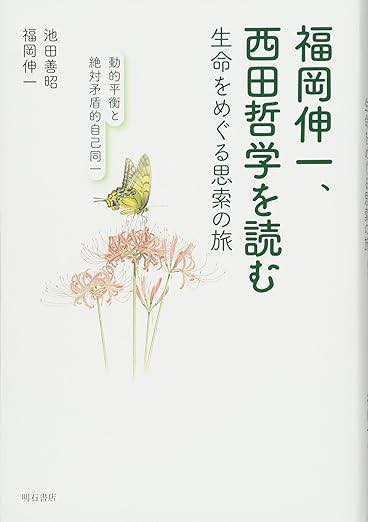
\includegraphics[width=\linewidth]{pictures/2025/05/20250513_101350_001.jpg}
\end{minipage}
\end{center}

\subsection*{2025年05月17日 07:19}
\addcontentsline{toc}{subsection}{2025年05月17日 07:19}

\url{https://youtu.be/hOTpama2I8Y}




\#理研 と \#富士通 が256 \#量子ビット のシャンデリアを開発したと報道されています。あるYouTube情報によるとQPUの温度は、10ミリ \#ケルビン 程だとか。ほぼ絶対零度に冷やされている超伝導状態です。温度がある→電磁波が出る→雑音になる←エラーの原因、という事だと記事には書かれていました。是非、日本がこの分野で世界をリードできる様になってほしいものです。


最近のネットの情報を見ていると、「文系だとか理系だ」とか、「量子力学って難しい」などと、「悠長な事」言ってる時代ではないという気がしてきます。QA4Uプロジェクトを見ていても、そんな気がします。\#線形代数 の「せ」の字、\#量子力学 の「り」の字も知らなくても、\#量子コンピュータ を使える＝量子コンピュータを使うアプリを書ける、そんな類いの人種がどうも沢山？いる（増えて来ている）様です。しかも年齢層の低いところ、高校生でも多数。インテグラル知らなくてもシグマ知ってればプログラムは書けるという事ですね。そう言えば、NANDもフリップフロップも知らなくても、外部記憶のファイルを操作するプログラムopen、read、write、close出来るからね。う〜ん、そうですね。そんな時代になって来ているという事なのでしょう。しかも、あっという間に！（控えめに言っても、そんな時代になりそうな「予感」がしてきています。）

\subsection*{2025年05月17日 15:03}
\addcontentsline{toc}{subsection}{2025年05月17日 15:03}

\paragraph{リンク}
\url{https://youtu.be/P88zPqMJ1kg}

\begin{center}
\href{https://youtu.be/P88zPqMJ1kg}{
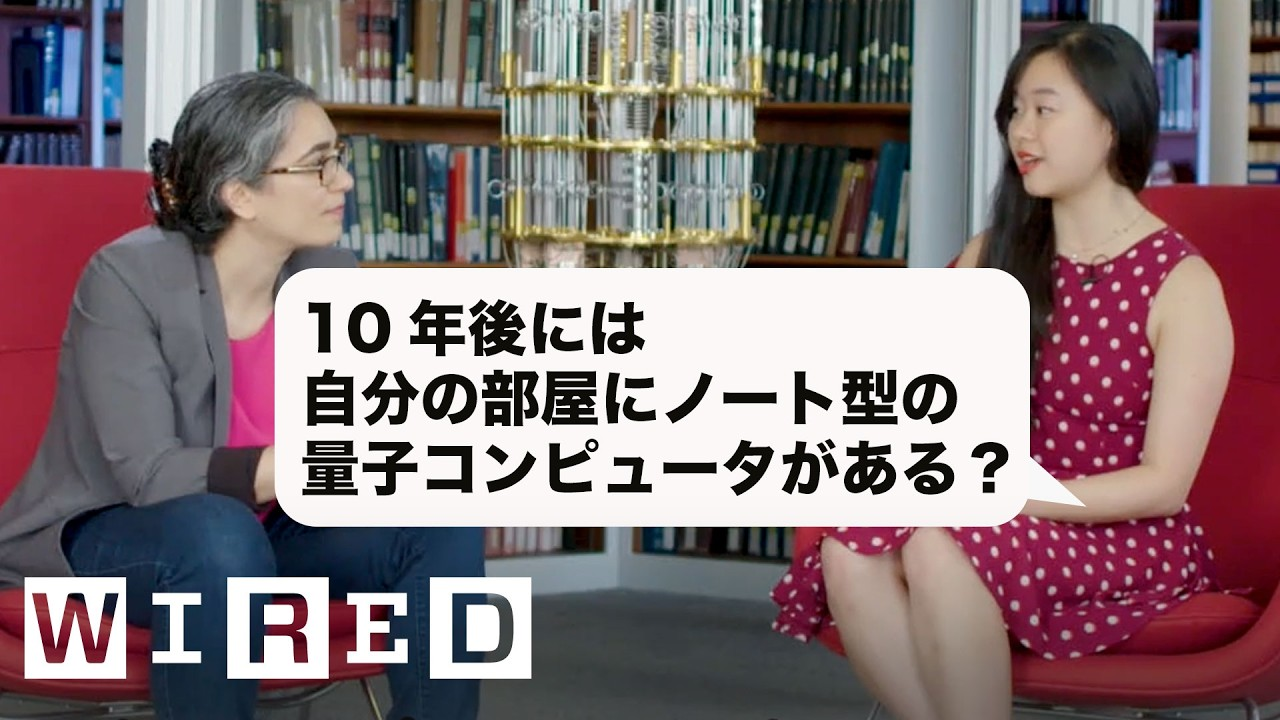
\includegraphics[width=0.48\linewidth]{pictures/youtube/2025/05/20250517_150315_youtube_001_P88zPqMJ1kg.jpg}
}
\end{center}

\subsection*{2025年05月18日 22:59}
\addcontentsline{toc}{subsection}{2025年05月18日 22:59}

\url{https://youtu.be/Q7sjDB1KFpE}

\begin{center}
\href{https://youtu.be/Q7sjDB1KFpE}{
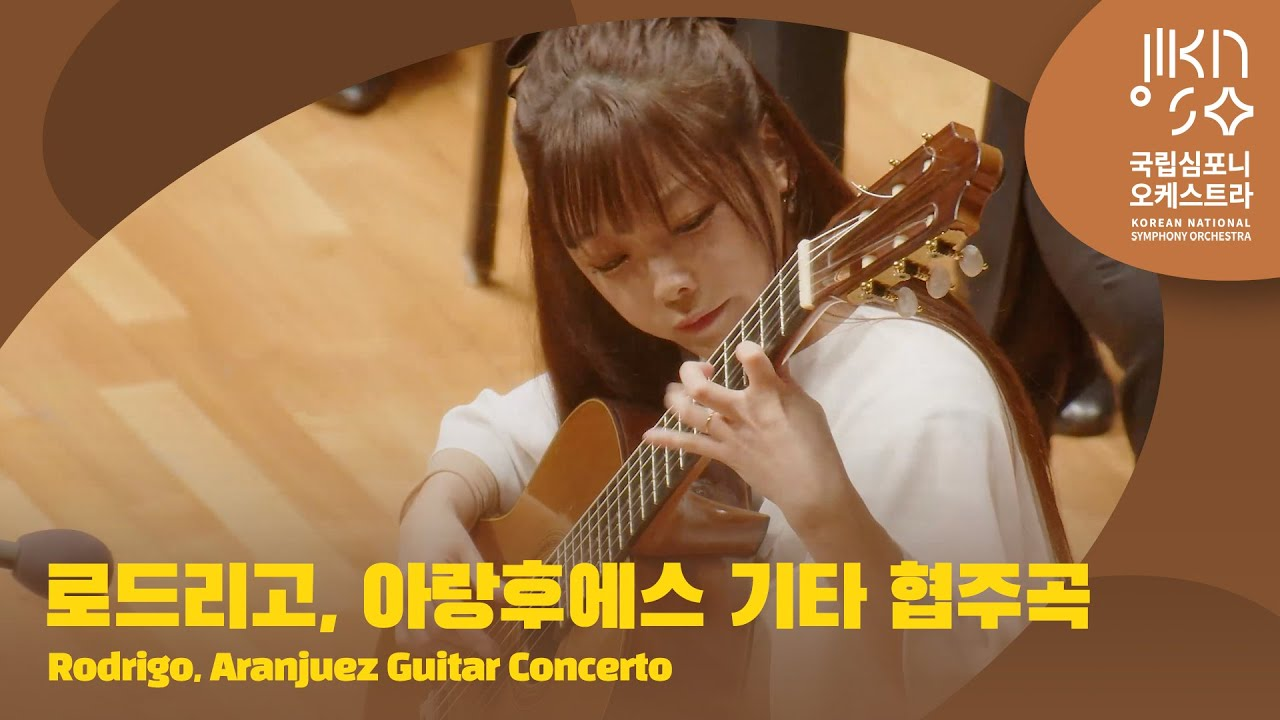
\includegraphics[width=0.48\linewidth]{pictures/youtube/2025/05/20250518_225957_youtube_001_Q7sjDB1KFpE.jpg}
}
\end{center}




やっぱりパク・キュヒ氏は凄いです。ほんまに凄い。

プロフェッショナルとは、皆んなそうなんでしょうか？(たまたま目に入ったのがキュヒ氏の演奏だったのでしょうか？）指を見ていると、特に高音部での運指や左手の指で弾くスラーやトリルなどが正確でごまかしの無い事、そしてギター一本でオケの全体との協奏が成っている事に「目が点」になってしまいます。ギターの表現力の多彩さにも今更ながら驚かされました。

この曲は、今まで真面に聞いたことはなかったのですが、正確な指の動き（演奏）に惹きつけられて、今回はじめて最後まで見て（聞いて）しまいました。


\#キュヒ \#ロドリーゴ \#アランフェス協奏曲

\subsection*{2025年05月19日 11:39}
\addcontentsline{toc}{subsection}{2025年05月19日 11:39}

\url{https://fb.watch/zGkLI02yJj/}




マーラーの六番。

「映画音楽か」と思っていた時期も個人的にはありましたが、（あらゆるプライドを捨てて素直に聞くと）やっぱりいいですね。グッときますよ。（バーンスタイン、こんなに髭はやしてることあったのか）


\#マーラー \#バーンスタイン

\subsection*{2025年05月20日 09:12}
\addcontentsline{toc}{subsection}{2025年05月20日 09:12}

\#金沢検定 対策のための IOS \#アプリ （\#Swift UIによる）を作ってみた。

表示させているデータのソースは、\#北國新聞社 から出ている「第19回金沢検定全問解説」です。


(１) データの入力はExcel（Numbers）等を使って入力する事にして、それを \#CSV に書き出したデータを、このアプリに読み込んで使います。

(２) 読み込んだデータは \#SQLite3 に入れて管理しているので、語句（キーワード）を使った前方一致、後方一致、任意一致などの検索も容易です。

(３) 答えと解説は通常は非表示ですが、選択肢から回答を選べば、表示される様にしています。（正解、不正解はチェックしていない。ブーとかピンポンとか鳴らなくても、答えが表示されるんだから正解だったかどうかは自分で見れば分かる。）

(４) また、四つの選択肢はその都度表示の順番を乱数で決めています。その問題が表示される度に、選択肢の表示順は異なる事になります。

(５) 左右へのフリック操作によって、次の問題、前の問題、ヘと移動する事ができます。


添付の画像は、

第「19」回金沢検定の「初」級の問題から、「史跡、、、建造物」の分野から出題された問題（全部で「15」問出題されていて、この問題はこの分野の中の「5」番目の問題）で、問題番号は初級全体通しで「40」番。その問題の四つの選択肢、解答と解説です。


アプリは、以前作った事のあった英単語暗記支援アプリ等から、切り出して組み直しているので、それ程時間をかけずにできてしまいました。


実はExcel（Numbers）への「データ入力の作業」そのものが、既に検定対策になってしまっています。CSVをアプリに読み込んで表示している段階では、データ入力作業を通して、内容はもう分かっているのですから。(じゃあ「アプリを作る意味は何？」と問い詰めてはいけません。単なる時間潰しなのですよ。)読んでいくと「へえ、そうだったのか」という様な驚きがあります。


プログラムのソースは、いつもの \#GitHub に置きました。

\url{https://github.com/smat1957/kanazawa_kentei}



CSVデータなどは一緒に置けません。（北國新聞社に忖度しています）


（その後）

検定対策と言っていましたが、アプリが完成してしまったら、知識としてはいつでも持ち歩けるものとなった（制覇した様な気になった）ので、検定を受けようという様な意欲はなくなりました。基本的に読み物として楽しむ事にしたいと思います。

\paragraph{写真}
\begin{center}
\begin{minipage}{0.48\linewidth}
\centering
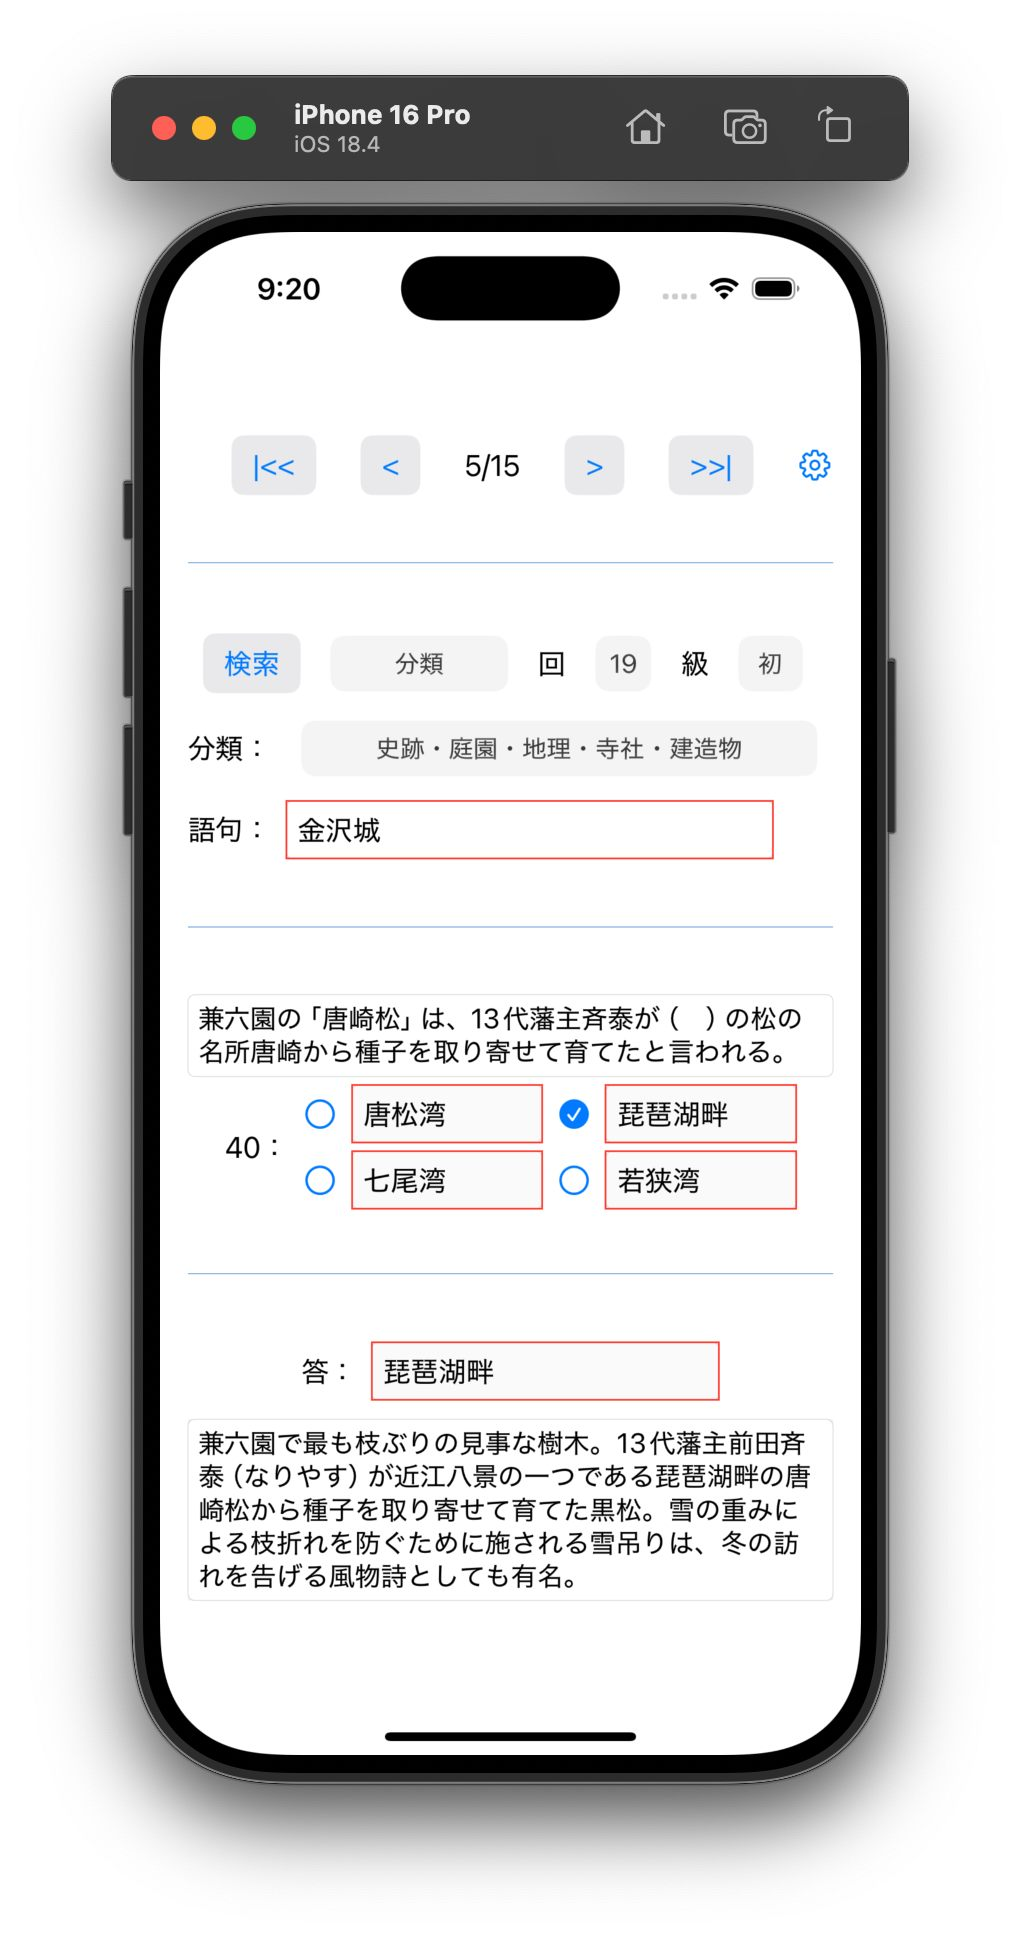
\includegraphics[width=\linewidth]{pictures/2025/05/20250520_091246_001.jpg}
\end{minipage}
\hfill
\begin{minipage}{0.48\linewidth}
\centering
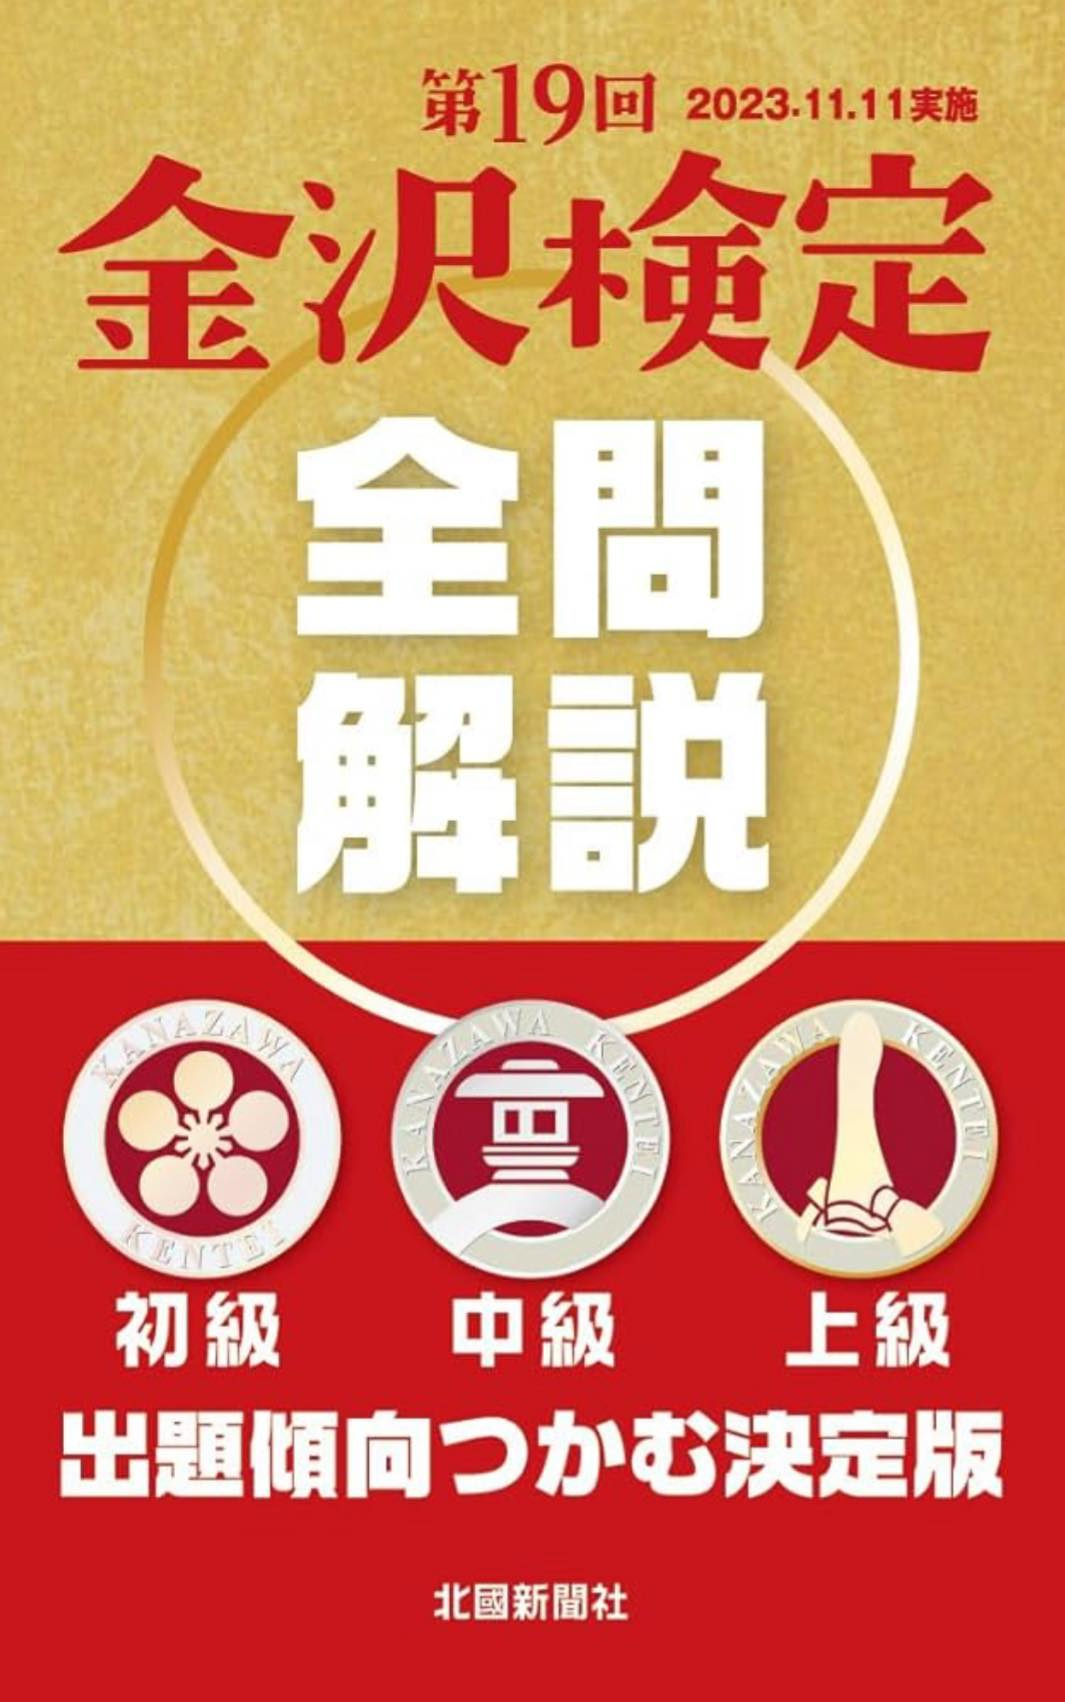
\includegraphics[width=\linewidth]{pictures/2025/05/20250520_091246_002.jpg}
\end{minipage}
\end{center}

\subsection*{2025年05月20日 22:58}
\addcontentsline{toc}{subsection}{2025年05月20日 22:58}

\paragraph{リンク}
\url{https://youtu.be/iPVtIP35VaA}

\begin{center}
\href{https://youtu.be/iPVtIP35VaA}{
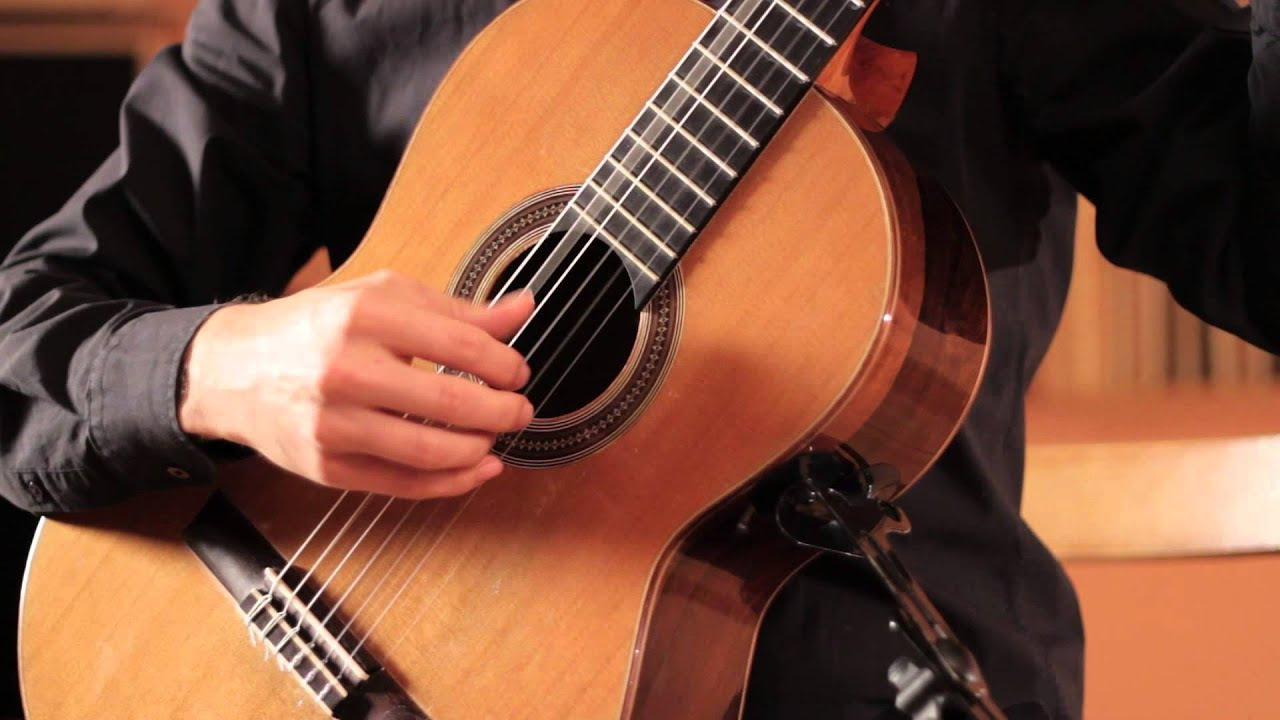
\includegraphics[width=0.48\linewidth]{pictures/youtube/2025/05/20250520_225802_youtube_001_iPVtIP35VaA.jpg}
}
\end{center}

\subsection*{2025年05月21日 02:48}
\addcontentsline{toc}{subsection}{2025年05月21日 02:48}

\paragraph{リンク}
\url{https://youtu.be/-lg0Y4sYATY}

\begin{center}
\href{https://youtu.be/-lg0Y4sYATY}{
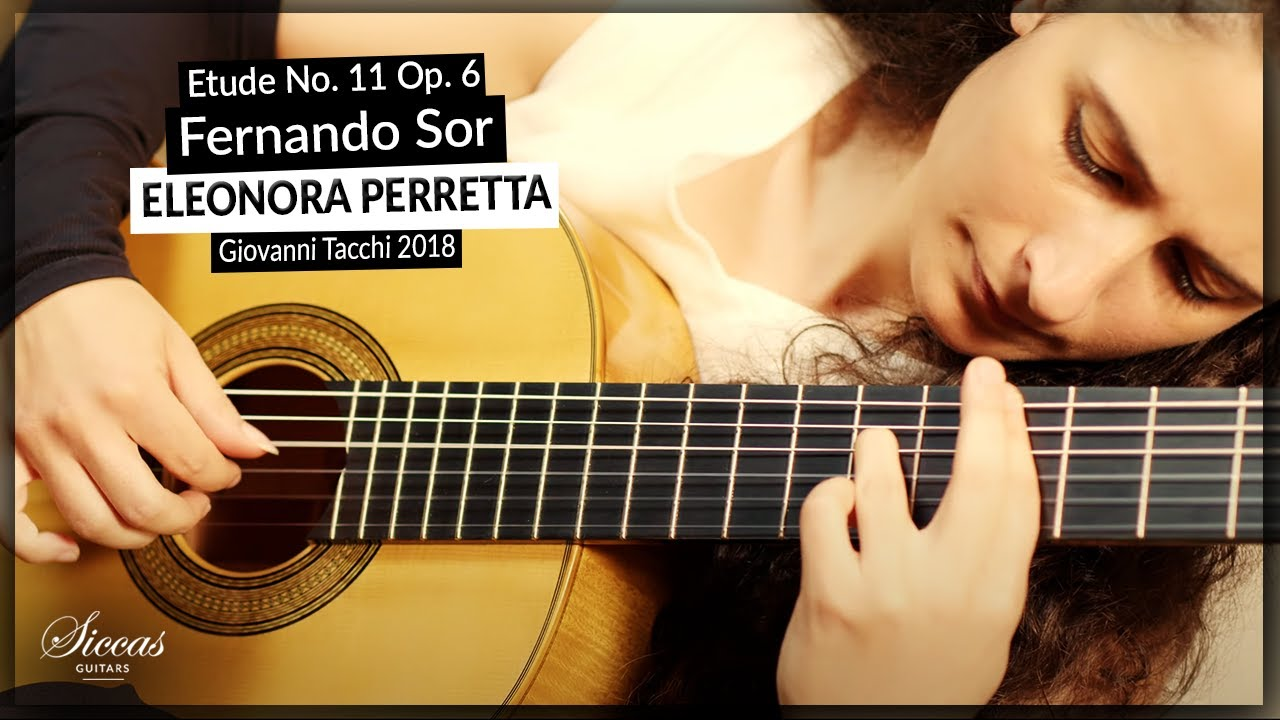
\includegraphics[width=0.48\linewidth]{pictures/youtube/2025/05/20250521_024851_youtube_001_-lg0Y4sYATY.jpg}
}
\end{center}

\subsection*{2025年05月21日 06:36}
\addcontentsline{toc}{subsection}{2025年05月21日 06:36}

\paragraph{リンク}
\url{https://youtu.be/yQCc7nQzUNo}

\begin{center}
\href{https://youtu.be/yQCc7nQzUNo}{
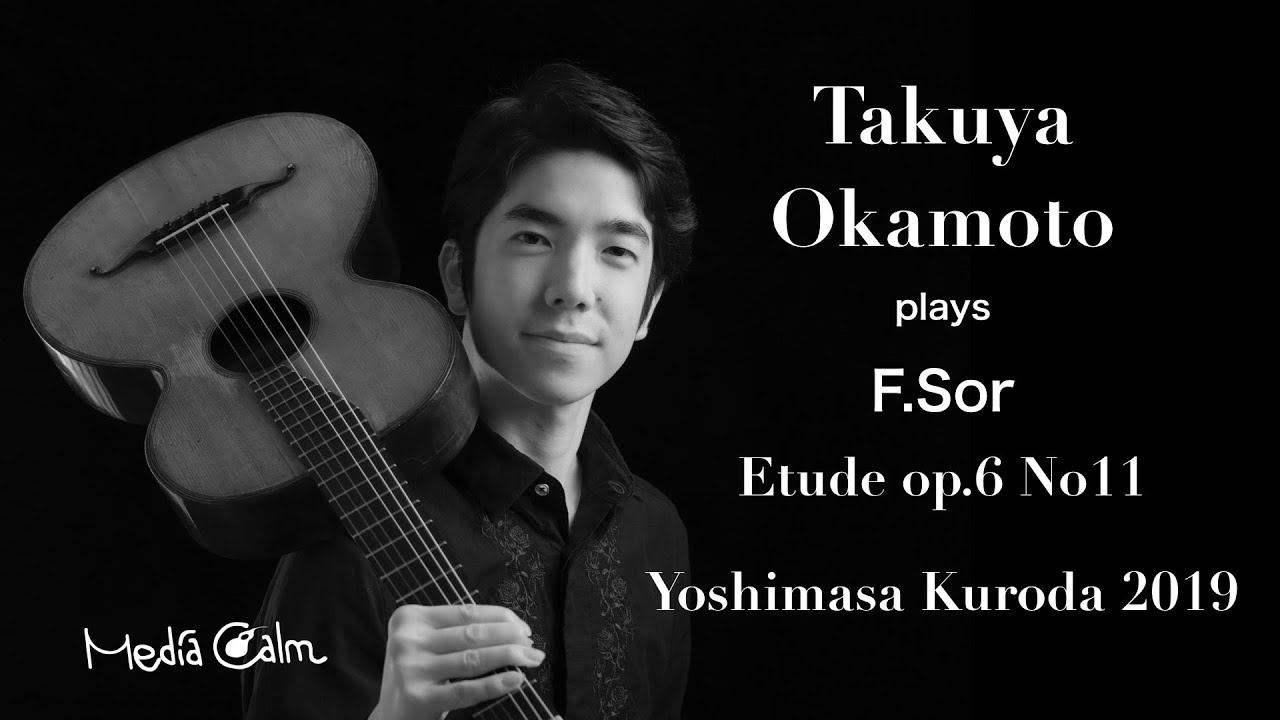
\includegraphics[width=0.48\linewidth]{pictures/youtube/2025/05/20250521_063622_youtube_001_yQCc7nQzUNo.jpg}
}
\end{center}

\subsection*{2025年05月24日 23:09}
\addcontentsline{toc}{subsection}{2025年05月24日 23:09}

石川県には、金沢市に \#鈴木大拙 館、かほく市に \#西田幾多郎 記念哲学館がある。それぞれの記念館に、何の予備知識もない状態で行ってみても何も得られないという気がした。そこで最近、この二人の思想に（先ずは、とにかく）触れてみようという気になっている。


これは、鈴木大拙氏のインタビュー番組です。

\url{https://youtu.be/EKtHvE5YoVU}

\begin{center}
\href{https://youtu.be/EKtHvE5YoVU}{
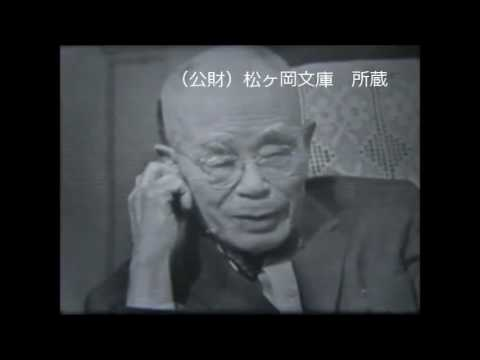
\includegraphics[width=0.48\linewidth]{pictures/youtube/2025/05/20250524_230917_youtube_001_EKtHvE5YoVU.jpg}
}
\end{center}



（ダイジェスト版になっている？ 

\url{https://youtu.be/3AKxPpfQs54}

 ）


instant=即今=ただ、今です。それだけが事実、本当です。それを人間の知恵で色々と分析して、時間というものをたてて、1分とか何億分の1とか言って、そこに未来や過去というものをこしらえる。無限の中ではそういうもの（未来や過去）はなくなる。そうすると、現在を生きるという事、今日限り、これ限り、今限りという「自覚」というか直覚というものがある、、、、


これを聞くと、鈴木大拙氏は西田幾多郎氏と同じ様な意味のことをおっしゃっているのではないかという気がする。（どちらもルーツは「禅」の思想なのか？）鈴木大拙氏の言う仏教の「分別視」とは、「ロゴス」の事ではないのか。「自覚」も西田哲学用語（？）にあったな。大拙氏が、「直覚」「そのまんま受け入れる、、」という様な話をされると、それは「ピュシス」かなと思う。「分かった様なわからん様な話」とは、西田氏であれば「絶対矛盾的自己同一」とおっしゃるかもしれません。


（西田氏と大拙氏が似た様な事をおっしゃっているという気がしたというだけの話であって、私がその話の内容を理解したというわけでは決してない。そもそも私は両氏の極ゞ一断面をちょっとだけ垣間見たに過ぎないのですから。入門書として良いのではないかと思い、添付画像の本も手にしてみています。）

\paragraph{写真}
\begin{center}
\begin{minipage}{0.48\linewidth}
\centering
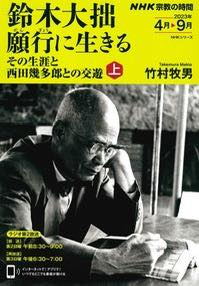
\includegraphics[width=\linewidth]{pictures/2025/05/20250524_230917_001.jpg}
\end{minipage}
\hfill
\begin{minipage}{0.48\linewidth}
\centering
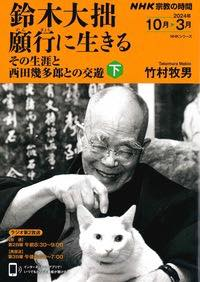
\includegraphics[width=\linewidth]{pictures/2025/05/20250524_230917_002.jpg}
\end{minipage}
\end{center}

\begin{center}
\begin{minipage}{0.48\linewidth}
\centering
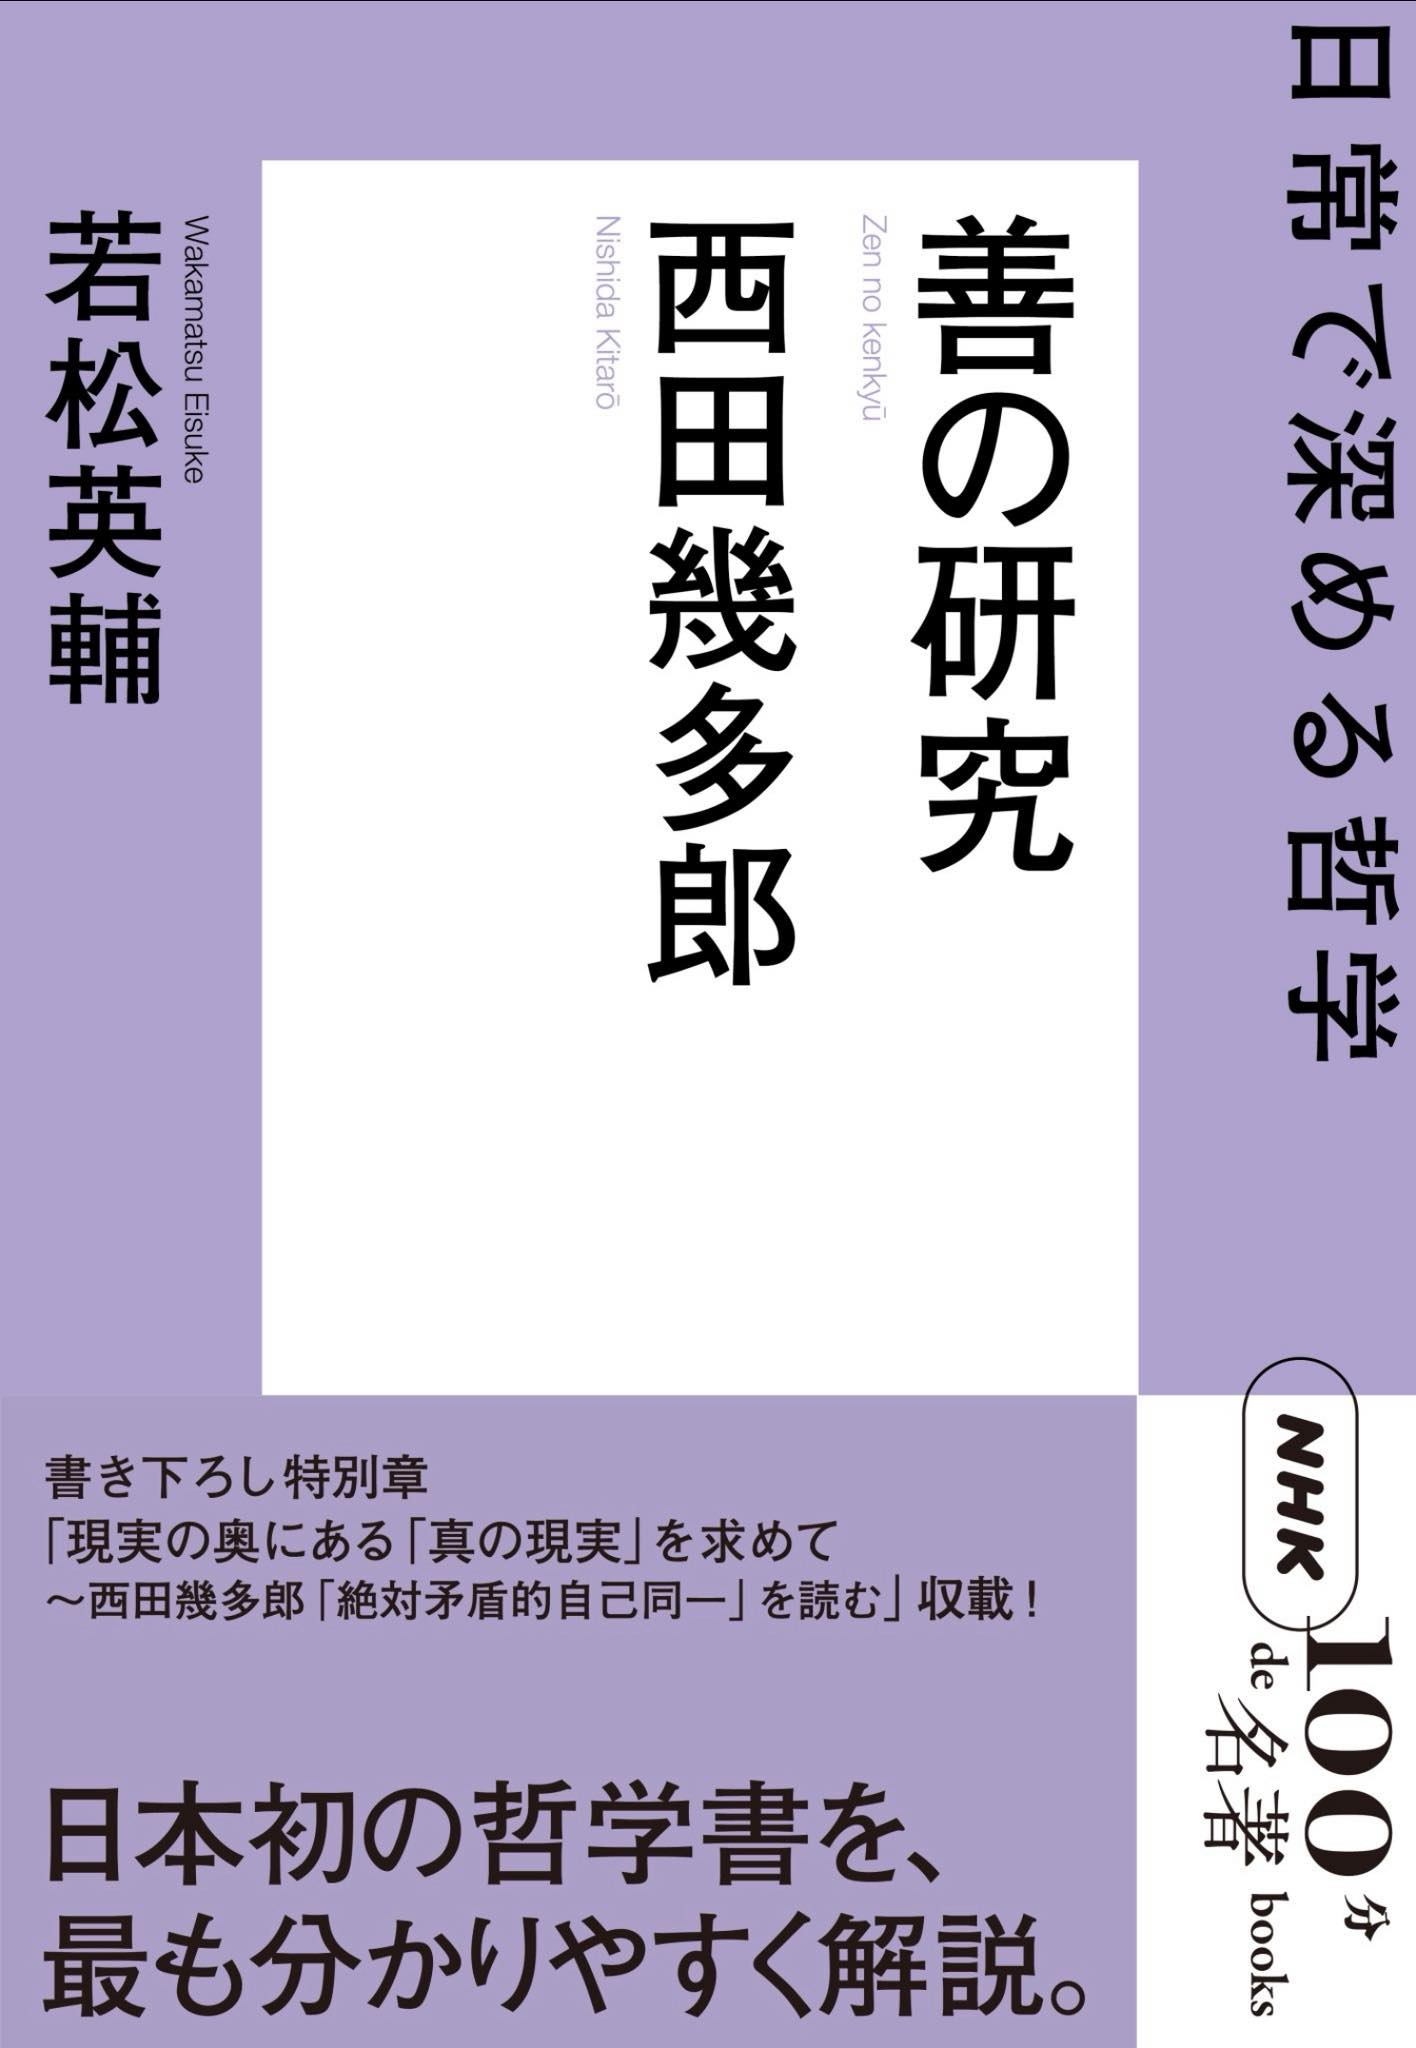
\includegraphics[width=\linewidth]{pictures/2025/05/20250524_230917_003.jpg}
\end{minipage}
\hfill
\begin{minipage}{0.48\linewidth}
\centering
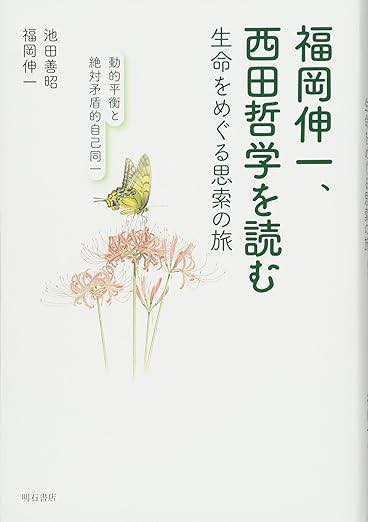
\includegraphics[width=\linewidth]{pictures/2025/05/20250524_230917_004.jpg}
\end{minipage}
\end{center}

\subsection*{2025年05月28日 18:00}
\addcontentsline{toc}{subsection}{2025年05月28日 18:00}

緑いっぱいの \#哲学の道 を歩き（「探検」し）ました。


この道のスタート位置は（ \#銀閣寺 参道からの入り口ではなくて） \#今出川通 りと \#白川通 りが交叉する \#浄土寺橋 。終わりは、\#熊野若王子神社 （近くに \#新島襄 と \#八重 の墓があるらしい）の前の \#若王子橋 です。本来は \#琵琶湖疏水 の管理用道路で、距離は約2kmほどあるとの事です。


この道には、\#西田幾多郎 氏の筆跡による句碑が置かれています。でも、観光客は誰も振り返らずに（気づかないまま）通り過ぎている様でした。（この日、ここの観光客に日本人は稀でした。外人さんは碑に彫られた文字が分からない可能性大ですし。）


「人は人 吾はわれ也 とにかくに 吾行く道を 吾は行くなり」


この（力強い）句を読んで、決意を新たにする若者も（少なからず）いたかもしれません。（或いは西田氏も、理解されない、などと悩んだりする事、あっただろうか？）


途中、\#法然院 に立ち寄るつもりでしたが、\#法然院橋 （西田幾多郎の句碑のある所の橋より、一つ銀閣寺寄りの橋）を渡って、登り道をつき当たりまで行き、そこを右折、その後「左折する道を見逃した」みたいです。真っ直ぐに進んでしまって、どうやら \#安楽寺 に向かっていた様でした。（同じ道を行ったり来たりしたので、iPhoneに記録された移動距離は長くなりました。）


なお、今回初めて知った事なのですが、\#若王子 は、「にゃく」おうじ、と読む様です。

\paragraph{写真}
\begin{center}
\begin{minipage}{0.48\linewidth}
\centering
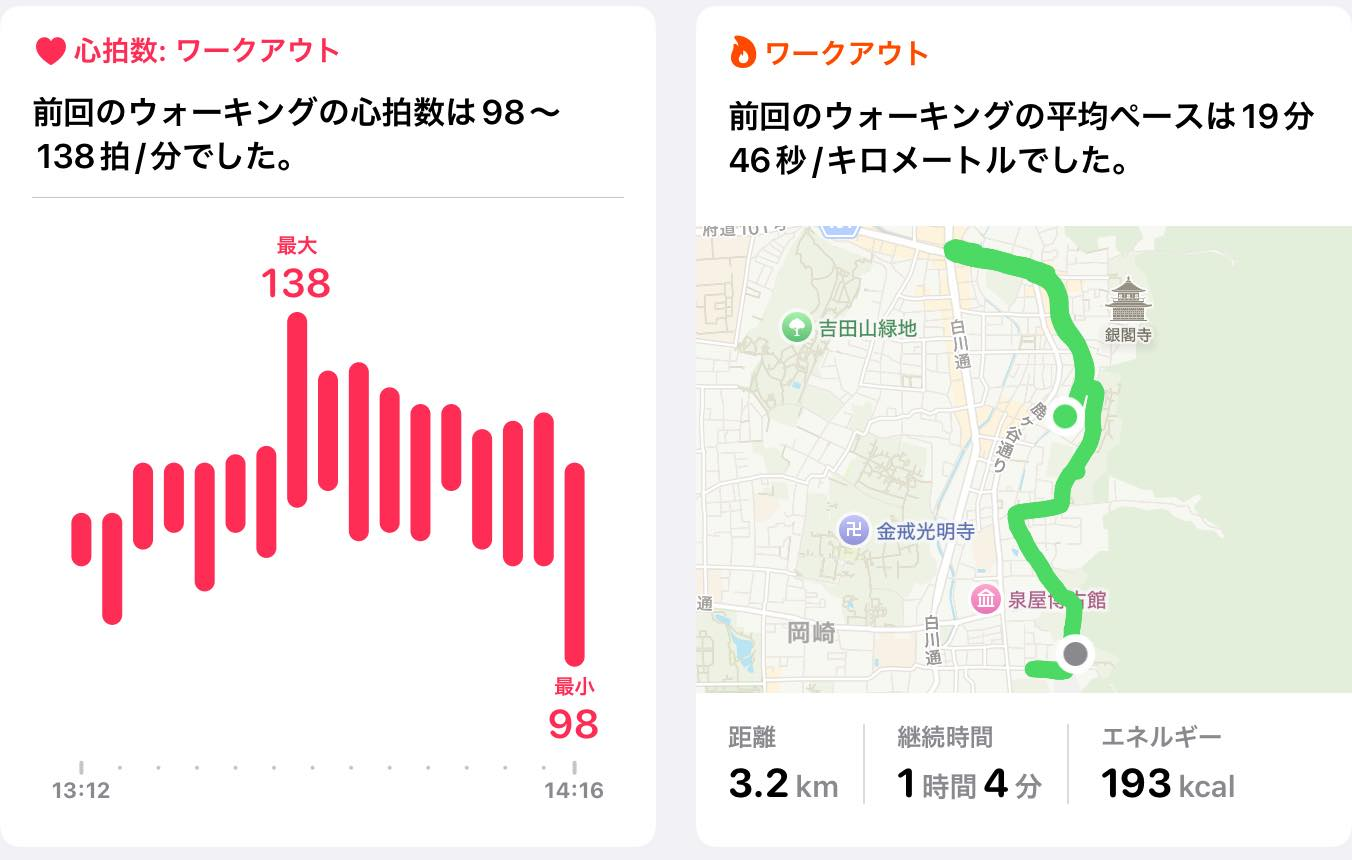
\includegraphics[width=\linewidth]{pictures/2025/05/20250528_180009_001.jpg}
\end{minipage}
\hfill
\begin{minipage}{0.48\linewidth}
\centering
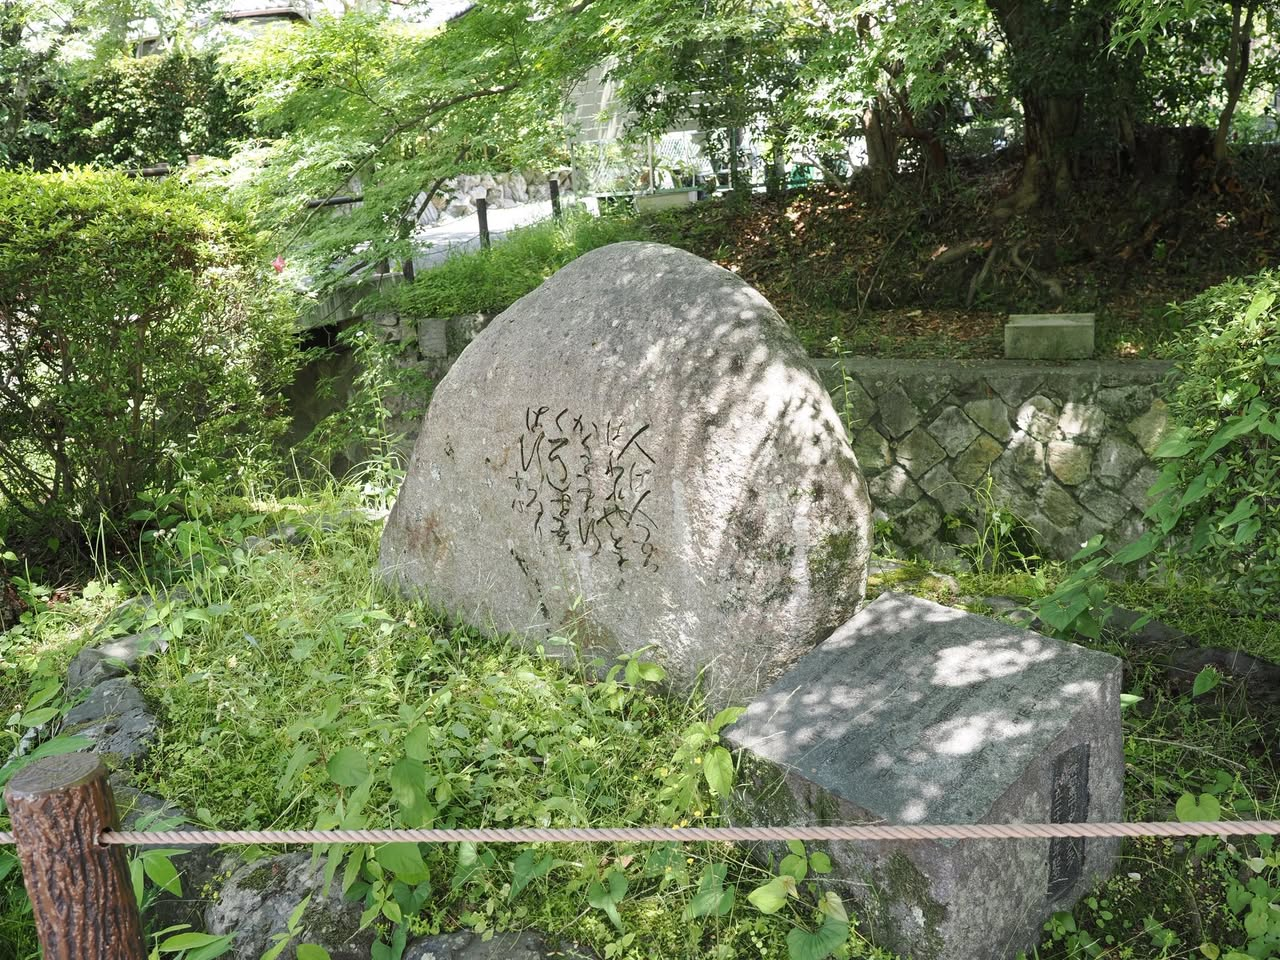
\includegraphics[width=\linewidth]{pictures/2025/05/20250528_180009_002.jpg}
\end{minipage}
\end{center}

\subsection*{2025年05月30日 11:33}
\addcontentsline{toc}{subsection}{2025年05月30日 11:33}

\paragraph{リンク}
\url{https://youtu.be/WIoFVHJYiYw}

\begin{center}
\href{https://youtu.be/WIoFVHJYiYw}{
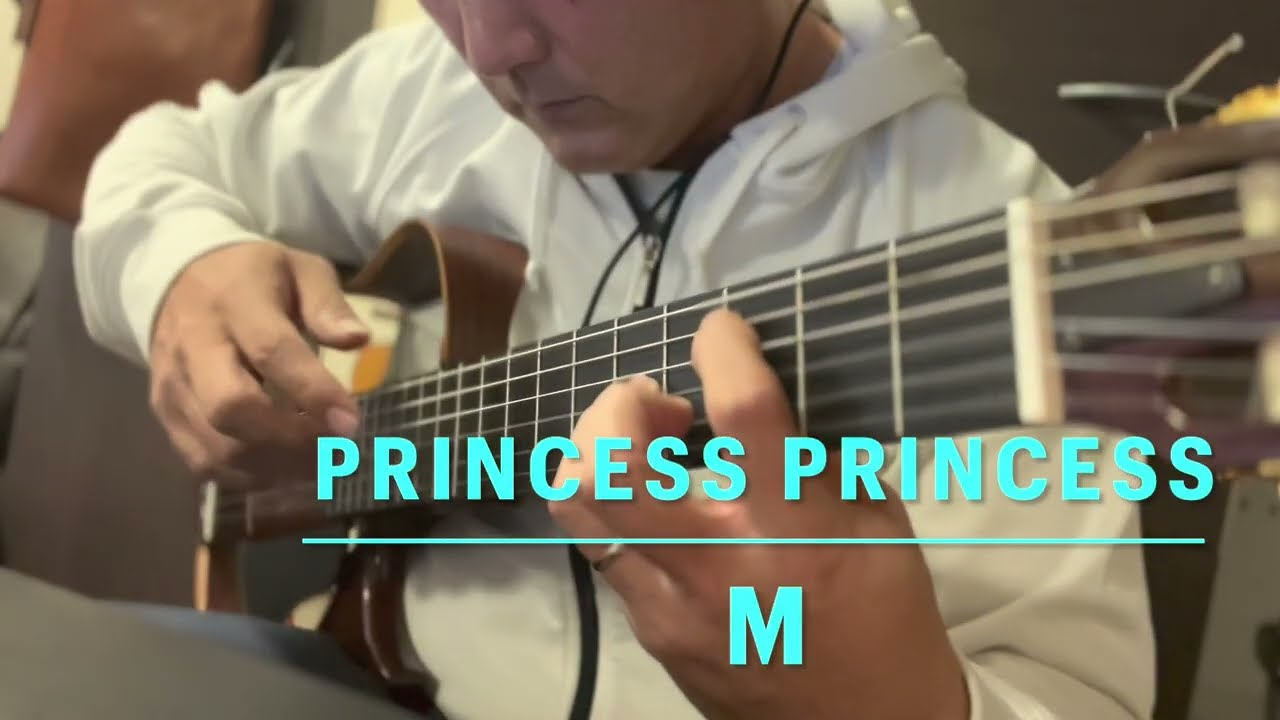
\includegraphics[width=0.48\linewidth]{pictures/youtube/2025/05/20250530_113302_youtube_001_WIoFVHJYiYw.jpg}
}
\end{center}

\subsection*{2025年05月30日 21:11}
\addcontentsline{toc}{subsection}{2025年05月30日 21:11}

「ソルの20の練習曲」ですが、セゴビア「編」と、セゴビア「選」の両方が存在している様です。セゴビア「選」は、単にセゴビアが選んだ20曲を集めた曲集ですと言う意味。セゴビアが編集して表情を付け運指を決めたりしたセゴビア「編」とは別ものでした。


現在、日本でセゴビア「編」は出版されていません。海外で出版されているセゴビア「編」の楽譜は、輸入される度に売り切れ御免となるので、入手がちょっと面倒そうな様相です。（学生の頃は日本でも出版されていたので、「編」を持っていたんだけど、どこに行っちゃったことか、分からない）


セゴビア「選」なら普通に購入できます。（昔弾いてみていたのと、ちょっと違うぞと思ったら、案の定「選」でした。）「選」の表紙には「オリジナル版」と言う記述がありますが、これは「セゴビア編」などの様に後世の人が編纂した楽譜ではなくて、ソルが書いた楽譜そのままですよ、という意味？なのかな。

\paragraph{写真}
\begin{center}
\begin{minipage}{0.48\linewidth}
\centering
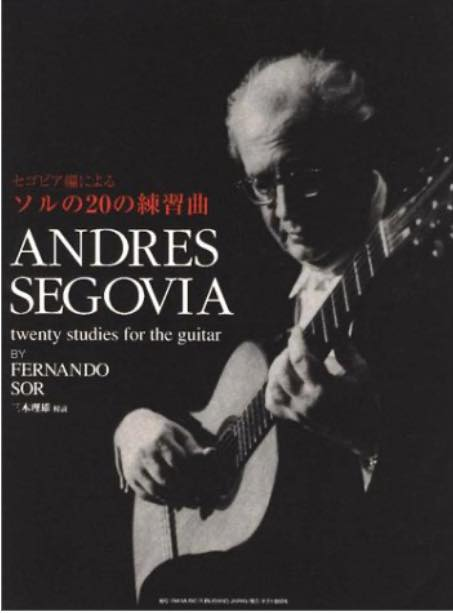
\includegraphics[width=\linewidth]{pictures/2025/05/20250530_211112_001.jpg}
\end{minipage}
\hfill
\begin{minipage}{0.48\linewidth}
\centering
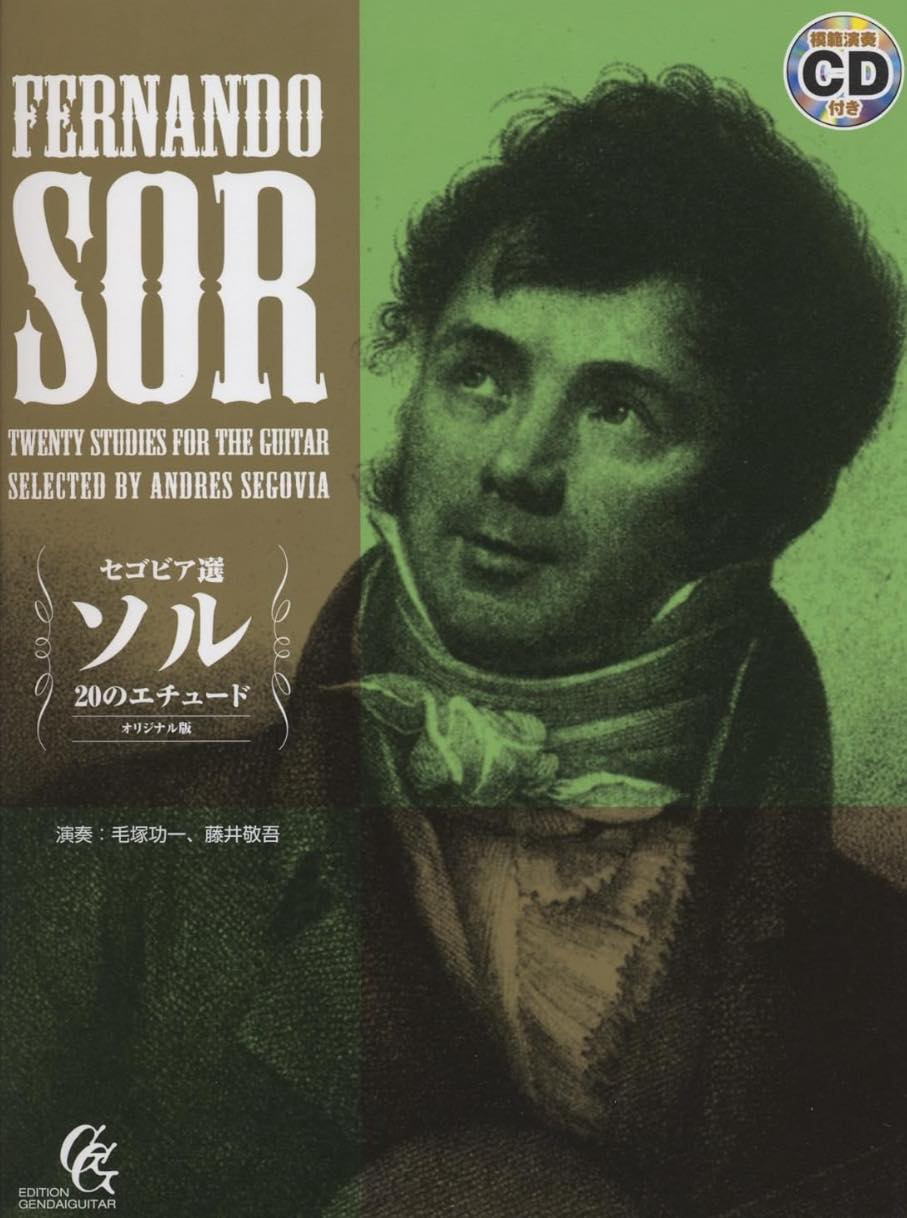
\includegraphics[width=\linewidth]{pictures/2025/05/20250530_211112_002.jpg}
\end{minipage}
\end{center}

\section{6月}

\subsection*{2025年06月01日 19:33}
\addcontentsline{toc}{subsection}{2025年06月01日 19:33}

\paragraph{リンク}
\url{https://youtu.be/dO2E9mqou1g}

\begin{center}
\href{https://youtu.be/dO2E9mqou1g}{
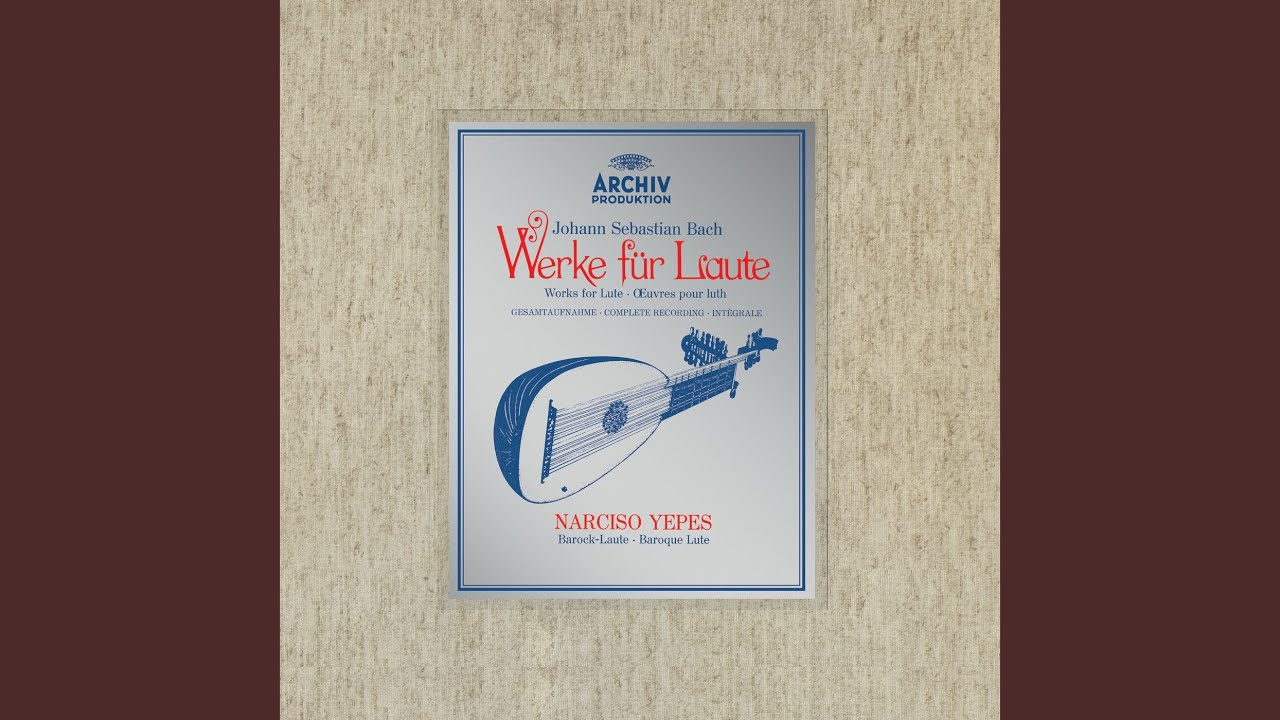
\includegraphics[width=0.48\linewidth]{pictures/youtube/2025/06/20250601_193345_youtube_001_dO2E9mqou1g.jpg}
}
\end{center}

\subsection*{2025年06月02日 07:01}
\addcontentsline{toc}{subsection}{2025年06月02日 07:01}

\paragraph{リンク}
\url{https://youtu.be/d3Vj_mfJmcg}

\begin{center}
\href{https://youtu.be/d3Vj_mfJmcg}{
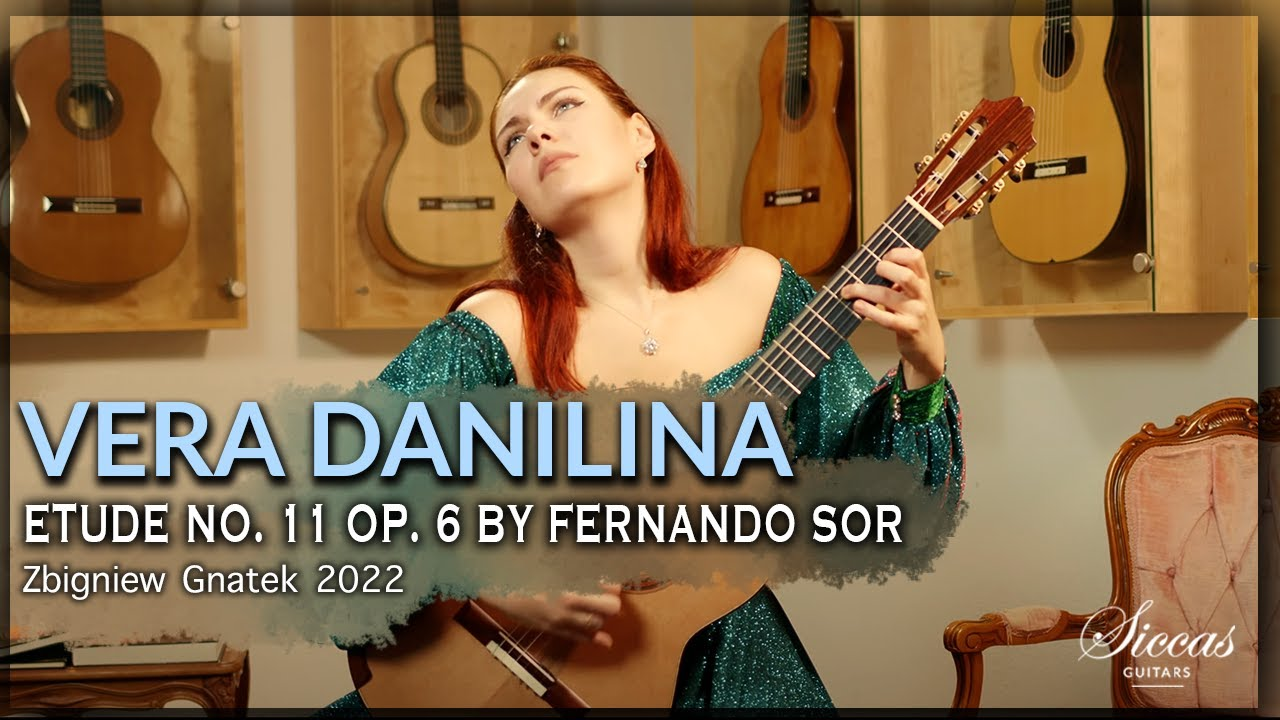
\includegraphics[width=0.48\linewidth]{pictures/youtube/2025/06/20250602_070158_youtube_001_d3Vj_mfJmcg.jpg}
}
\end{center}

\subsection*{2025年06月02日 07:04}
\addcontentsline{toc}{subsection}{2025年06月02日 07:04}

\paragraph{リンク}
\url{https://youtu.be/IEw_p72Uwe8}

\begin{center}
\href{https://youtu.be/IEw_p72Uwe8}{
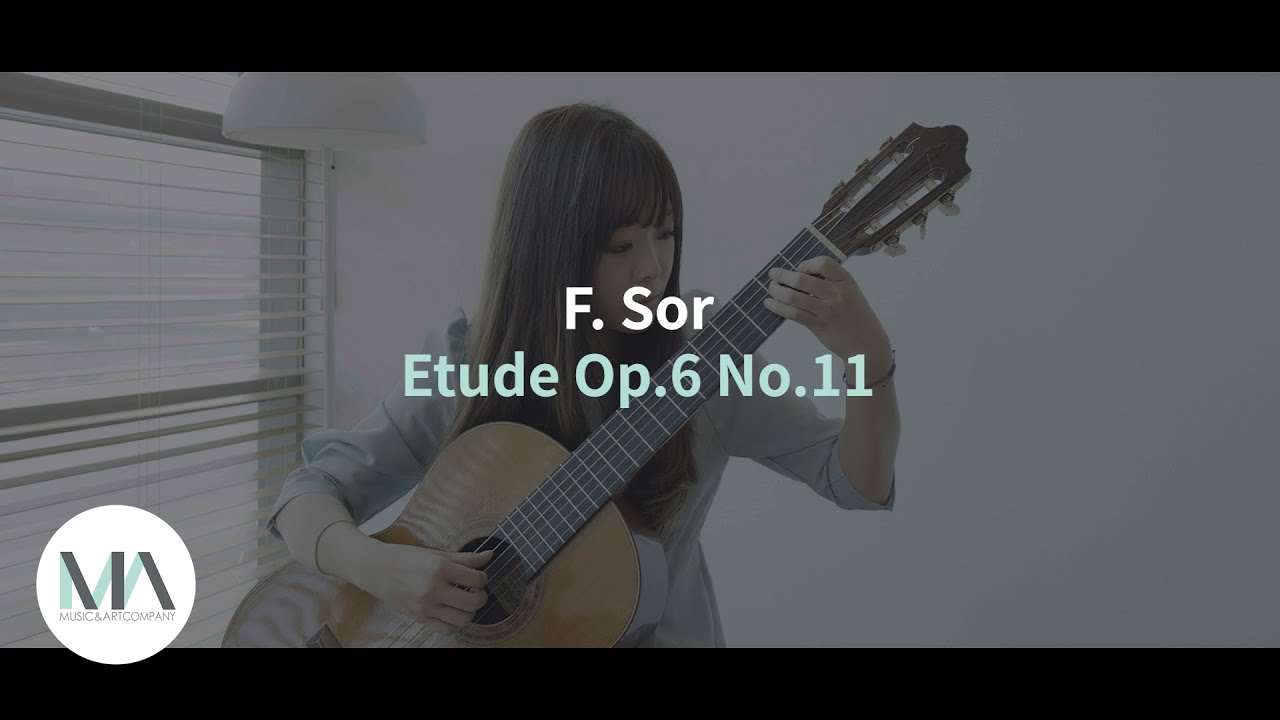
\includegraphics[width=0.48\linewidth]{pictures/youtube/2025/06/20250602_070425_youtube_001_IEw_p72Uwe8.jpg}
}
\end{center}

\subsection*{2025年06月03日 09:20}
\addcontentsline{toc}{subsection}{2025年06月03日 09:20}

\paragraph{リンク}
\url{https://youtu.be/2UA23gXP5ok}

\begin{center}
\href{https://youtu.be/2UA23gXP5ok}{
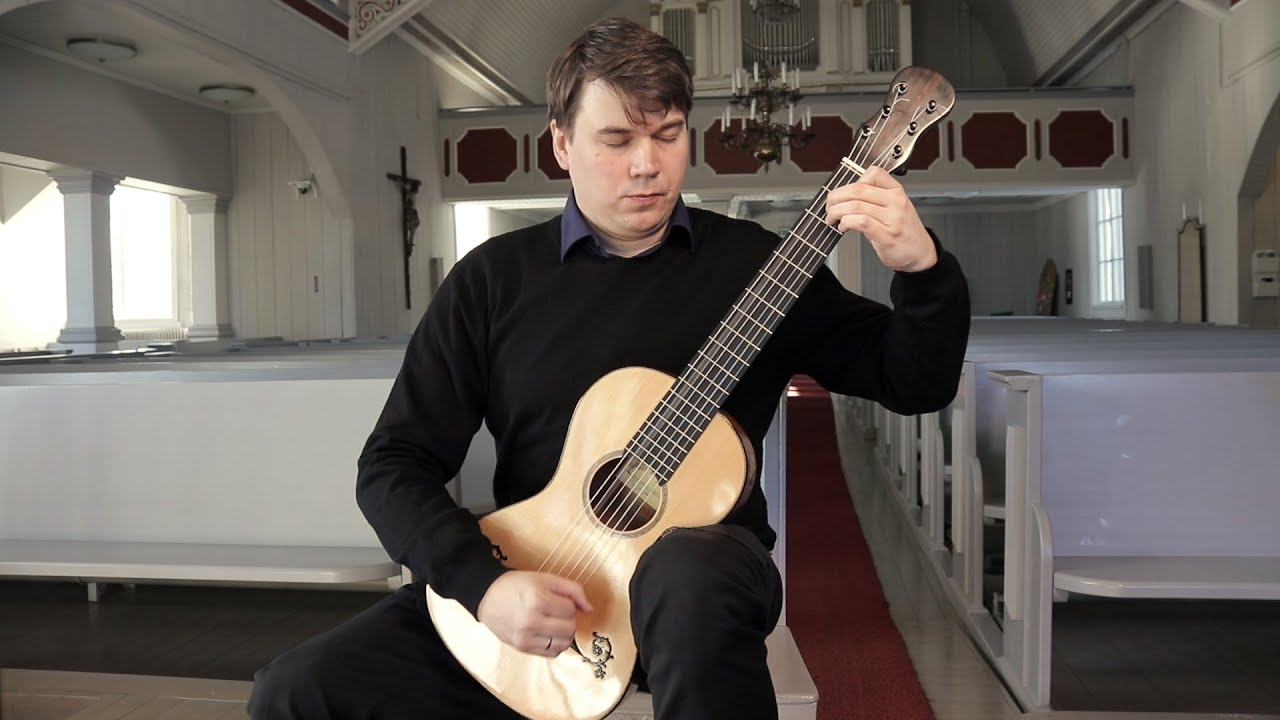
\includegraphics[width=0.48\linewidth]{pictures/youtube/2025/06/20250603_092018_youtube_001_2UA23gXP5ok.jpg}
}
\end{center}

\subsection*{2025年06月03日 22:05}
\addcontentsline{toc}{subsection}{2025年06月03日 22:05}

「主よあわれみ給え」エルバルメ ディッヒ

\url{https://youtu.be/of-WOH-uxYs}

\begin{center}
\href{https://youtu.be/of-WOH-uxYs}{
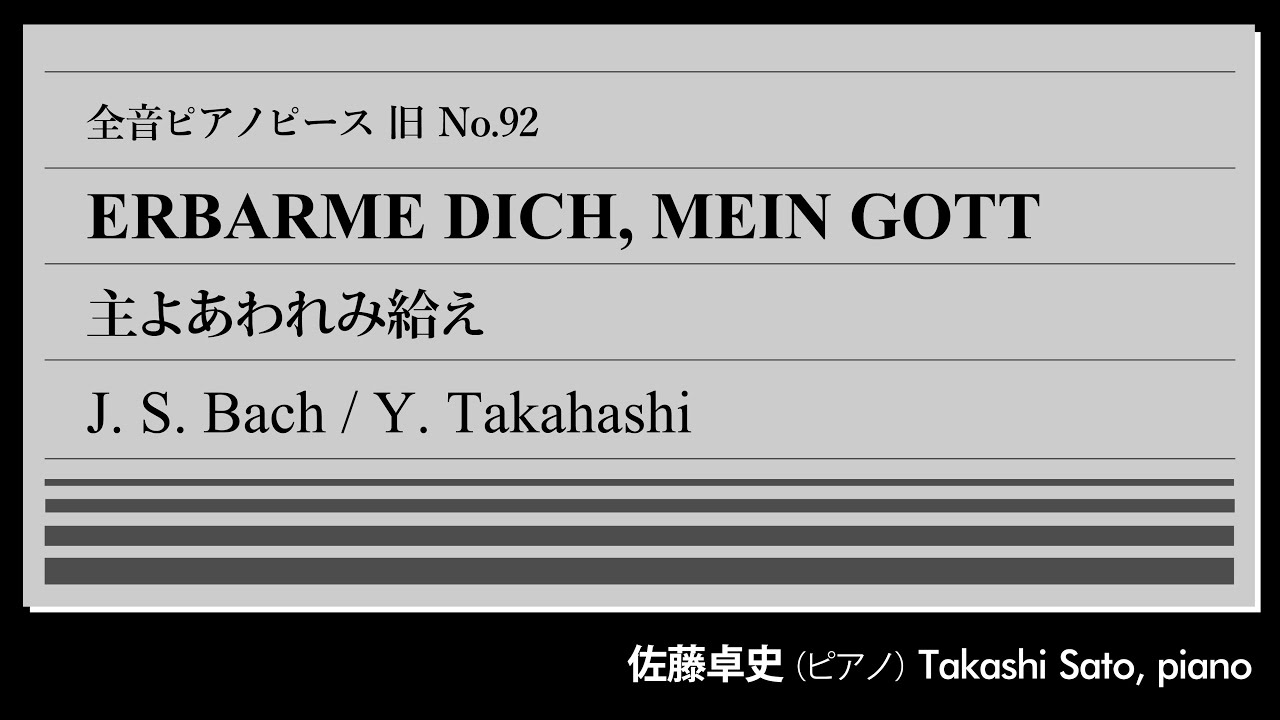
\includegraphics[width=0.48\linewidth]{pictures/youtube/2025/06/20250603_220510_youtube_001_of-WOH-uxYs.jpg}
}
\end{center}



途中から、かなり複雑な（高橋悠治氏らしい）編曲になっている様です


高橋悠治氏の公式サイト

\url{https://suigyu.com/yuji_takahashi/}



ここに楽譜のPDFが公開されている


マタイ受難曲を全部聞こうと思ったら、例えば次のリンクがある。一応カールリヒターは定番とされていますが（どうなんでしょうか？）私は、アムステルダム  ロイヤル コンセルトヘボウ をイヴァン フィッシャーがふっているブルーレイが気に入って聞いています。ただ、古楽器による演奏で何かいいのないかな？とは、いつも気にしています（BCJなのかな）


カールリヒター、マタイ受難曲　← 定番

\url{https://youtu.be/v0lMWnBzUkY}

\begin{center}
\href{https://youtu.be/v0lMWnBzUkY}{
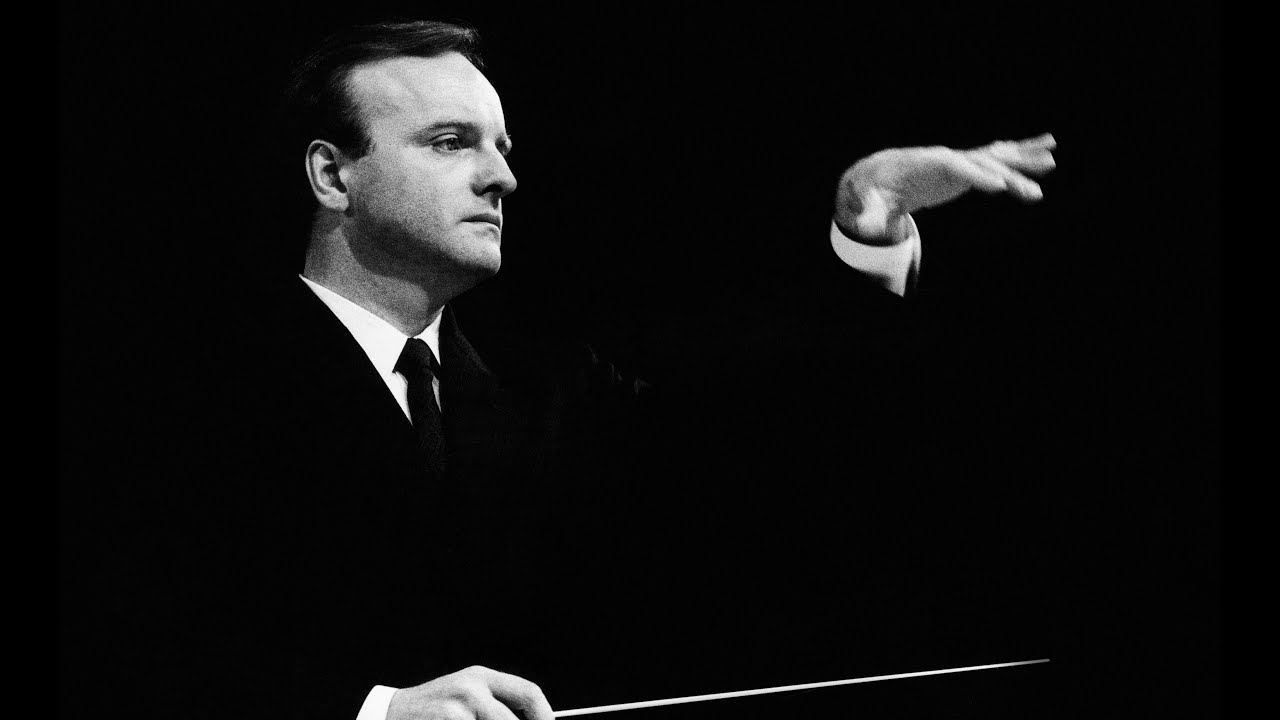
\includegraphics[width=0.48\linewidth]{pictures/youtube/2025/06/20250603_220510_youtube_002_v0lMWnBzUkY.jpg}
}
\end{center}




アーノンクール、マタイ受難曲　← 古楽

\url{https://youtu.be/5ZtyHJWBR1s}

\begin{center}
\href{https://youtu.be/5ZtyHJWBR1s}{

\includegraphics[width=0.48\linewidth]{pictures/youtube/2025/06/20250603_220510_youtube_003_5ZtyHJWBR1s.jpg}
}
\end{center}




イヴァン フィッシャー、マタイ受難曲　← お気に入り

\url{https://youtu.be/Tq4lxMcwYwU}

\begin{center}
\href{https://youtu.be/Tq4lxMcwYwU}{
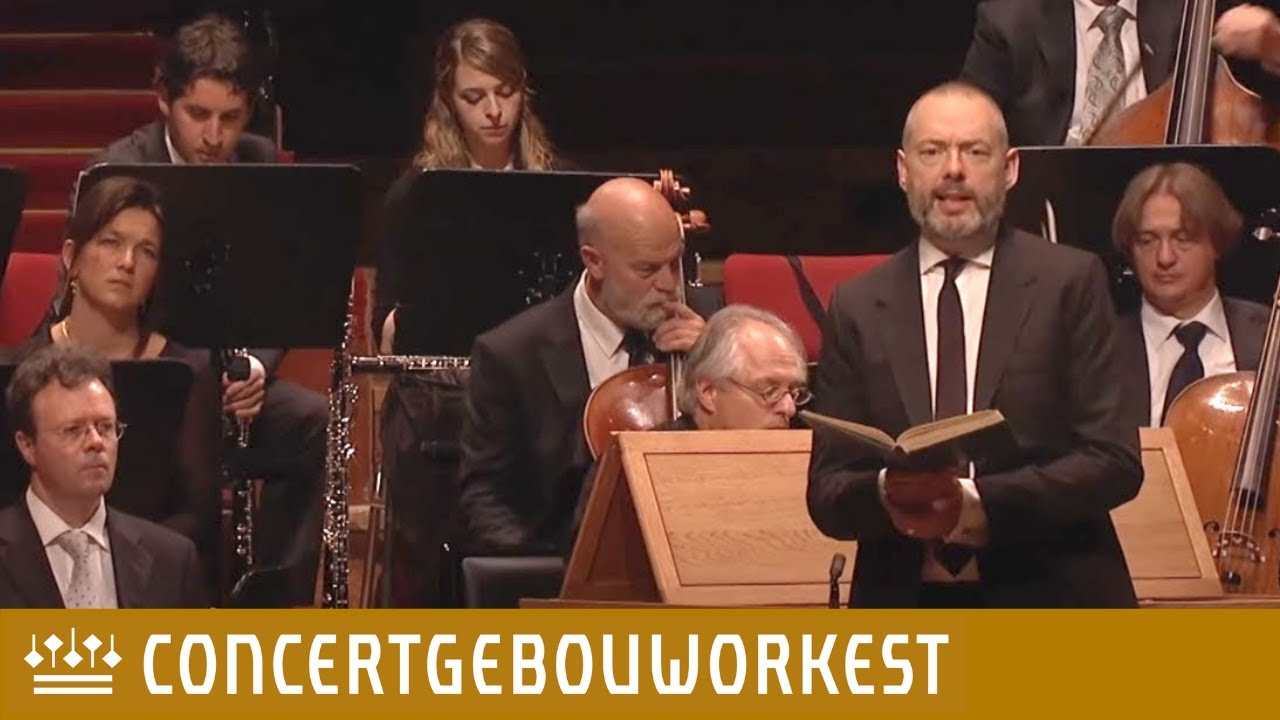
\includegraphics[width=0.48\linewidth]{pictures/youtube/2025/06/20250603_220510_youtube_004_Tq4lxMcwYwU.jpg}
}
\end{center}



\subsection*{2025年06月04日 00:08}
\addcontentsline{toc}{subsection}{2025年06月04日 00:08}

モーツァルトの絶筆、ラクリモサ

\url{https://youtu.be/AX9hrrcPjWc}

\begin{center}
\href{https://youtu.be/AX9hrrcPjWc}{
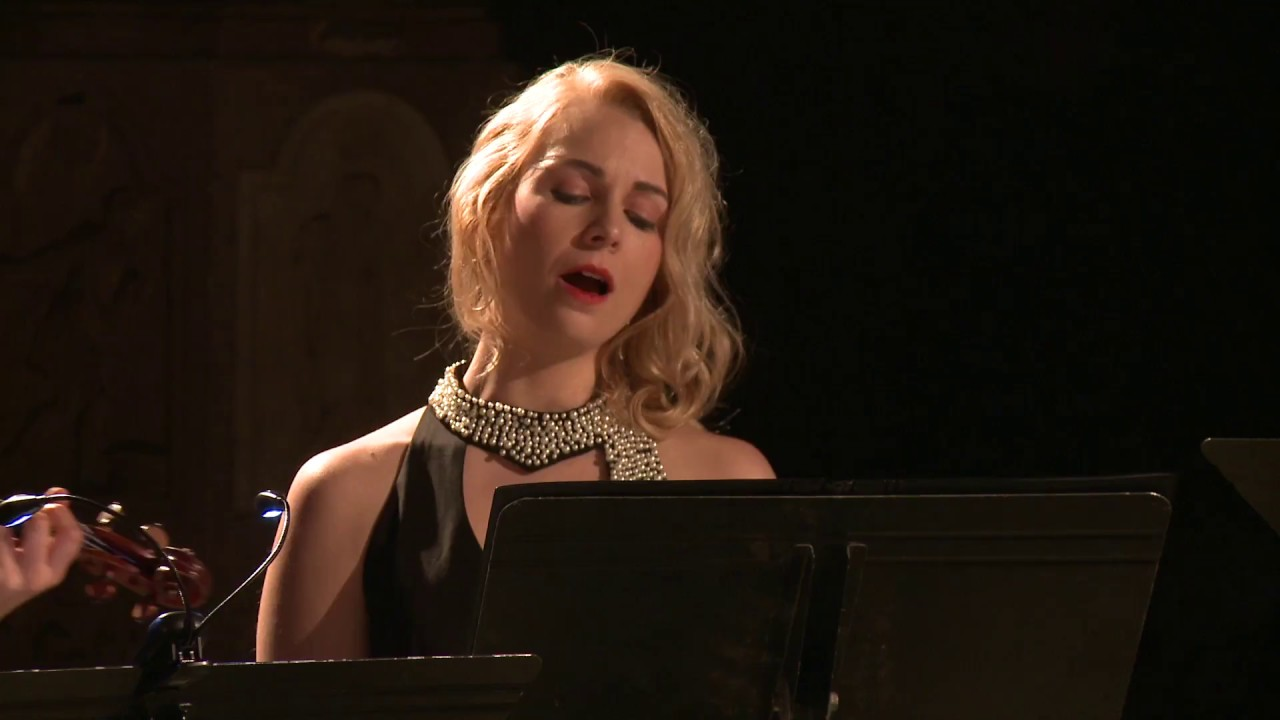
\includegraphics[width=0.48\linewidth]{pictures/youtube/2025/06/20250604_000836_youtube_001_AX9hrrcPjWc.jpg}
}
\end{center}




カールベーム、ウィーンフィル、モツレク

\url{https://youtu.be/-1DsJ5YQr5s}

\begin{center}
\href{https://youtu.be/-1DsJ5YQr5s}{
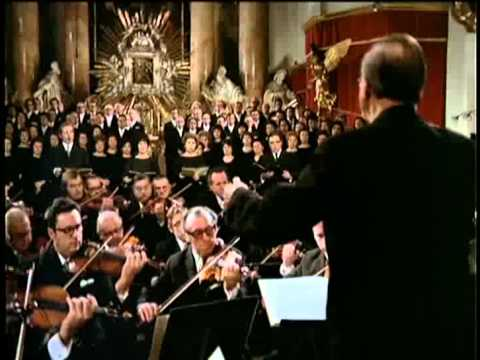
\includegraphics[width=0.48\linewidth]{pictures/youtube/2025/06/20250604_000836_youtube_002_-1DsJ5YQr5s.jpg}
}
\end{center}



唯一無二最高のモツレク。ゆっくりのテンポが良い。29分15秒辺りからラクリモサに入るが、合唱もオケもベームのゆっくりめのテンポへの対応が大変そうだ。ラストの「アーメン」がと〜っても長い。ベームとウイーン・フィルのこの曲の演奏（録音）がこの様な形で残されている事に感謝だ。（カール・ベームも若い）


アヴェヴェルムコルプス（心が洗われる様です）

\url{https://youtu.be/gDKCK_6WLTg}

\begin{center}
\href{https://youtu.be/gDKCK_6WLTg}{
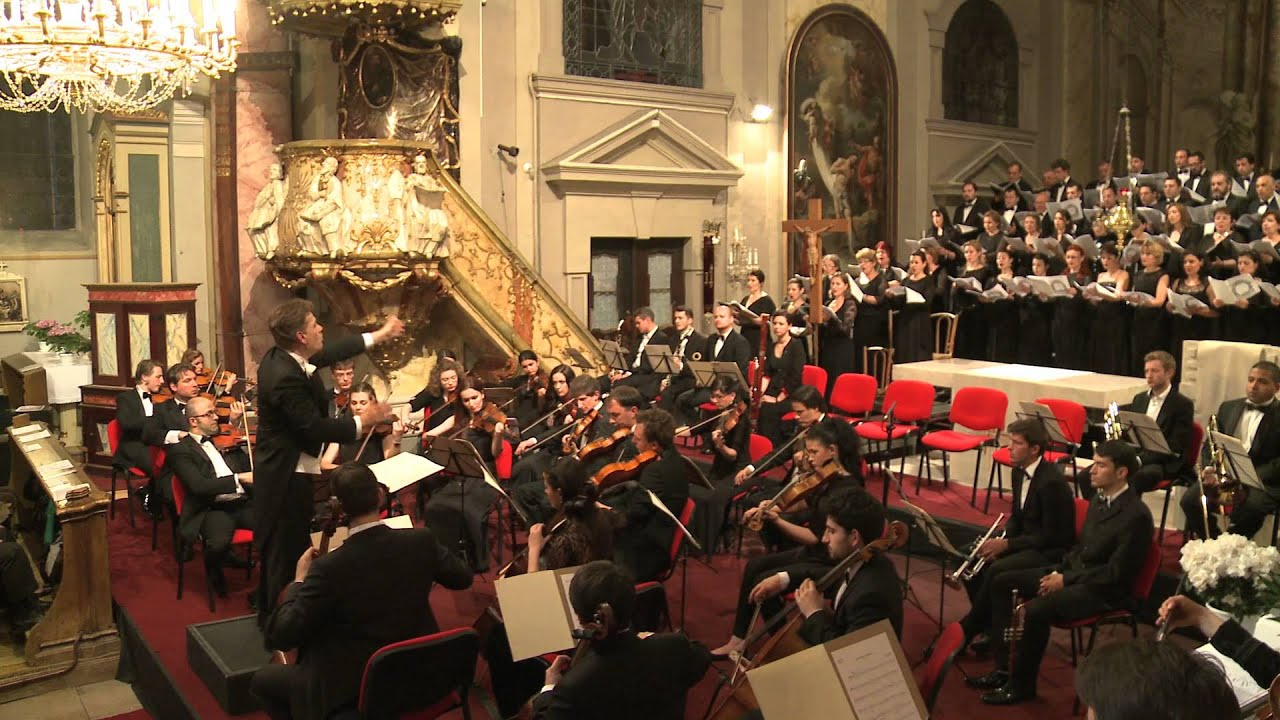
\includegraphics[width=0.48\linewidth]{pictures/youtube/2025/06/20250604_000836_youtube_003_gDKCK_6WLTg.jpg}
}
\end{center}



\subsection*{2025年06月04日 00:19}
\addcontentsline{toc}{subsection}{2025年06月04日 00:19}

\paragraph{リンク}
\url{https://youtu.be/of-WOH-uxYs}

\begin{center}
\href{https://youtu.be/of-WOH-uxYs}{
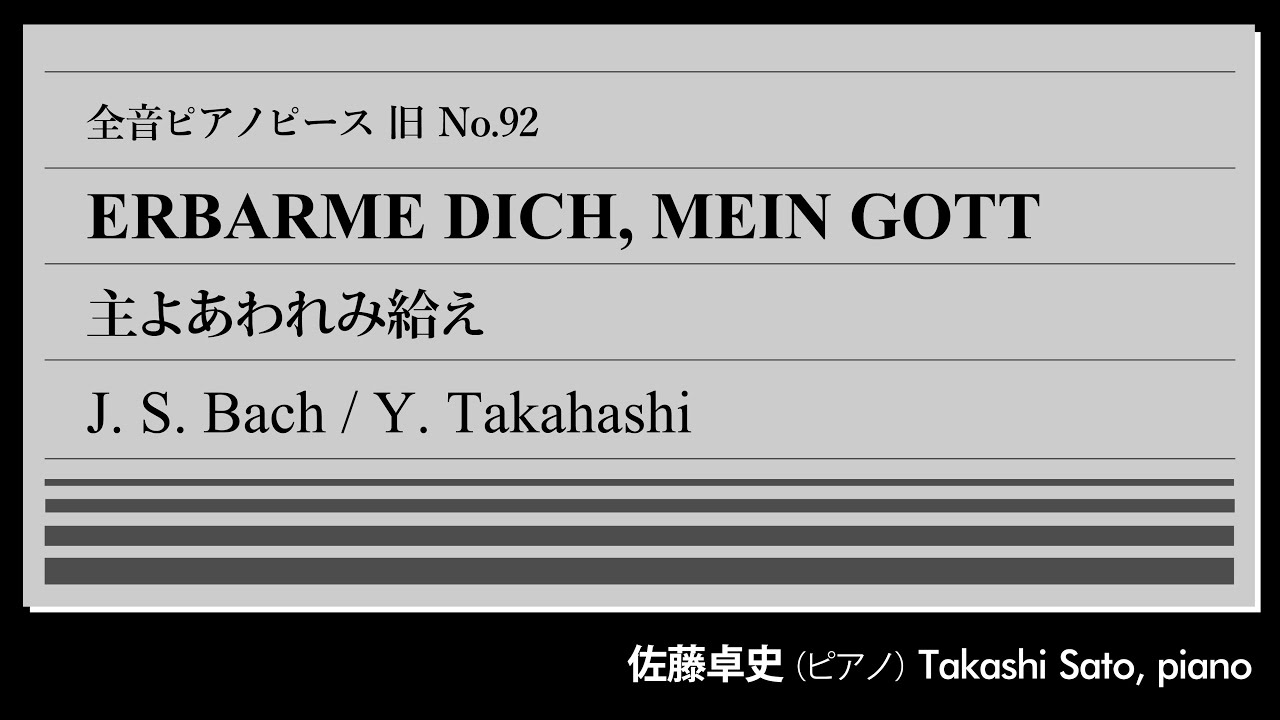
\includegraphics[width=0.48\linewidth]{pictures/youtube/2025/06/20250604_001910_youtube_001_of-WOH-uxYs.jpg}
}
\end{center}

\subsection*{2025年06月04日 20:13}
\addcontentsline{toc}{subsection}{2025年06月04日 20:13}

\paragraph{リンク}
\url{https://www.kanazawa-kentei.com/index.php}

\subsection*{2025年06月04日 21:58}
\addcontentsline{toc}{subsection}{2025年06月04日 21:58}

\paragraph{リンク}
\url{https://www.kanazawa21.jp/data_list.php?g=25&d=2182}

\subsection*{2025年06月05日 00:03}
\addcontentsline{toc}{subsection}{2025年06月05日 00:03}

\paragraph{リンク}
\url{https://www.businesstoday.in/technology/news/story/700-indian-engineers-posed-as-ai-the-london-startup-that-took-microsoft-for-a-ride-478514-2025-05-31}

\subsection*{2025年06月07日 11:03}
\addcontentsline{toc}{subsection}{2025年06月07日 11:03}

\url{https://www.aozora.gr.jp/cards/000042/files/2449_11267.html}



これは面白い🤣

おそらく「 \#待ち行列 」の問題としてシミュレーションできるものかもしれません。

\#キュー がシリーズになっていて、各キューには呼が \#ランダム到着 して、各キューでのサービスは、ランダムではなくてある程度スケジュールされているわけですが、ばらつきはある。どんな時間間隔、サービス時間はどうしたらいい？

\#寺田寅彦 氏が色々考察して下さっていますし、それを参照しながら、真面目に取り組んでみたら面白そうです。

\subsection*{2025年06月08日 01:32}
\addcontentsline{toc}{subsection}{2025年06月08日 01:32}

\#Cello組曲 は、さてさて何処から手をつけたらいいものでしょうか？

最後の曲6番（\#BWV1012 ）も魅力的ではありますが、やっぱりオーソドックスに、先ずは一番最初の曲（ \#BWV1007 の \#Prelude ）は押さえておきたいものです。

これから楽譜を探してみようかな（演奏に挑戦するかどうかは別にして）。3弦がFis でない（Gのままの）楽譜の中から探します。第3弦を半音下げるのは、ちょっとその世界に飛び込む勇気はありません。6弦Dまでは許せるけど、加えて3弦Fis って言われると、楽譜見ていて頭の中が混乱してしまう様な気がするから。運指を初めから自分で考え直せばいいんだろうけど、やっぱり識者の運指を知った上で、素人としての都合に合わせた運指にする事なら、なんとかなるかもしれないとは思います。


Prelude（Irina Kulikova編）

\url{https://youtu.be/xiEZPRg3p_g}

\begin{center}
\href{https://youtu.be/xiEZPRg3p_g}{
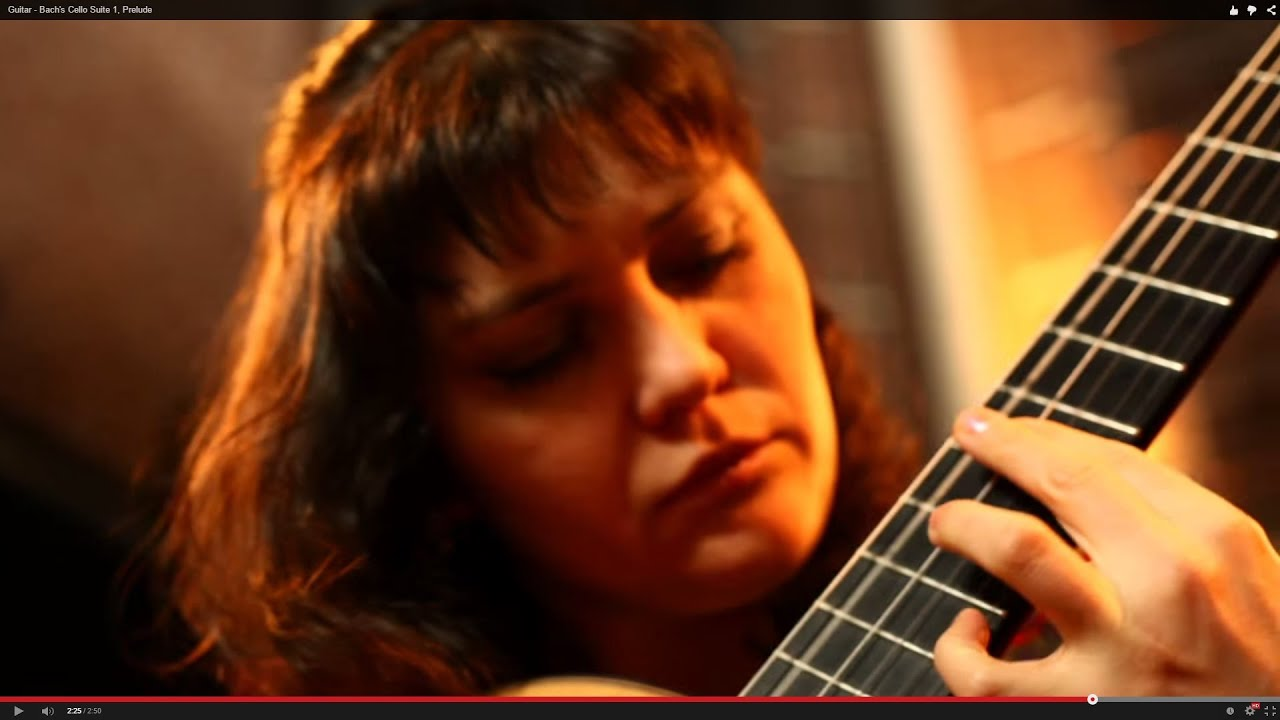
\includegraphics[width=0.48\linewidth]{pictures/youtube/2025/06/20250608_013250_youtube_001_xiEZPRg3p_g.jpg}
}
\end{center}




この方の演奏も良い（Michael Langer編）

\url{https://youtu.be/C5IHqqUZEYk}

\begin{center}
\href{https://youtu.be/C5IHqqUZEYk}{
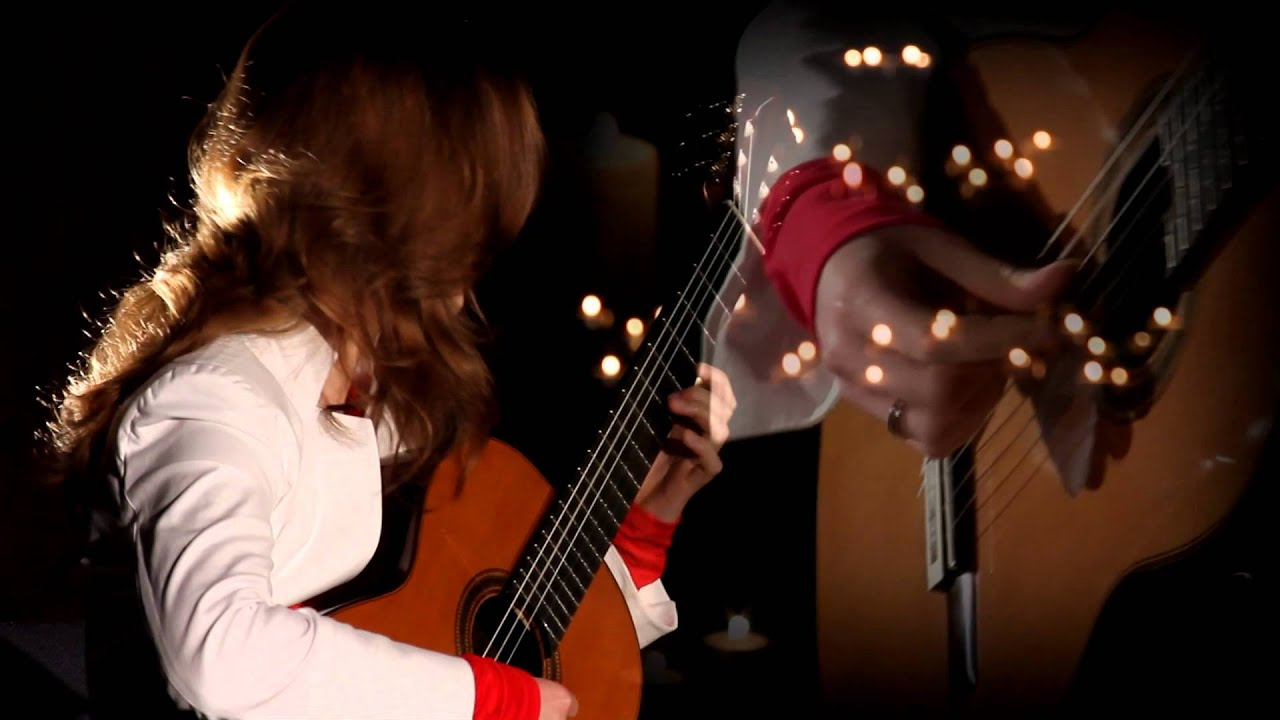
\includegraphics[width=0.48\linewidth]{pictures/youtube/2025/06/20250608_013250_youtube_002_C5IHqqUZEYk.jpg}
}
\end{center}



ゆっくり：

\url{https://youtu.be/3FBn12W9pS4}

\begin{center}
\href{https://youtu.be/3FBn12W9pS4}{
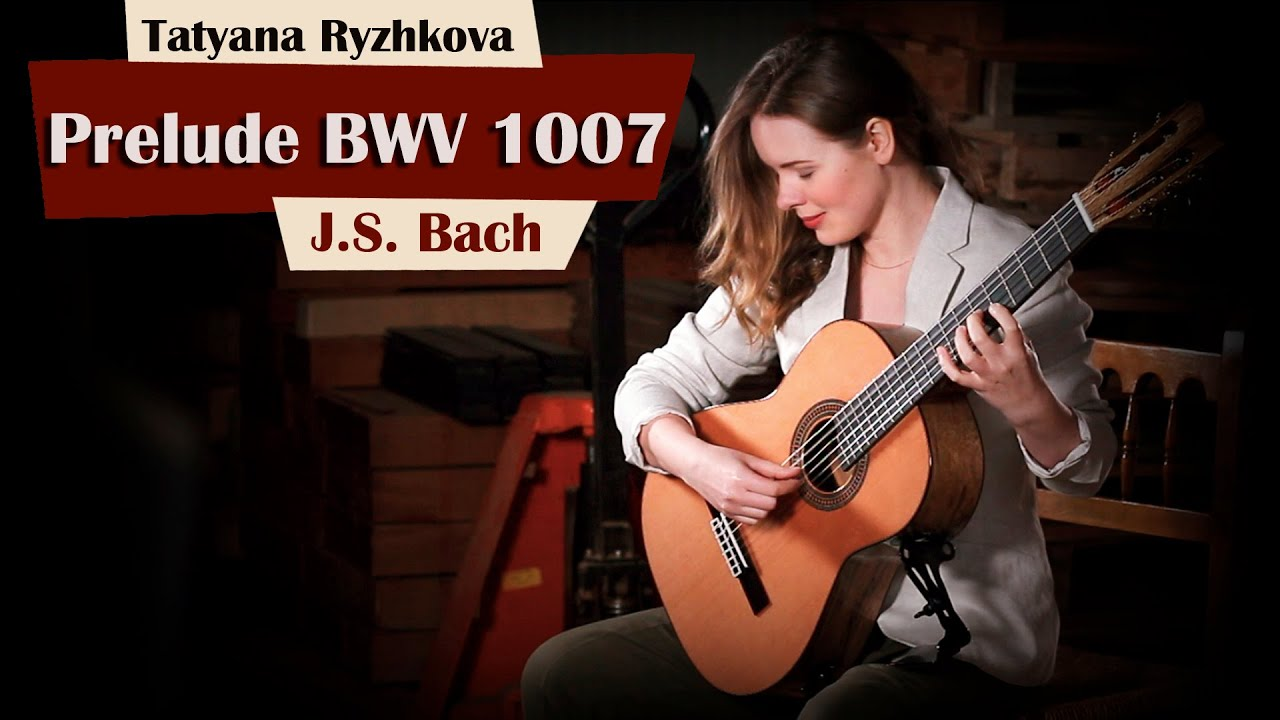
\includegraphics[width=0.48\linewidth]{pictures/youtube/2025/06/20250608_013250_youtube_003_3FBn12W9pS4.jpg}
}
\end{center}



\subsection*{2025年06月08日 14:55}
\addcontentsline{toc}{subsection}{2025年06月08日 14:55}

\paragraph{リンク}
\url{https://youtu.be/HNrq-j3wzM4}

\begin{center}
\href{https://youtu.be/HNrq-j3wzM4}{
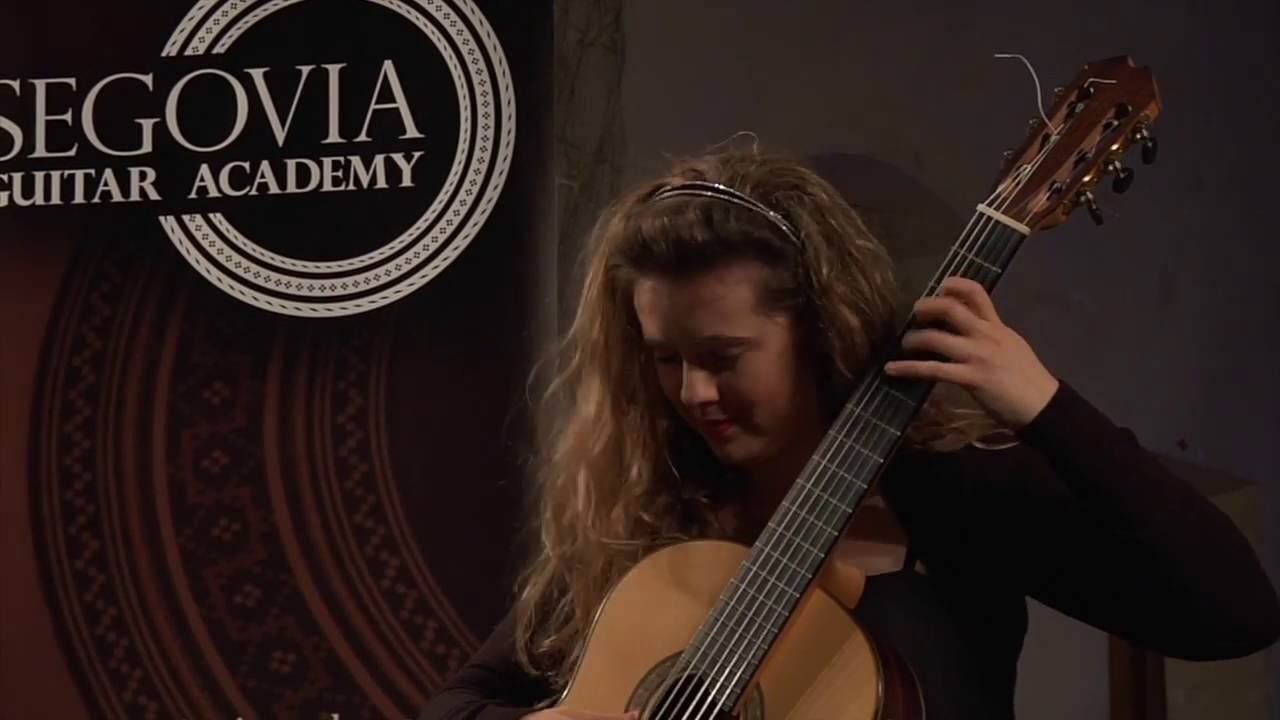
\includegraphics[width=0.48\linewidth]{pictures/youtube/2025/06/20250608_145518_youtube_001_HNrq-j3wzM4.jpg}
}
\end{center}

\subsection*{2025年06月09日 00:02}
\addcontentsline{toc}{subsection}{2025年06月09日 00:02}

\paragraph{リンク}
\url{https://youtu.be/uo19A_HVhFI}

\begin{center}
\href{https://youtu.be/uo19A_HVhFI}{
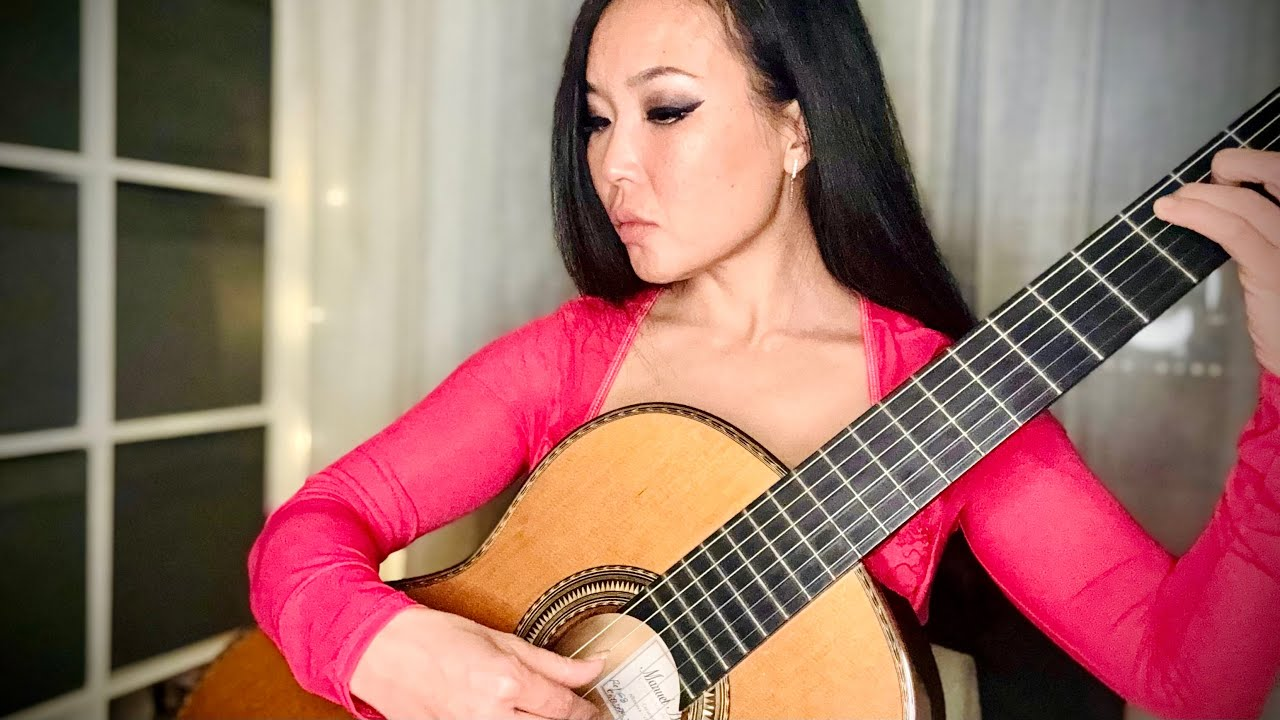
\includegraphics[width=0.48\linewidth]{pictures/youtube/2025/06/20250609_000219_youtube_001_uo19A_HVhFI.jpg}
}
\end{center}

\subsection*{2025年06月09日 08:14}
\addcontentsline{toc}{subsection}{2025年06月09日 08:14}

\paragraph{リンク}
\url{https://youtu.be/R7WMnJoauL8}

\begin{center}
\href{https://youtu.be/R7WMnJoauL8}{
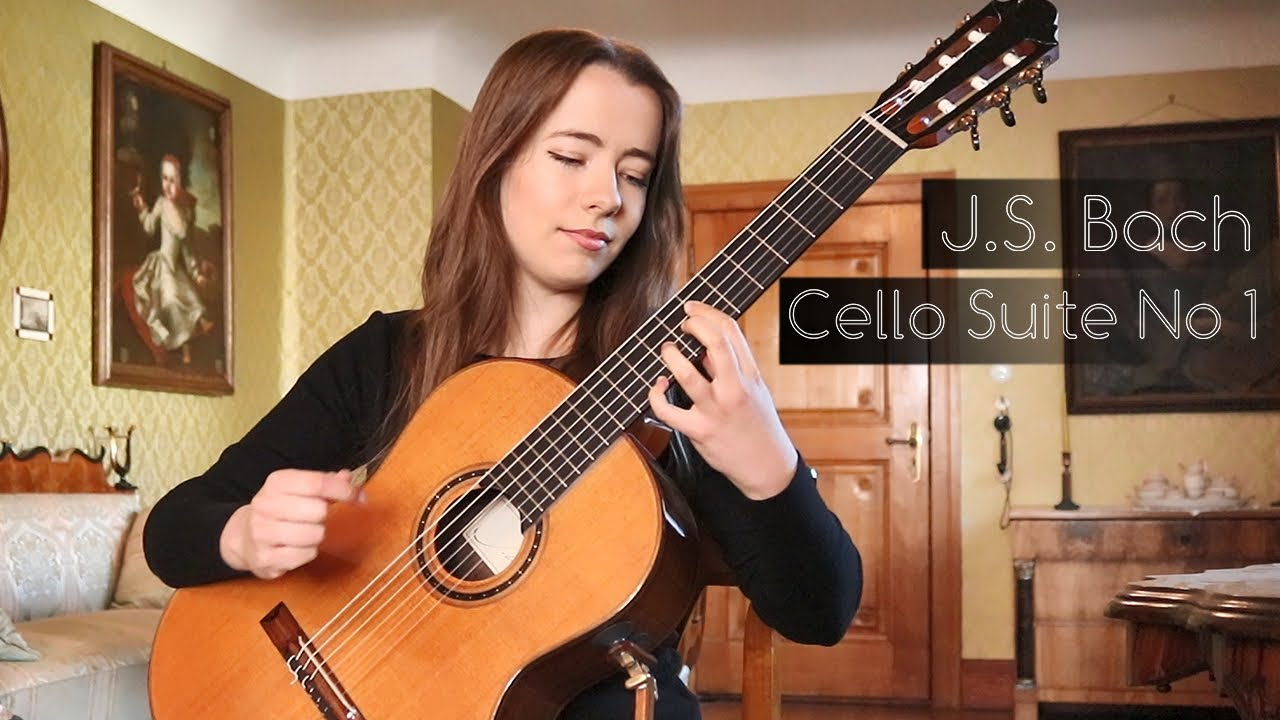
\includegraphics[width=0.48\linewidth]{pictures/youtube/2025/06/20250609_081408_youtube_001_R7WMnJoauL8.jpg}
}
\end{center}

\subsection*{2025年06月09日 08:16}
\addcontentsline{toc}{subsection}{2025年06月09日 08:16}

\paragraph{リンク}
\url{https://youtu.be/xiEZPRg3p_g}

\begin{center}
\href{https://youtu.be/xiEZPRg3p_g}{
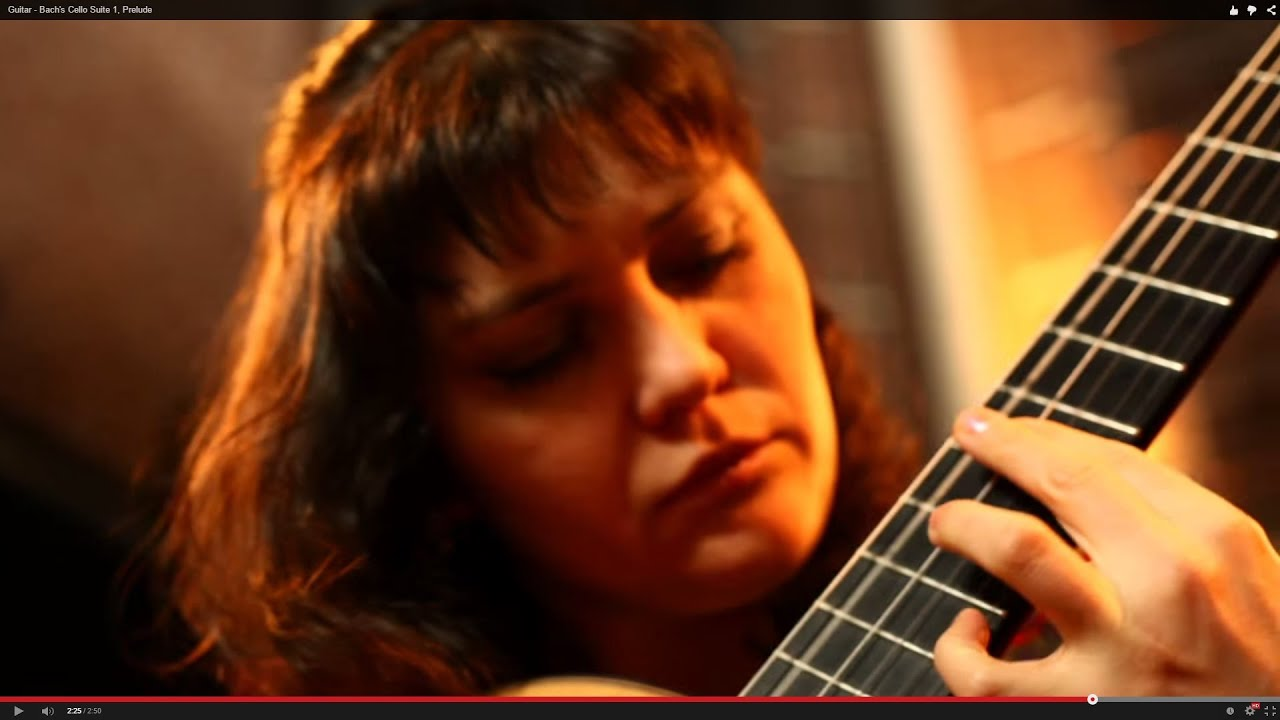
\includegraphics[width=0.48\linewidth]{pictures/youtube/2025/06/20250609_081643_youtube_001_xiEZPRg3p_g.jpg}
}
\end{center}

\subsection*{2025年06月12日 01:04}
\addcontentsline{toc}{subsection}{2025年06月12日 01:04}

What a wonderful world.


鈴木大介編

\url{https://youtu.be/hrsFr48-MYg}

\begin{center}
\href{https://youtu.be/hrsFr48-MYg}{
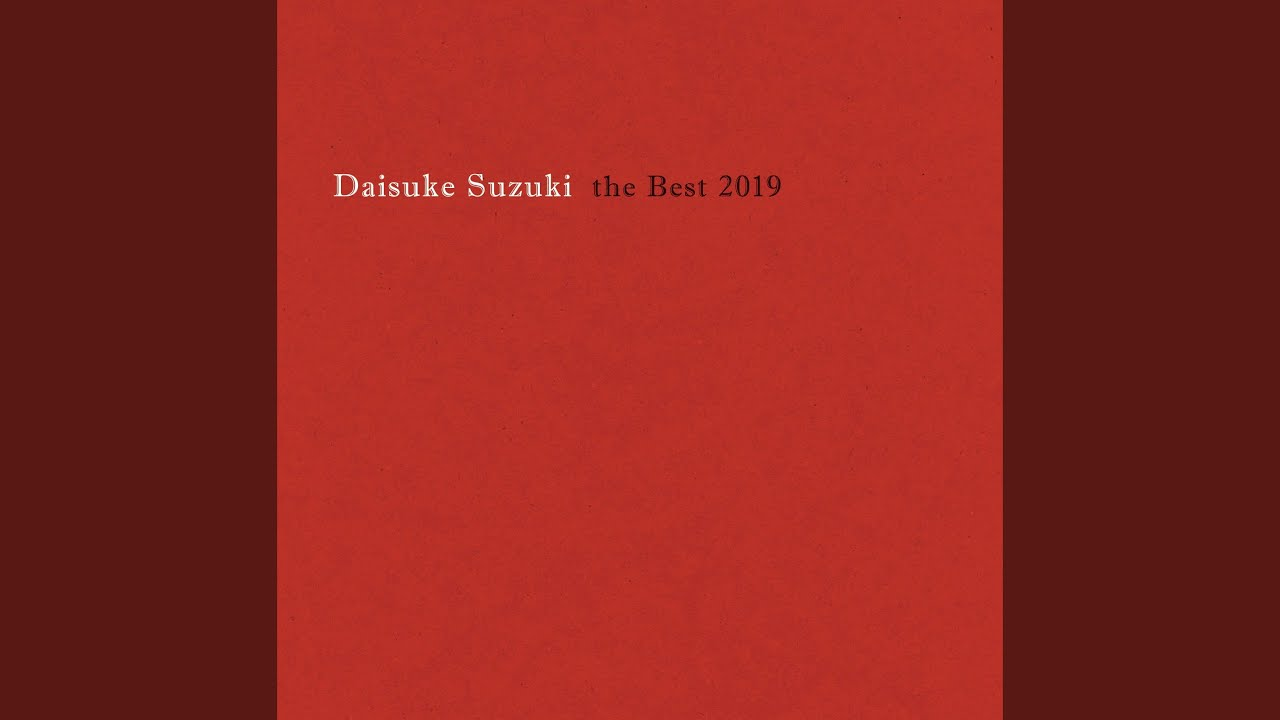
\includegraphics[width=0.48\linewidth]{pictures/youtube/2025/06/20250612_010411_youtube_001_hrsFr48-MYg.jpg}
}
\end{center}




楽譜はここ

\url{https://www.gendaiguitar.com/products/4539442063404}




歌詞

I see trees of green, red roses too

I see them blue before me and you

And I think to myself

What a wonderful world


I see skies of blue and clouds of white

The bright blessed day, the dark sacred night

And I think to myself

What a wonderful world


The colors of the rainbow so pretty in the sky

Or also on the faces of people going by

I see friends shaking hands, saying "How do you do?"

They're really saying, I love you


I hear babies crying, I watch them them grow

They'll learn much more and I'll never know

And I think to myself

What a wonderful world

Yes, I think to myself

What a wonderful world


Oh yeah

\subsection*{2025年06月12日 08:29}
\addcontentsline{toc}{subsection}{2025年06月12日 08:29}

懐かしい。\#AppleⅡ の勇姿ですね。


学生の頃ですが、NECのTK-80（組み立てキットのボードコンピュータでCPUは8080）の一台を皆んなで取り囲んで覗き込んでいた、そんな時代でした。ある日AppleⅡが一台導入されて、科の印刷室に置かれました。印刷室なので学生用に導入されたものではなかったみたいでしたが、当時卒論で有限要素（FEM）解析をしていた私は、毎日占有する様にして使わせてもらいました。


卒論では、机上でデータを準備しては計算機センターへ行ってそれをカードに打ち込み、そこでFEMのプログラムをsubmitして、プリンタからの出力結果を受け取るということをしていました。プログラムに渡すデータですが、隣り合う数値の差をある一定の値以下にしなければなりませんでした。（専門用語を厭わないなら、スパースマトリクスのバンド幅に納める必要があった、という事）そこで、机上で用意したデータを、AppleⅡのBASICのDATA文として入力して、プログラムでバンド幅に収まっているかどうかをチェックしていたというのが、AppleBASICに出会ったきっかけでした。チェックに引っかかると、それを直してはあらためてチェックして、という事を繰り返して、チェックに通った結果を計算機センターへ持って行って、カードパンチして、サブミットして、、という事をしていました。


それが一段落すると、FEMのプログラムそのものをAppleBASICで動かせないかと思う様になり、計算機センターで動かしていたFEMのプログラム（FORTRANで書かれていた）をAppleBASICに移そうとして、AppleⅡの前に四六時中座り込んで奮闘する日々を送る様になりました。印刷室だったので、当時、科の先生方が部屋に来られた際には「M （←私）の為に購入したみたいなものだな」と仰っていました。AppleⅡのCPUは6502というCPUでしたか？とにかく8ビットのCPUでメモリは最大でも64KByte（BASICインタープリタを含めたOSのROM領域を含む）でしたから、FEMのマトリクスのバンド幅にあるデータの全てを殆ど30KByte以下の中に収めて、その中で計算する必要がありました（自ずと扱える接点の総数も明らかでした）。ビデオRAMの領域も主記憶中にとられていましたが、そこもデータの領域として使っていました。とにかく「Out of memory」というエラーメッセージをしょっちゅう目にしていました。どうやってメモリ領域を稼いだらいいかに最後まで腐心、工夫していました。が、これは結局時間切れ、「動きませんでした」


という事で、懐かしいAppleⅡの勇姿に出会えて嬉しく思い、「超いいね」を押した記事でした。こんな綺麗な状態のAppleⅡは、おいくらなんでしょう？計算機ではなくて、歴史的な飾り物としての価値なんでしょうが、きっと高いことだろうと思います。

\paragraph{写真}
\begin{center}
\begin{minipage}{0.48\linewidth}
\centering
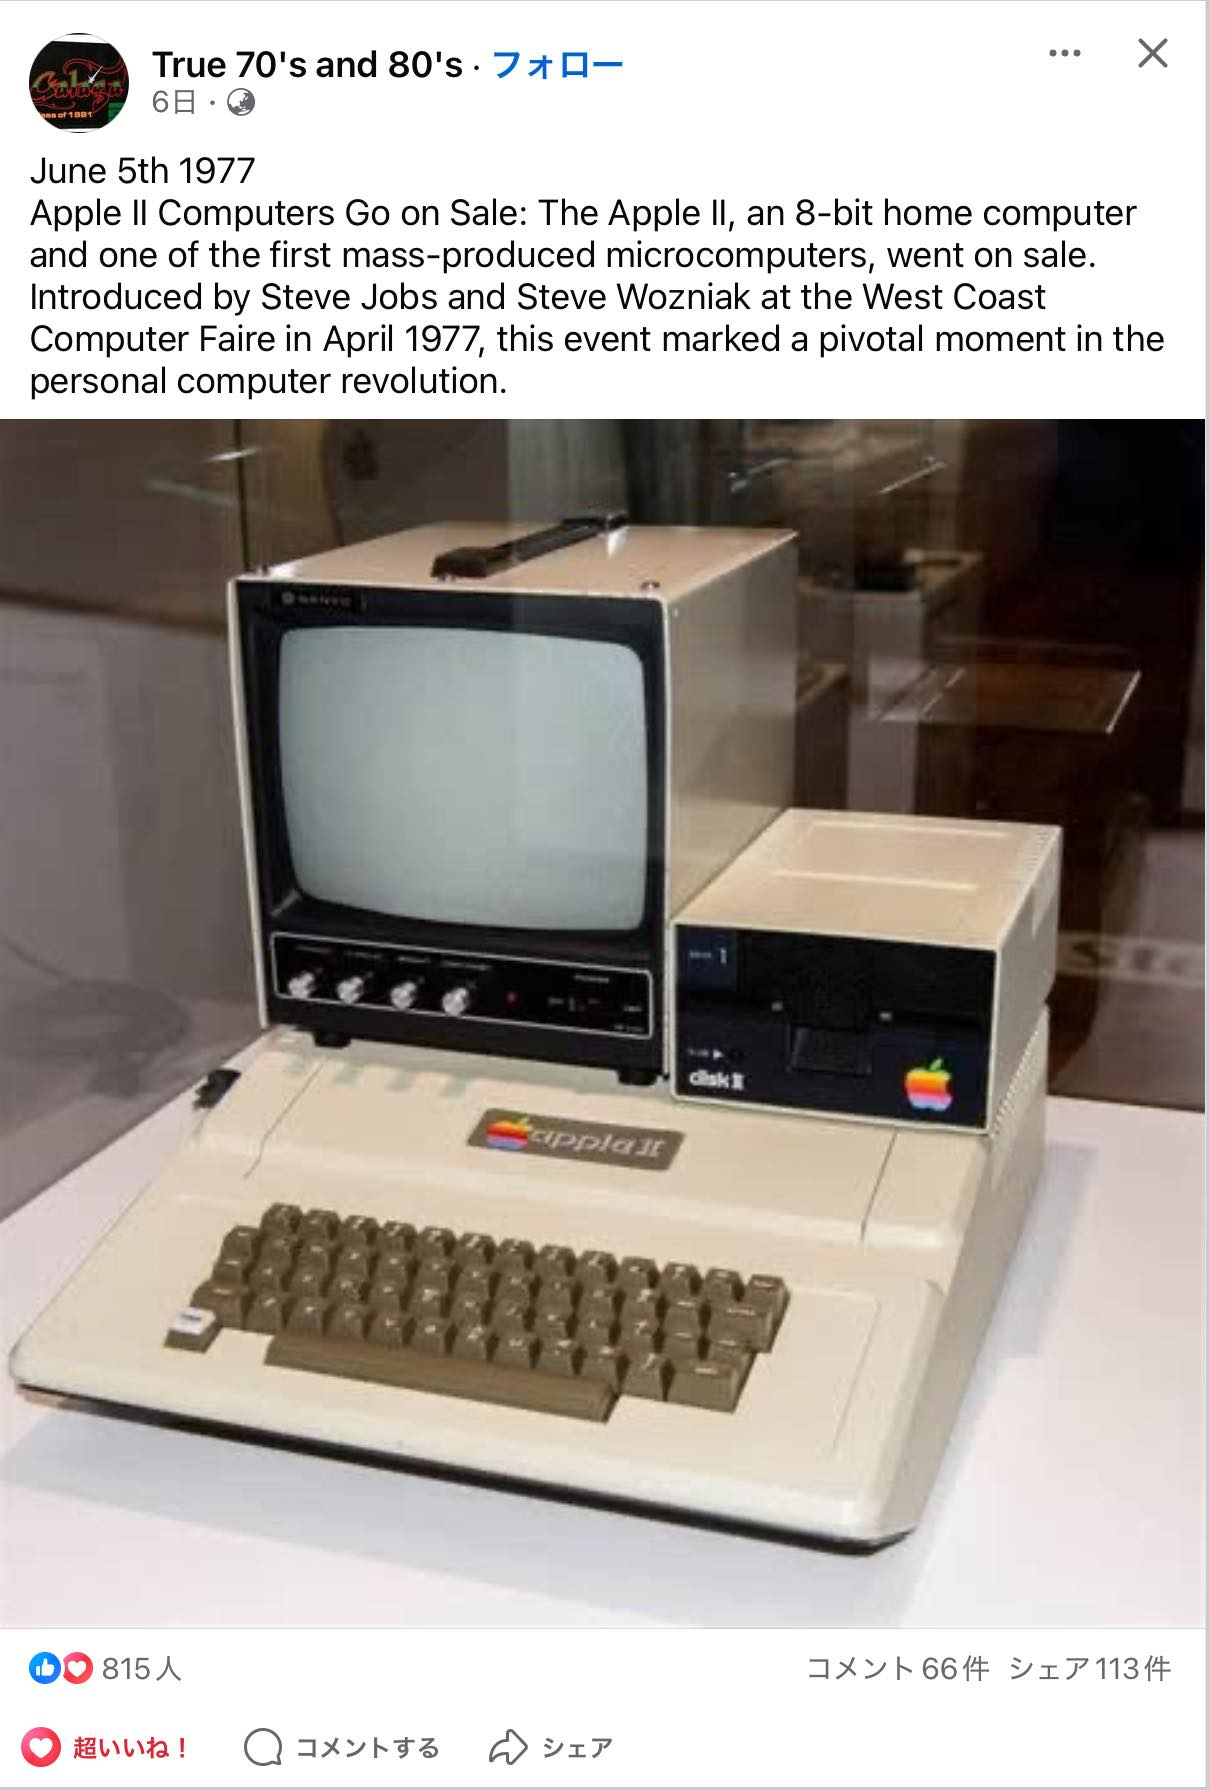
\includegraphics[width=\linewidth]{pictures/2025/06/20250612_082948_001.jpg}
\end{minipage}
\hfill
\begin{minipage}{0.48\linewidth}
\centering
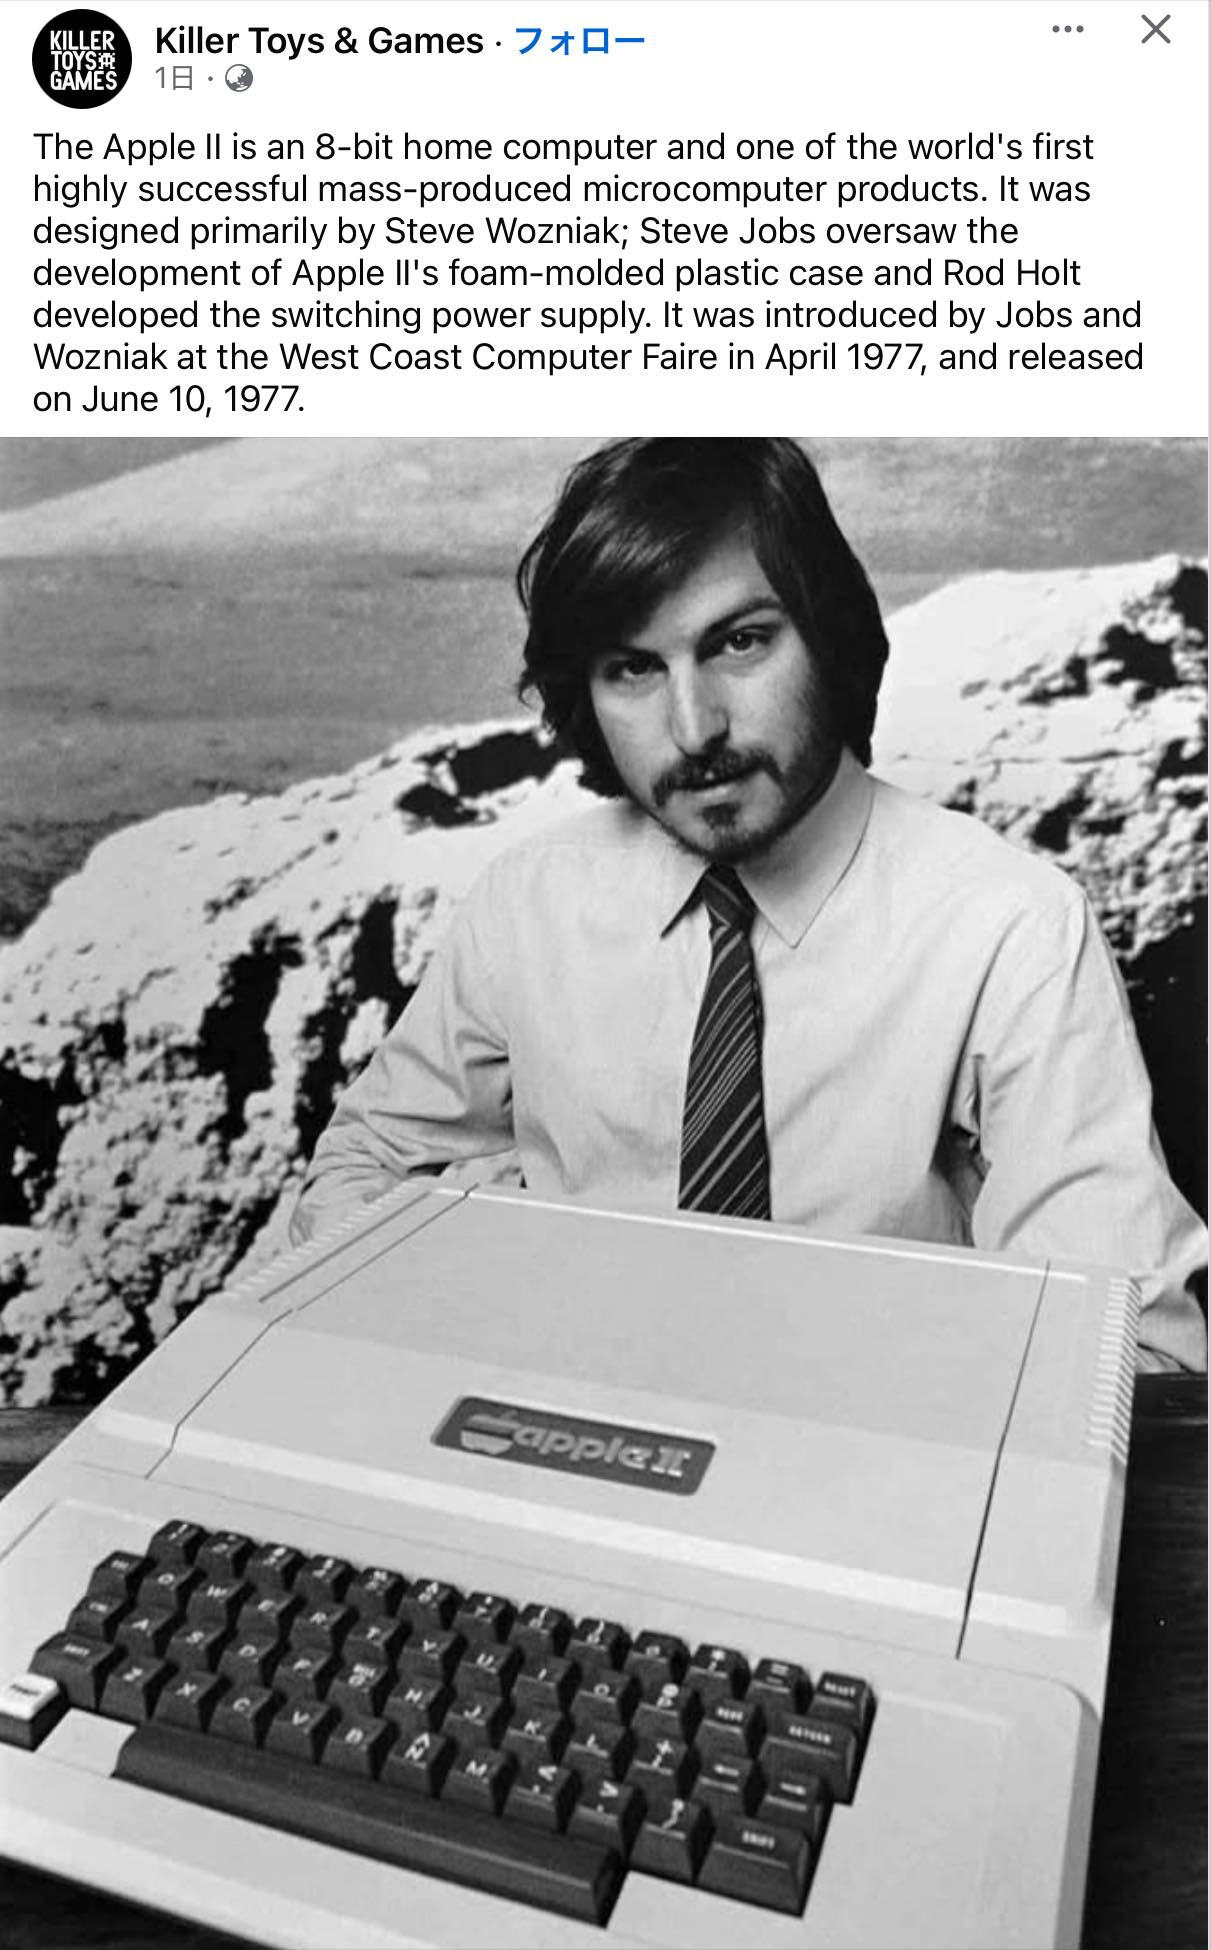
\includegraphics[width=\linewidth]{pictures/2025/06/20250612_082948_002.jpg}
\end{minipage}
\end{center}

\subsection*{2025年06月12日 17:25}
\addcontentsline{toc}{subsection}{2025年06月12日 17:25}

\paragraph{リンク}
\url{https://www.jstage.jst.go.jp/article/jjspm1947/30/8/30_8_306/_pdf}

\subsection*{2025年06月13日 11:19}
\addcontentsline{toc}{subsection}{2025年06月13日 11:19}

\paragraph{リンク}
\url{https://youtu.be/oQbnh8GdCwY}

\begin{center}
\href{https://youtu.be/oQbnh8GdCwY}{
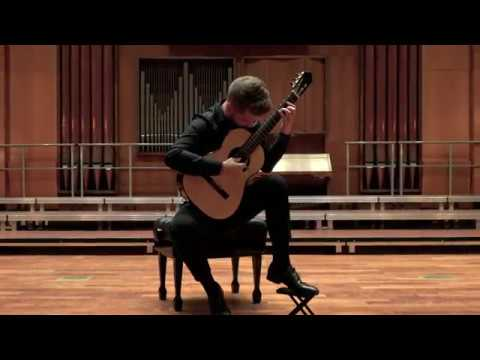
\includegraphics[width=0.48\linewidth]{pictures/youtube/2025/06/20250613_111930_youtube_001_oQbnh8GdCwY.jpg}
}
\end{center}

\subsection*{2025年06月15日 03:44}
\addcontentsline{toc}{subsection}{2025年06月15日 03:44}

\url{https://youtu.be/ECioFSIeexA}

\begin{center}
\href{https://youtu.be/ECioFSIeexA}{
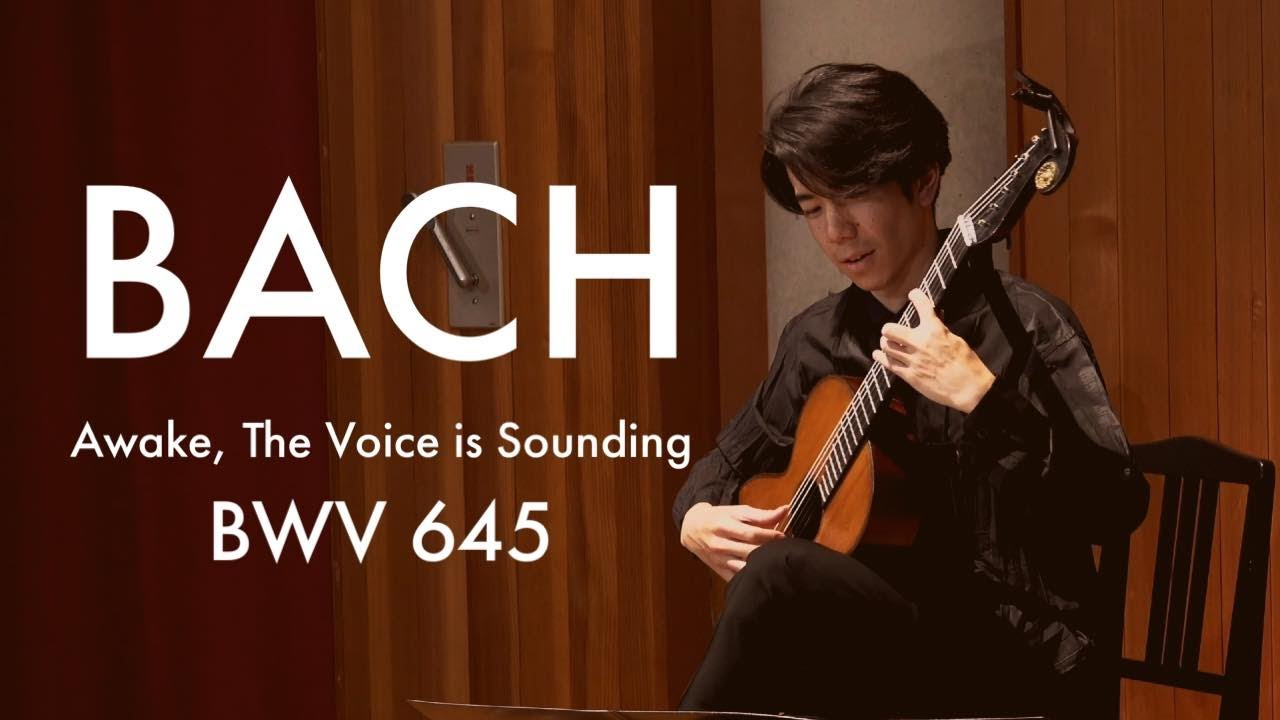
\includegraphics[width=0.48\linewidth]{pictures/youtube/2025/06/20250615_034443_youtube_001_ECioFSIeexA.jpg}
}
\end{center}




この方のギターも古いものかと思われますが、antiqueな音色をしています。どういう楽器なのかな。普通サイズ（650mm）じゃない様です（短いですね）。（ググってみると、この楽器は、ちょっと特異な形状を持つ19世紀のシュタウファーモデルというものらしい。長さは不明。）


装飾音はどう弾いてる？

\subsection*{2025年06月15日 05:46}
\addcontentsline{toc}{subsection}{2025年06月15日 05:46}

C.A.Debussyのベルガマスク組曲から月の光


（arrangement pour la guitare de James Bishop-Edwards ）

\url{https://youtu.be/0_RnlOWmZD4}

\begin{center}
\href{https://youtu.be/0_RnlOWmZD4}{
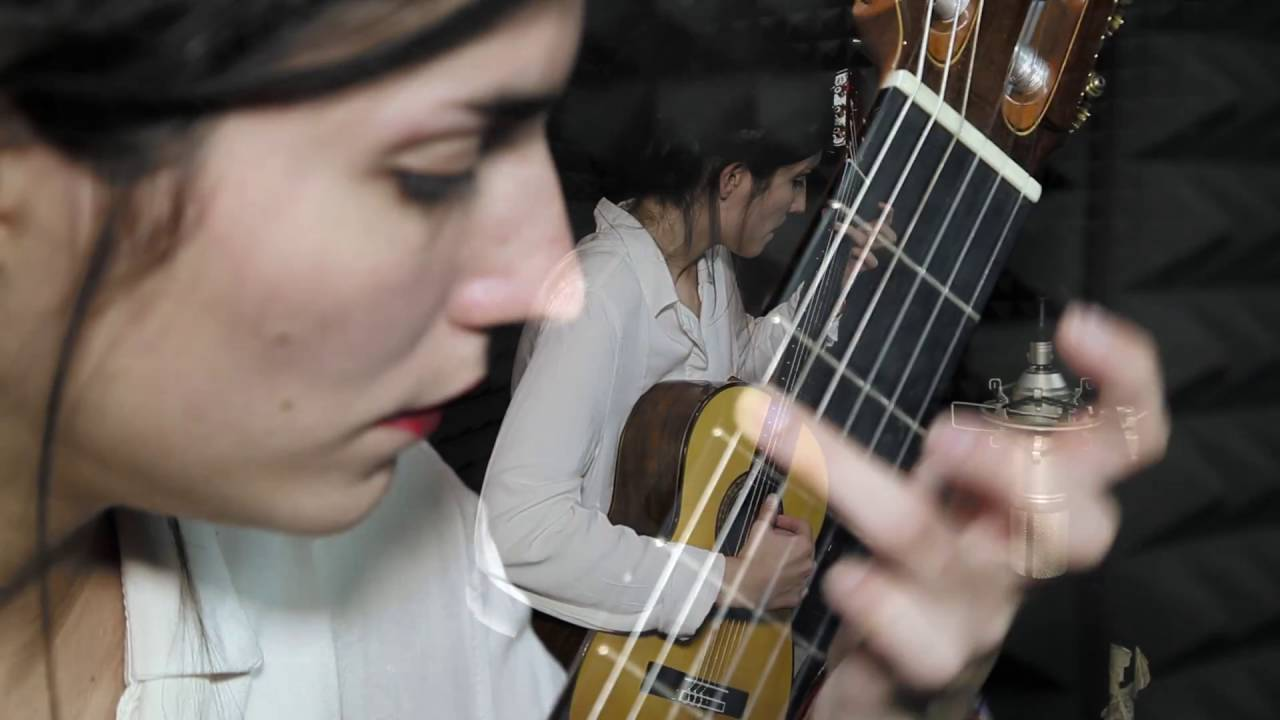
\includegraphics[width=0.48\linewidth]{pictures/youtube/2025/06/20250615_054622_youtube_001_0_RnlOWmZD4.jpg}
}
\end{center}




ギターの音域って広いんですねえ。編曲も演奏も素晴らしいな。

ギターの表現力や、その可能性について、大きさ、広さを痛感します。

ギターのために書かれた曲だったかと思ってしまうほどです。

\subsection*{2025年06月15日 09:08}
\addcontentsline{toc}{subsection}{2025年06月15日 09:08}

この投稿は公開しません（個人的な思い出です）


\url{https://www.jstage.jst.go.jp/article/jjspm1947/30/8/30_8_306/_pdf}




こんな所に自分の名前が載っているという事を、最近になって知りました。


上田完治先生は、最終的には東京大学の教授として引退されましたが、その昔（先生が若かった頃）は金沢大学工学部に助教授でいらした事があって、私はその時に卒論の指導をして頂きました。添付の論文は、私が卒業した後で発表された（学科名が変わっている）ものですが、内容は私にもよく分かります。


この論文中、アルミナ（Al2O3）セラミクスを想定した有限要素解析は私が卒論の時に計算していた時のものだと思います。ある日私は上田先生に部屋に呼ばれて、亀裂長さに対する歪みエネルギのグラフの線を引く時に行っていた、最小二乗近似による係数の導出を、この部屋でやり直してみるように言われました。先生は机に向かって何か仕事していらっしゃいましたが、その後ろの机で先生の後ろ姿を見ながら、電卓を使って（焦ってバタバタと）計算していたと思います。計算結果は、以前導いていた値と違った値になりました。「すいません、違っていました」と言ったら、もう一回落ち着いて計算し直してみるように言われました。静かな部屋の中で再計算していると、1回目よりも落ち着いて計算できた様に思います。計算結果は以前計算していた値と一致しました。よかった〜と思って、先生にその事を申し上げましたら、もう一回やってみてくれと言われ、最終的に4回程再計算したと思います。そう言えば「電卓の無い頃はもっと大変だったんだよ」という様な話もされていました。


また、当時この様な論文に載せる図は、ロットリングで描いたりして、切った貼ったしたものを、写真撮影して、それを暗室で現像、引き伸ばしてプリントして作成していました。上田先生に言われて、暗室で作業したことがあります。印刷できたものを見せると、もっと細い線にならないかと仰って、何度か暗室で試行錯誤しては先生に見せていた記憶があります。その時は自分の卒論に載せるための図のつもりでいたと思いますが、この添付論文に載る図でもあったのかもしれません。


以上がこの添付の論文に対する私のcontributionです。私の名前を載せて下さっていることを、最近まで知りませんでした。先生に実際にお会いして、お礼やらご無沙汰などのご挨拶ができたら嬉しかったのですが、先生はもう亡くなられている様です。あの頃は、助教授になられたばかりの新進気鋭の爽やかな先生でいらっしゃいました。合掌です。ご冥福をお祈りいたします。

\subsection*{2025年06月16日 05:33}
\addcontentsline{toc}{subsection}{2025年06月16日 05:33}

\paragraph{リンク}
\url{https://youtu.be/OQqEg7Yu-_E}

\begin{center}
\href{https://youtu.be/OQqEg7Yu-_E}{
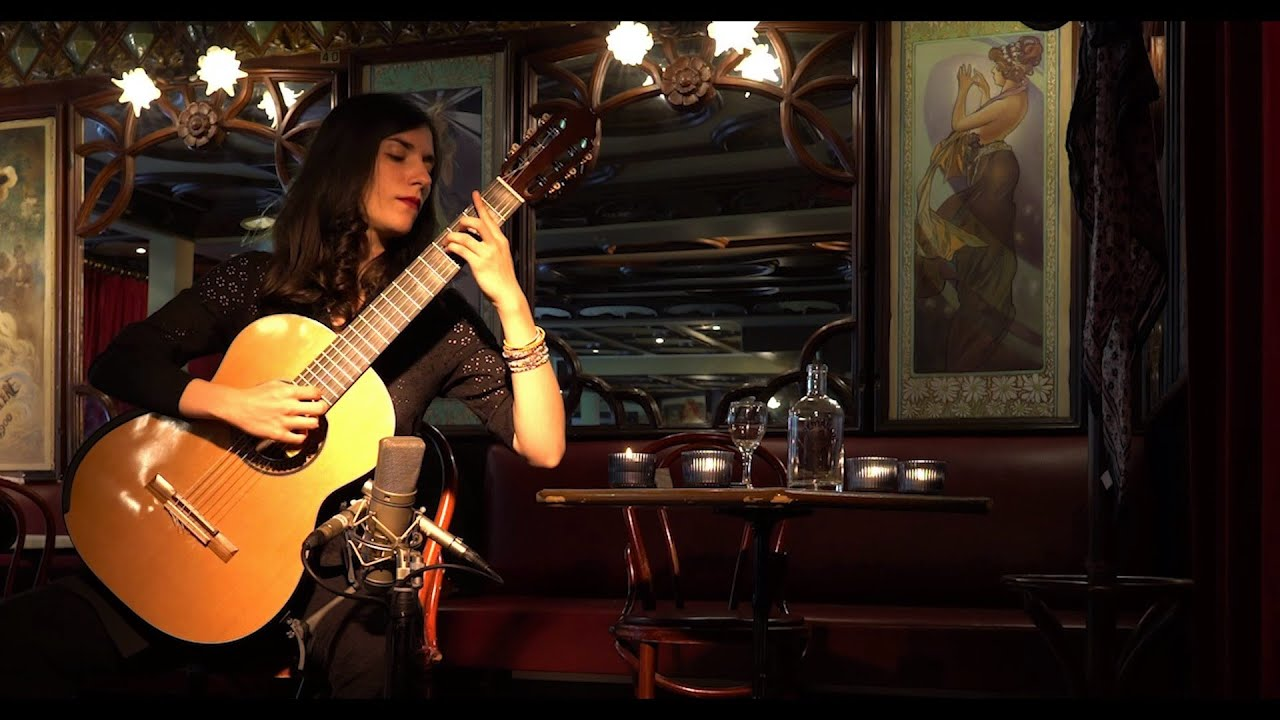
\includegraphics[width=0.48\linewidth]{pictures/youtube/2025/06/20250616_053326_youtube_001_OQqEg7Yu-_E.jpg}
}
\end{center}

\subsection*{2025年06月16日 05:45}
\addcontentsline{toc}{subsection}{2025年06月16日 05:45}

\paragraph{リンク}
\url{https://youtu.be/wF6pDOFtw3U}

\begin{center}
\href{https://youtu.be/wF6pDOFtw3U}{
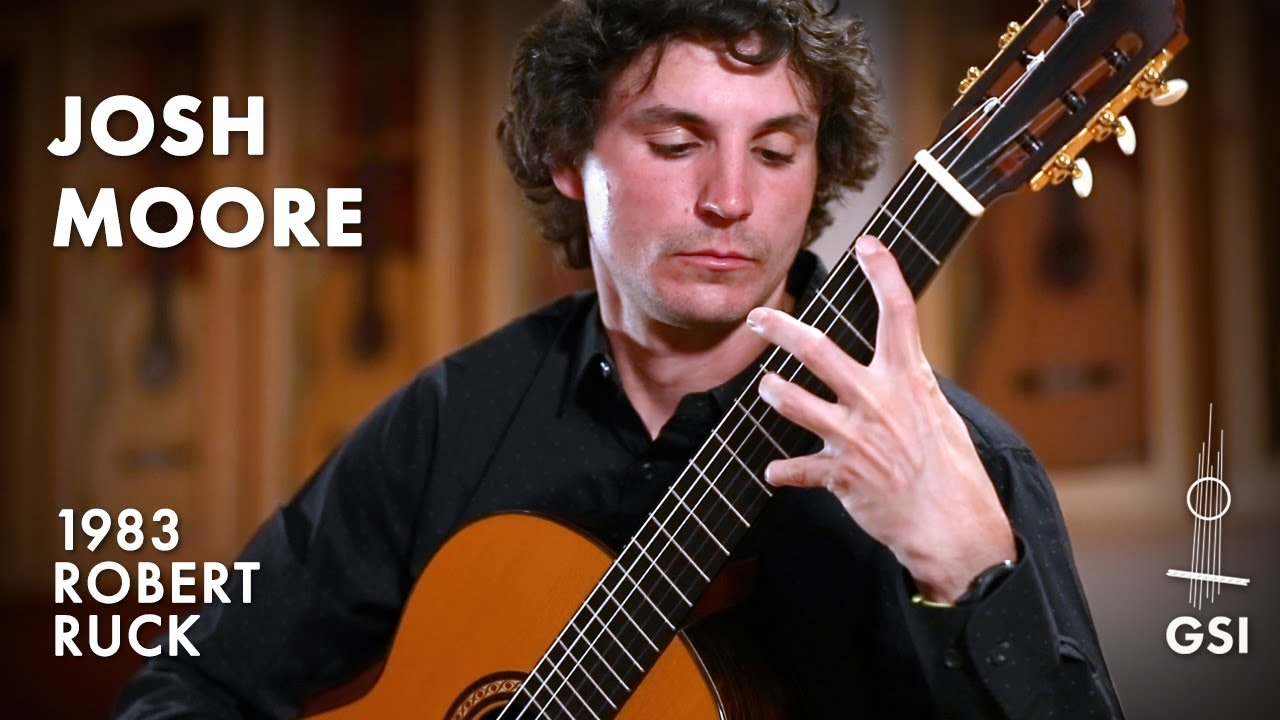
\includegraphics[width=0.48\linewidth]{pictures/youtube/2025/06/20250616_054519_youtube_001_wF6pDOFtw3U.jpg}
}
\end{center}

\subsection*{2025年06月16日 06:23}
\addcontentsline{toc}{subsection}{2025年06月16日 06:23}

\paragraph{リンク}
\url{http://taustation.com/conditional-probability-russian-roulette/}

\subsection*{2025年06月17日 01:49}
\addcontentsline{toc}{subsection}{2025年06月17日 01:49}

\paragraph{リンク}
\url{https://youtu.be/6kWbAXkhQjc}

\begin{center}
\href{https://youtu.be/6kWbAXkhQjc}{
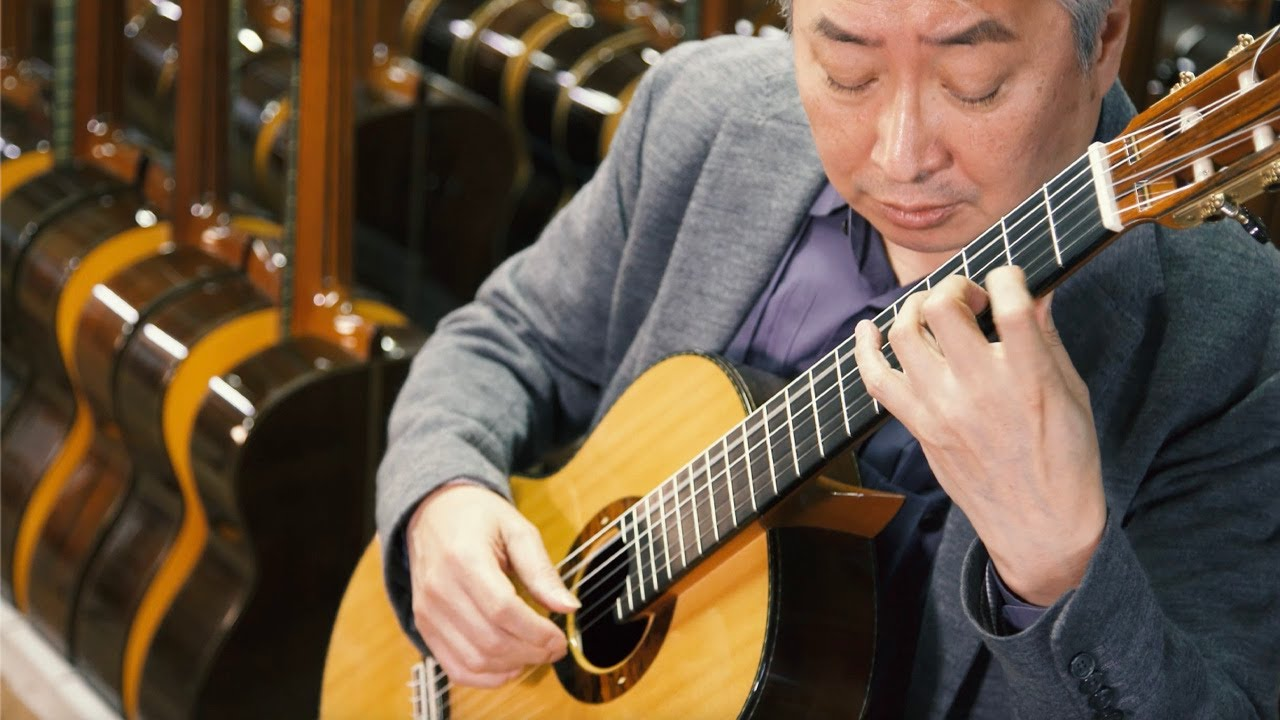
\includegraphics[width=0.48\linewidth]{pictures/youtube/2025/06/20250617_014918_youtube_001_6kWbAXkhQjc.jpg}
}
\end{center}

\subsection*{2025年06月17日 08:16}
\addcontentsline{toc}{subsection}{2025年06月17日 08:16}

\url{https://youtu.be/E19gz_uAM2Q}

\begin{center}
\href{https://youtu.be/E19gz_uAM2Q}{
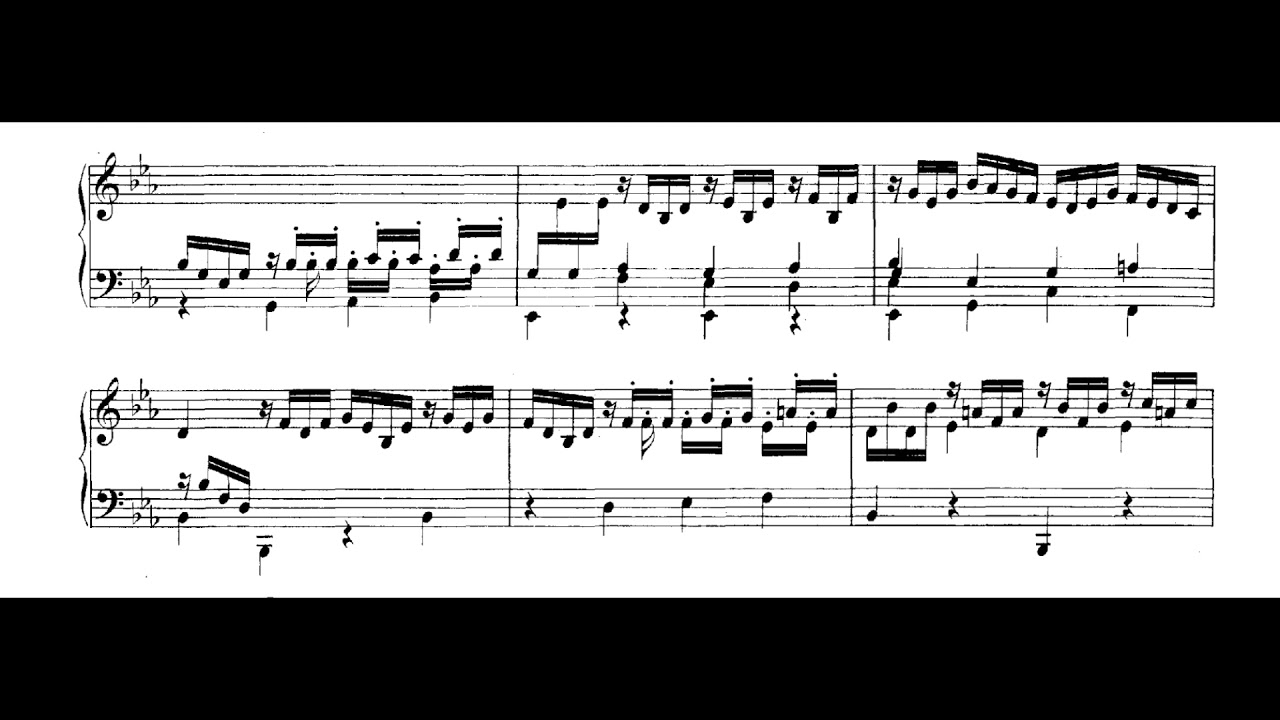
\includegraphics[width=0.48\linewidth]{pictures/youtube/2025/06/20250617_081655_youtube_001_E19gz_uAM2Q.jpg}
}
\end{center}



スヴャトスラフ・リヒテルなのか？（楽譜とピアノ演奏）


fugueで、テーマが何処に現れているか、がとてもよく分かる。特にfugueの中間部（分散和音風のところ）に、こんなにもテーマがあちらこちらに埋め込まれていたとは、初めて知りましたよ。宝探しみたいで本当に面白い。


0:00 - Prelude

\url{https://youtu.be/E19gz_uAM2Q}



2:28 - Fugue

\url{https://youtu.be/E19gz_uAM2Q?t=148s}



7:23 - Allegro

\url{https://youtu.be/E19gz_uAM2Q?t=443s}




ギターの場合には、ここまでfugueを表現できるものかどうか？

\url{https://www.facebook.com/100002225117991/posts/9582585461825529/}



あらためて、ギターでのfugueへの挑戦、決意を新たにしましたよ。現状は、fugueの前半1/3の運指を、ああでもないこうでもないと、モタモタしてみているレベル。でも、前半1/3をクリアできたら、最後の1/3もクリアできたも同然。中間部を残すだけになるから。（実は中間部が長いみたいなんだけど）

\subsection*{2025年06月17日 08:18}
\addcontentsline{toc}{subsection}{2025年06月17日 08:18}

\paragraph{リンク}
\url{https://www.guitar.jp.net/model-19th.html}

\subsection*{2025年06月17日 08:18}
\addcontentsline{toc}{subsection}{2025年06月17日 08:18}

\paragraph{リンク}
\url{https://youtu.be/ttm7Iid-dZQ}

\begin{center}
\href{https://youtu.be/ttm7Iid-dZQ}{
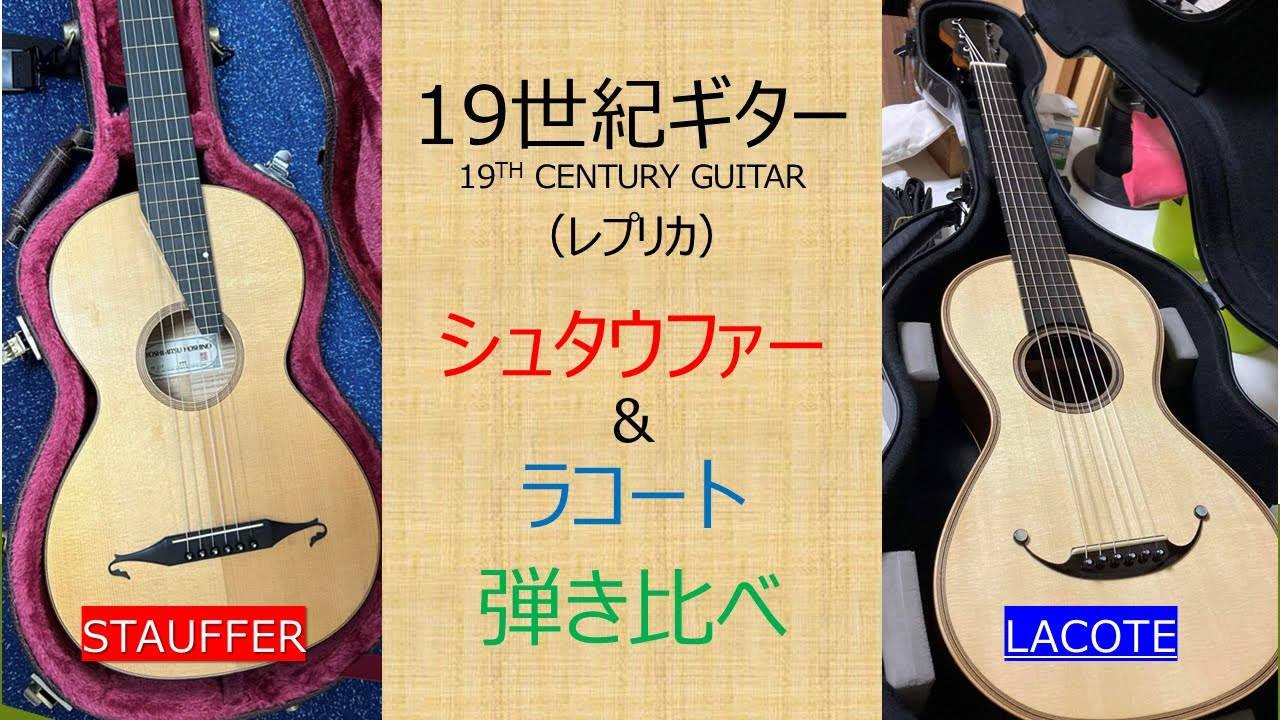
\includegraphics[width=0.48\linewidth]{pictures/youtube/2025/06/20250617_081859_youtube_001_ttm7Iid-dZQ.jpg}
}
\end{center}

\subsection*{2025年06月17日 17:24}
\addcontentsline{toc}{subsection}{2025年06月17日 17:24}

\paragraph{リンク}
\url{https://youtu.be/pYB58P3t_Hs}

\begin{center}
\href{https://youtu.be/pYB58P3t_Hs}{
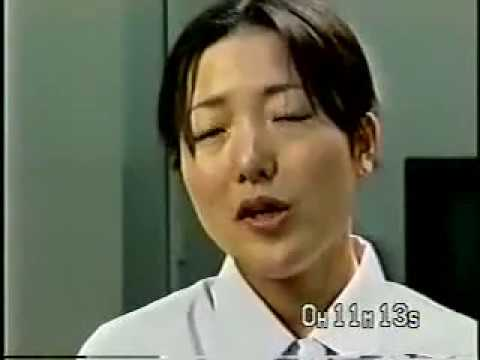
\includegraphics[width=0.48\linewidth]{pictures/youtube/2025/06/20250617_172458_youtube_001_pYB58P3t_Hs.jpg}
}
\end{center}

\subsection*{2025年06月17日 22:35}
\addcontentsline{toc}{subsection}{2025年06月17日 22:35}

\paragraph{リンク}
\url{https://youtu.be/RCX36_1wcZ0}

\begin{center}
\href{https://youtu.be/RCX36_1wcZ0}{
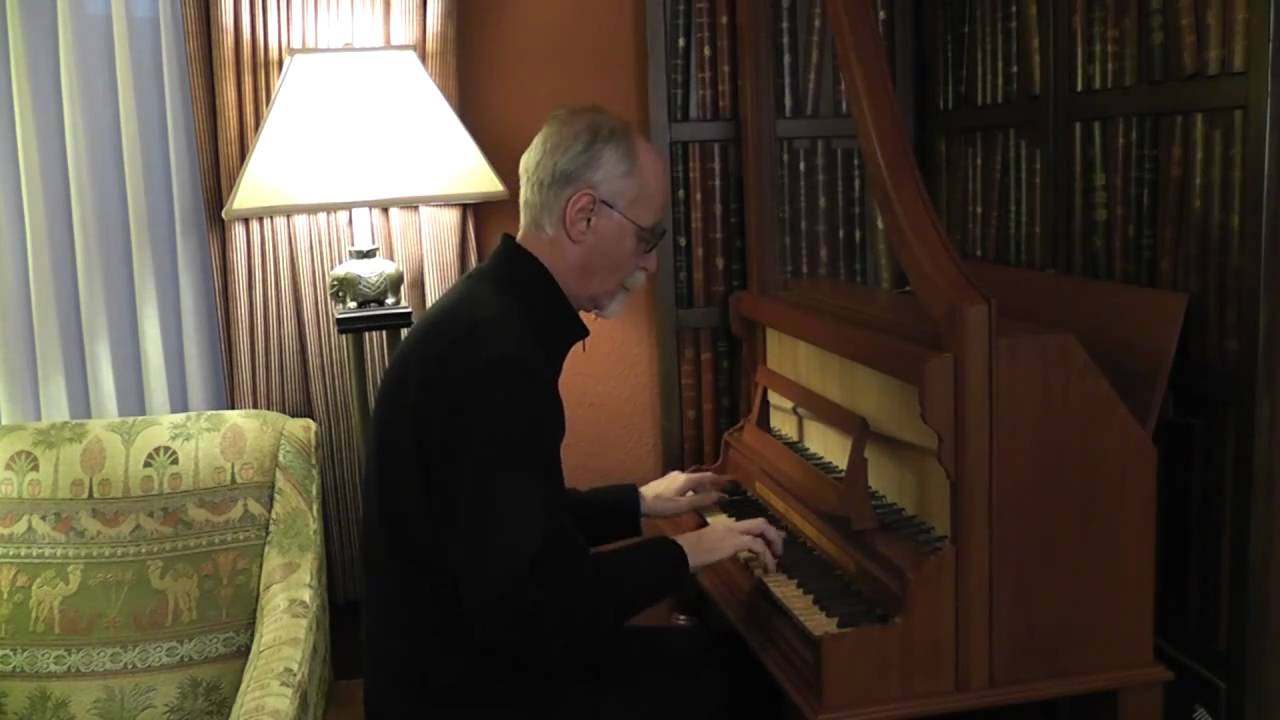
\includegraphics[width=0.48\linewidth]{pictures/youtube/2025/06/20250617_223521_youtube_001_RCX36_1wcZ0.jpg}
}
\end{center}

\subsection*{2025年06月18日 06:55}
\addcontentsline{toc}{subsection}{2025年06月18日 06:55}

\paragraph{リンク}
\url{https://youtu.be/vvr64PRMiW0}

\begin{center}
\href{https://youtu.be/vvr64PRMiW0}{
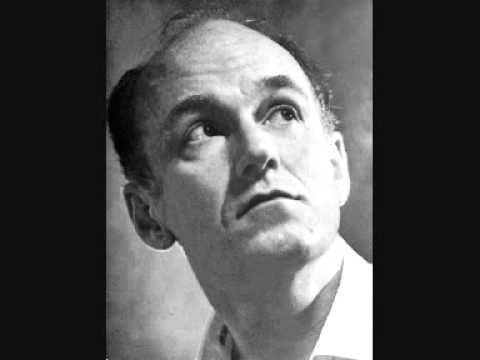
\includegraphics[width=0.48\linewidth]{pictures/youtube/2025/06/20250618_065554_youtube_001_vvr64PRMiW0.jpg}
}
\end{center}

\subsection*{2025年06月18日 13:02}
\addcontentsline{toc}{subsection}{2025年06月18日 13:02}

ChatGPTなどの用途は様々だと思いますが、私は最近fact-checkをしてみる事が多いです。


例えば、

\url{https://x.com/russiaisntenemy/status/1935005386307707124}




(１)この言説の真偽についてChatGPTに聞いてみた


ご提示の言説は、ロシアのプーチン大統領が2024年6月に行った発言を非常に正確に再現しており、ほぼ事実です。以下に詳細を整理しました。


⸻


📌 発言内容と確認できるソース


● 「イランは合意を履行してきた。アメリカが2018年に一方的に撤退し、欧州はイランに履行を要求しているのはナンセンスだ」

• 2024年6月5日、サンクトペテルブルク国際経済フォーラム（SPIEF）の場で、プーチン氏は次のように述べています：

「Иран выполнял все взятые на себя обязательства… Затем США… вышли… а европейцы продолжали требовать от Ирана… Вы уж меня… но это какой‑то бред…Что Иран должен делать?»

また英訳の報道でも同様の内容が公開されています：

“The United States unilaterally decided to withdraw… Europeans continue to demand that Iran fulfills its obligations… Forgive me, but that’s nonsense…”


これらの引用から、ユーザーの提示した英語スクリプトは非常に忠実に再現されており、実際の発言と一致しています。


⸻


● 「“I’m sorry, but this is just nonsense… Why the hell should Iran have done that?”（“Forgive my language, it sounds harsh in Russian…”）の部分も一致


SPIEFでの発言中に、プーチン氏自身が「…по‑русски звучит грубовато…」「…какого хрена‑то иранцы?…」と、ロシア語で語気を強めています  。


⸻


✅ 総合評価

• 真実性：高い

• 提示された英語の発言文は、実際の発言に忠実な引用であり、事実に基づいています。


(２)次に、発言された内容について、引き続きChatGPTに聞いてみた


とても重要なご質問です。「プーチン大統領がそのように発言した」ことと、その発言の**内容（事実性）**が信頼できるかどうかは、別問題です。以下に分解して検証します。


（途中省略ー結論は添付画像の通り）

\paragraph{写真}
\begin{center}
\begin{minipage}{0.48\linewidth}
\centering
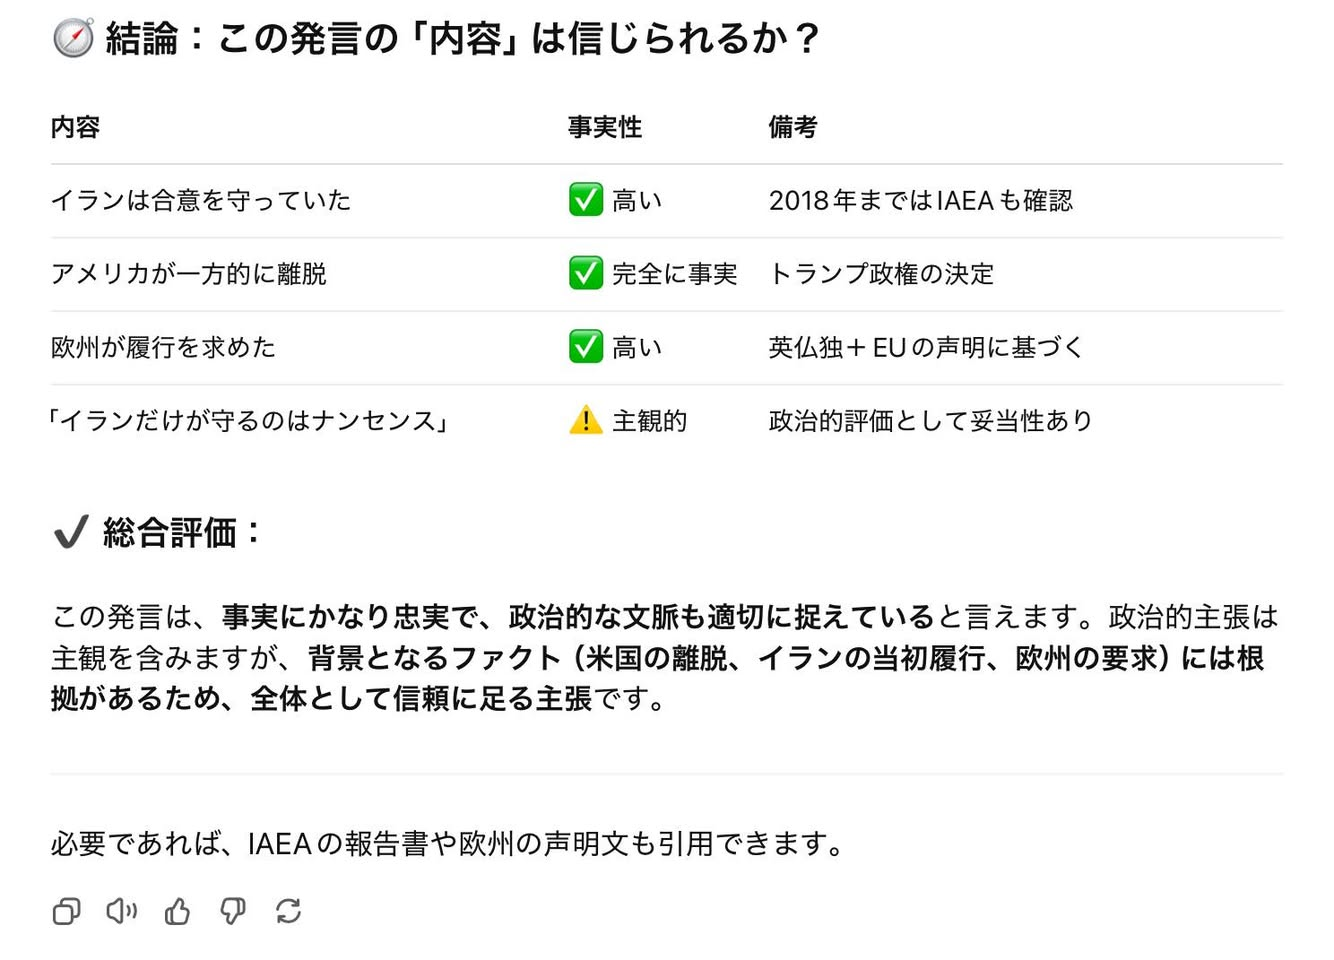
\includegraphics[width=\linewidth]{pictures/2025/06/20250618_130241_001.jpg}
\end{minipage}
\end{center}

\subsection*{2025年06月18日 13:35}
\addcontentsline{toc}{subsection}{2025年06月18日 13:35}

石破さんのお気持ち、お察しします。

自分も、これと似た状況にあったら、きっと同じ様な事になるんじゃないかと思うから。（英検準一級対策にでも取り組んでみようかな）

\paragraph{写真}
\begin{center}
\begin{minipage}{0.48\linewidth}
\centering
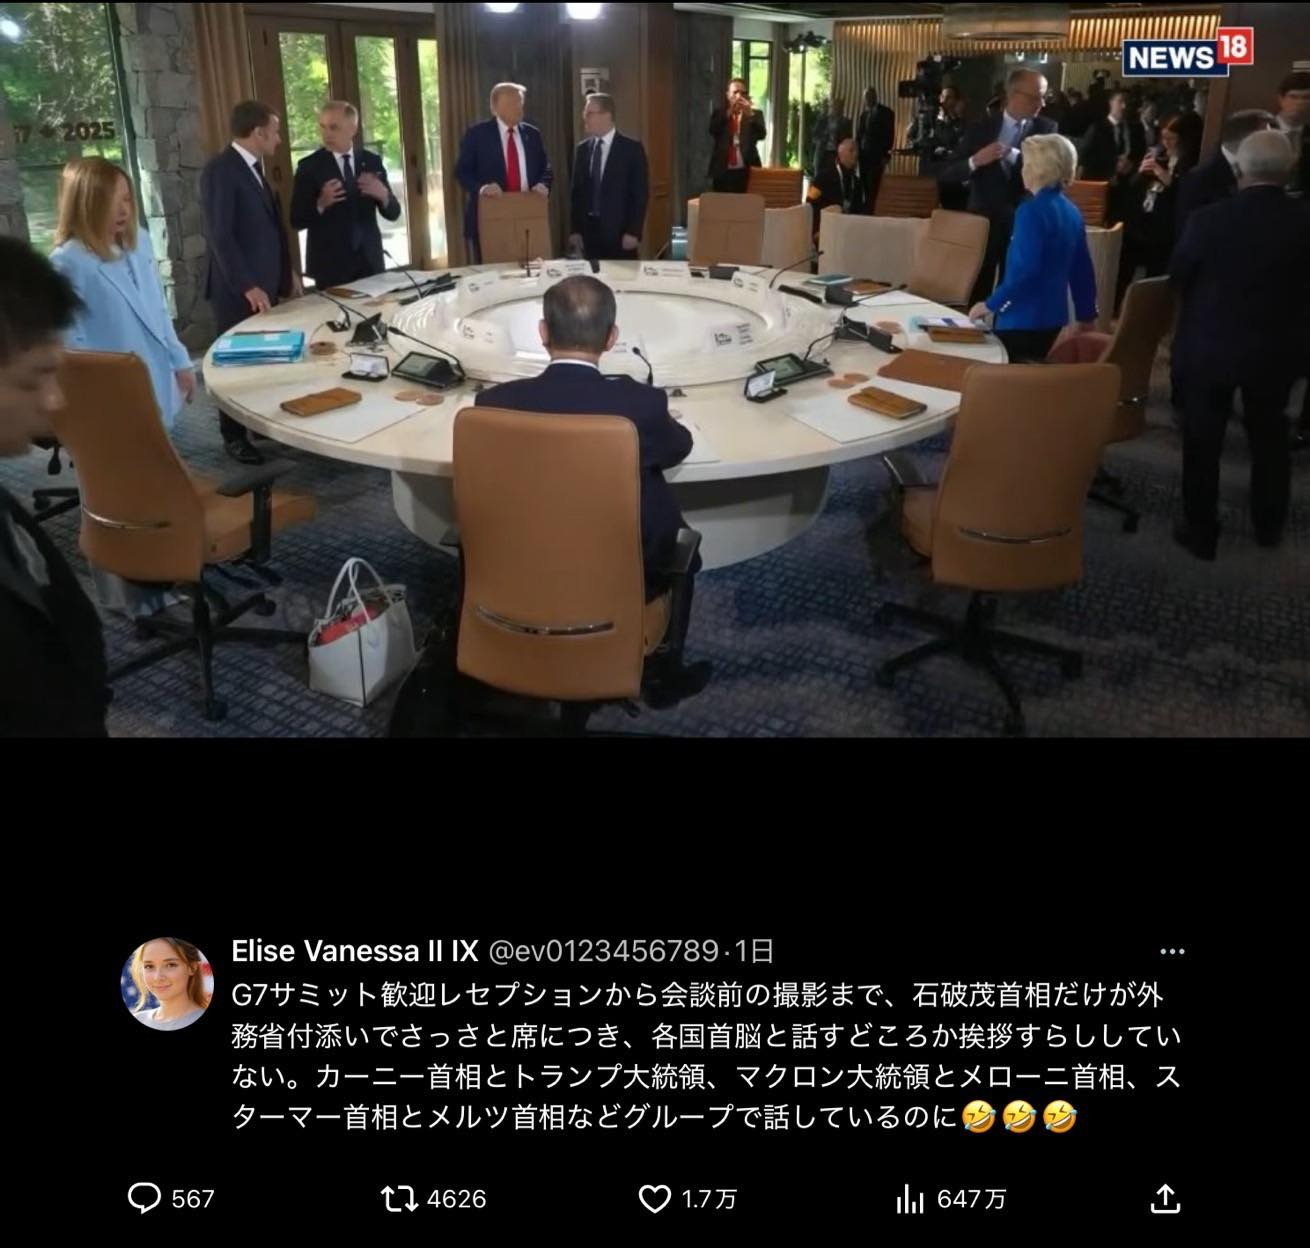
\includegraphics[width=\linewidth]{pictures/2025/06/20250618_133518_001.jpg}
\end{minipage}
\hfill
\begin{minipage}{0.48\linewidth}
\centering
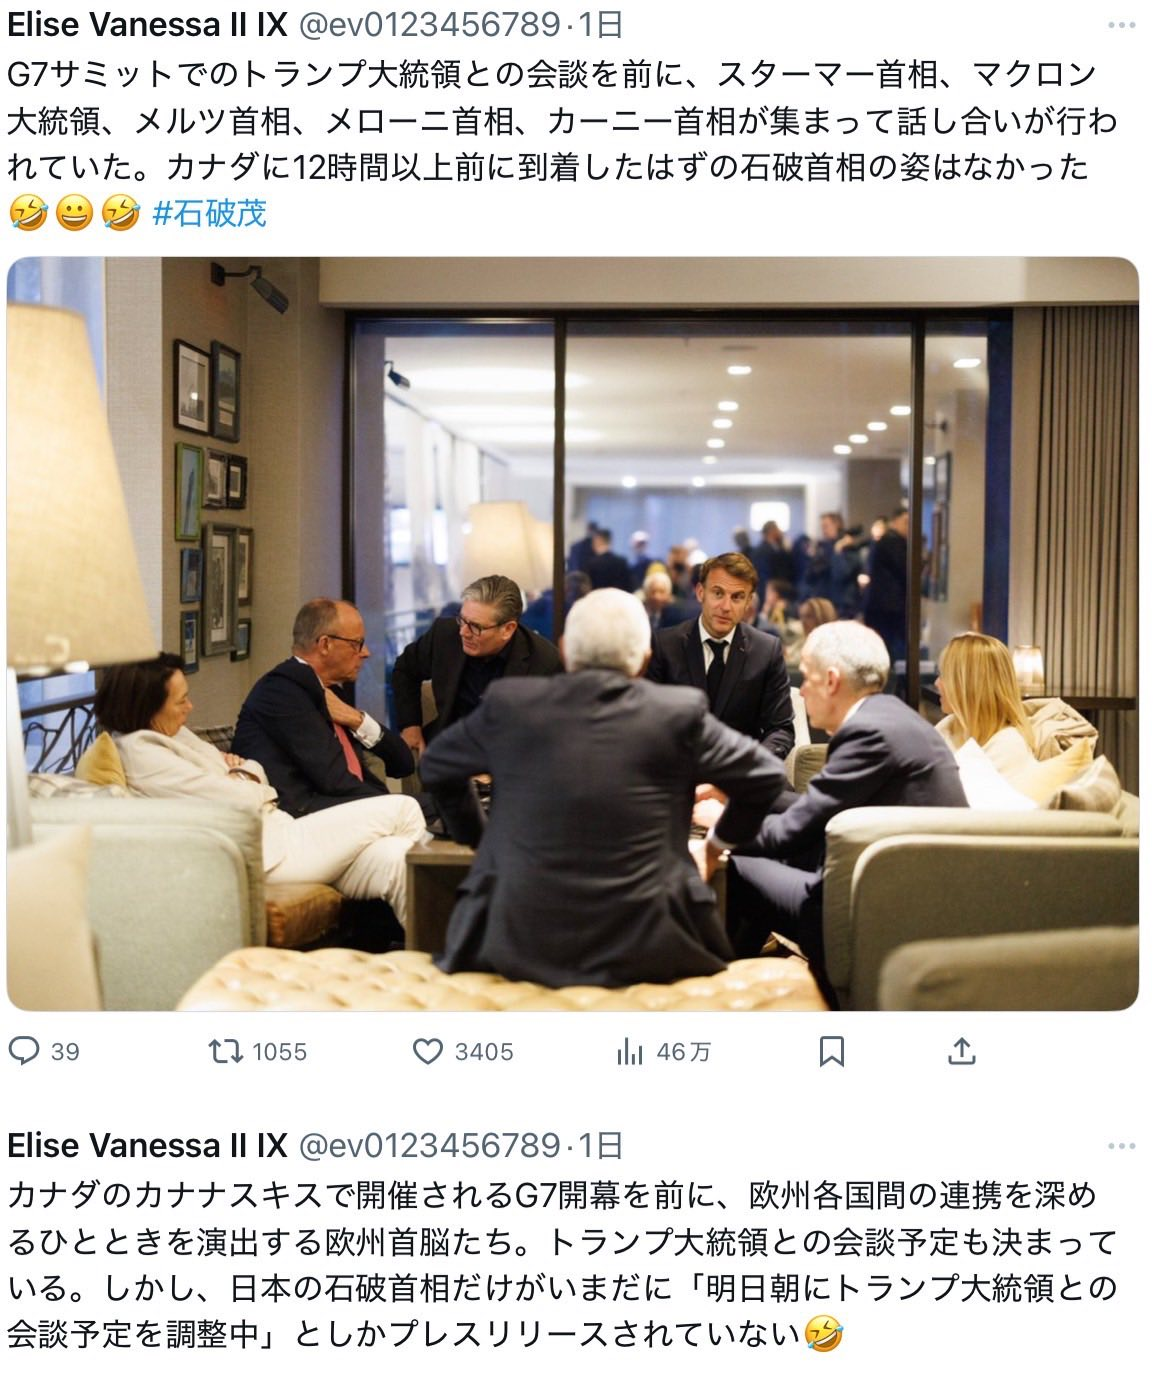
\includegraphics[width=\linewidth]{pictures/2025/06/20250618_133518_002.jpg}
\end{minipage}
\end{center}

\subsection*{2025年06月18日 20:20}
\addcontentsline{toc}{subsection}{2025年06月18日 20:20}

\url{https://youtu.be/p0jjxqpC0aY}

\begin{center}
\href{https://youtu.be/p0jjxqpC0aY}{
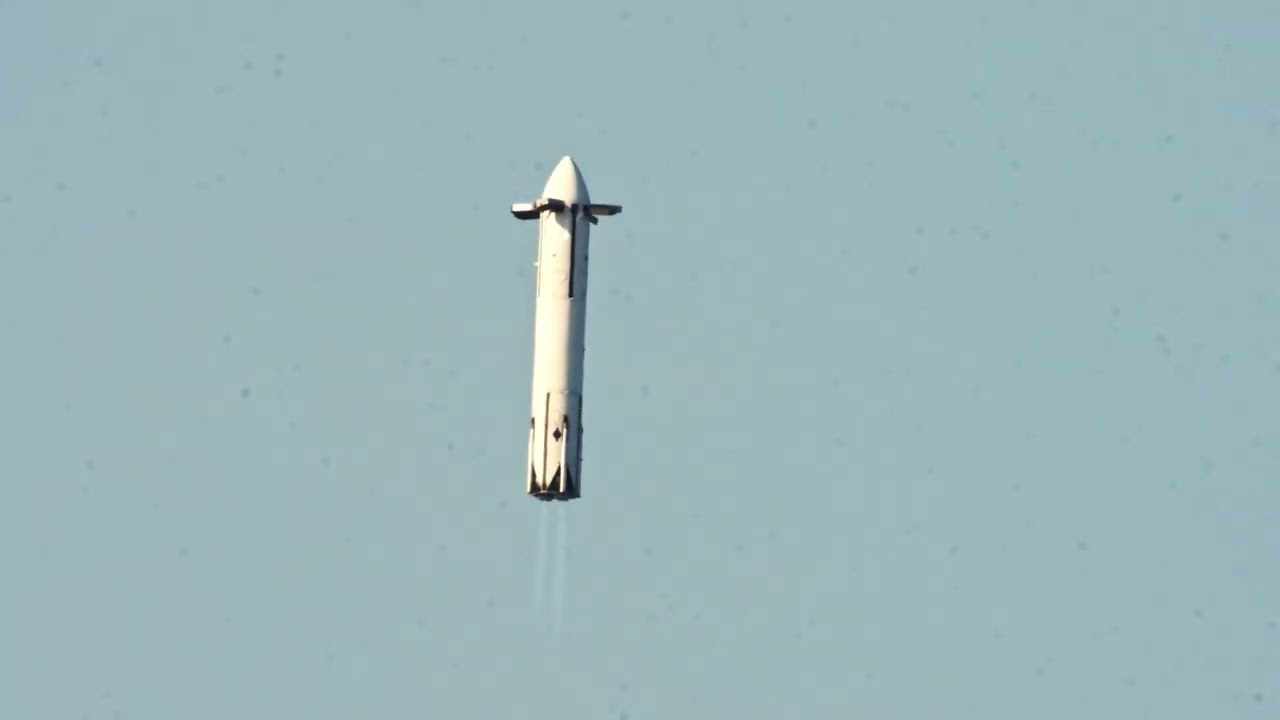
\includegraphics[width=0.48\linewidth]{pictures/youtube/2025/06/20250618_202024_youtube_001_p0jjxqpC0aY.jpg}
}
\end{center}




ホンダがこれを成功させてくれたのは嬉しい事だ。

X社の物よりずっと安定して美しいのではないかと言う気がする。（勿論ひいき目なのかもしれないですけど）

次は、降りてくる所をハシで摘んで（挟んで）みせてほしい。

\subsection*{2025年06月18日 20:56}
\addcontentsline{toc}{subsection}{2025年06月18日 20:56}

\paragraph{リンク}
\url{https://youtu.be/FTztTK7n27g}

\begin{center}
\href{https://youtu.be/FTztTK7n27g}{
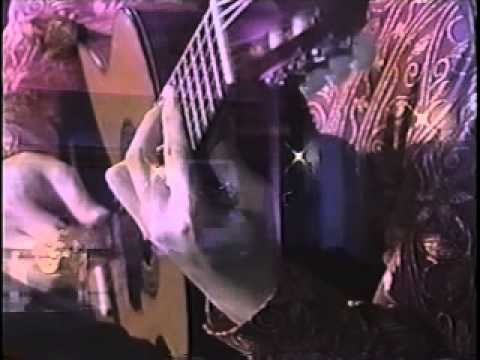
\includegraphics[width=0.48\linewidth]{pictures/youtube/2025/06/20250618_205619_youtube_001_FTztTK7n27g.jpg}
}
\end{center}

\subsection*{2025年06月19日 18:15}
\addcontentsline{toc}{subsection}{2025年06月19日 18:15}

メリーポピンズ

\url{https://youtu.be/oQPJvzhqr4U}

\begin{center}
\href{https://youtu.be/oQPJvzhqr4U}{
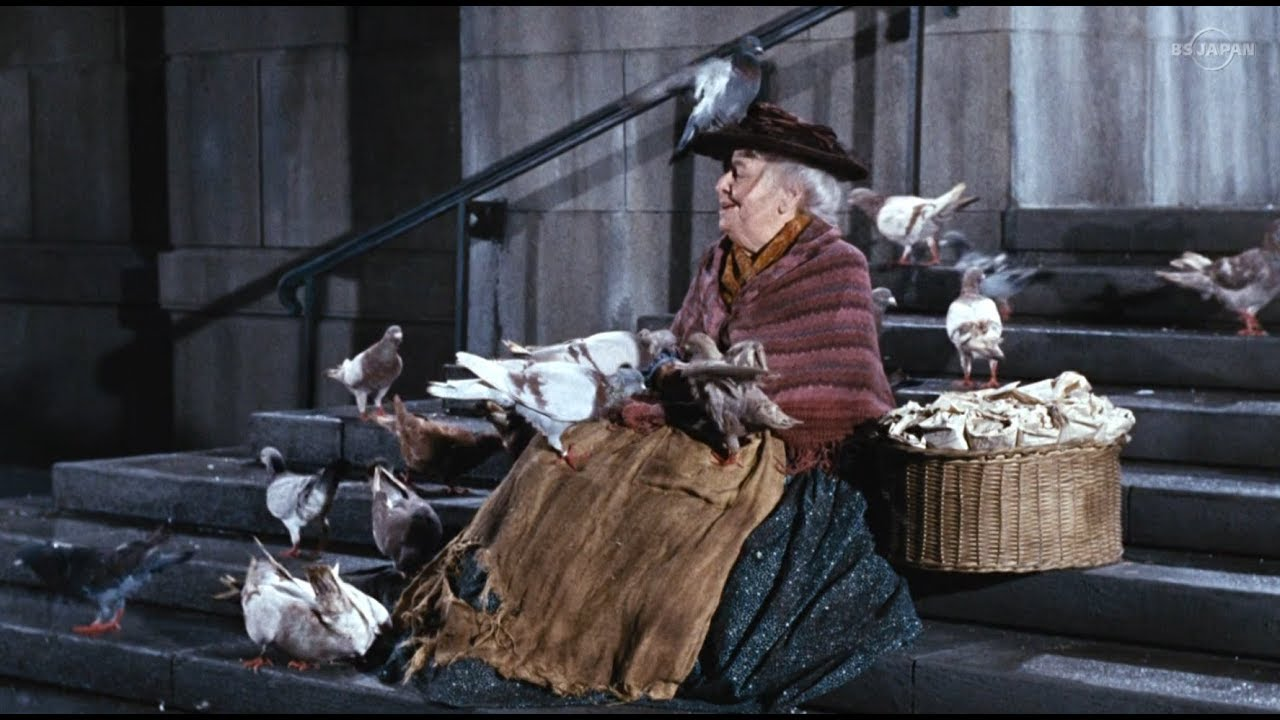
\includegraphics[width=0.48\linewidth]{pictures/youtube/2025/06/20250619_181525_youtube_001_oQPJvzhqr4U.jpg}
}
\end{center}



\url{https://youtu.be/jENfyP5Eqjw}

\begin{center}
\href{https://youtu.be/jENfyP5Eqjw}{
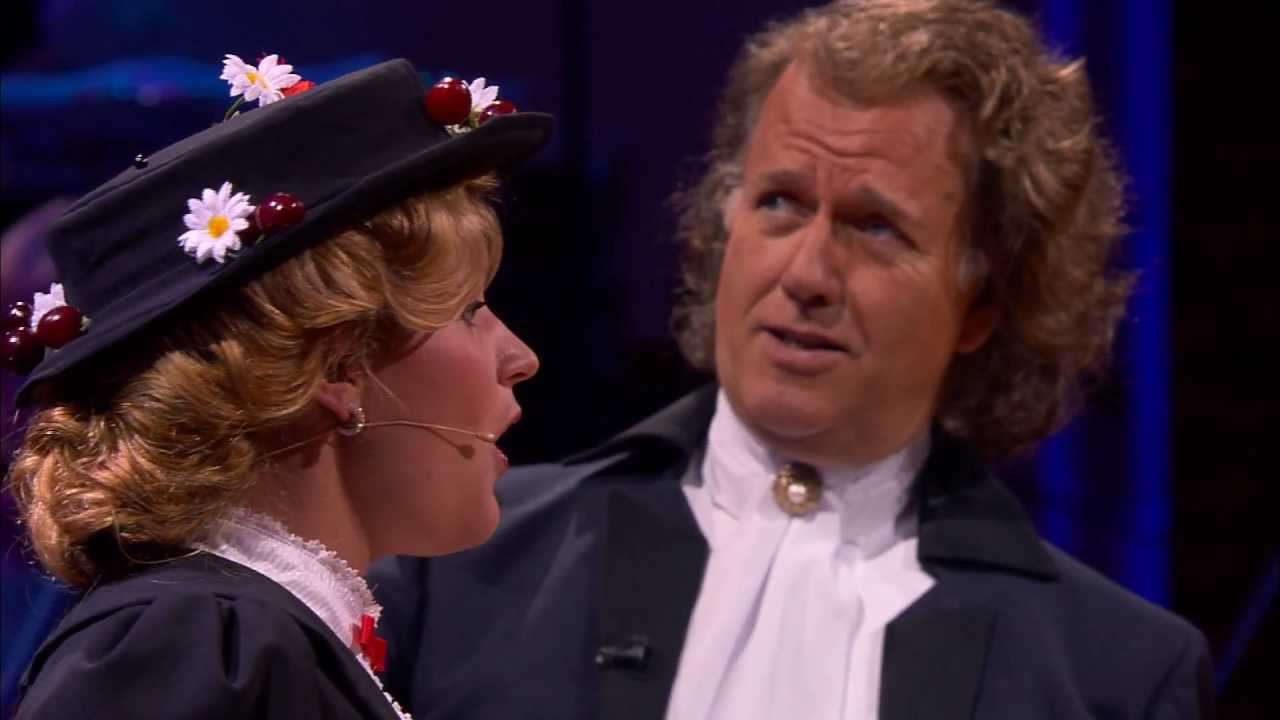
\includegraphics[width=0.48\linewidth]{pictures/youtube/2025/06/20250619_181525_youtube_002_jENfyP5Eqjw.jpg}
}
\end{center}




Though her words are simple and few

"Listen, listen", she's calling to you

"Feed the birds, tuppence a bag

Tuppence, tuppence, tuppence a bag"

\subsection*{2025年06月20日 03:08}
\addcontentsline{toc}{subsection}{2025年06月20日 03:08}

\paragraph{リンク}
\url{https://youtu.be/AGDi8dDTSx8}

\begin{center}
\href{https://youtu.be/AGDi8dDTSx8}{
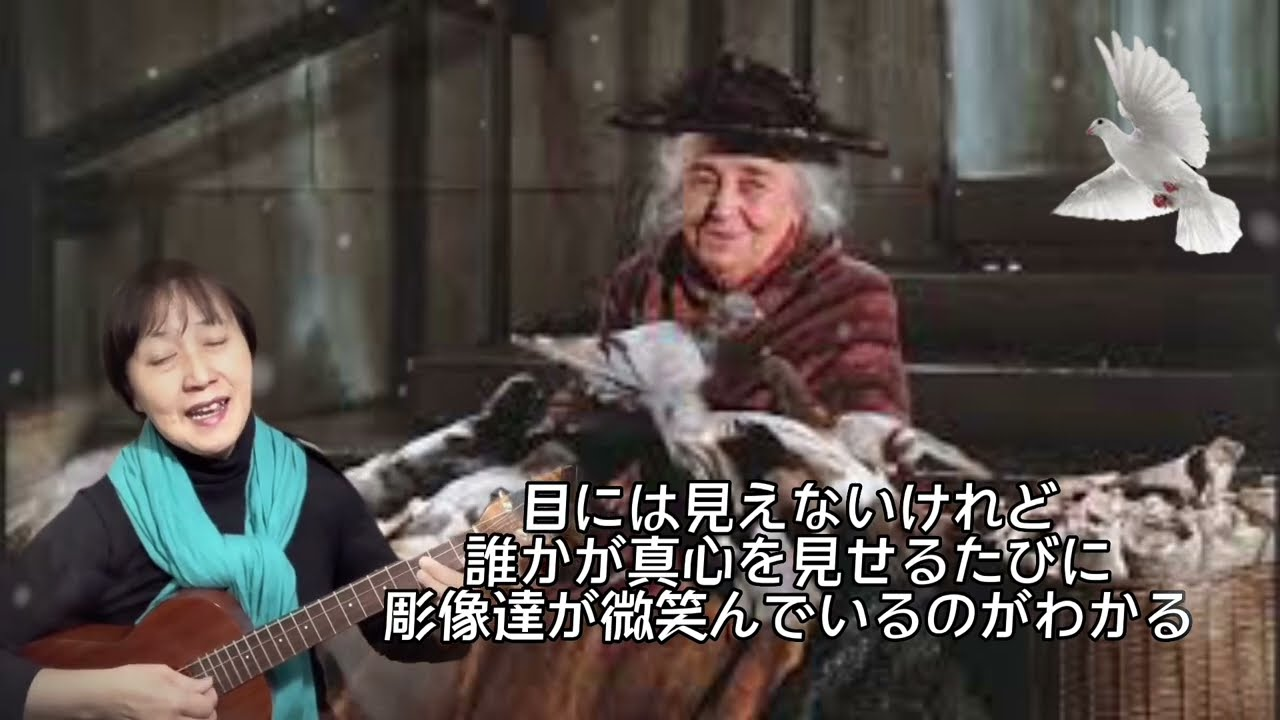
\includegraphics[width=0.48\linewidth]{pictures/youtube/2025/06/20250620_030827_youtube_001_AGDi8dDTSx8.jpg}
}
\end{center}

\subsection*{2025年06月20日 03:42}
\addcontentsline{toc}{subsection}{2025年06月20日 03:42}

\paragraph{リンク}
\url{https://youtu.be/EkOaPi6nFrI}

\begin{center}
\href{https://youtu.be/EkOaPi6nFrI}{
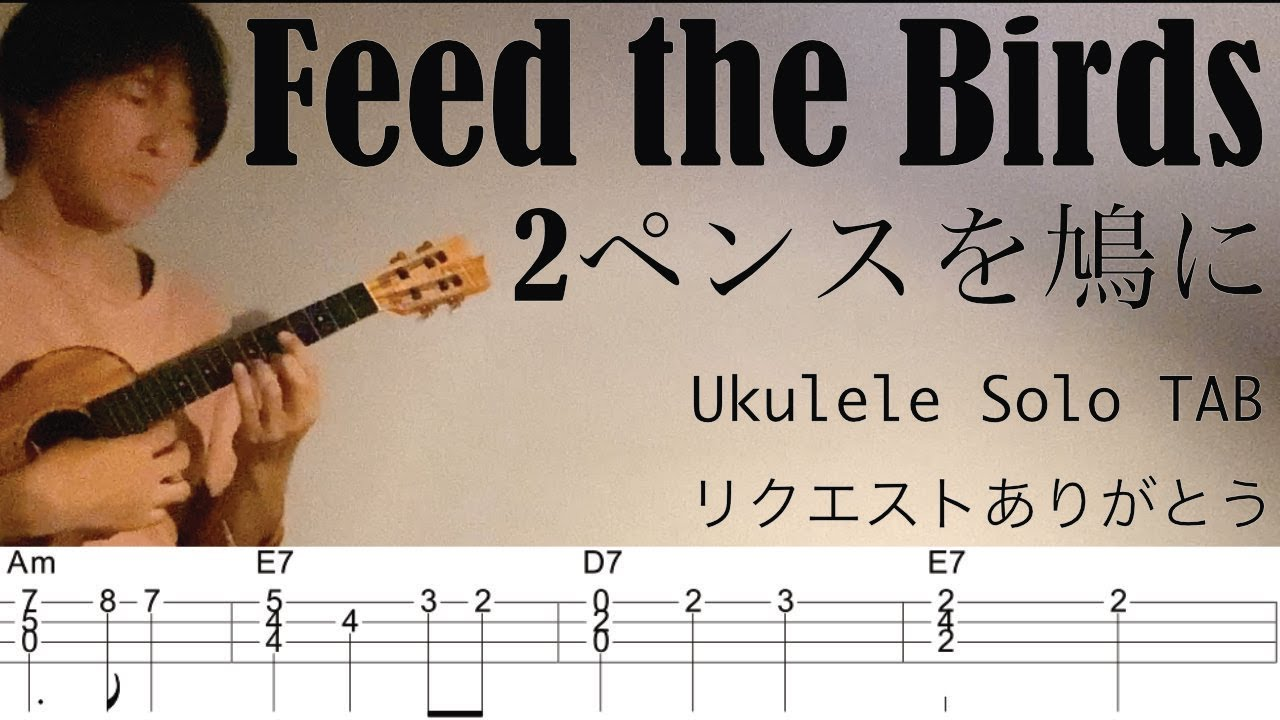
\includegraphics[width=0.48\linewidth]{pictures/youtube/2025/06/20250620_034217_youtube_001_EkOaPi6nFrI.jpg}
}
\end{center}

\subsection*{2025年06月20日 04:02}
\addcontentsline{toc}{subsection}{2025年06月20日 04:02}

\paragraph{リンク}
\url{https://youtu.be/jENfyP5Eqjw}

\begin{center}
\href{https://youtu.be/jENfyP5Eqjw}{
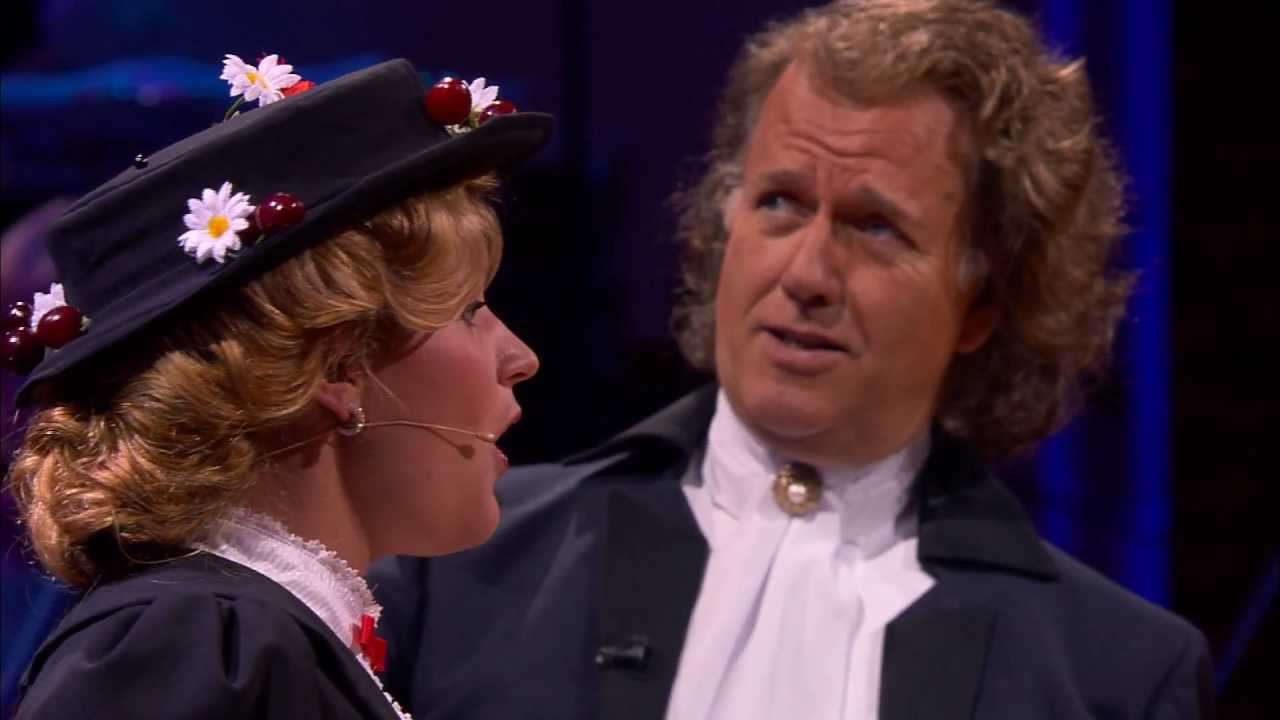
\includegraphics[width=0.48\linewidth]{pictures/youtube/2025/06/20250620_040229_youtube_001_jENfyP5Eqjw.jpg}
}
\end{center}

\subsection*{2025年06月20日 04:04}
\addcontentsline{toc}{subsection}{2025年06月20日 04:04}

\paragraph{リンク}
\url{https://youtu.be/S2VVjNvhlms}

\begin{center}
\href{https://youtu.be/S2VVjNvhlms}{
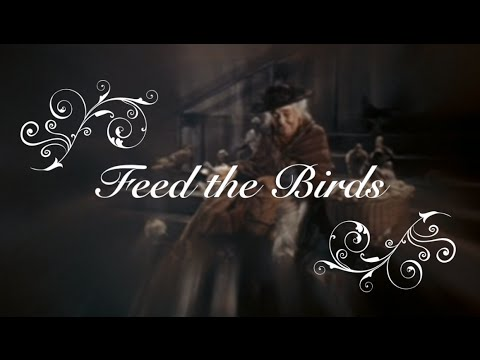
\includegraphics[width=0.48\linewidth]{pictures/youtube/2025/06/20250620_040433_youtube_001_S2VVjNvhlms.jpg}
}
\end{center}

\subsection*{2025年06月20日 04:48}
\addcontentsline{toc}{subsection}{2025年06月20日 04:48}

\paragraph{リンク}
\url{https://youtu.be/IWH3Hmsr5fM}

\begin{center}
\href{https://youtu.be/IWH3Hmsr5fM}{
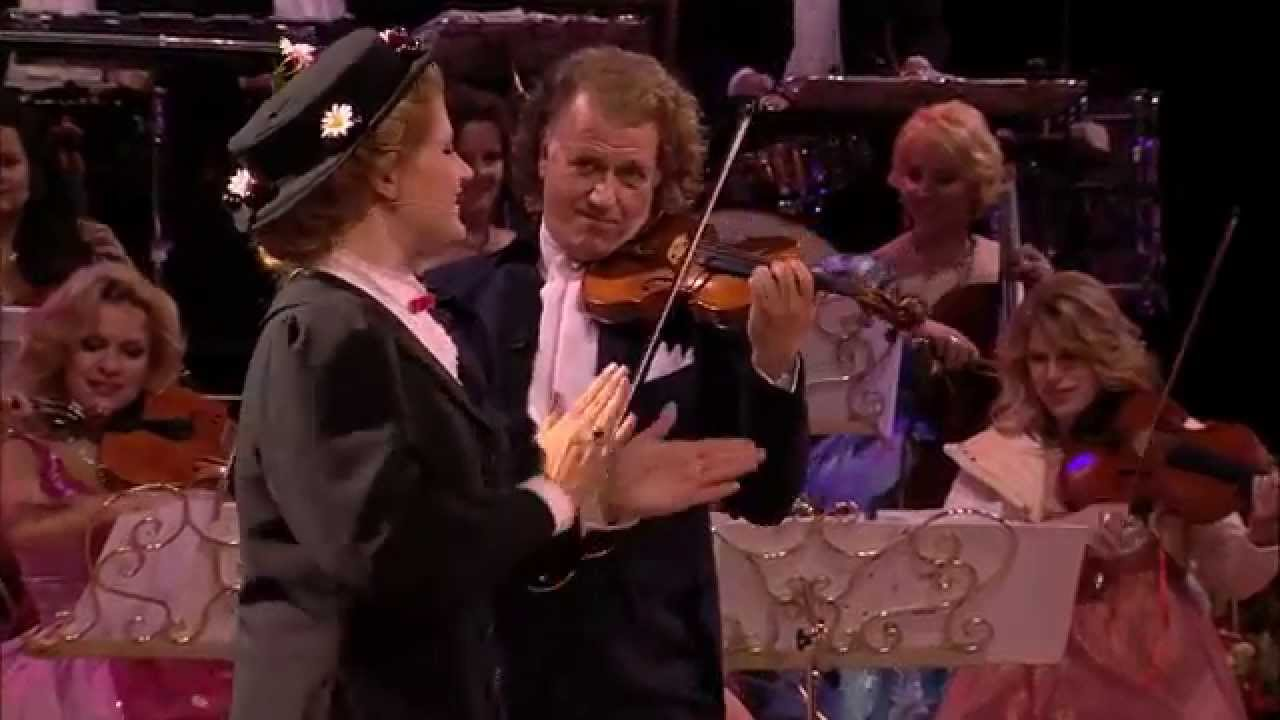
\includegraphics[width=0.48\linewidth]{pictures/youtube/2025/06/20250620_044803_youtube_001_IWH3Hmsr5fM.jpg}
}
\end{center}

\subsection*{2025年06月21日 00:59}
\addcontentsline{toc}{subsection}{2025年06月21日 00:59}

\paragraph{リンク}
\url{https://www.kyotoprize.org/laureates/shun-ichi_amari/}

\subsection*{2025年06月21日 04:47}
\addcontentsline{toc}{subsection}{2025年06月21日 04:47}

ChatGPTですが、あれやこれやと遊んでみています。添付は、元ネタにした写真と、そこから生成された画像です。


最初は(１)スナフキンの帽子と(２)トラベルソを吹いてる事を要求したものです。途中でカメラとバッグはいらないと言ったら、なぜかスナフキン風の帽子がベレー帽に変わって爺さん風の画像になって、背景も違った画像になりました。また、最後までトラベルソのディテールは描かれませんでしたね。あんまりよく知らないのかな？或いは、日本的な背景には西洋の横笛より日本風の横笛が合うというイメージが作図に影響したものかもしれません。


笛を吹いているものでは、比較的若い感じ (\textasciicircum{}\textasciicircum{};; の画像を選ぶ事にしましたが、爺さん風の画像も悪くない気がしたので、トラベルソをギターに代えて作図してくれるように要求してみました。ギターのディテールについてはそれなりによく描かれているようです。（クラシックギターがアコースティックギターや三味線にならなくてよかったよ）

\paragraph{写真}
\begin{center}
\begin{minipage}{0.48\linewidth}
\centering
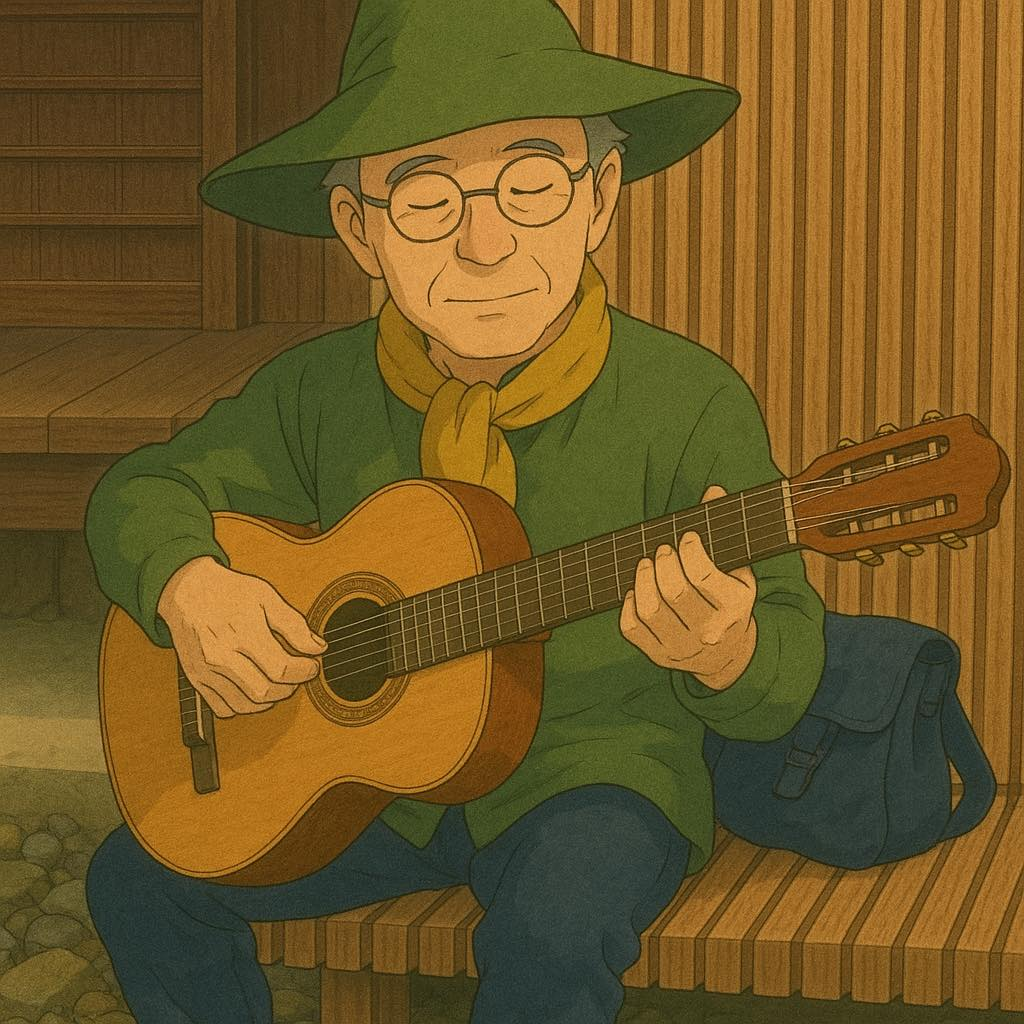
\includegraphics[width=\linewidth]{pictures/2025/06/20250621_044730_001.jpg}
\end{minipage}
\hfill
\begin{minipage}{0.48\linewidth}
\centering
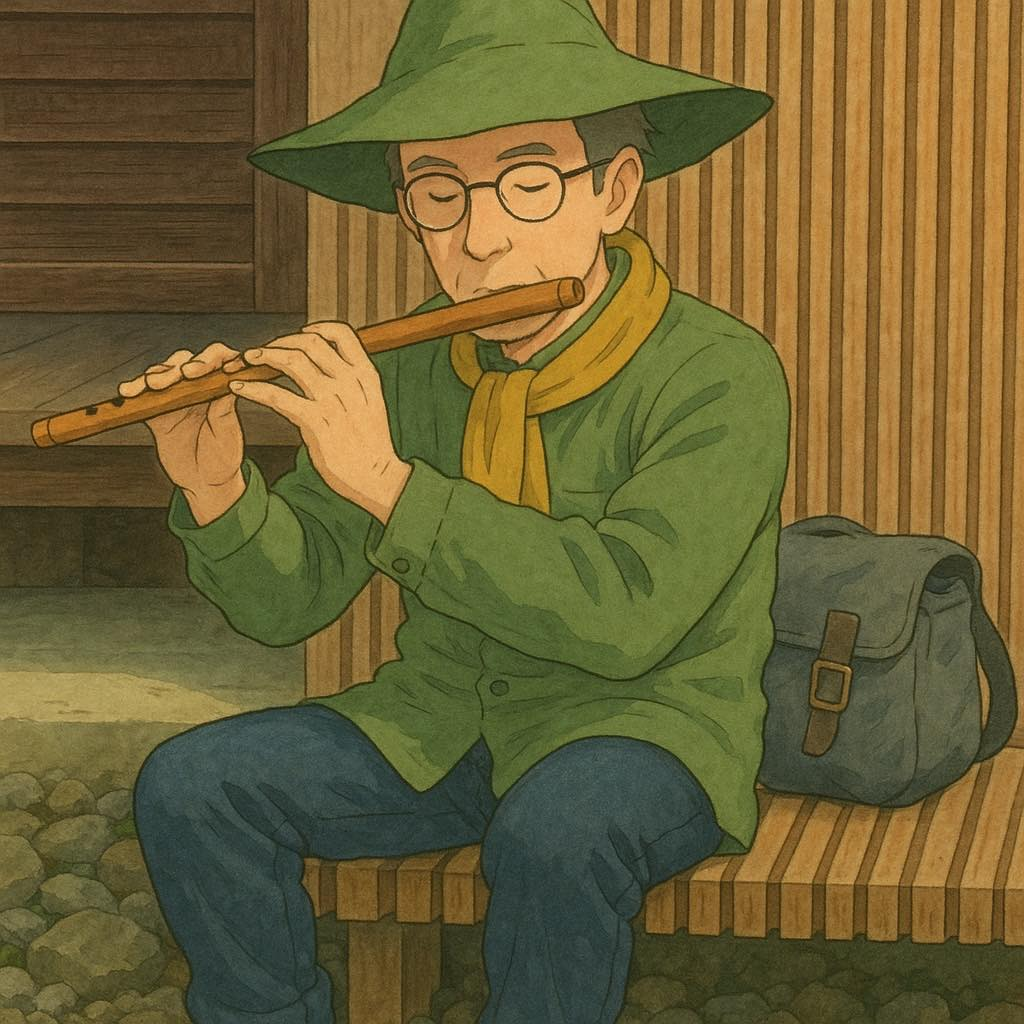
\includegraphics[width=\linewidth]{pictures/2025/06/20250621_044730_002.jpg}
\end{minipage}
\end{center}

\begin{center}
\begin{minipage}{0.48\linewidth}
\centering
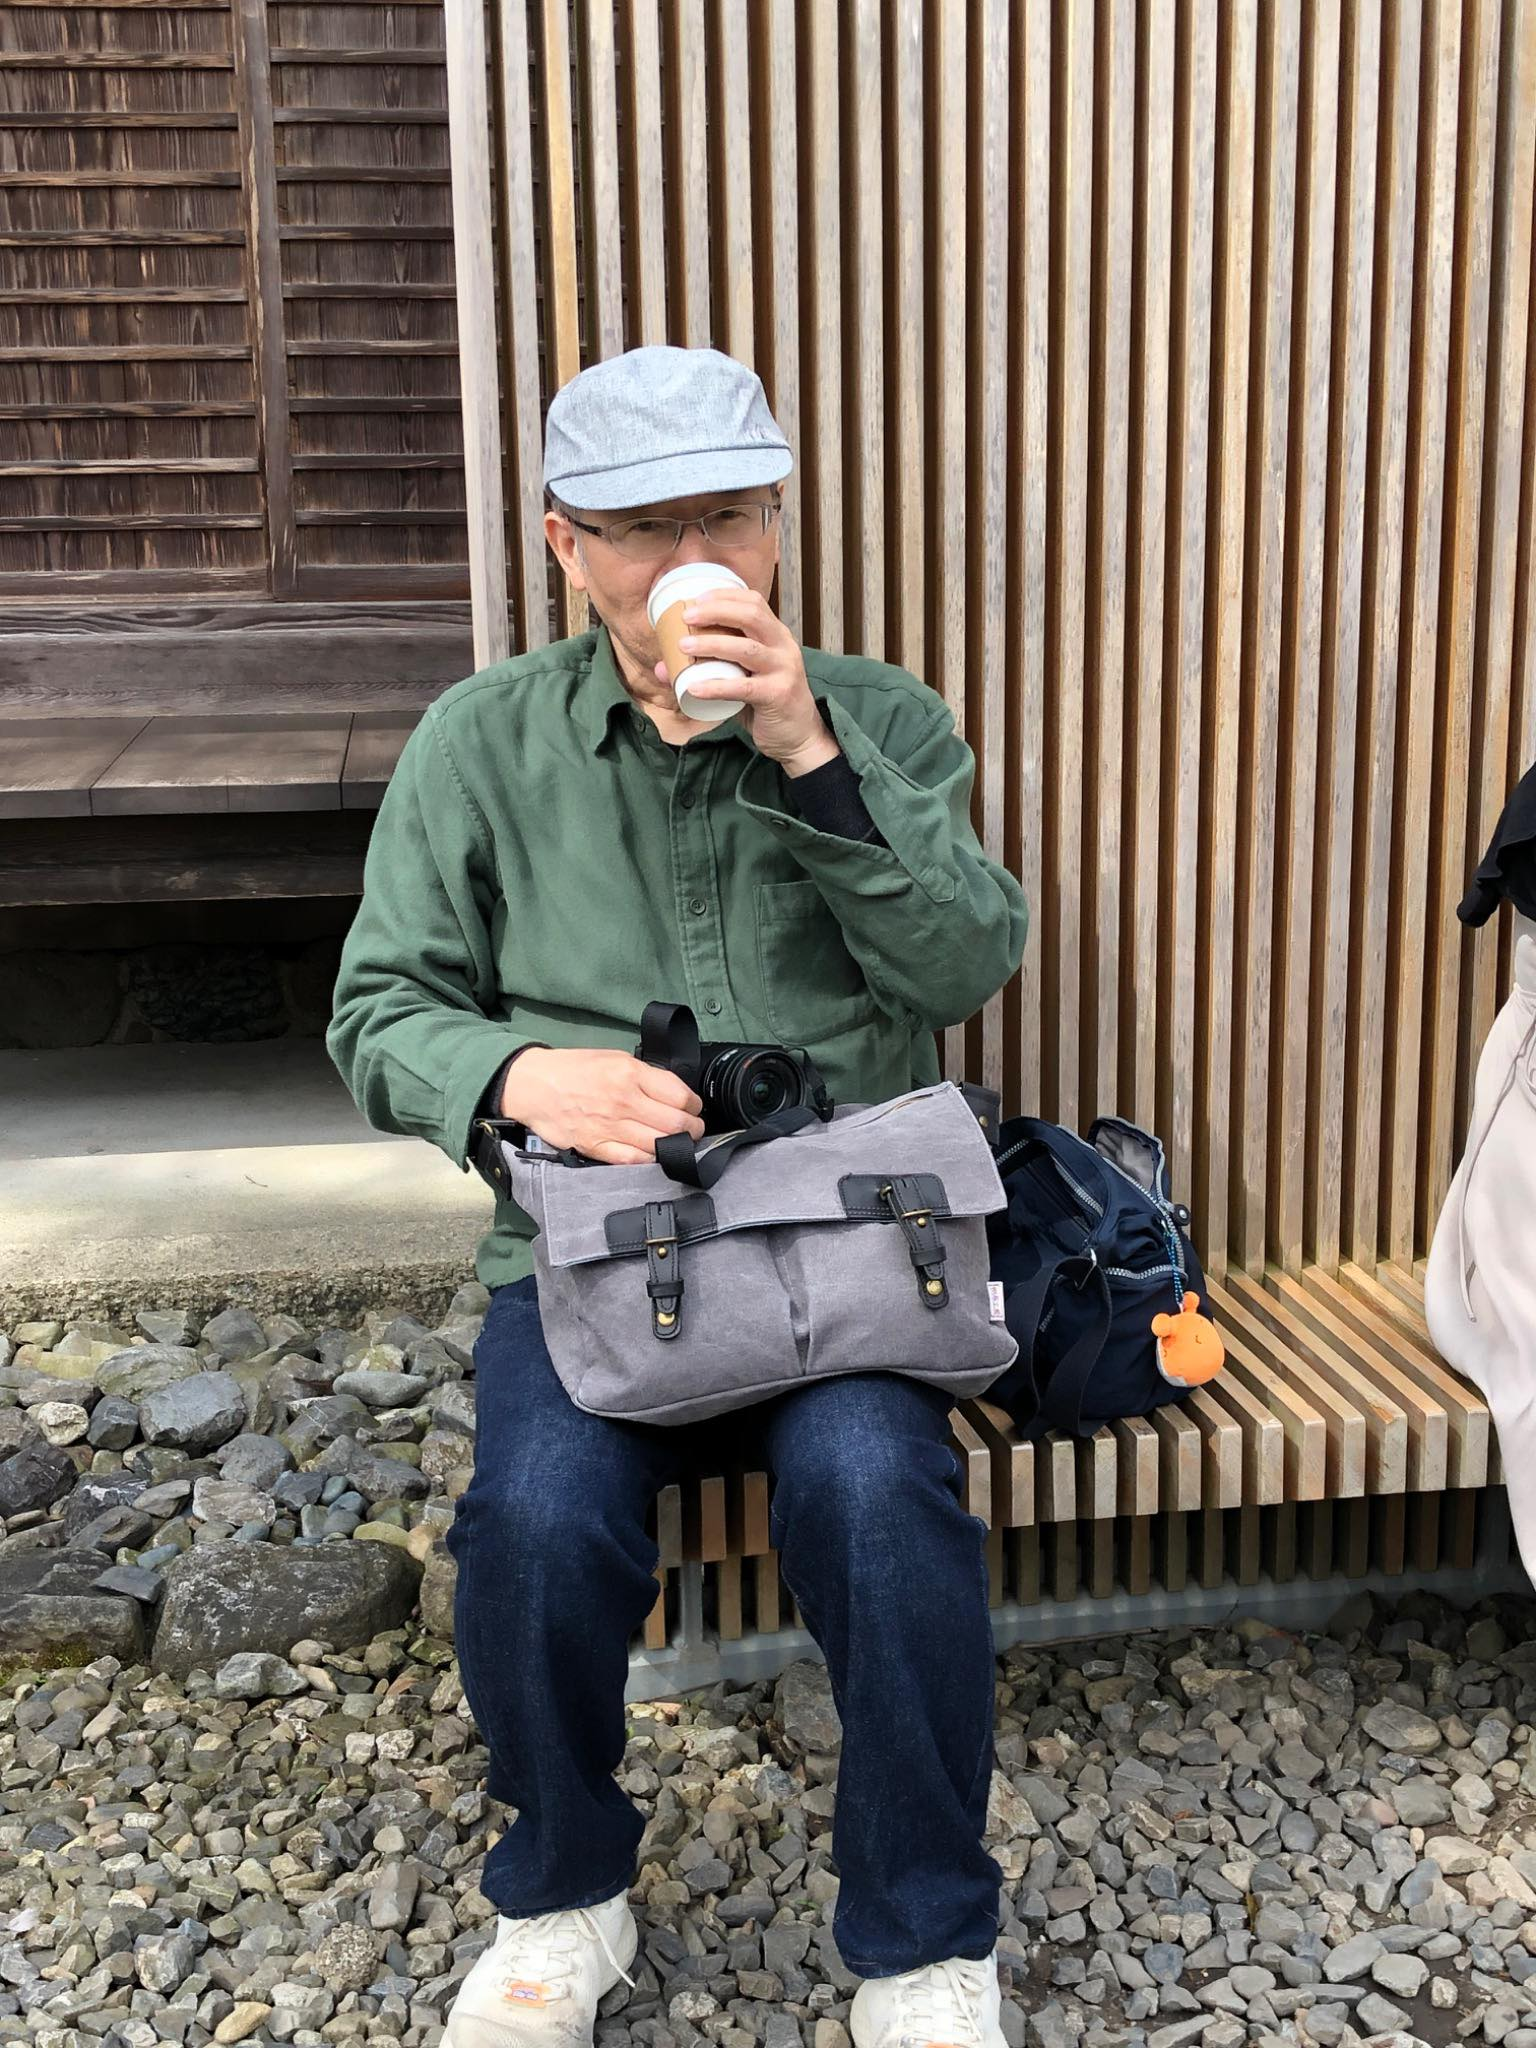
\includegraphics[width=\linewidth]{pictures/2025/06/20250621_044730_003.jpg}
\end{minipage}
\end{center}

\subsection*{2025年06月21日 11:04}
\addcontentsline{toc}{subsection}{2025年06月21日 11:04}

自分が、西田幾多郎に関する書を繰り返し読む（参照する）気になるとは、全く予想だにできなかった事だ。


理解できると言ってはおこがましいし、そもそも西田幾多郎とその哲学について私が語れるものなど皆無なのだが、「なるほど」とか「なんとなくその気持ち分かる」といった、「何か腑に落ちる様な気にさせる言葉」が随所に（←これは言い過ぎ。所々に、が正しい。）現れるものだから、「あれは何処に書かれていたっけ」と読み直す事になってしまう。よく見直す事になる本は、主に下の二冊（添付画像）だ。（「善の研究」の方は部分的にしか読めていない(-｡-;）

\paragraph{写真}
\begin{center}
\begin{minipage}{0.48\linewidth}
\centering
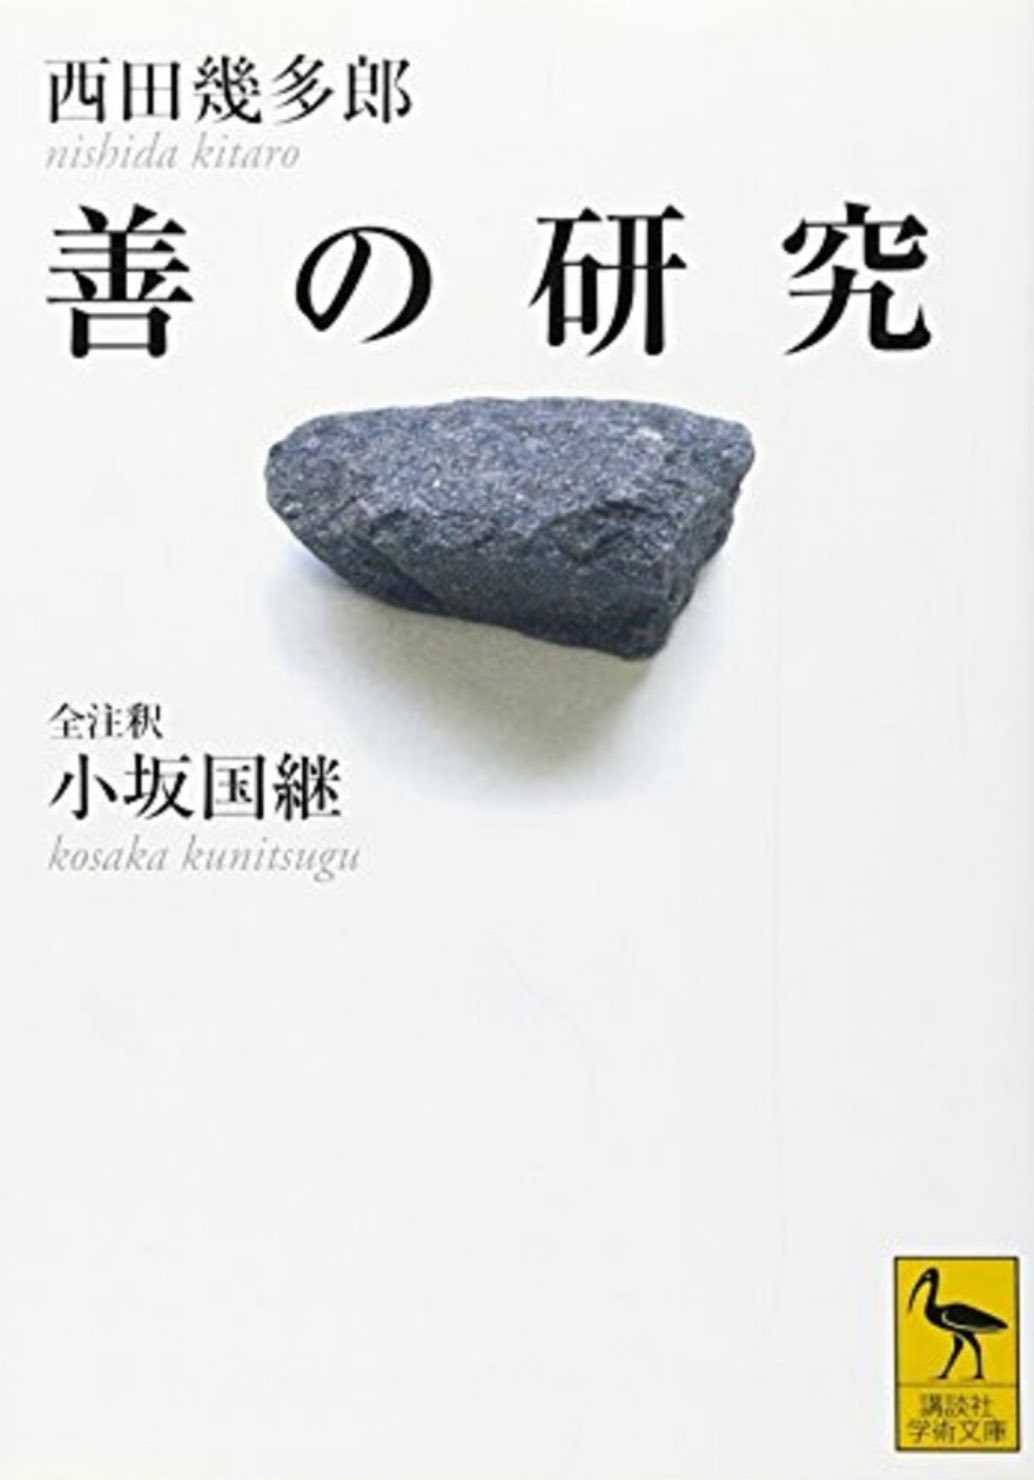
\includegraphics[width=\linewidth]{pictures/2025/06/20250621_110401_001.jpg}
\end{minipage}
\hfill
\begin{minipage}{0.48\linewidth}
\centering
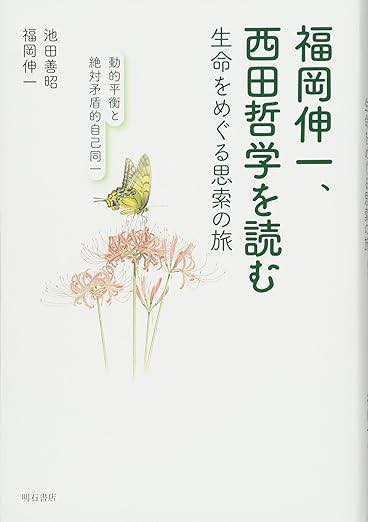
\includegraphics[width=\linewidth]{pictures/2025/06/20250621_110401_002.jpg}
\end{minipage}
\end{center}

\subsection*{2025年06月23日 01:17}
\addcontentsline{toc}{subsection}{2025年06月23日 01:17}

「Smoke gets in your eyes（煙が目にしみる)」（←名訳やなぁ）

作曲：Jerome Kern

作詞：Otto Harbach

ギター編：J.W.Duarte


\url{https://youtu.be/kisFJNzu8x4}

\begin{center}
\href{https://youtu.be/kisFJNzu8x4}{
\includegraphics[width=0.48\linewidth]{pictures/youtube/2025/06/20250623_011738_youtube_001_kisFJNzu8x4.jpg}
}
\end{center}




高音部で鳴るナイロン弦の単音（ビブラート付き）が何とも魅力的に響いています。グリッサンドも効果的です。残念だけどこの楽譜は（現在）手に入らないみたいです。（他の方の編曲なら手に入りますが）


（その後）

この楽譜のPDFがネット上に落ちていました。(.ru はロシアのドメインか？)

\url{https://ehgdae.ru/base/download/?notes=3924&sess=100901}



キリ・テ・カナワのCDアルバム「Kiri sings Kern(ジェローム・カーン名作集)」の中で歌われている曲の多くが、この楽譜でギター独奏用に編曲されて載っている。この楽譜を見つけることができてとても嬉しい。この楽譜を全曲録音しているギターリストはいないんだろうか？


===

続きはここ↓

\url{https://m.facebook.com/story.php?story_fbid=10092725310811539&id=100002225117991}



\subsection*{2025年06月23日 12:52}
\addcontentsline{toc}{subsection}{2025年06月23日 12:52}

戦後80年の沖縄慰霊の日を見ていたら、子供たちが歌っていたので、何だか聞きたくなりました。

\paragraph{リンク}
\url{https://youtu.be/pD-ExzvMe7U}

\begin{center}
\href{https://youtu.be/pD-ExzvMe7U}{
\includegraphics[width=0.48\linewidth]{pictures/youtube/2025/06/20250623_125215_youtube_001_pD-ExzvMe7U.jpg}
}
\end{center}

\subsection*{2025年06月23日 15:09}
\addcontentsline{toc}{subsection}{2025年06月23日 15:09}

\url{https://www.asahi.com/articles/AST6N2DF2T6NPTIL002M.html}




「答えを教えないAI」これは良い。

と言うより、先生は元々、生徒に考えさせて考えさせて挙句の果てに、というかようやく答えに到達させて（引き出して）いたはず。

こうであるべきなんだと思います。


しかし、高校生になると言うこときいてくれないでしょうね。直ぐに答えを求めると思います。「この英作文添削して」と言った時に「はい、どうぞ」でないと。石⚪︎構文みたいなので返されたら付き合っていられないから。

\paragraph{写真}
\begin{center}
\begin{minipage}{0.48\linewidth}
\centering
\includegraphics[width=\linewidth]{pictures/2025/06/20250623_150953_001.jpg}
\end{minipage}
\end{center}

\subsection*{2025年06月23日 15:36}
\addcontentsline{toc}{subsection}{2025年06月23日 15:36}

\url{https://codezine.jp/article/detail/21772}




COBOLによるシステムが金融業を中心に「未だ現役」なんですね、きっと。

基本的に、他人の書いたコードの保守は苦痛なものだ。さらにコレが、ソースはCOBOL、となるともう絶望的に関わりたくない状況になる。Procedure Divisionとか、computeとか、unpackとか、あれこれ、とても冗長な言い回しがはびこっている事に辟易としてしまうのがCOBOLだ。


COBOLは（メインフレームのSE になりたてだった頃に）ちょっとだけ関わった事があった。その当時、多くのSEはCOBOLに関わらざるを得なかったものと思う（そもそも新入社員教育の時は、扱われていた言語はCOBOL、PL/1とアセンブラだった）が、私は製造業の顧客を担当することになったため、基本的にFortranに接するケースばっかりだった。（いろんな帳票の出力も、とにかくFortranだった）そのためCOBOLは苦手だったのだが、情報処理技術者試験でのプログラム言語の選択が、COBOLかPL/1かアセンブラかという時代だったため、やむを得ずCOBOL(を選んだりPL/1）を選んだりしていた。


COBOLをJava に書き換えてくれるツールは、現代においては有用だろうと思います。2進化10進数を扱う便利なライブラリを用意できましたという意味なのかな。JCLも読まないと処理の順番も分かんないでしょうね。なるほど、Linux のshell （Bash）へ移行するんですね。コンパイラの最適化レベルの指定によっても処理が違ってくることを経験した事もありました。VSAMのアクセスもRDBへのアクセスに書き直さなくちゃいけないのか。データそのものの移行作業が必要になります（＝データ移行用のプログラムも作る必要がある）よね。そして元々のCOBOLのプログラム自身大きいものでしょうし（ロジック部分は短いのかな？）。でも、オブジェクト指向のコードが生成される訳ではないでしょうね、きっと。


何にしても担当されるSEさんには、つくづく同情するばかりです。（「移行」という作業は、「開発」という作業に比べると、圧倒的に多くSEの活躍場所として頻出するものですから）

\subsection*{2025年06月24日 09:45}
\addcontentsline{toc}{subsection}{2025年06月24日 09:45}

\url{https://youtu.be/KYgH4BqIZcc}

\begin{center}
\href{https://youtu.be/KYgH4BqIZcc}{
\includegraphics[width=0.48\linewidth]{pictures/youtube/2025/06/20250624_094529_youtube_001_KYgH4BqIZcc.jpg}
}
\end{center}




凄い！「運動神経」が炸裂している。

是非若いうちに、たくさんの録音をしておいて欲しいものです。歳とると少しずつかもしれませんが、そんなに条件反射的に指がパラパラ動くことは無くなっていくでしょうから。

\subsection*{2025年06月24日 09:50}
\addcontentsline{toc}{subsection}{2025年06月24日 09:50}

\url{https://youtu.be/xSB5GV8UkAY}

\begin{center}
\href{https://youtu.be/xSB5GV8UkAY}{
\includegraphics[width=0.48\linewidth]{pictures/youtube/2025/06/20250624_095030_youtube_001_xSB5GV8UkAY.jpg}
}
\end{center}



\subsection*{2025年06月24日 09:50}
\addcontentsline{toc}{subsection}{2025年06月24日 09:50}

\paragraph{リンク}
\url{https://youtu.be/F3EGYmEBVlw}

\begin{center}
\href{https://youtu.be/F3EGYmEBVlw}{
\includegraphics[width=0.48\linewidth]{pictures/youtube/2025/06/20250624_095046_youtube_001_F3EGYmEBVlw.jpg}
}
\end{center}

\subsection*{2025年06月24日 10:25}
\addcontentsline{toc}{subsection}{2025年06月24日 10:25}

\paragraph{リンク}
\url{https://youtu.be/Xt_teeEEYYU}

\begin{center}
\href{https://youtu.be/Xt_teeEEYYU}{
\includegraphics[width=0.48\linewidth]{pictures/youtube/2025/06/20250624_102515_youtube_001_Xt_teeEEYYU.jpg}
}
\end{center}

\subsection*{2025年06月24日 10:30}
\addcontentsline{toc}{subsection}{2025年06月24日 10:30}

\url{https://youtu.be/TOp09_SqP5w}

\begin{center}
\href{https://youtu.be/TOp09_SqP5w}{
\includegraphics[width=0.48\linewidth]{pictures/youtube/2025/06/20250624_103058_youtube_001_TOp09_SqP5w.jpg}
}
\end{center}



ほお、Preludeってこんなにゆ〜っくりでもよかったんだ。

とても良い、味わい深い演奏だと言う気がします。


こんなにゆっくりでいいんなら何とかならないかな。どれどれ、、、セゴビア編にあったかな。調号は何もついていない様ですし、Aで終始しているということは、取り敢えずa-molで始まっているのかな、、、Gisは何だ？同主調への導音か？はてはて、、


バッハの曲って凄いな〜って思うのは、本当にゆーっくりゆーっくり（しかも私の場合は行きつ戻りつしながらトツトツと）やっても、ほんの数小節の中にも音楽する喜びみたいなものを感じられるような気がするという点です。（もちろん単に私の場合の話に過ぎないのですが）


数年前だったら、バッハを演奏するなど、まだ早い。練習してある程度上手になってから挑戦するものだ、と考えていたと思います。


しかし、「上達してある程度上手になった日」なんて、そんな日は「いつになってもやって来ない！」という事に（ようやく最近）気がつきました。（つまり、いつになっても初心者のままなんです）


しかも、この歳にもなると、演奏したい（挑戦したい）曲が山の様にあるにも関わらず、もしかすると明日にも脳の血管が切れて右手が動かなくなるかもしれない、或いはこの世からいなくなっているかもしれないと言う、そんな可能性も、決して小さくはないでしょうから。「上達するまでバッハを後回しにするという選択など、あり得ん」と考える様になったのです。

（実は、BWV998のPreludeを通して弾いて以来、バッハでも何とかなるんじゃないかと思うようになった。）


ポリフォニーなど、あれこれ表現できていなくたっていいじゃないか。自分の頭の中では確かに聞こえている、だから楽しめているのですから。そして何より、トツトツとした数小節だけの演奏であっても、幸せな時間を過ごせているのですから。

\subsection*{2025年06月24日 10:53}
\addcontentsline{toc}{subsection}{2025年06月24日 10:53}

\paragraph{リンク}
\url{https://youtu.be/xmQD4f8bxsw}

\begin{center}
\href{https://youtu.be/xmQD4f8bxsw}{
\includegraphics[width=0.48\linewidth]{pictures/youtube/2025/06/20250624_105351_youtube_001_xmQD4f8bxsw.jpg}
}
\end{center}

\subsection*{2025年06月24日 17:05}
\addcontentsline{toc}{subsection}{2025年06月24日 17:05}

\paragraph{リンク}
\url{https://youtu.be/jElwNrC3FyU}

\begin{center}
\href{https://youtu.be/jElwNrC3FyU}{
\includegraphics[width=0.48\linewidth]{pictures/youtube/2025/06/20250624_170516_youtube_001_jElwNrC3FyU.jpg}
}
\end{center}

\subsection*{2025年06月25日 00:46}
\addcontentsline{toc}{subsection}{2025年06月25日 00:46}

いつの間にかYoutubeのリンク集の様相を呈してきている。(\textasciicircum{}\textasciicircum{};;


実際にYoutubeを聞こうとするときに、先ず参照する様になってきた。その内インデックスを整備したい所です。そうでないと、目的の記事まで頭からシーケンシャル・サーチ（←スクロール）しなければならない状態になっているので。しかし、Facebookには表を表示させる仕組みある？無いでしょうね。そうだとすると、Facebookの外にインデックスを用意する必要があります。と言うより、Facebookと無関係にリンク集を作ればよいのでしょうね。そういうことか（納得）。

\subsection*{2025年06月25日 23:32}
\addcontentsline{toc}{subsection}{2025年06月25日 23:32}

\paragraph{リンク}
\url{https://youtu.be/fSMYpibMiEM}

\begin{center}
\href{https://youtu.be/fSMYpibMiEM}{
\includegraphics[width=0.48\linewidth]{pictures/youtube/2025/06/20250625_233238_youtube_001_fSMYpibMiEM.jpg}
}
\end{center}

\subsection*{2025年06月26日 09:36}
\addcontentsline{toc}{subsection}{2025年06月26日 09:36}

PeteSeegerの曲が、ベトナム戦争の反戦運動の頃にJoanBaezの歌声で、当時リバイバルしたと言う事なのかな？

\url{https://youtu.be/1H6dgFpYRTE}

\begin{center}
\href{https://youtu.be/1H6dgFpYRTE}{
\includegraphics[width=0.48\linewidth]{pictures/youtube/2025/06/20250626_093627_youtube_001_1H6dgFpYRTE.jpg}
}
\end{center}



JoanBaezの曲をJohn.W.Duarte氏が組曲に編曲したものらしい

\url{https://youtu.be/iqYdJrBxmmw}

\begin{center}
\href{https://youtu.be/iqYdJrBxmmw}{
\includegraphics[width=0.48\linewidth]{pictures/youtube/2025/06/20250626_093627_youtube_002_iqYdJrBxmmw.jpg}
}
\end{center}




これJohn.W.Duarteという方の編曲なのですが、この方のことを今まで知りませんでした\textasciicircum{}\textasciicircum{};（どうも只者ではないようでした）

この曲「花はどこへいった」の編曲。転調後の展開、少しづつ暗くなっていきます。1発の銃声！兵士を鼓舞する軍歌、国歌のハーモニクスに重ねた旋律。悲しいまでの静けさの中（遠くに流れる軍歌、国歌とともに）あくまでも悲しいままで、終わります。戦場に倒れて亡くなっていく1人の若者のことを、あたかも俯瞰で見ているかのようです。亡くなっていく若者の耳に最後までなり続けていた音楽だったような気がします。


そして（反戦とは関係ないけど）「煙が目にしみる」の編曲もとても良い。（良いと言うと反戦歌を前に不謹慎かもしれん）

\url{https://www.facebook.com/100002225117991/posts/10029604293790308/}




John.W.Duarte によるGuiter編曲譜に興味があるんだけど、Amazonや現代ギターのサイト等でもなかなか見つけられない

（その後）一応楽譜を見つけました、が、、、貴重な古本の扱いなのか？高すぎ！買おうと言う気にはなれないよ。

\url{https://www.amazon.co.jp/Joan-Baez-Suite-Solo-Guitar/dp/1513466526}



Amazonの中では「洋書›Arts\&Photography›Music›Musical\_Genres›Rock」という分類になっている様ですが、音楽のジャンルとしてはRockなのか？


カタロニア民謡でも、この方の編曲のものがある様です

\url{https://youtu.be/TDAHxuOeraM}

\begin{center}
\href{https://youtu.be/TDAHxuOeraM}{
\includegraphics[width=0.48\linewidth]{pictures/youtube/2025/06/20250626_093627_youtube_003_TDAHxuOeraM.jpg}
}
\end{center}




これは、John.W.Duarte作曲のイギリス組曲をセゴビアが演奏したという事なのかな

\url{https://youtu.be/Gi-Td892pWo}

\begin{center}
\href{https://youtu.be/Gi-Td892pWo}{
\includegraphics[width=0.48\linewidth]{pictures/youtube/2025/06/20250626_093627_youtube_004_Gi-Td892pWo.jpg}
}
\end{center}



（なんとなく、聞いたことあったかも）

\subsection*{2025年06月26日 09:46}
\addcontentsline{toc}{subsection}{2025年06月26日 09:46}

\paragraph{リンク}
\url{https://youtu.be/1H6dgFpYRTE}

\begin{center}
\href{https://youtu.be/1H6dgFpYRTE}{
\includegraphics[width=0.48\linewidth]{pictures/youtube/2025/06/20250626_094614_youtube_001_1H6dgFpYRTE.jpg}
}
\end{center}

\subsection*{2025年06月26日 10:56}
\addcontentsline{toc}{subsection}{2025年06月26日 10:56}

\paragraph{リンク}
\url{https://youtu.be/WckAB8yfCHY}

\begin{center}
\href{https://youtu.be/WckAB8yfCHY}{
\includegraphics[width=0.48\linewidth]{pictures/youtube/2025/06/20250626_105618_youtube_001_WckAB8yfCHY.jpg}
}
\end{center}

\subsection*{2025年06月26日 11:02}
\addcontentsline{toc}{subsection}{2025年06月26日 11:02}

\paragraph{リンク}
\url{https://youtu.be/1vj5HTe2f2M}

\subsection*{2025年06月26日 11:09}
\addcontentsline{toc}{subsection}{2025年06月26日 11:09}

\paragraph{リンク}
\url{https://youtu.be/8hNogGNz8Sc}

\begin{center}
\href{https://youtu.be/8hNogGNz8Sc}{
\includegraphics[width=0.48\linewidth]{pictures/youtube/2025/06/20250626_110910_youtube_001_8hNogGNz8Sc.jpg}
}
\end{center}

\subsection*{2025年06月26日 11:13}
\addcontentsline{toc}{subsection}{2025年06月26日 11:13}

\paragraph{リンク}
\url{https://youtu.be/PS3-lyqCl80}

\begin{center}
\href{https://youtu.be/PS3-lyqCl80}{
\includegraphics[width=0.48\linewidth]{pictures/youtube/2025/06/20250626_111302_youtube_001_PS3-lyqCl80.jpg}
}
\end{center}

\subsection*{2025年06月26日 11:26}
\addcontentsline{toc}{subsection}{2025年06月26日 11:26}

\paragraph{リンク}
\url{https://youtu.be/p3ly8cyWvkw}

\begin{center}
\href{https://youtu.be/p3ly8cyWvkw}{
\includegraphics[width=0.48\linewidth]{pictures/youtube/2025/06/20250626_112615_youtube_001_p3ly8cyWvkw.jpg}
}
\end{center}

\subsection*{2025年06月26日 11:27}
\addcontentsline{toc}{subsection}{2025年06月26日 11:27}

\paragraph{リンク}
\url{https://youtu.be/_Ei6qM5A_SE}

\begin{center}
\href{https://youtu.be/_Ei6qM5A_SE}{
\includegraphics[width=0.48\linewidth]{pictures/youtube/2025/06/20250626_112727_youtube_001__Ei6qM5A_SE.jpg}
}
\end{center}

\subsection*{2025年06月27日 13:21}
\addcontentsline{toc}{subsection}{2025年06月27日 13:21}

\paragraph{リンク}
\url{https://youtu.be/Pakiw6--bDc}

\subsection*{2025年06月28日 07:50}
\addcontentsline{toc}{subsection}{2025年06月28日 07:50}

\paragraph{リンク}
\url{https://youtu.be/qo985NK3980}

\begin{center}
\href{https://youtu.be/qo985NK3980}{
\includegraphics[width=0.48\linewidth]{pictures/youtube/2025/06/20250628_075020_youtube_001_qo985NK3980.jpg}
}
\end{center}

\subsection*{2025年06月28日 07:53}
\addcontentsline{toc}{subsection}{2025年06月28日 07:53}

\paragraph{リンク}
\url{https://youtu.be/H2di83WAOhU}

\begin{center}
\href{https://youtu.be/H2di83WAOhU}{
\includegraphics[width=0.48\linewidth]{pictures/youtube/2025/06/20250628_075318_youtube_001_H2di83WAOhU.jpg}
}
\end{center}

\subsection*{2025年06月28日 15:13}
\addcontentsline{toc}{subsection}{2025年06月28日 15:13}

\paragraph{リンク}
\url{https://youtu.be/S_f8lqk93Z4}

\begin{center}
\href{https://youtu.be/S_f8lqk93Z4}{
\includegraphics[width=0.48\linewidth]{pictures/youtube/2025/06/20250628_151319_youtube_001_S_f8lqk93Z4.jpg}
}
\end{center}

\subsection*{2025年06月28日 15:17}
\addcontentsline{toc}{subsection}{2025年06月28日 15:17}

Russel編（普通の6弦ギター）

\url{https://youtu.be/lrvBqHggqNo}

\begin{center}
\href{https://youtu.be/lrvBqHggqNo}{
\includegraphics[width=0.48\linewidth]{pictures/youtube/2025/06/20250628_151743_youtube_001_lrvBqHggqNo.jpg}
}
\end{center}




Xuefei Yang plays her own arrangement of this famous work, on a seven string guitar（7弦ギターって珍しい）

\url{https://youtu.be/Z-Es3-oBmVQ}

\begin{center}
\href{https://youtu.be/Z-Es3-oBmVQ}{
\includegraphics[width=0.48\linewidth]{pictures/youtube/2025/06/20250628_151743_youtube_002_Z-Es3-oBmVQ.jpg}
}
\end{center}



こっちは6弦ギターで弾いていらっしゃる

\url{https://youtu.be/bzzIXNUHQIs}

\begin{center}
\href{https://youtu.be/bzzIXNUHQIs}{
\includegraphics[width=0.48\linewidth]{pictures/youtube/2025/06/20250628_151743_youtube_003_bzzIXNUHQIs.jpg}
}
\end{center}



\subsection*{2025年06月28日 16:02}
\addcontentsline{toc}{subsection}{2025年06月28日 16:02}

\paragraph{リンク}
\url{https://youtu.be/R9-2Rkx3XHU}

\begin{center}
\href{https://youtu.be/R9-2Rkx3XHU}{
\includegraphics[width=0.48\linewidth]{pictures/youtube/2025/06/20250628_160219_youtube_001_R9-2Rkx3XHU.jpg}
}
\end{center}

\subsection*{2025年06月28日 21:05}
\addcontentsline{toc}{subsection}{2025年06月28日 21:05}

2025年総長のスピーチ。

Welcome! Around the world just as it should be.

（そうであるべきなんだ）

\url{https://youtu.be/9k7kIV9ySZQ}

\begin{center}
\href{https://youtu.be/9k7kIV9ySZQ}{
\includegraphics[width=0.48\linewidth]{pictures/youtube/2025/06/20250628_210551_youtube_001_9k7kIV9ySZQ.jpg}
}
\end{center}




2025年の卒業生のスピーチ。Our shared humanity

（「共通の人間性」と訳されている）

\url{https://youtu.be/QYHnXmeh2xk}

\begin{center}
\href{https://youtu.be/QYHnXmeh2xk}{
\includegraphics[width=0.48\linewidth]{pictures/youtube/2025/06/20250628_210551_youtube_002_QYHnXmeh2xk.jpg}
}
\end{center}




2024年の卒業生のスピーチ。The power of not knowing.

（力強い。これほどの人物を輩出しているんですね）

\url{https://youtu.be/SOUH8iVqSOI}

\begin{center}
\href{https://youtu.be/SOUH8iVqSOI}{
\includegraphics[width=0.48\linewidth]{pictures/youtube/2025/06/20250628_210551_youtube_003_SOUH8iVqSOI.jpg}
}
\end{center}




どのスピーチも、多様な視点（見方)意見などとの出会いが何より貴重なんだ、という考え方がベースになっている様に思います。素晴らしいスピーチ。書き下して読み直したいほどです。

\subsection*{2025年06月28日 21:52}
\addcontentsline{toc}{subsection}{2025年06月28日 21:52}

\paragraph{リンク}
\url{https://youtu.be/4RfIfvjjYbA}

\begin{center}
\href{https://youtu.be/4RfIfvjjYbA}{
\includegraphics[width=0.48\linewidth]{pictures/youtube/2025/06/20250628_215216_youtube_001_4RfIfvjjYbA.jpg}
}
\end{center}

\subsection*{2025年06月29日 00:42}
\addcontentsline{toc}{subsection}{2025年06月29日 00:42}

\paragraph{リンク}
\url{https://youtu.be/w6eQfGj-wfI}

\begin{center}
\href{https://youtu.be/w6eQfGj-wfI}{
\includegraphics[width=0.48\linewidth]{pictures/youtube/2025/06/20250629_004241_youtube_001_w6eQfGj-wfI.jpg}
}
\end{center}

\subsection*{2025年06月30日 14:34}
\addcontentsline{toc}{subsection}{2025年06月30日 14:34}

\paragraph{リンク}
\url{https://youtu.be/5JfxpiunYoM}

\begin{center}
\href{https://youtu.be/5JfxpiunYoM}{
\includegraphics[width=0.48\linewidth]{pictures/youtube/2025/06/20250630_143447_youtube_001_5JfxpiunYoM.jpg}
}
\end{center}

\section{7月}

\subsection*{2025年07月01日 00:41}
\addcontentsline{toc}{subsection}{2025年07月01日 00:41}

John.W. Duarteによる編曲（クラシックギター独奏用）楽譜2冊を、なんとか入手することができた（Jerome Kernの楽譜はPDFだけど）。


\url{https://www.facebook.com/100002225117991/posts/10029604293790308/}




今はSmoke gets in your eyesに挑戦してみている（簡単じゃないよ\textasciicircum{}\textasciicircum{};）。次はThe way you look tonightを、更にはガーシュインのSummer timeやSomeone watch over meに挑戦しよう、などと考えていると楽しみ。（武満徹氏の編曲によるSummertimeにはとてもじゃないが、手が出ない。）模範演奏があったらいいのですが。


(１)ガーシュイン（George Gershwin）の曲（12曲）


1 ：Somebody Loves Me

2 ：Boy Wanted

3 ：Things Are Looking Up

4 ： Love Walked In

5 ：Love Is Here To Stay

6 ：Someone To Watch Over Me

7 ：But Not For Me

8 ：Summertime

9 ：The Man I Love

10：Soon

11：Meadow Serenade

12：Nice Work If You Can Get It


(２)カーン（Jerome Kern）の曲（12曲）


1 : Yesterdays

2 : The way you look tonight

3 : They didn’t believe me

4 : All the things are you

5 : Dearly beloved

6 : Smoke gets in your eyes

7 : I’m old fashioned

8 : Can’t help lovin’ dat man

9 : Ol’ man river

10 : The folks who live on the hill

11 : I won’t dance

12 : Long ago and far away

\paragraph{写真}
\begin{center}
\begin{minipage}{0.48\linewidth}
\centering
\includegraphics[width=\linewidth]{pictures/2025/07/20250701_004153_001.jpg}
\end{minipage}
\hfill
\begin{minipage}{0.48\linewidth}
\centering
\includegraphics[width=\linewidth]{pictures/2025/07/20250701_004153_002.jpg}
\end{minipage}
\end{center}

\subsection*{2025年07月01日 15:59}
\addcontentsline{toc}{subsection}{2025年07月01日 15:59}

\paragraph{リンク}
\url{https://youtu.be/R106f2AguoM}

\begin{center}
\href{https://youtu.be/R106f2AguoM}{
\includegraphics[width=0.48\linewidth]{pictures/youtube/2025/07/20250701_155906_youtube_001_R106f2AguoM.jpg}
}
\end{center}

\subsection*{2025年07月02日 08:49}
\addcontentsline{toc}{subsection}{2025年07月02日 08:49}

\paragraph{リンク}
\url{https://youtu.be/gWfDGf6hNs8}

\begin{center}
\href{https://youtu.be/gWfDGf6hNs8}{
\includegraphics[width=0.48\linewidth]{pictures/youtube/2025/07/20250702_084908_youtube_001_gWfDGf6hNs8.jpg}
}
\end{center}

\subsection*{2025年07月02日 15:08}
\addcontentsline{toc}{subsection}{2025年07月02日 15:08}

\paragraph{リンク}
\url{https://youtu.be/dxo86G9ihxs}

\begin{center}
\href{https://youtu.be/dxo86G9ihxs}{
\includegraphics[width=0.48\linewidth]{pictures/youtube/2025/07/20250702_150853_youtube_001_dxo86G9ihxs.jpg}
}
\end{center}

\subsection*{2025年07月03日 14:29}
\addcontentsline{toc}{subsection}{2025年07月03日 14:29}

\paragraph{リンク}
\url{https://youtu.be/jElwNrC3FyU}

\begin{center}
\href{https://youtu.be/jElwNrC3FyU}{
\includegraphics[width=0.48\linewidth]{pictures/youtube/2025/07/20250703_142955_youtube_001_jElwNrC3FyU.jpg}
}
\end{center}

\subsection*{2025年07月03日 14:39}
\addcontentsline{toc}{subsection}{2025年07月03日 14:39}

\paragraph{リンク}
\url{https://youtu.be/FVOzJjQ1dTM}

\begin{center}
\href{https://youtu.be/FVOzJjQ1dTM}{
\includegraphics[width=0.48\linewidth]{pictures/youtube/2025/07/20250703_143920_youtube_001_FVOzJjQ1dTM.jpg}
}
\end{center}

\subsection*{2025年07月03日 21:43}
\addcontentsline{toc}{subsection}{2025年07月03日 21:43}

\url{https://x.com/mfj_kikin/status/1938608358363406841}




ほんとだ、「静寂の音」だ。「シーンという漫画の吹き出しの様」な響きとは、言い得て妙だ。


モーリス・ラベルの \#ダフニスとクロエ。

真っ暗な「静寂」の中、ほんの少しだけ空が明るんでくると遠くに小鳥の囀りが所々聞こえてくる。少〜しずつ少しずつ音が増していく「静寂のクレッシェンド」。その内に小鳥達の囀りも少し賑やかになってくる。そして遂に、朝日が鋭く森の中に差し込んできたその時「静寂のディナーミク」は頂点に達し「静寂」は解き放たれる。森は生き物達の生気で溢れ出してくる。そんな森の「夜明け」をイメージします。（舞台を観た事はないです。昔、クリュイタンスとパリ音楽院管弦楽団のレコード、当時廉価盤だった、を愛聴していました。）


オーケストレーションの神様、\#ラベル はつくづく天才やな。

\paragraph{写真}
\begin{center}
\begin{minipage}{0.48\linewidth}
\centering
\includegraphics[width=\linewidth]{pictures/2025/07/20250703_214345_001.jpg}
\end{minipage}
\end{center}

\subsection*{2025年07月04日 06:24}
\addcontentsline{toc}{subsection}{2025年07月04日 06:24}

\paragraph{リンク}
\url{https://ascii.jp/elem/000/004/295/4295424/}

\subsection*{2025年07月05日 11:17}
\addcontentsline{toc}{subsection}{2025年07月05日 11:17}

青木一男編（演奏者ご本人の編曲）←楽譜欲しいな

\url{https://youtu.be/zBnNo7Kb0JA}

\begin{center}
\href{https://youtu.be/zBnNo7Kb0JA}{
\includegraphics[width=0.48\linewidth]{pictures/youtube/2025/07/20250705_111743_youtube_001_zBnNo7Kb0JA.jpg}
}
\end{center}




竹内永和編もあるみたいです

\url{https://youtu.be/Im_hGKUO8Jc}

\begin{center}
\href{https://youtu.be/Im_hGKUO8Jc}{
\includegraphics[width=0.48\linewidth]{pictures/youtube/2025/07/20250705_111743_youtube_002_Im_hGKUO8Jc.jpg}
}
\end{center}




江部賢一編

\url{https://youtu.be/nQNpRZ-8MNM}

\begin{center}
\href{https://youtu.be/nQNpRZ-8MNM}{
\includegraphics[width=0.48\linewidth]{pictures/youtube/2025/07/20250705_111743_youtube_003_nQNpRZ-8MNM.jpg}
}
\end{center}




これはどなたの編曲ですか

\url{https://youtu.be/nQNpRZ-8MNM}




ユーフォニウムの音、柔らかくてとても良い

\url{https://youtu.be/Np0Wv9sF35w}

\begin{center}
\href{https://youtu.be/Np0Wv9sF35w}{
\includegraphics[width=0.48\linewidth]{pictures/youtube/2025/07/20250705_111743_youtube_004_Np0Wv9sF35w.jpg}
}
\end{center}



\subsection*{2025年07月05日 11:19}
\addcontentsline{toc}{subsection}{2025年07月05日 11:19}

\paragraph{リンク}
\url{https://youtu.be/u34b_yKrKAA}

\begin{center}
\href{https://youtu.be/u34b_yKrKAA}{
\includegraphics[width=0.48\linewidth]{pictures/youtube/2025/07/20250705_111958_youtube_001_u34b_yKrKAA.jpg}
}
\end{center}

\subsection*{2025年07月05日 11:42}
\addcontentsline{toc}{subsection}{2025年07月05日 11:42}

\paragraph{リンク}
\url{https://youtu.be/qQzdAsjWGPg}

\begin{center}
\href{https://youtu.be/qQzdAsjWGPg}{
\includegraphics[width=0.48\linewidth]{pictures/youtube/2025/07/20250705_114202_youtube_001_qQzdAsjWGPg.jpg}
}
\end{center}

\subsection*{2025年07月07日 07:15}
\addcontentsline{toc}{subsection}{2025年07月07日 07:15}

\url{https://www.facebook.com/photo.php?fbid=1280463393443901&set=a.650655746424672&type=3}




「音楽」。その人にとってどの様な存在なのか。一言ではうまく言い切れないとは思うけど、その事（の少なくとも一面）をこの写真は、何か語ってくれているような気がします。（緑の塀の手前と向こう側とのコントラストを作っているものは音楽です）


表情を見ていると、演奏を楽しんでいるこの方の気持ちが分かる様な気がします。バッハのチェロ組曲でも聞こえてきそうです。この方が塀の向こう側で忙しい日々を送っていらっしゃることも、タイミングによってはあるのかもしれません。（願わくばAIの作図では無い事を、、）


「No Music, No Life」はどこかのCD屋さん（コメント欄に）のキャッチコピーです。

\paragraph{写真}
\begin{center}
\begin{minipage}{0.48\linewidth}
\centering
\includegraphics[width=\linewidth]{pictures/2025/07/20250707_071521_001.jpg}
\end{minipage}
\end{center}

\subsection*{2025年07月07日 08:52}
\addcontentsline{toc}{subsection}{2025年07月07日 08:52}

\paragraph{リンク}
\url{https://tower.jp/nomusicnolife/2023/13}

\subsection*{2025年07月08日 08:22}
\addcontentsline{toc}{subsection}{2025年07月08日 08:22}

\url{https://x.com/mofnekowski/status/1942190127050322401}




それぞれが「右手の音を頭の中でイメージして（心で歌いながら）聞く」というのも悪くないかもしれません。


そもそも、ゴールドベルク変奏曲は、１曲目のアリアと最後の曲のアリアを除くと、３０の変奏曲でできていますが、それらの変奏曲の元になっているテーマは、アリアの左手のバス声部だとの事です。


さて、ゴールドベルク変奏曲と言えば、グールドですが、

アリア（グレン・グールド）

\url{https://youtu.be/Gv94m_S3QDo}

\begin{center}
\href{https://youtu.be/Gv94m_S3QDo}{
\includegraphics[width=0.48\linewidth]{pictures/youtube/2025/07/20250708_082201_youtube_001_Gv94m_S3QDo.jpg}
}
\end{center}



これ、アリアの最後がプツンと切られて編集されている。（残念）


グレン・グールドによるこの曲の最後の録音では、変奏の全曲を「曲と曲の間合いも含めて」連続した一曲になる様に演奏しようとする試みだった様ですから、アリアと第1変奏の間も区切るのは難しかったのかもしれません。（映画「そして父になる」の最後のタイトルバックにグールドのアリアが流れていたと思うけど、終わりはどうなっていたかな。静かに終わっていた様な気がするけど。）冒頭のアリアではなく、終曲のアリアであれば静かに終わっていることでしょうね。


録画で記録されているグールドの演奏録音の様子を見ると、曲と曲の合間も、前の曲の最後を右手で弾きながら、左手で指揮をする様な仕草をしつつ次の変奏に入っていく、そんな様子が見られます。（CDでは各変奏がぶつ切りになっているのではないか？と心配になりますが）


ゴールドベルク変奏曲「の一曲」

\url{https://youtu.be/Klqjebjw8n4}



やっぱりこの曲は、ソプラノ以外の声部に耳を傾けると、より楽しめるんですよね。（グールドは特に他の声部を際立たせてくれているから）

\paragraph{写真}
\begin{center}
\begin{minipage}{0.48\linewidth}
\centering
\includegraphics[width=\linewidth]{pictures/2025/07/20250708_082201_001.jpg}
\end{minipage}
\end{center}

\subsection*{2025年07月09日 05:46}
\addcontentsline{toc}{subsection}{2025年07月09日 05:46}

\paragraph{リンク}
\url{https://youtu.be/OosoIH6osS0}

\begin{center}
\href{https://youtu.be/OosoIH6osS0}{
\includegraphics[width=0.48\linewidth]{pictures/youtube/2025/07/20250709_054647_youtube_001_OosoIH6osS0.jpg}
}
\end{center}

\subsection*{2025年07月09日 08:53}
\addcontentsline{toc}{subsection}{2025年07月09日 08:53}

\paragraph{リンク}
\url{https://youtu.be/UN6HXStMHco}

\begin{center}
\href{https://youtu.be/UN6HXStMHco}{
\includegraphics[width=0.48\linewidth]{pictures/youtube/2025/07/20250709_085304_youtube_001_UN6HXStMHco.jpg}
}
\end{center}

\subsection*{2025年07月11日 16:24}
\addcontentsline{toc}{subsection}{2025年07月11日 16:24}

\url{https://www.facebook.com/medicitv/videos/1269316350810234/}




「ゆっくり、カンタービレで、トランクゥイーロで」（トランクゥイーロは、楽譜に表情記号の形でしばしば現れるので、おそらくイタリア語なんだろうけど、英語にもこの単語ありますよね。tranquil、形容詞かな）


これがベートーヴェンの弦楽四重奏曲16番の第3楽章なのか（初めて聞いた）。弦楽四重奏を弦楽合奏で演奏したんだね（合奏にしたから指揮者がいるんですね）。いつ頃の録音でしょうか。小澤征爾氏がお元気そうです。


1月の第3月曜、この日が1年で最も悲しい日だと書かれていますが、いったい何があった日なんでしょう？（そもそも、According to some,って何なのか？「とあるわけがあって、」と言う様な意味なのかな？）分からん。私には謎かけになっている。


（小澤征悦さんが聴衆の席にいらしているのが気になる。カメラは分かって撮っているのか？）


\url{https://fb.watch/B9mM3B9swX/}



\subsection*{2025年07月11日 17:32}
\addcontentsline{toc}{subsection}{2025年07月11日 17:32}

\paragraph{リンク}
\url{https://youtu.be/cSBwHjo2tQ8}

\begin{center}
\href{https://youtu.be/cSBwHjo2tQ8}{
\includegraphics[width=0.48\linewidth]{pictures/youtube/2025/07/20250711_173242_youtube_001_cSBwHjo2tQ8.jpg}
}
\end{center}

\subsection*{2025年07月15日 21:08}
\addcontentsline{toc}{subsection}{2025年07月15日 21:08}

\paragraph{リンク}
\url{https://youtu.be/WinQ1sCbuHk}

\begin{center}
\href{https://youtu.be/WinQ1sCbuHk}{
\includegraphics[width=0.48\linewidth]{pictures/youtube/2025/07/20250715_210804_youtube_001_WinQ1sCbuHk.jpg}
}
\end{center}

\subsection*{2025年07月15日 21:35}
\addcontentsline{toc}{subsection}{2025年07月15日 21:35}

\url{https://youtu.be/3lb0pa40qf8}

\begin{center}
\href{https://youtu.be/3lb0pa40qf8}{
\includegraphics[width=0.48\linewidth]{pictures/youtube/2025/07/20250715_213532_youtube_001_3lb0pa40qf8.jpg}
}
\end{center}




これはとっても面白い話だ。トリビアの連続です。

伊語、独語、米語、英語、仏語、西語、そして日本語が入り混じっている世界なんですね。

\subsection*{2025年07月15日 22:18}
\addcontentsline{toc}{subsection}{2025年07月15日 22:18}

\paragraph{リンク}
\url{https://youtu.be/0TQJlbxTAkc}

\begin{center}
\href{https://youtu.be/0TQJlbxTAkc}{
\includegraphics[width=0.48\linewidth]{pictures/youtube/2025/07/20250715_221827_youtube_001_0TQJlbxTAkc.jpg}
}
\end{center}

\subsection*{2025年07月16日 15:58}
\addcontentsline{toc}{subsection}{2025年07月16日 15:58}

\url{https://x.com/iwanami_shinsho/status/1945085853514260971}



\url{https://x.com/mronewsdig/status/1945052193398063333}




鼓門、21世紀美術館など、今の金沢を代表する風景のあれやこれや。その陣頭に立って活躍された方、そして何よりふるさと金沢を愛した方でいらしたんですね。おくやみを申し上げたく思います。


山出 保(やまで・たもつ)

1931年、金沢市の小立野台に生まれる。1954年に金沢大学卒業、金沢市役所に入る。87年、金沢市助役に就任。90年、金沢市長に初当選し、5期20年在職。この間、2003年6月から全国市長会会長を2期4年つとめる。2013年、石川県中小企業団体中央会会長に就任。2000年に日本建築学会文化賞、2005年に日本都市計画学会石川賞を受賞。2010年にフランス共和国レジオン・ドヌール勲章シュバリエ章を受章。著書に『金沢の気骨』(北国新聞社)、『金沢を歩く』（岩波新書）、『まちづくり都市 金沢』（岩波新書）がある。（←岩波新書の著書のページより）

\paragraph{写真}
\begin{center}
\begin{minipage}{0.48\linewidth}
\centering
\includegraphics[width=\linewidth]{pictures/2025/07/20250716_155812_001.jpg}
\end{minipage}
\hfill
\begin{minipage}{0.48\linewidth}
\centering
\includegraphics[width=\linewidth]{pictures/2025/07/20250716_155812_002.jpg}
\end{minipage}
\end{center}

\subsection*{2025年07月19日 23:32}
\addcontentsline{toc}{subsection}{2025年07月19日 23:32}

\paragraph{リンク}
\url{https://youtu.be/BNBRtSX9Qd0}

\begin{center}
\href{https://youtu.be/BNBRtSX9Qd0}{
\includegraphics[width=0.48\linewidth]{pictures/youtube/2025/07/20250719_233200_youtube_001_BNBRtSX9Qd0.jpg}
}
\end{center}

\subsection*{2025年07月19日 23:44}
\addcontentsline{toc}{subsection}{2025年07月19日 23:44}

\paragraph{リンク}
\url{https://youtu.be/YyzGDcF8HmQ}

\begin{center}
\href{https://youtu.be/YyzGDcF8HmQ}{
\includegraphics[width=0.48\linewidth]{pictures/youtube/2025/07/20250719_234451_youtube_001_YyzGDcF8HmQ.jpg}
}
\end{center}

\subsection*{2025年07月21日 09:40}
\addcontentsline{toc}{subsection}{2025年07月21日 09:40}

\url{https://youtu.be/WpxxUaTwiHU}

\begin{center}
\href{https://youtu.be/WpxxUaTwiHU}{
\includegraphics[width=0.48\linewidth]{pictures/youtube/2025/07/20250721_094010_youtube_001_WpxxUaTwiHU.jpg}
}
\end{center}



\subsection*{2025年07月21日 09:42}
\addcontentsline{toc}{subsection}{2025年07月21日 09:42}

\paragraph{リンク}
\url{https://youtu.be/VSeGsDfiIP0}

\begin{center}
\href{https://youtu.be/VSeGsDfiIP0}{
\includegraphics[width=0.48\linewidth]{pictures/youtube/2025/07/20250721_094217_youtube_001_VSeGsDfiIP0.jpg}
}
\end{center}

\subsection*{2025年07月21日 09:50}
\addcontentsline{toc}{subsection}{2025年07月21日 09:50}

\paragraph{リンク}
\url{https://youtu.be/N5-a13MUWvQ}

\begin{center}
\href{https://youtu.be/N5-a13MUWvQ}{
\includegraphics[width=0.48\linewidth]{pictures/youtube/2025/07/20250721_095040_youtube_001_N5-a13MUWvQ.jpg}
}
\end{center}

\subsection*{2025年07月21日 11:37}
\addcontentsline{toc}{subsection}{2025年07月21日 11:37}

\paragraph{リンク}
\url{https://youtu.be/dkSKgLzWUzA}

\begin{center}
\href{https://youtu.be/dkSKgLzWUzA}{
\includegraphics[width=0.48\linewidth]{pictures/youtube/2025/07/20250721_113732_youtube_001_dkSKgLzWUzA.jpg}
}
\end{center}

\subsection*{2025年07月21日 17:07}
\addcontentsline{toc}{subsection}{2025年07月21日 17:07}

\paragraph{リンク}
\url{https://youtu.be/p0gRo1zHfjg}

\begin{center}
\href{https://youtu.be/p0gRo1zHfjg}{
\includegraphics[width=0.48\linewidth]{pictures/youtube/2025/07/20250721_170754_youtube_001_p0gRo1zHfjg.jpg}
}
\end{center}

\subsection*{2025年07月21日 17:25}
\addcontentsline{toc}{subsection}{2025年07月21日 17:25}

\paragraph{リンク}
\url{https://youtu.be/UWG_9ZCeK48}

\begin{center}
\href{https://youtu.be/UWG_9ZCeK48}{
\includegraphics[width=0.48\linewidth]{pictures/youtube/2025/07/20250721_172521_youtube_001_UWG_9ZCeK48.jpg}
}
\end{center}

\subsection*{2025年07月22日 02:06}
\addcontentsline{toc}{subsection}{2025年07月22日 02:06}

\paragraph{リンク}
\url{https://youtu.be/ZnJH44umxnc}

\begin{center}
\href{https://youtu.be/ZnJH44umxnc}{
\includegraphics[width=0.48\linewidth]{pictures/youtube/2025/07/20250722_020628_youtube_001_ZnJH44umxnc.jpg}
}
\end{center}

\subsection*{2025年07月22日 11:33}
\addcontentsline{toc}{subsection}{2025年07月22日 11:33}

以前作った、実用英語検定の英作文対策アプリを改良（機能追加？）してみている。


英作文対策として定番のTheJapanTimes出版の英検（準）一級「英作文問題完全制覇」から、第3章の分野別コンテンツブロックの例文を英文で答えられる様に『訓練する』機能を考えている。


『訓練する』と言っても、その訓練方法は、英作文のプリントを「ひたすら」解こうという、古典的手法を想定しています。アプリ制作の立場からは単に「英作文の小テスト用のプリントを生成する機能を追加しました」という事にすぎません。印刷したプリントに回答する事によって、アプリの画面上で学習した成果を確認しましょう、という（オーソドックスな）学習活動を想定したものです。（『訓練する』機能ではなくて、いわば『訓練を支援する』機能です）


追加した処理の手順は次の通り。

(１) アプリ画面で、現在検索している「分野」或いはその下位の「話題」に属するコンテンツブロックから、10個の和文をランダムに選んで、それをJSON形式のデータでファイルに出力し、その後次の２つの処理を行うシェルを起動します（Swift）

(２) JSONデータを読んで、A4裏表の用紙に10個の和文をばら撒いたTeX文書を生成し、そのTeXファイルを出力します(Python)

(３) TeXファイルを処理(uplatex)してPDFを出力する処理(dvipdfm)のシェルを起動します(bash)


後はPDFをプリンタで印刷して、そのA4裏表の和文に対する英文を答えなさい、というわけです。鉛筆を持って答えてみて結果が満足いかなかったなら、同じ範囲で新たに選んだ10個の和文を印刷して、さあもう一度英文を回答してみようという、そんな訓練を繰り返す事を想定しています。


もちろん「自分の訓練」に使ってみる以外に、特にこれと言った使い道の無いアプリ (\textasciicircum{}\textasciicircum{};; なのだが、訓練の成果は現れるものでしょうか？どうでしょう？（これまでの実績では、アプリだけは完成するものの、自分の英語の学習そのものは進まない(-｡-; です）


（添付画像では、出版社に忖度して、①アプリの英文欄はblindに、出力のPDFは部分的にですが②見え消しを施し、更にそれを③画像にして添付しました。）


改良版アプリは、いつものGitHubに置きました。

\url{https://github.com/smat1957/study_english}




（＊ iPhone版は子プロセスを起動する方法が見当たらなかったので、JSONを出力する所で止めている。JSONを読んでPDFを生成するアプリを別途用意して解決できないか？一方Mac版はアプリから子プロセスを起動出来るので、PDF表示までアプリだけで完結できている。）


このアプリは、以下で作ったアプリの続きです。


\url{https://m.facebook.com/story.php?story_fbid=8449971148420305&id=100002225117991}



\paragraph{写真}
\begin{center}
\begin{minipage}{0.48\linewidth}
\centering
\includegraphics[width=\linewidth]{pictures/2025/07/20250722_113330_001.jpg}
\end{minipage}
\hfill
\begin{minipage}{0.48\linewidth}
\centering
\includegraphics[width=\linewidth]{pictures/2025/07/20250722_113330_002.jpg}
\end{minipage}
\end{center}

\begin{center}
\begin{minipage}{0.48\linewidth}
\centering
\includegraphics[width=\linewidth]{pictures/2025/07/20250722_113330_003.jpg}
\end{minipage}
\end{center}

\subsection*{2025年07月22日 16:11}
\addcontentsline{toc}{subsection}{2025年07月22日 16:11}

\url{https://m.facebook.com/story.php?story_fbid=1294705342660532&id=100063632346190}




私が愛用している楽器は櫻井-河野（エントリーモデル630mm）。このギターは「河野ギター製作所の創始者である河野賢のギターをベースに、櫻井が最新の振動理論を取り入れ進化させたモデル」（Webより引用）との事。最近よく響く様になってきた様な気がする。大切にします。おくやみ申し上げます。

\paragraph{写真}
\begin{center}
\begin{minipage}{0.48\linewidth}
\centering
\includegraphics[width=\linewidth]{pictures/2025/07/20250722_161147_001.jpg}
\end{minipage}
\hfill
\begin{minipage}{0.48\linewidth}
\centering
\includegraphics[width=\linewidth]{pictures/2025/07/20250722_161147_002.jpg}
\end{minipage}
\end{center}

\subsection*{2025年07月22日 17:41}
\addcontentsline{toc}{subsection}{2025年07月22日 17:41}

\paragraph{リンク}
\url{https://www.kohno-guitar.org/sakurai-kohno-model-professional-j.html}

\subsection*{2025年07月24日 07:15}
\addcontentsline{toc}{subsection}{2025年07月24日 07:15}

\paragraph{リンク}
\url{https://youtu.be/naiNZKPRss8}

\begin{center}
\href{https://youtu.be/naiNZKPRss8}{
\includegraphics[width=0.48\linewidth]{pictures/youtube/2025/07/20250724_071550_youtube_001_naiNZKPRss8.jpg}
}
\end{center}

\subsection*{2025年07月27日 06:14}
\addcontentsline{toc}{subsection}{2025年07月27日 06:14}

\paragraph{リンク}
\url{https://youtu.be/BtW7OFizWTg}

\begin{center}
\href{https://youtu.be/BtW7OFizWTg}{
\includegraphics[width=0.48\linewidth]{pictures/youtube/2025/07/20250727_061439_youtube_001_BtW7OFizWTg.jpg}
}
\end{center}

\subsection*{2025年07月27日 06:25}
\addcontentsline{toc}{subsection}{2025年07月27日 06:25}

\paragraph{リンク}
\url{https://youtu.be/E9O1637tdtA}

\begin{center}
\href{https://youtu.be/E9O1637tdtA}{
\includegraphics[width=0.48\linewidth]{pictures/youtube/2025/07/20250727_062519_youtube_001_E9O1637tdtA.jpg}
}
\end{center}

\subsection*{2025年07月27日 11:04}
\addcontentsline{toc}{subsection}{2025年07月27日 11:04}

\url{https://youtu.be/lNtzW3zeYoA}

\begin{center}
\href{https://youtu.be/lNtzW3zeYoA}{
\includegraphics[width=0.48\linewidth]{pictures/youtube/2025/07/20250727_110457_youtube_001_lNtzW3zeYoA.jpg}
}
\end{center}




この曲の終わりの所の版毎の比較が面白い。

(１)オリジナル初版（Dis->A）

(２)コスト編（D->H）

(３)セゴビア編（D->H）

(４)GG（中野二郎監修）版（D->A）

オリジナル版が良い！


更に（ちょっとややこしいのだが）、


\url{https://m.facebook.com/story.php?story_fbid=9854329311317808&id=100002225117991}




現代ギター（GG）社から出版されているセゴビア「選」Sorの20の練習曲集（添付画像↓）ですが、これはセゴビア云々と言うより、そもそもがオリジナル版の楽譜集なのだ。その上で、セゴビア「編」ではなく、セゴビア「選」である。表紙にも、Twenty studies for the guitar selected by Andres Segovia. と書かれている。（書かれている通りなのですが）


この本の巻末に、①オリジナル版、②セゴビア編、③コスト編、④GG版の4つの楽譜の比較が論じられている。それによると、このセゴビア選番号No,6（Sorの作品番号ではOp.35-17）の曲について、気になる記載がありました。この曲はアウフタクトで始まるフレーズが連なって進む構成になっていて、曲の冒頭もアウフタクトのAからはじまります。私はこれまで、この曲のアウフタクトは全部八分音符だと思い込んでいました。ところが、オリジナル版の楽譜では「冒頭の小節だけは四分音符」だというのです。セゴビア編では八分音符になっていたので、全部八分音符だと（永く）思い込んでいたのかもしれません。どんな意図なのでしょうか。


（※オリジナル版と言っても、複数の版がある様です。この本↓の2ページ目にも、この楽譜集はどんな「オリジナル版にした」のか、編著者の考え（編纂の方針）が記されています。）

\paragraph{写真}
\begin{center}
\begin{minipage}{0.48\linewidth}
\centering
\includegraphics[width=\linewidth]{pictures/2025/07/20250727_110457_001.jpg}
\end{minipage}
\end{center}

\subsection*{2025年07月29日 08:01}
\addcontentsline{toc}{subsection}{2025年07月29日 08:01}

\url{https://m.facebook.com/groups/189030912198717/permalink/1374260880342375/}




ふーん。そうだったのか。

「ポール・デュ・ヴォア（声を運ぶ）」なのか。素敵な名前です。


ゴールドベルク変奏曲の第24変奏ですね（Variation24と書いてある）。

レッラ・レッミ・「ファソファミレ」ではなくて、「ミファソファミレ」なのですね。ミが重なるけど、打ち直すんでしょうね。うん、なるほど。テンポを揺らしている様な、少しルバートっぽくなるのかな。だんだん、このミは（表記の小ささに反して）聞こえなくちゃいけない音なんだという気がしてきました。


今度この音を意識して聞いてみる事にしよう。

\paragraph{写真}
\begin{center}
\begin{minipage}{0.48\linewidth}
\centering
\includegraphics[width=\linewidth]{pictures/2025/07/20250729_080139_001.jpg}
\end{minipage}
\hfill
\begin{minipage}{0.48\linewidth}
\centering
\includegraphics[width=\linewidth]{pictures/2025/07/20250729_080139_002.jpg}
\end{minipage}
\end{center}

\subsection*{2025年07月29日 09:53}
\addcontentsline{toc}{subsection}{2025年07月29日 09:53}

\url{https://www.asahi.com/articles/AST7X1CM5T7XUTIL035M.html}




今日（7月29日）の朝日新聞朝刊によれば「高校の課程柔軟化へ」として、英語検定準一級をコミュニケーション英語１の代替にするなどの案が上がっている様に報道されていた。（おそらく、英語コミュニケーション１の履修よりも、準一級に合格する方がずっと大変なのではないかという気がしますが）


こうなってくると、準一級はいったいどの段階でとる必要があるんでしょうか。英語コミュニケーション１の履修よりも前に準一級をとっておかなければならないものとしたら、中学生段階でも対策が必要という事になりはしないのかな？これは凄い時代になったものだ。（私が中学生の時代はせいぜい英検三級でしたから）或いは、高等学校のコミュニケーション英語１の時間が準一級対策の時間になったりする事も考えられる（？）。準一級を取得できた者はもちろん、取得できなかったとしても、コミュニケーション英語１を履修した事になれば、丸くおさまる。また、準一級の試験内容を考えると、社会に対する問題意識などは、少なくとも高校生レベルであることが求められている様な気がする。（ただ最近では、小学生が英検一級に受かったという報道もある様ですが）


更にこれは、英語の先生方にとっても大変な事態になってくるのでは？英語の先生方も、毎日の採点業務や生徒指導、部活動、生徒や保護者との面談、そして集金等目の前の事務作業、などなどに日々追われているので、教科科目の教材研究をしている時間など取れないのが実状でしょう。いわんや、基本的に自分自身のスキル向上につながるであろう専門教科の研究研鑚、をや。その様な時間はとても取れないことでしょうね。つまりご自身の英検受験対策の時間などとても確保出来ないものと思われます。本当につくづくお気持ちをお察ししますよ。

教員採用試験の段階で、英検一級保持者は専門の筆記試験を免除する等の対応が必要かもしれません。（すでに行われているかな？）


ただ、もしもこの様な事態になっていくとするならば、私の作ったアプリなどは受験生のお役に立てるのではないでしょうか？(\textasciicircum{}O\textasciicircum{})


英作文対策なら、このアプリ、

\url{https://m.facebook.com/story.php?story_fbid=24018883257769176&id=100002225117991}




英単語対策なら、このアプリなど如何でしょう。

\url{https://m.facebook.com/story.php?story_fbid=8553733841377368&id=100002225117991}



或いは、

\url{https://m.facebook.com/story.php?story_fbid=8336041646479923&id=100002225117991}



\paragraph{リンク}
\url{https://www.asahi.com/articles/AST7X1CM5T7XUTIL035M.html?ref=smartnews}

\subsection*{2025年07月30日 09:26}
\addcontentsline{toc}{subsection}{2025年07月30日 09:26}

\url{https://youtu.be/pt62qOlrsLM}

\begin{center}
\href{https://youtu.be/pt62qOlrsLM}{
\includegraphics[width=0.48\linewidth]{pictures/youtube/2025/07/20250730_092640_youtube_001_pt62qOlrsLM.jpg}
}
\end{center}




C-durで、普通に和音が連続するだけなんだけど、それぞれの和音の響きや進行が、ナイロン弦のクラシックギターだからこその響きで、実に心地よい。和音をポロロンポロロンとゆっくり一つ一つの音が聞こえる様に弾きたくなる。丁寧な演奏にしたいのですが、ミス無く和音を響かせようとすると、ちょっと（見かけによらず）手強いよ(\textasciicircum{}\textasciicircum{};;

\subsection*{2025年07月30日 16:15}
\addcontentsline{toc}{subsection}{2025年07月30日 16:15}

\paragraph{リンク}
\url{https://www.asahi.com/articles/AST7X1CM5T7XUTIL035M.html?ref=smartnews}

\subsection*{2025年07月31日 07:31}
\addcontentsline{toc}{subsection}{2025年07月31日 07:31}

\paragraph{リンク}
\url{https://youtu.be/ZuCWqzHOW2M}

\begin{center}
\href{https://youtu.be/ZuCWqzHOW2M}{
\includegraphics[width=0.48\linewidth]{pictures/youtube/2025/07/20250731_073111_youtube_001_ZuCWqzHOW2M.jpg}
}
\end{center}

\subsection*{2025年07月31日 07:36}
\addcontentsline{toc}{subsection}{2025年07月31日 07:36}

\paragraph{リンク}
\url{https://toyokeizai.net/articles/-/892972?utm_source=smartnews&utm_medium=http&utm_campaign=link_back&utm_content=article}

\subsection*{2025年07月31日 09:50}
\addcontentsline{toc}{subsection}{2025年07月31日 09:50}

\paragraph{リンク}
\url{https://forest.watch.impress.co.jp/docs/news/2035107.html}

\section{8月}

\subsection*{2025年08月01日 15:26}
\addcontentsline{toc}{subsection}{2025年08月01日 15:26}

\paragraph{リンク}
\url{https://nordot.app/1323698279867155410}

\subsection*{2025年08月02日 09:01}
\addcontentsline{toc}{subsection}{2025年08月02日 09:01}

\paragraph{リンク}
\url{https://youtu.be/CELj9i_oXnU}

\begin{center}
\href{https://youtu.be/CELj9i_oXnU}{
\includegraphics[width=0.48\linewidth]{pictures/youtube/2025/08/20250802_090104_youtube_001_CELj9i_oXnU.jpg}
}
\end{center}

\subsection*{2025年08月02日 16:00}
\addcontentsline{toc}{subsection}{2025年08月02日 16:00}

「野坂」は、戸室山の採石場から運んできた金沢城の石垣のための石（戸室石）を、浅野川を渡った所から小立野台地にまで持ち上げた坂だと伝えられています。

去年来てみた時は、上り口は草ぼうぼうでとても登れそうになかったのですが、今年は除草されていたみたいでした。散歩（今回は4.4kmになった）がてら、登ってみることにしました。（実は上から降りている）


坂を降りる様子をビデオに録画してみました。カメラを覗いていられない（足下踏み外しそうになる）ので、画面はかなりガタガタしています。降り切るまで約5分間です。（最後降り切った辺りで足を滑らせ、尻餅ついています）

\url{https://youtu.be/WHEjikAE3MA}

\begin{center}
\href{https://youtu.be/WHEjikAE3MA}{
\includegraphics[width=0.48\linewidth]{pictures/youtube/2025/08/20250802_160047_youtube_001_WHEjikAE3MA.jpg}
}
\end{center}




（余計なお世話ですが）野坂を解説している看板の説明文がちょっと分かりにくいよ。坂の話の間に川や橋の話がサンドイッチされていることが分かりにくくなっている原因だと思います。「浅野川に架かる下田上橋は、」から「、川を渡りました」までの５列は坂の話ではないので、坂の話の終わった後（1番最後）に移した方が、全体として何を言いたいのか理解してもらえるんじゃないかな。


去年はこの様↓でした

\url{https://m.facebook.com/story.php?story_fbid=8250458528371569&id=100002225117991}



\paragraph{写真}
\begin{center}
\begin{minipage}{0.48\linewidth}
\centering
\includegraphics[width=\linewidth]{pictures/2025/08/20250802_160047_001.jpg}
\end{minipage}
\hfill
\begin{minipage}{0.48\linewidth}
\centering
\includegraphics[width=\linewidth]{pictures/2025/08/20250802_160047_002.jpg}
\end{minipage}
\end{center}

\begin{center}
\begin{minipage}{0.48\linewidth}
\centering
\includegraphics[width=\linewidth]{pictures/2025/08/20250802_160047_003.jpg}
\end{minipage}
\hfill
\begin{minipage}{0.48\linewidth}
\centering
\includegraphics[width=\linewidth]{pictures/2025/08/20250802_160047_004.jpg}
\end{minipage}
\end{center}

\subsection*{2025年08月03日 10:18}
\addcontentsline{toc}{subsection}{2025年08月03日 10:18}

\url{https://www.sankei.com/article/20250802-DJOUHLTTAVIVFMI7KAZ522ESPU/}




発見された絵図が面白い。当時お城にあった石垣の状況がよく分かります。（本丸の石垣も描かれている？）

損傷箇所に引き出し線（全部で13ヶ所）が引かれ、それぞれについての損傷状況？（読めないけど）が記述されている様に見えます。


この時の記事↓の続きです

\url{https://m.facebook.com/story.php?story_fbid=8696187877131963&id=100002225117991}



\paragraph{写真}
\begin{center}
\begin{minipage}{0.48\linewidth}
\centering
\includegraphics[width=\linewidth]{pictures/2025/08/20250803_101852_001.jpg}
\end{minipage}
\hfill
\begin{minipage}{0.48\linewidth}
\centering
\includegraphics[width=\linewidth]{pictures/2025/08/20250803_101852_002.jpg}
\end{minipage}
\end{center}

\subsection*{2025年08月04日 15:55}
\addcontentsline{toc}{subsection}{2025年08月04日 15:55}

\url{https://happinet-phantom.com/kinouenoguntai/}




見ました。


日本が経験した地上戦、沖縄で起きた事について、恥ずかしながら私自身は全く勉強した記憶ありません。試験に出た記憶もないし、試験範囲にあったという記憶もない。(おそらく単に私が不勉強だったに過ぎないのだと思っていますが)今、基本的に持ち合わせている知識といえば「ひめゆりの塔」（読んでいない）と、井上ひさし氏の原案メモによったこの作品の情報だけです。どちらも実話に基づく話です。（それにしても、そんな事でよかったのでしょうか？私は、、)


木の上で過ごした二人の会話は、お互いに答えられない問いばかりでかみ合いません。沖縄に生まれ育って、想い出がいっぱいある所。そこが焼き払われ破壊されて、もう元には戻らない。そしてそこで殺戮が行なわれる。米軍による掃討作戦、日本軍による玉砕の流れ。その絶望的な状況の中、行き場のない現地の人たち、家族や友人、幼い子らがみんな亡くなっていった。「どうして沖縄で戦うんですか？僕たちはどこへ行ったらいいんですか？」（掃討と玉砕の中で行き場の無い）その者と、沖縄を防波堤にして本土を守ろうと命令指示する者との間の意識の違いは埋まるものではありません。現在の沖縄の基地問題などが抱えていることと重なる問題意識もあるかもしれません。


こまつ座の舞台では、ラストがオスプレイの様なプロペラの音の響く中で終わる様です。沖縄の問題が昔の話ではなく、過去のあの頃から現在にまで継続しており、現在も進行形であること。その事を聴衆に投げかけて（問いかけて）いる演出なのですね。

\paragraph{写真}
\begin{center}
\begin{minipage}{0.48\linewidth}
\centering
\includegraphics[width=\linewidth]{pictures/2025/08/20250804_155526_001.jpg}
\end{minipage}
\end{center}

\subsection*{2025年08月06日 17:43}
\addcontentsline{toc}{subsection}{2025年08月06日 17:43}

\url{https://youtu.be/NOsRxBVDE8w}

\begin{center}
\href{https://youtu.be/NOsRxBVDE8w}{
\includegraphics[width=0.48\linewidth]{pictures/youtube/2025/08/20250806_174353_youtube_001_NOsRxBVDE8w.jpg}
}
\end{center}




\url{https://youtu.be/iaEcDgxm8es}

\begin{center}
\href{https://youtu.be/iaEcDgxm8es}{
\includegraphics[width=0.48\linewidth]{pictures/youtube/2025/08/20250806_174353_youtube_002_iaEcDgxm8es.jpg}
}
\end{center}




\url{https://youtu.be/8TBsOyvR9dg}

\begin{center}
\href{https://youtu.be/8TBsOyvR9dg}{
\includegraphics[width=0.48\linewidth]{pictures/youtube/2025/08/20250806_174353_youtube_003_8TBsOyvR9dg.jpg}
}
\end{center}



\subsection*{2025年08月07日 00:18}
\addcontentsline{toc}{subsection}{2025年08月07日 00:18}

首相挨拶には（期待していなかったせいか）ちょっと意外性がありました。私も印象に残りました。きょうの挨拶によって、広く知られるようになったのではないでしょうか。（この結びの言葉より前に話されていた内容は覚えていない(-｡-; ）


「太き骨は先生ならむ　そのそばに　小さきあたまの骨　あつまれり」。公園前の緑地帯にある「原爆犠牲国民学校教師と子どもの碑」に刻まれた、歌人・正田篠枝さんの歌を、万感の思いを持ってかみしめ、追悼の辞といたします。


首相の挨拶に反応している人たちは、この歌によって「自分と同じ思い、被爆者に対する思いを（この歌を聞いた全ての人の間で）共有できた」その事が嬉しかった（分かり合えた気がした）のだと思います。あらためて歌の力を思い知らされた気がします。

\paragraph{写真}
\begin{center}
\begin{minipage}{0.48\linewidth}
\centering
\includegraphics[width=\linewidth]{pictures/2025/08/20250807_001842_001.jpg}
\end{minipage}
\hfill
\begin{minipage}{0.48\linewidth}
\centering
\includegraphics[width=\linewidth]{pictures/2025/08/20250807_001842_002.jpg}
\end{minipage}
\end{center}

\subsection*{2025年08月07日 00:20}
\addcontentsline{toc}{subsection}{2025年08月07日 00:20}

\paragraph{リンク}
\url{https://x.com/nhk_etoku/status/1949761291029246435}

\subsection*{2025年08月07日 08:37}
\addcontentsline{toc}{subsection}{2025年08月07日 08:37}

\url{https://x.com/ariyasu0315/status/1952973094517379310}




「ももクロ」が何なのかよく知らないですけど、ももクロに元いらした方（添付↓）が準一級に合格されたとの事。TOEICも875点/990を取られている。素晴らしい。


それにしても、ここで先ず話題にしたい事は、気になる背景の本棚です。並んだ英語の本に圧倒されます。世に出ている英語の各種検定に関連する本が大方網羅されているのでは？本屋さんの本棚みたいです。

私も英検関連の本（準一級対応）は5冊ほど持っていますけど、英検対策のお勉強で使えるアプリを制作しようと思って参照しただけで、英語そのものの学習はできていません。時々英語のお勉強に取り組もうかと思うこともあるけど腰が重くて。本棚の状態を見ると、それだけでもう完全に負けています。足元にも及びません。この本棚に対抗できる方なんて、果たしていらっしゃるものでしょうか。


勤勉さ、向上心、立派ですね。とても及ぶことなど叶わないです（ ; ; ）

\paragraph{写真}
\begin{center}
\begin{minipage}{0.48\linewidth}
\centering
\includegraphics[width=\linewidth]{pictures/2025/08/20250807_083705_001.jpg}
\end{minipage}
\hfill
\begin{minipage}{0.48\linewidth}
\centering
\includegraphics[width=\linewidth]{pictures/2025/08/20250807_083705_002.jpg}
\end{minipage}
\end{center}

\subsection*{2025年08月09日 13:22}
\addcontentsline{toc}{subsection}{2025年08月09日 13:22}

英検対策で定番の「完全制覇」シリーズの中の英作文対応本が、昨年検定に新しく導入された「要約問題」に対応して改訂版が出た様だ。英作文問題対策のこの本は、準一級対策本の中では唯一比較的よく勉強した覚えのあった本だったので、何処がどう変わったのか、要約部分が追加になった分、英作部分は減っているのではないか、など知りたくなった。


英作文の元ネタ集とも言うべきコンテンツブロックですが、減っているか或いは一部差し替えになっている程度ではないかと予想していたのですが、全く新しくなっており、しかも数が増えていました（全部見て一つ一つ確認したわけではない）。また、社会で話題になってる事柄（問題意識）が変化してきている事を反映しているのか、コンテンツブロックとして取り上げられている内容の違いを実感します。また、コンテンツブロックの分野毎の各主題に属するパラグラフ（agree3つ＋disagree3つ＝計6つ）が、全て1ページに収まる様に編集されているので、ちょっと文字の密度が高くなっている感じがします。それと、各パラグラフ毎に用意されたvocabularyも、以前のものよりも多く取り上げられて丁寧になっており、かなり低いレベルの単熟語まで説明されている様な気がします。2級レベルの学習者を読者として想定しているんですよと言う編集方針を明確にしたものなのかもしれません。


準一級対策本の中では、実は「文単」もそのうち読破（精読しているつもり）できそうな気配がしてきているので、今後改訂版が出ることがあったら比較してみたいものです。「英作文の完全制覇」そして「文単」は読んでいて面白いので、読もうと言う気になります。でも「単語帳」だけは（単語学習用アプリを作ったりはしましたが）あまりやる気（覚えようという気）が起きません。つまらないからです。でも、いずれ勝手に「準一級(対策本)評論家」を自称しているかもしれません。現段階で、準一級の検定試験そのものを受けた事はない ←実践無しの口先ばっかり(\textasciitilde{}\_\textasciitilde{};) ですけれど、もし受けたなら「準一級対策評論家」になっていて、もしそれで合格したりなどしようものなら「準一級評論家」を自称しているかもしれません。

妄想が止まらない (\textasciicircum{}◇\textasciicircum{};)  のですけれど、もう一つ妄想を加えるとすると、私がもし英語の教員だったなら（If I were a teacher of English）、これはつまり教材研究をしている事になるのではないか？と思ったりします。


「ももクロ」に続け？？

\url{https://m.facebook.com/story.php?story_fbid=24145635418427292&id=100002225117991}



\paragraph{写真}
\begin{center}
\begin{minipage}{0.48\linewidth}
\centering
\includegraphics[width=\linewidth]{pictures/2025/08/20250809_132220_001.jpg}
\end{minipage}
\hfill
\begin{minipage}{0.48\linewidth}
\centering
\includegraphics[width=\linewidth]{pictures/2025/08/20250809_132220_002.jpg}
\end{minipage}
\end{center}

\subsection*{2025年08月09日 16:32}
\addcontentsline{toc}{subsection}{2025年08月09日 16:32}

\paragraph{リンク}
\url{https://niewmedia.com/news/078695/}

\subsection*{2025年08月10日 05:16}
\addcontentsline{toc}{subsection}{2025年08月10日 05:16}

この演奏が良い

\url{https://youtu.be/GAiZ82cVI-U}

\begin{center}
\href{https://youtu.be/GAiZ82cVI-U}{
\includegraphics[width=0.48\linewidth]{pictures/youtube/2025/08/20250810_051655_youtube_001_GAiZ82cVI-U.jpg}
}
\end{center}



\url{https://youtu.be/alt4C3205Kc}

\begin{center}
\href{https://youtu.be/alt4C3205Kc}{
\includegraphics[width=0.48\linewidth]{pictures/youtube/2025/08/20250810_051655_youtube_002_alt4C3205Kc.jpg}
}
\end{center}




歌詞を知りたいなら

日本語

\url{https://youtu.be/DmfgLP3k2Oc}

\begin{center}
\href{https://youtu.be/DmfgLP3k2Oc}{
\includegraphics[width=0.48\linewidth]{pictures/youtube/2025/08/20250810_051655_youtube_003_DmfgLP3k2Oc.jpg}
}
\end{center}



ロシア語

\url{https://youtu.be/fyi4sxBj3c8}

\begin{center}
\href{https://youtu.be/fyi4sxBj3c8}{
\includegraphics[width=0.48\linewidth]{pictures/youtube/2025/08/20250810_051655_youtube_004_fyi4sxBj3c8.jpg}
}
\end{center}



\subsection*{2025年08月12日 02:09}
\addcontentsline{toc}{subsection}{2025年08月12日 02:09}

\paragraph{リンク}
\url{https://youtu.be/SRTrGB_08W4}

\begin{center}
\href{https://youtu.be/SRTrGB_08W4}{
\includegraphics[width=0.48\linewidth]{pictures/youtube/2025/08/20250812_020902_youtube_001_SRTrGB_08W4.jpg}
}
\end{center}

\subsection*{2025年08月12日 12:58}
\addcontentsline{toc}{subsection}{2025年08月12日 12:58}

\paragraph{リンク}
\url{https://youtu.be/n0lyWfTOYyM}

\begin{center}
\href{https://youtu.be/n0lyWfTOYyM}{
\includegraphics[width=0.48\linewidth]{pictures/youtube/2025/08/20250812_125811_youtube_001_n0lyWfTOYyM.jpg}
}
\end{center}

\subsection*{2025年08月13日 14:18}
\addcontentsline{toc}{subsection}{2025年08月13日 14:18}

\url{https://www.facebook.com/100002225117991/posts/1437196476364509/}




\url{https://www.facebook.com//story.php?story_fbid=1439618102789013&id=100002225117991}




トラベルソを製作し始めた頃（8年前）の映像ですね。

中古の旋盤と小型フライス盤をヤフオクで購入して、

トラベルソの内径を削るために使うリーマを製作し始めた時のものです。


素人なのに、三相200Vを家電の様に引きまわして使っていたのですが、ある時、全く別のきっかけ(電線に這い上がっていた草木の伐採の際）で、偶然電力会社の方の目に留まってしまい、「コレは見逃せません」と言われてしまいました。結局地元の電気工事屋さんに来てもらって、アースも含めて安心安全な作業場所にしてもらう事になりました。


これは製作の様子を一部記録したものです。

\url{https://youtu.be/ULH_HrK8nBc}



バックで流れているヘンデルのソナタは、（恥ずかしながら、私自身が演奏しているものです。従って）どなたの権利を侵害するものでもありません。（指がモタモタする所は、なるべく機械の音でかき消される様に、曲を配置した様に記憶しています(\textasciicircum{}\textasciicircum{};;  ）

\paragraph{写真}
\begin{center}
\begin{minipage}{0.48\linewidth}
\centering
\includegraphics[width=\linewidth]{pictures/2025/08/20250813_141853_001.jpg}
\end{minipage}
\end{center}

\subsection*{2025年08月17日 17:02}
\addcontentsline{toc}{subsection}{2025年08月17日 17:02}

\paragraph{リンク}
\url{https://youtu.be/ERF36sgW3tk}

\begin{center}
\href{https://youtu.be/ERF36sgW3tk}{
\includegraphics[width=0.48\linewidth]{pictures/youtube/2025/08/20250817_170211_youtube_001_ERF36sgW3tk.jpg}
}
\end{center}

\subsection*{2025年08月17日 17:08}
\addcontentsline{toc}{subsection}{2025年08月17日 17:08}

藤井香織氏が、芸大の学生だった頃に録音されたCD（↓添付画像）です。無伴奏チェロ組曲全曲をフルート独奏で演奏するというもの。「フルート1本でチェロ組曲全曲を演奏できるものなのか」と思って、当時個人的にはかなり衝撃的な出来事でした（今なら幾つかの選択肢がある）。「オー、こんな所でブレス出来るのか」「ふーん、こんなフレージングありなのか」「素敵なアーティキュレーションだ」などなど、色々な発見もあって、しょっちゅう聞いていた様に思います。自分でも吹きたいと思って、幾つか挑戦してみた事もありました。（もちろん、全然マトモにふけていなかったけど）

Youtube上には、この方のチェロ組曲からのものは見当たりませんが、パルティータ（BWV1013）ならありました

\url{https://youtu.be/D-BLV5EaJFQ}

\begin{center}
\href{https://youtu.be/D-BLV5EaJFQ}{
\includegraphics[width=0.48\linewidth]{pictures/youtube/2025/08/20250817_170809_youtube_001_D-BLV5EaJFQ.jpg}
}
\end{center}




さて、ちょっと話は変わって、

チェロ組曲（BWV1007〜1012）のギター（リュート）編ですが、


No.1、No.2、No.4

佐藤豊彦編

\url{https://m.youtube.com/playlist?list=OLAK5uy_kIV2k_1jXZhuFxT6NLVD_7sWJE5EuInWk&playnext=1&index=1&fbclid=IwQ0xDSwMRDplleHRuA2FlbQIxMQABHswyJfkTxLCyLMU9gPSc3TGuMtO3QOJ-0LsBOMdobguAE6jGAh5LSsY0gyJa_aem_KFltXwhGDnHXE7NWnqqSZQ}




リュートの音がとても良いです

このCD、タワーレコードで探してみるかな


No.3

Edin Karamazov編

\url{https://youtu.be/vAfUDwVKbUM}

\begin{center}
\href{https://youtu.be/vAfUDwVKbUM}{
\includegraphics[width=0.48\linewidth]{pictures/youtube/2025/08/20250817_170809_youtube_002_vAfUDwVKbUM.jpg}
}
\end{center}



John W. Duarte編

\url{https://youtu.be/8R3VEUXx02A}

\begin{center}
\href{https://youtu.be/8R3VEUXx02A}{
\includegraphics[width=0.48\linewidth]{pictures/youtube/2025/08/20250817_170809_youtube_003_8R3VEUXx02A.jpg}
}
\end{center}




この２つ、とても同じ曲を演奏しているものとは思えませんが、どちらもとても魅力的な演奏、編曲です

Duarte編の楽譜を手に入れようとしているのですが在庫なし。海外からの取寄せになる様です


No.6

Richard Wright編

Prelude

\url{https://youtu.be/xUh0rjH7CXY}

\begin{center}
\href{https://youtu.be/xUh0rjH7CXY}{
\includegraphics[width=0.48\linewidth]{pictures/youtube/2025/08/20250817_170809_youtube_004_xUh0rjH7CXY.jpg}
}
\end{center}




この方はいつも丁寧な演奏で良いです。

こっちの方はノリノリですね 

\url{https://youtu.be/QDNrgrb9gpI}

\begin{center}
\href{https://youtu.be/QDNrgrb9gpI}{
\includegraphics[width=0.48\linewidth]{pictures/youtube/2025/08/20250817_170809_youtube_005_QDNrgrb9gpI.jpg}
}
\end{center}



（この曲、乱暴な演奏はしたくないです）


No.1

\url{https://www.facebook.com/100002225117991/posts/9916835748400497/}




1番はギターでの演奏に限らずとも、様々な楽器で演奏される最もポピュラーな曲なのかもしれません（特にPrelude）

Flute用編曲譜もD-dur じゃなかったかな？終わりのコーダっぽく派手に盛り上がって終わる部分は、何となくドレミの音階名でうたえる記憶があるから


No.2

Edin Karamazov編

\url{https://youtu.be/INS2NFDXjIs}

\begin{center}
\href{https://youtu.be/INS2NFDXjIs}{
\includegraphics[width=0.48\linewidth]{pictures/youtube/2025/08/20250817_170809_youtube_006_INS2NFDXjIs.jpg}
}
\end{center}




ちょっと暗いのですが、意外にもfluteのレパートリーとしては、cello組曲の中では最もよく耳にしたものではなかったかと言う認識です


No.5

益田正洋編

Prelude

\url{https://youtu.be/btVUiTE-Lsk}

\begin{center}
\href{https://youtu.be/btVUiTE-Lsk}{
\includegraphics[width=0.48\linewidth]{pictures/youtube/2025/08/20250817_170809_youtube_007_btVUiTE-Lsk.jpg}
}
\end{center}




なお、リコーダー１本で演奏したチェロ組曲もある

（例えば、かのフランス・ブリュッヘン編）

\url{https://m.facebook.com/story.php?story_fbid=24491444063846424&id=100002225117991}



\paragraph{写真}
\begin{center}
\begin{minipage}{0.48\linewidth}
\centering
\includegraphics[width=\linewidth]{pictures/2025/08/20250817_170809_001.jpg}
\end{minipage}
\hfill
\begin{minipage}{0.48\linewidth}
\centering
\includegraphics[width=\linewidth]{pictures/2025/08/20250817_170809_002.jpg}
\end{minipage}
\end{center}

\subsection*{2025年08月17日 17:34}
\addcontentsline{toc}{subsection}{2025年08月17日 17:34}

\paragraph{リンク}
\url{https://youtu.be/2RVTez_6W8c}

\begin{center}
\href{https://youtu.be/2RVTez_6W8c}{
\includegraphics[width=0.48\linewidth]{pictures/youtube/2025/08/20250817_173440_youtube_001_2RVTez_6W8c.jpg}
}
\end{center}

\subsection*{2025年08月18日 08:19}
\addcontentsline{toc}{subsection}{2025年08月18日 08:19}

\url{https://youtu.be/XYzOiBNGN2s}

\begin{center}
\href{https://youtu.be/XYzOiBNGN2s}{
\includegraphics[width=0.48\linewidth]{pictures/youtube/2025/08/20250818_081937_youtube_001_XYzOiBNGN2s.jpg}
}
\end{center}



\url{https://youtu.be/nsaoHnsw9Wo}

\begin{center}
\href{https://youtu.be/nsaoHnsw9Wo}{
\includegraphics[width=0.48\linewidth]{pictures/youtube/2025/08/20250818_081937_youtube_002_nsaoHnsw9Wo.jpg}
}
\end{center}



\subsection*{2025年08月18日 17:32}
\addcontentsline{toc}{subsection}{2025年08月18日 17:32}

\paragraph{リンク}
\url{https://youtu.be/XYzOiBNGN2s}

\begin{center}
\href{https://youtu.be/XYzOiBNGN2s}{
\includegraphics[width=0.48\linewidth]{pictures/youtube/2025/08/20250818_173231_youtube_001_XYzOiBNGN2s.jpg}
}
\end{center}

\subsection*{2025年08月19日 09:15}
\addcontentsline{toc}{subsection}{2025年08月19日 09:15}

\paragraph{リンク}
\url{https://youtu.be/N01fPgbXr-g}

\begin{center}
\href{https://youtu.be/N01fPgbXr-g}{
\includegraphics[width=0.48\linewidth]{pictures/youtube/2025/08/20250819_091527_youtube_001_N01fPgbXr-g.jpg}
}
\end{center}

\subsection*{2025年08月19日 09:25}
\addcontentsline{toc}{subsection}{2025年08月19日 09:25}

\paragraph{リンク}
\url{https://youtu.be/_w2xqjnrKkg}

\begin{center}
\href{https://youtu.be/_w2xqjnrKkg}{
\includegraphics[width=0.48\linewidth]{pictures/youtube/2025/08/20250819_092520_youtube_001__w2xqjnrKkg.jpg}
}
\end{center}

\subsection*{2025年08月19日 09:32}
\addcontentsline{toc}{subsection}{2025年08月19日 09:32}

\paragraph{リンク}
\url{https://youtu.be/o2-VWroPECE}

\subsection*{2025年08月19日 23:11}
\addcontentsline{toc}{subsection}{2025年08月19日 23:11}

Flute Sonata e-mol（BWV1034）

フルート・トラヴェルソのための曲なのですが


（１）ギター用の編曲（ラッセル編）があったのか

１楽章

\url{https://youtu.be/i8WOgKyvfZk}

\begin{center}
\href{https://youtu.be/i8WOgKyvfZk}{
\includegraphics[width=0.48\linewidth]{pictures/youtube/2025/08/20250819_231110_youtube_001_i8WOgKyvfZk.jpg}
}
\end{center}



２楽章

\url{https://youtu.be/Sa2d31gHxZk}

\begin{center}
\href{https://youtu.be/Sa2d31gHxZk}{
\includegraphics[width=0.48\linewidth]{pictures/youtube/2025/08/20250819_231110_youtube_002_Sa2d31gHxZk.jpg}
}
\end{center}



分散和音の所がギターにピッタリで美しい。そもそもこの分散和音をフルート・トラヴェルソに吹かせようというのだから、笛吹きには厳しいよ

３楽章

撥弦楽器のギターが、フルート・トラヴェルソの長く伸ばす音符を表現するために、その間３回同じ音を鳴らすのは、最初違和感を感じたけど、聞いているうちに慣れて来ました

\url{https://youtu.be/EdQZqX6eJ7U}

\begin{center}
\href{https://youtu.be/EdQZqX6eJ7U}{
\includegraphics[width=0.48\linewidth]{pictures/youtube/2025/08/20250819_231110_youtube_003_EdQZqX6eJ7U.jpg}
}
\end{center}



バス声部の音を、チェンバロのバフ・ストップ機能（フェルトに当たった柔らかい音になる）に模して演奏しているのは興味深いです

\url{https://youtu.be/4vHJPskqJOg}

\begin{center}
\href{https://youtu.be/4vHJPskqJOg}{
\includegraphics[width=0.48\linewidth]{pictures/youtube/2025/08/20250819_231110_youtube_004_4vHJPskqJOg.jpg}
}
\end{center}



第１楽章〜第４楽章まで全部をギターで

\url{https://youtu.be/-KuILOX7OgE}

\begin{center}
\href{https://youtu.be/-KuILOX7OgE}{
\includegraphics[width=0.48\linewidth]{pictures/youtube/2025/08/20250819_231110_youtube_005_-KuILOX7OgE.jpg}
}
\end{center}




（２）これは、元々はトラヴェルソの曲

トラヴェルソの演奏では有田正広氏のCD（Bachは複数回録音されている）が個人的にベストです。


\url{https://youtu.be/HuV36usG-Tg}

\begin{center}
\href{https://youtu.be/HuV36usG-Tg}{
\includegraphics[width=0.48\linewidth]{pictures/youtube/2025/08/20250819_231110_youtube_006_HuV36usG-Tg.jpg}
}
\end{center}




Youtube上では以下の演奏も悪くないのでは、と思います。そもそもこの曲は、トラヴェルソやモダンフルートを吹く者にとっては憧れの曲なんですね

２楽章

この楽章Allegroは、息は続かないし指も追いつかないので、なかなか手を出せないですが、この方の演奏は素敵です。速いのに細かなニュアンス、アーティキュレーションが歌い上げられている様な気がします

\url{https://youtu.be/3Dkf_bicdOw}

\begin{center}
\href{https://youtu.be/3Dkf_bicdOw}{
\includegraphics[width=0.48\linewidth]{pictures/youtube/2025/08/20250819_231110_youtube_007_3Dkf_bicdOw.jpg}
}
\end{center}



３、４楽章

\url{https://youtu.be/WcQluBuRCys}

\begin{center}
\href{https://youtu.be/WcQluBuRCys}{
\includegraphics[width=0.48\linewidth]{pictures/youtube/2025/08/20250819_231110_youtube_008_WcQluBuRCys.jpg}
}
\end{center}



こんな映像表現もある（３楽章）

\url{https://youtu.be/oqh2k_5Ido4}

\begin{center}
\href{https://youtu.be/oqh2k_5Ido4}{
\includegraphics[width=0.48\linewidth]{pictures/youtube/2025/08/20250819_231110_youtube_009_oqh2k_5Ido4.jpg}
}
\end{center}



第１楽章〜第４楽章まで全部をトラヴェルソで

\url{https://youtu.be/NguIzuEMQcA}

\begin{center}
\href{https://youtu.be/NguIzuEMQcA}{
\includegraphics[width=0.48\linewidth]{pictures/youtube/2025/08/20250819_231110_youtube_010_NguIzuEMQcA.jpg}
}
\end{center}




（３）リコーダでもしばしば演奏されます

3、4楽章

この方お上手です

\url{https://youtu.be/EDrpMA6_rw4}

\begin{center}
\href{https://youtu.be/EDrpMA6_rw4}{
\includegraphics[width=0.48\linewidth]{pictures/youtube/2025/08/20250819_231110_youtube_011_EDrpMA6_rw4.jpg}
}
\end{center}



第１楽章〜第４楽章まで全部をリコーダで

Michala Petriは昔（私が学生だった頃）は、可愛らしい女の子がリコーダを手にしているレコード・ジャケットでした。若い頃から世界に認められていたんですね

\url{https://youtu.be/nmLS5VNVWCA}

\begin{center}
\href{https://youtu.be/nmLS5VNVWCA}{
\includegraphics[width=0.48\linewidth]{pictures/youtube/2025/08/20250819_231110_youtube_012_nmLS5VNVWCA.jpg}
}
\end{center}




（４）もちろんモダン・フルートでも重要なレパートリーです

有田正広氏と奥様のチェンバロによるCD録音（確かmuramatsuのSRで演奏されていた？）を愛聴しています

\subsection*{2025年08月20日 21:32}
\addcontentsline{toc}{subsection}{2025年08月20日 21:32}

\paragraph{リンク}
\url{https://youtu.be/NOsRxBVDE8w}

\begin{center}
\href{https://youtu.be/NOsRxBVDE8w}{
\includegraphics[width=0.48\linewidth]{pictures/youtube/2025/08/20250820_213242_youtube_001_NOsRxBVDE8w.jpg}
}
\end{center}

\subsection*{2025年08月22日 10:12}
\addcontentsline{toc}{subsection}{2025年08月22日 10:12}

Cello組曲の第1番BWV1007：Prelude（G-dur）のギター編曲譜について


現代ギター社のオンライン楽譜販売のサイトを見ると、多くの編曲が存在しているのが分かります。最近Duarte編を手に入れたので開いてみた所、知っていた楽譜とちょっと違っている事に気づいたので、今私の手元にあるものについて比較してみようという気になりました。因みにチェロ用のオリジナル楽譜は持っておりません。原曲はG-durだと言う情報しかありませんので、詳しくは比べられません。


(1)益田正洋編

下属調 C-durに移されている

販売中のCD2枚（BACH on Guitar No,3\&4）と連動しているらしい


(2)John W. Duarte編

属調 D-dur に移されている

Duarte編に限らず、このPreludeはD-durに移された編曲譜は多くあって、従って演奏される事も多いらしい


(3)佐々木忠編

近親調にはない A-dur に移されている

CelloとGuitarの開放弦を考慮して選んだ調だと佐々木氏は前書きで述べられている（D-durでは開放弦の響きを効果的に使えない）


何と！全部調が異なっていたのでびっくりです。さて、どれから鳴らしてみようかな。


\url{https://www.facebook.com/100002225117991/posts/9916835748400497/}




（追記）

Duarte編（1982年）の第4小節3拍目の裏ですが、16分音符でfis-dとなっていますけど、fis-eの間違いではないのか？という気がしています。

Duarte編の属調でのfis-dを信じるとすると、原曲は（五度下げて）h-gだという事になりますが、、？

益田編の同じ所は下属調でe-dだとなっていますから、原曲は(五度上げて)h-aになるかと思います。

また、佐々木編の同じ所についても、cis-hとなっていますから、原曲では（二度下げて）益田編同様h-aになると思います。

ここはやはりDuarte編のfis-dには違和感ありますね。仮に属調のfis-eだとしてあげれば（五度下げて）h-aになるのですから、益田編、佐々木編と一致します。

原曲の楽譜を持っていないので、面倒な事をしていますが、多数決にしようかな。


（その後）

原曲の楽譜、見つけました

\url{https://youtu.be/x9lwJPWHpHM}

\begin{center}
\href{https://youtu.be/x9lwJPWHpHM}{
\includegraphics[width=0.48\linewidth]{pictures/youtube/2025/08/20250822_101249_youtube_001_x9lwJPWHpHM.jpg}
}
\end{center}



無伴奏チェロの曲なので、ヘ音記号ですが、h-aになっているかな？

\paragraph{写真}
\begin{center}
\begin{minipage}{0.48\linewidth}
\centering
\includegraphics[width=\linewidth]{pictures/2025/08/20250822_101249_001.jpg}
\end{minipage}
\hfill
\begin{minipage}{0.48\linewidth}
\centering
\includegraphics[width=\linewidth]{pictures/2025/08/20250822_101249_002.jpg}
\end{minipage}
\end{center}

\begin{center}
\begin{minipage}{0.48\linewidth}
\centering
\includegraphics[width=\linewidth]{pictures/2025/08/20250822_101249_003.jpg}
\end{minipage}
\end{center}

\subsection*{2025年08月24日 00:57}
\addcontentsline{toc}{subsection}{2025年08月24日 00:57}

\url{https://youtube.com/@j.s.bachprojectforguitar}




これってどういうprojectなんだろう？

仲間に入れてほしいなあ

\paragraph{リンク}
\url{https://youtube.com/@j.s.bachprojectforguitar?si=SuHP2CtbXVA3k015}

\subsection*{2025年08月26日 00:42}
\addcontentsline{toc}{subsection}{2025年08月26日 00:42}

\url{https://youtu.be/FU-CJk9wLa8}

\begin{center}
\href{https://youtu.be/FU-CJk9wLa8}{
\includegraphics[width=0.48\linewidth]{pictures/youtube/2025/08/20250826_004212_youtube_001_FU-CJk9wLa8.jpg}
}
\end{center}



作曲：シルヴェストル・フォンセカ（ポルトガルのギタリスト）

曲名：ある夜のメロディ

\subsection*{2025年08月26日 00:53}
\addcontentsline{toc}{subsection}{2025年08月26日 00:53}

\paragraph{リンク}
\url{https://youtu.be/AqihG3GxTiM}

\begin{center}
\href{https://youtu.be/AqihG3GxTiM}{
\includegraphics[width=0.48\linewidth]{pictures/youtube/2025/08/20250826_005338_youtube_001_AqihG3GxTiM.jpg}
}
\end{center}

\subsection*{2025年08月27日 00:50}
\addcontentsline{toc}{subsection}{2025年08月27日 00:50}

\paragraph{リンク}
\url{https://youtu.be/m-p4kUhTETo}

\begin{center}
\href{https://youtu.be/m-p4kUhTETo}{
\includegraphics[width=0.48\linewidth]{pictures/youtube/2025/08/20250827_005033_youtube_001_m-p4kUhTETo.jpg}
}
\end{center}

\subsection*{2025年08月27日 23:16}
\addcontentsline{toc}{subsection}{2025年08月27日 23:16}

フルートPartita BWV1013 のギター編

\url{https://youtu.be/8R7PnpGVfjY}

\begin{center}
\href{https://youtu.be/8R7PnpGVfjY}{
\includegraphics[width=0.48\linewidth]{pictures/youtube/2025/08/20250827_231615_youtube_001_8R7PnpGVfjY.jpg}
}
\end{center}



毅然とした演奏スタイルに惹きつけられます


バッハが、ドレスデン宮廷にいたフルート・トラベルソの名手ビュファルダン（仏）の演奏にインスパイアされて作曲したと言われている（諸説あり）。フルート・トラベルソの為の独奏曲（Allemandeは単独で吹かれることも多い）ですが、それをギターで弾いたという試みの様です。フルート・トラベルソでも上級者が演奏する曲だとは思いますが、このギタリストの方も凄い演奏技術をお持ちなんですね。息を凝らせて聞いてしまいましたよ。


私は、トラベルソを自作していた時には、Allemandeの最後のe-a-c-e-a-c-e-aとそれに続くその上のe-a-c-e-a-c-e-Aを吹いてみて、製作した楽器の出来栄え、到達度合を最終確認していました。1番上のAはなかなか出にくい音なんですよ。（出ない音なのか、出せない音なのか、吹き方のスキルによって解決できるものなのか？）楽器の個体に依るかとは思いますが、「この音の出し難さ」が原因で、曲の最後はある程度力一杯吹く事になりがちだと思います。音階上昇していますし、クレッシェンドしてピークのアクセントがAになるのは納得できる解釈の一つであろうかと思います。ただ私の気持ちでは、本当はp（ピアノ）の音量で細〜い線の様に（dim.でフェードアウトする様に）曲を終えられたなら、きっと素敵なのではないかという気がします。ギター編では、この最後の音階の上昇部分は別の格好にアレンジされてしまっているみたいです。もちろん、フルート・トラベルソの演奏をそのままギターに移したものを期待してはいけませんね。ギターによるこの曲の新たな価値、或いは可能性が追求されているものだと思いますから。（編曲はValter Despaljとの事）


Allemandeのギター編曲譜付き演奏

\url{https://youtu.be/VlbvDXOCRv4}

\begin{center}
\href{https://youtu.be/VlbvDXOCRv4}{
\includegraphics[width=0.48\linewidth]{pictures/youtube/2025/08/20250827_231615_youtube_002_VlbvDXOCRv4.jpg}
}
\end{center}



ギター編曲譜はここ↓で購入できる

\url{https://www.patreon.com/u98268690/shop/partita-in-minor-allemande-bach-bwv-1013-6768}



\subsection*{2025年08月28日 16:35}
\addcontentsline{toc}{subsection}{2025年08月28日 16:35}

\paragraph{リンク}
\url{https://youtu.be/HK-CRj-XL-E}

\begin{center}
\href{https://youtu.be/HK-CRj-XL-E}{
\includegraphics[width=0.48\linewidth]{pictures/youtube/2025/08/20250828_163549_youtube_001_HK-CRj-XL-E.jpg}
}
\end{center}

\section{9月}

\subsection*{2025年09月01日 21:10}
\addcontentsline{toc}{subsection}{2025年09月01日 21:10}

ハープシコード協奏曲 BWV1056 よりラルゴ

Largo from Harpsichord Concerto BWV 1056


\url{https://youtu.be/-oRkif664M0}

\begin{center}
\href{https://youtu.be/-oRkif664M0}{
\includegraphics[width=0.48\linewidth]{pictures/youtube/2025/09/20250901_211038_youtube_001_-oRkif664M0.jpg}
}
\end{center}




トラベルソを吹きながら、足でオルガンのペダルによる伴奏という超絶技巧。編曲も演奏者本人によるものとの事ですから、とにかく全部自分一人で完結させる方なんですね。素晴らしいです。


これと似た（同じではないけど、本当によく似ている）曲にCantata 第156番のSinfonia BWV156がある。これって単なる使い回しなのか？BWV1056の方はラルゴ、BWV156の方はシンフォニアとかアリオーソと呼ばれ親しまれている様だ


シンフォニア（アリオーソ）のギター編にも幾つかある様です（次の4つ）ちなみにオリジナルはF-durとの事


(１)佐々木忠編（属調C-dur, 6弦ドロップD）


以下のギター編は全て編曲者自身による演奏みたいです


(２)Martin Hegel編（A-dur, 6弦レギュラーE）

\url{https://youtu.be/whKyvjUItP0}

\begin{center}
\href{https://youtu.be/whKyvjUItP0}{
\includegraphics[width=0.48\linewidth]{pictures/youtube/2025/09/20250901_211038_youtube_002_whKyvjUItP0.jpg}
}
\end{center}



この楽譜集のp.13 Sinfonia のページにはBWV147という記述がありますが、これは誤りでしょう。最終ページのインデックスにはサラッとBWV156になっています。（BWV147は 「主よ人の望みの喜びよ」 

\url{https://www.facebook.com/100002225117991/posts/9115943925156354/}

 ですね）


(３)David Russell編（D-dur, 6弦ドロップD）

J.S. Bach: Ich steh mit einem Fuß im Grabe, BWV 156: I. Sinfonia "Arioso"

\url{https://youtu.be/eNV0H0DYmY8}

\begin{center}
\href{https://youtu.be/eNV0H0DYmY8}{
\includegraphics[width=0.48\linewidth]{pictures/youtube/2025/09/20250901_211038_youtube_003_eNV0H0DYmY8.jpg}
}
\end{center}



\url{https://youtu.be/x1U8SdPqTLg}

\begin{center}
\href{https://youtu.be/x1U8SdPqTLg}{
\includegraphics[width=0.48\linewidth]{pictures/youtube/2025/09/20250901_211038_youtube_004_x1U8SdPqTLg.jpg}
}
\end{center}




(４)村治佳織編（D-dur, 6弦レギュラーE）

シンフォニア～カンタータ第156番　BWV.156より

\url{https://youtu.be/vkDu-w7gDxA}

\begin{center}
\href{https://youtu.be/vkDu-w7gDxA}{
\includegraphics[width=0.48\linewidth]{pictures/youtube/2025/09/20250901_211038_youtube_005_vkDu-w7gDxA.jpg}
}
\end{center}



\paragraph{写真}
\begin{center}
\begin{minipage}{0.48\linewidth}
\centering
\includegraphics[width=\linewidth]{pictures/2025/09/20250901_211038_001.jpg}
\end{minipage}
\hfill
\begin{minipage}{0.48\linewidth}
\centering
\includegraphics[width=\linewidth]{pictures/2025/09/20250901_211038_002.jpg}
\end{minipage}
\end{center}

\begin{center}
\begin{minipage}{0.48\linewidth}
\centering
\includegraphics[width=\linewidth]{pictures/2025/09/20250901_211038_003.jpg}
\end{minipage}
\hfill
\begin{minipage}{0.48\linewidth}
\centering
\includegraphics[width=\linewidth]{pictures/2025/09/20250901_211038_004.jpg}
\end{minipage}
\end{center}

\subsection*{2025年09月02日 17:23}
\addcontentsline{toc}{subsection}{2025年09月02日 17:23}

\paragraph{リンク}
\url{https://youtu.be/x1U8SdPqTLg}

\begin{center}
\href{https://youtu.be/x1U8SdPqTLg}{
\includegraphics[width=0.48\linewidth]{pictures/youtube/2025/09/20250902_172306_youtube_001_x1U8SdPqTLg.jpg}
}
\end{center}

\subsection*{2025年09月04日 07:44}
\addcontentsline{toc}{subsection}{2025年09月04日 07:44}

赤門は（国立とは言え）大学法人の所有物だったのか。法人が寄付を募ると言う事について、国としてのスタンスはどうなっている？

金沢にある某国立大学法人がトイレの改修工事費をクラウドファンディングで募ったことがありました（2023年）。「赤門もトイレと同じ感覚で扱われている」様に見えますが、そうでいいんでしょうか？赤門を廃棄して新たに安上がりのコンクリート製の門柱２本を建てる。門柱には「ここにはかつて赤門がありました」と書いておく。その様なことであっても、「法人の所有物」なら出来るのか？と心配になりました。


今ほどググってみた所、赤門は国の重要文化財に指定されているとのことでした。国の重要文化財は、それが重要文化財だと名乗ることが許されると共に、補助金も支給される様です。また少なくとも、法人などが勝手な改造をすることは許されないのだろうと思います。国の重要文化財を多数抱える京都や奈良のお寺などでも、その維持管理のために、補助金で不足する分を、入館料だけでなく寄付やクラウドファンディングに頼る事も行われている様ですから、東大のこれは普通の出来事だったんですね。


でも、まあ、ひとまず安心しました。東大とは特に縁はありませんが、赤門は加賀藩前田家が建てた江戸に置かれる加賀藩邸の門。改修するにも建立当時の工法を研究した上での工事になるでしょうから、金額もかさむことでしょう。大切（適切）に保存管理されていくことを願っています。


\url{https://donation.yahoo.co.jp/detail/5446008}



\paragraph{写真}
\begin{center}
\begin{minipage}{0.48\linewidth}
\centering
\includegraphics[width=\linewidth]{pictures/2025/09/20250904_074431_001.jpg}
\end{minipage}
\end{center}

\subsection*{2025年09月04日 21:33}
\addcontentsline{toc}{subsection}{2025年09月04日 21:33}

\paragraph{リンク}
\url{https://youtu.be/VogZykagYoU}

\begin{center}
\href{https://youtu.be/VogZykagYoU}{
\includegraphics[width=0.48\linewidth]{pictures/youtube/2025/09/20250904_213358_youtube_001_VogZykagYoU.jpg}
}
\end{center}

\subsection*{2025年09月04日 21:43}
\addcontentsline{toc}{subsection}{2025年09月04日 21:43}

\paragraph{リンク}
\url{https://youtu.be/TdYcD7lsVF0}

\begin{center}
\href{https://youtu.be/TdYcD7lsVF0}{
\includegraphics[width=0.48\linewidth]{pictures/youtube/2025/09/20250904_214316_youtube_001_TdYcD7lsVF0.jpg}
}
\end{center}

\subsection*{2025年09月04日 21:46}
\addcontentsline{toc}{subsection}{2025年09月04日 21:46}

\paragraph{リンク}
\url{https://youtu.be/1tBMGXxRlM0}

\begin{center}
\href{https://youtu.be/1tBMGXxRlM0}{
\includegraphics[width=0.48\linewidth]{pictures/youtube/2025/09/20250904_214633_youtube_001_1tBMGXxRlM0.jpg}
}
\end{center}

\subsection*{2025年09月05日 13:19}
\addcontentsline{toc}{subsection}{2025年09月05日 13:19}

BWV998のAllegroが欲しかったので、シャイト（Karl Scheit）編を手に入れました。

セゴビア（Andres Segovia）編ではPrelude とFugaだけで、Allegroが編曲されていませんでした。シャイト編ではAllegroも入っています。更にBach自筆譜（ファクシミリ）も付いてきます。


Preludeについて、

セゴビア編とシャイト編の違いを一通り調べて、移行箇所をセゴビア編の（見慣れた）楽譜に書き込んでみました。

以下は、セゴビア編からシャイト編に移行する際の変更箇所の一覧です。


※ 表記n-m は「第n小節のm拍目」の意味


(１)1-1, 4-3, 9-3, 10-3, 40-3

付点四分音符を四分音符+八分休符に

(２)5-3：e+gisの和音

eを1オクターブ下（6弦）のeへ移す

(３)6-1

八分音符のaをcisの三度下に追加する

(４)12-1, 36-1, 41-1

六弦のdを四弦のd（1オクターブ上）へ移す

(５)39-1

四分音符のgを追加する

(６)40-1

四弦のdを六弦のd（1オクターブ下）へ移す

(７)44-3

四分音符d（六弦）を追加する

(８)46-2

三つ目の八分音符fis を六弦fis+四弦dに変更する

(９)46-3

一つ目の四分音符gを六弦g+四弦dに変更する

(10)47-1, 48-1

四分音符d（四弦）を追加する


音符に関しては、両者の違いはこれで全てです。


シャイト編で右手p指で弾く様に指示のある音については、特に注目したいと思っています。（第34小節の4拍目の最初のfis はp指で弾くのが適当だと思います）また、シャイト編でスラーが現れるのは、第40小節の一拍目と第48小節（最終小節）の一拍目の2箇所だけです。一方セゴビア編では、あまり右手p指の指示が多くないことに加えて、曲中には、スラー（左手の指で弦をはじく）が多用されています。スラーの頭にはアクセントが付きますから、セゴビア編が左手スラーで歌おうとしているのに対して、シャイト編では右手p指でバス声部の旋律を際立たせ様としているのが分かります。


なるほど、シャイト編のバス声部の動きから、また右手p指の使い方から、セゴビア編とは異なるシャイト編の「意図」が見えてきました。面白いと思います。でも私は（スラーで旋律を聞かせられるスキルもないですし）、従って自分の気に入った部分だけをつまみ食いして繋いで演奏を楽しんでいる状態（レベル）なので、私が演奏するのは「混ぜこぜ編？」になります。


この演奏なんか、いい感じですね

\url{https://youtu.be/oQbnh8GdCwY}

\begin{center}
\href{https://youtu.be/oQbnh8GdCwY}{
\includegraphics[width=0.48\linewidth]{pictures/youtube/2025/09/20250905_131936_youtube_001_oQbnh8GdCwY.jpg}
}
\end{center}



\paragraph{写真}
\begin{center}
\begin{minipage}{0.48\linewidth}
\centering
\includegraphics[width=\linewidth]{pictures/2025/09/20250905_131936_001.jpg}
\end{minipage}
\hfill
\begin{minipage}{0.48\linewidth}
\centering
\includegraphics[width=\linewidth]{pictures/2025/09/20250905_131936_002.jpg}
\end{minipage}
\end{center}

\subsection*{2025年09月05日 19:01}
\addcontentsline{toc}{subsection}{2025年09月05日 19:01}

\paragraph{リンク}
\url{https://youtu.be/drFcH_WwK7Y}

\begin{center}
\href{https://youtu.be/drFcH_WwK7Y}{
\includegraphics[width=0.48\linewidth]{pictures/youtube/2025/09/20250905_190102_youtube_001_drFcH_WwK7Y.jpg}
}
\end{center}

\subsection*{2025年09月06日 13:07}
\addcontentsline{toc}{subsection}{2025年09月06日 13:07}

\url{https://gaga.ne.jp/yamanami/}




見ました。

丁寧に作られた映画だったという気がします。（映画が単行本の種明かしになっているのか、或いは映画独自の解釈と見るべきか？）


演じていらっしゃる皆さん、とても熱演だった。緒方役の三浦友和氏の迫真の演技は印象的でした。戦時中、当事者なりに一生懸命取り組んできた事を、手のひらを返す様に全否定されることに、大きな声で抗いたくなる気持ちが、ヒシヒシと伝わって来ました。悦子が「バイオリンしか救えなかった」と涙ながらに悔いを語っていたのも印象に残りました。緒方だけではない、悦子や悦子の夫の二郎、若い教師の松田など、それぞれが色々な形で戦争の傷跡を抱えていて、それでもそれを内に秘めたままで、皆んな前を向いて生きていこうとしていた時代だったんですね。また、当時被爆地にいて生き残った人たちが、根拠のない差別的な扱いを受ける事もあったのでしょう。なぜ、長崎から英国に移り住むことになったのか。何かがあって、何かの決断をして英国にいて、景子が亡くなっていて、、。長崎の頃の事、景子の事、語るには容易でない後悔もたくさんあったことでしょう。


映画館で購入したパンフレットに載っていたピーター・バカラン氏のコラムに、「ニキに自らの過去を打ち明ける行為、これは一種の懺悔」だと仰っていて、腑に落ちた気がしました。相手がニキだからこそ懺悔できた。それによってニキも母親の悦子の生きて来た過去を理解しようとできたし、悦子もそれによって癒された。その過程が描かれていたんだと思います。


「悦子の後ろに佐知子」が（重なる様に）写っている絵を見て納得すると共に、佐知子の毅然とした強さ、必死さ、希望を持って前に進もうとしていた姿など、印象的なシーンが随所に見られました。あれこれ思い出して反芻しています。


（タイトル「遠い山なみの光」に「国破れて山河あり」と連想してしまうのは私だけですか）

\subsection*{2025年09月07日 15:43}
\addcontentsline{toc}{subsection}{2025年09月07日 15:43}

\paragraph{リンク}
\url{https://gaga.ne.jp/yamanami/}

\subsection*{2025年09月08日 04:39}
\addcontentsline{toc}{subsection}{2025年09月08日 04:39}

コメント欄のサイトを見て、皆既月食撮影の計画を立ててみました


カメラ：フルサイズ

レンズ：105mm

タイムラプス(１)、(２)、(３)

(１)欠け始め：1時25分 〜 2時25分（60分間）

(２)皆既開始：2時25分 〜 4時25分（120分間）縦画面で入り切るかどうか？

(３)満月まで：4時25分 〜 （30分間強）


撮影枚数＝撮影時間／撮影時間間隔

間隔2分→30枚/1時間

間隔2分24秒→25枚/1時間

間隔2分30秒→24枚/1時間

間隔3分→20枚/1時間

間隔4分→15枚/1時間

間隔5分→12枚/1時間


カメラの設定

(１)MF（=AF off）：ピント合わせはマニュアルで（レンズのA/MスイッチもMに）

(２)ISOオート=off：ISO感度設定はマニュアルで

(３)Mモード（露出オート=off）：シャッター速度、絞り値はマニュアルで

(４)色温度：低くすると赤い画面に、高くすると青い画面になる

(５)タイムラプス設定（上記の通り）

(６)フル充電バッテリ１個では、明け方に電池切れになるので、(１)と(２)の間の2分ほどで素早く電池交換

(７)タイムラプスの途中でも、撮影時間間隔中に、ISO、シャッター速度、絞り値、色温度等を変更できる


北陸地方、大雨の予報で、どうやら皆既月食は見られない様だ。

今日（７日）の未明には快晴で、色々実験してみて計画を立てたのに。

予定では、ここにタイムラプス動画の一枚も張り付けたかったのですが残念です。


雨音がして来ました。ゆっくり寝ることにしよう😓


目が覚めて急いで三脚カメラ持ち出して一枚写しました（3時22分）が、これ以降は食のど真ん中で、しかも雲ばかりが雷でピカピカ光っている状態で一切収穫ありません（雲しか写らない）でした。撮影に当たって準備した事は全て無視。とにかくマニュアル操作で、月が見えた所でシャッターを押しただけのドタバタ状態。とほほ、、な撮影でした。（月探してみて）


タイムラプスしないんなら、、もっと長いレンズで月一個を狙うべきでした。でも、月一個を狙うのならカメラ用のレンズを探すより、天体望遠鏡での撮影を考えた方がいいのでしょうね、きっと。

\paragraph{写真}
\begin{center}
\begin{minipage}{0.48\linewidth}
\centering
\includegraphics[width=\linewidth]{pictures/2025/09/20250908_043904_001.jpg}
\end{minipage}
\end{center}

\subsection*{2025年09月08日 10:30}
\addcontentsline{toc}{subsection}{2025年09月08日 10:30}

\paragraph{リンク}
\url{https://nij.nikon.com/enjoy/life/stars/2509/}

\subsection*{2025年09月08日 11:09}
\addcontentsline{toc}{subsection}{2025年09月08日 11:09}

\url{https://karapaia.com/archives/545975.html}



ポーランドの企業 ヴォロノート（Volonaut）が手がけたエアバイク

\url{https://youtu.be/XZpWTHtwceE}

\begin{center}
\href{https://youtu.be/XZpWTHtwceE}{
\includegraphics[width=0.48\linewidth]{pictures/youtube/2025/09/20250908_110927_youtube_001_XZpWTHtwceE.jpg}
}
\end{center}



販売開始！


これは底でプロペラ回っているんでしょうか？或いは空気が高速で噴き出す様な何らかの仕組みがあるのでしょうか？


などと思っていたら、


最高速度：102km/h

飛行時間：最大10分

総重量：約30kg（オートバイの約1/7の軽さで、1人で持ち運び可能）

推進方式：複数のジェットエンジン（プロペラなしで滑らかな飛行を実現）

操縦方法：フライ・バイ・ワイヤ制御（FBW）に自動安定化機能を付加

最大搭載重量：95kg

燃料：ディーゼル、灯油、ジェット燃料など多様な燃料に対応

素材：カーボン、ケブラー、3Dプリント部品

航空機としての分類：米国の「超軽量動力機」規格（CFR Part 103）に準拠

免許：不要（人口密集地以外のエリアで使用可能）


との事（冒頭のリンク先より）でした。👍すごい！


万博で披露されていた、モッサリ感、恐る恐る飛んでいる感、いつプロペラが破損するかもしれないという不安感、などなどの気持ちが溢れてくる日本製の空飛ぶクルマと比べてはいけないんでしょうけれども、これ自身も乗るのはちょっと、と言うよりかなり、怖いよ😰

\paragraph{写真}
\begin{center}
\begin{minipage}{0.48\linewidth}
\centering
\includegraphics[width=\linewidth]{pictures/2025/09/20250908_110927_001.jpg}
\end{minipage}
\end{center}

\subsection*{2025年09月09日 11:30}
\addcontentsline{toc}{subsection}{2025年09月09日 11:30}

トラベルソ製作の過程で、ずっと疑問に思っていた事の中の幾つかについて、分かりやすく説明されている本でした。手に入れて良かった本です。


先ず、フルート・トラベルソ、リコーダーが「開管」で、その他の管楽器は「閉管」である事

\paragraph{写真}
\begin{center}
\begin{minipage}{0.48\linewidth}
\centering
\includegraphics[width=\linewidth]{pictures/2025/09/20250909_113046_001.jpg}
\end{minipage}
\end{center}

\subsection*{2025年09月13日 05:30}
\addcontentsline{toc}{subsection}{2025年09月13日 05:30}

\url{https://youtu.be/jjFf9was5n8}

\begin{center}
\href{https://youtu.be/jjFf9was5n8}{
\includegraphics[width=0.48\linewidth]{pictures/youtube/2025/09/20250913_053003_youtube_001_jjFf9was5n8.jpg}
}
\end{center}



ビル・エヴァンスのWaltz for Debbyのtake2のピアノパート（ビル・エヴァンスのパート）が、楽譜に落とされている。（コードはそもそも分からないので見ていないけど、Good Jobです）レコード（CD）では、氷のグラスに当たる音も聞こえて素敵です。


ギターで弾いている人がいる

Waltz for Debby：

\url{https://youtu.be/toa7jobNN1g}

\begin{center}
\href{https://youtu.be/toa7jobNN1g}{
\includegraphics[width=0.48\linewidth]{pictures/youtube/2025/09/20250913_053003_youtube_002_toa7jobNN1g.jpg}
}
\end{center}



ついでに

Song for Helen：

\url{https://youtu.be/IeZVKHzPnRI}

\begin{center}
\href{https://youtu.be/IeZVKHzPnRI}{
\includegraphics[width=0.48\linewidth]{pictures/youtube/2025/09/20250913_053003_youtube_003_IeZVKHzPnRI.jpg}
}
\end{center}



Only Child：

\url{https://youtu.be/Jhos879PBI8}

\begin{center}
\href{https://youtu.be/Jhos879PBI8}{
\includegraphics[width=0.48\linewidth]{pictures/youtube/2025/09/20250913_053003_youtube_004_Jhos879PBI8.jpg}
}
\end{center}



We will meet again ：

\url{https://youtu.be/fyC6yO2nloE}

\begin{center}
\href{https://youtu.be/fyC6yO2nloE}{
\includegraphics[width=0.48\linewidth]{pictures/youtube/2025/09/20250913_053003_youtube_005_fyC6yO2nloE.jpg}
}
\end{center}




ギター用の編曲は、Greg Stone という方によるものらしい。楽譜が欲しいと思ったので、ググってみると、Amazonでは「現在お取り扱いできません」となっています。残念です。（ピアノ譜から音拾ってみる？）

\url{https://www.amazon.co.jp/Bill-Evans-Collection-Solo-Guitar/dp/0769291708}



\paragraph{写真}
\begin{center}
\begin{minipage}{0.48\linewidth}
\centering
\includegraphics[width=\linewidth]{pictures/2025/09/20250913_053003_001.jpg}
\end{minipage}
\hfill
\begin{minipage}{0.48\linewidth}
\centering
\includegraphics[width=\linewidth]{pictures/2025/09/20250913_053003_002.jpg}
\end{minipage}
\end{center}

\begin{center}
\begin{minipage}{0.48\linewidth}
\centering
\includegraphics[width=\linewidth]{pictures/2025/09/20250913_053003_003.jpg}
\end{minipage}
\end{center}

\subsection*{2025年09月14日 13:48}
\addcontentsline{toc}{subsection}{2025年09月14日 13:48}

\paragraph{リンク}
\url{https://youtu.be/DBR6AElELkM}

\begin{center}
\href{https://youtu.be/DBR6AElELkM}{
\includegraphics[width=0.48\linewidth]{pictures/youtube/2025/09/20250914_134801_youtube_001_DBR6AElELkM.jpg}
}
\end{center}

\subsection*{2025年09月15日 05:11}
\addcontentsline{toc}{subsection}{2025年09月15日 05:11}

\paragraph{リンク}
\url{https://youtu.be/TY1tZ5XSzfk}

\begin{center}
\href{https://youtu.be/TY1tZ5XSzfk}{
\includegraphics[width=0.48\linewidth]{pictures/youtube/2025/09/20250915_051107_youtube_001_TY1tZ5XSzfk.jpg}
}
\end{center}

\subsection*{2025年09月16日 14:11}
\addcontentsline{toc}{subsection}{2025年09月16日 14:11}

\paragraph{リンク}
\url{https://youtu.be/WAwcAxiW_tQ}

\begin{center}
\href{https://youtu.be/WAwcAxiW_tQ}{
\includegraphics[width=0.48\linewidth]{pictures/youtube/2025/09/20250916_141111_youtube_001_WAwcAxiW_tQ.jpg}
}
\end{center}

\subsection*{2025年09月16日 16:12}
\addcontentsline{toc}{subsection}{2025年09月16日 16:12}

朴 葵姫（パク・キュヒ）

\url{https://youtu.be/t7xROpDzUMk}

\begin{center}
\href{https://youtu.be/t7xROpDzUMk}{
\includegraphics[width=0.48\linewidth]{pictures/youtube/2025/09/20250916_161244_youtube_001_t7xROpDzUMk.jpg}
}
\end{center}



\url{https://youtu.be/zQnBstCaosE}

\begin{center}
\href{https://youtu.be/zQnBstCaosE}{
\includegraphics[width=0.48\linewidth]{pictures/youtube/2025/09/20250916_161244_youtube_002_zQnBstCaosE.jpg}
}
\end{center}



\url{https://youtu.be/NbDY5KwMiFI}

\begin{center}
\href{https://youtu.be/NbDY5KwMiFI}{
\includegraphics[width=0.48\linewidth]{pictures/youtube/2025/09/20250916_161244_youtube_003_NbDY5KwMiFI.jpg}
}
\end{center}




山下愛陽

\url{https://youtu.be/fhlnpxdlcI8}

\begin{center}
\href{https://youtu.be/fhlnpxdlcI8}{
\includegraphics[width=0.48\linewidth]{pictures/youtube/2025/09/20250916_161244_youtube_004_fhlnpxdlcI8.jpg}
}
\end{center}




猪居亜美

\url{https://youtu.be/uy3J0698VJg}

\begin{center}
\href{https://youtu.be/uy3J0698VJg}{
\includegraphics[width=0.48\linewidth]{pictures/youtube/2025/09/20250916_161244_youtube_005_uy3J0698VJg.jpg}
}
\end{center}



\subsection*{2025年09月17日 01:29}
\addcontentsline{toc}{subsection}{2025年09月17日 01:29}

\paragraph{リンク}
\url{https://youtu.be/t7xROpDzUMk}

\begin{center}
\href{https://youtu.be/t7xROpDzUMk}{
\includegraphics[width=0.48\linewidth]{pictures/youtube/2025/09/20250917_012924_youtube_001_t7xROpDzUMk.jpg}
}
\end{center}

\subsection*{2025年09月18日 08:18}
\addcontentsline{toc}{subsection}{2025年09月18日 08:18}

フランス・ブリュッヘン氏（1934〜2014）は現存するオリジナル・リコーダのコレクタとしても知られている（氏のリコーダ関連情報の入手先をここにまとめておく）


(１)コレクションのリコーダの音が記録されたDVD

音の記録DVD：（ダイジェスト版は 

\url{https://youtu.be/AFjy81dA-9I}

\begin{center}
\href{https://youtu.be/AFjy81dA-9I}{
\includegraphics[width=0.48\linewidth]{pictures/youtube/2025/09/20250918_081844_youtube_001_AFjy81dA-9I.jpg}
}
\end{center}

 ）

\url{https://www.zen-on.co.jp/score/sound_and_soul/}




ケース・ブッケ氏（添付画像↓）、ワルター・ファン・ハウエ氏の二人による演奏

私には、トーマス・ステンズビー・シニア製作によるリコーダの音が実に魅力的に聞こえます

私は、実際にトーマス・ステンズビー・ジュニア製作によるトラヴェルソのコピーを製作してみた事があります。当時の工房でも、リコーダーもトラヴェルソも両方を製作販売されていたんですね


(２)コレクションのリコーダ（の形、内径、外径、長さ、指穴の大きさ、位置などなど）を計測した図録（リコーダー製作家フレデリック・モルガンが計測・作図した図版集）

\url{https://shop.zen-on.co.jp/item/detail/540600/}




いつか自分でコピー楽器の製作を手掛けようと思って手に入れましたが、現在は積ん読状態


(３)アルト・リコーダのための編曲譜

バッハ、無伴奏ヴァイオリンソナタとパルティータ

\url{https://shop.zen-on.co.jp/item/detail/509011/}



（或いは 

\url{https://amzn.asia/d/cDLlncA}

 ）


バッハ、無伴奏チェロ組曲１〜3

\url{https://shop.zen-on.co.jp/item/detail/509010/}



（或いは 

\url{https://amzn.asia/d/eaBdaBP}

 ）


バッハの曲の編曲は困難を伴うと（編曲譜の前書きで）仰っている


(４)実際にご自身で演奏録音もされている（↓添付画像）

バッハ、無伴奏チェロ組曲1〜3（今は無いけど、東芝EMIレーベル）

\url{https://youtu.be/HB80PiweJdk}

\begin{center}
\href{https://youtu.be/HB80PiweJdk}{
\includegraphics[width=0.48\linewidth]{pictures/youtube/2025/09/20250918_081844_youtube_002_HB80PiweJdk.jpg}
}
\end{center}



この演奏で使われたのは、ブレッサン（P.I.Bressan:18世紀）のコピー（1966年）楽器で、編曲はご自身によるもの

\paragraph{写真}
\begin{center}
\begin{minipage}{0.48\linewidth}
\centering
\includegraphics[width=\linewidth]{pictures/2025/09/20250918_081844_001.jpg}
\end{minipage}
\hfill
\begin{minipage}{0.48\linewidth}
\centering
\includegraphics[width=\linewidth]{pictures/2025/09/20250918_081844_002.jpg}
\end{minipage}
\end{center}

\subsection*{2025年09月18日 21:03}
\addcontentsline{toc}{subsection}{2025年09月18日 21:03}

この方の演奏は、とても丁寧で、いつも気に入って聞いています。でもこの曲では、ちょっと気になった（違和感を感じた）部分がありましたので、この度、楽譜を購入して確認してみました。第16小節目ですが、g-a-C d C d の所をg-a-Cis d Cis dと演奏されているのではないかという気がします。（残念）


\url{https://youtu.be/LRLOuXEfPsI}

\begin{center}
\href{https://youtu.be/LRLOuXEfPsI}{
\includegraphics[width=0.48\linewidth]{pictures/youtube/2025/09/20250918_210354_youtube_001_LRLOuXEfPsI.jpg}
}
\end{center}




丁寧に演奏されているだけに、これって枝葉末節（あげ足とり）なんでしょうか？いいえ、（私の様な素人でさえ、そこの音の響きに違和感を覚えるのですから）武満徹氏ならば（おそらく）許容されないだろうと推察します。そこ以外の部分がとても素敵な演奏なだけに、本当に残念です。


因みに私は、（楽譜を買ったので）この曲にtryしてみました. が、右手も左手もモタモタで、そもそも曲の終わりまで、なかなか辿り着くことができません \textasciicircum{}\textasciicircum{};


武満編でないOver the Rainbow もある

\url{https://www.facebook.com/100002225117991/posts/9464987030252040/}



\paragraph{写真}
\begin{center}
\begin{minipage}{0.48\linewidth}
\centering
\includegraphics[width=\linewidth]{pictures/2025/09/20250918_210354_001.jpg}
\end{minipage}
\end{center}

\subsection*{2025年09月19日 07:51}
\addcontentsline{toc}{subsection}{2025年09月19日 07:51}

\paragraph{リンク}
\url{https://youtu.be/RwMd4p0MJ1A}

\begin{center}
\href{https://youtu.be/RwMd4p0MJ1A}{
\includegraphics[width=0.48\linewidth]{pictures/youtube/2025/09/20250919_075136_youtube_001_RwMd4p0MJ1A.jpg}
}
\end{center}

\subsection*{2025年09月19日 07:53}
\addcontentsline{toc}{subsection}{2025年09月19日 07:53}

\paragraph{リンク}
\url{https://youtu.be/kZpv5Qqipco}

\begin{center}
\href{https://youtu.be/kZpv5Qqipco}{
\includegraphics[width=0.48\linewidth]{pictures/youtube/2025/09/20250919_075316_youtube_001_kZpv5Qqipco.jpg}
}
\end{center}

\subsection*{2025年09月19日 21:41}
\addcontentsline{toc}{subsection}{2025年09月19日 21:41}

\paragraph{リンク}
\url{https://youtu.be/kgSojDjOiJE}

\begin{center}
\href{https://youtu.be/kgSojDjOiJE}{
\includegraphics[width=0.48\linewidth]{pictures/youtube/2025/09/20250919_214159_youtube_001_kgSojDjOiJE.jpg}
}
\end{center}

\subsection*{2025年09月20日 13:58}
\addcontentsline{toc}{subsection}{2025年09月20日 13:58}

\paragraph{リンク}
\url{https://youtu.be/dWTFrAydbJ8}

\begin{center}
\href{https://youtu.be/dWTFrAydbJ8}{
\includegraphics[width=0.48\linewidth]{pictures/youtube/2025/09/20250920_135851_youtube_001_dWTFrAydbJ8.jpg}
}
\end{center}

\subsection*{2025年09月21日 01:07}
\addcontentsline{toc}{subsection}{2025年09月21日 01:07}

\url{https://youtu.be/upd7U_dvfvU}

\begin{center}
\href{https://youtu.be/upd7U_dvfvU}{
\includegraphics[width=0.48\linewidth]{pictures/youtube/2025/09/20250921_010756_youtube_001_upd7U_dvfvU.jpg}
}
\end{center}



1961年11月13日、パブロ・カザルスが当時のケネディ大統領に招かれてホワイトハウスで弾いたカタロニア民謡「鳥の歌」。

ホワイト・ハウスの（この写真にある様な、うわついた雰囲気の中で）カザルスはどんな思いで「鳥の歌」を弾いただろうか。（関係ないのに、ガザ、ウクライナに対する現在のホワイト・ハウスの姿勢と重ねて聞いてしまいます）


1971年10月、カザルスが94歳のときに、ニューヨーク国連本部でも。

「故郷カタロニアの空をPeace, Peace, Peace！と鳴くのです」

\url{https://youtu.be/_T8DjwLt_c4}

\begin{center}
\href{https://youtu.be/_T8DjwLt_c4}{
\includegraphics[width=0.48\linewidth]{pictures/youtube/2025/09/20250921_010756_youtube_002__T8DjwLt_c4.jpg}
}
\end{center}




ギター編です。この演奏も心に響きます

\url{https://youtu.be/XIbrK9D-AK8}

\begin{center}
\href{https://youtu.be/XIbrK9D-AK8}{
\includegraphics[width=0.48\linewidth]{pictures/youtube/2025/09/20250921_010756_youtube_003_XIbrK9D-AK8.jpg}
}
\end{center}



\paragraph{写真}
\begin{center}
\begin{minipage}{0.48\linewidth}
\centering
\includegraphics[width=\linewidth]{pictures/2025/09/20250921_010756_001.jpg}
\end{minipage}
\end{center}

\subsection*{2025年09月21日 08:15}
\addcontentsline{toc}{subsection}{2025年09月21日 08:15}

\paragraph{リンク}
\url{https://youtu.be/F8UUNrFN7-Q}

\begin{center}
\href{https://youtu.be/F8UUNrFN7-Q}{
\includegraphics[width=0.48\linewidth]{pictures/youtube/2025/09/20250921_081539_youtube_001_F8UUNrFN7-Q.jpg}
}
\end{center}

\subsection*{2025年09月22日 20:40}
\addcontentsline{toc}{subsection}{2025年09月22日 20:40}

この記事は公にしてはいけません


用水に転落した者の不注意が問題なのか？マンションで躓いたりするのがいけなかったのか？高齢者なのに運転免許証を返納していない事がいけなかったのか？


(１) 埼玉 八潮 道路陥没 遺体はトラック運転手（74歳）と確認：5月14日


(２)国勢調査初日、調査員（80歳）が訪問先マンションで倒れ死亡　家族「心臓に持病」　兵庫・姫路市：9/20(土) 22:03配信（関西テレビ）


(３)原付きバイクの新聞配達員の男性（76歳）用水路に転落し死亡：09月22日　16時40分（石川 NEWS WEB）


AB首相がニコニコした笑顔で進めてきた政策「人生100年時代」（これは即ち「死ぬまで働け」という意味）。高齢者の体力や足元の健全さ度合い。視力や聴力（及び気力）の低下。持病の顕在化。それらにもかかわらず、高齢者が着く事になるであろう仕事（アルバイト）の種類。それによって獲得できる金銭は決して高額ではない事。それでも、それが食べて（生きて）いく為に必要になる様な年金と税金。更に、必要になってくる通院費用などなど。そんな高齢者の事情が想像できます。


自分には、はたしてどんな形の「のたれ死に」が待っているだろうか？（選べないのは残念です）

\subsection*{2025年09月24日 07:40}
\addcontentsline{toc}{subsection}{2025年09月24日 07:40}

(１)つるぎ13号

13番線

（12両編成なので13号車はない）

座席番号13


(２)サンダーバード

座席番号13番


敦賀でサンダーバードに乗り換えて、しばらくすると、車両はグルーっと１回転している。回っている途中に駅があるわけでもないですから、回る理由があるとすれば、山を回って坂を登り高度を稼いでいる（地図には衣掛山とある）のかもしれません。この事は以前、右の窓から見えていた夕日が、暫くすると左の窓から見えて来た事があって、逆行しているのかとビックリして地図アプリを確認、分かった事です。普段普通に乗車していると、クルリ回っている事には気づかないところですね。

\paragraph{写真}
\begin{center}
\begin{minipage}{0.48\linewidth}
\centering
\includegraphics[width=\linewidth]{pictures/2025/09/20250924_074016_001.jpg}
\end{minipage}
\hfill
\begin{minipage}{0.48\linewidth}
\centering
\includegraphics[width=\linewidth]{pictures/2025/09/20250924_074016_002.jpg}
\end{minipage}
\end{center}

\subsection*{2025年09月24日 08:19}
\addcontentsline{toc}{subsection}{2025年09月24日 08:19}

法隆寺から夢殿、中宮寺、法輪寺、法起寺、そして中宮寺跡と、約5kmを歩いて斑鳩の郷を満喫できました。曇り空でした。暑くもなく雨でもなかったので、比較的快適でしたが、5km歩くと言うのはちょっと無理をしたかもしれません。足腰が何となく重く感じています。


法隆寺には修学旅行なのか、子供達を運ぶバスが絶え間なく到着していました。

それにしても、照明は何とかならないものでしょうか？宗教的な雰囲気を持たせようとしているのか？基本的に暗くて見づらいです（年寄りだからなのか？）。五重塔の中の涅槃像の照明、暗いです。宝物殿にある玉虫の逗子の側面の図などは、４面全て、ただの黒い板が貼られているとしか見えません。また、宝物殿に展示されている金堂の壁画（燃えなかったもの）も、もう少し見える照明であって欲しいものです。紫外線カットのLED光源など、適切な光源を開発適用できないものでしょうか？法輪寺でも、仏様の背面も見せていただけるのですが、暗いです。ただ、宗教上暗くあるべき場所なのかもしれません。照明を考える際には、現役で宗教上の信仰の対象であることが最優先、重要なポイントなのでしょう。明るいお部屋にしてしまってはいけないのですね。


「菩薩半跏像」（「御仏の顎と肘とに尼寺の、、、」東洋版考える人）で有名な中宮寺ですが。美しいお姿故にブロマイド写真が色々と売られていました。中宮寺と言うより、「菩薩半跏像」の単なる保管場所兼展示場所として、夢殿の横に用意されいる雰囲気です。実は、少し離れた所に中宮寺跡なる場所があって、そこに残されている礎石の様子を見ると、かつての中宮寺自体は大きなお寺であったかと思はれます。また、「百済観音」（9頭身、面長なお顔立ち、東洋のビーナス、黄金比）の身長は思っていたより大きかったな。

歴史の教科書に載っている仏様の像を、あれこれ見る事ができましたが、教科書の写真ではサイズ感は勿論、美しさなども伝わらないものです。飛鳥時代のものは国宝で、平安時代の像が重要文化財だというのも凄いことです。平安時代、鎌倉時代、十分に古い様に思いますが。


さて、何を試されているのでしょうか？この一休さんの禅問答の様な標識に出会ったら、あなたなら、左の道を行きますか？右の道を行きますか？（天国と地獄の別れ道かもしれません）夢殿を出て法輪寺に向おうとしている道の途中（右手に池がある辺り）で出会った標識です。

\paragraph{写真}
\begin{center}
\begin{minipage}{0.48\linewidth}
\centering
\includegraphics[width=\linewidth]{pictures/2025/09/20250924_081901_001.jpg}
\end{minipage}
\hfill
\begin{minipage}{0.48\linewidth}
\centering
\includegraphics[width=\linewidth]{pictures/2025/09/20250924_081901_002.jpg}
\end{minipage}
\end{center}

\subsection*{2025年09月25日 19:26}
\addcontentsline{toc}{subsection}{2025年09月25日 19:26}

\url{https://m.facebook.com/story.php?story_fbid=1396595972470841&id=100063613556589}




これ、欲しくなってきました。


誰かの編曲を盲目的に受け入れるのではなくて、「元々はどうだったのか」を知りたいと思いました。これを見ると、編曲者がどうしたかったのか、その箇所のその編曲の意図は何なのか、また、ひいてはバッハ自身の考えにも触れる事ができるかもしれません。


現代ギター社の「ギターのためのバッハ・リュート作品全集」

バッハのリュート作品7曲（BWV995, 996, 997, 998, 999, 1000, 1006a）を網羅。原譜（ベーレンライターの新バッハ全集）をギター譜に書き下して、演奏者が自分の編曲を作り上げるための “底本” となる事を期して企画されているとの事です（みなさんベーレンライター版には信頼をおいていらっしゃるみたいですね）


オンラインの売店はここ↓

\url{https://www.gendaiguitar.com/products/4539442069000}



\paragraph{写真}
\begin{center}
\begin{minipage}{0.48\linewidth}
\centering
\includegraphics[width=\linewidth]{pictures/2025/09/20250925_192639_001.jpg}
\end{minipage}
\end{center}

\subsection*{2025年09月26日 00:21}
\addcontentsline{toc}{subsection}{2025年09月26日 00:21}

安部公房「他人の顔」＋武満徹の音楽（Waltz from The Face of Another）


この映画を見る手だては、何かないものでしょうか？


DVD （「砂の女」などのDVDもセット）ですが、中古品販売で¥50,980もしている。（そんな金額でも買う人いるのかな？「ローマの休日」のDVDが2000円代だというのに）著作権か何かライセンス上の理由でしょうか？あるいは、市場での希少価値なのか？図書館など、ライブラリに購入される事ならあるかもしれません（がっかり）。更に、映画のオリジナル・サウンドトラック盤のCDがタワーレコードで¥11,000という金額なのもおそらく同じ理由なのではないか、と思います。


映画よりWaltzの部分

\url{https://youtu.be/Mjb44VhZzx4}

\begin{center}
\href{https://youtu.be/Mjb44VhZzx4}{
\includegraphics[width=0.48\linewidth]{pictures/youtube/2025/09/20250926_002103_youtube_001_Mjb44VhZzx4.jpg}
}
\end{center}




OEK（井上道義+オーケストラアンサンブル金沢）

\url{https://youtu.be/Gk9H2oNSjLs}

\begin{center}
\href{https://youtu.be/Gk9H2oNSjLs}{
\includegraphics[width=0.48\linewidth]{pictures/youtube/2025/09/20250926_002103_youtube_002_Gk9H2oNSjLs.jpg}
}
\end{center}




サウンドトラック盤より

\url{https://youtu.be/CGNojPRSsjw}

\begin{center}
\href{https://youtu.be/CGNojPRSsjw}{
\includegraphics[width=0.48\linewidth]{pictures/youtube/2025/09/20250926_002103_youtube_003_CGNojPRSsjw.jpg}
}
\end{center}




ギター（編曲と演奏：鈴木大介）

\url{https://youtu.be/ujGc1SPA7FA}

\begin{center}
\href{https://youtu.be/ujGc1SPA7FA}{
\includegraphics[width=0.48\linewidth]{pictures/youtube/2025/09/20250926_002103_youtube_004_ujGc1SPA7FA.jpg}
}
\end{center}



\url{https://youtu.be/s40PjGnyG8Y}

\begin{center}
\href{https://youtu.be/s40PjGnyG8Y}{
\includegraphics[width=0.48\linewidth]{pictures/youtube/2025/09/20250926_002103_youtube_005_s40PjGnyG8Y.jpg}
}
\end{center}




（その後）

DVDは6枚組のBox、サウンドトラックCDは7枚組のBoxでした。通常の金額だったという事か？

\subsection*{2025年09月26日 21:19}
\addcontentsline{toc}{subsection}{2025年09月26日 21:19}

これは、歌詞を載せているので公開できません


小さな空：作詞・作曲：武満徹


１　青空みたら　綿のような雲が

悲しみをのせて　飛んでいった

いたずらが過ぎて　叱られて泣いた

こどもの頃を　憶いだした


２　夕空みたら　教会の窓の

ステンドグラスが　真赤に燃えてた

いたずらが過ぎて　叱られて泣いた

こどもの頃を　憶いだしたた


３　夜空をみたら　小さな星が

涙のように　光っていた

いたずらが過ぎて　叱られて泣いた

こどもの頃を　憶いだした


\url{https://youtu.be/8kjo7DqnCa4}

\begin{center}
\href{https://youtu.be/8kjo7DqnCa4}{
\includegraphics[width=0.48\linewidth]{pictures/youtube/2025/09/20250926_211907_youtube_001_8kjo7DqnCa4.jpg}
}
\end{center}




ギターとバイオリン

\url{https://youtu.be/AyV9KebZSWA}

\begin{center}
\href{https://youtu.be/AyV9KebZSWA}{
\includegraphics[width=0.48\linewidth]{pictures/youtube/2025/09/20250926_211907_youtube_002_AyV9KebZSWA.jpg}
}
\end{center}




鈴木大介＋渡辺香津美

\url{https://youtu.be/cSHwOTVwuuw}

\begin{center}
\href{https://youtu.be/cSHwOTVwuuw}{
\includegraphics[width=0.48\linewidth]{pictures/youtube/2025/09/20250926_211907_youtube_003_cSHwOTVwuuw.jpg}
}
\end{center}




鈴木大介＋渡辺香津美 を元ネタにして編曲されたとの事です

\url{https://youtu.be/FJXFuABNUjY}

\begin{center}
\href{https://youtu.be/FJXFuABNUjY}{
\includegraphics[width=0.48\linewidth]{pictures/youtube/2025/09/20250926_211907_youtube_004_FJXFuABNUjY.jpg}
}
\end{center}




マリンバ

\url{https://www.facebook.com/100002225117991/posts/5584939741590141/}



\subsection*{2025年09月27日 17:02}
\addcontentsline{toc}{subsection}{2025年09月27日 17:02}

ガーシュインのサマータイム


武満徹編

\url{https://youtu.be/5qLTxrjQcmg}

\begin{center}
\href{https://youtu.be/5qLTxrjQcmg}{
\includegraphics[width=0.48\linewidth]{pictures/youtube/2025/09/20250927_170213_youtube_001_5qLTxrjQcmg.jpg}
}
\end{center}



\url{https://www.facebook.com/100002225117991/posts/9452384971512246/}




武満編への解説と言うより讃歌

\url{https://youtu.be/vkJ9DfH8FCs}

\begin{center}
\href{https://youtu.be/vkJ9DfH8FCs}{
\includegraphics[width=0.48\linewidth]{pictures/youtube/2025/09/20250927_170213_youtube_002_vkJ9DfH8FCs.jpg}
}
\end{center}




J.W.Duarte編

\url{https://youtu.be/HEi3cbnDdUA}

\begin{center}
\href{https://youtu.be/HEi3cbnDdUA}{
\includegraphics[width=0.48\linewidth]{pictures/youtube/2025/09/20250927_170213_youtube_003_HEi3cbnDdUA.jpg}
}
\end{center}



楽譜は 

\url{https://m.facebook.com/story.php?story_fbid=10092725310811539&id=100002225117991}




江部賢一編

\url{https://youtu.be/9Z5boxOpCRE}

\begin{center}
\href{https://youtu.be/9Z5boxOpCRE}{
\includegraphics[width=0.48\linewidth]{pictures/youtube/2025/09/20250927_170213_youtube_004_9Z5boxOpCRE.jpg}
}
\end{center}



\url{https://youtu.be/XziEOUKVMuM}

\begin{center}
\href{https://youtu.be/XziEOUKVMuM}{
\includegraphics[width=0.48\linewidth]{pictures/youtube/2025/09/20250927_170213_youtube_005_XziEOUKVMuM.jpg}
}
\end{center}



\subsection*{2025年09月28日 09:56}
\addcontentsline{toc}{subsection}{2025年09月28日 09:56}

\paragraph{リンク}
\url{https://mainichi.jp/articles/20250927/k00/00m/200/075000c}

\subsection*{2025年09月30日 16:47}
\addcontentsline{toc}{subsection}{2025年09月30日 16:47}

\paragraph{リンク}
\url{https://youtu.be/SJ-eXl7VBtk}

\begin{center}
\href{https://youtu.be/SJ-eXl7VBtk}{
\includegraphics[width=0.48\linewidth]{pictures/youtube/2025/09/20250930_164702_youtube_001_SJ-eXl7VBtk.jpg}
}
\end{center}

\subsection*{2025年09月30日 22:17}
\addcontentsline{toc}{subsection}{2025年09月30日 22:17}

リコーダ凄い！（BWV1006）

演奏はGuido Hulsensという方の様です


Prelude

\url{https://youtu.be/RFJluj4dhdY}

\begin{center}
\href{https://youtu.be/RFJluj4dhdY}{
\includegraphics[width=0.48\linewidth]{pictures/youtube/2025/09/20250930_221716_youtube_001_RFJluj4dhdY.jpg}
}
\end{center}



リコーダの音域に合わせるために、厳しい編曲が成されているけど巧みです


Gigue

\url{https://youtu.be/dRk3THXxeHk}

\begin{center}
\href{https://youtu.be/dRk3THXxeHk}{
\includegraphics[width=0.48\linewidth]{pictures/youtube/2025/09/20250930_221716_youtube_002_dRk3THXxeHk.jpg}
}
\end{center}



オーディエンスがいいですね


フランス・ブリュッヘンのリコーダ関連情報を集めました

\url{https://m.facebook.com/story.php?story_fbid=24491444063846424&id=100002225117991}



\section{10月}

\subsection*{2025年10月01日 08:54}
\addcontentsline{toc}{subsection}{2025年10月01日 08:54}

\paragraph{リンク}
\url{https://youtu.be/csAaPSxQ1Mo}

\begin{center}
\href{https://youtu.be/csAaPSxQ1Mo}{
\includegraphics[width=0.48\linewidth]{pictures/youtube/2025/10/20251001_085439_youtube_001_csAaPSxQ1Mo.jpg}
}
\end{center}

\subsection*{2025年10月01日 08:56}
\addcontentsline{toc}{subsection}{2025年10月01日 08:56}

\paragraph{リンク}
\url{https://youtu.be/6r0kY9wSbyk}

\begin{center}
\href{https://youtu.be/6r0kY9wSbyk}{
\includegraphics[width=0.48\linewidth]{pictures/youtube/2025/10/20251001_085659_youtube_001_6r0kY9wSbyk.jpg}
}
\end{center}

\subsection*{2025年10月01日 08:58}
\addcontentsline{toc}{subsection}{2025年10月01日 08:58}

\paragraph{リンク}
\url{https://youtu.be/I18af-ZV9w8}

\begin{center}
\href{https://youtu.be/I18af-ZV9w8}{
\includegraphics[width=0.48\linewidth]{pictures/youtube/2025/10/20251001_085841_youtube_001_I18af-ZV9w8.jpg}
}
\end{center}

\subsection*{2025年10月01日 11:43}
\addcontentsline{toc}{subsection}{2025年10月01日 11:43}

\paragraph{リンク}
\url{https://youtu.be/l9q9Q81MJtI}

\begin{center}
\href{https://youtu.be/l9q9Q81MJtI}{
\includegraphics[width=0.48\linewidth]{pictures/youtube/2025/10/20251001_114300_youtube_001_l9q9Q81MJtI.jpg}
}
\end{center}

\subsection*{2025年10月02日 09:13}
\addcontentsline{toc}{subsection}{2025年10月02日 09:13}

マタイ受難曲（J.S.Bach）


(１)入門解説

\url{https://youtu.be/rHR2FbJR19k}

\begin{center}
\href{https://youtu.be/rHR2FbJR19k}{
\includegraphics[width=0.48\linewidth]{pictures/youtube/2025/10/20251002_091349_youtube_001_rHR2FbJR19k.jpg}
}
\end{center}



（受難の物語と言うよりもむしろ、イエスの周辺にいる人たちの揺れる気持ち、心を歌いあげる事によって、副次的に受難の話が聴衆に伝わっていっている）


(２)カール・リヒターは定番とされている

解説

\url{https://youtu.be/xuKBDz6UA70}

\begin{center}
\href{https://youtu.be/xuKBDz6UA70}{
\includegraphics[width=0.48\linewidth]{pictures/youtube/2025/10/20251002_091349_youtube_002_xuKBDz6UA70.jpg}
}
\end{center}



演奏

\url{https://youtu.be/v0lMWnBzUkY}

\begin{center}
\href{https://youtu.be/v0lMWnBzUkY}{
\includegraphics[width=0.48\linewidth]{pictures/youtube/2025/10/20251002_091349_youtube_003_v0lMWnBzUkY.jpg}
}
\end{center}



（私はカール・リヒターを全部聞いた事ありません）


(３)これまでの、私の愛聴盤（ブルーレイ）

イワン・フィッシャー＋アムステルダム・コンセルトヘボウ

\url{https://youtu.be/Tq4lxMcwYwU}

\begin{center}
\href{https://youtu.be/Tq4lxMcwYwU}{
\includegraphics[width=0.48\linewidth]{pictures/youtube/2025/10/20251002_091349_youtube_004_Tq4lxMcwYwU.jpg}
}
\end{center}




(４)ミュンヒンガー＋アメリンク

\url{https://youtu.be/z0GZplNhscs}

\begin{center}
\href{https://youtu.be/z0GZplNhscs}{
\includegraphics[width=0.48\linewidth]{pictures/youtube/2025/10/20251002_091349_youtube_005_z0GZplNhscs.jpg}
}
\end{center}



（アメリンクはフォーレの歌曲集で好きになった歌手です）

ゆったりと歌い上げるテンポがすごく良い！このテンポで歌われる合唱は本当にジーンときますよ（最近、毎日聞いている）YouTubeでは歌詞の和訳が出ていて良いのですが、謎解きみたいで実はよく分からないところも多い\textasciicircum{}\textasciicircum{};


※主よ、あわれみ給え　← 懺悔のうた

\url{https://www.facebook.com/100002225117991/posts/9885193031564769/}



\subsection*{2025年10月02日 09:29}
\addcontentsline{toc}{subsection}{2025年10月02日 09:29}

\paragraph{リンク}
\url{https://youtu.be/z0GZplNhscs}

\begin{center}
\href{https://youtu.be/z0GZplNhscs}{
\includegraphics[width=0.48\linewidth]{pictures/youtube/2025/10/20251002_092933_youtube_001_z0GZplNhscs.jpg}
}
\end{center}

\subsection*{2025年10月02日 16:45}
\addcontentsline{toc}{subsection}{2025年10月02日 16:45}

今日の朝日新聞によれば、blogの時代が終わろうとしているとか。


Facebookの利用のされ方を見ていると、皆さんそれぞれの商売の道具として（PRの手段として）使われている様に思います。私の場合、商売というものはないし、ほとんど、その日に気のついた事について書いているに過ぎず、しかもその内容が普段ボーっと見ているYouTubeのリンク集になっているという状態です。Facebookに書く（いわんや公にする）意味ないよなと思うに至り、今後はオフラインの日記帳にしてしまおうと考えました。ただ、これまで集めて来たYouTubeのリンク集は、私にとっては捨て難い情報（備忘録）なので、その大方も今回のオフライン日記帳に移行したいと考えました。そこで、添付の図の様に、私にとっては最も使い慣れたワープロであるTeXによって日記の記述をしていく事にしました。


毎日少しづつ移していくつもりですが、移行を終えたなら、Facebook上の記事も順次削除していこうと思っています。

\paragraph{写真}
\begin{center}
\begin{minipage}{0.48\linewidth}
\centering
\includegraphics[width=\linewidth]{pictures/2025/10/20251002_164508_001.jpg}
\end{minipage}
\end{center}

\subsection*{2025年10月02日 21:40}
\addcontentsline{toc}{subsection}{2025年10月02日 21:40}

\paragraph{リンク}
\url{https://www.web.nhk/tv/an/classictv/pl/series-tep-14LJN694JR/ep/QPXRZQW8Q4}

\subsection*{2025年10月03日 09:09}
\addcontentsline{toc}{subsection}{2025年10月03日 09:09}

\paragraph{リンク}
\url{https://youtu.be/IO1-6Xo3vj8}

\begin{center}
\href{https://youtu.be/IO1-6Xo3vj8}{
\includegraphics[width=0.48\linewidth]{pictures/youtube/2025/10/20251003_090948_youtube_001_IO1-6Xo3vj8.jpg}
}
\end{center}

\subsection*{2025年10月03日 13:01}
\addcontentsline{toc}{subsection}{2025年10月03日 13:01}

\url{https://youtu.be/Rg-AxpxtpTI}

\begin{center}
\href{https://youtu.be/Rg-AxpxtpTI}{
\includegraphics[width=0.48\linewidth]{pictures/youtube/2025/10/20251003_130107_youtube_001_Rg-AxpxtpTI.jpg}
}
\end{center}



\subsection*{2025年10月03日 19:44}
\addcontentsline{toc}{subsection}{2025年10月03日 19:44}

イェラン・セルシェル  ← 11弦ギター（イェペスは10弦だった）

\url{https://youtu.be/6TtQMi3JIik}

\begin{center}
\href{https://youtu.be/6TtQMi3JIik}{
\includegraphics[width=0.48\linewidth]{pictures/youtube/2025/10/20251003_194414_youtube_001_6TtQMi3JIik.jpg}
}
\end{center}




河野智美 ← 普通の6弦ギター

\url{https://youtu.be/kmZEQWQh8o0}

\begin{center}
\href{https://youtu.be/kmZEQWQh8o0}{
\includegraphics[width=0.48\linewidth]{pictures/youtube/2025/10/20251003_194414_youtube_002_kmZEQWQh8o0.jpg}
}
\end{center}




五十嵐 紅

\url{https://youtu.be/chnobGgRNmo}

\begin{center}
\href{https://youtu.be/chnobGgRNmo}{
\includegraphics[width=0.48\linewidth]{pictures/youtube/2025/10/20251003_194414_youtube_003_chnobGgRNmo.jpg}
}
\end{center}




Masakazu Okano

\url{https://youtu.be/khXvhL-XwTA}

\begin{center}
\href{https://youtu.be/khXvhL-XwTA}{
\includegraphics[width=0.48\linewidth]{pictures/youtube/2025/10/20251003_194414_youtube_004_khXvhL-XwTA.jpg}
}
\end{center}




心に優しく届いて癒される曲です。

ヴァイオリンの原曲はC-durなのかもしれませんが、手持ちのギター編曲譜（佐々木忠編）ではフラット1個（F-durみたい）です。この曲は長調なんですね。運指も（深く考えない事にすれば）比較的やさしく弾くことができそうな気がします。ニ短調なら六弦Dもありかもしれませんが、ヘ長調ですしナチュラルEのままです。最低音は六弦にGが2箇所あるだけなので、六弦をドロップDにした他の曲の練習中でも、そのままトツトツと(-｡-;  弾き始めることもあります。とてもデリケートな曲です。演奏する自分自身のために奏でる曲だと言う気がします。トリル、運指、スラーで弾く所、フレーズなど、細かなニュアンスまで、きちんと検討して決めていかないと（聞かせる）曲にはならないと思うんだけど（その内にと思って、決めていません）


庄司紗矢香← 細かなアーティキュレーションに注目したい

\url{https://youtu.be/VoTMUr2pz5g}

\begin{center}
\href{https://youtu.be/VoTMUr2pz5g}{
\includegraphics[width=0.48\linewidth]{pictures/youtube/2025/10/20251003_194414_youtube_005_VoTMUr2pz5g.jpg}
}
\end{center}



ヴァイオリンを聞くと、ヴァイオリンでなければ表現できない所ってあるんだなと思います。


====

バッハのギター曲一覧はここ

\url{https://m.facebook.com/story.php?story_fbid=25468465252810962&id=100002225117991}



\subsection*{2025年10月04日 06:00}
\addcontentsline{toc}{subsection}{2025年10月04日 06:00}

武満徹のギター編（鈴木大介）

\url{https://youtu.be/MHfJDocbxZc}

\begin{center}
\href{https://youtu.be/MHfJDocbxZc}{
\includegraphics[width=0.48\linewidth]{pictures/youtube/2025/10/20251004_060007_youtube_001_MHfJDocbxZc.jpg}
}
\end{center}




Doris dayの歌

\url{https://youtu.be/aVVPgN8X6jU}

\begin{center}
\href{https://youtu.be/aVVPgN8X6jU}{
\includegraphics[width=0.48\linewidth]{pictures/youtube/2025/10/20251004_060007_youtube_002_aVVPgN8X6jU.jpg}
}
\end{center}



\subsection*{2025年10月04日 06:10}
\addcontentsline{toc}{subsection}{2025年10月04日 06:10}

\paragraph{リンク}
\url{https://youtu.be/aVVPgN8X6jU}

\begin{center}
\href{https://youtu.be/aVVPgN8X6jU}{
\includegraphics[width=0.48\linewidth]{pictures/youtube/2025/10/20251004_061019_youtube_001_aVVPgN8X6jU.jpg}
}
\end{center}

\subsection*{2025年10月05日 09:46}
\addcontentsline{toc}{subsection}{2025年10月05日 09:46}

\paragraph{リンク}
\url{https://youtu.be/0lXtYof5jPQ}

\begin{center}
\href{https://youtu.be/0lXtYof5jPQ}{
\includegraphics[width=0.48\linewidth]{pictures/youtube/2025/10/20251005_094626_youtube_001_0lXtYof5jPQ.jpg}
}
\end{center}

\subsection*{2025年10月05日 23:28}
\addcontentsline{toc}{subsection}{2025年10月05日 23:28}

\paragraph{リンク}
\url{https://youtu.be/ibZq290edJo}

\begin{center}
\href{https://youtu.be/ibZq290edJo}{
\includegraphics[width=0.48\linewidth]{pictures/youtube/2025/10/20251005_232856_youtube_001_ibZq290edJo.jpg}
}
\end{center}

\subsection*{2025年10月06日 15:48}
\addcontentsline{toc}{subsection}{2025年10月06日 15:48}

浜松市天竜区に「月」という大字（おおあざ）が存在します。この「月」という集落は、天竜川沿いにあり、「月まで3km」と書かれた看板が目印の観光スポットにもなっています。


「月」という地名の由来

南北朝時代に楠氏の家臣、鈴木左京之進が名付けたと伝えられています。

地域を発展させたいという願いが込められていると言われています。


「月」へのアクセス

「月」は静岡県浜松市天竜区に位置しています。

国道152号線との合流点近く、天竜川の左岸にあります。

「月まで3km」の看板が目印です。


「月」の観光スポット

「月まで3km」の看板や、花桃の里、伊砂橋などが近くにあります。


（以上AIによる情報ですが、月と言う地名と看板は実在している様です）

\paragraph{写真}
\begin{center}
\begin{minipage}{0.48\linewidth}
\centering
\includegraphics[width=\linewidth]{pictures/2025/10/20251006_154856_001.jpg}
\end{minipage}
\end{center}

\subsection*{2025年10月08日 19:50}
\addcontentsline{toc}{subsection}{2025年10月08日 19:50}

UNIXとの出会いは、SEだった頃にワークステーションなどと言うものが世に出はじめた時でした。SONYからnewsと言う680X0CPUのワークステーションが破格で登場した時には、買えないだろうけどワクワクしていました。またH社のSEだったので、H社の68kCPUのワークステーション（の金額）も気にしていました。当時SmallTalkの動いているワークステーションにとても興味がありました。晴海のデータ・ショーに行ってワークステーションのブースでSmallTalkの説明を「何度も真剣に」聞いたけど、オブジェクト指向の意味が全然分からなかった事を思い出します。でも、その頃以来UNIXもTeXもOOP （オブジェクト指向プログラミング）も大好きになりました。OOPのパラダイムを理解するまで多少時間もかかりましたが、実際にC++やJavaでプログラムを書いていくと、具体的にわかってきたものでした。C言語はオブジェクト指向していないですけど好きでしたよ。ブライアン・カーニハンとデニス・リッチーの共著のC言語の本は当時バイブルでした（←それしか無かった）し。このC言語でUNIXの様なOSを記述できているのか〜と思いながら、いつかUNIXのソースを読みたいとも思っていました。でも実際にソースをまのあたりにすると、アセンブラ込みの、それなりに込み入った（当然ながら長い！）記述になっていて、とても時間をかけて読もうと言う気にはなりませんでした。一方shellコマンドなどの周辺プログラムのC言語によるソースは短いので、少し書き直して（Linux上で）動かしてみたり、部分的に切り出して自分のプログラムで利用してみたりして遊んでいたこともありました。

そもそも、Windows以外は（MacもLinuxも、最近ではRaspberry Piでも）みなUNIX（like OS）である訳ですしね。

\paragraph{写真}
\begin{center}
\begin{minipage}{0.48\linewidth}
\centering
\includegraphics[width=\linewidth]{pictures/2025/10/20251008_195008_001.jpg}
\end{minipage}
\end{center}

\subsection*{2025年10月10日 04:07}
\addcontentsline{toc}{subsection}{2025年10月10日 04:07}

\url{https://www.facebook.com/photo.php?fbid=122210917334290594&set=a.122143182782290594&type=3}




符号も含めてZなんだろうけど、凡人としては、A = X + Y - Z と書いてくれた方が直感的になるほどと思えたのに（アインシュタインに異を唱えているのか！）

口を閉ざせ（keep your mouth shut）を、Z→0という意味だと考える事にしたら、SNSへ投稿する様な者の場合は0<<Z （とっても大きくて）で、もしかしたらX+Y<Z（だったりして）すると、即ちZ≒Ａなので、、、口先だけで成功する（嫌な）奴ってことか？


アインシュタインが物理の世界に投じた一石（ eine stone≒Einstein ←just an Oyaji\_Gag \textasciicircum{}\textasciicircum{}; ）＝光電効果（the photo electric effect）が、量子論（the quantum theory ）の発展（development）のきっかけ（pivotal step）となる重要な貢献（important contribution）であったとして、ノーベルprize（for physics）を受けている（the theory of relativity で受けたのではなかった）本当にgeniusなんだなあ


アインスタニアムって（初耳ですが）周期律表（the periodic table）のどこにあった？

His intellectual achievements and originality resulted in "Einstein" becoming synonymous with "genius". Einsteinium, one of the synthetic elements in the periodic table, was named in his honor."


（その後）

何だか記述されていた内容が、その後書き変えられたみたいだ

\subsection*{2025年10月10日 23:39}
\addcontentsline{toc}{subsection}{2025年10月10日 23:39}

\url{https://youtu.be/vlFtFdQa0Io}

\begin{center}
\href{https://youtu.be/vlFtFdQa0Io}{
\includegraphics[width=0.48\linewidth]{pictures/youtube/2025/10/20251010_233903_youtube_001_vlFtFdQa0Io.jpg}
}
\end{center}



\subsection*{2025年10月10日 23:43}
\addcontentsline{toc}{subsection}{2025年10月10日 23:43}

\paragraph{リンク}
\url{https://www.tokyo-np.co.jp/article/441769}

\subsection*{2025年10月14日 23:45}
\addcontentsline{toc}{subsection}{2025年10月14日 23:45}

\paragraph{リンク}
\url{https://youtu.be/RQ_SrKezW4U}

\begin{center}
\href{https://youtu.be/RQ_SrKezW4U}{
\includegraphics[width=0.48\linewidth]{pictures/youtube/2025/10/20251014_234537_youtube_001_RQ_SrKezW4U.jpg}
}
\end{center}

\subsection*{2025年10月15日 06:20}
\addcontentsline{toc}{subsection}{2025年10月15日 06:20}

「ジャーナリング」は、気持ちや考えを書き出すことで心を整理する習慣のこと。だとか


私のFBへの投稿もジャーナリングの一種なのかもしれません


デトックス「Detox」は、detoxificationの略（「de(否定)」＋「toxicus(毒の)」に由来）体内に溜まった有害毒物を排出させること

デジタル機器からの距離を取る事による「デジタルデトックス」


\url{https://andliebe.com/blogs/\%e3\%82\%b8\%e3\%83\%a3\%e3\%83\%bc\%e3\%83\%8a\%e3\%83\%ab/lazy-journaling}



\paragraph{写真}
\begin{center}
\begin{minipage}{0.48\linewidth}
\centering
\includegraphics[width=\linewidth]{pictures/2025/10/20251015_062052_001.jpg}
\end{minipage}
\end{center}

\subsection*{2025年10月15日 19:37}
\addcontentsline{toc}{subsection}{2025年10月15日 19:37}

\paragraph{リンク}
\url{https://www.asahi.com/articles/ASTBB2P89TBBUTFK016M.html}

\subsection*{2025年10月16日 22:18}
\addcontentsline{toc}{subsection}{2025年10月16日 22:18}

Facebookの自分の記事をテキストで取得して、オフライン・ローカルに保存するプログラムを作ろうとして、以下のFacebookの開発者ツールを動かそうとしてしてみている。全然うまくいかない。ChatGPTにも聞いたりして問題解決を図ろうとしてみたが、「開発者ツールのよく知られたバグだ」などと言ってくる始末。更には「有料版に移行せよ」と言われるので解決に至らない。困った。


開発者ツールはここ

\url{https://developers.facebook.com/docs/graph-api}



\url{https://developers.facebook.com/}




以下から先に進めない


import requests


def meta():

page\_id = "100002225117991"

access\_token = "EAAUq...中略...0ZD"

url = f"

\url{https://graph.facebook.com/v24.0/\{page_id}

\}/posts"

params = \{

"fields": "id,message,created\_time,permalink\_url",

"access\_token": access\_token

\}

res = requests.get(url, params=params)

data = res.json()

print(data)

for post in data.get("data", []):

print("投稿ID:", post.get("id"))

print("本文:", post.get("message"))

print("投稿日:", post.get("created\_time"))

print("URL:", post.get("permalink\_url"))

print("------")


if \_\_name\_\_ == '\_\_main\_\_':

meta()


プログラムは正常に終了するが、dataが空のJSONで返ってきてしまう


\{'data': []\}

プロセスは終了コード 0 で終了しました


access\_tokenを上記リンク先のFacebookの開発者ツールを使って生成させ、それをプログラム中にコピペしているのですが、どうも①適切なaccess\_tokenを生成できていないのか、②page\_idの選択が間違っているのか、或いは③permissionを誤っているのか？


結局、むりやり手作業による力仕事になるのだろうか

\url{https://m.facebook.com/story.php?story_fbid=24617573001233529&id=100002225117991}



\subsection*{2025年10月17日 14:10}
\addcontentsline{toc}{subsection}{2025年10月17日 14:10}

Dreamに関する「名」日本語訳


I dreamed a dream ‥ 夢やぶれて

（←「夢を夢見ていた」に過ぎなかったので、所詮は夢なので）


Impossible dream ‥ 見果てぬ夢

（←「実現不可能な夢」は見終わらないので、その夢をいつまでも追い続ける事になる）


Beautiful dreamer ‥ 夢路より

（←beautifulな夢ではなくて、夢みる人（dreamerさん）がbeautifulな方だと言っている？beautifulなdreamerさんが夢から醒めて微睡んでいる状態か？）

\subsection*{2025年10月18日 02:29}
\addcontentsline{toc}{subsection}{2025年10月18日 02:29}

\paragraph{リンク}
\url{https://www.mofa.go.jp/mofaj/press/danwa/07/dmu_0815.html}

\subsection*{2025年10月18日 03:22}
\addcontentsline{toc}{subsection}{2025年10月18日 03:22}

\paragraph{リンク}
\url{https://news.tv-aichi.co.jp/single.php?id=8132}

\subsection*{2025年10月18日 20:47}
\addcontentsline{toc}{subsection}{2025年10月18日 20:47}

ヘンデル：オンブラ・マイ・フ（歌劇セルセより、樹木の陰で（ラルゴ））


歌劇「セルセ（クセルクセス）」の中で、ペルシャ王のセルセが、愛する女性への想いをプラタナスの樹によせて歌っている（本来、男声で歌われるものなのか？）→原曲の指示ではカストラート（←変声期前に去勢を受けた男声歌手の事。現代ではメゾやカウンターテナー）が歌うとの事。


なお、クセルクセスとセルセは同一人物。「クセルクセス（Xerxes）」はペルシャ王の名前。それをイタリア語ではセルセ（Serse）という 。


(１)ギターは誰の編曲にtryしてみる事にしようかな（↓添付画像）

（当初は村治編でと思っていたのですが、シャープ４個よりも、六弦ドロップDでもシャープ2個の方が馴染んでいる様に思うので、田部井編でいくことにする）

田部井辰雄のギター編

\url{https://youtu.be/dOLcn3dIhSY}

\begin{center}
\href{https://youtu.be/dOLcn3dIhSY}{
\includegraphics[width=0.48\linewidth]{pictures/youtube/2025/10/20251018_204718_youtube_001_dOLcn3dIhSY.jpg}
}
\end{center}



村治佳織のギター編

\url{https://youtu.be/J9JEKmgfMmc}

\begin{center}
\href{https://youtu.be/J9JEKmgfMmc}{
\includegraphics[width=0.48\linewidth]{pictures/youtube/2025/10/20251018_204718_youtube_002_J9JEKmgfMmc.jpg}
}
\end{center}



江部賢一のギター編

\url{https://youtu.be/_fy_tMtOuJM}

\begin{center}
\href{https://youtu.be/_fy_tMtOuJM}{
\includegraphics[width=0.48\linewidth]{pictures/youtube/2025/10/20251018_204718_youtube_003__fy_tMtOuJM.jpg}
}
\end{center}




(２)美し過ぎる！古楽器の響き、そしてカウンター・テナーによる最初の音の入りが素晴らしい（リュートの弦をつま弾く微かな音も素敵です）古楽の半音低いA=415Hz辺り（バロック・チューニング）が男声歌手には歌いやすいか？

\url{https://youtu.be/EAP7j3B_yIY}

\begin{center}
\href{https://youtu.be/EAP7j3B_yIY}{
\includegraphics[width=0.48\linewidth]{pictures/youtube/2025/10/20251018_204718_youtube_004_EAP7j3B_yIY.jpg}
}
\end{center}




(３)ルチア・ポップ

（学生だった頃、来日したウィーン国立歌劇場とカール・ベームによるモーツァルトのフィガロで、スザンナを歌っていらした。チャーミングなスザンナだったので大好きになった歌手）美しいとしか、、

\url{https://youtu.be/qZ6udPPsMss}

\begin{center}
\href{https://youtu.be/qZ6udPPsMss}{
\includegraphics[width=0.48\linewidth]{pictures/youtube/2025/10/20251018_204718_youtube_005_qZ6udPPsMss.jpg}
}
\end{center}




(４)キャスリーン・バトル

（そう言われてみれば、スーパーニッカウイスキーのCMはこれだったかもしれません）

\url{https://youtu.be/tucK_H-Q5y0}

\begin{center}
\href{https://youtu.be/tucK_H-Q5y0}{
\includegraphics[width=0.48\linewidth]{pictures/youtube/2025/10/20251018_204718_youtube_006_tucK_H-Q5y0.jpg}
}
\end{center}




(５)今をときめく森麻季

（レチタティーボ付き。このピアノ伴奏のスキンヘッドは指揮者の井上道義氏か？）

\url{https://youtu.be/uLjXqy4eOqE}

\begin{center}
\href{https://youtu.be/uLjXqy4eOqE}{
\includegraphics[width=0.48\linewidth]{pictures/youtube/2025/10/20251018_204718_youtube_007_uLjXqy4eOqE.jpg}
}
\end{center}




(６)フルート演奏

（私も演奏した事がある←下手くそだった思い出が今でも辛い！）

\url{https://youtu.be/9ijUhVoHv3U}

\begin{center}
\href{https://youtu.be/9ijUhVoHv3U}{
\includegraphics[width=0.48\linewidth]{pictures/youtube/2025/10/20251018_204718_youtube_008_9ijUhVoHv3U.jpg}
}
\end{center}




(７)バイオリン演奏

（何と美しい（絵）姿！もちろん演奏も素敵です）

\url{https://youtu.be/P_gGgZ1tShE}

\begin{center}
\href{https://youtu.be/P_gGgZ1tShE}{
\includegraphics[width=0.48\linewidth]{pictures/youtube/2025/10/20251018_204718_youtube_009_P_gGgZ1tShE.jpg}
}
\end{center}




(８)チェロ長谷川陽子

（安定のチェロ）

\url{https://youtu.be/2QoxFb0s2Bo}

\begin{center}
\href{https://youtu.be/2QoxFb0s2Bo}{
\includegraphics[width=0.48\linewidth]{pictures/youtube/2025/10/20251018_204718_youtube_010_2QoxFb0s2Bo.jpg}
}
\end{center}




(９)おっと、マンドリンでも演奏されている

\url{https://youtu.be/VKlDbaoUp1o}

\begin{center}
\href{https://youtu.be/VKlDbaoUp1o}{
\includegraphics[width=0.48\linewidth]{pictures/youtube/2025/10/20251018_204718_youtube_011_VKlDbaoUp1o.jpg}
}
\end{center}

  ←ピアノ伴奏が走り気味（残念）

\url{https://youtu.be/dqtAnsivcHg}

\begin{center}
\href{https://youtu.be/dqtAnsivcHg}{
\includegraphics[width=0.48\linewidth]{pictures/youtube/2025/10/20251018_204718_youtube_012_dqtAnsivcHg.jpg}
}
\end{center}



\paragraph{写真}
\begin{center}
\begin{minipage}{0.48\linewidth}
\centering
\includegraphics[width=\linewidth]{pictures/2025/10/20251018_204718_001.jpg}
\end{minipage}
\hfill
\begin{minipage}{0.48\linewidth}
\centering
\includegraphics[width=\linewidth]{pictures/2025/10/20251018_204718_002.jpg}
\end{minipage}
\end{center}

\begin{center}
\begin{minipage}{0.48\linewidth}
\centering
\includegraphics[width=\linewidth]{pictures/2025/10/20251018_204718_003.jpg}
\end{minipage}
\end{center}

\subsection*{2025年10月19日 01:27}
\addcontentsline{toc}{subsection}{2025年10月19日 01:27}

ヘンデル：私を泣かせて下さい（歌劇リナルドより、涙の流れるままに）


この曲のメロディは、オペラ「アルミーラ」、オラトリオ「時と悟りの勝利」でも使われているが、広くは、オペラ「リナルド」第二幕（の四場)のアリアとして知られている（← 現代ギター誌 2024年9月号p.98より）作曲者ヘンデル自身が気に入っていたのかもしれません


物語：（ 

\url{https://www.japanarts.co.jp/news/p5423/}

 ）

①十字軍とエルサレム軍が戦っている。

②ヒーローのリナルドは十字軍の兵士。ヒロインのアルミレーナは十字軍の将軍の娘。十字軍のヒーローが敵のエルサレム軍を破れば、ヒロインのアルミレーナとの結婚が許される事になっている。

③一方、エルサレム軍の王はアルガンテ。アルガンテと恋仲にある魔女はアルミーダ。

④魔女の庭にヒロインが囚われている時に、王のアルガンテがヒロインのアルミレーナに言い寄る。その時にアルミレーナが嘆いて歌うのが、このアリア「涙の流れるままに」。

⑤最後はヒーローとヒロインが結ばれ、十字軍に敗れたエルサレム軍の王アルガンテと魔女のアルミーダはキリスト教に改宗して、ハッピー・エンドとなる。


(１)レーモン編だ、ヘーゲル編だ（↓添付画像）と宣言しているYoutube演奏があまり見当たらない（曲の主題がシンプルなせいか、そのままでは物足りなく感じて、あれこれ自分好みにアレンジしてしまうのかも？）ヘンデルの曲で、あれこれ装飾的なアレンジを加えるというのは、よくある事かと思います（トラヴェルソでもそうでしたから）

和音（コード進行）については、たしまみちを氏の記事と氏の編曲譜（現代ギター誌 2024年9月号p.98）に記述がある

田嶌道生（たしまみちを）編

\url{https://youtu.be/bl8fG__gL4E}

\begin{center}
\href{https://youtu.be/bl8fG__gL4E}{
\includegraphics[width=0.48\linewidth]{pictures/youtube/2025/10/20251019_012745_youtube_001_bl8fG__gL4E.jpg}
}
\end{center}



岡野雅一編（ハーモニクス入り）

\url{https://youtu.be/jk-V3UAcQl0}

\begin{center}
\href{https://youtu.be/jk-V3UAcQl0}{
\includegraphics[width=0.48\linewidth]{pictures/youtube/2025/10/20251019_012745_youtube_002_jk-V3UAcQl0.jpg}
}
\end{center}



長岡克己編（やや凝った編曲）

\url{https://youtu.be/yQKct_YeMyo}

\begin{center}
\href{https://youtu.be/yQKct_YeMyo}{
\includegraphics[width=0.48\linewidth]{pictures/youtube/2025/10/20251019_012745_youtube_003_yQKct_YeMyo.jpg}
}
\end{center}



（音楽に没入して自分だけのギターの音に入り込む気持ち理解できます）

この方はシンプルなままの音楽に没入していらっしゃる

\url{https://youtu.be/y2pea73DNcM}

\begin{center}
\href{https://youtu.be/y2pea73DNcM}{
\includegraphics[width=0.48\linewidth]{pictures/youtube/2025/10/20251019_012745_youtube_004_y2pea73DNcM.jpg}
}
\end{center}



演奏者の心の中だけのルバートなので、、（Per-Olov Kindgren編）

\url{https://youtu.be/vpmQe2EqIng}

\begin{center}
\href{https://youtu.be/vpmQe2EqIng}{
\includegraphics[width=0.48\linewidth]{pictures/youtube/2025/10/20251019_012745_youtube_005_vpmQe2EqIng.jpg}
}
\end{center}



これは編曲者本人による

\url{https://youtu.be/eAaoiKt71Ao}

\begin{center}
\href{https://youtu.be/eAaoiKt71Ao}{
\includegraphics[width=0.48\linewidth]{pictures/youtube/2025/10/20251019_012745_youtube_006_eAaoiKt71Ao.jpg}
}
\end{center}




(２)今をときめく森麻季

（この時の歌声が一番良い！ピアノ伴奏は山岸茂人氏）

\url{https://youtu.be/jBYFmxGQCHQ}

\begin{center}
\href{https://youtu.be/jBYFmxGQCHQ}{
\includegraphics[width=0.48\linewidth]{pictures/youtube/2025/10/20251019_012745_youtube_007_jBYFmxGQCHQ.jpg}
}
\end{center}



\url{https://youtu.be/_Rw0e7K_V_M}

\begin{center}
\href{https://youtu.be/_Rw0e7K_V_M}{
\includegraphics[width=0.48\linewidth]{pictures/youtube/2025/10/20251019_012745_youtube_008__Rw0e7K_V_M.jpg}
}
\end{center}




(３)こういうのもある

\url{https://youtu.be/yMycl0aKrLc}




(４)古楽器による響き

（バロック・チューニングが心地よい）

\url{https://youtu.be/EKo_EmfEPWs}

\begin{center}
\href{https://youtu.be/EKo_EmfEPWs}{
\includegraphics[width=0.48\linewidth]{pictures/youtube/2025/10/20251019_012745_youtube_009_EKo_EmfEPWs.jpg}
}
\end{center}




(５)チェロ長谷川陽子（安定のチェロ）

\url{https://youtu.be/_BTCgpjqcC0}

\begin{center}
\href{https://youtu.be/_BTCgpjqcC0}{
\includegraphics[width=0.48\linewidth]{pictures/youtube/2025/10/20251019_012745_youtube_010__BTCgpjqcC0.jpg}
}
\end{center}




(６)コントラバス（これは良い！）

\url{https://youtu.be/UJCYMda3qh0}

\begin{center}
\href{https://youtu.be/UJCYMda3qh0}{
\includegraphics[width=0.48\linewidth]{pictures/youtube/2025/10/20251019_012745_youtube_011_UJCYMda3qh0.jpg}
}
\end{center}



\paragraph{写真}
\begin{center}
\begin{minipage}{0.48\linewidth}
\centering
\includegraphics[width=\linewidth]{pictures/2025/10/20251019_012745_001.jpg}
\end{minipage}
\hfill
\begin{minipage}{0.48\linewidth}
\centering
\includegraphics[width=\linewidth]{pictures/2025/10/20251019_012745_002.jpg}
\end{minipage}
\end{center}

\subsection*{2025年10月19日 12:57}
\addcontentsline{toc}{subsection}{2025年10月19日 12:57}

\paragraph{リンク}
\url{https://www.tokyo-np.co.jp/article/441750}

\subsection*{2025年10月20日 10:40}
\addcontentsline{toc}{subsection}{2025年10月20日 10:40}

\paragraph{リンク}
\url{https://youtu.be/Byo4h6GE5B0}

\begin{center}
\href{https://youtu.be/Byo4h6GE5B0}{
\includegraphics[width=0.48\linewidth]{pictures/youtube/2025/10/20251020_104053_youtube_001_Byo4h6GE5B0.jpg}
}
\end{center}

\subsection*{2025年10月20日 15:05}
\addcontentsline{toc}{subsection}{2025年10月20日 15:05}

John Williams作曲：シンドラーのリスト

\url{https://www.facebook.com/share/v/1AyEB4iZFt/?mibextid=wwXIfr}




ギター編は、色々ある様です

Nikita Koshkin編

\url{https://youtu.be/g2T5mYmB7yc}

\begin{center}
\href{https://youtu.be/g2T5mYmB7yc}{
\includegraphics[width=0.48\linewidth]{pictures/youtube/2025/10/20251020_150547_youtube_001_g2T5mYmB7yc.jpg}
}
\end{center}



鈴木大介編

\url{https://youtu.be/5dCXWWZpaa8}

\begin{center}
\href{https://youtu.be/5dCXWWZpaa8}{
\includegraphics[width=0.48\linewidth]{pictures/youtube/2025/10/20251020_150547_youtube_002_5dCXWWZpaa8.jpg}
}
\end{center}



江部賢一編

\url{https://youtu.be/Byo4h6GE5B0}

\begin{center}
\href{https://youtu.be/Byo4h6GE5B0}{
\includegraphics[width=0.48\linewidth]{pictures/youtube/2025/10/20251020_150547_youtube_003_Byo4h6GE5B0.jpg}
}
\end{center}




fluteとピアノ

\url{https://youtu.be/ZUbqSlL9q30}

\begin{center}
\href{https://youtu.be/ZUbqSlL9q30}{
\includegraphics[width=0.48\linewidth]{pictures/youtube/2025/10/20251020_150547_youtube_004_ZUbqSlL9q30.jpg}
}
\end{center}




映画では、イツァーク・パールマンのバイオリンが鳴っていたらしい

\subsection*{2025年10月21日 10:05}
\addcontentsline{toc}{subsection}{2025年10月21日 10:05}

\paragraph{リンク}
\url{https://the21.php.co.jp/detail/13045}

\subsection*{2025年10月22日 21:58}
\addcontentsline{toc}{subsection}{2025年10月22日 21:58}

\paragraph{リンク}
\url{https://youtu.be/EAikjxZGDLI}

\begin{center}
\href{https://youtu.be/EAikjxZGDLI}{
\includegraphics[width=0.48\linewidth]{pictures/youtube/2025/10/20251022_215802_youtube_001_EAikjxZGDLI.jpg}
}
\end{center}

\subsection*{2025年10月23日 05:49}
\addcontentsline{toc}{subsection}{2025年10月23日 05:49}

お気に入りの「Effective Python」 が（いつの間にか）第3版になっていたみたいです


今手元にある第2版が90項目ですから、（表紙を見ると）項目数だけでも、何と35項目も増えている（本屋さんで立ち読みでもしてくるかな）購入したくなるかもしれません


頭から順に読んでいく本ではありません。真剣に読まなくても、パラパラ眺めているだけで、「フーン、そうだったのか」と気付かされることが多いのです。プログラムを書いている何かの機会に、「そう言えば確か、、、そんな様な事が書かれていたのを見た様な気がするゾ」と思って改めて参照する事になる。そんな使われ方をする本だと思います（もちろん、私の場合の話に過ぎないのですが）


\url{https://www.facebook.com/100002225117991/posts/6373991732684934/}



\paragraph{写真}
\begin{center}
\begin{minipage}{0.48\linewidth}
\centering
\includegraphics[width=\linewidth]{pictures/2025/10/20251023_054939_001.jpg}
\end{minipage}
\end{center}

\subsection*{2025年10月23日 07:59}
\addcontentsline{toc}{subsection}{2025年10月23日 07:59}

\url{https://m.facebook.com/story.php?story_fbid=1375673900588576&id=100044379371324}




「私が4次元について思うのは、抽象的ではあるのだけれども、

人が心にこれらの次元（four dimensions）を（思い）描ける事は、電気（electricity)を想起できる事よりも、より多くない（＝少ない）

それにも関わらず、

4次元（they）は、宇宙を支配する電磁気（electromagnetism）よりも、より少なくない（＝多い）現実（real）だ」


うーむ、🤔おっしゃっている事をサラリと解ることができない、、、けれど、、それはさておくとして、


no more than 〜 と no less than 〜　が面白い！


この回りくどい言いまわし（二重否定？）ですが、no more thanをless thanと言ったり、no less than をmore thanと言ったりしないのは、なぜなんでしょう？「言い切る＝断言する」事を躊躇している（＝控え目に断言している）言い方だからなのでしょうね。でも、日本語に訳せと言う問題が出たら、言い切った言い方で訳す事が正解になる様な気がします。もし躊躇する言い方であると言うのが正しいのなら、言い切った訳し方は「不正解」にする必要があるのでは？（そもそも「不正解」（＝正解ではない）もまた、回りくどい言い方なのか？直接言うなら、「誤答」かな？）


no more than 〜 や no less than 〜 （の如きレベル）の事をこんな風に左脳で「考えてしまっている」時点で、自分は「英会話」とは程遠い所にいるんだナア、と思いますヨ (-｡-;

\paragraph{写真}
\begin{center}
\begin{minipage}{0.48\linewidth}
\centering
\includegraphics[width=\linewidth]{pictures/2025/10/20251023_075932_001.jpg}
\end{minipage}
\end{center}

\subsection*{2025年10月24日 06:35}
\addcontentsline{toc}{subsection}{2025年10月24日 06:35}

BWV998への挑戦について


2024年Preludeへの挑戦開始

\url{https://www.facebook.com/100002225117991/posts/7819575471459879/}




最も長い時間聞いていた曲2024

\url{https://m.facebook.com/story.php?story_fbid=8727650733985677&id=100002225117991}



Preludeの運指あれこれ試行


2025年、1月：

Fugaの攻略Start！を公言（1月13日）

\url{https://www.facebook.com/100002225117991/posts/8958038537613561/}




２人のDavidの対話(1月17日)

\url{https://www.facebook.com/100002225117991/posts/8976294435787971/}



Fugaでは「ため息のフィグール」が繰り返されている


4月：

多くのギタリストによる素晴らしい演奏（4月26日）

\url{https://www.facebook.com/100002225117991/posts/9582585461825529/}



モチベーション上がるなぁ


6月：

リヒテルのピアノ演奏によるFuga（6月17日）

\url{https://www.facebook.com/100002225117991/posts/9985738761510195/}



Fugaの主題が随所に埋め込まれている事を確認できる

ギターの場合、バスの主題は右手pの指で弾きたい（右手親指の爪のサイズや形を試行錯誤←あまり大きくしたくないけど、弦にかかる様にはしたい。また、爪の右側は伸びてなくていい）


9月：

楽譜をセゴビア編からシャイト編に変更（9月5日）

\url{https://m.facebook.com/story.php?story_fbid=24388617284129103&id=100002225117991}



そもそもPrelude+Fugaはバッハにはよくある形（平均律クラヴィーア曲集など）。Allegroが付いているのはユニークとのこと

編曲譜の変更に伴って、Preludeも運指から見直しました


10月：

さて、私のFugaへの挑戦の今日の段階での進捗状況は、、、もう少し頑張ってみようかな(-｡-; （←これではどんな状況なのか分からんヨ(\textasciicircum{}\textasciicircum{};; ）


Fugaを練習していて、なかなか運指を覚えられない。覚えられないので、楽譜を見ながら、追いかけながら弾くことになる。その内、楽譜を「眺めて」いれば、左手の指を「考えなくて」も、「何となく」正しく押さえられている様になってくる。その「何となく」弾けている状態というのが良くない。ある時不意に、次どんな指だったか思い出せなくて考え込んでしまう、そんな局面に遭遇する事になる。自分の弾いているところも見失っていて、楽譜上の位置を探すためにきょろきょろしながら、結局は停まってしまいます。


いつの間にか、もう11月が目の前に迫っているけど、有言実行なるでしょうか？（師走のつごもり頃までは、まだ2ヶ月間「も」ある）今年中にFugaにメドを付けなければ、、（来年Allegroに取り掛かれない）


目標を確認しておく→途中で停まらずに、決めたテンポで時計の様に淡々と、Fugaの最後まで辿り着けること


「ここにFugaの主題が」「ここにため息のフィグールが」などと殊更に主張するのではなく、静かに淡々と弾きたいものです


=====

いいなあ、こんな風に弾けたら

\url{https://youtu.be/ErVUh3Pffyk}

\begin{center}
\href{https://youtu.be/ErVUh3Pffyk}{
\includegraphics[width=0.48\linewidth]{pictures/youtube/2025/10/20251024_063537_youtube_001_ErVUh3Pffyk.jpg}
}
\end{center}




ルバート気味なのはちょっとだけ気になりますが、、、

\url{https://youtu.be/iPVtIP35VaA}

\begin{center}
\href{https://youtu.be/iPVtIP35VaA}{
\includegraphics[width=0.48\linewidth]{pictures/youtube/2025/10/20251024_063537_youtube_002_iPVtIP35VaA.jpg}
}
\end{center}




Leonora Spangenbergerちゃんはこの演奏当時11才！らしい

\url{https://youtu.be/DvCM3jHLwxU}

\begin{center}
\href{https://youtu.be/DvCM3jHLwxU}{
\includegraphics[width=0.48\linewidth]{pictures/youtube/2025/10/20251024_063537_youtube_003_DvCM3jHLwxU.jpg}
}
\end{center}




この方、凄いというか、怖い！

\url{https://youtu.be/4M0-BJgW5ek}

\begin{center}
\href{https://youtu.be/4M0-BJgW5ek}{
\includegraphics[width=0.48\linewidth]{pictures/youtube/2025/10/20251024_063537_youtube_004_4M0-BJgW5ek.jpg}
}
\end{center}



\subsection*{2025年10月24日 06:41}
\addcontentsline{toc}{subsection}{2025年10月24日 06:41}

\paragraph{リンク}
\url{https://youtu.be/_QZB9NweBXo}

\begin{center}
\href{https://youtu.be/_QZB9NweBXo}{
\includegraphics[width=0.48\linewidth]{pictures/youtube/2025/10/20251024_064150_youtube_001__QZB9NweBXo.jpg}
}
\end{center}

\subsection*{2025年10月24日 06:59}
\addcontentsline{toc}{subsection}{2025年10月24日 06:59}

\paragraph{リンク}
\url{https://youtu.be/ErVUh3Pffyk}

\begin{center}
\href{https://youtu.be/ErVUh3Pffyk}{
\includegraphics[width=0.48\linewidth]{pictures/youtube/2025/10/20251024_065922_youtube_001_ErVUh3Pffyk.jpg}
}
\end{center}

\subsection*{2025年10月30日 15:31}
\addcontentsline{toc}{subsection}{2025年10月30日 15:31}

この企画（↓）毎年行われている様ですが、同じ写真資料を毎回展示されているのか？或いは、毎年選び直されているのか？もう少し写真が多かったらもっと楽しめる様な気がするけど。おそらく写真資料が絶対的に少ないのだろうと推察します（昔からあるサークル、オケラとかマンドリンとか、に写真アルバムなど残っていないのかな）


「城内キャンパス再現XR」ももうちょっとリアルだといいんだけど。建物だけでなく、桜の木、松の木があるとか、自転車が止めてあるとか、人（学生）が歩いているとか、話しているとか、ランニングしているとか、本を読んでいるとか、ギターを弾いているとか、テニスしているとか、（童文でしたか？）人形劇の練習しているとか、停められている車のフロントガラスには（裏面に糊をベッタリと付けた）駐車禁止の貼り紙がベタ〜っと貼られているとか、（ほーねんて）合唱団がハモっているとか。1人しかいない部屋の中で黙々と何か喋っている落研の部屋はシュール？でした。（大学移転反対の）大きな立て看（板）が、教養部に降りていく河北坂の降り口のところ（河北門って無かったから）に置かれていました。角間ってどこ？（そこって石川県なの？）って思っていた。河北坂を降りていく時、左手の下はテニスコートでしたよね。頭の中に残っている記憶の方がずっとリアルです。


企画を担当された方々には、おそらくGood Old Daysを懐かしむ様な年代の方ではないでしょうし。「お仕事」つつがなくこなされて、ご苦労様です。

\paragraph{写真}
\begin{center}
\begin{minipage}{0.48\linewidth}
\centering
\includegraphics[width=\linewidth]{pictures/2025/10/20251030_153140_001.jpg}
\end{minipage}
\end{center}

\subsection*{2025年10月31日 21:28}
\addcontentsline{toc}{subsection}{2025年10月31日 21:28}

\paragraph{リンク}
\url{https://youtu.be/cRfnfp9aLCI}

\begin{center}
\href{https://youtu.be/cRfnfp9aLCI}{
\includegraphics[width=0.48\linewidth]{pictures/youtube/2025/10/20251031_212853_youtube_001_cRfnfp9aLCI.jpg}
}
\end{center}

\section{11月}

\subsection*{2025年11月01日 04:08}
\addcontentsline{toc}{subsection}{2025年11月01日 04:08}

イエペスと同時代に活躍していたギタリストの演奏に対して、何となく感じてしまう古い（セゴビア的な歌わせすぎな）演奏スタイル。それに対してイエペスの演奏には比較的「古さを感じさせない」様に思います。とりわけバッハを聞くと（リュートを意識されていることもあってか）その感を強くするのは、淡々としたリズムと演奏の正確さが原因ではないかという気がします。


ただ、アポヤンドによる旋律線の強調は、当時のやり方かと思います。やはり現代的にはアポヤンドによる強調は強すぎるのかもしれません。（イエペスのアポヤンドも嫌ほど聞こえてきますから）


そもそも現代では、どうもアポヤンドって流行っていない？らしい、という事を最近になって気にしています。全てアルアイレでアポヤンド的な音もまかなってしまおうという事になっている様な気がするのです。以前から、p指によるアポヤンドについては、無理にしなくてもいいのではないか？と思った事はありました。それと同様の感覚が、i ,m, aの指についてもアルアイレで十分表現できるんじゃないか、という事になってきているのかもしれません。


或いは、以前アポヤンドを使っていた頃には、アポヤンドとアルアイレの2値でデジタル表現していたけれども、アポヤンドしていた音もアルアイレで鳴らす事によって、連続的なアナログな音の表現を可能にしたという進化なのかもしれません。（←これは冗談です）ただ、途中段階にアルアイレを使ったとしても、そのピークにあってはアポヤンドであってもいいのかもしれません（隣の弦の消音には要注意だけど）


\url{https://youtube.com/playlist?list=PL8NEE_w73Kr1Vnv9wvIlXcr0NU2FFqY3t&si=Kxt4KbHC7a_DCzBn}




BWV998はココ

10弦ギターで

Prelude

\url{https://youtu.be/Kw8Fr05lwGE}

\begin{center}
\href{https://youtu.be/Kw8Fr05lwGE}{
\includegraphics[width=0.48\linewidth]{pictures/youtube/2025/11/20251101_040844_youtube_001_Kw8Fr05lwGE.jpg}
}
\end{center}



Fugue

\url{https://youtu.be/Q6Q2sQsVEoo}

\begin{center}
\href{https://youtu.be/Q6Q2sQsVEoo}{
\includegraphics[width=0.48\linewidth]{pictures/youtube/2025/11/20251101_040844_youtube_002_Q6Q2sQsVEoo.jpg}
}
\end{center}



Allegro

\url{https://youtu.be/dsmgsAPXfu8}

\begin{center}
\href{https://youtu.be/dsmgsAPXfu8}{
\includegraphics[width=0.48\linewidth]{pictures/youtube/2025/11/20251101_040844_youtube_003_dsmgsAPXfu8.jpg}
}
\end{center}




Luteで

Prelude

\url{https://youtu.be/dO2E9mqou1g}

\begin{center}
\href{https://youtu.be/dO2E9mqou1g}{
\includegraphics[width=0.48\linewidth]{pictures/youtube/2025/11/20251101_040844_youtube_004_dO2E9mqou1g.jpg}
}
\end{center}



Fugue

\url{https://youtu.be/rMpsrVfPcnw}

\begin{center}
\href{https://youtu.be/rMpsrVfPcnw}{
\includegraphics[width=0.48\linewidth]{pictures/youtube/2025/11/20251101_040844_youtube_005_rMpsrVfPcnw.jpg}
}
\end{center}



Allegro

\url{https://youtu.be/M5n8B9-9E9k}

\begin{center}
\href{https://youtu.be/M5n8B9-9E9k}{
\includegraphics[width=0.48\linewidth]{pictures/youtube/2025/11/20251101_040844_youtube_006_M5n8B9-9E9k.jpg}
}
\end{center}



\subsection*{2025年11月01日 12:26}
\addcontentsline{toc}{subsection}{2025年11月01日 12:26}

こんなCM（ 

\url{https://youtu.be/9EZaqdBhkJA}

\begin{center}
\href{https://youtu.be/9EZaqdBhkJA}{
\includegraphics[width=0.48\linewidth]{pictures/youtube/2025/11/20251101_122605_youtube_001_9EZaqdBhkJA.jpg}
}
\end{center}

 ）が堂々とTVで放送されるようになった事に不安を禁じえません。この会社は、自分たちが（人を殺すために使われる）兵器を作っているという現実を、世間に知らしめたいと考えている様だ。


これ（ 

\url{https://youtu.be/utOQc-8devY}

\begin{center}
\href{https://youtu.be/utOQc-8devY}{
\includegraphics[width=0.48\linewidth]{pictures/youtube/2025/11/20251101_122605_youtube_002_utOQc-8devY.jpg}
}
\end{center}

 ）を見ると、この会社の収入の7割は、機雷や地雷という武器の製造販売による収入で賄われているとの事。知らなかったです。


この様な軍需産業を主たる生業としている会社は日本にどれくらいあるものなのでしょうか？xx重工という名前の大企業（三菱重工、川崎重工、石川島播磨重工業）などではどうなのでしょう？この様な軍需産業に取り組んでいるでしょうか？少なくとも、他の企業でのこの様なメッセージというものは、これまでに目にした事はない様な気がします。

\paragraph{写真}
\begin{center}
\begin{minipage}{0.48\linewidth}
\centering
\includegraphics[width=\linewidth]{pictures/2025/11/20251101_122605_001.jpg}
\end{minipage}
\end{center}

\subsection*{2025年11月01日 17:58}
\addcontentsline{toc}{subsection}{2025年11月01日 17:58}

\paragraph{リンク}
\url{https://youtu.be/kjlvOz3Fk50}

\begin{center}
\href{https://youtu.be/kjlvOz3Fk50}{
\includegraphics[width=0.48\linewidth]{pictures/youtube/2025/11/20251101_175807_youtube_001_kjlvOz3Fk50.jpg}
}
\end{center}

\subsection*{2025年11月01日 17:59}
\addcontentsline{toc}{subsection}{2025年11月01日 17:59}

\paragraph{リンク}
\url{https://youtu.be/y_0pUbxMLCg}

\begin{center}
\href{https://youtu.be/y_0pUbxMLCg}{
\includegraphics[width=0.48\linewidth]{pictures/youtube/2025/11/20251101_175921_youtube_001_y_0pUbxMLCg.jpg}
}
\end{center}

\subsection*{2025年11月04日 17:48}
\addcontentsline{toc}{subsection}{2025年11月04日 17:48}

\paragraph{リンク}
\url{https://youtu.be/TAPR5dfMemA}

\begin{center}
\href{https://youtu.be/TAPR5dfMemA}{
\includegraphics[width=0.48\linewidth]{pictures/youtube/2025/11/20251104_174856_youtube_001_TAPR5dfMemA.jpg}
}
\end{center}

\subsection*{2025年11月05日 21:48}
\addcontentsline{toc}{subsection}{2025年11月05日 21:48}

CatsのMemoryについて調べてみた


村治佳織（小関佳宏編） ← 楽譜は手に入る？

\url{https://youtu.be/nNzcjcnUQO4}

\begin{center}
\href{https://youtu.be/nNzcjcnUQO4}{
\includegraphics[width=0.48\linewidth]{pictures/youtube/2025/11/20251105_214826_youtube_001_nNzcjcnUQO4.jpg}
}
\end{center}




竹内永和編

\url{https://youtu.be/82v_gB9OGu0}

\begin{center}
\href{https://youtu.be/82v_gB9OGu0}{
\includegraphics[width=0.48\linewidth]{pictures/youtube/2025/11/20251105_214826_youtube_002_82v_gB9OGu0.jpg}
}
\end{center}




志村幸美（劇団四季）

\url{https://youtu.be/yu82m8Zm1ec}

\begin{center}
\href{https://youtu.be/yu82m8Zm1ec}{
\includegraphics[width=0.48\linewidth]{pictures/youtube/2025/11/20251105_214826_youtube_003_yu82m8Zm1ec.jpg}
}
\end{center}




ミュージカル 『CATS（キャッツ）』 の作曲者 は アンドリュー・ロイド＝ウェーバー（Andrew Lloyd Webber）

基本となっている歌詞は、T.S.エリオット の詩集『Old Possum’s Book of Practical Cats（キャッツ ポッサムおじさんの猫とつきあう法）』

エリオットの詩をそのまま歌詞として用いている 楽曲が多いが、 「Memory（メモリー）」 の歌詞は、トレヴァー・ナン（Trevor Nunn） が、エリオットの別の詩（“Rhapsody on a Windy Night” など）をもとに作詞したもの

更に、劇団四季版『キャッツ』の日本語歌詞は、浅利慶太を中心とする劇団四季訳詞チーム によるもの

（以上、ChatGPTより）


====

\url{https://youtu.be/mdBVJbzkoqo}

\begin{center}
\href{https://youtu.be/mdBVJbzkoqo}{
\includegraphics[width=0.48\linewidth]{pictures/youtube/2025/11/20251105_214826_youtube_004_mdBVJbzkoqo.jpg}
}
\end{center}



\subsection*{2025年11月07日 23:48}
\addcontentsline{toc}{subsection}{2025年11月07日 23:48}

M.Ravel：亡き王女ためのパヴァーヌ


金谷幸三（編曲はご本人？）

\url{https://youtu.be/j5hE7NuUubk}

\begin{center}
\href{https://youtu.be/j5hE7NuUubk}{
\includegraphics[width=0.48\linewidth]{pictures/youtube/2025/11/20251107_234829_youtube_001_j5hE7NuUubk.jpg}
}
\end{center}




Dyens編が世の中のスタンダードなのかな？

村治佳織（ディアンスDyens編）

\url{https://youtu.be/cO1Y7ZEp7ZE}

\begin{center}
\href{https://youtu.be/cO1Y7ZEp7ZE}{
\includegraphics[width=0.48\linewidth]{pictures/youtube/2025/11/20251107_234829_youtube_002_cO1Y7ZEp7ZE.jpg}
}
\end{center}



大萩康司（ディアンスDyens編）

\url{https://youtu.be/6NvLN9V3amo}

\begin{center}
\href{https://youtu.be/6NvLN9V3amo}{
\includegraphics[width=0.48\linewidth]{pictures/youtube/2025/11/20251107_234829_youtube_003_6NvLN9V3amo.jpg}
}
\end{center}




田部井辰雄（編曲はご本人？）

\url{https://youtu.be/GK8viGTfVRM}

\begin{center}
\href{https://youtu.be/GK8viGTfVRM}{
\includegraphics[width=0.48\linewidth]{pictures/youtube/2025/11/20251107_234829_youtube_004_GK8viGTfVRM.jpg}
}
\end{center}



田部井編演奏上のポイント

\url{https://youtu.be/6iea_TKacwE}

\begin{center}
\href{https://youtu.be/6iea_TKacwE}{
\includegraphics[width=0.48\linewidth]{pictures/youtube/2025/11/20251107_234829_youtube_005_6iea_TKacwE.jpg}
}
\end{center}




=====以上、ギター独奏


宮田大（vc）＋大萩康司（ギター）

\url{https://youtu.be/TMunIJ5eXBE}

\begin{center}
\href{https://youtu.be/TMunIJ5eXBE}{
\includegraphics[width=0.48\linewidth]{pictures/youtube/2025/11/20251107_234829_youtube_006_TMunIJ5eXBE.jpg}
}
\end{center}




神田勇哉（fl) ＋ ピアノ

\url{https://youtu.be/6DLVt1Zyl08}

\begin{center}
\href{https://youtu.be/6DLVt1Zyl08}{
\includegraphics[width=0.48\linewidth]{pictures/youtube/2025/11/20251107_234829_youtube_007_6DLVt1Zyl08.jpg}
}
\end{center}




小澤征爾＋斎藤記念オケラ

\url{https://youtu.be/R2S31uVzNPo}

\begin{center}
\href{https://youtu.be/R2S31uVzNPo}{
\includegraphics[width=0.48\linewidth]{pictures/youtube/2025/11/20251107_234829_youtube_008_R2S31uVzNPo.jpg}
}
\end{center}




作曲者自身によるピアノ

\url{https://youtu.be/eGybwV3U9W8}

\begin{center}
\href{https://youtu.be/eGybwV3U9W8}{
\includegraphics[width=0.48\linewidth]{pictures/youtube/2025/11/20251107_234829_youtube_009_eGybwV3U9W8.jpg}
}
\end{center}




===

この記事は、以下↓の記事の続きです

\url{https://www.facebook.com/100002225117991/posts/9970488753035196/}



\paragraph{写真}
\begin{center}
\begin{minipage}{0.48\linewidth}
\centering
\includegraphics[width=\linewidth]{pictures/2025/11/20251107_234829_001.jpg}
\end{minipage}
\end{center}

\subsection*{2025年11月09日 03:02}
\addcontentsline{toc}{subsection}{2025年11月09日 03:02}

\paragraph{リンク}
\url{https://youtu.be/RwMd4p0MJ1A}

\begin{center}
\href{https://youtu.be/RwMd4p0MJ1A}{
\includegraphics[width=0.48\linewidth]{pictures/youtube/2025/11/20251109_030205_youtube_001_RwMd4p0MJ1A.jpg}
}
\end{center}

\subsection*{2025年11月09日 09:42}
\addcontentsline{toc}{subsection}{2025年11月09日 09:42}

J.S.Bach Sarabande

（チェロ組曲6番BWV1012 より）


この曲の原曲チェロによる演奏のイメージでは、納豆の糸が引くように、かなりまったりとした感じがするのですが、ギターの演奏はどれも比較的あっさりしている様に思います。

どうすれば、チェロのボウイングによるまったりとしたスラーによって朗々と歌われるアーティキュレーションを、撥弦楽器であるギターで表現出来る？とにかくフレーズを意識する事かな。テンポ・ルバートで揺らすのか。和音を一発で鳴らすのとバラして鳴らすのを組み合わせるか。まあ、私には難しいかな。せいぜい気持ちだけですネ。（←自己満足でいいんだ）


Kevin Loh

\url{https://youtu.be/koaBHsLhj0g}

\begin{center}
\href{https://youtu.be/koaBHsLhj0g}{
\includegraphics[width=0.48\linewidth]{pictures/youtube/2025/11/20251109_094245_youtube_001_koaBHsLhj0g.jpg}
}
\end{center}




Uros Baric

\url{https://youtu.be/plljy1cXNcY}

\begin{center}
\href{https://youtu.be/plljy1cXNcY}{
\includegraphics[width=0.48\linewidth]{pictures/youtube/2025/11/20251109_094245_youtube_002_plljy1cXNcY.jpg}
}
\end{center}



\url{https://youtu.be/rsHSCKwf-CE}

\begin{center}
\href{https://youtu.be/rsHSCKwf-CE}{
\includegraphics[width=0.48\linewidth]{pictures/youtube/2025/11/20251109_094245_youtube_003_rsHSCKwf-CE.jpg}
}
\end{center}




セルシェル

\url{https://youtu.be/oSPpJl7D4Fo}

\begin{center}
\href{https://youtu.be/oSPpJl7D4Fo}{
\includegraphics[width=0.48\linewidth]{pictures/youtube/2025/11/20251109_094245_youtube_004_oSPpJl7D4Fo.jpg}
}
\end{center}



\url{https://youtu.be/hg_gXsZELoM}

\begin{center}
\href{https://youtu.be/hg_gXsZELoM}{
\includegraphics[width=0.48\linewidth]{pictures/youtube/2025/11/20251109_094245_youtube_005_hg_gXsZELoM.jpg}
}
\end{center}



セルシェル編（Arranged by Göran Söllscher）

\url{https://youtu.be/julPZ75QCFw}

\begin{center}
\href{https://youtu.be/julPZ75QCFw}{
\includegraphics[width=0.48\linewidth]{pictures/youtube/2025/11/20251109_094245_youtube_006_julPZ75QCFw.jpg}
}
\end{center}




稲川雅之

\url{https://youtu.be/julPZ75QCFw}




小暮浩史

\url{https://youtu.be/D9iXkFRf-jw}

\begin{center}
\href{https://youtu.be/D9iXkFRf-jw}{
\includegraphics[width=0.48\linewidth]{pictures/youtube/2025/11/20251109_094245_youtube_007_D9iXkFRf-jw.jpg}
}
\end{center}




益田正洋

\url{https://youtu.be/MKUWA7Xo-Eo}

\begin{center}
\href{https://youtu.be/MKUWA7Xo-Eo}{
\includegraphics[width=0.48\linewidth]{pictures/youtube/2025/11/20251109_094245_youtube_008_MKUWA7Xo-Eo.jpg}
}
\end{center}



楽譜は（ 

\url{https://www.gendaiguitar.com/products/4539442066801}

 ）


===以上、ギター演奏


ソロ フルートも良い！

\url{https://youtu.be/9SkoH9itlv4}

\begin{center}
\href{https://youtu.be/9SkoH9itlv4}{
\includegraphics[width=0.48\linewidth]{pictures/youtube/2025/11/20251109_094245_youtube_009_9SkoH9itlv4.jpg}
}
\end{center}




Yo-Yo Ma（安定のチェロ） ← 元々はこれ

\url{https://youtu.be/a1QzMNM94-s}

\begin{center}
\href{https://youtu.be/a1QzMNM94-s}{
\includegraphics[width=0.48\linewidth]{pictures/youtube/2025/11/20251109_094245_youtube_010_a1QzMNM94-s.jpg}
}
\end{center}




=== どの楽譜弾いてみようかな


\url{https://m.facebook.com/story.php?story_fbid=26213589444965202&id=100002225117991}




====

バッハのギター曲一覧はここ

\url{https://m.facebook.com/story.php?story_fbid=25468465252810962&id=100002225117991}



\subsection*{2025年11月09日 15:11}
\addcontentsline{toc}{subsection}{2025年11月09日 15:11}

\paragraph{リンク}
\url{https://youtu.be/MtHkjVC4wBE}

\begin{center}
\href{https://youtu.be/MtHkjVC4wBE}{
\includegraphics[width=0.48\linewidth]{pictures/youtube/2025/11/20251109_151105_youtube_001_MtHkjVC4wBE.jpg}
}
\end{center}

\subsection*{2025年11月10日 08:49}
\addcontentsline{toc}{subsection}{2025年11月10日 08:49}

\url{https://fb.watch/DgUwbqViXM/}




「Remembering British composer Stanley Myers who passed away this day in 1993.  His beautiful Cavatina is timeless.」


（timelessが気になってDeepL 翻訳に聞いてみた）


「1993年のこの日（11/9）に逝去した英国の作曲家スタンリー・マイヤーズを偲ぶ。彼の美しい『カヴァティーナ』は時代を超えた名曲です。」


名演奏はたくさんある

\url{https://www.facebook.com/100002225117991/posts/9425757844174959/}



（弾きたいけど、スキルが及びません(-｡-; ）

\subsection*{2025年11月10日 16:31}
\addcontentsline{toc}{subsection}{2025年11月10日 16:31}

J.S.バッハ, BWV645, 目覚めよと呼ぶ声あり

Wachet auf, ruft uns die Stimme ("Sleepers, Awake!")

Chorale Prelude, BWV 645, Johann Sebastian Bach


演奏：Zuzanna Bonarska

編曲：David Russell

\url{https://youtu.be/ARXgnuizCDQ}

\begin{center}
\href{https://youtu.be/ARXgnuizCDQ}{
\includegraphics[width=0.48\linewidth]{pictures/youtube/2025/11/20251110_163151_youtube_001_ARXgnuizCDQ.jpg}
}
\end{center}




演奏：岡本拓也

編曲：デビッド・ラッセル

\url{https://youtu.be/FPYji2Z9xR0}

\begin{center}
\href{https://youtu.be/FPYji2Z9xR0}{
\includegraphics[width=0.48\linewidth]{pictures/youtube/2025/11/20251110_163151_youtube_002_FPYji2Z9xR0.jpg}
}
\end{center}




編曲者自身による演奏はこれ

\url{https://youtu.be/S_AS0QStBcQ}

\begin{center}
\href{https://youtu.be/S_AS0QStBcQ}{
\includegraphics[width=0.48\linewidth]{pictures/youtube/2025/11/20251110_163151_youtube_003_S_AS0QStBcQ.jpg}
}
\end{center}




===以上、ギター独奏


BWV140

\url{https://youtu.be/9Do6NLjGqq0}

\begin{center}
\href{https://youtu.be/9Do6NLjGqq0}{
\includegraphics[width=0.48\linewidth]{pictures/youtube/2025/11/20251110_163151_youtube_004_9Do6NLjGqq0.jpg}
}
\end{center}



\url{https://youtu.be/DqZE54i-muE}

\begin{center}
\href{https://youtu.be/DqZE54i-muE}{
\includegraphics[width=0.48\linewidth]{pictures/youtube/2025/11/20251110_163151_youtube_005_DqZE54i-muE.jpg}
}
\end{center}




Empire Brass

\url{https://youtu.be/lQ9IAEx3-vw}

\begin{center}
\href{https://youtu.be/lQ9IAEx3-vw}{
\includegraphics[width=0.48\linewidth]{pictures/youtube/2025/11/20251110_163151_youtube_006_lQ9IAEx3-vw.jpg}
}
\end{center}




Boston Brass

\url{https://youtu.be/J8NWCJaF46s}

\begin{center}
\href{https://youtu.be/J8NWCJaF46s}{
\includegraphics[width=0.48\linewidth]{pictures/youtube/2025/11/20251110_163151_youtube_007_J8NWCJaF46s.jpg}
}
\end{center}




オルガン

\url{https://youtu.be/IiUyz4HG-Kc}

\begin{center}
\href{https://youtu.be/IiUyz4HG-Kc}{
\includegraphics[width=0.48\linewidth]{pictures/youtube/2025/11/20251110_163151_youtube_008_IiUyz4HG-Kc.jpg}
}
\end{center}




===以上、個人的に気になったリンク集です


\url{https://www.facebook.com/100002225117991/posts/9969916699759068/}



\subsection*{2025年11月12日 00:21}
\addcontentsline{toc}{subsection}{2025年11月12日 00:21}

\url{https://youtu.be/BrATYGvJBwI}

\begin{center}
\href{https://youtu.be/BrATYGvJBwI}{
\includegraphics[width=0.48\linewidth]{pictures/youtube/2025/11/20251112_002102_youtube_001_BrATYGvJBwI.jpg}
}
\end{center}



「Output」が大事←強く「同意」です！


暗譜に限った事ではありません。あらゆる学習活動における、まさに基本なんでしょうね。学校のお勉強でも、ノートに書いたり音読したりする活動、これらはoutputの典型なので、とても重要な学習活動なのだと思います。読む（Input）だけ（特に黙読）では定着しない事は、経験上からも明らかですしね。（タブレットを眺めることで学習した気になっているのは誰ですか？）

\subsection*{2025年11月13日 00:19}
\addcontentsline{toc}{subsection}{2025年11月13日 00:19}

\url{https://youtu.be/EsHQ5-dsqXI}

\begin{center}
\href{https://youtu.be/EsHQ5-dsqXI}{
\includegraphics[width=0.48\linewidth]{pictures/youtube/2025/11/20251113_001914_youtube_001_EsHQ5-dsqXI.jpg}
}
\end{center}




\url{https://youtu.be/TCBtLMONzPQ}

\begin{center}
\href{https://youtu.be/TCBtLMONzPQ}{
\includegraphics[width=0.48\linewidth]{pictures/youtube/2025/11/20251113_001914_youtube_002_TCBtLMONzPQ.jpg}
}
\end{center}



\subsection*{2025年11月13日 17:33}
\addcontentsline{toc}{subsection}{2025年11月13日 17:33}

\url{https://www.facebook.com/reel/1027962669457649/?fs=e&fs=e}



エルネスト・アンセルメとスイス・ロマンド管弦楽団によるラベルのラ・ヴァルツ


昔は何枚かレコード持っていましたが、録画では初めて見ました


アンセルメは数学者でもあったので、正確な指揮棒などと評されることもあった様だけど、他の指揮者だって正確なんだと思う。数学とは関係ないでしょうね。そもそも「正確」って何なのか分からないし。でもラベルのラ・ヴァルツの様な曲では、オーケストラを操る「緻密さ」は重要なんだろうと思います。そもそも、ラベルが書いたオーケストレーション自体が複雑なものなのでしょうから。この曲の終わりの方の各楽器の音の混ざり具合と言ったら、本当に凄いとしか。もう言葉もありませんよ。

\subsection*{2025年11月15日 09:55}
\addcontentsline{toc}{subsection}{2025年11月15日 09:55}

\paragraph{リンク}
\url{https://youtu.be/04pXykKsO_k}

\begin{center}
\href{https://youtu.be/04pXykKsO_k}{
\includegraphics[width=0.48\linewidth]{pictures/youtube/2025/11/20251115_095509_youtube_001_04pXykKsO_k.jpg}
}
\end{center}

\subsection*{2025年11月15日 21:12}
\addcontentsline{toc}{subsection}{2025年11月15日 21:12}

\url{https://www.web.nhk/tv/pl/series-tep-RQQ16KG694/ep/4VPJV3ZW3L}




面白い話でした。


（以下、本論とはあんまり関係のない話で恐縮ですが）

番組の中で山中氏が「ネアンデルタール人が居なくなって、ホモサピエンスが残ったのは何故なんだろう。ネアンデルタール人の方が脳みその容量は大きかったのに。」「ホモサピエンスには音楽があったからなのか？」というような事をおっしゃっていたのを聞いて、以前先輩の先生に聞いた話を思い出しました。


その方は、「生命の進化で、川や海で生活していた魚のうち、賢い魚が陸上に上がって進化したと思ったら大間違いだ。」とおっしゃるのです。「賢くて要領のいい魚は皆んなメイン・ストリームに乗って、スイスイ川（海）を泳いで行っただろう。」それに対して、「要領の悪い奴、モタモタしている奴は（メイン・ストリームに乗れずに）陸に打ち上げられ、やむを得ず陸で生きる術を探して命を繋いできた、そんなたぐいのごく一部が、たまたま残ったっていう様な事なんじゃないの？」との事です。


真偽の程は、、、ですが、その時なるほどと思いました。

「人間万事塞翁が馬」こそが真理か！

\subsection*{2025年11月16日 02:12}
\addcontentsline{toc}{subsection}{2025年11月16日 02:12}

\paragraph{リンク}
\url{https://youtu.be/kmZEQWQh8o0}

\begin{center}
\href{https://youtu.be/kmZEQWQh8o0}{
\includegraphics[width=0.48\linewidth]{pictures/youtube/2025/11/20251116_021228_youtube_001_kmZEQWQh8o0.jpg}
}
\end{center}

\subsection*{2025年11月16日 18:17}
\addcontentsline{toc}{subsection}{2025年11月16日 18:17}

\paragraph{リンク}
\url{https://youtu.be/Ut3RObaRPUg}

\begin{center}
\href{https://youtu.be/Ut3RObaRPUg}{
\includegraphics[width=0.48\linewidth]{pictures/youtube/2025/11/20251116_181738_youtube_001_Ut3RObaRPUg.jpg}
}
\end{center}

\subsection*{2025年11月17日 00:51}
\addcontentsline{toc}{subsection}{2025年11月17日 00:51}

クラシックTVで武満徹。11/27の再放送を楽しみにしています。

（NHKoneなら、再放送を待たなくても見られるのかな？）

\url{https://www.web.nhk/tv/an/classictv/pl/series-tep-14LJN694JR/ep/P2PRQ18Y58}




小さな空：作詞・作曲：武満徹


１　青空みたら　綿のような雲が、、、

（もしや、歌詞も未だ著作権きれていないのでは？

公衆送信権を問われるといけないので）


ギターとバイオリン

\url{https://youtu.be/AyV9KebZSWA}

\begin{center}
\href{https://youtu.be/AyV9KebZSWA}{
\includegraphics[width=0.48\linewidth]{pictures/youtube/2025/11/20251117_005158_youtube_001_AyV9KebZSWA.jpg}
}
\end{center}




鈴木大介＋渡辺香津美

\url{https://youtu.be/cSHwOTVwuuw}

\begin{center}
\href{https://youtu.be/cSHwOTVwuuw}{
\includegraphics[width=0.48\linewidth]{pictures/youtube/2025/11/20251117_005158_youtube_002_cSHwOTVwuuw.jpg}
}
\end{center}




リュート

\url{https://youtu.be/-ZY7RiDC4Yc}

\begin{center}
\href{https://youtu.be/-ZY7RiDC4Yc}{
\includegraphics[width=0.48\linewidth]{pictures/youtube/2025/11/20251117_005158_youtube_003_-ZY7RiDC4Yc.jpg}
}
\end{center}




こんな方もいらっしゃる

\url{https://youtu.be/8kjo7DqnCa4}

\begin{center}
\href{https://youtu.be/8kjo7DqnCa4}{
\includegraphics[width=0.48\linewidth]{pictures/youtube/2025/11/20251117_005158_youtube_004_8kjo7DqnCa4.jpg}
}
\end{center}




金谷幸三＋フルート

\url{https://youtu.be/livd5C-MXW4}

\begin{center}
\href{https://youtu.be/livd5C-MXW4}{
\includegraphics[width=0.48\linewidth]{pictures/youtube/2025/11/20251117_005158_youtube_005_livd5C-MXW4.jpg}
}
\end{center}




鈴木大介＋渡辺香津美 を元ネタにされたとの事です

\url{https://youtu.be/FJXFuABNUjY}

\begin{center}
\href{https://youtu.be/FJXFuABNUjY}{
\includegraphics[width=0.48\linewidth]{pictures/youtube/2025/11/20251117_005158_youtube_006_FJXFuABNUjY.jpg}
}
\end{center}




他人の顔

\url{https://www.facebook.com/100002225117991/posts/24555799014077595/}




オーバー・ザ・レインボウ

\url{https://m.facebook.com/story.php?story_fbid=24495919103398920&id=100002225117991}




波の盆

\url{https://www.facebook.com/100002225117991/posts/7979642405453184/}




ついでにと言うと語弊ありますが、開始からいかにも武満っぽいサウンドです

サントリー・リザーブのCMだった（貴重な音源）らしい

\url{https://youtu.be/pMxlJwxHO7k}

\begin{center}
\href{https://youtu.be/pMxlJwxHO7k}{
\includegraphics[width=0.48\linewidth]{pictures/youtube/2025/11/20251117_005158_youtube_007_pMxlJwxHO7k.jpg}
}
\end{center}



一方、ニッカ・ウィスキーのCMでキャスリーン・バトルが歌ったのはこれ

\url{https://m.facebook.com/story.php?story_fbid=24780839918240169&id=100002225117991}



連想ゲーム？で、全然関係ない曲にまで来てしまいました

\paragraph{写真}
\begin{center}
\begin{minipage}{0.48\linewidth}
\centering
\includegraphics[width=\linewidth]{pictures/2025/11/20251117_005158_001.jpg}
\end{minipage}
\end{center}

\subsection*{2025年11月18日 06:29}
\addcontentsline{toc}{subsection}{2025年11月18日 06:29}

\paragraph{リンク}
\url{https://youtu.be/C-DggA-jUvY}

\begin{center}
\href{https://youtu.be/C-DggA-jUvY}{
\includegraphics[width=0.48\linewidth]{pictures/youtube/2025/11/20251118_062959_youtube_001_C-DggA-jUvY.jpg}
}
\end{center}

\subsection*{2025年11月19日 09:50}
\addcontentsline{toc}{subsection}{2025年11月19日 09:50}

2024年1月1日の地震によって崩落した金沢城の石垣。修復が進められている様です。切り出したばっかりの戸室石は白いという事か。

（添付は2025年11月末の状況）


金沢城内の崩落石垣の修復調査か

\url{https://m.facebook.com/story.php?story_fbid=8696187877131963&id=100002225117991}




金沢城の過去の地震被害の記録

\url{https://m.facebook.com/story.php?story_fbid=24113059595018208&id=100002225117991}



\paragraph{写真}
\begin{center}
\begin{minipage}{0.48\linewidth}
\centering
\includegraphics[width=\linewidth]{pictures/2025/11/20251119_095056_001.jpg}
\end{minipage}
\hfill
\begin{minipage}{0.48\linewidth}
\centering
\includegraphics[width=\linewidth]{pictures/2025/11/20251119_095056_002.jpg}
\end{minipage}
\end{center}

\begin{center}
\begin{minipage}{0.48\linewidth}
\centering
\includegraphics[width=\linewidth]{pictures/2025/11/20251119_095056_003.jpg}
\end{minipage}
\hfill
\begin{minipage}{0.48\linewidth}
\centering
\includegraphics[width=\linewidth]{pictures/2025/11/20251119_095056_004.jpg}
\end{minipage}
\end{center}

\begin{center}
\begin{minipage}{0.48\linewidth}
\centering
\includegraphics[width=\linewidth]{pictures/2025/11/20251119_095056_005.jpg}
\end{minipage}
\end{center}

\subsection*{2025年11月19日 10:23}
\addcontentsline{toc}{subsection}{2025年11月19日 10:23}

金沢 本多の森から


正面の交差点の奥に見えるのは、昔は観光会館と呼んでいた建物（現在は金沢歌劇座というらしい）。手前の左側にちょっとだけ見えている建物は、旧石川県立図書館（現在は小立野の、かつて金沢大学工学部があった跡地に移転して、ビブリオバウムなどと呼ばれている）。立木の陰が右の建物（県社会福祉会館）の壁面に映って美しい。（秋やなぁ）

\paragraph{写真}
\begin{center}
\begin{minipage}{0.48\linewidth}
\centering
\includegraphics[width=\linewidth]{pictures/2025/11/20251119_102349_001.jpg}
\end{minipage}
\hfill
\begin{minipage}{0.48\linewidth}
\centering
\includegraphics[width=\linewidth]{pictures/2025/11/20251119_102349_002.jpg}
\end{minipage}
\end{center}

\subsection*{2025年11月20日 17:32}
\addcontentsline{toc}{subsection}{2025年11月20日 17:32}

\paragraph{リンク}
\url{https://youtu.be/zcGt9AFlIPY}

\begin{center}
\href{https://youtu.be/zcGt9AFlIPY}{
\includegraphics[width=0.48\linewidth]{pictures/youtube/2025/11/20251120_173235_youtube_001_zcGt9AFlIPY.jpg}
}
\end{center}

\subsection*{2025年11月21日 08:41}
\addcontentsline{toc}{subsection}{2025年11月21日 08:41}

\paragraph{リンク}
\url{https://youtu.be/uW753iivepY}

\begin{center}
\href{https://youtu.be/uW753iivepY}{
\includegraphics[width=0.48\linewidth]{pictures/youtube/2025/11/20251121_084145_youtube_001_uW753iivepY.jpg}
}
\end{center}

\subsection*{2025年11月21日 08:42}
\addcontentsline{toc}{subsection}{2025年11月21日 08:42}

\paragraph{リンク}
\url{https://youtu.be/XcQL_wZAdRA}

\begin{center}
\href{https://youtu.be/XcQL_wZAdRA}{
\includegraphics[width=0.48\linewidth]{pictures/youtube/2025/11/20251121_084232_youtube_001_XcQL_wZAdRA.jpg}
}
\end{center}

\subsection*{2025年11月21日 09:19}
\addcontentsline{toc}{subsection}{2025年11月21日 09:19}

\paragraph{リンク}
\url{https://youtu.be/WNU_K4kLeVk}

\begin{center}
\href{https://youtu.be/WNU_K4kLeVk}{
\includegraphics[width=0.48\linewidth]{pictures/youtube/2025/11/20251121_091910_youtube_001_WNU_K4kLeVk.jpg}
}
\end{center}

\subsection*{2025年11月21日 09:20}
\addcontentsline{toc}{subsection}{2025年11月21日 09:20}

\paragraph{リンク}
\url{https://youtu.be/DPJvolVBh4M}

\begin{center}
\href{https://youtu.be/DPJvolVBh4M}{
\includegraphics[width=0.48\linewidth]{pictures/youtube/2025/11/20251121_092003_youtube_001_DPJvolVBh4M.jpg}
}
\end{center}

\subsection*{2025年11月21日 16:11}
\addcontentsline{toc}{subsection}{2025年11月21日 16:11}

街なかのマンションで生活するとなると（散居村の一軒家なんかなら問題にならないのでしょうけど）、部屋でフルートやトラベルソを吹くことなど、とてもできないのではないか、（クラシック）ギターならそれ程うるさがられる事もないのではないか、などと思ってギターを弾く事にしたのでした。


しかし、ギターでもやはり（特に夜は）ご近所迷惑になりますので、一年程前にヤマハのサイレント・ギター（SLG200NW）なるものを購入しました（以下サイレントと略す）。ん万円だった。（主な用途を考えると）高すぎ！私的にはちょっとtoo expensiveです（せいぜいその半値ほどにして欲しい）。夜に弾きたい時には（アンプやヘッドホンなどはつながずに（持っていないし））、ほぼ無音で何となく弾いたつもりになって。でも、一度弦を全て張り替えましたし、それなりに練習用途に使えていたとは思います。（

\url{https://jp.yamaha.com/products/musical_instruments/guitars_basses/silent_guitar/slg200_series/index.html}

）


その時はそれでそれなりに良かったのですが、この度770円のギター・ミュートなどと言う、安価で便利なものを見つけました（以下ミュートと略す）。サイレントでも、殆ど音を出さない状態で使っていたことを思えば、ミュートの方がむしろ音が出ているくらいです。チェンバロのバフ・ストップ（フェルトに当たった柔らかい音になる）を「強く」当てた様な音になります。（

\url{https://www.gendaiguitar.com/search?type=product&q=\%E3\%82\%AE\%E3\%82\%BF\%E3\%83\%BC\%E3\%83\%9F\%E3\%83\%A5\%E3\%83\%BC\%E3\%83\%88}

）


最近では、夜は専らミュートを愛用しており、サイレントはますます無用のものになってきてしまい（ほぼ出番はなくなり）ました。部屋の中ではそれなりの場所（容積）を占めている事でもありますので、どうしたものか（オークション？）思案中です。（1年程しか使っていないのに、、）

\paragraph{写真}
\begin{center}
\begin{minipage}{0.48\linewidth}
\centering
\includegraphics[width=\linewidth]{pictures/2025/11/20251121_161159_001.jpg}
\end{minipage}
\hfill
\begin{minipage}{0.48\linewidth}
\centering
\includegraphics[width=\linewidth]{pictures/2025/11/20251121_161159_002.jpg}
\end{minipage}
\end{center}

\subsection*{2025年11月22日 09:03}
\addcontentsline{toc}{subsection}{2025年11月22日 09:03}

\paragraph{リンク}
\url{https://youtu.be/I1dvg2Ofk70}

\begin{center}
\href{https://youtu.be/I1dvg2Ofk70}{
\includegraphics[width=0.48\linewidth]{pictures/youtube/2025/11/20251122_090345_youtube_001_I1dvg2Ofk70.jpg}
}
\end{center}

\subsection*{2025年11月22日 09:08}
\addcontentsline{toc}{subsection}{2025年11月22日 09:08}

\paragraph{リンク}
\url{https://youtu.be/5U6zPxI3TKc}

\begin{center}
\href{https://youtu.be/5U6zPxI3TKc}{
\includegraphics[width=0.48\linewidth]{pictures/youtube/2025/11/20251122_090800_youtube_001_5U6zPxI3TKc.jpg}
}
\end{center}

\subsection*{2025年11月22日 09:16}
\addcontentsline{toc}{subsection}{2025年11月22日 09:16}

\paragraph{リンク}
\url{https://youtu.be/HFF4P67HfbQ}

\begin{center}
\href{https://youtu.be/HFF4P67HfbQ}{
\includegraphics[width=0.48\linewidth]{pictures/youtube/2025/11/20251122_091626_youtube_001_HFF4P67HfbQ.jpg}
}
\end{center}

\subsection*{2025年11月22日 16:13}
\addcontentsline{toc}{subsection}{2025年11月22日 16:13}

\paragraph{リンク}
\url{https://youtu.be/Bd98QmnkPok}

\begin{center}
\href{https://youtu.be/Bd98QmnkPok}{
\includegraphics[width=0.48\linewidth]{pictures/youtube/2025/11/20251122_161308_youtube_001_Bd98QmnkPok.jpg}
}
\end{center}

\subsection*{2025年11月22日 16:23}
\addcontentsline{toc}{subsection}{2025年11月22日 16:23}

\paragraph{リンク}
\url{https://youtu.be/QPC-xtAe_bY}

\begin{center}
\href{https://youtu.be/QPC-xtAe_bY}{
\includegraphics[width=0.48\linewidth]{pictures/youtube/2025/11/20251122_162308_youtube_001_QPC-xtAe_bY.jpg}
}
\end{center}

\subsection*{2025年11月22日 20:59}
\addcontentsline{toc}{subsection}{2025年11月22日 20:59}

\url{https://youtu.be/5W97CFnaAPQ?t=21693}

\begin{center}
\href{https://youtu.be/5W97CFnaAPQ?t=21693}{
\includegraphics[width=0.48\linewidth]{pictures/youtube/2025/11/20251122_205954_youtube_001_5W97CFnaAPQ.jpg}
}
\end{center}




\url{https://youtu.be/5W97CFnaAPQ?t=12164}




\url{https://youtu.be/5W97CFnaAPQ?t=3800}



\subsection*{2025年11月23日 11:43}
\addcontentsline{toc}{subsection}{2025年11月23日 11:43}

\paragraph{リンク}
\url{https://youtu.be/AHu5iLALfDQ}

\begin{center}
\href{https://youtu.be/AHu5iLALfDQ}{
\includegraphics[width=0.48\linewidth]{pictures/youtube/2025/11/20251123_114339_youtube_001_AHu5iLALfDQ.jpg}
}
\end{center}

\subsection*{2025年11月24日 22:44}
\addcontentsline{toc}{subsection}{2025年11月24日 22:44}

Metaへの自分の投稿データを元に、日記形式のデータとしてローカルに蓄えていくことを計画していた。


\url{https://www.facebook.com/100002225117991/posts/24617573001233529/}




しかし、投稿データをテキストデータとして取得するのが、どうしても上手くいかず、悪戦苦戦していたところでした。


\url{https://m.facebook.com/story.php?story_fbid=24761285433528951&id=100002225117991}




この度、別の方法での解決の糸口が見えてきました。Metaにはそれ自身に「テキストデータとして取り出してくれるサービス」を備えていたことが分かりました。その手順は次の通り。（ChatGPTに教わった）


1. Facebook にログイン

2. 画面右上（またはモバイルではメニュー）から「設定とプライバシー」→「設定」に進む

3. 左側メニュー（もしくはモバイルではスクロール）で「あなたの Facebook 情報／Your Facebook Information」を選ぶ

4. 「ダウンロード／エクスポート あなたの情報」もしくは「情報をダウンロード」という項目を選ぶ

5. ダウンロードするデータのフォーマット（HTML／JSON）、期間、含める項目（投稿・写真・コメントなど）を選び、「ファイル作成（リクエスト）」を実行する

6. データが準備できたら通知が来るので、ダウンロードしてローカル保存。テキスト形式（JSONなど）で開けるようになっている


ダウンロードして受け取った後は4つの道がある。

(１)受け取ったHTMLデータを入力してTeX形式に変換出力する（その後の記事はTeXで書く）

(２)受け取ったJSONデータを入力してTeX形式に変換出力する（その後の記事はTeXで書く）

(３)HTMLで受け取って表示する（その後の記事はMetaに投稿して、適当な間隔であらためてHTMLでの出力を要請する）

(４)HTMLで受け取って表示する（その後の記事はHTMLで書いていく）


HTMLで記事を書くのは好みではないので(４)は真っ先に候補から外す事にする。HTMLよりJSONの方が構造がハッキリ分かりそうなので、(１)を捨てて(２)をとることにする。ワープロはTeXが大の好みなので、できる事なら今後は(２)で行きたいのだが、変換アプリの出来によっては、出力後のTeXにマニュアルで手を加える必要があるかもしれません。それが疲れると思ったら(３)で妥協するかもしれません。ただ(３)だと、せっかくオフラインで好きな事を書こうと思って始めたことなのに、オンラインから離れていない事になる。


ウダウダと、完全に日記モードになっている。早くオフラインに移行しよう。

\subsection*{2025年11月25日 17:39}
\addcontentsline{toc}{subsection}{2025年11月25日 17:39}

平均律クラヴィーア曲集 第1巻のNo,9（BWV854） Prelude


この何とも魅力的な曲には、ギター用の編曲譜が見当たらない様なんです。特に続くFugaは（おそらく独奏では難しいんでしょうか）二重奏の楽譜しか見つかりません。

\url{https://youtu.be/pLVv98VkWlk}

\begin{center}
\href{https://youtu.be/pLVv98VkWlk}{
\includegraphics[width=0.48\linewidth]{pictures/youtube/2025/11/20251125_173955_youtube_001_pLVv98VkWlk.jpg}
}
\end{center}




ここで演奏されているギター独奏の編曲はAnsgar Krauseという方の手によるものの様ですが、楽譜はどうも手に入らないみたいです。（怪しいPDFダウンロードのサイトはあるのだが）


こちらも演奏者（Edson Lopes）自身による編曲らしいのですが、楽譜は検索しても出てきません。

\url{https://youtu.be/SEwniXMTMvo}

\begin{center}
\href{https://youtu.be/SEwniXMTMvo}{
\includegraphics[width=0.48\linewidth]{pictures/youtube/2025/11/20251125_173955_youtube_002_SEwniXMTMvo.jpg}
}
\end{center}




（ピアノの楽譜から自力でギターに移せるかな、どうかな？）


John Lewis の（ジャズ）ピアノは昔愛聴盤でした。

\url{https://youtu.be/KH7LJO5H7oI}

\begin{center}
\href{https://youtu.be/KH7LJO5H7oI}{
\includegraphics[width=0.48\linewidth]{pictures/youtube/2025/11/20251125_173955_youtube_003_KH7LJO5H7oI.jpg}
}
\end{center}



うーむ、本当に素敵ですね。Bachの音楽はジャンルを超えた存在です。


なお、こっちの曲（BWV846、第1巻のNo,1 Prelude）のギター独奏用編曲譜については色々ある様です。

\url{https://www.facebook.com/100002225117991/posts/8961013527316062/}



\subsection*{2025年11月25日 18:52}
\addcontentsline{toc}{subsection}{2025年11月25日 18:52}

この方の演奏、いつも流石と思わせるものがあります。この曲でも完璧なパフォーマンスを見せて下さっています。凄いわ！本当に。

\url{https://youtu.be/T4_Lf2AwPBg}

\begin{center}
\href{https://youtu.be/T4_Lf2AwPBg}{
\includegraphics[width=0.48\linewidth]{pictures/youtube/2025/11/20251125_185204_youtube_001_T4_Lf2AwPBg.jpg}
}
\end{center}




この方もお上手です-楽器（櫻井-河野のマエストロ）の音が上品です

\url{https://youtu.be/eREXmYFnIgE}

\begin{center}
\href{https://youtu.be/eREXmYFnIgE}{
\includegraphics[width=0.48\linewidth]{pictures/youtube/2025/11/20251125_185204_youtube_002_eREXmYFnIgE.jpg}
}
\end{center}




以下、巨匠による演奏（若者？から順に）


イェラン・セルシェル （11弦ギター）

\url{https://youtu.be/57nhawNvJJo?t=423}

\begin{center}
\href{https://youtu.be/57nhawNvJJo?t=423}{
\includegraphics[width=0.48\linewidth]{pictures/youtube/2025/11/20251125_185204_youtube_003_57nhawNvJJo.jpg}
}
\end{center}




ジュリアン・ブリーム

\url{https://youtu.be/ZLVKDfYZHVc}

\begin{center}
\href{https://youtu.be/ZLVKDfYZHVc}{
\includegraphics[width=0.48\linewidth]{pictures/youtube/2025/11/20251125_185204_youtube_004_ZLVKDfYZHVc.jpg}
}
\end{center}




ナルシソ・イエペス（10弦ギター）

\url{https://youtu.be/CdCADGU3Aho}

\begin{center}
\href{https://youtu.be/CdCADGU3Aho}{
\includegraphics[width=0.48\linewidth]{pictures/youtube/2025/11/20251125_185204_youtube_005_CdCADGU3Aho.jpg}
}
\end{center}




アンドレス・セゴビア

\url{https://youtu.be/30ED6_CgYrQ}

\begin{center}
\href{https://youtu.be/30ED6_CgYrQ}{
\includegraphics[width=0.48\linewidth]{pictures/youtube/2025/11/20251125_185204_youtube_006_30ED6_CgYrQ.jpg}
}
\end{center}




この曲は、BWV1000（リュートg-mol）にも、BWV 1001（バイオリンg-mol）にも、BWV 539（オルガンd-mol）にも現れているということみたいです。きっとBachさんも気に入っていたということなのかな。ギター編はa-molらしい（シャープもフラットも付いていないゾ）

\subsection*{2025年11月26日 08:52}
\addcontentsline{toc}{subsection}{2025年11月26日 08:52}

Metaから受け取ったJSONファイルを見ると、UTF8の文字コードがコードのままで出力されている様だったので、日本語で読める様に変換（decode）するプログラムを作ってみている（Pythonが便利です）。汎用のユーティリティ、或いはテキスト・エディタ上の機能などで、ネット上には転がっていそうなものですが、出来上がってみると案外便利っぽいので、プログラムは自分用にGithubに置いておく事にする。


\url{https://github.com/smat1957/decode_json_recursive}




日本語表記になったファイルの中を見ると、投稿したすべてのデータを受け取れていない様な気がする。最近の投稿データだけが渡されている。JSON出力依頼の際に、処理対象の範囲を指定する所でもあったのかな？


この記事は、ここ↓の続きです


\url{https://m.facebook.com/story.php?story_fbid=25123162770674547&id=100002225117991}



\subsection*{2025年11月26日 10:53}
\addcontentsline{toc}{subsection}{2025年11月26日 10:53}

\paragraph{リンク}
\url{https://github.com/smat1957/decode_json_recursive}

\subsection*{2025年11月28日 06:54}
\addcontentsline{toc}{subsection}{2025年11月28日 06:54}

この曲自体は初耳で、よく知らない曲なのですが、注目したいのはイエペスの奏法です。右手をサウンド・ホールから外に向けて動かす動作をしているのがよく分かります。


\url{https://youtu.be/NY3ED_0LFEc?t=316}

\begin{center}
\href{https://youtu.be/NY3ED_0LFEc?t=316}{
\includegraphics[width=0.48\linewidth]{pictures/youtube/2025/11/20251128_065413_youtube_001_NY3ED_0LFEc.jpg}
}
\end{center}




通常アルアイレなどの奏法では、弦を「上下」に振動させていると思いますが、ここ（三楽章目の冒頭か？）に見られるような奏法では、弦を（演奏者から見て）「前後」に振動させている事になる様に思います。実はこの奏法によって、音が全く違った響きになる事が知られています。私も自分の楽器で実際に音を出してみると、どちらかと言うとアポヤンドに近い響きになる様な気がしています。異なる音色になる物理的な理由は分かりません。少なくともイエペスはこの曲の演奏において、曲全体の中のこの場面だけで、意識して（音色を選択して）この奏法を使っている（らしい）ことが分かります。

\subsection*{2025年11月28日 10:31}
\addcontentsline{toc}{subsection}{2025年11月28日 10:31}

これは、ちょっと気になります。

ガンマ線が出ているのを観測したとか。宇宙で今見えている物の質量の合計ってかなり小さいらしいので、宇宙ってスキスキなのかなぁと思ったら、大間違い？やっぱりダークマターってあったんだね、と思わせてくれる様な出来事なのかな？だんだん実像が分かってくる事を期待しています。楽しみ😊


\url{https://www.s.u-tokyo.ac.jp/ja/press/10983/}



\paragraph{写真}
\begin{center}
\begin{minipage}{0.48\linewidth}
\centering
\includegraphics[width=\linewidth]{pictures/2025/11/20251128_103136_001.jpg}
\end{minipage}
\end{center}

\section{12月}

\subsection*{2025年12月02日 13:30}
\addcontentsline{toc}{subsection}{2025年12月02日 13:30}

\url{https://www.web.nhk/tv/pl/series-tep-P1124VMJ6R/ep/8XWVR96MXN}




録画して観たいと思います

\paragraph{写真}
\begin{center}
\begin{minipage}{0.48\linewidth}
\centering
\includegraphics[width=\linewidth]{pictures/2025/12/20251202_133020_001.jpg}
\end{minipage}
\end{center}

\subsection*{2025年12月02日 19:44}
\addcontentsline{toc}{subsection}{2025年12月02日 19:44}

へ〜、こんな事やってみる人いるんですね

面白いです

\url{https://youtu.be/zC4Vn3_rshQ}

\begin{center}
\href{https://youtu.be/zC4Vn3_rshQ}{
\includegraphics[width=0.48\linewidth]{pictures/youtube/2025/12/20251202_194427_youtube_001_zC4Vn3_rshQ.jpg}
}
\end{center}




「こうやればできるんじゃないか」って言ってる人もいる

\url{https://youtu.be/rdDy01nxFgk}

\begin{center}
\href{https://youtu.be/rdDy01nxFgk}{
\includegraphics[width=0.48\linewidth]{pictures/youtube/2025/12/20251202_194427_youtube_002_rdDy01nxFgk.jpg}
}
\end{center}



（励磁する時の周波数が、そのまま聞こえる音の周波数になるとも思えないけど）


それにしても、何相のモーターをどの励磁モードで何ヘルツの周波数で励磁すればモーター本体はどんな震え方をするのだろうか、そのモーターが固定されている土台に伝わる振動は人の耳にどの様に聞こえるだろうか、モーター本体の重量や剛性、土台の材質や形などによって聞こえ方は違ってくるのではないのか、などと考え始めるとかなり面倒な話になる。。。ので、何も考えずにやってみて、「何ヘルツで励磁したら何とかヘルツの音が聞こえる」から、励磁の周波数を変えてみて直接聞こえる音に合わせて調整していこうと言う様な事になるのでしょう。特定の周波数の音を指定した時間だけ鳴らし続けなくちゃいけないから、音楽にする時の音楽情報入力のためのインターフェースも考える必要あるのかな。工業高校の課題研究でやってみたら丁度いいんじゃない？ハード部分は特にどうという事もなく簡単そうですし。こんな音楽が奏でられたら楽しいですね、きっと。

\subsection*{2025年12月03日 16:06}
\addcontentsline{toc}{subsection}{2025年12月03日 16:06}

Apple Musicアプリでの統計です


BWV998「Prelude、Fuga、Allegro」ばっかりを聞いていたと言う事か（時々、Sorの練習曲を聞いているみたいだが）


結局2025年に気に入っていたのは


Bachでは、

\url{https://youtu.be/gLsJsbgJJtg}

\begin{center}
\href{https://youtu.be/gLsJsbgJJtg}{
\includegraphics[width=0.48\linewidth]{pictures/youtube/2025/12/20251203_160631_youtube_001_gLsJsbgJJtg.jpg}
}
\end{center}



再生回数：90+51+41+34+33+21+12+11*4=326回


Sorでは、

\url{https://youtu.be/UV2UEgaQLbY}

\begin{center}
\href{https://youtu.be/UV2UEgaQLbY}{
\includegraphics[width=0.48\linewidth]{pictures/youtube/2025/12/20251203_160631_youtube_002_UV2UEgaQLbY.jpg}
}
\end{center}



\url{https://youtu.be/ClC3dUtog3k}

\begin{center}
\href{https://youtu.be/ClC3dUtog3k}{
\includegraphics[width=0.48\linewidth]{pictures/youtube/2025/12/20251203_160631_youtube_003_ClC3dUtog3k.jpg}
}
\end{center}



再生回数：54+37+23=114回


なお、Youtubeでの2025年のまとめは

\url{https://m.facebook.com/story.php?story_fbid=25207926065531550&id=100002225117991}



ここのApple Musicでのまとめと同じ様な傾向です

\paragraph{写真}
\begin{center}
\begin{minipage}{0.48\linewidth}
\centering
\includegraphics[width=\linewidth]{pictures/2025/12/20251203_160631_001.jpg}
\end{minipage}
\end{center}

\subsection*{2025年12月03日 18:19}
\addcontentsline{toc}{subsection}{2025年12月03日 18:19}

\paragraph{リンク}
\url{https://youtu.be/BmHKxKRYWDQ}

\begin{center}
\href{https://youtu.be/BmHKxKRYWDQ}{
\includegraphics[width=0.48\linewidth]{pictures/youtube/2025/12/20251203_181927_youtube_001_BmHKxKRYWDQ.jpg}
}
\end{center}

\subsection*{2025年12月03日 18:23}
\addcontentsline{toc}{subsection}{2025年12月03日 18:23}

\paragraph{リンク}
\url{https://youtu.be/jh4fd8iOk3E}

\begin{center}
\href{https://youtu.be/jh4fd8iOk3E}{
\includegraphics[width=0.48\linewidth]{pictures/youtube/2025/12/20251203_182314_youtube_001_jh4fd8iOk3E.jpg}
}
\end{center}

\subsection*{2025年12月03日 19:26}
\addcontentsline{toc}{subsection}{2025年12月03日 19:26}

学ぶ（調べてみる）価値ありそう？

\url{https://x.com/dannchu/status/1995964535690362978}



TeXにとって変わる可能性ありなんだろうか？


興味あったんだけど、未だ真面目に取り組んでいない

\url{https://www.facebook.com/100002225117991/posts/9210502729033806/}



\paragraph{写真}
\begin{center}
\begin{minipage}{0.48\linewidth}
\centering
\includegraphics[width=\linewidth]{pictures/2025/12/20251203_192659_001.jpg}
\end{minipage}
\end{center}

\subsection*{2025年12月04日 17:54}
\addcontentsline{toc}{subsection}{2025年12月04日 17:54}

\paragraph{リンク}
\url{https://youtu.be/vKY3mz99zTM}

\begin{center}
\href{https://youtu.be/vKY3mz99zTM}{
\includegraphics[width=0.48\linewidth]{pictures/youtube/2025/12/20251204_175435_youtube_001_vKY3mz99zTM.jpg}
}
\end{center}

\subsection*{2025年12月05日 20:10}
\addcontentsline{toc}{subsection}{2025年12月05日 20:10}

YouTubeでの2025年のまとめ

（武満以外では、ほとんどApple Musicでのまとめと同じ傾向）


1。BWV998のPrelude（ギター）

\url{https://youtu.be/JGlFSHu3ieA}

\begin{center}
\href{https://youtu.be/JGlFSHu3ieA}{
\includegraphics[width=0.48\linewidth]{pictures/youtube/2025/12/20251205_201017_youtube_001_JGlFSHu3ieA.jpg}
}
\end{center}




2。Sorの練習曲 作品29

イエペス（24の練習曲集のNo,1）、Sorの作品番号は29-1

セゴビア（20の練習曲集のNo,19）、Sorの作品番号は 29-13

\url{https://youtu.be/UV2UEgaQLbY}

\begin{center}
\href{https://youtu.be/UV2UEgaQLbY}{
\includegraphics[width=0.48\linewidth]{pictures/youtube/2025/12/20251205_201017_youtube_002_UV2UEgaQLbY.jpg}
}
\end{center}




3。武満徹 編曲のOver The Rainbow

\url{https://m.facebook.com/story.php?story_fbid=24495919103398920&id=100002225117991}




4。BWV998のPrelude（リュート）

\url{https://youtu.be/9aHo3kkgmLs}

\begin{center}
\href{https://youtu.be/9aHo3kkgmLs}{
\includegraphics[width=0.48\linewidth]{pictures/youtube/2025/12/20251205_201017_youtube_003_9aHo3kkgmLs.jpg}
}
\end{center}




5。Sorの練習曲 作品6

セゴビア（20の練習曲集のNo,17）、Sorの作品番号は 6-11

イエペス（24の練習曲集のNo,15）、Sorの作品番号は 6-11

\url{https://www.facebook.com/100002225117991/posts/8897261323691283/}




なお、Apple Musicでの2025年のまとめは

\url{https://m.facebook.com/story.php?story_fbid=25190387243952099&id=100002225117991}



\paragraph{写真}
\begin{center}
\begin{minipage}{0.48\linewidth}
\centering
\includegraphics[width=\linewidth]{pictures/2025/12/20251205_201017_001.jpg}
\end{minipage}
\end{center}

\subsection*{2025年12月06日 07:39}
\addcontentsline{toc}{subsection}{2025年12月06日 07:39}

今日（12月６日）の朝７時過ぎ、金沢の満月（だった？月）です！

2025年の最後の満月だとか。（もう今年も1ヶ月を切っている）

街並みに朝陽が当たりかけています。

カラス？も４羽飛んでいるんだけど、分かるかな？

すごく高い所を飛んでるんだなぁ。広い空を自由でいっぱいですね。

（行く手を阻むものは月だけ？か）

\paragraph{写真}
\begin{center}
\begin{minipage}{0.48\linewidth}
\centering
\includegraphics[width=\linewidth]{pictures/2025/12/20251206_073958_001.jpg}
\end{minipage}
\end{center}

\subsection*{2025年12月07日 13:04}
\addcontentsline{toc}{subsection}{2025年12月07日 13:04}

昨日は「月」で、


\url{https://m.facebook.com/story.php?story_fbid=25212250218432468&id=100002225117991}




今日（12月7日）は「虹」（金沢の朝）

\paragraph{写真}
\begin{center}
\begin{minipage}{0.48\linewidth}
\centering
\includegraphics[width=\linewidth]{pictures/2025/12/20251207_130451_001.jpg}
\end{minipage}
\end{center}

\subsection*{2025年12月09日 20:58}
\addcontentsline{toc}{subsection}{2025年12月09日 20:58}

添付↓の本、いずれも味わい深い著作、名著であるとの誉高く、製本されたものは岩波書店から売り出されている。一方Web上には無料のデータが公開されている様です


高木貞治氏の著作権は2010年末に切れているとの事です

（数学を志す者は高校時代から読んでいると言う説もあった）

\url{https://www.scribd.com/document/632491585/定本-解析概論-by-高木貞治-z-lib-org-pdf}



このサイトにid 登録後30日を超えてからダウンロードするには、only \$9.99/month が必要との事です（onlyとは言え、無料ではなかった）


ファインマンさんの著作権も既に切れているんでしょうか

（物理を志す方には見ておく価値があるものなのかな）

\url{https://www.feynmanlectures.caltech.edu/}



こっちは完全に無料公開の様です


両方とも教養部の時の指定テキストになっていたので当時購入しましたが、先生方は特にこのテキストを参照する訳でもなく、自分のやり方で喋っていらっしゃる訳だから、実は初めの方のページ以外、殆ど開いた記憶がありません。（そもそも、どちらの本も、厚くて大きくて重い）


教養の時に指定されていたけど買わなかったものに、小学館だったか、研究社だったかの英和辞典、大辞典があります。どっちを買ってもいいよ、と言う話だった様な気がするけど、まあ、高かったし、大きかったし、厚かったし、重かったし、従って買わなかった。それがいけなかったのか、教養の時の英語の読本「ハックルベリ・フィンの冒険」が、高校の時の英和中辞典ではよく読めなかった。出てくる単語、出てくる単語が軒並みスラングだらけで、辞書（中辞典）を繰っても載っていない。辞書を繰っても無駄足なのが何度か繰り返されると、もう全く読む気も無くなりましたよ。（不可）

\paragraph{写真}
\begin{center}
\begin{minipage}{0.48\linewidth}
\centering
\includegraphics[width=\linewidth]{pictures/2025/12/20251209_205811_001.jpg}
\end{minipage}
\hfill
\begin{minipage}{0.48\linewidth}
\centering
\includegraphics[width=\linewidth]{pictures/2025/12/20251209_205811_002.jpg}
\end{minipage}
\end{center}

\subsection*{2025年12月11日 01:13}
\addcontentsline{toc}{subsection}{2025年12月11日 01:13}

Sorの練習曲で、20のセゴビア選と24のイェペス選で重なって選ばれていない曲の中から、魅力的な曲を列挙していく事にする（この記事は随時更新していく）


Snnはセゴビア選の曲集上の番号nn の曲

Ynnはイェペス選の曲集での番号nnの曲


Op.6-9（S13）

\url{https://youtu.be/6BgeR_9hWgY}

\begin{center}
\href{https://youtu.be/6BgeR_9hWgY}{
\includegraphics[width=0.48\linewidth]{pictures/youtube/2025/12/20251211_011349_youtube_001_6BgeR_9hWgY.jpg}
}
\end{center}



Op.29-23（S16）

\url{https://youtu.be/IOMxnMM1AxM}

\begin{center}
\href{https://youtu.be/IOMxnMM1AxM}{
\includegraphics[width=0.48\linewidth]{pictures/youtube/2025/12/20251211_011349_youtube_002_IOMxnMM1AxM.jpg}
}
\end{center}



Op.31-1（両曲集には載っていない）

\url{https://youtu.be/vJZIcpUFbpg}

\begin{center}
\href{https://youtu.be/vJZIcpUFbpg}{
\includegraphics[width=0.48\linewidth]{pictures/youtube/2025/12/20251211_011349_youtube_003_vJZIcpUFbpg.jpg}
}
\end{center}



Op.31-10（Y14）

\url{https://youtu.be/Rq7I1p5pgaA}

\begin{center}
\href{https://youtu.be/Rq7I1p5pgaA}{
\includegraphics[width=0.48\linewidth]{pictures/youtube/2025/12/20251211_011349_youtube_004_Rq7I1p5pgaA.jpg}
}
\end{center}




なお、両曲集でどちらにも選ばれている曲の一覧は↓こちらに

\url{https://m.facebook.com/story.php?story_fbid=25264124296578393&id=100002225117991}



\subsection*{2025年12月12日 02:03}
\addcontentsline{toc}{subsection}{2025年12月12日 02:03}

Sorの練習曲ですが、


セゴビア選の20曲とイェペス選の24曲の対応表をChatGPTに作ってもらった（あっと言う間にCSV形式で出してくれた）

（積集合）両者で重なっている曲は11曲あった。

（和集合）両者を網羅すると33曲になる。


正しく対応出来ているか？オリジナル番号に誤りはないか？などなど、ChatGPTを盲目的に信じている訳ではないのですが、、、実際には何もキチンとチェックしていません。でも、まあ、何となく、よろしいのではないでしょうか (-｡-;;

（本当に、便利な時代になったものだ）


積集合の部分の曲については、↓で、リストにしています

\url{https://m.facebook.com/story.php?story_fbid=25264124296578393&id=100002225117991}



\paragraph{写真}
\begin{center}
\begin{minipage}{0.48\linewidth}
\centering
\includegraphics[width=\linewidth]{pictures/2025/12/20251212_020313_001.jpg}
\end{minipage}
\hfill
\begin{minipage}{0.48\linewidth}
\centering
\includegraphics[width=\linewidth]{pictures/2025/12/20251212_020313_002.jpg}
\end{minipage}
\end{center}

\begin{center}
\begin{minipage}{0.48\linewidth}
\centering
\includegraphics[width=\linewidth]{pictures/2025/12/20251212_020313_003.jpg}
\end{minipage}
\end{center}

\subsection*{2025年12月12日 12:42}
\addcontentsline{toc}{subsection}{2025年12月12日 12:42}

Sorの練習曲


セゴビア選20曲とイェペス選24曲に「共通する11（+1）曲」を洗い出してみた(YouTubeへのリンクには同じ演奏者が並ばない様に努めた)

Snnはセゴビア選の曲集上の番号nn の曲

Ynnはイェペス選の曲集での番号nnの曲


Op.6-2（S3Y23）

\url{https://youtu.be/jfpnY17gNLI}

\begin{center}
\href{https://youtu.be/jfpnY17gNLI}{
\includegraphics[width=0.48\linewidth]{pictures/youtube/2025/12/20251212_124223_youtube_001_jfpnY17gNLI.jpg}
}
\end{center}



Op.6-6（S12Y21）

\url{https://youtu.be/OcT7gbyAk2c}

\begin{center}
\href{https://youtu.be/OcT7gbyAk2c}{
\includegraphics[width=0.48\linewidth]{pictures/youtube/2025/12/20251212_124223_youtube_002_OcT7gbyAk2c.jpg}
}
\end{center}



Op.6-8（S1Y4）

\url{https://youtu.be/ZpkuHvmD8rM}

\begin{center}
\href{https://youtu.be/ZpkuHvmD8rM}{
\includegraphics[width=0.48\linewidth]{pictures/youtube/2025/12/20251212_124223_youtube_003_ZpkuHvmD8rM.jpg}
}
\end{center}



Op.6-11（S17Y15）

\url{https://www.facebook.com/100002225117991/posts/8897261323691283/}



Op.31-16（S8Y9）

\url{https://youtu.be/Q1UFmHqll88}

\begin{center}
\href{https://youtu.be/Q1UFmHqll88}{
\includegraphics[width=0.48\linewidth]{pictures/youtube/2025/12/20251212_124223_youtube_004_Q1UFmHqll88.jpg}
}
\end{center}



Op.31-20（S9Y22）

\url{https://youtu.be/E7hj22Hzsus}

\begin{center}
\href{https://youtu.be/E7hj22Hzsus}{
\includegraphics[width=0.48\linewidth]{pictures/youtube/2025/12/20251212_124223_youtube_005_E7hj22Hzsus.jpg}
}
\end{center}



Op.31-21（S7Y17）

\url{https://youtu.be/nlHpJHGlokI}

\begin{center}
\href{https://youtu.be/nlHpJHGlokI}{
\includegraphics[width=0.48\linewidth]{pictures/youtube/2025/12/20251212_124223_youtube_006_nlHpJHGlokI.jpg}
}
\end{center}



Op.35-13（S2Y7）

\url{https://youtu.be/z6MkbM-ysAs}

\begin{center}
\href{https://youtu.be/z6MkbM-ysAs}{
\includegraphics[width=0.48\linewidth]{pictures/youtube/2025/12/20251212_124223_youtube_007_z6MkbM-ysAs.jpg}
}
\end{center}



Op.35-16（S15Y11）

\url{https://youtu.be/EmJfp4iLAAM}

\begin{center}
\href{https://youtu.be/EmJfp4iLAAM}{
\includegraphics[width=0.48\linewidth]{pictures/youtube/2025/12/20251212_124223_youtube_008_EmJfp4iLAAM.jpg}
}
\end{center}



Op.35-17（S6Y10）夢

\url{https://youtu.be/MjL4NZBZkdI}

\begin{center}
\href{https://youtu.be/MjL4NZBZkdI}{
\includegraphics[width=0.48\linewidth]{pictures/youtube/2025/12/20251212_124223_youtube_009_MjL4NZBZkdI.jpg}
}
\end{center}



Op.35-22（S5Y2）月光

\url{https://youtu.be/pvdAv-KIU_M}

\begin{center}
\href{https://youtu.be/pvdAv-KIU_M}{
\includegraphics[width=0.48\linewidth]{pictures/youtube/2025/12/20251212_124223_youtube_010_pvdAv-KIU_M.jpg}
}
\end{center}




及び、

Op.29-1（Y1） と

\url{https://youtu.be/UV2UEgaQLbY}

\begin{center}
\href{https://youtu.be/UV2UEgaQLbY}{
\includegraphics[width=0.48\linewidth]{pictures/youtube/2025/12/20251212_124223_youtube_011_UV2UEgaQLbY.jpg}
}
\end{center}



Op.29-13（S19）は同じなのでは？（お気に入りの演奏はこれ↓です）

\url{https://www.facebook.com/100002225117991/posts/8917811558302926/}




片方の曲集だけで選ばれている曲、或いはどちらの曲集にも選ばれていない曲の中から、魅力的（だと思う）ものはこちら↓（随時更新）に

\url{https://www.facebook.com/100002225117991/posts/25251647684492721/}




この記事は、↓の記事の続きです

\url{https://www.facebook.com/100002225117991/posts/25260495733607916/}



\paragraph{写真}
\begin{center}
\begin{minipage}{0.48\linewidth}
\centering
\includegraphics[width=\linewidth]{pictures/2025/12/20251212_124223_001.jpg}
\end{minipage}
\hfill
\begin{minipage}{0.48\linewidth}
\centering
\includegraphics[width=\linewidth]{pictures/2025/12/20251212_124223_002.jpg}
\end{minipage}
\end{center}

\subsection*{2025年12月12日 20:44}
\addcontentsline{toc}{subsection}{2025年12月12日 20:44}

ChatGPTなどのAIに作らせた方が楽ちんだっただろうか？果たして？

あまりにも短い処理だから、AIに言葉で指示する事、つまりAIとあれこれやり取りしなくちゃいけないとしたら、その方がむしろ面倒かもしれません（この程度のプログラムなら暇つぶしに丁度良いでしょう）


CSVの読み込み開始（6-7）、ヘッダーなどの最初の2行はskipして（9-10）、1番目と2番目のフィールドが1桁の整数なら0から始まる2桁の数字文字に直して（11-14）、listに追加して（15）いき、1番目と2番目のフィールドをキーに指定して（key=itemgetter..）並べ替えて（16）、CSV出力スタート（17）、カンマ区切りで（18）、ヘッダーを出力（19）、並べ替えた後のデータを順に書き出す（20-21）


このプログラムですが、①CSVを読んで、②何らかの加工をして、③任意のフィールドをキーに指定して並べ替えて、④結果をCSVで出力する、と言った一連の操作をする場合のテンプレートとしてのニーズがあるかもしれません。


出力結果は↓のコメント欄に

\url{https://m.facebook.com/story.php?story_fbid=25260495733607916&id=100002225117991}



\paragraph{写真}
\begin{center}
\begin{minipage}{0.48\linewidth}
\centering
\includegraphics[width=\linewidth]{pictures/2025/12/20251212_204454_001.jpg}
\end{minipage}
\end{center}

\subsection*{2025年12月13日 20:59}
\addcontentsline{toc}{subsection}{2025年12月13日 20:59}

\url{https://youtu.be/ZAXTK1zMKYQ}

\begin{center}
\href{https://youtu.be/ZAXTK1zMKYQ}{
\includegraphics[width=0.48\linewidth]{pictures/youtube/2025/12/20251213_205956_youtube_001_ZAXTK1zMKYQ.jpg}
}
\end{center}



\subsection*{2025年12月14日 09:07}
\addcontentsline{toc}{subsection}{2025年12月14日 09:07}

1/2

\url{https://youtu.be/0p7EMYgIoLo}

\begin{center}
\href{https://youtu.be/0p7EMYgIoLo}{
\includegraphics[width=0.48\linewidth]{pictures/youtube/2025/12/20251214_090746_youtube_001_0p7EMYgIoLo.jpg}
}
\end{center}



2/2

\url{https://youtu.be/yT4Fpq7XKy4}

\begin{center}
\href{https://youtu.be/yT4Fpq7XKy4}{
\includegraphics[width=0.48\linewidth]{pictures/youtube/2025/12/20251214_090746_youtube_002_yT4Fpq7XKy4.jpg}
}
\end{center}



\subsection*{2025年12月14日 16:58}
\addcontentsline{toc}{subsection}{2025年12月14日 16:58}

これは公開しない（Z会のCMを切り抜いているから）


お勉強方法（文単を念頭に）


第１段階は本を見ながら

(１)単語、熟語の意味、構文、文法などをクリアに

(２)目で見て、音を聞きながら、真似て発声（発音、アクセントなどもクリアに）


＊音声再生アプリ（「英語の友」旺文社）で、１センテンス毎に戻れたり（繰り返せたり）すればいいのだけど。←仮定法過去で言いたい！


第２段階は本を閉じて

(１)シャドーイング（追いかけ発声）

(２)ディクテーション（聞いて書き取り）


\url{https://m.facebook.com/story.php?story_fbid=892933049753624&id=100071108118929}



\paragraph{写真}
\begin{center}
\begin{minipage}{0.48\linewidth}
\centering
\includegraphics[width=\linewidth]{pictures/2025/12/20251214_165825_001.jpg}
\end{minipage}
\hfill
\begin{minipage}{0.48\linewidth}
\centering
\includegraphics[width=\linewidth]{pictures/2025/12/20251214_165825_002.jpg}
\end{minipage}
\end{center}

\begin{center}
\begin{minipage}{0.48\linewidth}
\centering
\includegraphics[width=\linewidth]{pictures/2025/12/20251214_165825_003.jpg}
\end{minipage}
\hfill
\begin{minipage}{0.48\linewidth}
\centering
\includegraphics[width=\linewidth]{pictures/2025/12/20251214_165825_004.jpg}
\end{minipage}
\end{center}

\subsection*{2025年12月14日 18:13}
\addcontentsline{toc}{subsection}{2025年12月14日 18:13}

ほんとだ、どっちなんだろう？

「証明」と「真理」に関わる数学基礎論


「正しいから証明できるのか、証明できるから正しいのか」


この極めて哲学っぽい命題に対して数学的考察がなされていると言う事なのでしょうか？そして何らかの結論には至っているのでしょうか？


以下がキーワードになる様ですが、

ゲーデル（不完全性定理）：「正しい事」と「証明可能である事」の違い

タルスキ：真の概念の定義不可能性

コーエン（強制法）：連続体仮説の真偽は定まらない

クリプキ：様相論理の可能世界意味論

証明可能性論理

集合論的多元宇宙論

真理の改定理論


「数学における証明と真理」共立出版（ISBN978-4-320-11148-6）

\paragraph{写真}
\begin{center}
\begin{minipage}{0.48\linewidth}
\centering
\includegraphics[width=\linewidth]{pictures/2025/12/20251214_181306_001.jpg}
\end{minipage}
\end{center}

\subsection*{2025年12月15日 09:13}
\addcontentsline{toc}{subsection}{2025年12月15日 09:13}

パロディーと言ってしまっては演奏されている方に失礼になるのか？

第1楽章の笛の入りから、エッ？と思わせる。いきなり激しく期待を外してくれている。バスフルートでも、聴き慣れたモーツァルトのメロディが柔らかく聞こえてくるとホッとするよ。

\url{https://youtu.be/8sJvPGwWNPk}

\begin{center}
\href{https://youtu.be/8sJvPGwWNPk}{
\includegraphics[width=0.48\linewidth]{pictures/youtube/2025/12/20251215_091304_youtube_001_8sJvPGwWNPk.jpg}
}
\end{center}




↓そうなのか、

\url{https://x.com/jurassic___nae/status/2000090752748290112}



違っているんですね（知らない曲も混じっているのか？）

\paragraph{写真}
\begin{center}
\begin{minipage}{0.48\linewidth}
\centering
\includegraphics[width=\linewidth]{pictures/2025/12/20251215_091304_001.jpg}
\end{minipage}
\end{center}

\subsection*{2025年12月18日 11:50}
\addcontentsline{toc}{subsection}{2025年12月18日 11:50}

平尾リコーダ

\url{https://youtu.be/4KH7Lj6ald4}

\begin{center}
\href{https://youtu.be/4KH7Lj6ald4}{
\includegraphics[width=0.48\linewidth]{pictures/youtube/2025/12/20251218_115051_youtube_001_4KH7Lj6ald4.jpg}
}
\end{center}




竹山リコーダ

\url{https://youtu.be/Z-2phMOjQjs}

\begin{center}
\href{https://youtu.be/Z-2phMOjQjs}{
\includegraphics[width=0.48\linewidth]{pictures/youtube/2025/12/20251218_115051_youtube_002_Z-2phMOjQjs.jpg}
}
\end{center}




von Huene

\url{https://youtu.be/lxzO5Kvo7gk}

\begin{center}
\href{https://youtu.be/lxzO5Kvo7gk}{
\includegraphics[width=0.48\linewidth]{pictures/youtube/2025/12/20251218_115051_youtube_003_lxzO5Kvo7gk.jpg}
}
\end{center}




韓国の製作家

\url{https://youtu.be/XyHc1yvW46s}

\begin{center}
\href{https://youtu.be/XyHc1yvW46s}{
\includegraphics[width=0.48\linewidth]{pictures/youtube/2025/12/20251218_115051_youtube_004_XyHc1yvW46s.jpg}
}
\end{center}



\url{https://youtu.be/hr0RZYb4s4M}

\begin{center}
\href{https://youtu.be/hr0RZYb4s4M}{
\includegraphics[width=0.48\linewidth]{pictures/youtube/2025/12/20251218_115051_youtube_005_hr0RZYb4s4M.jpg}
}
\end{center}



\url{https://youtu.be/tcZyhP0JDYU}

\begin{center}
\href{https://youtu.be/tcZyhP0JDYU}{
\includegraphics[width=0.48\linewidth]{pictures/youtube/2025/12/20251218_115051_youtube_006_tcZyhP0JDYU.jpg}
}
\end{center}




的池笛工房

\url{https://youtu.be/ULH_HrK8nBc}



\subsection*{2025年12月18日 12:01}
\addcontentsline{toc}{subsection}{2025年12月18日 12:01}

これは面白い！


\url{https://youtu.be/SloY1d5QFvg}

\begin{center}
\href{https://youtu.be/SloY1d5QFvg}{
\includegraphics[width=0.48\linewidth]{pictures/youtube/2025/12/20251218_120104_youtube_001_SloY1d5QFvg.jpg}
}
\end{center}



風を送っているのはPCの冷却で使われている送風機かな。音がうるさい様なら、送風機を楽器から離して、ホースで楽器まで風を送る手もアリか？

指の動きにはサーボモーターが使われている。（ソレノイドだと押さえの機構が大げさになる？）

それぞれの音ごとにタンギングの部分で風量も変えている。タンギングもサーボモーターか？風量調整はサーボモーターの回転角度のコントロールで実現しているのかな。（風量の変え方としては、送風機で回っているのはDCモーターでしょうから、DA変換である程度までは連続的に調整できる様な気もします。ビブラートなど出来るかも）

教頭先生もおっしゃっている様に、親指のコントロール、穴の半分だけ押さえるというのは難しそうです。どうやってるのかな。親指を押さえるサーボモーターを保持している台座そのものの位置（あるいは角度）を、別のサーボモーターでずらすという手はあるかもしれません。

それと、複数の指を同時に動かす事は基本的にできないです。一つ一つ順番に動かす事になる訳ですが。そこはきっと、指の準備ができるタイミングまでタンギングで風を止めているということなのかな。これはタンギングの仕組みが必要になる一番の理由ですね。指とタンギングとのタイミング合わせもしっかり調整されているのでしょうね。

右手の小指で押さえる穴も大小二個あった様な気もするが、、、

\url{https://youtu.be/OIa8OMfsDbs}

\begin{center}
\href{https://youtu.be/OIa8OMfsDbs}{
\includegraphics[width=0.48\linewidth]{pictures/youtube/2025/12/20251218_120104_youtube_002_OIa8OMfsDbs.jpg}
}
\end{center}




（真似して作ってみようかな。私の大好きなRaspberry Pi picoを使って。）

\subsection*{2025年12月19日 02:20}
\addcontentsline{toc}{subsection}{2025年12月19日 02:20}

\paragraph{リンク}
\url{https://youtu.be/8G1ctKQuPGw}

\begin{center}
\href{https://youtu.be/8G1ctKQuPGw}{
\includegraphics[width=0.48\linewidth]{pictures/youtube/2025/12/20251219_022010_youtube_001_8G1ctKQuPGw.jpg}
}
\end{center}

\subsection*{2025年12月19日 02:33}
\addcontentsline{toc}{subsection}{2025年12月19日 02:33}

金沢はきょう（12/18木）とても気持ちの良い天気。（金沢市民病院から散歩しながらの帰り道です）

平和町公園の裏の並木にさす日差しが歩道に美しい影を作っています。（金沢市民病院が平和町公園のある場所に移るという報道を耳にしました。殆ど道路を挟んだ向かい側になるけど、そんな広さあるのかな）

平和町から御参詣坂を降りて犀川縁に出ました。犀川縁の散歩道に蛇に関する注意喚起（「１mほどのシマヘビが住んでいます。どくはありません」）がありました。とてもいいですね。シマヘビが「います」ではなくて、「住んでいます」がいいんですね。

通常なら上菊橋を渡って来る車は、そのまま不老坂を登って（一方通行で）寺町まで行けるのですが、この日は工事中で登れないみたいでした。

犀川の川面も日の光に輝いています。（上菊橋の中程から川上方向を臨む）

\paragraph{写真}
\begin{center}
\begin{minipage}{0.48\linewidth}
\centering
\includegraphics[width=\linewidth]{pictures/2025/12/20251219_023326_001.jpg}
\end{minipage}
\hfill
\begin{minipage}{0.48\linewidth}
\centering
\includegraphics[width=\linewidth]{pictures/2025/12/20251219_023326_002.jpg}
\end{minipage}
\end{center}

\begin{center}
\begin{minipage}{0.48\linewidth}
\centering
\includegraphics[width=\linewidth]{pictures/2025/12/20251219_023326_003.jpg}
\end{minipage}
\end{center}

\subsection*{2025年12月19日 17:43}
\addcontentsline{toc}{subsection}{2025年12月19日 17:43}

なるほど。かなり多くの点で納得してしまいます。


発表会は、自己顕示欲やら承認欲求やらを満たすのに効果的かもしれない、という気もします。また発表会などに挑戦していかないと上達しないという事も、経験的に分かります。発表する機会を（場数を）ある程度経験しないと（踏まないと）、演奏の際に曲に集中できる様になれないんですよね。（つまり、トレーニングで克服出来るということかな？）


私の様な素人のレベルでは、「本番で曲に集中出来るかどうか」は比較的大きな悩みなんじゃないかと思います。本番で曲に集中できずに他のことを考えながら演奏する事になったら、結局「練習の時は上手くいっていたのに」とか、「実力を出し切れなかった」といった気持ちになります。そんな事を毎回発表会の度に感じる事になると、それこそモチベーション低下してしまいますから。


結局のところ程度の問題かもという気もしています

\url{https://youtu.be/fggwmVrhZeg}

\begin{center}
\href{https://youtu.be/fggwmVrhZeg}{
\includegraphics[width=0.48\linewidth]{pictures/youtube/2025/12/20251219_174333_youtube_001_fggwmVrhZeg.jpg}
}
\end{center}



\url{https://youtu.be/80KdLLEAvq8}

\begin{center}
\href{https://youtu.be/80KdLLEAvq8}{
\includegraphics[width=0.48\linewidth]{pictures/youtube/2025/12/20251219_174333_youtube_002_80KdLLEAvq8.jpg}
}
\end{center}



\subsection*{2025年12月19日 23:29}
\addcontentsline{toc}{subsection}{2025年12月19日 23:29}

映像で見ると尚のこと、大内さんと家族、医療従事者のみなさんの闘いが生々しかった。看護婦さんの証言を聞くと辛い感じがしました。心臓の筋肉細胞だけは放射線によって破壊されていなかったのは不思議なことです。

\url{https://www.web.nhk/tv/an/tokikaketv/pl/series-tep-WQGK99QWJZ/ep/PMYXV76ZY7}




以前本で読んだ時のこと↓

\url{https://www.facebook.com/100002225117991/posts/6792639007486869/}




福島原発事故↓

\url{https://m.facebook.com/story.php?story_fbid=7222091594541606&id=100002225117991}



\paragraph{写真}
\begin{center}
\begin{minipage}{0.48\linewidth}
\centering
\includegraphics[width=\linewidth]{pictures/2025/12/20251219_232910_001.jpg}
\end{minipage}
\end{center}

\subsection*{2025年12月20日 10:14}
\addcontentsline{toc}{subsection}{2025年12月20日 10:14}

目から鱗！

長年疑問に思っていたことが、ここで初めてクリアになりましたよ。

ヴェルクマイスターの調律によって、その場合にはそれぞれの調の性格が決まっていたという事なんですね。


一方、平均律では（純正律でも）各々の調のキャラクタを感じ取る事はできない（そうなんです、できないんですよ）。この時、違いとして感じられるのは、単に音の高さだけ（そうですよね）。コールユーブンゲンの前書きで「平均律の楽器に合わせて歌うな」と書かれているというのは面白い話でした。


\url{https://youtu.be/gvJqcu8dueg}

\begin{center}
\href{https://youtu.be/gvJqcu8dueg}{
\includegraphics[width=0.48\linewidth]{pictures/youtube/2025/12/20251220_101451_youtube_001_gvJqcu8dueg.jpg}
}
\end{center}




そうですよね。昔から変だと思っていて、かなり疑念を持っていましたよ。だって、「この調はこんな感じ」って言われたって、ほんまか？それって誰の感覚？って思いましたよ。それは調のキャラクタを言ってるんじゃなくて、単にその曲自体が持っているイメージ（或いは、その曲の標題からイメージする事）を言っていたに過ぎないんじゃないの？と思ったりしていました。


そもそも、曲を他の調に移すと言っても、単に曲の全体を機械的にX度上げるだけだったり、下げるだけだったりするに過ぎないことですし。チェンバロでもA=440HzとA=415Hzの間で半音ずらす時でも、キーボード全体を外して横にずらしてはめるだけだし。ギターでもカポをはめただけで移せるんですから。（どれも平均律だから当たり前に出来る事ですね）

つまり調が変わる事も、単に「音の高さが曲全体で平行移動しているだけの事」な訳ですから、ある曲の調を別の調に変えたからと言って、そのキャラクタも〜から〜に変わったなんて感じる事はないと思うんですよ。


ただ、曲の中で転調している所があったら、例えば元の調の属調に転調している所があったら、そこで雰囲気は変わっていると感じる事でしょう。でも、その曲全体を別の調に平行移動で移調したとしても、元々転調していた箇所では同じ様に、その（移調後の調の）属調（5度上）に転調する事になりますから、前と同じ雰囲気の変化を感じることと思います。これは、その調そのもののイメージではなくて、属調へ移る事に対して感じるものなのだろうと思います。


実際には、例えば原曲X調のバッハの曲をギター独奏のために（楽器の特性、音域等に合わせて、弾きやすさも考慮して） Y調に移す事は普通に行われている訳で、それは移調しても曲のイメージには影響無いからなのだと思います。（アンドレス・セゴビアのギター編もそうですし、フランス・ブリュッヘンのリコーダ編でもそうですね）


（A〜Hは、音楽の話の場合、伏字に使えないので、XとYを使いました）

（移調と転調を異なる意味として、言い分けて使っています）

（ここでは、音の高さの事を音程と言わない様にしています）


FBの記事としては比較的長文ですし、従って誰も読まないだろうという思い込みの下で、思った通りの事を書いています→理解が十分ではなくて、間違っている所があるかもしれません

\subsection*{2025年12月22日 00:10}
\addcontentsline{toc}{subsection}{2025年12月22日 00:10}

\url{https://julialang.org/}

 のDownloadに示されているinstructionに従ってJuliaをインストールしてみた


JupyterLabでも使える様にして、sinカーブを描かせてみようとした所、Plotsパッケージが無いよって言ってきたので、IJuliaのパッケージを導入した時のことを真似て、Plotsパッケージを導入した

\paragraph{写真}
\begin{center}
\begin{minipage}{0.48\linewidth}
\centering
\includegraphics[width=\linewidth]{pictures/2025/12/20251222_001049_001.jpg}
\end{minipage}
\hfill
\begin{minipage}{0.48\linewidth}
\centering
\includegraphics[width=\linewidth]{pictures/2025/12/20251222_001049_002.jpg}
\end{minipage}
\end{center}

\begin{center}
\begin{minipage}{0.48\linewidth}
\centering
\includegraphics[width=\linewidth]{pictures/2025/12/20251222_001049_003.jpg}
\end{minipage}
\hfill
\begin{minipage}{0.48\linewidth}
\centering
\includegraphics[width=\linewidth]{pictures/2025/12/20251222_001049_004.jpg}
\end{minipage}
\end{center}

\subsection*{2025年12月22日 01:53}
\addcontentsline{toc}{subsection}{2025年12月22日 01:53}

似たような立ち位置にある３冊みたいなのですが、、、


(１) 「西田幾多郎の哲学 - 物の真実に行く道」小坂国継 著

(岩波新書)

← 読めていないので、ほぼ積ん読 (-｡-;;


(２) 「善の研究 - 西田幾多郎」若松英輔 著

（NHK 100分de名著books）

← 何度も（これは言い過ぎ、only２度）読んでるけど難しい！！

２度目でも初めて読んだ様な状態だった

（何言ってるのか分からなくても、そのままとにかく先に進んでいるからいけないのか？）

きっと３度目も4度目も、、初めて読む様な状態かも、という気がします

p.49に西田幾多郎先生の日記からの引用がある「急いで書物読むべからず」（肝に銘じておこう）

p.25に、書物によっては「場所」「叡智的世界」「逆対応」などの言葉から読み解くものがあるが、、、として、それは若松氏のアプローチとは異なると仰っている。（１）↑の事じゃないとは思いますが、、


(３) 「西田幾多郎『善の研究』を読む」藤田正勝 著

（ちくま新書)

← こっちに浮気してみようかな（その内にポチりそう）

実は若松英輔氏の解説（２）↑の中でも、何度か藤田正勝氏の著されたものに言及されているので、せめて啓蒙書でもと思ってこの本の事を気にしている


私のこれまでの歩み↓


福岡伸一 ← 「動的平衡」西田幾多郎を調べはじめるキッカケになった

\url{https://m.facebook.com/story.php?story_fbid=9718958478188226&id=100002225117991}




哲学の道 ← 西田幾多郎先生の言葉が書かれた石碑がある（お墓は妙心寺の霊雲院に）

\url{https://m.facebook.com/story.php?story_fbid=9838304232920316&id=100002225117991}




鈴木大拙 ← 金沢にある鏡像（県立工業高校の前）には、wonderful…の記述がある

\url{https://m.facebook.com/story.php?story_fbid=9812792375471502&id=100002225117991}



「O, wonderful, wonderful, and most wonderful wonderful ,and yet again wonderful, and after that out of all whooping.」 - William Shakespeare, As You Like It (3.2)、（私自身はシェイクスピアの「お気に召すまま」をよく知りません(-｡-;）


「善の研究」（小坂国継 注釈） ← 読めていない (-｡-;; けど外せない（啓蒙書と言うより、西田幾多郎先生の御著書そのものなのだから）

\url{https://m.facebook.com/story.php?story_fbid=10017911938292877&id=100002225117991}



そもそも西田幾多郎先生が仰っている所の「純粋経験」を「思惟」するためには、少なくとも御著書『善の研究』そのものを「実在」として常に参照する私である必要があるはずですから

\paragraph{写真}
\begin{center}
\begin{minipage}{0.48\linewidth}
\centering
\includegraphics[width=\linewidth]{pictures/2025/12/20251222_015307_001.jpg}
\end{minipage}
\hfill
\begin{minipage}{0.48\linewidth}
\centering
\includegraphics[width=\linewidth]{pictures/2025/12/20251222_015307_002.jpg}
\end{minipage}
\end{center}

\begin{center}
\begin{minipage}{0.48\linewidth}
\centering
\includegraphics[width=\linewidth]{pictures/2025/12/20251222_015307_003.jpg}
\end{minipage}
\end{center}

\subsection*{2025年12月22日 22:37}
\addcontentsline{toc}{subsection}{2025年12月22日 22:37}

\paragraph{リンク}
\url{https://youtu.be/2906p0UekY0}

\begin{center}
\href{https://youtu.be/2906p0UekY0}{
\includegraphics[width=0.48\linewidth]{pictures/youtube/2025/12/20251222_223730_youtube_001_2906p0UekY0.jpg}
}
\end{center}

\subsection*{2025年12月23日 04:08}
\addcontentsline{toc}{subsection}{2025年12月23日 04:08}

\paragraph{リンク}
\url{https://youtu.be/AHu5iLALfDQ}

\begin{center}
\href{https://youtu.be/AHu5iLALfDQ}{
\includegraphics[width=0.48\linewidth]{pictures/youtube/2025/12/20251223_040819_youtube_001_AHu5iLALfDQ.jpg}
}
\end{center}

\subsection*{2025年12月23日 04:51}
\addcontentsline{toc}{subsection}{2025年12月23日 04:51}

\paragraph{リンク}
\url{https://youtu.be/Bd98QmnkPok}

\begin{center}
\href{https://youtu.be/Bd98QmnkPok}{
\includegraphics[width=0.48\linewidth]{pictures/youtube/2025/12/20251223_045129_youtube_001_Bd98QmnkPok.jpg}
}
\end{center}

\subsection*{2025年12月24日 03:51}
\addcontentsline{toc}{subsection}{2025年12月24日 03:51}

フェルナンド・ソルの練習曲から、アンドレス・セゴビアとナルシソ・イェペスが選んで編纂した楽譜が、それぞれ出版されている（両者に共通して選ばれている曲はどの曲なのかが気になって調べてみたものです）


黄色はセゴビアとイェペスの両方に載っている曲

緑色の2曲は（作品番号は異なるが）同じ曲なんじゃないか？という意味


最初はChatGPTに作ってもらうつもりでしたが、最終的には自力で調べたデータでないと安心できなかった

\url{https://m.facebook.com/story.php?story_fbid=25260495733607916&id=100002225117991}




共通する曲だけを選んだYouTubeへのリンク

\url{https://m.facebook.com/story.php?story_fbid=25264124296578393&id=100002225117991}



\paragraph{写真}
\begin{center}
\begin{minipage}{0.48\linewidth}
\centering
\includegraphics[width=\linewidth]{pictures/2025/12/20251224_035138_001.jpg}
\end{minipage}
\end{center}

\subsection*{2025年12月25日 09:11}
\addcontentsline{toc}{subsection}{2025年12月25日 09:11}

\paragraph{リンク}
\url{https://youtu.be/POZPgjMlQ_0}

\begin{center}
\href{https://youtu.be/POZPgjMlQ_0}{
\includegraphics[width=0.48\linewidth]{pictures/youtube/2025/12/20251225_091121_youtube_001_POZPgjMlQ_0.jpg}
}
\end{center}

\subsection*{2025年12月25日 13:02}
\addcontentsline{toc}{subsection}{2025年12月25日 13:02}

\paragraph{リンク}
\url{https://youtu.be/sJU5aGNUahU}

\begin{center}
\href{https://youtu.be/sJU5aGNUahU}{
\includegraphics[width=0.48\linewidth]{pictures/youtube/2025/12/20251225_130209_youtube_001_sJU5aGNUahU.jpg}
}
\end{center}

\subsection*{2025年12月27日 11:52}
\addcontentsline{toc}{subsection}{2025年12月27日 11:52}

\paragraph{リンク}
\url{https://youtu.be/yGvJz3UQA0s}

\begin{center}
\href{https://youtu.be/yGvJz3UQA0s}{
\includegraphics[width=0.48\linewidth]{pictures/youtube/2025/12/20251227_115213_youtube_001_yGvJz3UQA0s.jpg}
}
\end{center}

\subsection*{2025年12月28日 06:25}
\addcontentsline{toc}{subsection}{2025年12月28日 06:25}

BWV999 リュートのための前奏曲（ニ短調）

\url{https://youtu.be/MXpYGcgPzeM}

\begin{center}
\href{https://youtu.be/MXpYGcgPzeM}{
\includegraphics[width=0.48\linewidth]{pictures/youtube/2025/12/20251228_062500_youtube_001_MXpYGcgPzeM.jpg}
}
\end{center}



\url{https://youtu.be/J7thhpGQJPM}

\begin{center}
\href{https://youtu.be/J7thhpGQJPM}{
\includegraphics[width=0.48\linewidth]{pictures/youtube/2025/12/20251228_062500_youtube_002_J7thhpGQJPM.jpg}
}
\end{center}




この曲の原曲はハ短調（上品な感じ↓で良い）

BWV999 リュートのための前奏曲（ハ短調）

\url{https://youtu.be/FnpaMm_2QYc}

\begin{center}
\href{https://youtu.be/FnpaMm_2QYc}{
\includegraphics[width=0.48\linewidth]{pictures/youtube/2025/12/20251228_062500_youtube_003_FnpaMm_2QYc.jpg}
}
\end{center}



\subsection*{2025年12月28日 10:09}
\addcontentsline{toc}{subsection}{2025年12月28日 10:09}

\paragraph{リンク}
\url{https://youtu.be/MXpYGcgPzeM}

\begin{center}
\href{https://youtu.be/MXpYGcgPzeM}{
\includegraphics[width=0.48\linewidth]{pictures/youtube/2025/12/20251228_100936_youtube_001_MXpYGcgPzeM.jpg}
}
\end{center}

\subsection*{2025年12月30日 17:53}
\addcontentsline{toc}{subsection}{2025年12月30日 17:53}

今年2025年も終わろうとしている

2025年の最初に立てた「BWV998のFugueを最後まで弾ける様になろう」という目標は達成できたか？


色々と他の曲に浮気（寄り道）したりしていたしなあ

終わり頃（師走）になって、ようやく真剣に取り組み始めた様な状態だったかも

まだまだ１年間もあるしなどと思って『何となく』やっていてもダメなんですよ、『集中して』取り組まないと上達しない（＝弾ける様にはならない）んですよね（特にこの曲Fugueは最上級の超難関曲なのですから、なおさらです）


2026年もしばらくはFugueへの挑戦を続けたいと思います


ここでやめてしまうと今の状態がキャンセルされて、挑戦する前の状態に戻ってしまうのも嫌だし、もう少しだ（着実に進歩している）という感覚を持てているのも確かですから（時々Preludeも弾いてあげないと忘れてしまうしね）


これまでの経緯はここ↓

\url{https://www.facebook.com/100002225117991/posts/24833302089660618/}




=====

（私にはとても及ばないけど、こんな↓感じの演奏を目指したいものです）

テンポが良くてリズムも規則正しくて真面目な感じの演奏がとても良い

（high school の graduation recital との事）

フレージングやディナーミク等の解釈も演奏を通して明確に伝わってくる

（第６弦の消音もしっかりやっているのも凄い）

演奏してる場所（churchらしい）の音響のせいか？クリアな音と響きです

色々ミスっている所はあるけど（そんな事全然気にならない）お気に入りの演奏です

Prelude

\url{https://youtu.be/yGvJz3UQA0s}

\begin{center}
\href{https://youtu.be/yGvJz3UQA0s}{
\includegraphics[width=0.48\linewidth]{pictures/youtube/2025/12/20251230_175359_youtube_001_yGvJz3UQA0s.jpg}
}
\end{center}



Fugue

\url{https://youtu.be/yGvJz3UQA0s?t=191}




バロックの曲ではあるけれども、浪漫ティックな熱い（上↑とは真逆な）演奏には抗し難い魅力がある

とりわけフーガで何度も執拗に繰り返される「ため息のフィグール」が熱い！

Prelude

\url{https://youtu.be/HNrq-j3wzM4}

\begin{center}
\href{https://youtu.be/HNrq-j3wzM4}{
\includegraphics[width=0.48\linewidth]{pictures/youtube/2025/12/20251230_175359_youtube_002_HNrq-j3wzM4.jpg}
}
\end{center}



Fugue

\url{https://youtu.be/HNrq-j3wzM4?t=227}



Allegro

\url{https://youtu.be/HNrq-j3wzM4?t=640}




一方、この方のAllegroは冷静です

\url{https://youtu.be/4f27LqxrkP0?t=324}

\begin{center}
\href{https://youtu.be/4f27LqxrkP0?t=324}{
\includegraphics[width=0.48\linewidth]{pictures/youtube/2025/12/20251230_175359_youtube_003_4f27LqxrkP0.jpg}
}
\end{center}



\subsection*{2025年12月31日 08:50}
\addcontentsline{toc}{subsection}{2025年12月31日 08:50}

\paragraph{リンク}
\url{https://youtu.be/ErVUh3Pffyk}

\begin{center}
\href{https://youtu.be/ErVUh3Pffyk}{
\includegraphics[width=0.48\linewidth]{pictures/youtube/2025/12/20251231_085047_youtube_001_ErVUh3Pffyk.jpg}
}
\end{center}


\end{document}
